\documentclass[oneside]{fduthesis}

\fdusetup{
style = {
	font = times,
	% 西文字体(包括数学字体)
	% 允许选项:
	%   font = garamond|libertinus|lm|palatino|times
	%
	% 注意:
	%   1. LaTeX 默认风格是 lm
	%   2. Satoshi 的讲义风格是 palatino
	%
	cjk-font = fandol,
	% 中文字体
	% 允许选项:
	%   cjk-font = adobe|fandol|founder|mac|sinotype|sourcehan|windows
	%
	% 注意:
	%   1. 中文字体设置高度依赖于系统。各系统建议方案:
	%        windows:cjk-font = windows
	%        mac:    cjk-font = mac
	%        linux:  cjk-font = fandol(默认值)
	%   2. 除 fandol 和 sourcehan 外,其余字体均为商用字体,请注意版权问题
	%   3. 但 fandol 字体缺字比较严重,而 sourcehan 没有配备楷体和仿宋体
	%   4. 某些字体会有 Font "xxx" does not contain requested Script "CJK" 的警告,可以忽略
	%
	font-size    = -4,
	bib-backend  = bibtex,
	bib-resource = {main.bib},
	hyperlink-color  = june,
},
info = {
	title            = {弯曲时空背景下的Rarita-Schwinger场,及其纽曼-彭罗斯形式},
	% title            = {如果标题很长,可以用英文逗号分成两行},
	author           = {郭家祺},
	department       = {物理学系},
	major            = {物理学},
	supervisor       = {万义顿},
	supervisor-title = {教授},
	affiliation      = {物理学系},
	student-id       = {18307110017},
	keywords         = {Rarita-Schwinger场, 二分量旋量, 自旋$3/2$, 超引力},
	keywords*        = {Rarita-Schwinger field, two-component spinors, spin $3/2$, supergravity},
	% 中英文关键字均使用英文逗号分隔
}
}

% 需要的宏包可以自行调用
\usepackage{booktabs}
\usepackage{mathtools}
\usepackage{tikz}
\usepackage{tcolorbox}
\usepackage{enumitem}
\usepackage{latexsym}
\usepackage{slashed}
\usepackage{physics}
\usepackage{ltxtable}

\usetikzlibrary{svg.path}
\tcbuselibrary{breakable}


% \newcommand{\hilbertH}{\symcal{H}}
% \newcommand{\ee}{\symrm{e}}
% \newcommand{\ii}{\symrm{i}}

% 图片路径
% \graphicspath{{images/}}A

% 目录深度,只保留到 \section
\setcounter{tocdepth}{1}

\setmathfont{Asana}[range=\mathbb]
\setmathfont{Latin Modern Math}[range=\mathcal]
\setmathfont{Latin Modern Math}[range=\ell]
\setmathfont{Latin Modern Math}[range=\sum]
\setmathfont{TeX Gyre Pagella Math}[range=\mathfrak]

\allowdisplaybreaks
\newcolumntype{K}{>{\centering\arraybackslash}X}

%定义配色方案
\definecolor{roulan}{RGB}{16,104,152}%柔蓝,文档june标准蓝
\definecolor{guanlv}{RGB}{42,110,63}%官绿,文档june标准绿
\definecolor{mulan}{RGB}{203,82,62}%木兰
\definecolor{luzhu}{RGB}{105,142,106}%菉竹
\definecolor{shanlan}{RGB}{190,210,187}%山岚
\definecolor{diqing}{RGB}{0,52,96}%帝青
\definecolor{gaoyu}{RGB}{239,239,239}%缟羽
\definecolor{peijiu}{RGB}{172,159,138}%佩玖
\definecolor{ruancui}{RGB}{0,109,135}%软翠
\definecolor{yunmen}{RGB}{162,210,226}%云门
\definecolor{xinggang}{RGB}{245,176,135}%騂刚
\definecolor{chengxia}{RGB}{239,132,93}%赪尾
\definecolor{zhushi}{RGB}{239,132,93}%朱柿
\definecolor{mathcha}{HTML}{4caf4f}%mathcha标准色

\newtcolorbox[auto counter,number within=section]{them}[2][]{%
breakable,colback=yunmen!10!white,colframe=ruancui,fonttitle=\bfseries,
title=定理~\thetcbcounter: #2,#1}

\newtcolorbox[auto counter,number within=section]{prop}[2][]{%
breakable,colback=gaoyu!20!white,colframe=peijiu,fonttitle=\bfseries,
title=性质~\thetcbcounter: #2,#1}

\newtcolorbox[auto counter,number within=section]{cond}[2][]{%
breakable,colback=gaoyu!20!white,colframe=peijiu,fonttitle=\bfseries,
title=条件~\thetcbcounter: #2,#1}

\newtcolorbox[auto counter,number within=section]{defi}[2][]{%
breakable,colback=xinggang!10!white,colframe=zhushi,fonttitle=\bfseries,
title=定义~\thetcbcounter: #2,#1}

\newtcolorbox[auto counter,number within=section]{post}[2][]{%
breakable,colback=xinggang!10!white,colframe=zhushi,fonttitle=\bfseries,
title=公理~\thetcbcounter: #2,#1}

\newcommand{\narrowunderline}[1]{\mathrlap{\underline{\vphantom{#1}\hphantom{\textup{#1}}}}#1}
\newcommand{\Mathcha}{\href{https://www.mathcha.io/}{\textcolor{mathcha}{\includegraphics*[scale=0.23,viewport=0 10 50 55]{mathchalogo.pdf}}}}

\begin{document}

% 前置部分包含目录、中英文摘要以及符号表等
\frontmatter

% 目录
\tableofcontents
% 插图目录
%\listoffigures
% 表格目录
% \listoftables

\begin{abstract}
	本文首先按照Penrose,1984\parencite{penrose_spinors_1984}给出了一份二分量旋量理论的简介,并用旋量形式重述了广义相对论。随后考虑了弯曲时空中高自旋场的自洽条件,证明了在只有引力作为背景场时,规范不变的自旋$3/2$无质量场只能存在于里奇平坦时空中,并通过引入一个属于$(1/2,1)\oplus(1,1/2)$表示的规范场给出了无质量自旋$3/2$场在弯曲时空背景的无约束场方程。最后提供了用纽曼-彭罗斯形式处理时空扰动的范式。
\end{abstract}

\begin{abstract*}
	This article presents an introduction to two-components spinor calculus following Penrose, 1984\parencite{penrose_spinors_1984}, and reformulate general relativity using spinor theory. Then the consistency relation of higher spinor field in curved spacetime is considered. We have proved when the background field only contains gravity, the massless spin $3/2$ field can exist only in Ricci flat spacetime. Moreover, the unconstrainted massless spin $3/2$ field equation is given by introducing a gauge field in $(1/2,1)\oplus(1,1/2)$ representation. Finally, we show the paradigm of dealing with the spacetime perturbation using Newman–Penrose formalism. 
\end{abstract*}

% 主体部分是论文的核心
\mainmatter

\ctexset{chapter/pagestyle=fancy}

% 建议采用多文件编译的方式
% 比较好的做法是把每一章放进一个单独的 tex 文件里,并在这里用 \include 导入,例如
%   \include{chapter1}
%   \include{chapter2}
%   \include{chapter3}


\chapter{引言}

量子场论作为狭义相对论与量子力学的自然的结合,是目前最成功的描述微观世界的低能有效理论\parencite{weinberg1995quantum}。作为量子场论的时空对称群,洛伦兹群的不等价不可约$( A,B)$表示给出了场论中不同自旋的基本粒子,从而我们能够给出狭义相对论框架下的基本粒子的散射性质。同时,广义相对论是描述大尺度现象最成功的理论,因此考虑弯曲时空中,不同自旋场的传播是一个自然的问题。目前,自旋为$0,1/2,1$和$2$的场在弯曲时空中的动力学已经被很好地描述了,可见\parencite{chandrasekhar1998mathematical}等,而自旋为$3/2$的场,又称为Rarita-Schwinger场\parencite{rarita1941theory}(后称RS场)在弯曲时空中的行为却鲜有人知,而无质量的RS场更伴随着许多有意思的现象——如果把无质量的RS场作为物质场,那么它只能在里奇平坦的时空中存在\parencite{frauendiener_spin32_1995};而如果把无质量的RS场看作与引力相似的几何量,超引力的概念就自然而然浮现了\parencite{deser_consistent_1976,freedman_progress_1976}。然而,由于各个文献使用的符号体系大相径庭,研究方法也不尽相同。因此,本文旨在用较为现代的二分量旋量形式阐明这些问题,并给出一些必要的物理图像。

在使用二分量旋量形式重述广义相对论时,我们遵循Penrose,1984\parencite{penrose_spinors_1984}的思路,从闵氏时空的几何入手,考虑其光锥结构,从几何角度自然引出旋量的概念,随后用映射的方式严格定义旋量代数,并指出抽象指标这一符号系统的重要性,之后给出旋量代数与普通的矢量代数之间的关系,并给出通常矢量框架下的广义相对论中的结论。最后引入一般弯曲时空中的场,给出任意自旋的弯曲时空场方程。


\section{二分量旋量形式}

在爱因斯坦引力的框架下,时空是一个光滑的,局部平坦的四维流形\parencite{penrose_spinors_1984}。虽然没有全局的洛伦兹对称性,但局域的对称群仍然是洛伦兹群。时空流形的局部可以视为闵氏时空,而这个向量空间是洛伦兹群的$( 1/2,1/2)$表示的表示空间。实际上,如果从洛伦兹群的$( 1/2,0)$表示和$( 0,1/2)$表示以及它们对应的表示空间,即旋量空间出发,我们也可以重新构建作为$( 1/2,1/2)$表示空间的矢量空间。以此,我们可以用整套二分量旋量的语言重述广义相对论,同时这套方法能够带给我们以张量为基础的理论中难以得到的结论和图景,例如时空的因果结构\parencite{geroch1968spinor},扭量\parencite{penrose_spinors_1986,zichichi_twistors_1991}等。除此之外,以此建立的理论对于不同自旋的场来说形式上更为统一,因此,我们认为“旋量应当拥有比矢量更加基础的地位”。中文世界缺少对二分量旋量形式叙述的广义相对论的资料,因此,本文前半部分旨在将这些内容用中文重述,作为对于初学者有益的材料。主要框架取自Penrose,1984\parencite{penrose_spinors_1984}。虽然本文主体与\parencite{penrose_spinors_1984}重合,但并不是在翻译原书,其中掺杂了不少个人见解以及诸多额外细节,同时也省去了许多与本文目的无关的内容,例如弯曲时空中的杨-米尔斯场,洛伦兹变换的旋量描述等。除此之外,其他关于二分量旋量形式的介绍或综述可见:\parencite{o2003introduction,alessio2018asymptotic}。

由于本文是初学者友好的,因此对本领域熟悉的读者可以跳过许多入门简介。本文中与主线关系不大的章节将加星号*表示,意为不是必读内容,但这些内容对理解二分量旋量形式也是必要的。


\section{彭罗斯-纽曼形式和微扰论}

本文的另一目的是探讨弯曲时空中的高自旋场的行为,即解弯曲时空中的高度非线性的场方程。然而而在较低的能量尺度下,物质场对背景引力场来说是小量,因此我们可以用微扰论来处理这个问题。使用旋量形式重述场方程后,可以将场方程用彭罗斯-纽曼(NP)形式表达,其好处是,原先非线性的二阶偏微分方程变为了一个对于微扰的一阶齐次线性微分方程组\parencite{chandrasekhar1998mathematical},在具体计算上更容易处理。对于自旋$1/2,1,2$的情况,钱德拉塞卡\parencite{chandrasekhar1998mathematical}已经讨论详尽,而自旋$3/2$的情况却鲜有文献涉及,这与自旋$3/2$在这种背景引力场下需要满足的自洽条件息息相关。本文会证明如果要求规范不变性且不考虑对背景引力场的反作用,那么仅在里奇平坦时空中,作为物质场的自旋$3/2$场的场方程才是一个良定义的柯西问题\parencite{frauendiener_spin32_1995}。在此之后会给出一些用彭罗斯-纽曼形式处理里奇平坦时空中的自旋$3/2$场微扰的例子。

需要再度声明的是,本文的前半部分内容虽然大量借鉴了Penrose,1984\parencite{penrose_spinors_1984},但并不是在单纯抄写翻译。同时,相似内容笔者也不会再度引用,大部分无引用内容在\parencite{penrose_spinors_1984}中都可以找到。第七章则是作者个人的工作,因此第七章中的内容都会标注来源。

\chapter{矢量与旋量的几何}

如果我们将一个闵氏空间的矢量$\boldsymbol{v}$在自然基底$(e_{t} ,e_{x} ,e_{y} ,e_{z} )$下展开得到分量$( t,x,y,z)$,其内积为$v^{2} =t^{2} -x^{2} -y^{2} -z^{2}$。但如果我们换一组类光基底展开:
\begin{equation*}
	\begin{aligned}
		\boldsymbol{v} & =te_{t} +xe_{x} +ye_{y} +ze_{z}\\
		& =\left(\frac{t+z}{\sqrt{2}}\right)\boldsymbol{l} +\left(\frac{t-z}{\sqrt{2}}\right)\boldsymbol{n} +\left(\frac{x+\mathrm{i} y}{\sqrt{2}}\right)\boldsymbol{m} +\left(\frac{x-\mathrm{i} y}{\sqrt{2}}\right)\overline{\boldsymbol{m}} ,
	\end{aligned}
\end{equation*}
其中
\begin{equation*}
	\boldsymbol{l} \equiv \frac{e_{t} +e_{z}}{\sqrt{2}} ,\quad \boldsymbol{n} \equiv \frac{e_{t} -e_{z}}{\sqrt{2}} ,\quad \boldsymbol{m} \equiv \frac{e_{x} -\mathrm{i} e_{y}}{\sqrt{2}} ,\quad \overline{\boldsymbol{m}} \equiv \frac{e_{x} +\mathrm{i} e_{y}}{\sqrt{2}}
\end{equation*}
这样我们就能将$\boldsymbol{v}$写成一个厄米矩阵:
\begin{equation*}
	v\rightarrow \frac{1}{\sqrt{2}}\begin{pmatrix}
		t+z & x+\mathrm{i} y\\
		x-\mathrm{i} y & t-z
	\end{pmatrix} .
\end{equation*}
如果$v$是类光矢量,那么我们自然有$\det\boldsymbol{v} =(t^{2} -x^{2} -y^{2} -z^{2} )/2=0$,这意味着其秩不超过$1$,可以用两个复向量构建:
\begin{equation*}
	\frac{1}{\sqrt{2}}\begin{pmatrix}
		t+z & x+\mathrm{i} y\\
		x-\mathrm{i} y & t-z
	\end{pmatrix} =\alpha \alpha ^{\dagger } ,\alpha =\begin{pmatrix}
		\xi \\
		\eta 
	\end{pmatrix}
\end{equation*}
我们称$\alpha $为\textbf{旋量}。实际上,对于一个非类光矢量我们也能定义对应的旋量的概念。通过考虑在旋量上的作用,我们也能清晰地了解洛伦兹群的结构。除此之外,类光矢量决定了时空的因果结构,而这也与旋量密切相关。一个时空是否存在旋量结构与其\textbf{整体拓扑}有关,而Geroch证明了\parencite{geroch1968spinor},一个非紧的时空存在旋量结构,当且仅当它存在连续的正交归一的闵氏标架场。因此,从旋量出发构建矢量,以及相对论理论则是更基本的也是更容易的。

\section{闵氏向量空间}

闵氏向量空间是所谓\textbf{世界矢量}(world vector)的空间,其由狭义相对论时空中的位置矢量的集合构成。在弯曲时空中,闵氏向量空间作为时空点的切空间出现。它是$\mathbb{R}$上带有定向的实向量空间$\mathbb{V}$,带有双线性的内积$( +,-,-,-)$。$\mathbb{V}$配备了一个自然基$\boldsymbol{t} ,\boldsymbol{x} ,\boldsymbol{y} ,\boldsymbol{z}$,即任何一个矢量都可以用这组基展开:
\begin{equation*}
	\boldsymbol{U} =U^{0}\boldsymbol{t} +U^{1}\boldsymbol{x} +U^{2}\boldsymbol{y} +U^{3}\boldsymbol{z} ,\quad U^{i} \in \mathbb{R} .
\end{equation*}
我们称$\mathbb{V}$中的一组基为\textbf{标架}(tetrad),表示为$\boldsymbol{g}_{i}$,例如标架$(\boldsymbol{t} ,\boldsymbol{x} ,\boldsymbol{y} ,\boldsymbol{z})$可以表示为
\begin{equation*}
	\boldsymbol{t} =\boldsymbol{g}_{0} ,\quad \boldsymbol{x} =\boldsymbol{g}_{1} ,\quad \boldsymbol{y} =\boldsymbol{g}_{2} ,\quad \boldsymbol{z} =\boldsymbol{g}_{3} ,
\end{equation*}
那么一个矢量就可以表示为$\boldsymbol{U} =U^{i}\boldsymbol{g}_{i}$。如果我们考虑另一组标架$\boldsymbol{g}_{\tilde{\imath }}$,我们知道
\begin{equation*}
	\boldsymbol{g}_{i} =g{_{i}}^{\tilde{0}}\boldsymbol{g}_{\tilde{0}} +g{_{i}}^{\tilde{1}}\boldsymbol{g}_{\tilde{1}} +g{_{i}}^{\tilde{2}}\boldsymbol{g}_{\tilde{2}} +g{_{i}}^{\tilde{3}}\boldsymbol{g}_{\tilde{3}} =g{_{i}}^{\tilde{\jmath }}\boldsymbol{g}_{\hat{\jmath }} .
\end{equation*}
矩阵$g{_{i}}^{\tilde{\jmath }}$构成了一个非奇异矩阵,如果其行列式是正的,我们称这两个标架有相同的定向,如果是负的,我们称这两个标架有相反的定向。注意这里的定向构成了一个等价关系,因此所有标架可以归为两个等价类,我们称其中一个为正规(proper)的标架,另一个为非正规的。



度规$( +,-,-,-)$意味着我们有一个自然标架$\boldsymbol{g}_{i} =(\boldsymbol{t} ,\boldsymbol{x} ,\boldsymbol{y} ,\boldsymbol{z})$,给出
\begin{equation*}
	\eta _{ij} =\boldsymbol{g}_{i} \cdot \boldsymbol{g}_{j} =\operatorname{diag}( 1,-1,-1,-1) ,
\end{equation*}
我们称这组标架为闵氏标架。注意,二次型的惯性定理告诉我们,对于所有正交标架,自内积的正负符号是不变的。



除了一般的定义内积的方式,我们注意到内积还可以用洛伦兹范数定义:
\begin{equation*}
	\boldsymbol{U} \cdot \boldsymbol{V} =\frac{1}{2}( \| \boldsymbol{U} +\boldsymbol{V} \| -\| \boldsymbol{U} \| -\| \boldsymbol{V} \| ) ,\| \boldsymbol{U} \| \equiv \boldsymbol{U} \cdot \boldsymbol{U} .
\end{equation*}
其中我们称
\begin{equation*}
	\begin{cases}
		\begin{drcases}
			\| \boldsymbol{U} \|  >0 & \text{类时矢量}\\
			\| \boldsymbol{U} \| < 0 & \text{类空矢量}
		\end{drcases}\text{因果矢量}\\
		\| \boldsymbol{U} \| =0 \quad \text{类光矢量} .
	\end{cases}
\end{equation*}
根据Schwarz不等式,对于两个因果矢量,我们有:
\begin{equation*}
	\begin{aligned}
		|U^{0} V^{0} |\geq  & \{(U^{1} )^{2} +(U^{2} )^{2} +(U^{3} )^{2} \}^{1/2} \{(V^{1} )^{2} +(V^{2} )^{2} +(V^{3} )^{2} \}^{1/2}\\
		\geq  & U^{1} V^{1} +U^{2} V^{2} +U^{3} V^{3} ,
	\end{aligned}
\end{equation*}
我们容易看出$\boldsymbol{U} \cdot \boldsymbol{V}$的符号与$U^{0} V^{0}$一致,因此我们可以用$U^{0}$的符号来区分因果矢量,将其分为\textbf{指向未来}和\textbf{指向过去}的。如果$\boldsymbol{t}$是指向未来的类时矢量,那么我们称$(\boldsymbol{t} ,\boldsymbol{x} ,\boldsymbol{y} ,\boldsymbol{z})$为正时(orthochronous)的。



与闵氏向量空间不同的是,所谓的闵氏时空$\mathbb{M}$是一个仿射空间(affine space),即没有原点的选择,其与闵氏向量空间的关系为存在一个映射
\begin{equation*}
	\operatorname{vec:}\mathbb{M} \times \mathbb{M}\rightarrow \mathbb{V} ,
\end{equation*}
其中
\begin{equation*}
	\operatorname{vec} (P,Q)+\operatorname{vec} (Q,R)=\operatorname{vec} (P,R).
\end{equation*}
因此我们可以令$\operatorname{vec} (P,Q)\equiv \overrightarrow{PQ} \in \mathbb{V}$,而这意味着$\mathbb{V}$自然诱导出了一个范数$\upPhi $:
\begin{equation*}
	\upPhi \equiv \| \operatorname{vec} (P,Q)\| =(Q^{0} -P^{0} )^{2} -(Q^{1} -P^{1} )^{2} -(Q^{2} -P^{2} )^{2} -(Q^{3} -P^{3} )^{2} .
\end{equation*}
$\mathbb{V}$上的线性保范数自变换被称为\textbf{洛伦兹变换}。如果与此同时保定向和时间定向,那么称其为限制性洛伦兹变换,而$\mathbb{M}$上的线性保范数$\upPhi $的变换被称为庞加莱变换,这样的变换在$\mathbb{V}$上自动诱导出了洛伦兹变换。

\section{类光矢量与自旋变换}

对于一个限制性的闵氏标架$(\boldsymbol{t} ,\boldsymbol{x} ,\boldsymbol{y} ,\boldsymbol{z})$,我们记其展开系数为
\begin{equation*}
	\boldsymbol{U} =T\boldsymbol{t} +X\boldsymbol{x} +Y\boldsymbol{y} +Z\boldsymbol{z} .
\end{equation*}
如果$\boldsymbol{U}$是类光的,那么我们知道
\begin{equation}
	T^{2} -X^{2} -Y^{2} -Z^{2} =0,
	\label{eq:lightlike vector}
\end{equation}
这自然构成了一个三维的双曲面,如图\ref{fig:lightcone}所示。

\begin{figure}[h]
	\centering
	% Gradient Info

\tikzset {_ahkgnj71m/.code = {\pgfsetadditionalshadetransform{ \pgftransformshift{\pgfpoint{262.5 bp } { 228 bp }  }  \pgftransformscale{3 }  }}}
\pgfdeclareradialshading{_bn94sccyc}{\pgfpoint{-88bp}{-56bp}}{rgb(0bp)=(0.96,0.96,0.96);
	rgb(0bp)=(0.96,0.96,0.96);
	rgb(5.25bp)=(0.86,0.86,0.89);
	rgb(12.25bp)=(0.72,0.73,0.78);
	rgb(20bp)=(0.87,0.87,0.89);
	rgb(25bp)=(0.96,0.96,0.96);
	rgb(400bp)=(0.96,0.96,0.96)}

% Gradient Info

\tikzset {_8s0cjt0cb/.code = {\pgfsetadditionalshadetransform{ \pgftransformshift{\pgfpoint{-69 bp } { 489 bp }  }  \pgftransformscale{3 }  }}}
\pgfdeclareradialshading{_arll6v0fl}{\pgfpoint{24bp}{-192bp}}{rgb(0bp)=(0.96,0.96,0.96);
	rgb(0bp)=(0.96,0.96,0.96);
	rgb(5.25bp)=(0.86,0.86,0.89);
	rgb(12.25bp)=(0.72,0.73,0.78);
	rgb(20bp)=(0.87,0.87,0.89);
	rgb(25bp)=(0.96,0.96,0.96);
	rgb(400bp)=(0.96,0.96,0.96)}

% Gradient Info

\tikzset {_xb2d8cp10/.code = {\pgfsetadditionalshadetransform{ \pgftransformshift{\pgfpoint{0 bp } { 0 bp }  }  \pgftransformrotate{0 }  \pgftransformscale{2 }  }}}
\pgfdeclarehorizontalshading{_9gf5dp3f7}{150bp}{rgb(0bp)=(0.6,0.85,1);
	rgb(37.5bp)=(0.6,0.85,1);
	rgb(62.5bp)=(0,0.5,0.5);
	rgb(100bp)=(0,0.5,0.5)}

% Gradient Info

\tikzset {_jwa1tz4np/.code = {\pgfsetadditionalshadetransform{ \pgftransformshift{\pgfpoint{0 bp } { 0 bp }  }  \pgftransformrotate{0 }  \pgftransformscale{2 }  }}}
\pgfdeclarehorizontalshading{_k1lfmkpnc}{150bp}{rgb(0bp)=(0.6,0.85,1);
	rgb(37.5bp)=(0.6,0.85,1);
	rgb(62.5bp)=(0,0.5,0.5);
	rgb(100bp)=(0,0.5,0.5)}

% Gradient Info

\tikzset {_lmp8db242/.code = {\pgfsetadditionalshadetransform{ \pgftransformshift{\pgfpoint{0 bp } { 0 bp }  }  \pgftransformscale{1 }  }}}
\pgfdeclareradialshading{_pt7yztjpq}{\pgfpoint{0bp}{0bp}}{rgb(0bp)=(1,1,1);
	rgb(0bp)=(1,1,1);
	rgb(25bp)=(0,0,0);
	rgb(400bp)=(0,0,0)}

% Gradient Info

\tikzset {_ksf0j3lzx/.code = {\pgfsetadditionalshadetransform{ \pgftransformshift{\pgfpoint{0 bp } { 0 bp }  }  \pgftransformscale{1 }  }}}
\pgfdeclareradialshading{_sd0lfnh1v}{\pgfpoint{0bp}{0bp}}{rgb(0bp)=(1,1,1);
	rgb(0bp)=(1,1,1);
	rgb(25bp)=(0,0,0);
	rgb(400bp)=(0,0,0)}

% Gradient Info

\tikzset {_sfydnlf8x/.code = {\pgfsetadditionalshadetransform{ \pgftransformshift{\pgfpoint{-246 bp } { -414 bp }  }  \pgftransformscale{2 }  }}}
\pgfdeclareradialshading{_xedxn5b0y}{\pgfpoint{136bp}{224bp}}{rgb(0bp)=(0.96,0.96,0.96);
	rgb(0bp)=(0.96,0.96,0.96);
	rgb(5.25bp)=(0.86,0.86,0.89);
	rgb(12.25bp)=(0.72,0.73,0.78);
	rgb(20bp)=(0.87,0.87,0.89);
	rgb(25bp)=(0.96,0.96,0.96);
	rgb(400bp)=(0.96,0.96,0.96)}
\tikzset{every picture/.style={line width=0.75pt}} %set default line width to 0.75pt   

\begin{tikzpicture}[x=0.75pt,y=0.75pt,yscale=-1,xscale=1]
%uncomment if require: \path (0,240); %set diagram left start at 0, and has height of 240

%Shape: Triangle [id:dp9971590043766994] 
\draw  [draw opacity=0][shading=_bn94sccyc,_ahkgnj71m] (316.92,132.48) -- (388.83,216.92) -- (245,216.92) -- cycle ;
%Shape: Triangle [id:dp8161858650868445] 
\draw  [draw opacity=0][shading=_arll6v0fl,_8s0cjt0cb] (316.92,132.48) -- (388.83,48.85) -- (245,48.85) -- cycle ;
%Shape: Trapezoid [id:dp9657525832586118] 
\draw  [dash pattern={on 4.5pt off 4.5pt}] (242.44,151.83) -- (249.4,114.75) -- (384.44,114.75) -- (391.4,151.83) -- cycle ;
%Shape: Ellipse [id:dp6991681555350466] 
\draw  [fill={rgb, 255:red, 255; green, 255; blue, 255 }  ,fill opacity=1 ][dash pattern={on 0.84pt off 2.51pt}][line width=0.75]  (245,48.85) .. controls (245,38.22) and (277.2,29.6) .. (316.92,29.6) .. controls (356.64,29.6) and (388.83,38.22) .. (388.83,48.85) .. controls (388.83,59.49) and (356.64,68.1) .. (316.92,68.1) .. controls (277.2,68.1) and (245,59.49) .. (245,48.85) -- cycle ;
%Straight Lines [id:da6048999871668166] 
\draw    (316.92,49.67) -- (316.92,216.92) ;
%Straight Lines [id:da8004605643454383] 
\draw [shading=_9gf5dp3f7,_xb2d8cp10]   (316.92,133.29) -- (245,49.67) ;
%Straight Lines [id:da5641309946559745] 
\draw [shading=_k1lfmkpnc,_jwa1tz4np]   (316.92,133.29) -- (388.83,49.67) ;
\draw [shift={(316.92,133.29)}, rotate = 310.7] [color={rgb, 255:red, 0; green, 0; blue, 0 }  ][fill={rgb, 255:red, 0; green, 0; blue, 0 }  ][line width=0.75]      (0, 0) circle [x radius= 3.35, y radius= 3.35]   ;
%Shape: Ellipse [id:dp5518313431037392] 
\draw  [fill={rgb, 255:red, 255; green, 255; blue, 255 }  ,fill opacity=1 ][dash pattern={on 0.84pt off 2.51pt}] (245,216.92) .. controls (245,206.29) and (277.2,197.67) .. (316.92,197.67) .. controls (356.64,197.67) and (388.83,206.29) .. (388.83,216.92) .. controls (388.83,227.55) and (356.64,236.17) .. (316.92,236.17) .. controls (277.2,236.17) and (245,227.55) .. (245,216.92) -- cycle ;
%Straight Lines [id:da7941441583124655] 
\draw [shading=_pt7yztjpq,_lmp8db242]   (316.92,133.29) -- (245,216.92) ;
%Straight Lines [id:da3585204572517584] 
\draw [shading=_sd0lfnh1v,_ksf0j3lzx]   (316.92,133.29) -- (388.83,216.92) ;

%Straight Lines [id:da5552987525760773] 
\draw    (316.92,133.29) -- (316.92,4.92) ;
\draw [shift={(316.92,2.92)}, rotate = 90] [color={rgb, 255:red, 0; green, 0; blue, 0 }  ][line width=0.75]    (10.93,-3.29) .. controls (6.95,-1.4) and (3.31,-0.3) .. (0,0) .. controls (3.31,0.3) and (6.95,1.4) .. (10.93,3.29)   ;
%Shape: Trapezoid [id:dp11767877524393056] 
\draw  [dash pattern={on 4.5pt off 4.5pt}] (242.44,105.83) -- (249.4,68.75) -- (384.44,68.75) -- (391.4,105.83) -- cycle ;
%Shape: Ellipse [id:dp5991835638059029] 
\draw  [dash pattern={on 0.84pt off 2.51pt}] (275.82,83.92) .. controls (275.82,77.84) and (294.22,72.92) .. (316.92,72.92) .. controls (339.61,72.92) and (358.01,77.84) .. (358.01,83.92) .. controls (358.01,89.99) and (339.61,94.92) .. (316.92,94.92) .. controls (294.22,94.92) and (275.82,89.99) .. (275.82,83.92) -- cycle ;
%Shape: Trapezoid [id:dp03040677334653208] 
\draw  [dash pattern={on 4.5pt off 4.5pt}] (242.44,204.83) -- (249.4,167.75) -- (384.44,167.75) -- (391.4,204.83) -- cycle ;
%Shape: Ellipse [id:dp16350683172549307] 
\draw  [dash pattern={on 0.84pt off 2.51pt}] (275.82,182.92) .. controls (275.82,176.84) and (294.22,171.92) .. (316.92,171.92) .. controls (339.61,171.92) and (358.01,176.84) .. (358.01,182.92) .. controls (358.01,188.99) and (339.61,193.92) .. (316.92,193.92) .. controls (294.22,193.92) and (275.82,188.99) .. (275.82,182.92) -- cycle ;
%Curve Lines [id:da5556333810941549] 
\draw    (135,132.5) .. controls (142.75,93.31) and (217.32,126.24) .. (270.24,90.04) ;
\draw [shift={(271.83,88.92)}, rotate = 144.36] [color={rgb, 255:red, 0; green, 0; blue, 0 }  ][line width=0.75]    (10.93,-3.29) .. controls (6.95,-1.4) and (3.31,-0.3) .. (0,0) .. controls (3.31,0.3) and (6.95,1.4) .. (10.93,3.29)   ;
%Curve Lines [id:da7958034781622496] 
\draw    (135,164.5) .. controls (141.76,204.51) and (240.81,150.03) .. (274.81,181.92) ;
\draw [shift={(275.82,182.92)}, rotate = 225.86] [color={rgb, 255:red, 0; green, 0; blue, 0 }  ][line width=0.75]    (10.93,-3.29) .. controls (6.95,-1.4) and (3.31,-0.3) .. (0,0) .. controls (3.31,0.3) and (6.95,1.4) .. (10.93,3.29)   ;
%Shape: Circle [id:dp0994570688091998] 
\path  [shading=_xedxn5b0y,_sfydnlf8x] (514.58,116.21) .. controls (514.58,97.59) and (529.68,82.5) .. (548.29,82.5) .. controls (566.91,82.5) and (582,97.59) .. (582,116.21) .. controls (582,134.82) and (566.91,149.92) .. (548.29,149.92) .. controls (529.68,149.92) and (514.58,134.82) .. (514.58,116.21) -- cycle ; % for fading 
\draw   (514.58,116.21) .. controls (514.58,97.59) and (529.68,82.5) .. (548.29,82.5) .. controls (566.91,82.5) and (582,97.59) .. (582,116.21) .. controls (582,134.82) and (566.91,149.92) .. (548.29,149.92) .. controls (529.68,149.92) and (514.58,134.82) .. (514.58,116.21) -- cycle ; % for border 

%Curve Lines [id:da472614963631488] 
\draw    (358.01,83.92) .. controls (365.77,44.73) and (463.84,49.81) .. (516.26,84.85) ;
\draw [shift={(517.83,85.92)}, rotate = 214.7] [color={rgb, 255:red, 0; green, 0; blue, 0 }  ][line width=0.75]    (10.93,-3.29) .. controls (6.95,-1.4) and (3.31,-0.3) .. (0,0) .. controls (3.31,0.3) and (6.95,1.4) .. (10.93,3.29)   ;
%Curve Lines [id:da301798245305416] 
\draw    (358.01,182.92) .. controls (364.78,222.93) and (504.01,203.32) .. (519.4,145.68) ;
\draw [shift={(519.83,143.92)}, rotate = 102.43] [color={rgb, 255:red, 0; green, 0; blue, 0 }  ][line width=0.75]    (10.93,-3.29) .. controls (6.95,-1.4) and (3.31,-0.3) .. (0,0) .. controls (3.31,0.3) and (6.95,1.4) .. (10.93,3.29)   ;


% Text Node
\draw (328,1.5) node [anchor=north west][inner sep=0.75pt]    {$t$};
% Text Node
\draw (396,78.5) node [anchor=north west][inner sep=0.75pt]    {$T=1$};
% Text Node
\draw (396,124.5) node [anchor=north west][inner sep=0.75pt]    {$T=0$};
% Text Node
\draw (395,172.5) node [anchor=north west][inner sep=0.75pt]    {$T=-1$};
% Text Node
\draw (78,138.5) node [anchor=north west][inner sep=0.75pt]    {$x^{2} +y^{2} +z^{2} =1$};
% Text Node
\draw (324,125.5) node [anchor=north west][inner sep=0.75pt]    {$O$};
% Text Node
\draw (370,4.5) node [anchor=north west][inner sep=0.75pt]   [align=left] {null cone};
% Text Node
\draw (361,80.5) node [anchor=north west][inner sep=0.75pt]  [font=\footnotesize]  {$S^{+}$};
% Text Node
\draw (363,173.5) node [anchor=north west][inner sep=0.75pt]  [font=\footnotesize]  {$S^{-}$};
% Text Node
\draw (329,31.5) node [anchor=north west][inner sep=0.75pt]  [font=\small]  {$\mathcal{S}^{+}$};
% Text Node
\draw (327,219.5) node [anchor=north west][inner sep=0.75pt]  [font=\small]  {$\mathcal{S}^{-}$};
% Text Node
\draw (490,106.5) node [anchor=north west][inner sep=0.75pt]    {$S^{\pm }$};

\end{tikzpicture}
	\caption{四维时空中,方程$T^{2} -X^{2} -Y^{2} -Z^{2} =0$构成的超曲面,即光锥。对于不同的$t=T$的平面在曲面上的截面构成一个二维球面,即天球。}
	\label{fig:lightcone}
\end{figure}

我们记这些指向未来(过去)的类光矢量的空间为$\mathcal{S}^{+} /\mathcal{S}^{-}$,而它们在超平面$T=1/-1$上的投影被称为$S^{+} /S^{-}$,其方程为
\begin{equation*}
	x^{2} +y^{2} +z^{2} =1.
\end{equation*}
$S^{+} /S^{-}$的内部代表了指向未来/过去的方向的集合,而其外部则是类空的方向。



现在我们回到物理,考虑一个时空中的观测者位于事件$O$处。到达其眼中的光线为穿过$O$的类光线,也就是图\ref{fig:lightcone}所示的超平面$\mathcal{S}^{-}$,如果我们考虑一个固定时刻$T$,那么这就是球面$S^{-}$。因此我们称$S^{-}$(或$\mathcal{S}^{-}$)为事件$O$的天球(celestial sphere),而称将所有源于$O$点的类光方向映射到$S^{-}$的映射称为天空映射(sky mapping)。而对于$S^{+}$我们称其为反天空映射(anti-sky mapping)。



我们可以很自然地将$S^{+} /S^{-}$看成Argand平面上的黎曼球面,而一个$\mathbb{V}$上额限制性洛伦兹变换可以被它对黎曼面的作用而唯一决定。我们可以用将$S^{+}$上的坐标$x,y,z$用球极投影(stereographic)映射到一个Argand平面的复数上。

\begin{figure}[h]
	\centering
	

% Gradient Info

\tikzset {_2zcujs10x/.code = {\pgfsetadditionalshadetransform{ \pgftransformshift{\pgfpoint{228 bp } { -600 bp }  }  \pgftransformscale{3 }  }}}
\pgfdeclareradialshading{_gt23p819p}{\pgfpoint{-80bp}{232bp}}{rgb(0bp)=(0.96,0.96,0.96);
	rgb(0bp)=(0.96,0.96,0.96);
	rgb(5.25bp)=(0.86,0.86,0.89);
	rgb(12.25bp)=(0.72,0.73,0.78);
	rgb(20bp)=(0.87,0.87,0.89);
	rgb(25bp)=(0.96,0.96,0.96);
	rgb(400bp)=(0.96,0.96,0.96)}

% Gradient Info

\tikzset {_ke7fkjhbt/.code = {\pgfsetadditionalshadetransform{ \pgftransformshift{\pgfpoint{0 bp } { 0 bp }  }  \pgftransformrotate{0 }  \pgftransformscale{2 }  }}}
\pgfdeclarehorizontalshading{_zhaeh0lf2}{150bp}{rgb(0bp)=(1,1,1);
	rgb(61.622025626046316bp)=(1,1,1);
	rgb(62.5bp)=(0.9,0.9,0.9);
	rgb(100bp)=(0.9,0.9,0.9)}

% Gradient Info

\tikzset {_ivori3i8z/.code = {\pgfsetadditionalshadetransform{ \pgftransformshift{\pgfpoint{-6 bp } { 4.5 bp }  }  \pgftransformrotate{0 }  \pgftransformscale{6 }  }}}
\pgfdeclarehorizontalshading{_nhbclds00}{150bp}{rgb(0bp)=(0.96,0.96,0.96);
	rgb(37.5bp)=(0.96,0.96,0.96);
	rgb(42.75bp)=(0.86,0.86,0.89);
	rgb(49.75bp)=(0.72,0.73,0.78);
	rgb(57.5bp)=(0.87,0.87,0.89);
	rgb(62.5bp)=(0.96,0.96,0.96);
	rgb(100bp)=(0.96,0.96,0.96)}

% Gradient Info

\tikzset {_jlfrhqr83/.code = {\pgfsetadditionalshadetransform{ \pgftransformshift{\pgfpoint{-6 bp } { 4.5 bp }  }  \pgftransformrotate{0 }  \pgftransformscale{6 }  }}}
\pgfdeclarehorizontalshading{_icebnqz8w}{150bp}{rgb(0bp)=(0.96,0.96,0.96);
	rgb(37.5bp)=(0.96,0.96,0.96);
	rgb(42.75bp)=(0.86,0.86,0.89);
	rgb(49.75bp)=(0.72,0.73,0.78);
	rgb(57.5bp)=(0.87,0.87,0.89);
	rgb(62.5bp)=(0.96,0.96,0.96);
	rgb(100bp)=(0.96,0.96,0.96)}
\tikzset{every picture/.style={line width=0.75pt}} %set default line width to 0.75pt        

\begin{tikzpicture}[x=0.75pt,y=0.75pt,yscale=-1,xscale=1]
	%uncomment if require: \path (0,152); %set diagram left start at 0, and has height of 152
	
	%Shape: Arc [id:dp7778812556944477] 
	\draw  [draw opacity=0][shading=_gt23p819p,_2zcujs10x] (352.66,112.84) .. controls (342.75,133.07) and (321.96,147) .. (297.92,147) .. controls (273.72,147) and (252.81,132.89) .. (242.99,112.45) -- (297.92,86.08) -- cycle ; \draw   (352.66,112.84) .. controls (342.75,133.07) and (321.96,147) .. (297.92,147) .. controls (273.72,147) and (252.81,132.89) .. (242.99,112.45) ;  
	%Shape: Parallelogram [id:dp14729101837402525] 
	\path  [shading=_zhaeh0lf2,_ke7fkjhbt] (207.64,63) -- (529.83,63) -- (508.19,111) -- (186,111) -- cycle ; % for fading 
	\draw   (207.64,63) -- (529.83,63) -- (508.19,111) -- (186,111) -- cycle ; % for border 
	
	%Shape: Arc [id:dp009547815145512395] 
	\draw  [draw opacity=0][dash pattern={on 4.5pt off 4.5pt}] (358.83,86.02) .. controls (358.83,86.04) and (358.83,86.06) .. (358.83,86.08) .. controls (358.83,95.59) and (356.65,104.59) .. (352.77,112.61) -- (297.92,86.08) -- cycle ; \draw  [dash pattern={on 4.5pt off 4.5pt}] (358.83,86.02) .. controls (358.83,86.04) and (358.83,86.06) .. (358.83,86.08) .. controls (358.83,95.59) and (356.65,104.59) .. (352.77,112.61) ;  
	%Shape: Arc [id:dp2605619902920453] 
	\draw  [draw opacity=0][dash pattern={on 4.5pt off 4.5pt}] (244.93,116.16) .. controls (239.88,107.29) and (237,97.02) .. (237,86.08) .. controls (237,84.97) and (237.03,83.86) .. (237.09,82.76) -- (297.92,86.08) -- cycle ; \draw  [dash pattern={on 4.5pt off 4.5pt}] (244.93,116.16) .. controls (239.88,107.29) and (237,97.02) .. (237,86.08) .. controls (237,84.97) and (237.03,83.86) .. (237.09,82.76) ;  
	%Shape: Arc [id:dp014360101618336563] 
	\draw  [draw opacity=0][shading=_nhbclds00,_ivori3i8z] (237,86.14) .. controls (237,86.12) and (237,86.1) .. (237,86.08) .. controls (237,52.44) and (264.27,25.17) .. (297.92,25.17) .. controls (331.43,25.17) and (358.63,52.23) .. (358.83,85.7) -- (297.92,86.08) -- cycle ; \draw   (237,86.14) .. controls (237,86.12) and (237,86.1) .. (237,86.08) .. controls (237,52.44) and (264.27,25.17) .. (297.92,25.17) .. controls (331.43,25.17) and (358.63,52.23) .. (358.83,85.7) ;  
	%Shape: Arc [id:dp5813015502811212] 
	\draw  [draw opacity=0][shading=_icebnqz8w,_jlfrhqr83] (358.92,85.75) .. controls (358.92,85.77) and (358.92,85.8) .. (358.92,85.83) .. controls (358.92,97.34) and (331.65,106.67) .. (298,106.67) .. controls (264.36,106.67) and (237.09,97.34) .. (237.09,85.83) .. controls (237.09,85.81) and (237.09,85.78) .. (237.09,85.76) -- (298,85.83) -- cycle ; \draw   (358.92,85.75) .. controls (358.92,85.77) and (358.92,85.8) .. (358.92,85.83) .. controls (358.92,97.34) and (331.65,106.67) .. (298,106.67) .. controls (264.36,106.67) and (237.09,97.34) .. (237.09,85.83) .. controls (237.09,85.81) and (237.09,85.78) .. (237.09,85.76) ;  
	%Straight Lines [id:da5221405117017395] 
	\draw  [dash pattern={on 4.5pt off 4.5pt}]  (241.83,63) -- (353.83,63) ;
	%Straight Lines [id:da24524464444311378] 
	\draw    (297.92,25) -- (454.83,86.08) ;
	%Shape: Arc [id:dp550601865905674] 
	\draw  [draw opacity=0][dash pattern={on 4.5pt off 4.5pt}] (358.83,85.7) .. controls (358.83,85.67) and (358.83,85.64) .. (358.83,85.62) .. controls (358.83,76.76) and (331.56,69.59) .. (297.92,69.59) .. controls (264.27,69.59) and (237,76.76) .. (237,85.62) .. controls (237,85.64) and (237,85.67) .. (237,85.69) -- (297.92,85.62) -- cycle ; \draw  [dash pattern={on 4.5pt off 4.5pt}] (358.83,85.7) .. controls (358.83,85.67) and (358.83,85.64) .. (358.83,85.62) .. controls (358.83,76.76) and (331.56,69.59) .. (297.92,69.59) .. controls (264.27,69.59) and (237,76.76) .. (237,85.62) .. controls (237,85.64) and (237,85.67) .. (237,85.69) ;  
	%Straight Lines [id:da047382324055451175] 
	\draw    (297.92,86.08) -- (454.83,86.08) ;
	\draw [shift={(454.83,86.08)}, rotate = 0] [color={rgb, 255:red, 0; green, 0; blue, 0 }  ][fill={rgb, 255:red, 0; green, 0; blue, 0 }  ][line width=0.75]      (0, 0) circle [x radius= 3.35, y radius= 3.35]   ;
	%Straight Lines [id:da4398538993246077] 
	\draw    (297.92,25) -- (297.92,85.62) ;
	\draw [shift={(297.92,85.62)}, rotate = 90] [color={rgb, 255:red, 0; green, 0; blue, 0 }  ][fill={rgb, 255:red, 0; green, 0; blue, 0 }  ][line width=0.75]      (0, 0) circle [x radius= 3.35, y radius= 3.35]   ;
	\draw [shift={(297.92,25)}, rotate = 90] [color={rgb, 255:red, 0; green, 0; blue, 0 }  ][fill={rgb, 255:red, 0; green, 0; blue, 0 }  ][line width=0.75]      (0, 0) circle [x radius= 3.35, y radius= 3.35]   ;
	%Straight Lines [id:da9917829639130094] 
	\draw    (338.83,41) ;
	\draw [shift={(338.83,41)}, rotate = 0] [color={rgb, 255:red, 0; green, 0; blue, 0 }  ][fill={rgb, 255:red, 0; green, 0; blue, 0 }  ][line width=0.75]      (0, 0) circle [x radius= 3.35, y radius= 3.35]   ;
	
	
	% Text Node
	\draw (440,95.96) node [anchor=north west][inner sep=0.75pt]  [font=\footnotesize]  {$\zeta =X'+Y'\mathrm{i}$};
	% Text Node
	\draw (133,88) node [anchor=north west][inner sep=0.75pt]  [font=\small]  {$\upSigma :z=0$};
	% Text Node
	\draw (244,14) node [anchor=north west][inner sep=0.75pt]    {$S^{+}$};
	% Text Node
	\draw (292,4) node [anchor=north west][inner sep=0.75pt]    {$N$};
	% Text Node
	\draw (337,20) node [anchor=north west][inner sep=0.75pt]    {$P( 1,x,y,z)$};
	% Text Node
	\draw (279,85) node [anchor=north west][inner sep=0.75pt]    {$C$};
	% Text Node
	\draw (442.83,66.08) node [anchor=north west][inner sep=0.75pt]  [font=\footnotesize]  {$P'( 1,X',Y',0)$};
	
	
\end{tikzpicture}
	\caption{球极投影将天球上的点映射到复平面$\mathbb{C} \cup \{\infty \}$上,其中北极点映射到复平面的无穷远点。}
	\label{fig:argand-plane}
\end{figure}

如图\ref{fig:argand-plane}所示,我们可以用一个复数$\zeta $将平面$\upSigma :z=0$参数化:
\begin{equation*}
	\zeta =X'+\mathrm{i} Y'.
\end{equation*}
很容易用初中几何计算出
\begin{equation*}
	\zeta =\frac{x+\mathrm{i} y}{1-z} .
\end{equation*}
我们也很容易给出逆,观察到
\begin{equation*}
	\zeta \overline{\zeta } =\frac{1+z}{1-z} ,
\end{equation*}
这意味着
\begin{equation}
	x=\frac{\zeta +\overline{\zeta }}{\zeta \overline{\zeta } +1} ,\quad y=\frac{\zeta -\overline{\zeta }}{\mathrm{i} (\zeta \overline{\zeta } +1)} ,\quad z=\frac{\zeta \overline{\zeta } -1}{\zeta \overline{\zeta } +1} .
	\label{eq:coordinate of stereographic projection}
\end{equation}
如果我们用球坐标参数化$x,y,z$:
\begin{equation*}
	x=\sin \theta \cos \phi ,\quad y=\sin \theta \sin \phi ,\quad z=\cos \theta ,
\end{equation*}
我们可以给出:
\begin{equation*}
	\zeta =\mathrm{e}^{\mathrm{i} \phi }\cot\frac{\theta }{2} .
\end{equation*}
对于$S^{-}$,我们只需要做一个对顶点映射(antipodal map)$( x,y,z) \mapsto -(x,y,z )$或者$( \theta ,\phi ) \mapsto ( \pi -\theta ,\pi +\phi )$,这样我们就有
\begin{equation*}
	\zeta =-\mathrm{e}^{\mathrm{i} \phi }\tan\frac{\theta }{2} .
\end{equation*}

\subsection{洛伦兹变换与自旋变换*}

除了用非齐次坐标$\zeta $来刻画$S^{+}$上的点,我们也可以用齐次坐标$( \xi ,\eta )$来刻画一个复数:
\begin{equation*}
	\zeta =\frac{\xi }{\eta } .
\end{equation*}
这里$( \lambda \xi ,\lambda \eta )$为同一个点。在齐次坐标下,我们有:
\begin{equation}
	x=\frac{\xi \overline{\eta } +\eta \overline{\xi }}{\xi \overline{\xi } +\eta \overline{\eta }} ,\quad y=\frac{\xi \overline{\eta } -\eta \overline{\xi }}{\mathrm{i} (\xi \overline{\xi } +\eta \overline{\eta } )} ,\quad z=\frac{\xi \overline{\xi } -\eta \overline{\eta }}{\xi \overline{\xi } +\eta \overline{\eta }} .
	\label{eq:homogeneous coordinate of stereoprojection}
\end{equation}
特别地,注意到我们可以选择$OP$上任意一点$R$来刻画与$OP$相同的类光方向,我们选择
\begin{equation*}
	\overrightarrow{OR} =\frac{\xi \overline{\xi } +\eta \overline{\eta }}{\sqrt{2}}\overrightarrow{OP} ,
\end{equation*}
那么我们实际上就有$\boldsymbol{K} \equiv \overrightarrow{OR}$的坐标为
\begin{equation}
	\begin{aligned}
		& T=\frac{1}{\sqrt{2}} (\xi \overline{\xi } +\eta \overline{\eta } ),\ \  & X=\frac{1}{\sqrt{2}} (\xi \overline{\eta } +\eta \overline{\xi } ),\\
		& Y=\frac{1}{\mathrm{i}\sqrt{2}} (\xi \overline{\eta } -\eta \overline{\xi } ),\ \  & Z=\frac{1}{\sqrt{2}} (\xi \overline{\xi } -\eta \overline{\eta } ).
	\end{aligned}
	\label{eq:real and complex coordinate}
\end{equation}
与点$P$不同,$R$不再有在标度变换$( \xi ,\eta ) \mapsto ( r\xi ,r\eta )$下的不变性,但仍在相位变换$( \xi ,\eta ) \mapsto (\mathrm{e}^{\mathrm{i} \theta } \xi ,\mathrm{e}^{\mathrm{i} \theta } \eta )$下不变。



现在,根据 \ref{eq:real and complex coordinate} 的形式我们可以看出,任何一个对于$( \xi ,\eta )$的复线性变换会诱导出一个$( T,X,Y,Z)$上的实线性变换。同时又注意到四个类光矢量能张成整个向量空间$\mathbb{V}$,这意味着对于类光矢量的线性变换会自然给出整个$\mathbb{V}$空间上的线性变换。不过注意,在这样的变换下,式\ref{eq:lightlike vector}是不变的,这意味着这样的变换诱导出了一个可能带有伸缩的洛伦兹变换。即,我们考虑对于$\xi ,\eta $的复线性变换:
\begin{equation*}
	\begin{aligned}
		\xi  & \mapsto \tilde{\xi } =\alpha \xi +\beta \eta \\
		\eta  & \mapsto \tilde{\eta } =\gamma \xi +\delta \eta ,
	\end{aligned}
\end{equation*}
其中$\alpha ,\beta ,\gamma ,\delta \in \mathbb{C}$。为了保证这个线性变换非奇异,我们只需要要求$\alpha \delta -\beta \gamma \neq 0$即可。用复数$\zeta $表达,这个变换等价于
\begin{equation*}
	\zeta \mapsto \tilde{\zeta } =\frac{\alpha \zeta +\beta }{\gamma \zeta +\delta } .
\end{equation*}
如果我们加上一个归一化条件:
\begin{equation*}
	\alpha \delta -\beta \gamma =1,
\end{equation*}
那么我们称这样的变换为\textbf{自旋变换}(spin transformation)。同样的,我们也可以定义一个\textbf{自旋矩阵}$\boldsymbol{A}$为:
\begin{equation*}
	\boldsymbol{A} \equiv \begin{pmatrix}
		\alpha  & \beta \\
		\gamma  & \delta 
	\end{pmatrix} ,\det\boldsymbol{A} =1,
\end{equation*}
此时线性变换可以写成
\begin{equation*}
	\begin{pmatrix}
		\tilde{\xi }\\
		\tilde{\eta }
	\end{pmatrix} =\boldsymbol{A}\begin{pmatrix}
		\xi \\
		\eta 
	\end{pmatrix} .
\end{equation*}
显然,这样的自旋变换构成了$SL( 2,\mathbb{C})$群。但是注意,并不是一个$\zeta $的变换对应了一个自旋矩阵,因为显然$\boldsymbol{A} ,-\boldsymbol{A}$对应了同样的$\zeta $变换。如果反过来,假设存在$\boldsymbol{A} ,\boldsymbol{B}$对应了同一个$\zeta $的变换,那么$\boldsymbol{B}^{-1}\boldsymbol{A}$对应了$\zeta $的单位变换,也即$\pm \boldsymbol{I}$,因此我们知道$\boldsymbol{A} =\pm \boldsymbol{B}$。这意味着两个自旋变换对应了一个洛伦兹变换,这意味着我们可以记洛伦兹变换构成的群为$PSL( 2,\mathbb{C}) \equiv SL( 2,\mathbb{C}) /\mathbb{Z}_{2}$。



现在我们来考察自旋变换在坐标$( T,X,Y,Z)$上的效果。我们已经有了用$( \xi ,\eta )$表示$( T,X,Y,Z)$的表达式\ref{eq:real and complex coordinate},反过来我们注意到:
\begin{equation*}
	\frac{1}{\sqrt{2}}\begin{pmatrix}
		T+Z & X+\mathrm{i} Y\\
		X-\mathrm{i} Y & T-Z
	\end{pmatrix} =\begin{pmatrix}
		\xi \overline{\xi } & \xi \overline{\eta }\\
		\eta \overline{\xi } & \eta \overline{\eta }
	\end{pmatrix} =\begin{pmatrix}
		\xi \\
		\eta 
	\end{pmatrix}\begin{pmatrix}
		\overline{\xi } & \overline{\eta }
	\end{pmatrix} .
\end{equation*}
现在我们很容易看出,自旋变换的效果为
\begin{equation}
	\begin{pmatrix}
		T+Z & X+\mathrm{i} Y\\
		X-\mathrm{i} Y & T-Z
	\end{pmatrix} \mapsto \begin{pmatrix}
		\tilde{T} +\tilde{Z} & \tilde{X} +\mathrm{i}\tilde{Y}\\
		\tilde{X} -\mathrm{i}\tilde{Y} & \tilde{T} -\tilde{Z}
	\end{pmatrix} =\boldsymbol{A}\begin{pmatrix}
		T+Z & X+\mathrm{i} Y\\
		X-\mathrm{i} Y & T-Z
	\end{pmatrix}\boldsymbol{A}^{\dagger } .
	\label{eq:effect of a spin transformation}
\end{equation}
即使向量$\boldsymbol{U} =T\boldsymbol{t} +X\boldsymbol{x} +Y\boldsymbol{y} +Z\boldsymbol{z}$不是类光的,$\boldsymbol{A}$仍然诱导出了一个保证范数$T^{2} -X^{2} -Y^{2} -Z^{2}$不变的变换,因为
\begin{equation*}
	\det\begin{pmatrix}
		T+Z & X+\mathrm{i} Y\\
		X-\mathrm{i} Y & T-Z
	\end{pmatrix} =T^{2} -X^{2} -Y^{2} -Z^{2} ,
\end{equation*}
从而\ref{eq:effect of a spin transformation}定义了一个洛伦兹变换。将其转换成对于坐标$( T,X,Y,Z)$的具体形式,我们有:
\begin{equation*}
	\begin{pmatrix}
		T\\
		X\\
		Y\\
		Z
	\end{pmatrix} \mapsto \begin{pmatrix}
		\tilde{T}\\
		\tilde{X}\\
		\tilde{Y}\\
		\tilde{Z}
	\end{pmatrix} =\frac{1}{2}\boldsymbol{B}\begin{pmatrix}
		T\\
		X\\
		Y\\
		Z
	\end{pmatrix} ,
\end{equation*}
其中
\begin{equation*}
	\begin{aligned}
		& \boldsymbol{B} =\\
		& {\small\begin{pmatrix}
				\alpha \overline{\alpha } +\beta \overline{\beta } +\gamma \overline{\gamma } +\delta \delta  & \alpha \overline{\beta } +\beta \overline{\alpha } +\gamma \delta +\delta \overline{\gamma } & \mathrm{i} (\alpha \beta -\beta \overline{\alpha } +\gamma \overline{\delta } -\delta \overline{\gamma } ) & \alpha \overline{\alpha } -\beta \overline{\beta } +\gamma \overline{\gamma } -\delta \overline{\delta }\\
				\alpha \overline{\gamma } +\gamma \overline{\alpha } +\beta \overline{\delta } +\delta \overline{\beta } & \alpha \delta +\delta \overline{\alpha } +\beta \overline{\gamma } +\gamma \beta  & \mathrm{i} (\alpha \delta -\delta \overline{\alpha } +\gamma \overline{\beta } -\beta \overline{\gamma } ) & \alpha \overline{\gamma } +\gamma \overline{\alpha } -\beta \delta -\delta \beta \\
				\mathrm{i} (\gamma \overline{\alpha } -\alpha \overline{\gamma } +\delta \overline{\beta } -\beta \overline{\delta } ) & \mathrm{i} (\delta \overline{\alpha } -\alpha \delta +\gamma \beta -\beta \overline{\gamma } ) & \alpha \delta +\delta \overline{\alpha } -\beta \overline{\gamma } -\gamma \overline{\beta } & \mathrm{i} (\gamma \overline{\alpha } -\alpha \overline{\gamma } +\beta \overline{\delta } -\delta \overline{\beta } )\\
				\alpha \overline{\alpha } +\beta \overline{\beta } -\gamma \overline{\gamma } -\delta \delta  & \alpha \beta +\beta \overline{\alpha } -\gamma \delta -\delta \overline{\gamma } & \mathrm{i} (\alpha \beta -\beta \overline{\alpha } +\delta \overline{\gamma } -\gamma \delta ) & \alpha \overline{\alpha } -\beta \overline{\beta } -\gamma \overline{\gamma } +\delta \overline{\delta }
		\end{pmatrix}} .
	\end{aligned}
\end{equation*}
注意,这一定是一个限制性洛伦兹变换,因为$\boldsymbol{A}$与单位元连通,而且即使$\boldsymbol{A} =-\boldsymbol{I}$,我们也可以通过自旋变换$\operatorname{diag} (\mathrm{e}^{\mathrm{i} \theta } ,\mathrm{e}^{-\mathrm{i} \theta } )$将其变为$\boldsymbol{I}$。

总结上面的内容,这意味着我们有以下结论:


\begin{them}[label={them:Spin and Lorentz transformation}]{自旋变换与洛伦兹变换的对应关系}
	每一个自旋变换对应了一个限制性洛伦兹变换;反过来一个限制性洛伦兹变换对应了两个自旋变换,这两个自旋变换相差一个负号。
\end{them}

除此之外,我们知道一个洛伦兹变换可以由旋转与推动生成,那么旋转和推动对应了什么样的自旋变换呢?我们给出下面这样的定理:

\begin{them}[label={them:rotation and spin transformation}]{旋转与自旋变换}
	每一个\textbf{幺正}的自旋变换对应了一个$S^{+}$上的正当旋转,而反过来每一个$S^{+}$上的正当旋转也对应了两个互为相反的幺正自旋变换。
\end{them}

现在我们来证明定理\ref{them:rotation and spin transformation}。首先需要澄清的是,$S^{+}$上的旋转在定义上并不等价于洛伦兹变换中的旋转,但由于洛伦兹变换中的旋转改变了闵氏向量空间中的矢量的方向,而每一个指向未来的类光方向被旋转代表着它在$S^{+}$上对应的点也旋转了,因此我们可以不严谨地称其为$S^{+}$上的旋转。这里的关键仍然在于,我们只是旋转了$\mathbb{V}$中的类光矢量,但是正是由于类光矢量构成了$\mathbb{V}$中的一个基,因此它们的变换对应了$\mathbb{V}$中所有向量的变换。

现在根据\ref{eq:effect of a spin transformation},我们发现在幺正自旋变换下$T$是不变的,因为
\begin{equation*}
	\begin{aligned}
		& \operatorname{tr}\begin{pmatrix}
			T+Z & X+\mathrm{i} Y\\
			X-\mathrm{i} Y & T-Z
		\end{pmatrix} =2T\\
		\mapsto  & \operatorname{tr}\boldsymbol{A}\begin{pmatrix}
			T+Z & X+\mathrm{i} Y\\
			X-\mathrm{i} Y & T-Z
		\end{pmatrix}\boldsymbol{A}^{\dagger } =\operatorname{tr}\begin{pmatrix}
			T+Z & X+\mathrm{i} Y\\
			X-\mathrm{i} Y & T-Z
		\end{pmatrix} .
	\end{aligned}
\end{equation*}
我们又知道,保证$T$不变的限制性洛伦兹变换就是正规旋转,因此我们证明了定理\ref{them:rotation and spin transformation}的前半部分。要证明定理\ref{them:rotation and spin transformation}的后半部分,我们可以将任意一个旋转用欧拉角分解成绕$y$轴和绕$z$轴的旋转,只要我们分别给出两种旋转对应的自旋变换,我们就证明了这个定理。考虑绕$z$的旋转,我们从Argand平面可以看出,绕$z$轴的旋转等价于
\begin{equation*}
	\tilde{\zeta } =\mathrm{e}^{\mathrm{i} \psi } \zeta ,
\end{equation*}
即对应自旋变换
\begin{equation*}
	\begin{pmatrix}
		\tilde{\xi }\\
		\tilde{\eta }
	\end{pmatrix} =\pm \begin{pmatrix}
		\mathrm{e}^{\mathrm{i} \psi /2} & 0\\
		0 & \mathrm{e}^{-\mathrm{i} \psi /2}
	\end{pmatrix}\begin{pmatrix}
		\xi \\
		\eta 
	\end{pmatrix} .
\end{equation*}
现在我们考虑绕$y$轴的旋转,我们考虑幺正变换:
\begin{equation*}
	\begin{pmatrix}
		\tilde{\xi }\\
		\tilde{\eta }
	\end{pmatrix} =\pm \begin{pmatrix}
		\cos\frac{\theta }{2} & -\sin\frac{\theta }{2}\\
		\sin\frac{\theta }{2} & \cos\frac{\theta }{2}
	\end{pmatrix}\begin{pmatrix}
		\xi \\
		\eta 
	\end{pmatrix} ,
\end{equation*}
由于它是幺正变换,那么它一定对应某个旋转。但同时我们又可以看出这个变换保证$\xi \overline{\eta } -\eta \overline{\xi }$和$\xi \overline{\xi } +\eta \overline{\eta }$不变,从\ref{eq:coordinate of stereographic projection}我们可以看出$y$轴的坐标也不变,因此这是绕$y$轴的旋转。同时,我们可以发现这个变换将点$( 1,0,0,1)$变换到$( 1,\sin \theta ,0,\cos \theta )$,因此这个旋转的转角为$\theta $。因此,对于一般的欧拉角为$\theta ,\phi ,\psi $的旋转,其对应的自旋矩阵为
\begin{equation*}
	\pm \begin{pmatrix}
		\cos\frac{\theta }{2}\mathrm{e}^{\mathrm{i} (\phi +\psi )/2} & -\sin\frac{\theta }{2}\mathrm{e}^{\mathrm{i} (\phi -\psi )/2}\\
		\sin\frac{\theta }{2}\mathrm{e}^{-\mathrm{i} (\phi -\psi )/2} & \cos\frac{\theta }{2}\mathrm{e}^{-\mathrm{i} (\phi +\psi )/2}
	\end{pmatrix} .
\end{equation*}
这意味着我们成功证明了定理\ref{them:rotation and spin transformation}。



刚才考虑了旋转,那么推动对应了什么样的自旋变换呢?由于任何推动都可以被分解成到$z$轴的旋转-$z$方向的推动-旋转回去,因此我们只需考虑$z$方向的推动:
\begin{equation*}
	\begin{cases}
		\tilde{T} +\tilde{Z} & =w(T+Z)\\
		\tilde{T} -\tilde{Z} & =w^{-1} (T-Z)\\
		\tilde{X} & =X\\
		\tilde{Y} & =Y
	\end{cases}
\end{equation*}


其中
\begin{equation*}
	w=\left(\frac{1+v}{1-v}\right)^{1/2} .
\end{equation*}
这对应了自旋变换
\begin{equation*}
	\begin{pmatrix}
		\tilde{\xi }\\
		\tilde{\eta }
	\end{pmatrix} =\pm \begin{pmatrix}
		w^{1/2} & 0\\
		0 & w^{-1/2}
	\end{pmatrix}\begin{pmatrix}
		\xi \\
		\eta 
	\end{pmatrix} .
\end{equation*}
在Argand平面上,我们有
\begin{equation*}
	\tilde{\zeta } =w\zeta .
\end{equation*}
对于一般的推动,其对应的自旋变换为正定的厄米矩阵。

\section{洛伦兹变换的性质*}

现在,我们可以利用自旋变换非常简便地导出洛伦兹变换的许多性质。

\begin{prop}[label={prop:fixed point of rotation}]{旋转的不动点}
	球面$S^{+} /S^{-}$上的任意旋转有两个不动点,为球面的对顶点,这意味着每一个旋转都等价于绕着一个轴的旋转。
\end{prop}


\begin{proof}
	由于每一个旋转都是幺正的,我们可以将自旋变换写成
	\begin{equation*}
		\tilde{\zeta } =\frac{\alpha \zeta -\overline{\gamma }}{\gamma \zeta +\overline{\alpha }} ,
	\end{equation*}
	那么其不动点$\tilde{\zeta } =\zeta $就为
	\begin{equation*}
		\gamma \zeta ^{2} +(\overline{\alpha } -\alpha )\zeta +\overline{\gamma } =0.
	\end{equation*}
	注意到如果$\zeta $为这个方程的一个根,那么$-1/\overline{\zeta }$则为另一个根,而根据
	\begin{equation*}
		\zeta =-\mathrm{e}^{\mathrm{i} \phi }\tan \theta /2\Rightarrow -\frac{1}{\overline{\zeta }} =-\mathrm{e}^{\mathrm{i} (\pi +\phi )}\tan\frac{\pi -\theta }{2} ,
	\end{equation*}
	这意味着两个不动点为$S^{+}$上的对顶点。
\end{proof}

除此之外,一般的自旋变换也仅仅只有两个不动点,这意味着每一个(非平凡)洛伦兹变换也只能保证两个类光方向不变。事实上,根据庞加莱-霍普夫定理,每一个保持定向到黎曼球面自身的连续映射一定会至少有一个不动点,而由于$S^{2}$的欧拉数是$2$,这意味着这样的映射的映射度也是$2$。



下面我们考虑一般的洛伦兹变换,如果我们令$\boldsymbol{t} ,\boldsymbol{z}$两个不变的类光方向张成的平面上,那么实际上我们知道这个变换的不动点在$S^{+}$的两极。这种变换的最一般形式可以被写成
\begin{equation*}
	\tilde{\zeta } =w\mathrm{e}^{\mathrm{i} \psi } \zeta ,
\end{equation*}
即绕$z$轴的旋转与推动的复合,并且我们称这种变换为four-screw。图\ref{fig:visualization of lorentz transformation}是将旋转,推动以及four-screw变换可视化后的结果。

\begin{figure}[h]
	\centering
	

\tikzset{every picture/.style={line width=0.75pt}} %set default line width to 0.75pt        

\begin{tikzpicture}[x=0.75pt,y=0.75pt,yscale=-1,xscale=1]
	%uncomment if require: \path (0,475); %set diagram left start at 0, and has height of 475
	
	%Image [id:dp211355850900945] 
	\draw (169.86,117.75) node  {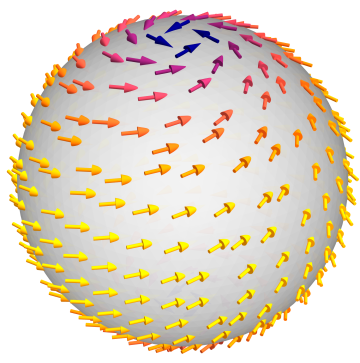
\includegraphics[width=160.28pt,height=161.62pt]{rotation.pdf}};
	
	%Image [id:dp48213474837212833] 
	\draw (474.86,115.75) node  {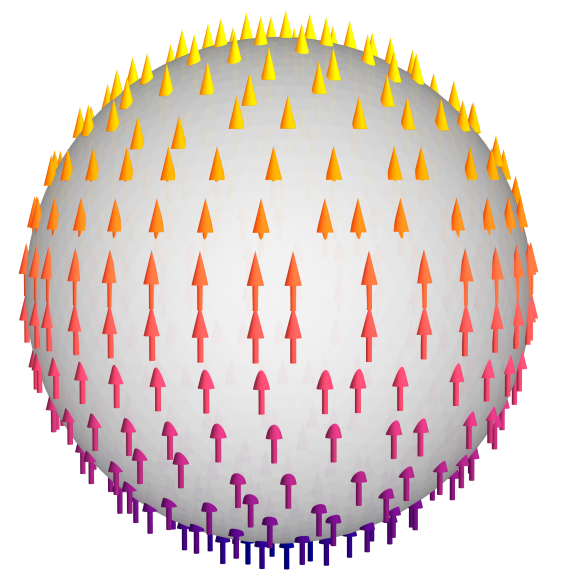
\includegraphics[width=160.28pt,height=161.62pt]{boost.pdf}};
	
	%Image [id:dp180039259569454] 
	\draw (324.5,335.25) node  {\includegraphics[width=170.25pt,height=159.37pt]{four screw.pdf}};
	
	%Straight Lines [id:da15923397993352584] 
	\draw    (289,117.22) -- (360.7,117.22) ;
	%Straight Lines [id:da09146095317161684] 
	\draw    (324.85,117.22) -- (324.85,227.23) ;
	\draw [shift={(324.85,230.23)}, rotate = 270] [fill={rgb, 255:red, 0; green, 0; blue, 0 }  ][line width=0.08]  [draw opacity=0] (10.72,-5.15) -- (0,0) -- (10.72,5.15) -- (7.12,0) -- cycle    ;
	
	% Text Node
	\draw (249,452) node [anchor=north west][inner sep=0.75pt]   [align=left] {effect of a four-screw};
	% Text Node
	\draw (103,233) node [anchor=north west][inner sep=0.75pt]   [align=left] {effect of a rotation};
	% Text Node
	\draw (414,234) node [anchor=north west][inner sep=0.75pt]   [align=left] {effect of a boost};
	
	
\end{tikzpicture}
	\caption{将不同洛伦兹变换在黎曼球上可视化}
	\label{fig:visualization of lorentz transformation}
\end{figure}

如果洛伦兹变换保持不变的两个类光方向重合,那么我们将这种情况称作类光旋转(null rotation)。我们可以将不动点定为$\zeta =\infty $,这时自旋变换就为
\begin{equation*}
	\tilde{\zeta } =\zeta +\beta ,
\end{equation*}
自旋变换矩阵就为
\begin{equation*}
	\begin{pmatrix}
		\tilde{\xi }\\
		\tilde{\eta }
	\end{pmatrix} =\pm \begin{pmatrix}
		1 & \beta \\
		0 & 1
	\end{pmatrix}\begin{pmatrix}
		\xi \\
		\eta 
	\end{pmatrix} .
\end{equation*}
其可视化效果如图\ref{fig:visualization of null rotation}所示。

\begin{figure}[h]
	\centering
	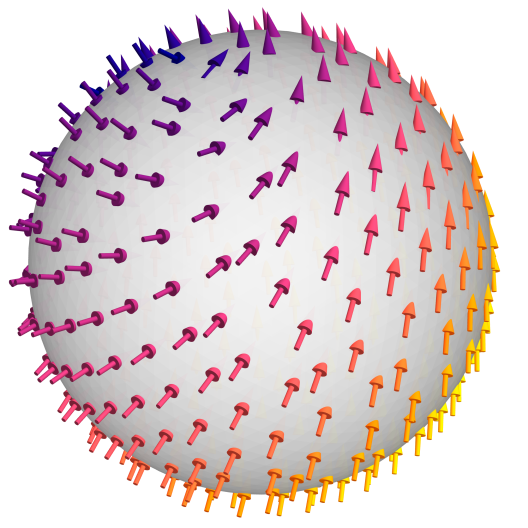
\includegraphics[width=160.28pt,height=161.62pt]{null rotation.pdf}
	\caption{类光旋转可视化化}
	\label{fig:visualization of null rotation}
\end{figure}

\section{类光旗帜与自旋矢量*}

本节的目的是让我们对自旋矢量有一个直观的几何理解。我们知道复数对$( \xi ,\eta )$定义了一个自旋矢量$\boldsymbol{\kappa }$,这与闵氏向量空间中的类光矢量$\boldsymbol{K}$有对应关系\ref{eq:real and complex coordinate}。但我们知道如果用$( \xi ,\eta )$作为$\boldsymbol{K}$的坐标,有冗余自由度$\xi \mapsto \mathrm{e}^{\mathrm{i} \theta } \xi ,\eta \mapsto \mathrm{e}^{\mathrm{i} \theta } \eta $。这个变换很容易让我们想到三维空间中的旋转,因此我们想要将这个冗余自由度阐释为一个“几何结构”,在这个结构之外,多余的自由度可以被缩减到一个符号的不确定性。这个几何结构就是所谓\textbf{类光旗帜}(null flag),即$\boldsymbol{K}$能对应到一个平面相位意义上的$\xi ,\eta $,我们只需要考虑这个“旗帜面”。



除此之外,注意我们所寻找的$( \xi ,\eta )$的几何结构是“内禀”的,即不依赖于坐标的选取。例如考虑自旋变换诱导的被动洛伦兹变换,这样的变换并不会改变$\boldsymbol{\kappa }$的几何结构。



我们的思路是首先在所有类光方向的曲面$\mathcal{S}^{+}$上描述$( \xi ,\eta )$的几何结构,随后再将其引入到$\mathbb{V}$上。


\subsection{$S^{+}$上的描述}

我们知道$\mathcal{S}^{+}$上的点可以与复数$\zeta \equiv \xi /\eta $一一对应,但除了这个比值之外,如果我们知道了表示$\zeta $的点$P$处的实切向量$\mathbf{L}$,那么$\xi ,\eta $也能独立地被表示出来。我们知道$\mathcal{S}^{+}$(的切空间)上的实的切向量可以被表示为
\begin{equation*}
	\mathbf{L} =\lambda \frac{\partial }{\partial \zeta } +\overline{\lambda }\frac{\partial }{\partial \overline{\zeta }} ,
\end{equation*}
其中我们需要选择系数让$\mathbf{L}$是实的。如果$\lambda ( \xi ,\eta )$可以表示为$\xi ,\eta $的定值,这意味着我们需要$\mathbf{L}$在自旋变换下是不变的,即
\begin{equation}
	\lambda '\frac{\partial }{\partial \zeta '} +\overline{\lambda } '\frac{\partial }{\partial \overline{\zeta } '} =\lambda \frac{\partial }{\partial \zeta } +\overline{\lambda }\frac{\partial }{\partial \overline{\zeta }} ,
	\label{eq:invariance of L}
\end{equation}
其中
\begin{equation*}
	\zeta '=\frac{\xi '}{\eta '} =\frac{\alpha \xi +\beta \eta }{\gamma \xi +\delta \eta } =\frac{\alpha \zeta +\beta }{\gamma \zeta +\delta } .
\end{equation*}
那么利用链式法则:
\begin{equation}
	\frac{\partial }{\partial \zeta } =\frac{\partial \zeta '}{\partial \zeta }\frac{\partial }{\partial \zeta '} =\frac{\alpha \delta -\beta \gamma }{(\delta +\gamma \zeta )^{2}}\frac{\partial }{\partial \zeta '} =(\delta +\gamma \zeta )^{-2}\frac{\partial }{\partial \zeta '} =\eta ^{2} \eta ^{\prime -2}\frac{\partial }{\partial \zeta '} .
	\label{eq:chain rule of xi}
\end{equation}
代回\ref{eq:invariance of L}并要求系数相等,我们有
\begin{equation*}
	\lambda '( \xi ',\eta ') \eta ^{\prime 2} =\lambda ( \xi ,\eta ) \eta ^{2} ,
\end{equation*}
这意味着我们必须要求$\lambda $对$\eta $的依赖关系为某个数字乘以$\eta ^{-2}$.我们选取
\begin{equation*}
	\lambda =-\frac{1}{\sqrt{2}} \eta ^{-2} ,
\end{equation*}
那么我们有
\begin{equation}
	\mathbf{L} =-\frac{1}{\sqrt{2}}\left( \eta ^{-2}\frac{\partial }{\partial \zeta } +\overline{\eta }^{-2}\frac{\partial }{\partial \overline{\zeta }}\right) .
	\label{eq:expression of L}
\end{equation}


反过来,如果我们知道$P$点以及$P$点处的$\mathbf{L}$,那么我们就可以将$( \zeta ,\eta )$确定到相差一个符号。因为通过$\mathbf{L}$的具体形式\ref{eq:expression of L},我们可以对比系数给出$\eta ^{2}$,根据$P$我们可以知道$\zeta $,从而反推出$\pm ( \xi ,\eta )$。



等价地,我们可以根据
\begin{equation*}
	\eta ^{2}\mathrm{d} \zeta =\eta \mathrm{d} \xi -\xi \mathrm{d} \eta ,
\end{equation*}
给出
\begin{equation*}
	\eta ^{\prime 2}\mathrm{d} \zeta '=\eta ^{2}\mathrm{d} \zeta ,
\end{equation*}
这与\ref{eq:chain rule of xi}等价。


\subsection{$\mathbb{V}$上的表述}

$\mathcal{S}^{+}$上的切向量$\mathbf{L}$自然诱导出了作为子空间的$S^{+}$上的切向量$\boldsymbol{L}$,而$S^{+}$上的坐标通过\ref{eq:coordinate of stereographic projection}自然与$\mathbb{V}$中的坐标相联系,那么我们可以写出
\begin{equation*}
	\boldsymbol{L} =-\frac{1}{\sqrt{2}}\left( \eta ^{-2}\frac{\partial }{\partial \zeta } +\overline{\eta }^{-2}\frac{\partial }{\partial \overline{\zeta }}\right) =L^{a}\frac{\partial }{\partial x^{a}} ,
\end{equation*}
其中$x^{a}$是$\mathbb{V}$中的坐标。选定参数$x^{0} =1$,通过\ref{eq:coordinate of stereographic projection},我们知道
\begin{equation*}
	\frac{\partial x^{0}}{\partial \zeta } =0,\frac{\partial x^{1}}{\partial \zeta } =\frac{1-\zeta ^{2}}{(\zeta \zeta +1)^{2}} ,\frac{\partial x^{2}}{\partial \zeta } =\frac{1+\zeta ^{2}}{1(\zeta \zeta +1)^{2}} ,\frac{\partial x^{3}}{\partial \zeta } =\frac{2\zeta }{(\zeta \overline{\zeta } +1)^{2}}
\end{equation*}
根据链式法则:
\begin{equation*}
	L^{a}\frac{\partial }{\partial x^{a}} =-\frac{1}{\sqrt{2}}\left( \eta ^{-2}\frac{\partial x^{a}}{\partial \zeta } +\overline{\eta }^{-2}\frac{\partial x^{a}}{\partial \zeta }\right)\frac{\partial }{\partial x^{a}}
\end{equation*}
我们有:
\begin{equation*}
	\begin{aligned}
		L^{0} & =0, & L^{1} & =\frac{\xi ^{2} +\overline{\xi }^{2} -\eta ^{2} -\overline{\eta }^{2}}{\sqrt{2} (\xi \overline{\xi } +\eta \overline{\eta } )^{2}} ,\\
		L^{2} & =\frac{\xi ^{2} -\overline{\xi }^{2} +\eta ^{2} -\overline{\eta }^{2}}{\sqrt{2}\mathrm{i} (\xi \overline{\xi } +\eta \overline{\eta } )^{2}} , & L^{3} & =\frac{-\sqrt{2} (\xi \eta +\overline{\xi }\overline{\eta } )}{(\xi \xi +\eta \overline{\eta } )^{2}} .
	\end{aligned}
\end{equation*}
我们容易发现$\boldsymbol{L}$的范数为
\begin{equation*}
	\| \boldsymbol{L} \| =L^{a} L^{b} \eta _{ab} =\frac{-2}{(\xi \overline{\xi } +\eta \overline{\eta } )^{2}} .
\end{equation*}
注意,这和\ref{eq:homogeneous coordinate of stereoprojection}式的分母一致,也就是我们用来构造$\boldsymbol{K} \equiv \overrightarrow{OR}$的比例因子。这意味着$\boldsymbol{L}$是单位矢量,当且仅当$\boldsymbol{K}$定义了一个在$S^{+}$上的点$P$。如果$( \xi ,\eta )$与$(\tilde{\xi } ,\tilde{\eta })$两点由洛伦兹变换连接,我们很容易发现$L^{a}$之间相差的并不是洛伦兹变换,因为$\boldsymbol{L}$垂直于$S^{+}$意味着与$t$轴正交,但洛伦兹变换显然不保持这个性质。但是,$\boldsymbol{K}$与$\boldsymbol{L}$构成的平面$\hat{\upPi }$却是不变的,即它与坐标无关,因此可以被看做作$\mathbb{V}$中的几何结构。

\begin{figure}[h]
	\centering
	

% Gradient Info

\tikzset {_xfijtitct/.code = {\pgfsetadditionalshadetransform{ \pgftransformshift{\pgfpoint{-69 bp } { 489 bp }  }  \pgftransformscale{3 }  }}}
\pgfdeclareradialshading{_4ys9j1xwk}{\pgfpoint{24bp}{-192bp}}{rgb(0bp)=(0.96,0.96,0.96);
	rgb(0bp)=(0.96,0.96,0.96);
	rgb(5.25bp)=(0.86,0.86,0.89);
	rgb(12.25bp)=(0.72,0.73,0.78);
	rgb(20bp)=(0.87,0.87,0.89);
	rgb(25bp)=(0.96,0.96,0.96);
	rgb(400bp)=(0.96,0.96,0.96)}

% Gradient Info

\tikzset {_34dxukbo6/.code = {\pgfsetadditionalshadetransform{ \pgftransformshift{\pgfpoint{0 bp } { 0 bp }  }  \pgftransformrotate{0 }  \pgftransformscale{2 }  }}}
\pgfdeclarehorizontalshading{_pi2xaa4p6}{150bp}{rgb(0bp)=(0.6,0.85,1);
	rgb(37.5bp)=(0.6,0.85,1);
	rgb(62.5bp)=(0,0.5,0.5);
	rgb(100bp)=(0,0.5,0.5)}

% Gradient Info

\tikzset {_gw9u3nn4y/.code = {\pgfsetadditionalshadetransform{ \pgftransformshift{\pgfpoint{0 bp } { 0 bp }  }  \pgftransformrotate{0 }  \pgftransformscale{2 }  }}}
\pgfdeclarehorizontalshading{_2xbmbn3l0}{150bp}{rgb(0bp)=(0.6,0.85,1);
	rgb(37.5bp)=(0.6,0.85,1);
	rgb(62.5bp)=(0,0.5,0.5);
	rgb(100bp)=(0,0.5,0.5)}

% Gradient Info

\tikzset {_9byeair1q/.code = {\pgfsetadditionalshadetransform{ \pgftransformshift{\pgfpoint{0 bp } { 0 bp }  }  \pgftransformrotate{0 }  \pgftransformscale{2 }  }}}
\pgfdeclarehorizontalshading{_o1fem7bmr}{150bp}{rgb(0bp)=(0.71,0.74,0.78);
	rgb(37.5bp)=(0.71,0.74,0.78);
	rgb(46.5bp)=(0.51,0.55,0.58);
	rgb(62.5bp)=(0.16,0.2,0.23);
	rgb(100bp)=(0.16,0.2,0.23)}

% Gradient Info

\tikzset {_echxgy7iy/.code = {\pgfsetadditionalshadetransform{ \pgftransformshift{\pgfpoint{13.14 bp } { 16.79 bp }  }  \pgftransformscale{1.46 }  }}}
\pgfdeclareradialshading{_31p2pzfdp}{\pgfpoint{-16bp}{-8bp}}{rgb(0bp)=(0.97,0.97,0.97);
	rgb(0bp)=(0.97,0.97,0.97);
	rgb(25bp)=(0.72,0.73,0.78);
	rgb(400bp)=(0.72,0.73,0.78)}
\tikzset{every picture/.style={line width=0.75pt}} %set default line width to 0.75pt        

\begin{tikzpicture}[x=0.75pt,y=0.75pt,yscale=-1,xscale=1]
	%uncomment if require: \path (0,137); %set diagram left start at 0, and has height of 137
	
	%Shape: Triangle [id:dp18085529825630564] 
	\draw  [draw opacity=0][shading=_4ys9j1xwk,_xfijtitct] (203.92,121.29) -- (276.42,37.67) -- (131.41,37.67) -- cycle ;
	%Shape: Parallelogram [id:dp9228773357244249] 
	\draw  [fill={rgb, 255:red, 255; green, 255; blue, 255 }  ,fill opacity=1 ] (117.45,6.93) -- (309.46,6.93) -- (290.38,66.78) -- (98.37,66.78) -- cycle ;
	%Straight Lines [id:da7856751732458289] 
	\draw [shading=_pi2xaa4p6,_34dxukbo6]   (203.92,121.29) -- (156.01,66.83) ;
	%Straight Lines [id:da530742601835525] 
	\draw [shading=_2xbmbn3l0,_gw9u3nn4y]   (203.92,121.29) -- (253.01,65.83) ;
	\draw [shift={(203.92,121.29)}, rotate = 311.51] [color={rgb, 255:red, 0; green, 0; blue, 0 }  ][fill={rgb, 255:red, 0; green, 0; blue, 0 }  ][line width=0.75]      (0, 0) circle [x radius= 3.35, y radius= 3.35]   ;
	%Straight Lines [id:da4568538254779688] 
	\draw  [dash pattern={on 4.5pt off 4.5pt}]  (134.01,41.57) -- (156.01,66.83) ;
	%Straight Lines [id:da7131966021543883] 
	\draw  [dash pattern={on 4.5pt off 4.5pt}]  (274.83,40.85) -- (253.01,65.83) ;
	%Shape: Ellipse [id:dp8890884080819843] 
	\draw  [color={rgb, 255:red, 208; green, 2; blue, 27 }  ,draw opacity=1 ][line width=1.5]  (132,36.85) .. controls (132,26.22) and (164.2,17.6) .. (203.92,17.6) .. controls (243.64,17.6) and (275.83,26.22) .. (275.83,36.85) .. controls (275.83,47.49) and (243.64,56.1) .. (203.92,56.1) .. controls (164.2,56.1) and (132,47.49) .. (132,36.85) -- cycle ;
	%Straight Lines [id:da09373596447493804] 
	\draw    (223.01,55.31) -- (203.92,121.29) ;
	\draw [shift={(214.6,84.36)}, rotate = 106.14] [fill={rgb, 255:red, 0; green, 0; blue, 0 }  ][line width=0.08]  [draw opacity=0] (7.14,-3.43) -- (0,0) -- (7.14,3.43) -- (4.74,0) -- cycle    ;
	%Shape: Polygon [id:ds8121831694427222] 
	\path  [shading=_o1fem7bmr,_9byeair1q] (257.01,18.31) -- (231.01,29.31) -- (235.01,14.31) -- cycle ; % for fading 
	\draw   (257.01,18.31) -- (231.01,29.31) -- (235.01,14.31) -- cycle ; % for border 
	
	%Straight Lines [id:da8477468495579272] 
	\draw    (223.01,55.31) -- (234.44,16.23) ;
	\draw [shift={(235.01,14.31)}, rotate = 106.31] [color={rgb, 255:red, 0; green, 0; blue, 0 }  ][line width=0.75]    (7.65,-2.3) .. controls (4.86,-0.97) and (2.31,-0.21) .. (0,0) .. controls (2.31,0.21) and (4.86,0.98) .. (7.65,2.3)   ;
	\draw [shift={(223.01,55.31)}, rotate = 286.31] [color={rgb, 255:red, 0; green, 0; blue, 0 }  ][fill={rgb, 255:red, 0; green, 0; blue, 0 }  ][line width=0.75]      (0, 0) circle [x radius= 2.34, y radius= 2.34]   ;
	%Straight Lines [id:da15925016913815626] 
	\draw [color={rgb, 255:red, 74; green, 144; blue, 226 }  ,draw opacity=1 ]   (278.02,50.57) -- (223.01,55.31) ;
	\draw [shift={(281.01,50.31)}, rotate = 175.07] [fill={rgb, 255:red, 74; green, 144; blue, 226 }  ,fill opacity=1 ][line width=0.08]  [draw opacity=0] (7.14,-3.43) -- (0,0) -- (7.14,3.43) -- (4.74,0) -- cycle    ;
	%Curve Lines [id:da02129065464097457] 
	\draw    (320.38,69.78) .. controls (359.98,40.08) and (379.98,98.59) .. (419.19,70.65) ;
	\draw [shift={(420.38,69.78)}, rotate = 143.13] [color={rgb, 255:red, 0; green, 0; blue, 0 }  ][line width=0.75]    (10.93,-3.29) .. controls (6.95,-1.4) and (3.31,-0.3) .. (0,0) .. controls (3.31,0.3) and (6.95,1.4) .. (10.93,3.29)   ;
	%Shape: Circle [id:dp7494161810872726] 
	\path  [shading=_31p2pzfdp,_echxgy7iy] (442,70.43) .. controls (442,46.96) and (461.03,27.93) .. (484.5,27.93) .. controls (507.98,27.93) and (527.01,46.96) .. (527.01,70.43) .. controls (527.01,93.9) and (507.98,112.93) .. (484.5,112.93) .. controls (461.03,112.93) and (442,93.9) .. (442,70.43) -- cycle ; % for fading 
	\draw  [color={rgb, 255:red, 208; green, 2; blue, 27 }  ,draw opacity=1 ] (442,70.43) .. controls (442,46.96) and (461.03,27.93) .. (484.5,27.93) .. controls (507.98,27.93) and (527.01,46.96) .. (527.01,70.43) .. controls (527.01,93.9) and (507.98,112.93) .. (484.5,112.93) .. controls (461.03,112.93) and (442,93.9) .. (442,70.43) -- cycle ; % for border 
	
	%Straight Lines [id:da855599687264156] 
	\draw [color={rgb, 255:red, 74; green, 144; blue, 226 }  ,draw opacity=1 ]   (546.02,81.57) -- (491.01,86.31) ;
	\draw [shift={(549.01,81.31)}, rotate = 175.07] [fill={rgb, 255:red, 74; green, 144; blue, 226 }  ,fill opacity=1 ][line width=0.08]  [draw opacity=0] (7.14,-3.43) -- (0,0) -- (7.14,3.43) -- (4.74,0) -- cycle    ;
	%Straight Lines [id:da2554725584191] 
	\draw    (491.01,86.31) ;
	\draw [shift={(491.01,86.31)}, rotate = 0] [color={rgb, 255:red, 0; green, 0; blue, 0 }  ][fill={rgb, 255:red, 0; green, 0; blue, 0 }  ][line width=0.75]      (0, 0) circle [x radius= 2.34, y radius= 2.34]   ;
	%Straight Lines [id:da514198553655629] 
	\draw [color={rgb, 255:red, 74; green, 144; blue, 226 }  ,draw opacity=1 ] [dash pattern={on 4.5pt off 4.5pt}]  (433.01,91.31) -- (491.01,86.31) ;
	
	
	% Text Node
	\draw (211,113.5) node [anchor=north west][inner sep=0.75pt]    {$O$};
	% Text Node
	\draw (154,94.5) node [anchor=north west][inner sep=0.75pt]  [font=\small]  {$\mathcal{S}^{+}$};
	% Text Node
	\draw (111,40) node [anchor=north west][inner sep=0.75pt]  [color={rgb, 255:red, 208; green, 2; blue, 27 }  ,opacity=1 ]  {$S^{+}$};
	% Text Node
	\draw (205.92,39.85) node [anchor=north west][inner sep=0.75pt]    {$P$};
	% Text Node
	\draw (191,80) node [anchor=north west][inner sep=0.75pt]    {$\boldsymbol{K}$};
	% Text Node
	\draw (281,38) node [anchor=north west][inner sep=0.75pt]  [color={rgb, 255:red, 74; green, 144; blue, 226 }  ,opacity=1 ]  {$\boldsymbol{L}$};
	% Text Node
	\draw (215,7.94) node [anchor=north west][inner sep=0.75pt]    {$R$};
	% Text Node
	\draw (551,70) node [anchor=north west][inner sep=0.75pt]  [color={rgb, 255:red, 74; green, 144; blue, 226 }  ,opacity=1 ]  {$\boldsymbol{L}$};
	% Text Node
	\draw (475.92,68.85) node [anchor=north west][inner sep=0.75pt]    {$P$};
	% Text Node
	\draw (457,9) node [anchor=north west][inner sep=0.75pt]  [color={rgb, 255:red, 208; green, 2; blue, 27 }  ,opacity=1 ]  {$S^{+}$};
	
	
\end{tikzpicture}
	\caption{类光旗帜。注意这里$\boldsymbol{L}$并不是只有一个方向。}
	\label{fig:null flag}
\end{figure}

这里,$\hat{\upPi }$中的向量为
\begin{equation*}
	a\boldsymbol{K} +b\boldsymbol{L} ,
\end{equation*}
而我们选择$b >0$并称这个半平面为$\upPi $。我们可以看到,$\upPi $可以将$( \xi ,\eta )$决定到只差一个符号:$\boldsymbol{K}$将$\eta ,\xi $决定到相差一个全局相位,而$\boldsymbol{L}$的方向告诉我们$\eta $的相位。我们称$\upPi $与$\boldsymbol{K}$为类光旗帜(null flag)而称$\boldsymbol{K}$为旗杆(flagpole),$ $$\upPi $为旗帜面(flag plane)。



现在考虑一般的自旋变换对光旗的影响。考虑变换
\begin{equation*}
	( \xi ,\eta ) \mapsto ( \lambda \xi ,\lambda \eta ) ,\lambda \in \mathbb{C} \setminus \{0\} .
\end{equation*}
令$\lambda =r\mathrm{e}^{\mathrm{i} \theta }$,我们发现$\theta =0$时,旗帜面不变,旗杆变长$r^{2}$倍;当$r=1$时,旗杆不变,旗帜面旋转$2\theta $,因为$\boldsymbol{L}$与$\eta $呈二次相关性。



现在,如果我们考虑一个连续的旋转$( \xi ,\eta ) \mapsto (\mathrm{e}^{\mathrm{i} \theta } \xi ,\mathrm{e}^{\mathrm{i} \theta } \eta )$,其中$\theta $从$0$旋转到$\pi $,我们给出
\begin{equation*}
	( \xi ,\eta ) \mapsto ( -\xi ,-\eta ) ,
\end{equation*}
但是我们的旗帜面旋转了$2\pi $。将$\theta $继续旋转到$2\pi $,我们会给出原来的点$( \xi ,\eta )$,但旗帜面旋转了$4\pi $,这意味着如果我们想要在$\mathbb{V}$中建立一个消除符号不确定性的局域几何结构是不可能的。因为我们想要在类光旗帜中间添加的$\mathbb{V}$中的每一个局域的几何结构在旋转了$2\pi $后都会回到原来的状态,但是$( \xi ,\eta )$却会多一个全局的负号。为了更清楚地看到这一点,不妨选择$( \xi ,\eta ) =( 0,1) \mapsto (0,\mathrm{e}^{\mathrm{i} \theta } )$。当$\theta $旋转到$\pi $时,自旋变换为$-\boldsymbol{I}$,但是洛伦兹变换却是单位元,这意味着任何$V$中的几何结构都会被这个洛伦兹变换转回到它原来的状态,即使$( \xi ,\eta )$已经变成了$( -\xi ,-\eta )$。



这意味着我们应当扩充常规意义下的$\mathbb{V}$中的“几何”对象,这样的对象在旋转$2\pi $后并不回到原来的状态,当旋转$4\pi $时才回到原来的状态,这就是\textbf{旋量对象}(spinorial objects)。


\section{旋量对象与自旋结构}

众所周知,三维空间的旋转由$SO( 3)$描述,而其基本群$\pi _{1}( SO( 3)) =\mathbb{Z}_{2}$,这意味着即使\textbf{只}考虑$SO( 3)$群,我们也可以获得两种不同的“回到原点”的旋转,即旋转$2\pi $和旋转$4\pi $是$SO( 3)$的基本群中的两个元素。在$SO( 3)$的拓扑空间$\mathbb{R} P^{3}$中,旋转$2\pi $的曲线(圈)不可以被连续地变换到一个点,而旋转$4\pi $的曲线则可以。例如考虑狄拉克的皮带实验,这说明考虑旋转时不应仅仅考虑初末状态,还应该考虑\textbf{路径}。当然对于绝大多数拓扑平凡的物体以及其旋转来说,$2\pi $的旋转与$4\pi $的旋转没有区别。



现在我们来考虑一个拓扑空间$T$的万有覆盖空间(universal covering space)$\tilde{T}$。考虑$T$中的原点$O$与任意一点$X$,从$O$到$X$有不同的路径的种类(class),每一类路径中的任意一条路径都可以连续变成其他路径,而不同类路径之间的路径之间没有连续变换。而$\tilde{T}$中的元素实际上是$T$中从$O$到$X$的\textbf{路径},其中$X$要取遍$T$整个空间。例如,我们考虑$S^{1}$,其上任意一点用$\theta $参数化。那么到这一点的路径的等价类可以由“绕圆转了几圈”来刻画,也即$\mathbb{Z}$。当我们取遍$\theta \in ( 0,2\pi ]$时,所有的路径也就构成了整个实轴,整个过程就是把$S^{1}$展开(unwrap)的过程。因此,$T$的万有覆盖空间实际上就是把$T$从内到外展开后得到的拓扑空间。



那么考虑$SO( 3)$,我们知道其中每一点的路径只有两类,那么其万有覆盖空间就是把$SO( 3)$双重展开(twofold unwrap)后的结果,也就是我们熟悉的$SU( 2)$。同样的,正时正规洛伦兹群$O_{+}^{\uparrow }( 1,3)$的二重覆盖群为$SL( 2,\mathbb{C})$。实际上,$O_{+}^{\uparrow }( 1,3)$的拓扑性质并不比$SO( 3)$复杂,因为每一个洛伦兹变换都可以由旋转与推动复合成,但是推动的“拓扑”是平凡的,只是拉伸,因此$O_{+}^{\uparrow }( 1,3)$的拓扑性质和$SO( 3)$的相同。现在,如果三维空间中,一个物体旋转$2\pi $没有回到原来的状态,而旋转$4\pi $才回到原来的状态,那么我们称这样的物体为旋量对象(spinorial objects)。



现在我们可以给出自旋矢量的几何定义了。考虑$\mathbb{V}$中的光旗$Q$,全部光旗构成的空间为$\mathcal{C}$。下面我们会证明$\mathcal{C} \cong SO( 3) \times \mathbb{R}$,即$\pi _{1}(\mathcal{C}) =\mathbb{Z}_{2}$。我们知道$Q$可以由$P$点及$P$处切矢$\boldsymbol{L}$构造,如果我们在$P$处建立一个$3$维坐标系,$z$轴为$OP$,$x$轴朝着$\boldsymbol{L}$方向,用右手定则补齐$y$轴,我们发现这样一个坐标系对应了$SO( 3)$中的一个点。另一个参数为$\| \boldsymbol{L} \| $的长度,这在拓扑上是平凡的,等价于$\mathbb{R}$,这意味着$\mathcal{C} \cong SO( 3) \times \mathbb{R}$。那么我们称$\tilde{\mathcal{C}}$为旋量化的光旗,其中的元素可以与$\mathbb{V}$中的非零自旋矢量一一对应。每一个$\mathcal{C}$中的$Q$对应了两个自旋矢量$\pm \boldsymbol{\kappa }$。



下面我们来考虑上面的内容如何影响了一个弯曲时空$\mathcal{M}$的\textbf{整体}拓扑结构。目前为止我们考虑的都是时空的局部特征,即我们讨论的光旗都是时空中一点上的。有些时空的背景流形的拓扑结构不平凡,意味着这对局域的拓扑结构有限制。一个很自然的问题是,如果一个时空全空间都能定义像自旋矢量这样的对象,会给出时空的整体拓扑什么约束?



我们考虑这样一个空间$\mathcal{F}$,其中每一个点都代表了$\mathcal{M}$中的一个光旗,我们称这个空间为$\mathcal{M}$的光旗丛(null-flag bundle)。$\mathcal{F}$是一个八维空间,因为$\mathcal{M}$是四维空间,并且任意一点$P$的光旗空间$\mathcal{F}_{P}$也是四维的。现在我们不加证明地给出这样的结论:

\begin{cond}[label={cond:condition of null flag bundle 1}]{流形存在光旗丛的条件}
	如果$\mathcal{M}$上存在光旗丛$\mathcal{F}$,那么$\mathcal{M}$必须是在时间上可定向的。
\end{cond}

这是因为光旗只能在两个光锥中的一个上,我们将那一个光锥定义为指向未来的。

除此之外,由于乘以$\mathrm{e}^{\mathrm{i} \theta }$会将光旗在某个意义下旋转,这意味着我们需要整个时空的定向,因此我们还需要条件:

\begin{cond}[label={cond:condition of null flag bundle 2}]{流形存在光旗丛的条件}
	如果$\mathcal{M}$上存在光旗丛$\mathcal{F}$,那么$\mathcal{M}$必须是在整个时空上是可定向的。
\end{cond}

注意,条件\ref{cond:condition of null flag bundle 1}和条件\ref{cond:condition of null flag bundle 2}是两个不同的条件。但仅仅是这两个条件还不够,$\mathcal{M}$上还应该需要能定义所谓的\textbf{自旋结构}(spin structure)。注意,这里的旋量结构和$\mathcal{M}$上是否能存在特定的旋量场是不一样的,后者更像是考虑例如$S^{2}$上是否能存在处处非零向量场这样的问题。粗略地说,存在自旋结构要求我们不仅在流形上某一点确定自旋矢量的方向,还需要能在流形的每一点确定。而且,即使存在,不同流形上的自旋结构可能不是唯一的。构造流形上的自旋结构有各种困难,但是人们还是证明了,$\mathcal{M}$上存在自旋结构的充要条件为拓扑不变量第二Stieffel-Whitney类$w_{2} =0$。这粗略等价于

\begin{cond}[label={cond:condition of spin structure}]{流形存在自旋结构的条件}
	对于流形$\mathcal{M}$(维数大于2)上任意闭的$2-$曲面$\mathcal{S}$,都存在一个$\mathcal{M}$的$n-1$个连续切向量场,且这些切向量在$\mathcal{S}$上每一点都是线性无关的。如果$\mathcal{M}$可定向(即$w_{1} =0$),那么$n-1$应该换成$n$。
\end{cond}

如果条件\ref{cond:condition of null flag bundle 1},\ref{cond:condition of null flag bundle 2},\ref{cond:condition of spin structure}都被满足,那么我们称这个流形上有所谓的\textbf{旋量结构}(spinor structure)。即,如果$\mathcal{M}$有旋量结构,那么我们之前所描述的基于光旗和自旋矢量的旋量系统都是存在的,也即$\mathcal{F}$的双重覆盖空间$\mathcal{F} '$是存在的。如果$\mathcal{M}$是单连通的,那么$\mathcal{F} '=\tilde{\mathcal{F}}$,但如果$\mathcal{M}$不是单连通的,旋量结构并不唯一,即$\mathcal{F} '\neq \tilde{\mathcal{F}}$。如果$\mathcal{M}$中有$k$个独立的圈(loop),那么实际上$\mathcal{M}$上有$2^{k}$种不同的旋量结构。

除此之外,如果$\mathcal{M}$上没有闭合类时线,$\mathcal{M}$应当是非紧的流形,这种情况下我们有这样的定理:

\begin{them}[label={them:condition of spin structure of non-compact spacetime}]{非紧空间存在旋量结构的条件}
	如果$\mathcal{M}$是一个非紧的时空,那么这个时空存在旋量结构的充要条件是,在$\mathcal{M}$每一点的切空间上存在连续的闵氏标架场。
\end{them}

如果一个时空是非单连通的,虽然上面有多重旋量结构,但是随着定理 \ref{them:condition of spin structure of non-compact spacetime} 给出的标架场的选定,对应的旋量结构也被确定了。但即使$\mathcal{M}$是单连通的,闵氏标架场的选择仍然是不唯一的。



我们需要指出,定理\ref{them:condition of spin structure of non-compact spacetime}中非紧的前提条件是非常有物理背景的,同时我们也有很多理由相信时空应当存在旋量结构。因为统计力学倾向于告诉我们时间是定向流动的,宇称($P$对称性破缺)不守恒天然给我们了一个“空间方向”的定义,因此空间上的定向也很可能是存在的,同时,例如费米子场这样的旋量场在时空中的存在性意味着时空中很可能存在自旋结构,因此我们很倾向于相信存在一个在整个上时空定义的正时正规闵氏标架场。

\chapter{$\mathfrak{S}$-模上的咏叹调——抽象指标以及旋量代数}

为什么我们需要抽象指标记号?首先注意到一个事实:如果对两个不同的复向量空间做张量积,那么它们张量积的顺序是无所谓的,因为我们发现有一个自然同构$\sum _{i} v_{i} \otimes w_{i} \mapsto \sum _{i} w_{i} \otimes v_{i}$。但是当两个空间相同的时候,张量积的\textbf{顺序}就变得重要了,因为一般来说$v_{1} \otimes v_{2} -v_{2} \otimes v_{1} \neq 0$。因此,一个自然的想法是,我们不再处理张量积空间$V\otimes V\otimes V$,而是处理张量积空间$V^{a} \otimes V^{b} \otimes V^{c}$,这意味着我们可以\textbf{暂时}将不同标记的空间视为不同的空间。举个例子,考虑$v_{1}^{a} \otimes v_{2}^{b} \otimes v_{3}^{c}$,如果忽略自然同构关系,对$1,3$做置换,得到$v_{3}^{c} \otimes v_{2}^{b} \otimes v_{1}^{a}$。这时候,我们再借助$a,c$之间的同构,我们有
\begin{equation*}
	v_{3}^{c} \otimes v_{2}^{b} \otimes v_{1}^{a} \mapsto v_{3}^{a} \otimes v_{2}^{b} \otimes v_{1}^{c} ,
\end{equation*}
这意味着通过置换$a,c$我们构建了一个$V^{a} \otimes V^{b} \otimes V^{c}$到自身的非恒等映射:
\begin{equation*}
	v_{1}^{a} \otimes v_{2}^{b} \otimes v_{3}^{c} \mapsto v_{3}^{a} \otimes v_{2}^{b} \otimes v_{1}^{c} .
\end{equation*}
这些用来“强行区分”相同空间以便用于跟踪的记号称为\textbf{抽象指标}。张量积的交换通过抽象指标的\textbf{置换}来表达。我们将上式简写为$v_{1}^{a} v_{2}^{b} v_{3}^{c} \mapsto v_{1}^{c} v_{2}^{b} v_{3}^{a}$,或者$T^{abc} \mapsto T^{cba}$。

虽然抽象指标记号带有指标,但是它并不依赖于任何基的选择。除此之外,其运算法则与具体指标是一致的,区别只是概念上的阐释,但是当我们引入微分以后,两者的差别就会凸显出来了,同时这也导向了旋量代数的出现。


\section{抽象指标*}
\subsection{用抽象指标定义张量}

如果使用具体指标,指标之间的置换是非常自然的,例如
\begin{equation*}
	H_{\rho }^{\alpha \beta \gamma } =A_{\rho }^{\beta \alpha \gamma } ,
\end{equation*}
之所以要考虑指标之间的置换是因为这条运算与张量的分量的变换规则是对易的:
\begin{equation*}
	A_{\rho \cdots \tau }^{\alpha \cdots \gamma } \mapsto A_{\varphi \cdots \psi }^{\lambda \cdots \nu } t_{\lambda }^{\alpha } \cdots t_{\nu }^{\gamma } T_{\rho }^{\varphi } \cdots T_{\tau }^{\psi } ,
\end{equation*}
这里
\begin{equation*}
	t_{\beta }^{\alpha } T_{\gamma }^{\beta } =\delta _{\gamma }^{\alpha } .
\end{equation*}
但是具体指标一个很重要的问题就是它依赖于坐标系的选取,这会在我们想要推导一些广泛结论时出现问题,于是一个很自然的想法是使用抽象的张量代数,即只用张量的运算法则定义张量。但是,这样做的问题在于如果我们将指标去掉,只考虑$\boldsymbol{AB}$或$\boldsymbol{BA}$这样的抽象张量对象,我们无法表现张量指标之间的对称性。于是,我们很自然的想引入一种抽象指标记号,这里的指标并不代表一些数字,也不依赖于坐标系,只是用来标记张量的类型以及指标之间的对称关系。例如符号$V^{\boldsymbol{a}}$并不代表$n$元组$(V^{1} ,V^{2} ,\cdots V^{n} )$,而只是一个抽象的向量空间或模\footnote{这里我们使用“模”这个术语是因为,如果考虑一个数域上的向量空间,那么这个数域自然是可除的,但如果考虑整个空间上的向量场,这个向量场定义在一个“标量场”(或者交换环)上,那么这个标量场有可能不是可逆的。例如$h,k$是两个不同的标量场,有可能$h$仅仅在$k$消失的区域上非零,这意味着$hk=0$但是这两个标量场都不为零。因此,我们称这样的可能不是可除的交换环为模(module)以区分普通的数域。}中的一个元素。这里,我们用粗体$\boldsymbol{a}$指标表示抽象指标,而正常斜体代表已经选择了坐标系的具体指标。



使用了具体指标就会产生一些非常尴尬的情况,例如对于具体指标,$V^{a} U^{b} -V^{b} U^{a}$在一般情况下非零,但是对于抽象指标,$V^{\boldsymbol{a}} =V^{\boldsymbol{b}} ,U^{\boldsymbol{a}} =U^{\boldsymbol{b}}$,这意味着$V^{\boldsymbol{a}} U^{\boldsymbol{b}} -V^{\boldsymbol{b}} U^{\boldsymbol{a}} =0$。这意味着对于每一个矢量$\boldsymbol{V}$,我们都应该考虑它的无穷多个副本$V^{\boldsymbol{a}} ,V^{\boldsymbol{b}} ,\cdots ,V^{\boldsymbol{a}_{0}} ,\cdots V^{\boldsymbol{a}_{1}} ,\cdots $,其中任何两个都是相同的,但是在表达式中可以被当成不同矢量。同时,$\boldsymbol{V}$所在的整个模$\mathfrak{S}^{\bullet }$也应有无穷多个副本$\mathfrak{S}^{\boldsymbol{a}} ,\mathfrak{S}^{\boldsymbol{b}} ,\cdots ,\mathfrak{S}^{a_{0}} ,\cdots $。这意味着$a\boldsymbol{V} +b\boldsymbol{U} =\boldsymbol{W}$当且仅当$aV^{\boldsymbol{a}} +bU^{\boldsymbol{a}} =W^{\boldsymbol{a}}$,其中$a,b\in \mathfrak{S}$,即标量$a,b,\cdots $构成的交换环。如果定义一个指标集
\begin{equation*}
	\mathcal{L} =\{\boldsymbol{a} ,\boldsymbol{b} ,\cdots ,\boldsymbol{a}_{0} ,\boldsymbol{b}_{0} ,\cdots \} ,
\end{equation*}
那么实际上抽象指标描绘的向量实际上是一个数对$(\boldsymbol{V} ,\boldsymbol{a}) \in \mathfrak{S}^{\bullet } \times \mathcal{L}$,其中$\boldsymbol{V} \in \mathfrak{S}^{\bullet }$,$\boldsymbol{a} \in \mathcal{L}$。

考虑到读者可能对模不熟悉,我们在这里给出其公理化定义。

\begin{defi}[label={defi:fraS and commutative ring}]{$\mathfrak{S}$是有单位元的交换环}
	对于$\mathfrak{S}$中的每一个元素,我们有
	\begin{enumerate}[label=(\alph*)]
		\item $a+b=b+a$
		\item $a+(b+c)=(a+b)+c$
		\item $ab=ba$
		\item $a(bc)=(ab)c$
		\item $a(b+c)=ab+ac$
		\item $\exists 0\in \mathfrak{S}$,s.t. $\forall a\in \mathfrak{S} ,0+a=a$
		\item $\exists 1\in \mathfrak{S}$,s.t. $\forall a\in \mathfrak{S} ,1a=a$
		\item $\forall a\in \mathfrak{S} ,\exists -a\in \mathfrak{S}$,s.t. $a+( -a) =0$。
	\end{enumerate}
\end{defi}

注意,在上述定义中,乘法逆元可能不存在。现在,如果我们有一个无限的指标集$\mathcal{L}$,我们就可以定义所谓的$\mathfrak{S}$-模:

\begin{defi}[label={defi:fraSa}]{$\mathfrak{S}$-模$\mathfrak{S}^{\boldsymbol{a}}$}
	$\mathfrak{S}^{\boldsymbol{a}}$上的加法和数乘运算定义是映射$\mathfrak{S} \times \mathfrak{S}^{\boldsymbol{a}}\rightarrow \mathfrak{S}^{\boldsymbol{a}}$,满足:
	\begin{enumerate}[label=(\alph*)]
		\item $U^{\boldsymbol{a}} +V^{\boldsymbol{a}} =V^{\boldsymbol{a}} +U^{\boldsymbol{a}}$
		\item $U^{\boldsymbol{a}} +(V^{\boldsymbol{a}} +W^{\boldsymbol{a}} )=(U^{\boldsymbol{a}} +V^{\boldsymbol{a}} )+W^{\boldsymbol{a}}$
		\item $a(U^{\boldsymbol{a}} +V^{\boldsymbol{a}} )=aU^{\boldsymbol{a}} +aV^{\boldsymbol{a}}$
		\item $(a+b)U^{\boldsymbol{a}} =aU^{\boldsymbol{a}} +bU^{\boldsymbol{a}}$
		\item $(ab)U^{\boldsymbol{a}} =a(bU^{\boldsymbol{a}} )$
		\item $1U^{\boldsymbol{a}} =U^{\boldsymbol{a}}$
		\item $0U^{\boldsymbol{a}} =0V^{\boldsymbol{a}}$。
	\end{enumerate}
\end{defi}

这里$\mathfrak{S}$中的元素为$( 0,0)$型张量(标量),而$\mathfrak{S}^{\boldsymbol{a}}$中的元素为$( 1,0)$型张量。我们也可以定义其对偶,$( 0,1)$型张量$\mathfrak{S}_{\boldsymbol{a}} ,\mathfrak{S}_{\boldsymbol{b}} ,\cdots $:

\begin{defi}[label={defi:dualfraSa}]{$\mathfrak{S}_{\boldsymbol{a}}$}
	$\mathfrak{S}_{\boldsymbol{a}}$为从$\mathfrak{S}^{\boldsymbol{a}}$到$\mathfrak{S}$的$\mathfrak{S}$-线性映射,即对于每一个元素$Q_{\boldsymbol{a}} \in \mathfrak{S}_{\boldsymbol{a}}$是一个映射$Q_{\boldsymbol{a}} :\mathfrak{S}^{\boldsymbol{a}}\rightarrow \mathfrak{S}$,使得
	\begin{equation*}
		\begin{aligned}
			Q_{\boldsymbol{a}} (U^{\boldsymbol{a}} +V^{\boldsymbol{a}} ) & =Q_{\boldsymbol{a}} (U^{\boldsymbol{a}} )+Q_{\boldsymbol{a}} (V^{\boldsymbol{a}} ),\\
			Q_{\boldsymbol{a}} (aV^{\boldsymbol{a}} ) & =aQ_{\boldsymbol{a}} (V^{\boldsymbol{a}} ).
		\end{aligned}
	\end{equation*}
\end{defi}

一个自然的感觉是$\mathfrak{S}^{\boldsymbol{a}}$与$\mathfrak{S}_{\boldsymbol{a}}$是同构的,但对于一般的交换幺环$\mathfrak{S}$上的模$\mathfrak{S}^{\boldsymbol{a}}$来说,这是\textbf{错误}的。我们称两者同构的模为\textbf{自反}(reflexive)的,我们只考虑这种情况(稍后我们会考虑更加简单的,完全自反的情况)。



下面我们尝试定义张量。我们用两种定义证明张量,而两种定义等价的条件是$\mathfrak{S}^{\boldsymbol{a}}$是完全自反的。



第一类张量(type I tensor)由映射定义。

\begin{defi}[label={defi:tensor of first type}]{第一类张量}
	考虑两个不相交的指标集,$\{\boldsymbol{a} ,\boldsymbol{b} ,\cdots \boldsymbol{d}\}$和$\{\boldsymbol{l} ,\cdots \boldsymbol{n}\}$的势分别为$p,q$,那么一个$( p,q)$型张量是一个$\mathfrak{S}$-多线性映射:
	\begin{equation*}
		A_{\boldsymbol{l} \cdots \boldsymbol{n}}^{\boldsymbol{ab} \cdots \boldsymbol{d}} :\mathfrak{S}_{\boldsymbol{a}} \times \mathfrak{S}_{\boldsymbol{b}} \times \cdots \times \mathfrak{S}_{\boldsymbol{d}} \times \mathfrak{S}^{\boldsymbol{l}} \times \cdots \mathfrak{S}^{\boldsymbol{n}}\rightarrow \mathfrak{S} ,
	\end{equation*}
	其中
	\begin{equation*}
		A_{\boldsymbol{l} \cdots \boldsymbol{n}}^{\boldsymbol{ab} \cdots \boldsymbol{d}} :(Q_{\boldsymbol{a}} ,R_{\boldsymbol{b}} ,\cdots T_{\boldsymbol{d}} ,U^{\boldsymbol{l}} ,\cdots ,W^{\boldsymbol{n}} )\in \mathfrak{S} ,
	\end{equation*}
	其中对这个映射对每个变量都是$\mathfrak{S}$-线性的:
	\begin{equation*}
		A_{\boldsymbol{l} \cdots \boldsymbol{n}}^{\boldsymbol{ab} \cdots \boldsymbol{d}} (aQ_{\boldsymbol{a}} ,\cdots )=aA_{\boldsymbol{l} \cdots \boldsymbol{n}}^{\boldsymbol{ab} \cdots \boldsymbol{d}} (aQ_{\boldsymbol{a}} ,\cdots ),\cdots A_{\boldsymbol{l} \cdots \boldsymbol{n}}^{\boldsymbol{ab} \cdots \boldsymbol{d}} (\cdots ,aW^{\boldsymbol{n}} )=aA_{\boldsymbol{l} \cdots \boldsymbol{n}}^{\boldsymbol{ab} \cdots \boldsymbol{d}} (\cdots ,W^{\boldsymbol{n}} )
	\end{equation*}
	同时对同一个空间$\mathfrak{S}_{\boldsymbol{a}}$中的不同元素$Q_{1\boldsymbol{a}} ,Q_{2\boldsymbol{a}} ,\cdots $也都是线性的:
	\begin{equation*}
		A_{\boldsymbol{l} \cdots \boldsymbol{n}}^{\boldsymbol{ab} \cdots \boldsymbol{d}} (Q_{1\boldsymbol{a}} +Q_{2\boldsymbol{a}} ,\cdots )=A_{\boldsymbol{l} \cdots \boldsymbol{n}}^{\boldsymbol{ab} \cdots \boldsymbol{d}} (Q_{1\boldsymbol{a}} ,\cdots )+A_{\boldsymbol{l} \cdots \boldsymbol{n}}^{\boldsymbol{ab} \cdots \boldsymbol{d}} (Q_{2\boldsymbol{a}} ,\cdots ).
	\end{equation*}
	记这样的张量$A_{\boldsymbol{l} \cdots \boldsymbol{n}}^{\boldsymbol{ab} \cdots \boldsymbol{d}}$所在的空间为$\mathfrak{S}_{\boldsymbol{l} \cdots \boldsymbol{n}}^{\boldsymbol{ab} \cdots \boldsymbol{d}}$。
\end{defi}

我们发现这样的定义根据我们假设的自反性,与原来的$\mathfrak{S}^{\boldsymbol{a}}$的定义是一致的。

现在我们给出不依赖坐标的第二种定义张量的办法:

\begin{defi}[label={defi:tensor of second type}]{第二类张量}
	考虑两个不相交的非零集合$\{\boldsymbol{a} ,\boldsymbol{b} ,\cdots ,\boldsymbol{d}\}$以及$\{\boldsymbol{l} ,\cdots ,\boldsymbol{n}\}$,考虑形式乘积:
	\begin{equation}
		B_{\boldsymbol{l} \cdots \boldsymbol{n}}^{\boldsymbol{ab} \cdots \boldsymbol{d}} =\sum _{i=1}^{m} G_{i}^{\boldsymbol{a}} H_{i}^{\boldsymbol{b}} \cdots J_{i}^{\boldsymbol{d}} L_{i\boldsymbol{l}} \cdots N_{i\boldsymbol{n}} ,
		\label{eq:tensor of second type}
	\end{equation}
	其中形式乘积满足
	\begin{equation*}
		(X^{\boldsymbol{x}} +Y^{\boldsymbol{x}} )C^{\boldsymbol{r}} \cdots E^{\boldsymbol{t}} =X^{\boldsymbol{x}} C^{\boldsymbol{r}} \cdots E^{\boldsymbol{t}} +Y^{\boldsymbol{x}} C^{\boldsymbol{r}} \cdots E^{\boldsymbol{t}} ,
	\end{equation*}
	以及
	\begin{equation*}
		(qX^{\boldsymbol{x}} )Y^{\boldsymbol{e}} C^{\boldsymbol{r}} \cdots E^{\boldsymbol{t}} =X^{\boldsymbol{x}} (qY^{\boldsymbol{e}} )C^{\boldsymbol{r}} \cdots E^{\boldsymbol{t}} .
	\end{equation*}
\end{defi}

我们可以看到,任何第二类张量都自然给出了一个第一类张量:
\begin{equation}
	\begin{aligned}
		& B_{\boldsymbol{l} \cdots \boldsymbol{n}}^{\boldsymbol{ab} \cdots \boldsymbol{d}} Q_{\boldsymbol{a}} R_{\boldsymbol{b}} \cdots T_{\boldsymbol{d}} U^{\boldsymbol{l}} \cdots W^{\boldsymbol{n}}\\
		= & \sum _{i=1}^{m} (G_{i}^{\boldsymbol{a}} Q_{\boldsymbol{a}} )(H_{i}^{\boldsymbol{b}} R_{\boldsymbol{b}} )\cdots (J_{i}^{\boldsymbol{d}} T_{\boldsymbol{d}} )(L_{i\boldsymbol{l}} U^{\boldsymbol{l}} )\cdots (N_{i\boldsymbol{n}} W^{\boldsymbol{n}} )\in \mathfrak{S} .
	\end{aligned}
	\label{eq:second type to first type}
\end{equation}
但事实上,我们并不清楚是否所有的第一类张量都能通过这种方式获得,同时也不清楚两个不同的第二类张量是否会给出不同的第一类张量。事实上,对于一般的自反的$\mathfrak{S}^{\bullet }$,这个结论是错误的。但如果我们假设$\mathfrak{S}^{\boldsymbol{a}}$是完全自反(totally relfexive)的,那么第一类张量和第二类张量等价的。


\subsection{张量操作}

现在,有了张量的定义后,我们就可以针对抽象指标定义张量操作了。例如我们定义加法为,对两个不相交的集合$\{\boldsymbol{a} ,\cdots ,\boldsymbol{d}\} ,\{\boldsymbol{l} ,\cdots ,\boldsymbol{n}\}$,加法为一个映射$\mathfrak{S}_{\boldsymbol{l} \cdots \boldsymbol{n}}^{\boldsymbol{a} \cdots \boldsymbol{d}} \times \mathfrak{S}_{\boldsymbol{l} \cdots \boldsymbol{n}}^{\boldsymbol{a} \cdots \boldsymbol{d}}\rightarrow \mathfrak{S}_{\boldsymbol{l} \cdots \boldsymbol{n}}^{\boldsymbol{a} \cdots \boldsymbol{d}}$。一个重要的运算是所谓的外乘(outer multiplication),即映射$\mathfrak{S}_{\boldsymbol{l} \cdots \boldsymbol{n}}^{\boldsymbol{a} \cdots \boldsymbol{d}} \times \mathfrak{S}_{\boldsymbol{p} \cdots \boldsymbol{s}}^{\boldsymbol{r} \cdots \boldsymbol{t}}\rightarrow \mathfrak{S}_{\boldsymbol{l} \cdots \boldsymbol{np} \cdots \boldsymbol{s}}^{\boldsymbol{a} \cdots \boldsymbol{dr} \cdots \boldsymbol{t}}$。如果用第一类张量的定义,即外乘定义了一个多重线性映射$\mathfrak{S}_{\boldsymbol{a}} \times \cdots \times \mathfrak{S}^{\boldsymbol{s}}\rightarrow \mathfrak{S}$,其值为由$A_{\cdots }^{\cdots }$和$D_{\cdots }^{\cdots }$的乘积定义。这意味着我们可以看出外乘是交换的,即
\begin{equation*}
	A_{\boldsymbol{l} \cdots \boldsymbol{n}}^{\boldsymbol{a} \cdots \boldsymbol{d}} D_{\boldsymbol{p} \cdots \boldsymbol{s}}^{\boldsymbol{r} \cdots \boldsymbol{t}} =D_{\boldsymbol{p} \cdots \boldsymbol{s}}^{\boldsymbol{r} \cdots \boldsymbol{t}} A_{\boldsymbol{l} \cdots \boldsymbol{n}}^{\boldsymbol{a} \cdots \boldsymbol{d}} .
\end{equation*}
将外乘的一方取成标量,那么我们自然发现这意味着$\mathfrak{S}_{\boldsymbol{l} \cdots \boldsymbol{n}}^{\boldsymbol{a} \cdots \boldsymbol{d}}$有$\mathfrak{S}$-模的结构。



现在我们考虑抽象指标最重要的指标替换操作,即映射$\mathfrak{S}_{\boldsymbol{l} \cdots \boldsymbol{n}}^{\boldsymbol{a} \cdots \boldsymbol{d}}\rightarrow \mathfrak{S}_{\boldsymbol{p} \cdots \boldsymbol{s}}^{\boldsymbol{r} \cdots \boldsymbol{t}}$。当指标集映射到自身,即$\{\boldsymbol{a} ,\cdots ,\boldsymbol{d}\} =\{\boldsymbol{r} ,\cdots ,\boldsymbol{t}\}$以及$\{\boldsymbol{l} ,\cdots ,\boldsymbol{n}\} =\{\boldsymbol{p} ,\cdots ,\boldsymbol{s}\}$时,这就是所谓的指标置换。当与加法结合,我们就可以定义所谓的对称操作,即$A_{\boldsymbol{ab}}$的对称和反对称部分分别为$( A_{\boldsymbol{ab}} +A_{\boldsymbol{ba}}) /2$以及$ $$( A_{\boldsymbol{ab}} -A_{\boldsymbol{ba}}) /2$。 

随后是张量缩并操作,考虑
\begin{equation*}
	\mathfrak{S}_{\boldsymbol{l} \cdots \boldsymbol{ne}}^{\boldsymbol{a} \cdots \boldsymbol{dx}}\rightarrow \mathfrak{S}_{\boldsymbol{l} \cdots \boldsymbol{n}}^{\boldsymbol{a} \cdots \boldsymbol{d}} ,
\end{equation*}
其中$\{\boldsymbol{a} ,\cdots ,\boldsymbol{d}\} ,\{\boldsymbol{l} ,\cdots ,\boldsymbol{n}\}$是两个不相交的集合。这里我们应当使用第二类张量的定义:
\begin{equation*}
	A_{\boldsymbol{l} \cdots \boldsymbol{nx}}^{\boldsymbol{a} \cdots \boldsymbol{dx}} =\sum _{i}^{m} (P_{i\boldsymbol{x}} H_{i}^{\boldsymbol{x}} )D_{i}^{\boldsymbol{a}} \cdots G_{i}^{\boldsymbol{d}} L_{i\boldsymbol{l}} \cdots N_{i\boldsymbol{n}} .
\end{equation*}
这里抽象指标的张量缩并与具体指标的张量缩并不同,抽象指标的张量缩并可以出现$U^{\boldsymbol{a}} (Q_{\boldsymbol{a}} V^{\boldsymbol{a}} )$这样的记号,但是需要注意这种情况必须使用括号表示缩并顺序,因为显然
\begin{equation*}
	U^{\boldsymbol{a}} (Q_{\boldsymbol{a}} V^{\boldsymbol{a}} )\neq (U^{\boldsymbol{a}} Q_{\boldsymbol{a}} )V^{\boldsymbol{a}} .
\end{equation*}
但一般我们会避免相同字母的出现,这样上式就可以写为
\begin{equation*}
	U^{\boldsymbol{a}} Q_{\boldsymbol{b}} V^{\boldsymbol{b}} \neq U^{\boldsymbol{b}} Q_{\boldsymbol{b}} V^{\boldsymbol{a}} .
\end{equation*}
我们称这样的有指标缩并的外乘为缩并积(内积)。
\subsection{完全自反性的推论}

下面我们给出两个较为重要的,$\mathfrak{S}^{\boldsymbol{a}}$是完全自反的结论。

\begin{them}[label={them:fras and its dual}]{$\mathfrak{S}$-模与其对偶}
	$\mathfrak{S}$-模$\mathfrak{S}_{\boldsymbol{a} \cdots \boldsymbol{g}}^{\boldsymbol{l} \cdots \boldsymbol{n}}$的对偶$\mathfrak{S}_{\boldsymbol{l} \cdots \boldsymbol{n}}^{\boldsymbol{a} \cdots \boldsymbol{g}}$与$\mathfrak{S}_{\boldsymbol{a} \cdots \boldsymbol{g}}^{\boldsymbol{l} \cdots \boldsymbol{n}}$同构,且其标量积为缩并积。
\end{them}

\begin{proof}
	显然,每一个$\mathfrak{S}_{\boldsymbol{a} \cdots \boldsymbol{g}}^{\boldsymbol{l} \cdots \boldsymbol{n}}$中的元素$Q_{\boldsymbol{a} \cdots \boldsymbol{g}}^{\boldsymbol{l} \cdots \boldsymbol{n}}$都是一个将$\mathfrak{S}_{\boldsymbol{l} \cdots \boldsymbol{n}}^{\boldsymbol{a} \cdots \boldsymbol{g}}$中的元素映射到$\mathfrak{S}$的$\mathfrak{S}$-线性映射。需要证明的是每一个从$\mathfrak{S}_{\boldsymbol{l} \cdots \boldsymbol{n}}^{\boldsymbol{a} \cdots \boldsymbol{g}}$到$\mathfrak{S}$的$\mathfrak{S}$-线性映射都可以用这种方式从$\mathfrak{S}_{\boldsymbol{a} \cdots \boldsymbol{g}}^{\boldsymbol{l} \cdots \boldsymbol{n}}$中得到,而且是唯一的。如果我们考虑第二类张量的定义\ref{eq:tensor of second type},即将元素表示为向量的外乘,那么每一个从$\mathfrak{S}_{\boldsymbol{l} \cdots \boldsymbol{n}}^{\boldsymbol{a} \cdots \boldsymbol{g}}$到$\mathfrak{S}$的$\mathfrak{S}$-线性映射可以通过对每一个向量的映射来定义,这就是说可以通过从$\mathfrak{S}^{\boldsymbol{a}} \times \cdots \times \mathfrak{S}^{\boldsymbol{g}} \times \mathfrak{S}_{\boldsymbol{l}} \times \cdots \times \mathfrak{S}_{\boldsymbol{n}}$到$\mathfrak{S}$的$\mathfrak{S}$-线性映射定义,而这恰好根据完全自反性对应了一个唯一的张量$Q_{\boldsymbol{a} \cdots \boldsymbol{g}}^{\boldsymbol{l} \cdots \boldsymbol{n}} \in \mathfrak{S}_{\boldsymbol{a} \cdots \boldsymbol{g}}^{\boldsymbol{l} \cdots \boldsymbol{n}}$,即证毕。
\end{proof}

我们常常因为方便会定义所谓的复合指标,例如我们定义$\mathcal{A} =\boldsymbol{rt}^{*}\boldsymbol{e}^{*}$,其中星号代表$\mathcal{A}$所在的相反位置,那么我们可以将$\mathfrak{S}_{\boldsymbol{te}}^{\boldsymbol{r}}$中的元素$Q_{\boldsymbol{te}}^{\boldsymbol{r}}$写成$Q^{\mathcal{A}} =Q^{\boldsymbol{r}}{}_{\boldsymbol{te}}$,$\mathfrak{S}_{\boldsymbol{r}}^{\boldsymbol{te}}$中的元素$U{_{\boldsymbol{r}}}^{\boldsymbol{te}}$可以被写成$U_{\mathcal{A}}$。这种复合指标也可以缩并或者做其他正常抽象指标可以做的操作,但是要小心我们常常不写$R^{\boldsymbol{t}\mathcal{A}}$,因为这个张量实际上是$R^{\boldsymbol{tr}}{}_{\boldsymbol{te}} \in \mathfrak{S}_{\boldsymbol{e}}^{\boldsymbol{r}}$,这样写会将本来有的指标缩并隐藏起来。我们容易得到以下结论:

\begin{them}[label={them:tensor of composed index}]{复合指标构成的张量}
	\begin{enumerate}[label=(\alph*)]
		\item 所有的从$\mathfrak{S}^{\mathcal{A}} \times \mathfrak{S}^{\mathcal{B}}$到$\mathfrak{S}$的$\mathfrak{S}$-双线性映射与$\mathfrak{S}_{\mathcal{AB}}$相同,这里的映射由收缩积定义。
		\item 所有的从$\mathfrak{S}^{\mathcal{A}}$到$\mathfrak{S}^{\mathcal{K}}$的$\mathfrak{S}$-双线性映射与$\mathfrak{S}_{\mathcal{A}}^{\mathcal{K}}$相同,这里的映射由收缩积定义。
		\item 所有的从$\mathfrak{S}^{\mathcal{A}} \times \mathfrak{S}^{\mathcal{B}} \times \cdots \times \mathfrak{S}^{\mathcal{D}}$到$\mathfrak{S}^{\mathcal{K}}$的$\mathfrak{S}$-多线性映射与$\mathfrak{S}_{\mathcal{AB} \cdots \mathcal{D}}^{\mathcal{K}}$相同,这里的映射由收缩积定义。
	\end{enumerate}
\end{them}

下面我们定义一个特别的张量:克罗内克$\delta _{\boldsymbol{a}}^{\boldsymbol{b}}$,即$\mathfrak{S}_{\boldsymbol{a}}^{\boldsymbol{b}}$中的元素,并且将$\mathfrak{S}_{\boldsymbol{b}}$中的元素$Y_{\boldsymbol{b}}$映射到$\mathfrak{S}^{\boldsymbol{a}}$中的标量$Y^{\boldsymbol{a}}$:
\begin{equation*}
	\delta _{\boldsymbol{a}}^{\boldsymbol{b}} Y_{\boldsymbol{b}} =Y^{\boldsymbol{a}} .
\end{equation*}
同时,根据完全自反性,我们知道
\begin{equation*}
	\delta _{\boldsymbol{a}}^{\boldsymbol{b}} Z^{\boldsymbol{a}} =Z^{\boldsymbol{b}} .
\end{equation*}


此外,如果我们一开始就考虑多个不同的$\mathfrak{S}$-模,那么我们很自然要考虑多个指标集。例如考虑$\mathfrak{S^{\boldsymbol{a}} ,S}^{\boldsymbol{a} '} ,\mathfrak{S}^{\boldsymbol{a} ''} \cdots $,这里注意$\mathfrak{S^{\boldsymbol{a}} ,S}^{\boldsymbol{a} '}$或$\mathfrak{S^{\boldsymbol{a}}} ,\mathfrak{S}^{\boldsymbol{a} ''}$之间没有正则的同构关系,这意味着我们可能不能定义指标替换操作。之所以要注意这个是因为我们的旋量代数就是从两个模$\mathfrak{S}^{\boldsymbol{A}}$与$\mathfrak{S}^{\boldsymbol{A} '}$构建的,这两个模之间没有代数关系,但是有一个非代数关系,即复共轭相连接。


\section{基}

迄今为止我们给出的抽象指标都是与基无关的,这是因为即使是对于很多完全自反的模来说,基也有可能不存在!在抽象指标下,如果对于$\mathfrak{S}^{\boldsymbol{a}}$存在有限基,那么就是说存在一组向量$\delta _{1}^{\boldsymbol{a}} ,\delta _{2}^{\boldsymbol{a}} ,\cdots ,\delta _{n}^{\boldsymbol{a}} \in \mathfrak{S}^{\boldsymbol{a}}$,其中对于任何$V^{\boldsymbol{a}}\mathfrak{\in S}^{\boldsymbol{a}}$都有一个唯一的展开:
\begin{equation*}
	V^{\boldsymbol{a}} =V^{1} \delta _{1}^{\boldsymbol{a}} +V^{2} \delta _{2}^{\boldsymbol{a}} +\cdots +V^{n} \delta _{n}^{\boldsymbol{a}} \equiv V^{a} \delta _{a}^{\boldsymbol{a}} ,
\end{equation*}
我们将标量$V^{1} ,\cdots ,V^{n} \in \mathfrak{S}$叫做$V^{\boldsymbol{a}}$在这组基下的分量(components)。



注意到如果$\mathfrak{S}^{\boldsymbol{a}}$有$n$个基向量,那么这意味着$\mathfrak{S}_{\boldsymbol{a}_{1} \cdots \boldsymbol{a}_{n}}$一定包含了一个非零的全反对称的元素,而$\mathfrak{S}_{\boldsymbol{a}_{1} \cdots \boldsymbol{a}_{n+k}}$只包含为零的全反对称元素。因为对于全反对称张量$A_{\cdots \boldsymbol{a}_{i} \cdots \boldsymbol{a}_{j}}$,我们发现
\begin{equation*}
	A_{\cdots \boldsymbol{a}_{i} \cdots \boldsymbol{a}_{j}} X^{\boldsymbol{a}_{i}} X^{\boldsymbol{a}_{j}} =0,
\end{equation*}
这意味着我们有:
\begin{equation*}
	A_{\boldsymbol{a}_{1} \cdots \boldsymbol{a}_{n+k}} R^{\boldsymbol{a}_{1}} \cdots W^{\boldsymbol{a}_{n} +k} =0,
\end{equation*}
因为只需要将每一个元素$X^{\boldsymbol{a}}$在基底下展开,就会发现每一项至少包含一项指标重复的基底项,这意味着
\begin{equation*}
	A_{\boldsymbol{a}_{1} \cdots \boldsymbol{a}_{n+k}} =0.
\end{equation*}
同时,我们也可以定义所谓的全反对称张量$\epsilon _{\boldsymbol{a}_{1} \cdots \boldsymbol{a}_{n}} \in \mathfrak{S}_{\boldsymbol{a}_{1} \cdots \boldsymbol{a}_{n}}$通过
\begin{equation*}
	\epsilon _{\boldsymbol{a}_{1} \cdots \boldsymbol{a}_{n}} U^{\boldsymbol{a}_{1}} \cdots W^{\boldsymbol{a}_{n}} \equiv \begin{vmatrix}
		U^{1} & \cdots  & W^{1}\\
		\vdots  &  & \vdots \\
		U^{n} & \cdots  & W^{n}
	\end{vmatrix} .
\end{equation*}
现在问题来了,$\mathfrak{S}^{\boldsymbol{a}}$什么时候存在基,什么时候不存在?如果$\mathfrak{S}^{\boldsymbol{a}}$是流形某一点的切空间,那么$\mathfrak{S}^{\boldsymbol{a}}$其实是一个有限维向量空间,那么一定存在基。但是如果$\mathfrak{S}^{\boldsymbol{a}}$是流形上的向量场,那么这里基的意思就是一组$n$维的向量场,并且在每一点都线性无关。在这种情况下,基常常\textbf{不}存在。对于这种情况,基存在的必要条件是整个流形上可以定义处处非零的$n$个向量场,因为零向量一定与所有向量线性相关。而这个条件就是一个流形可平行化的条件,例如$S^{2}$上就无法定义处处非零的向量场,但$S^{3}$可以。事实上,所有可定向的三维流形都是可平行化的,但是大部分四维流形不是。实际上,根据我们对时空的猜想,即我们要求时空整体有旋量结构并且是非紧的,对于这样的时空是可平行化的。因此,当我们用$\mathfrak{S}^{\boldsymbol{a}}$代表时空中的向量场的时候,我们可以很合理地假设$\mathfrak{S}^{\boldsymbol{a}}$存在基($n=4$)。同时,如果我们考虑时空中的自旋矢量场,我们也能假定旋量基($n=4$)在整个时空中存在。当然,即使我们考虑的流形是不可平行化的,我们也可以在一个局域坐标卡里考虑问题,只是在我们想要给出整个流形的全局结构的结论时,我们需要格外小心。实际上,无论一个流形是否是可平行化的,在$\mathbb{C}^{\infty }$上定义的$\mathbb{C}^{\infty }$向量场的模仍然是完全自反的。



现在我们可以考察基$\delta _{a}^{\boldsymbol{a}}$。很容易证明,对偶空间的基底可以被写成$\delta _{\boldsymbol{a}}^{a}$,并且可以证明(这里我们不需要用自反性):
\begin{equation*}
	\delta _{\boldsymbol{a}}^{a} \delta _{b}^{\boldsymbol{a}} =\delta _{b}^{a} ,
\end{equation*}
这是一个$n\times n$的单位矩阵,被称作克罗内克$\delta $。需要注意的是,$\delta _{b}^{a} ,\delta _{b}^{\boldsymbol{a}} ,\delta _{\boldsymbol{b}}^{a} ,\delta _{\boldsymbol{b}}^{\boldsymbol{a}}$虽然形式相似,其运算规则也相似,但是它们的含义完全不同。第一个是依赖于基的$n\times n$矩阵,中间两个是基向量,最后一个是一个与基无关的映射。



迄今为止我们还没使用完全自反性,实际上我们可以证明当有基存在的时候,完全自反性一定成立。我们需要定义第三类张量,即张量在基下的分量:
\begin{equation*}
	A_{l\cdots n}^{a\cdots g} =A_{\boldsymbol{l} \cdots \boldsymbol{n}}^{\boldsymbol{a} \cdots \boldsymbol{g}} \delta _{\boldsymbol{a}}^{a} \cdots \delta _{\boldsymbol{g}}^{g} \delta _{l}^{\boldsymbol{l}} \cdots \delta _{n}^{\boldsymbol{n}} .
\end{equation*}
显然,给定一组基,对于每一个一类张量都对应了一个唯一的三类张量。同时,我们也可以用这种方式建立一个二类张量:
\begin{equation*}
	A_{\boldsymbol{l} \cdots \boldsymbol{n}}^{\boldsymbol{a} \cdots \boldsymbol{g}} =A_{l\cdots n}^{a\cdots g} \delta _{a}^{\boldsymbol{a}} \cdots \delta _{g}^{\boldsymbol{g}} \delta _{\boldsymbol{l}}^{l} \cdots \delta _{\boldsymbol{n}}^{n} ,
\end{equation*}
同样的每一个三类张量也会给出一个唯一的二类张量。最后,再利用式\ref{eq:second type to first type},我们发现每一个二类张量给出了一个唯一的一类张量。可以验证映射
\begin{equation*}
	\text{一}\rightarrow \text{三}\rightarrow \text{二}\rightarrow \text{一} ,\kern+0.4em \text{三}\rightarrow \text{二}\rightarrow \text{一}\rightarrow \text{三} ,\kern+0.4em \text{二}\rightarrow \text{一}\rightarrow \text{三}\rightarrow \text{一}
\end{equation*}
都给出了单位映射。这意味着我们只需要有基的存在,完全自反性(即一,二类张量的等价性)就是可以被证明的。



但问题是,之前我们已经说了,流形上有可能不存在向量场的基,那么完全自反性好像也不存在了。但是,我们可以不加证明地给出这样的定理

\begin{them}[label={them:condition of existence of total reflective module}]{流形上存在完全自反的向量场的模的条件}
	对于所有的豪斯多夫的仿紧致\footnotemark(paracompact)流形$\mathcal{M}$,如果满足以下条件,那么其上定义的向量场的模是自反的:
	\begin{enumerate}[label=(\alph*)]
		\item 模$\mathfrak{S}$上的标量场(假设是复数构成的标量场)的可微性是充分不受限的(例如$\mathbb{C}^{0} ,\mathbb{C}^{1} ,\cdots $甚至$\mathbb{C}^{\infty }$,但不需要$\mathbb{C}^{\omega }$,这里$\mathbb{C}^{\omega }$指解析),从而可以给出“单位元的分解”(partition of unity)。
		\item $\mathfrak{S}^{\bullet }$在局部有基。
	\end{enumerate}
\end{them}
\footnotetext{一个拓扑空间是仿紧的,意思是对于每个开覆盖,都有一个局部有限的开精细化。一个开覆盖的精细化是指同一个空间的一个新的覆盖,这个覆盖中的每个集合都是旧覆盖的某些集合的子集,即$V=\{V_{\beta } | \beta \in B\}$是一个覆盖$U=\{U_{\alpha } | \alpha \in A\}$的精细化,当且仅当$\forall V_{\beta }$,$\exists U_{\alpha } \in U$,使得$V_{\beta } \subseteq U_{\alpha }$。而一个开覆盖是局部有限的是指,这个空间的每一点都有一个邻域,这个邻域只和这个覆盖内的有限个集合相交,即覆盖$U=\{U_{\alpha } | \alpha \in A\}$是局部有限的,当且仅当$\forall x\in X$,都存在一个邻域$V( x)$,使得集合$\{\alpha \in A | U_{\alpha } \cap V( x) \neq \emptyset \}$是有限的。每一个紧致的空间都是仿紧的,且每一个度量空间都是仿紧的。}

这个定理的证明是纯代数的,即不需要用到$\mathfrak{S}$所定义在的$\mathcal{M}$上的“点集”的任何性质。从后文开始,我们很乐意认为对于物理背景,都有基存在。


\section{旋量代数}

还记得每一个闵氏时空$\mathbb{V}$中的光旗都定义了一对自旋矢量$\kappa ,-\kappa $,我们可以用两个复数$( \xi ,\eta )$描写$\kappa $:
\begin{equation*}
	\kappa ^{0} =\xi ,\kappa ^{1} =\eta .
\end{equation*}
注意到任何被动洛伦兹变换(即闵氏时空坐标系的改变)对应了一个自旋变换,而光旗由于不依赖坐标系,在自旋变换下是不变的,这意味着自旋矢量之间的操作也应该在被动自旋变换下不变。现在我们尝试给出满足这些条件的运算:

\begin{defi}[label={transformation of spin vector}]{自旋矢量的变换}
	称$\mathfrak{S}^{\bullet }$为自旋空间,考虑其在$\mathbb{C}$上的模,我们可以定义以下操作:
	\begin{enumerate}[label=(\alph*)]
		\item 标量乘法:$\mathbb{C} \times \mathfrak{S}^{\bullet }\rightarrow \mathfrak{S}^{\bullet }$,即对于$\lambda \in \mathbb{C}$,$\kappa \in \mathfrak{S}^{\bullet }$,我们有$\lambda \kappa \in \mathfrak{S}^{\bullet }$;
		\item 加法:$\mathfrak{S}^{\bullet } \times \mathfrak{S}^{\bullet }\rightarrow \mathfrak{S}^{\bullet }$,即对于$\kappa ,\omega \in \mathfrak{S}^{\bullet }$,我们有$\kappa +\omega \in \mathfrak{S}^{\bullet }$;
		\item 内积:$\mathfrak{S}^{\bullet } \times \mathfrak{S}^{\bullet }\rightarrow \mathbb{C}$,即对于$\kappa ,\omega \in \mathfrak{S}^{\bullet }$,我们有$\{\kappa ,\omega \} \in \mathbb{C}$。
	\end{enumerate}
\end{defi}

如果选定了基,那么对于前两种运算我们可以\textbf{定义}它在基下的表示方式:
\begin{equation*}
	\begin{aligned}
		\lambda (\kappa ^{0} ,\kappa ^{1} ) & =(\lambda \kappa ^{0} ,\lambda \kappa ^{1} ),\\
		(\kappa ^{0} ,\kappa ^{1} )+(\omega ^{0} ,\omega ^{1} ) & =(\kappa ^{0} +\omega ^{0} ,\kappa ^{1} +\omega ^{1} ),
	\end{aligned}
\end{equation*}
这两个式子显然在自旋变换下是不变的。但是对于内积,我们要求
\begin{equation*}
	\{(\kappa ^{0} ,\kappa ^{1} ),(\omega ^{0} ,\omega ^{1} )\}=\{(\kappa ^{\tilde{0}} ,\kappa ^{\tilde{1}} ),(\omega ^{\tilde{0}} ,\omega ^{\tilde{1}} )\},
\end{equation*}
因此我们\textbf{定义}内积为
\begin{equation*}
	\{(\kappa ^{0} ,\kappa ^{1} ),(\omega ^{0} ,\omega ^{1} )\}=\kappa ^{0} \omega ^{1} -\kappa ^{1} \omega ^{0} ,
\end{equation*}
这个内积显然在自旋变换下是不变的,因为
\begin{equation*}
	\kappa ^{\tilde{0}} \omega ^{\tilde{1}} -\kappa ^{\tilde{1}} \omega ^{\tilde{0}} =\begin{vmatrix}
		\kappa ^{\tilde{0}} & \omega ^{\tilde{0}}\\
		\kappa ^{\tilde{1}} & \omega ^{\tilde{1}}
	\end{vmatrix} =\left| \begin{pmatrix}
		\alpha  & \beta \\
		\gamma  & \delta 
	\end{pmatrix}\begin{pmatrix}
		\kappa ^{0} & \omega ^{0}\\
		\kappa ^{1} & \omega ^{1}
	\end{pmatrix}\right| =\begin{vmatrix}
		\alpha  & \beta \\
		\gamma  & \delta 
	\end{vmatrix}\begin{vmatrix}
		\kappa ^{0} & \omega ^{0}\\
		\kappa ^{1} & \omega ^{1}
	\end{vmatrix} =\kappa ^{0} \omega ^{1} -\kappa ^{1} \omega ^{0} .
\end{equation*}
除了一般的线性性之外,我们还发现内积是反对称的:
\begin{equation*}
	\{\kappa ,\omega \} =-\{\omega ,\kappa \} .
\end{equation*}
同时,其反对称也带来了类似于雅克比恒等式的关系:
\begin{equation}
	\{\kappa ,\omega \} \tau +\{\omega ,\tau \} \kappa +\{\tau ,\kappa \} \omega =0,
	\label{eq:spinor jacobi identity}
\end{equation}
这一点可以通过式
\begin{equation*}
	\begin{vmatrix}
		\tau ^{0} & \kappa ^{0} & \omega ^{0}\\
		\tau ^{1} & \kappa ^{1} & \omega ^{1}\\
		\tau ^{A} & \kappa ^{A} & \omega ^{A}
	\end{vmatrix} =0
\end{equation*}
看出。我们很容易看出$\mathfrak{S}^{\bullet }$是$\mathbb{C}$上的二维向量空间,实际上\ref{eq:spinor jacobi identity}就表现了一个任意的自旋矢量$\tau $如何用两个自旋矢量$\kappa ,\omega $的线性组合表达。同样的,我们可以选取两个自旋矢量,获得归一化的内积:
\begin{equation*}
	\{\omicron ,\iota \} =1=-\{\iota ,o\} ,
\end{equation*}
我们称$o,\iota $为一个自旋标架(spin-frame),这相当于我们选取了一个基底,即
\begin{equation*}
	\kappa ^{0} =\{\kappa ,\iota \} ,\kappa ^{1} =-\{\kappa ,o\} ,
\end{equation*}
从而
\begin{equation*}
	\kappa =\kappa ^{0} o+\kappa ^{1} \iota .
\end{equation*}
对于一般的弯曲时空,我们只需要考虑其切空间,但是需要分两种情况,第一种是整个流形上的自旋矢量场,第二种情况是空间某一点的自旋矢量。对于前者,$\mathfrak{S}^{\bullet }$是$\mathbb{C}^{\infty }$的标量场构成的环,对于后者则是标量$\mathfrak{S}$环构成的复数可除环。如果给$\mathfrak{S}^{\bullet }$配上一个指标集,那么我们就可以获得前文所述的$\mathfrak{S}^{\boldsymbol{A}}$,以及其对偶$\mathfrak{S}_{\boldsymbol{A}}$,从而可以定义\textbf{旋量}(spinor),即$\mathfrak{S}_{\boldsymbol{S} \cdots \boldsymbol{U}}^{\boldsymbol{P} \cdots \boldsymbol{R}}$中的元素。但这并不是最一般的旋量的定义,在给出一般的旋量定义之前,我们先考虑一些特殊的旋量的性质。


\subsection{$\epsilon $-旋量}

我们已经知道内积为$\mathfrak{S}^{\bullet } \times \mathfrak{S}^{\bullet }\rightarrow \mathfrak{S}$的双线性映射,这意味着一定有一个唯一的元素$\epsilon _{\boldsymbol{AB}} \in \mathfrak{S}_{\boldsymbol{AB}}$,使得
\begin{equation*}
	\{\kappa ,\omega \} =\epsilon _{\boldsymbol{\textcolor{roulan}{A} B}} \kappa ^{\boldsymbol{\textcolor{roulan}{A}}} \omega ^{\boldsymbol{B}} =-\{\omega ,\kappa \}
\end{equation*}
对于所有$\omega ,\kappa \in \mathfrak{S}^{\bullet }$都成立,这意味着$\epsilon _{\boldsymbol{AB}}$是反对称的:$\epsilon _{\boldsymbol{AB}} =-\epsilon _{\boldsymbol{BA}}$。这意味着$\epsilon _{\boldsymbol{AB}}$在旋量代数中扮演了常见的度规的角色,但它是反对称的。由于完全自反性,我们可以用$\epsilon _{\boldsymbol{AB}}$升降指标(这里用颜色标记仅仅是为了凸显缩并顺序,完全可以去掉):
\begin{equation}
	\kappa _{\boldsymbol{B}} =\kappa ^{\boldsymbol{\textcolor{roulan}{A}}} \epsilon _{\boldsymbol{\textcolor{roulan}{A} B}} \Rightarrow \kappa _{B} =\kappa ^{A} \epsilon _{AB} ,
	\label{eq:covariant spinor}
\end{equation}
这意味着
\begin{equation*}
	\kappa _{0} =\kappa ^{1} \epsilon _{10} =-\kappa ^{1} ,\kappa _{1} =\kappa ^{0} \epsilon _{01} =\kappa ^{0} .
\end{equation*}
如果用下标书写内积,我们实际上有:
\begin{equation*}
	\{\kappa ,\omega \} =\kappa _{\boldsymbol{B}} \omega ^{\boldsymbol{B}} =\kappa _{B} \omega ^{B} =\kappa _{0} \omega ^{0} +\kappa _{1} \omega ^{1} =\kappa ^{0} \omega ^{1} -\kappa ^{1} \omega ^{0} .
\end{equation*}
同理,我们有
\begin{equation}
	\kappa ^{\boldsymbol{A}} =\epsilon ^{\boldsymbol{A\textcolor{mulan}{B}}} \kappa _{\boldsymbol{\textcolor{mulan}{B}}} .
	\label{eq:contravariant spinor}
\end{equation}
实际上,\ref{eq:covariant spinor},\ref{eq:contravariant spinor}两式的逆为
\begin{equation*}
	\epsilon _{\boldsymbol{A\textcolor{mulan}{B}}} \epsilon ^{\boldsymbol{C\textcolor{mulan}{B}}} =\delta _{\boldsymbol{A}}^{\boldsymbol{C}} ,\epsilon ^{\boldsymbol{\textcolor{roulan}{A} B}} \epsilon _{\boldsymbol{\textcolor{roulan}{A} C}} =\delta _{\boldsymbol{C}}^{\boldsymbol{B}} ,
\end{equation*}
这意味着
\begin{equation}
	\delta \boldsymbol{_{A}^{B}} =\epsilon {_{\boldsymbol{A}}}^{\boldsymbol{B}} =-\epsilon ^{\boldsymbol{B}}{}_{\boldsymbol{A}} .
	\label{eq:k delta}
\end{equation}
注意,\ref{eq:covariant spinor},\ref{eq:contravariant spinor}式中,我们用$\epsilon _{\boldsymbol{\textcolor{roulan}{A} B}}$的第一个下标来\textbf{\textcolor{roulan}{降}}指标,用$\epsilon ^{\boldsymbol{A\textcolor{mulan}{B}}}$的第二个上标来\textbf{\textcolor{mulan}{升}}指标。那么我们可以看出
\begin{equation*}
	\epsilon _{\boldsymbol{A\textcolor{mulan}{B}}} \epsilon ^{\boldsymbol{C\textcolor{mulan}{B}}} =-\epsilon _{\boldsymbol{AB}} \epsilon ^{\boldsymbol{BC}} =\epsilon _{\boldsymbol{\textcolor{roulan}{B} A}} \epsilon ^{\boldsymbol{\textcolor{roulan}{B} C}} =\epsilon \boldsymbol{{_{A}}^{C}} =-\epsilon _{\boldsymbol{\textcolor{roulan}{B} A}} \epsilon ^{\boldsymbol{C\textcolor{roulan}{B}}} =-\epsilon \boldsymbol{^{C}{}}_{\boldsymbol{A}} .
\end{equation*}
同时,\ref{eq:k delta}中的$\delta \boldsymbol{_{A}^{B}}$还不是单位阵,而是一个抽象的映射$\epsilon $,需要确定指标位置。那么我们就有
\begin{equation*}
	\psi ^{\mathcal{C}}{}_{\boldsymbol{\textcolor{mulan}{A}}} \epsilon {_{\boldsymbol{B}}}^{\boldsymbol{\textcolor{mulan}{A}}} =\psi ^{\mathcal{C}}{}_{\boldsymbol{B}} ,\psi ^{\mathcal{C}\boldsymbol{\textcolor{roulan}{A}}} \epsilon \textcolor{roulan}{{_{\boldsymbol{A}}}}^{\boldsymbol{B}} =\psi ^{\mathcal{C}\boldsymbol{B}} .
\end{equation*}
同时,当有多个指标的时候要特别注意升降前后指标的相对位置:
\begin{equation*}
	\psi ^{\mathcal{C}\boldsymbol{A}} =\epsilon ^{\boldsymbol{A\textcolor{mulan}{B}}} \psi ^{\mathcal{C}}{}\textcolor{mulan}{_{\boldsymbol{B}}} =-\psi ^{\mathcal{C}}{}_{\boldsymbol{B}} \epsilon ^{\boldsymbol{BA}} ,
\end{equation*}
以及
\begin{equation*}
	\psi ^{\mathcal{C}}{}_{\boldsymbol{B}} =\psi ^{\mathcal{C}\boldsymbol{\textcolor{roulan}{A}}} \epsilon _{\boldsymbol{\textcolor{roulan}{A} B}} =-\epsilon _{\boldsymbol{BA}} \psi ^{\mathcal{C}\boldsymbol{A}} .
\end{equation*}
这意味着当一个张量有内部缩并的指标的时候,我们有:
\begin{equation*}
	\chi ^{\cdots }{}{_{\cdots \boldsymbol{A}}}^{\cdots }{}{_{\cdots }}^{\boldsymbol{A}}{}_{\cdots } =-\chi ^{\cdots }{}{_{\cdots }}^{\boldsymbol{A} \cdots }{}_{\cdots \boldsymbol{A} \cdots } .
\end{equation*}
如果将\ref{eq:spinor jacobi identity}展开,我们有:
\begin{equation*}
	\kappa _{\boldsymbol{A}} \omega ^{\boldsymbol{A}} \tau ^{\boldsymbol{B}} +\omega _{\boldsymbol{A}} \tau ^{\boldsymbol{A}} \kappa ^{\boldsymbol{B}} +\tau _{\boldsymbol{A}} \kappa ^{\boldsymbol{A}} \omega ^{\boldsymbol{B}} =0,
\end{equation*}
用$\epsilon _{\boldsymbol{AB}}$展开:
\begin{equation*}
	(\epsilon _{\boldsymbol{AB}} \epsilon {_{\boldsymbol{C}}}^{\boldsymbol{D}} +\epsilon _{\boldsymbol{BC}} \epsilon {_{\boldsymbol{A}}}^{\boldsymbol{D}} +\epsilon _{\boldsymbol{CA}} \epsilon {_{\boldsymbol{B}}}^{\boldsymbol{D}} )\kappa ^{\boldsymbol{A}} \omega ^{\boldsymbol{B}} \tau ^{\boldsymbol{C}} =0,
\end{equation*}
对所有的$\kappa ,\omega ,\tau $都成立,这意味着
\begin{equation*}
	\epsilon _{\boldsymbol{AB}} \epsilon {_{\boldsymbol{C}}}^{\boldsymbol{D}} +\epsilon _{\boldsymbol{BC}} \epsilon {_{\boldsymbol{A}}}^{\boldsymbol{D}} +\epsilon _{\boldsymbol{CA}} \epsilon {_{\boldsymbol{B}}}^{\boldsymbol{D}} =0.
\end{equation*}
降下$\boldsymbol{D}$指标,我们有:
\begin{equation*}
	\epsilon _{\boldsymbol{AB}} \epsilon _{\boldsymbol{CD}} +\epsilon _{\boldsymbol{BC}} \epsilon _{\boldsymbol{AD}} +\epsilon _{\boldsymbol{CA}} \epsilon _{\boldsymbol{BD}} =0.
\end{equation*}
如果升起$\boldsymbol{C}$指标:
\begin{equation*}
	\epsilon {_{\boldsymbol{A}}}^{\boldsymbol{C}} \epsilon {_{\boldsymbol{B}}}^{\boldsymbol{D}} -\epsilon {_{\boldsymbol{B}}}^{\boldsymbol{C}} \epsilon {_{\boldsymbol{A}}}^{\boldsymbol{D}} =\epsilon _{\boldsymbol{AB}} \epsilon ^{\boldsymbol{CD}} ,
\end{equation*}
这意味着
\begin{equation*}
	\phi _{\mathcal{D}\boldsymbol{AB}} -\phi _{\mathcal{D}\boldsymbol{BA}} =\phi {_{\mathcal{D}\boldsymbol{C}}}^{\boldsymbol{C}} \epsilon _{\boldsymbol{AB}} ,
\end{equation*}
那么如果$\phi _{\mathcal{D}\boldsymbol{AB}}$在$\boldsymbol{A} ,\boldsymbol{B}$指标是上是反对称的,这意味着
\begin{equation*}
	\phi _{\mathcal{D}\boldsymbol{AB}} =\frac{1}{2} \phi {_{\mathcal{D}\boldsymbol{C}}}^{\boldsymbol{C}} \epsilon _{\boldsymbol{AB}} .
\end{equation*}
如果我们对$\epsilon _{\boldsymbol{AB}}$本身缩并,可以得到:
\begin{equation*}
	\epsilon {_{\boldsymbol{A}}}^{\boldsymbol{A}} =\delta _{\boldsymbol{A}}^{\boldsymbol{A}} =2=-\epsilon ^{\boldsymbol{A}}{}_{\boldsymbol{A}} .
\end{equation*}
\subsection{复共轭}

只考虑一个自旋代数在物理中是不够的,因为我们希望我们的世界矢量和世界张量的体系与我们的自旋代数相通。注意到如果要将一个世界矢量用$( \xi ,\eta )$表示,我们必须使用复共轭。但如果取了复共轭操作后得到的元素仍然在$\mathfrak{S}^{\boldsymbol{A}}$中,这会导致洛伦兹协变性消失(两个自旋矢量可能不能再通过洛伦兹变换联系),因此我们必须让一个元素$\kappa ^{\boldsymbol{A}} \in \mathfrak{S}^{\boldsymbol{A}}$复共轭属于一个新的模,记为:
\begin{equation*}
	\overline{\kappa ^{\boldsymbol{A}}} =\overline{\kappa }^{\boldsymbol{A} '} \in \mathfrak{S}^{\boldsymbol{A} '} .
\end{equation*}
这里我们用指标集$\mathcal{L} '$表示原来指标集$\mathcal{L}$的复共轭的指标集。而共轭模$\mathfrak{S}^{\boldsymbol{A} '}$中的运算可以由以下要求定义:
\begin{equation*}
	\lambda \kappa ^{\boldsymbol{A}} +\mu \omega ^{\boldsymbol{A}} =\tau ^{\boldsymbol{A}} \Leftrightarrow \overline{\lambda }\overline{\kappa }^{\boldsymbol{A} '} +\overline{\mu }\overline{\omega }^{\boldsymbol{A} '} =\overline{\tau }^{\boldsymbol{A} '} .
\end{equation*}
容易验证$\mathfrak{S}^{\boldsymbol{A} '}$仍然是一个$\mathfrak{S}$-模,我们称$\mathfrak{S}^{\boldsymbol{A} '}$与$\mathfrak{S}^{\boldsymbol{A}}$是反同构(anti-isomorphic)的。



现在我们可以定义一个一般的旋量了。一个一般的旋量$\chi {_{\boldsymbol{L} \cdots \boldsymbol{NU} '\cdots \boldsymbol{W} '}}^{\boldsymbol{A} \cdots \boldsymbol{DP} '\cdots \boldsymbol{R} '}$是一个$\mathfrak{S}$-多线性映射:
\begin{equation*}
	\mathfrak{S}_{\boldsymbol{A}} \times \cdots \times \mathfrak{S}_{\boldsymbol{D}} \times \mathfrak{S}_{\boldsymbol{P} '} \times \cdots \times \mathfrak{S}_{\boldsymbol{R} '} \times \mathfrak{S}^{\boldsymbol{L}} \times \cdots \times \mathfrak{S}^{\boldsymbol{N}} \times \mathfrak{S}^{U'} \times \cdots \times \mathfrak{S}^{\boldsymbol{W} '}\rightarrow \mathfrak{S} ,
\end{equation*}
我们称这样的旋量为$\{( p,q) ,( r,s)\}$型的旋量。由于$\mathfrak{S}^{\boldsymbol{A}}$与$\mathfrak{S}^{\boldsymbol{A} '}$是自然反同构的,我们定义一个一般张量的复共轭为
\begin{equation*}
	\overline{\chi {_{\boldsymbol{L} \cdots \boldsymbol{NU} '\cdots \boldsymbol{W} '}}^{\boldsymbol{A} \cdots \boldsymbol{DP} '\cdots \boldsymbol{R} '}} =\overline{\chi }{_{\boldsymbol{L} '\cdots \boldsymbol{N'U} \cdots \boldsymbol{W}}}^{\boldsymbol{A} '\cdots \boldsymbol{D'P} \cdots \boldsymbol{R}} .
\end{equation*}
需要注意的是,由于不带撇的指标与带撇的指标不可进行指标替换操作,这意味着带撇和不带撇的指标的相对位置是无所谓的。这意味着例如我们有:
\begin{equation*}
	\psi ^{\boldsymbol{AA} '}{}{_{\boldsymbol{B} '\boldsymbol{B}}}^{\boldsymbol{Q}} =\psi ^{\boldsymbol{AA} '}{}{_{\boldsymbol{B}}}^{\boldsymbol{Q}}{}_{\boldsymbol{B} '} =\psi ^{\boldsymbol{A}}{}{_{\boldsymbol{B}}}^{\boldsymbol{QA} '}{}_{\boldsymbol{B} '} \neq \psi ^{\boldsymbol{AA} '\boldsymbol{Q}}{}_{\boldsymbol{BB} '} .
\end{equation*}
我们将空间$\mathfrak{S}_{\boldsymbol{A} '\boldsymbol{B} '}$的度规记做$\epsilon _{\boldsymbol{A} '\boldsymbol{B} '} \equiv \overline{\epsilon _{\boldsymbol{AB}}} =\overline{\epsilon }_{\boldsymbol{A} '\boldsymbol{B} '}$,这与$\epsilon _{\boldsymbol{AB}}$的性质一样,可以用来升降指标。


\subsection{旋量基}

在使用度规$\epsilon $升降指标后,我们可以将归一化式$\{o,\iota \} =1$写成
\begin{equation*}
	o_{\boldsymbol{A}} \iota ^{\boldsymbol{A}} =1\Leftrightarrow \iota _{\boldsymbol{A}} o^{\boldsymbol{A}} =-1.
\end{equation*}
通过内积的反对称性,我们知道
\begin{equation*}
	o_{\boldsymbol{A}} o^{\boldsymbol{A}} =0=\iota ^{\boldsymbol{A}} \iota _{\boldsymbol{A}} .
\end{equation*}
对于任意一个自旋矢量$\kappa ^{\boldsymbol{A}} \in \mathfrak{S}^{\boldsymbol{A}}$,我们可以写出
\begin{equation*}
	\kappa ^{\boldsymbol{A}} =\kappa ^{0} o^{\boldsymbol{A}} +\kappa ^{1} \iota ^{\boldsymbol{A}} ,
\end{equation*}
其中
\begin{equation*}
	\kappa ^{0} =-\iota _{\boldsymbol{A}} \kappa ^{\boldsymbol{A}} ,\kappa ^{1} =o_{\boldsymbol{A}} \kappa ^{\boldsymbol{A}} .
\end{equation*}
注意上面的式子都是抽象指标。这意味着我们可以将$\{o^{\boldsymbol{A}} ,\iota ^{\boldsymbol{A}} \}$当做空间$\mathfrak{S}^{\boldsymbol{A}}$的一组基。如果我们假设时空是可平行化并且非紧致的,那么我们可以假设这个自旋标架场在整个时空中都存在。与之前的符号对应,我们可以将$\mathfrak{S}^{\boldsymbol{A}}$的基底记做$\epsilon {_{A}}^{\boldsymbol{A}}$,这里
\begin{equation*}
	\epsilon {_{0}}^{\boldsymbol{A}} =o^{\boldsymbol{A}} ,\epsilon {_{1}}^{\boldsymbol{A}} =\iota ^{\boldsymbol{A}} .
\end{equation*}
我们可以发现$\epsilon _{\boldsymbol{AB}}$在这个基下的分量为
\begin{equation*}
	\epsilon _{AB} =\epsilon _{\boldsymbol{AB}} \epsilon {_{A}}^{\boldsymbol{A}} \epsilon {_{B}}^{\boldsymbol{B}} =\begin{pmatrix}
		0 & \chi \\
		-\chi  & 0
	\end{pmatrix} ,
\end{equation*}
其中
\begin{equation*}
	\chi =\epsilon _{\boldsymbol{AB}} o^{\boldsymbol{A}} \iota ^{\boldsymbol{B}} =o_{\boldsymbol{A}} \iota ^{\boldsymbol{A}} =1,
\end{equation*}
这意味着$\epsilon _{\boldsymbol{AB}}$的分量$\epsilon _{AB}$就是普通的Levi-Civita符号。如果我们使用归一化条件,我们可以使用线性变换,让$\epsilon {_{0}}^{\boldsymbol{A}}$不变,$\epsilon {_{1}}^{\boldsymbol{A}} \mapsto \chi ^{-1} \epsilon {_{1}}^{\boldsymbol{A}}$。这种情况$\chi \neq 1$我们称$\epsilon _{\boldsymbol{AB}}$为一个二标架(dyad)。那么对偶基$\epsilon {_{\boldsymbol{A}}}^{A}$必须满足
\begin{equation*}
	\epsilon {_{A}}^{\boldsymbol{A}} \epsilon {_{\boldsymbol{A}}}^{B} =\epsilon {_{A}}^{B} =\begin{pmatrix}
		1 & 0\\
		0 & 1
	\end{pmatrix} ,
\end{equation*}
实际上就是克罗内克$\delta _{A}^{B}$。这意味着对于一个一般的二标架,我们有
\begin{equation*}
	\epsilon ^{AB} =\begin{pmatrix}
		0 & \chi ^{-1}\\
		-\chi ^{-1} & 0
	\end{pmatrix} .
\end{equation*}
这意味着
\begin{equation*}
	\epsilon {_{\boldsymbol{A}}}^{0} =-\iota _{\boldsymbol{A}} ,\epsilon {_{\boldsymbol{A}}}^{1} =o_{\boldsymbol{A}} .
\end{equation*}
那么根据
\begin{equation*}
	\epsilon ^{\boldsymbol{AB}} =\epsilon ^{AB} \epsilon {_{A}}^{\boldsymbol{A}} \epsilon {_{B}}^{\boldsymbol{B}} ,\epsilon _{\boldsymbol{AB}} =\epsilon _{AB} \epsilon {_{\boldsymbol{A}}}^{A} \epsilon {_{\boldsymbol{B}}}^{B} ,\epsilon {_{\boldsymbol{A}}}^{\boldsymbol{B}} =\epsilon {_{\boldsymbol{A}}}^{A} \epsilon {_{A}}^{\boldsymbol{B}} ,
\end{equation*}
我们可以写出
\begin{equation*}
	\epsilon ^{\boldsymbol{AB}} =o^{\boldsymbol{A}} \iota ^{\boldsymbol{B}} -\iota ^{\boldsymbol{A}} o^{\boldsymbol{B}} ,\epsilon _{\boldsymbol{AB}} =o_{\boldsymbol{A}} \iota _{\boldsymbol{B}} -\iota _{\boldsymbol{A}} o_{\boldsymbol{B}} ,\epsilon {_{\boldsymbol{A}}}^{\boldsymbol{B}} =o_{\boldsymbol{A}} \iota ^{\boldsymbol{B}} -\iota _{\boldsymbol{A}} o^{\boldsymbol{B}} .
\end{equation*}
下面我们给出一个重要结论:

\begin{them}[label={them:linear dependence of two spin vector}]{两个自旋矢量线性相关的条件}
	对如果在某点两个自旋矢量满足$\alpha _{\boldsymbol{A}} \beta ^{\boldsymbol{A}} =0$,那么其充要条件为在这一点$\alpha _{\boldsymbol{A}}$为$\beta _{\boldsymbol{A}}$的标量倍。
\end{them}

这个结论是显然的,但它告诉我们$\alpha _{\boldsymbol{A}} \beta ^{\boldsymbol{A}}$为零当且仅当$\alpha ^{\boldsymbol{A}}$和$\beta ^{\boldsymbol{A}}$的旗杆方向重合。



如果我们给$\mathfrak{S}^{\boldsymbol{A}}$选定了一个基$\epsilon {_{A}}^{\boldsymbol{A}}$,那么我们就很自然地可以将其共轭空间的基选为基的共轭。其运算与没有共轭的空间完全一致,只是指标上需要加撇。同样的,如果我们有一个一般的旋量,我们就可以在原先的空间以及共轭空间的基底上展开得到旋量的分量。值得注意的是,当我们使用抽象指标记号的时候,我们可以让指标上同时出现$\boldsymbol{A} ,\boldsymbol{A} '$并对其做共轭操作,例如
\begin{equation*}
	\overline{u^{\boldsymbol{AA} '}} =\overline{u}^{\boldsymbol{A} '\boldsymbol{A}} =\overline{u}^{\boldsymbol{AA} '} ,
\end{equation*}
但当这个写法应用到具体指标的时候则会造成误解,例如
\begin{equation*}
	\overline{u^{AA'}} =\overline{u}^{A'A} =\overline{u}^{AA'}
\end{equation*}
是不合法的,因为$\overline{u^{01'}} \neq \overline{u}^{01'}$,实际上我们应当用不同字母:
\begin{equation*}
	\overline{u^{AB'}} =\overline{u}^{BA'} ,
\end{equation*}
这样我们就会给出正确的结论:$\overline{u^{01'}} =\overline{u}^{0'1}$。

最后我们浅考虑一下坐标变换。如果$\epsilon {_{\tilde{A}}}^{\boldsymbol{A}}$和$\epsilon {_{A}}^{\boldsymbol{A}}$是两个基,那么我们容易发现
\begin{equation*}
	\epsilon {_{A}}^{\tilde{A}} =\epsilon {_{A}}^{\boldsymbol{A}} \epsilon {_{\boldsymbol{A}}}^{\tilde{A}} ,\epsilon {_{\tilde{A}}}^{A} =\epsilon {_{\tilde{A}}}^{\boldsymbol{A}} \epsilon {_{\boldsymbol{A}}}^{A}
\end{equation*}
是基变换矩阵。如果两个基都是自旋标架,那么$\epsilon _{AB}$和$\epsilon _{\tilde{A}\tilde{B}}$是一样的,都是Levi-Civita符号。这意味着
\begin{equation*}
	1=\epsilon _{\tilde{0}\tilde{1}} =\epsilon _{AB} \epsilon {_{\tilde{0}}}^{A} \epsilon {_{\tilde{1}}}^{B} =\det (\epsilon {_{\tilde{A}}}^{A} ),
\end{equation*}
这意味着$\epsilon {_{\tilde{A}}}^{A}$是单位模(unimodular)的,即它是一个自旋矩阵。那么这意味着旋量的分量的变换规则是以自旋变换的方式进行的:
\begin{equation*}
	\chi _{\tilde{G} '\cdots \tilde{K} '\cdots }^{\tilde{A} \cdots \tilde{D} '\cdots } =\chi _{G'\cdots K\cdots }^{A\cdots D'\cdots } \epsilon {_{A}}^{\tilde{A}} \cdots \epsilon {_{D'}}^{\tilde{D} '} \cdots \epsilon {_{\tilde{G'}}}^{G'} \cdots \epsilon {_{\tilde{K}}}^{K} \cdots .
\end{equation*}

\chapter{架起彩虹桥,我们友谊比天高——把张量当做旋量}

正如我们所预期的,世界张量是旋量的特殊情况,即张量代数是通过复合指标的方式嵌入(embed)在旋量代数中的。在一开始,我们使用正常的描述流形$\mathcal{M}$的办法,即使用世界矢量和世界张量。度规作为一个描述$\mathcal{M}$的几何的特殊张量被引入,随后我们可以使用类光标架定义旋量的概念。同时,为了保证这个旋量的概念在整个时空中都是自洽的,我们需要给流形引入拓扑上的需求。随后旋量可以用复杂的时空几何描述其意义。但实际上我们可能要问,自然是否真的是如此复杂的。



实际上,这种复杂性很大程度上来源于一开始我们就使用了张量方法,如果我们将自旋矢量比世界矢量看做更基本的量,即某些比时空本身的结构更加先验的东西,实际上这些复杂的结构是可以被\textbf{推导}出来的。如果我们直接从旋量出发,那么符号上的模糊性就自然消失了。实际上,我们直接从旋量出发,所得到的时空会自动满足有时间和空间定向,并且有自旋结构,甚至时空的维数和符号都是旋量形式的“结果”。


\section{作为旋量的世界张量}

我们定义世界张量的指标集为
\begin{equation*}
	\mathcal{K} =\{\boldsymbol{a} ,\boldsymbol{b} ,\cdots ,\boldsymbol{z} ,\boldsymbol{a}_{0} ,\cdots \} ,
\end{equation*}
其中每一个指标都是旋量指标$\mathcal{L} ,\mathcal{L} '$的复合指标:
\begin{equation*}
	\boldsymbol{a} =\boldsymbol{AA} ',\boldsymbol{b} =\boldsymbol{BB} ',\cdots \boldsymbol{z} =\boldsymbol{ZZ} ',\cdots .
\end{equation*}
例如我们考虑
\begin{equation*}
	\psi ^{\boldsymbol{AA} '}{}{_{\boldsymbol{BB} '}}^{\boldsymbol{Q}} =\psi ^{\boldsymbol{a}}{}{_{\boldsymbol{BB} '}}^{\boldsymbol{Q}} =\psi ^{\boldsymbol{a}}{}{_{\boldsymbol{b}}}^{\boldsymbol{Q}} =\cdots 
\end{equation*}
注意,旋量指标的运算法则可能隐藏在复合指标中:
\begin{equation*}
	\psi ^{\boldsymbol{AA} '}{}{_{\boldsymbol{BB} '}}^{\boldsymbol{B}} =\psi ^{\boldsymbol{a}}{}{_{\boldsymbol{b}}}^{\boldsymbol{B}} =-\psi ^{\boldsymbol{aB}}{}_{\boldsymbol{b}} .
\end{equation*}
这意味着我们有$\mathfrak{S}^{\boldsymbol{a}} =\mathfrak{S}^{\boldsymbol{AA} '} ,\mathfrak{S}^{\boldsymbol{b}} =\mathfrak{S}^{\boldsymbol{BB} '} \cdots $,这种旋量的特殊之处就在于他们的复共轭在原先的空间中。我们称这样构造出来的张量为\textbf{复世界张量}(complex world-tensor)。可以看出这种旋量的复共轭就是
\begin{equation*}
	\overline{\chi ^{\boldsymbol{a} \cdots \boldsymbol{d}}{}_{\boldsymbol{p} \cdots \boldsymbol{r}}} =\overline{\chi ^{\boldsymbol{AA} '\cdots \boldsymbol{DD} '}{}_{\boldsymbol{PP} '\cdots \boldsymbol{RR} '}} =\overline{\chi }^{\boldsymbol{AA} '\cdots \boldsymbol{DD} '}{}_{\boldsymbol{PP} '\cdots \boldsymbol{RR} '} =\overline{\chi }^{\boldsymbol{a} \cdots \boldsymbol{d}}{}_{\boldsymbol{p} \cdots \boldsymbol{r}} .
\end{equation*}
如果在复共轭操作下不变,那么我们称这样的张量为\textbf{实世界张量}(real world-tensors),即
\begin{equation*}
	\chi ^{\boldsymbol{a} \cdots \boldsymbol{d}}{}_{\boldsymbol{p} \cdots \boldsymbol{r}} =\overline{\chi }^{\boldsymbol{a} \cdots \boldsymbol{d}}{}_{\boldsymbol{p} \cdots \boldsymbol{r}} .
\end{equation*}
我们将只包含实世界张量的$\mathfrak{S} ,\mathfrak{S}^{\boldsymbol{a}} ,\cdots $的子集标记为$\mathfrak{T} ,\mathfrak{T}^{\boldsymbol{a}} ,\cdots $。



我们定义特殊的世界张量(度规张量)为:
\begin{equation}
	g_{\boldsymbol{ab}} =\epsilon _{\boldsymbol{AB}} \epsilon _{\boldsymbol{A} '\boldsymbol{B} '} ,
	\label{eq:4.1}
\end{equation}
那么我们可以看出几个性质:
\begin{equation*}
	g_{\boldsymbol{ab}} =g_{\boldsymbol{ba}} ,g^{\boldsymbol{ab}} =g^{\boldsymbol{ba}} ,g_{\boldsymbol{ab}} g^{\boldsymbol{bc}} =g{_{\boldsymbol{a}}}^{\boldsymbol{c}} ,g_{\boldsymbol{ab}} g^{\boldsymbol{ab}} =4.
\end{equation*}
同时可以证明我们也可以用度规升降指标:
\begin{equation*}
	\chi ^{\mathcal{C}}{}_{\boldsymbol{a}} =\chi ^{\mathcal{C}}{}_{\boldsymbol{b}} g{_{\boldsymbol{a}}}^{\boldsymbol{b}} ,\chi ^{\mathcal{C}\boldsymbol{a}} =\chi ^{\mathcal{C}\boldsymbol{a}} g{_{\boldsymbol{b}}}^{\boldsymbol{a}} ,
\end{equation*}
这意味着$g{_{\boldsymbol{a}}}^{\boldsymbol{b}}$可以被看成克罗内克$\delta $,以及
\begin{equation*}
	\chi ^{\mathcal{C}\boldsymbol{a}} =\chi ^{\mathcal{C}}{}_{\boldsymbol{b}} g^{\boldsymbol{ab}} ,\chi ^{\mathcal{C}}{}_{\boldsymbol{a}} =\chi ^{\mathcal{C}\boldsymbol{b}} g_{\boldsymbol{ab}} .
\end{equation*}
\subsection{自旋标架}

下面我们来看我们上面定义的“世界矢量”是如何与我们日常在相对论理论中使用的张量是同构的。



之前我们已经引入了自旋标架$o^{\boldsymbol{A}} ,\iota ^{\boldsymbol{A}}$,并且采用标准归一化:
\begin{equation*}
	o_{\boldsymbol{A}} \iota ^{\boldsymbol{A}} =1.
\end{equation*}
我们定义世界矢量的\textbf{类光标架}(null tetrad)为
\begin{equation*}
	\begin{aligned}
		l^{\boldsymbol{a}} & =o^{\boldsymbol{A}} o^{\boldsymbol{A} '} , & n^{\boldsymbol{a}} & =\iota ^{\boldsymbol{A}} \iota ^{\boldsymbol{A} '} ,\\
		m^{\boldsymbol{a}} & =o^{\boldsymbol{A}} \iota ^{\boldsymbol{A} '} , & \overline{m}^{\boldsymbol{a}} & =\iota ^{\boldsymbol{A}} o^{\boldsymbol{A} '} .
	\end{aligned}
\end{equation*}
我们可以发现这些都是类光矢量,因为
\begin{equation*}
	l^{\boldsymbol{a}} l_{\boldsymbol{a}} =n^{\boldsymbol{a}} n_{\boldsymbol{a}} =m^{\boldsymbol{a}} m_{\boldsymbol{a}} =\overline{m}^{\boldsymbol{a}}\overline{m}_{\boldsymbol{a}} =0,
\end{equation*}
例如
\begin{equation*}
	m^{\boldsymbol{a}} m_{\boldsymbol{a}} =(o^{\boldsymbol{A}} \iota ^{\boldsymbol{A} '} )(o_{\boldsymbol{A}} \iota _{\boldsymbol{A} '} )=0.
\end{equation*}
同时,
\begin{equation*}
	l^{\boldsymbol{a}} n_{\boldsymbol{a}} =-1,m^{\boldsymbol{a}}\overline{m}_{\boldsymbol{a}} =-1,
\end{equation*}
以及
\begin{equation*}
	l^{\boldsymbol{a}} m_{\boldsymbol{a}} =l^{\boldsymbol{a}}\overline{m}_{\boldsymbol{a}} =n^{\boldsymbol{a}} m_{\boldsymbol{a}} =n^{\boldsymbol{a}}\overline{m}_{\boldsymbol{a}} =0,
\end{equation*}
同时$l^{\boldsymbol{a}} ,n^{\boldsymbol{a}}$都是实的,$m^{\boldsymbol{a}}$和$\overline{m}^{\boldsymbol{a}}$互为复共轭。根据$\epsilon {_{\boldsymbol{A}}}^{\boldsymbol{B}} =o_{\boldsymbol{A}} \iota ^{\boldsymbol{B}} -\iota _{\boldsymbol{A}} o^{\boldsymbol{B}}$我们可以看出
\begin{equation*}
	g{_{\boldsymbol{a}}}^{\boldsymbol{b}} =n_{\boldsymbol{a}} l^{\boldsymbol{a}} +l_{\boldsymbol{a}} n^{\boldsymbol{b}} -\overline{m}_{\boldsymbol{a}} m^{\boldsymbol{b}} -m_{\boldsymbol{a}}\overline{m}^{\boldsymbol{b}} ,
\end{equation*}
这意味着,四个世界矢量构成了一个$\mathfrak{S}^{\boldsymbol{a}}$的基,其对偶基分别为$n_{\boldsymbol{a}} ,l_{\boldsymbol{a}} ,-\overline{m}_{\boldsymbol{a}} ,-m_{\boldsymbol{a}}$。



如果要给出$\mathfrak{T}$上的$\mathfrak{T}^{\boldsymbol{a}}$的基,我们需要实世界矢量,这意味着需要将$m^{\boldsymbol{a}}$和$\overline{m}^{\boldsymbol{a}}$分成实部和虚部。我们可以选取
\begin{equation}
	\begin{aligned}
		& t^{\boldsymbol{a}} =\frac{1}{\sqrt{2}} (l^{\boldsymbol{a}} +n^{\boldsymbol{a}} )=\frac{1}{\sqrt{2}} (o^{\boldsymbol{A}} o^{\boldsymbol{A} '} +\iota ^{\boldsymbol{A}} \iota ^{\boldsymbol{A} '} )\\
		& x^{\boldsymbol{a}} =\frac{1}{\sqrt{2}} (m^{\boldsymbol{a}} +\overline{m}^{\boldsymbol{a}} )=\frac{1}{\sqrt{2}} (o^{\boldsymbol{A}} \iota ^{\boldsymbol{A} '} +\iota ^{\boldsymbol{A}} o^{\boldsymbol{A} '} )\\
		& y^{\boldsymbol{a}} =\frac{1}{\sqrt{2}} (m^{\boldsymbol{a}} -\overline{m}^{\boldsymbol{a}} )=\frac{\mathrm{i}}{\sqrt{2}} (o^{\boldsymbol{A}} \iota ^{\boldsymbol{A} '} -\iota ^{\boldsymbol{A}} o^{\boldsymbol{A} '} )\\
		& z^{\boldsymbol{a}} =\frac{1}{\sqrt{2}} (l^{\boldsymbol{a}} -n^{\boldsymbol{a}} )=\frac{1}{\sqrt{2}} (o^{\boldsymbol{A}} o^{\boldsymbol{A} '} -\iota ^{\boldsymbol{A}} \iota ^{\boldsymbol{A} '} ),
	\end{aligned}
	\label{eq:4.2}
\end{equation}
其逆关系为
\begin{equation*}
	\begin{aligned}
		l^{\boldsymbol{a}} & =\frac{1}{\sqrt{2}} (t^{\boldsymbol{a}} +z^{\boldsymbol{a}} )=o^{\boldsymbol{A}} o^{\boldsymbol{A} '}\\
		n^{\boldsymbol{a}} & =\frac{1}{\sqrt{2}} (t^{\boldsymbol{a}} -z^{\boldsymbol{a}} )=\iota ^{\boldsymbol{A}} \iota ^{\boldsymbol{A} '}\\
		m^{\boldsymbol{a}} & =\frac{1}{\sqrt{2}} (x^{\boldsymbol{a}} -\mathrm{i} y^{\boldsymbol{a}} )=o^{\boldsymbol{A}} \iota ^{\boldsymbol{A} '}\\
		\overline{m}^{\boldsymbol{a}} & =\frac{1}{\sqrt{2}} (x^{\boldsymbol{a}} +\mathrm{i} y^{\boldsymbol{a}} )=\iota ^{\boldsymbol{A}} o^{\boldsymbol{A} '} .
	\end{aligned}
\end{equation*}
我们可以看到四个向量之间是相互正交的,
\begin{equation*}
	t^{\boldsymbol{a}} x_{\boldsymbol{a}} =t^{\boldsymbol{a}} y_{\boldsymbol{a}} =t^{\boldsymbol{a}} z_{\boldsymbol{a}} =x^{\boldsymbol{a}} y_{\boldsymbol{a}} =y^{\boldsymbol{a}} z_{\boldsymbol{a}} =z^{\boldsymbol{a}} x_{\boldsymbol{a}} =0,
\end{equation*}
并且满足归一化关系:
\begin{equation*}
	t^{\boldsymbol{a}} t_{\boldsymbol{a}} =1,x^{\boldsymbol{a}} x_{\boldsymbol{a}} =y^{\boldsymbol{a}} y_{\boldsymbol{a}} =z^{\boldsymbol{a}} z_{\boldsymbol{a}} =-1.
\end{equation*}
同时,我们发现可以将度规写成:
\begin{equation*}
	g{_{\boldsymbol{a}}}^{\boldsymbol{b}} =t_{\boldsymbol{a}} t^{\boldsymbol{b}} -x_{\boldsymbol{a}} x^{\boldsymbol{b}} -y_{\boldsymbol{a}} y^{\boldsymbol{b}} -z_{\boldsymbol{a}} z^{\boldsymbol{b}} .
\end{equation*}
这意味着$t^{\boldsymbol{a}} ,x^{\boldsymbol{a}} ,y^{\boldsymbol{a}} ,z^{\boldsymbol{a}}$确实构成了一个$\mathfrak{T}^{\boldsymbol{a}}$的基底,即闵氏标架 (Minkowski tetrad),其对偶基为$t_{\boldsymbol{a}} ,-x_{\boldsymbol{a}} ,-y_{\boldsymbol{a}} ,-z_{\boldsymbol{a}}$。那么我们可以记这个基为:
\begin{equation}
	g{_{0}}^{\boldsymbol{a}} =t^{\boldsymbol{a}} ,\ \ g{_{1}}^{\boldsymbol{a}} =x^{\boldsymbol{a}} ,\ \ g{_{2}}^{\boldsymbol{a}} =y^{\boldsymbol{a}} ,\ \ g{_{3}}^{\boldsymbol{a}} =z^{\boldsymbol{a}} ,
	\label{eq:4.3}
\end{equation}
以及其对偶基:
\begin{equation*}
	g{_{\boldsymbol{a}}}^{0} =t_{\boldsymbol{a}} ,\ \ g{_{\boldsymbol{a}}}^{1} =-x_{\boldsymbol{a}} ,\ \ g{_{\boldsymbol{a}}}^{2} =-y_{\boldsymbol{a}} ,\ \ g{_{\boldsymbol{a}}}^{3} =-z_{\boldsymbol{a}} .
\end{equation*}
那么度规再这个基底下的分量就为:
\begin{equation*}
	g_{ab} =g_{\boldsymbol{ab}} g{_{a}}^{\boldsymbol{a}} g{_{b}}^{\boldsymbol{b}} =\begin{pmatrix}
		1 &  &  & \\
		& -1 &  & \\
		&  & -1 & \\
		&  &  & -1
	\end{pmatrix} =g^{ab} ,g{_{a}}^{b} =\begin{pmatrix}
		1 &  &  & \\
		& 1 &  & \\
		&  & 1 & \\
		&  &  & 1
	\end{pmatrix} .
\end{equation*}
下面我们尝试\textbf{给出}时间和空间的可定向性。注意到如果我们切换自旋标架$o^{\boldsymbol{A}} ,\iota ^{\boldsymbol{A}}$,那么响应的变换是与单位变换连通的自旋变换,这意味着对应的四标架\ref{eq:4.2}也是通过限制性洛伦兹变换与彼此相连的——即$\mathfrak{T}^{\boldsymbol{a}}$中的方向性是\textbf{内在}的,并不依赖于自旋标架$o^{\boldsymbol{A}} ,\iota ^{\boldsymbol{A}}$的选择。



考虑$K^{\boldsymbol{a}} \in \mathfrak{T}^{\boldsymbol{a}}$,那么我们可以将这个矢量在基底下展开:
\begin{equation}
	K^{\boldsymbol{a}} =K^{a} g{_{a}}^{\boldsymbol{a}} =K^{0} t^{\boldsymbol{a}} +K^{1} x^{\boldsymbol{a}} +K^{2} y^{\boldsymbol{a}} +K^{3} z^{\boldsymbol{a}} ,
	\label{eq:4.4}
\end{equation}
其中
\begin{equation*}
	K^{0} =K^{\boldsymbol{a}} t_{\boldsymbol{a}} ,K^{1} =-K^{\boldsymbol{a}} x_{\boldsymbol{a}} ,K^{2} =-K^{\boldsymbol{a}} y_{\boldsymbol{a}} ,K^{3} =-K^{\boldsymbol{a}} z_{\boldsymbol{a}} .
\end{equation*}
现在考虑在旋量基下的展开:
\begin{equation}
	\begin{aligned}
		K^{\boldsymbol{a}} & =K^{AA'} \epsilon {_{A}}^{\boldsymbol{A}} \epsilon {_{A'}}^{\boldsymbol{A} '}\\
		& =K^{00'} o^{\boldsymbol{A}} o^{\boldsymbol{A} '} +K^{01'} o^{\boldsymbol{A}} l^{\boldsymbol{A} '} +K^{10'} l^{\boldsymbol{A}} o^{\boldsymbol{A} '} +K^{11'} l^{A} l^{A}\\
		& =K^{00'} l^{\boldsymbol{a}} +K^{11'} n^{\boldsymbol{a}} +K^{01'} m^{\boldsymbol{a}} +K^{10'}\overline{m}^{\boldsymbol{a}} .
	\end{aligned}
	\label{eq:4.5}
\end{equation}
对比\ref{eq:4.4}\ref{eq:4.5}\ref{eq:4.2},我们可以发现在矢量基和旋量基下展开系数之间的关系:
\begin{equation*}
	\frac{1}{\sqrt{2}}\begin{pmatrix}
		K^{0} +K^{3} & K^{1} +\mathrm{i} K^{2}\\
		K^{1} -\mathrm{i} K^{2} & K^{0} -K^{3}
	\end{pmatrix} =\begin{pmatrix}
		K^{00'} & K^{01'}\\
		K^{10'} & K^{11'}
	\end{pmatrix} .
\end{equation*}
我们知道洛伦兹群作用在$\mathfrak{T}^{\boldsymbol{a}}$上的效果是将任何一个指向未来的类光矢量变换到另一个,这意味着如果$K^{\boldsymbol{a}}$是指向未来的,那么他是某些旋量和其共轭的乘积:
\begin{equation*}
	K^{\boldsymbol{a}} =\kappa ^{\boldsymbol{A}}\overline{\kappa }^{\boldsymbol{A} '} .
\end{equation*}
这意味着如果我们令
\begin{equation*}
	\xi =\kappa ^{0} ,\eta =\kappa ^{1} ,
\end{equation*}
那么我们知道
\begin{equation*}
	K^{00'} =\xi \overline{\xi } ,K^{01'} =\xi \overline{\eta } ,K^{10'} =\eta \overline{\xi } ,K^{11'} =\eta \overline{\eta } ,
\end{equation*}
那么我们可以给出
\begin{equation*}
	\frac{1}{\sqrt{2}}\begin{pmatrix}
		T+Z & X+\mathrm{i} Y\\
		X-\mathrm{i} Y & T-Z
	\end{pmatrix} =\begin{pmatrix}
		\xi \overline{\xi } & \xi \overline{\eta }\\
		\eta \overline{\xi } & \eta \overline{\eta }
	\end{pmatrix} =\begin{pmatrix}
		\xi \\
		\eta 
	\end{pmatrix}\begin{pmatrix}
		\overline{\xi } & \overline{\eta }
	\end{pmatrix} ,
\end{equation*}
这里
\begin{equation*}
	T=K^{0} ,X=K^{1} ,Y=K^{2} ,Z=K^{3} .
\end{equation*}
这是第一章的基础,这意味着如果我们从$\mathcal{M}$及其度规$g_{\boldsymbol{ab}}$出发,同时如果$\mathcal{M}$满足允许让我们构建旋量的全局条件,那么度规$g_{\boldsymbol{ab}}$与这里我们通过\ref{eq:4.1}构建的度规是一致的。


\subsection{英费尔德-范德瓦尔登符号}

现在我们考虑,如果选取$\mathfrak{S}^{\boldsymbol{a}}$与$\mathfrak{S}^{\boldsymbol{A}}$中的\textbf{任意}两组基,那么一个张量在这两组基下面的分量之间有什么关系?注意,这里$\mathfrak{S}^{\boldsymbol{a}}$的基的选取并不是直接从$\mathfrak{S}^{\boldsymbol{A}}$中诱导出来的。



考虑实世界矢量$\chi {_{\boldsymbol{a} \cdots \boldsymbol{c}}}^{\boldsymbol{d} \cdots \boldsymbol{f}}$在$\mathfrak{T}^{\boldsymbol{a}}$的基$g{_{a}}^{\boldsymbol{a}}$下展开的系数与$\chi {_{\boldsymbol{AA} '\cdots \boldsymbol{CC} '}}^{\boldsymbol{DD} '\cdots \boldsymbol{FF} '}$在$\epsilon {_{A}}^{\boldsymbol{A}}$下的展开系数,它们之间实际上由所谓的英费尔德-范德瓦尔登符号(Infeld-van der Waerden symbols)连接:
\begin{equation*}
	\begin{aligned}
		g{_{a}}^{AA'} & \equiv g{_{a}}^{\boldsymbol{a}} \epsilon {_{\boldsymbol{A}}}^{A} \epsilon {_{\boldsymbol{A} '}}^{A'} ,\\
		g{_{AA'}}^{a} & \equiv \epsilon {_{A}}^{\boldsymbol{A}} \epsilon {_{A'}}^{\boldsymbol{A} '} g{_{\boldsymbol{a}}}^{a} .
	\end{aligned}
\end{equation*}
注意,这里具体指标并没有缩并,只有抽象指标有缩并\footnote{根据我们的记号,缩并仅发生在下列情况中:
	\begin{itemize}
		\item 种类完全一致的指标,例如$B{_{a}}^{a} ,B{_{\boldsymbol{a}}}^{\boldsymbol{a}} ,E{_{A}}^{A} ,E{_{\boldsymbol{A}}}^{\boldsymbol{A}} ,D{_{\mathcal{C}}}^{\mathcal{C}}$
		\item 抽象复合指标和显示指标,例如$F_{\boldsymbol{a}} G^{\boldsymbol{A}} ,F_{\boldsymbol{a}} G^{\boldsymbol{A}} H^{\boldsymbol{A} '}$
\end{itemize}}。例如我们有
\begin{equation*}
	\begin{aligned}
		\chi {_{a\cdots c}}^{d\cdots f} & =\chi {_{AA'\cdots CC'}}^{DD'\cdots FF'} g{_{a}}^{AA'} \cdots g{_{c}}^{CC'} g{_{DD'}}^{d} \cdots g{_{FF'}}^{f} ,\\
		\chi {_{AA'\cdots CC'}}^{DD'\cdots FF'} & =\chi {_{a\cdots c}}^{d\cdots f} g{_{AA'}}^{a} \cdots g{_{CC'}}^{c} g{_{d}}^{DD'} \cdots g{_{f}}^{FF'} .
	\end{aligned}
\end{equation*}
由于$g{_{a}}^{\boldsymbol{a}} \in \mathfrak{T}^{\boldsymbol{a}}$是实的,我们知道
\begin{equation*}
	\overline{g{_{a}}^{AB'}} =g{_{a}}^{\boldsymbol{a}} \epsilon {_{\boldsymbol{A} '}}^{A'} \epsilon {_{\boldsymbol{A}}}^{B} =g{_{a}}^{BA'} ,
\end{equation*}
这意味着矩阵$g{_{0}}^{AB'} ,\cdots g{_{3}}^{AB'}$是厄米的。那么,如果$\chi {_{\boldsymbol{a} \cdots \boldsymbol{c}}}^{\boldsymbol{d} \cdots \boldsymbol{f}}$是实的世界张量,那么其旋量分量一定是厄米的:
\begin{equation}
	\overline{\chi {_{AP'\cdots CR'}}^{DS'\cdots FU'}} =\chi {_{PA'\cdots RC'}}^{SD'\cdots UF'} .
	\label{eq:4.6}
\end{equation}
需要注意的是,方程$\overline{\chi {_{\cdots }}^{\cdots }} =\chi {_{\cdots }}^{\cdots }$通常是无意义的,因为两个模$\mathfrak{S}^{\boldsymbol{A} '} ,\mathfrak{S}^{\boldsymbol{A}}$中的元素没有可比性。但对于$\{( p,r) ,( p,r)\}$类的旋量这是有意义的,因为这样方程就变成了
\begin{equation*}
	\overline{\chi }{_{C'D\cdots }}^{A'B\cdots } =\chi {_{C'D\cdots }}^{A'B\cdots } ,
\end{equation*}
而这与条件\ref{eq:4.6}不同,我们称\ref{eq:4.6}是\textbf{厄米}的,而上式是\textbf{实}的。



我们也可以考虑度规的分量,根据\ref{eq:4.1},我们知道
\begin{equation}
	g_{ab} =\epsilon _{AB} \epsilon _{A'B'} g{_{a}}^{AA'} g{_{b}}^{BB'} ,
	\label{eq:4.7}
\end{equation}
或者等价的我们有
\begin{equation*}
	g_{ab} g{_{AA'}}^{a} g{_{BB'}}^{b} =\epsilon _{AB} \epsilon _{A'B'} .
\end{equation*}
如果我们将\ref{eq:4.7}的$ab$指标对称化,我们有:
\begin{equation*}
	\epsilon ^{CD} (g_{ab} +g_{ba} )=(\epsilon _{A'B'} g{_{a}}^{AA'} g{_{b}}^{BB'} +\epsilon _{A'B'} g{_{b}}^{AA'} g{_{a}}^{BB'} )\epsilon _{AB} \epsilon ^{CD}
\end{equation*}
利用恒等式

\begin{equation*}
	\epsilon {_{A}}^{C} \epsilon {_{B}}^{D} -\epsilon {_{B}}^{C} \epsilon {_{A}}^{D} =\epsilon _{AB} \epsilon ^{CD} ,
\end{equation*}再升降指标,并重命名哑标指标,利用$g_{ab} =g_{ba}$,我们给出
\begin{equation*}
	\begin{aligned}
		-\epsilon {_{B}}^{A} (g_{ab} +g_{ba} ) & =2(g{_{a}}^{A}{}_{B'} g_{b}{}{_{B}}^{B'} +g{_{b}}^{A}{}_{B'} g_{a}{}{_{B}}^{B'} ),
	\end{aligned}
\end{equation*}
即
\begin{equation*}
	-\epsilon {_{B}}^{A} g_{ab} =g{_{a}}^{A}{}_{B'} g_{b}{}{_{B}}^{B'} +g{_{b}}^{A}{}_{B'} g_{a}{}{_{B}}^{B'} .
\end{equation*}
这个等式就是著名的Clifford代数的定义式,即我们可以将上式写成
\begin{equation}
	G_{a} G_{b}^{\dagger } +G_{b} G_{a}^{\dagger } =-g_{ab}\boldsymbol{I}_{2} ,
	\label{eq:4.8}
\end{equation}
其中如果我们令
\begin{equation*}
	\gamma _{a} \equiv \frac{1}{\sqrt{2}}\begin{pmatrix}
		0 & G_{a}\\
		G_{a}^{\dagger } & 0
	\end{pmatrix} ,
\end{equation*}
那么我们可以将\ref{eq:4.8}写成
\begin{equation*}
	\gamma _{a} \gamma _{b} +\gamma _{b} \gamma _{a} =-2g_{ab}\boldsymbol{I}_{4} .
\end{equation*}
如果我们用标准的闵氏标架$t^{\boldsymbol{a}} ,x^{\boldsymbol{a}} ,y^{\boldsymbol{a}} ,z^{\boldsymbol{a}}$,那么可以计算出
\begin{equation*}
	\begin{aligned}
		g{_{0}}^{AB'} & =\frac{1}{\sqrt{2}}\begin{pmatrix}
			1 & 0\\
			0 & 1
		\end{pmatrix} =g{_{AB'}}^{0} =\frac{1}{\sqrt{2}} \sigma ^{0} , & g{_{1}}^{AB'} & =\frac{1}{\sqrt{2}}\begin{pmatrix}
			0 & 1\\
			1 & 0
		\end{pmatrix} =g{_{AB'}}^{1} =\frac{1}{\sqrt{2}} \sigma ^{1} ,\\
		g{_{2}}^{AB'} & =\frac{1}{\sqrt{2}}\begin{pmatrix}
			0 & \mathrm{i}\\
			-\mathrm{i} & 0
		\end{pmatrix} =-g{_{AB'}}^{2} =\frac{1}{\sqrt{2}} \sigma ^{2} , & g{_{3}}^{AB'} & =\frac{1}{\sqrt{2}}\begin{pmatrix}
			1 & 0\\
			0 & -1
		\end{pmatrix} =g{_{AB'}}^{3} =\frac{1}{\sqrt{2}} \sigma ^{3} .
	\end{aligned}
\end{equation*}
这正好是泡利矩阵。有时候我们也会使用类光标架,但这个标架不是实的,而是复的,即使用标架$g{_{0}}^{\boldsymbol{a}} =l^{a} ,g{_{1}}^{\boldsymbol{a}} =n^{a} ,g{_{2}}^{\boldsymbol{a}} =m^{a} ,g{_{3}}^{\boldsymbol{a}} =\overline{m}^{a}$,这里我们有
\begin{equation*}
	\begin{aligned}
		g{_{0}}^{AB'} & =\begin{pmatrix}
			1 & 0\\
			0 & 0
		\end{pmatrix} =g{_{AB'}}^{0} , & g{_{1}}^{AB'} & =\begin{pmatrix}
			0 & 0\\
			0 & 1
		\end{pmatrix} =g{_{AB'}}^{1} ,\\
		g{_{2}}^{AB'} & =\begin{pmatrix}
			0 & 1\\
			0 & 0
		\end{pmatrix} =g{_{AB'}}^{2} , & g{_{3}}^{AB'} & =\begin{pmatrix}
			0 & 0\\
			1 & 0
		\end{pmatrix} =g{_{AB'}}^{3} .
	\end{aligned}
\end{equation*}
由于$g{_{a}}^{\boldsymbol{a}}$不是实的,这里$g{_{a}}^{\boldsymbol{AB} '}$自然也不是厄米的。


\section{光旗和类光矢量*}

之前我们通过张量用时空几何的方法给出了自旋矢量几何解释,但从张量代数出发我们能给出一样的结果,而且更加简单和自然。


\subsection{光旗}

考虑$P\in \mathcal{M}$一点的旋量,这里$\mathfrak{S} \cong \mathbb{C}$,那么$\mathfrak{S}^{\boldsymbol{A}}$是一个二维向量空间。考虑$\kappa ^{\boldsymbol{A}} \in \mathfrak{S}^{\boldsymbol{A}}$,我们可以构造一个世界矢量:
\begin{equation}
	K^{\boldsymbol{a}} =\kappa ^{\boldsymbol{A}}\overline{\kappa }^{\boldsymbol{A} '} ,
	\label{eq:4.9}
\end{equation}
这个世界矢量明显是实的,而且他还是类光的,因为
\begin{equation*}
	K^{\boldsymbol{a}} K_{\boldsymbol{a}} =\left| \kappa _{\boldsymbol{A}} \kappa ^{\boldsymbol{A}}\right| ^{2} =0.
\end{equation*}
事实上,每一个\textbf{实的}类光的世界矢量要么是\ref{eq:4.9}的形式,要么是
\begin{equation*}
	K^{\boldsymbol{a}} =-\kappa ^{\boldsymbol{A}}\overline{\kappa }^{\boldsymbol{A} '}
\end{equation*}
的形式。同时,任何一个复的世界矢量$\chi ^{\boldsymbol{a}}$是类光的,即
\begin{equation}
	\chi ^{\boldsymbol{a}} \chi _{\boldsymbol{a}} =0
	\label{eq:4.10}
\end{equation}
等价于它可以被写成
\begin{equation}
	\chi ^{\boldsymbol{a}} =\kappa ^{\boldsymbol{A}} \xi ^{\boldsymbol{A} '} .
	\label{eq:4.11}
\end{equation}
为了看出\ref{eq:4.10}能给出\ref{eq:4.11},只需要将其写成旋量形式,即
\begin{equation*}
	\epsilon _{\boldsymbol{AB}} \epsilon _{\boldsymbol{A} '\boldsymbol{B} '} \chi ^{\boldsymbol{AA} '} \chi ^{\boldsymbol{BB} '} =0,
\end{equation*}
而如果将上式写成分量形式,正好为$2\chi ^{00'} \chi ^{11'} -2\chi ^{01'} \chi ^{10'} =2\det \chi ^{AA'}$,其为零意味着$\chi ^{AA'}$的秩小于$2$,因此可以被拆成两个旋量的外乘,即\ref{eq:4.11}。

如果$\chi ^{\boldsymbol{a}}$是实的,我们给出$\kappa ^{\boldsymbol{A}} \xi ^{\boldsymbol{A} '} =\overline{\xi }^{\boldsymbol{A}}\overline{\kappa }^{\boldsymbol{A} '}$,将这个方程两边对$\overline{\xi }_{\boldsymbol{A}}$缩并,我们知道
\begin{equation*}
	(\overline{\xi }_{\boldsymbol{A}} \kappa ^{\boldsymbol{A}} )\xi ^{\boldsymbol{A} '} =0,
\end{equation*}
即$\overline{\xi }^{\boldsymbol{A}}$必须是$\kappa ^{\boldsymbol{A}}$的标量倍,即$\chi ^{\boldsymbol{a}} =q\kappa ^{\boldsymbol{A}}\overline{\kappa }^{\boldsymbol{A} '}$,其中$q$是实数。如果$q >0$,将因子$\sqrt{q}$吸收进$\kappa $的定义,这就给出了\ref{eq:4.9}的形式,如果$q< 0$,将$\sqrt{-q}$吸收进定义,就给出了第二种情况。这两种情况分别对应了光锥指向未来的部分和指向过去的部分。当我们考虑$\mathcal{M}$上的旋量场的时候,时间定向性就这样被给出了。



注意到方程\ref{eq:4.9}告诉我们任意一个非零的自旋矢量定义了一个唯一的指向未来的类光矢量,我们称其为\textbf{旗杆}(flagpole)。但我们发现,不同的自旋矢量能给出相同的旗杆,即$K^{\boldsymbol{a}}$有自由度
\begin{equation}
	\kappa ^{\boldsymbol{A}} \mapsto \mathrm{e}^{\mathrm{i} \theta } \kappa ^{\boldsymbol{A}} .
	\label{eq:4.12}
\end{equation}
为了给出$\kappa ^{\boldsymbol{A}}$真正的张量版本,我们考虑定义$P^{\boldsymbol{ab}}$为:
\begin{equation}
	P^{\boldsymbol{ab}} =\kappa ^{\boldsymbol{A}} \kappa ^{\boldsymbol{B}} \epsilon ^{\boldsymbol{A} '\boldsymbol{B} '} +\epsilon ^{\boldsymbol{AB}}\overline{\kappa }^{\boldsymbol{A} '}\overline{\kappa }^{\boldsymbol{B} '} .
	\label{eq:4.13}
\end{equation}
这个$P^{\boldsymbol{ab}}$就是单个旋量$\kappa ^{\boldsymbol{A}}$的张量实现。我们可以看出这个量是实的,并且是反对称的:
\begin{equation*}
	P^{\boldsymbol{ab}} =\overline{P}^{\boldsymbol{ba}} =-P^{\boldsymbol{ba}} .
\end{equation*}
实际上,如果我们将$\kappa ^{\boldsymbol{A}}$当成一个基向量的话,选取另一个基向量为$\tau ^{\boldsymbol{A}}$,以及归一化
\begin{equation*}
	\kappa _{\boldsymbol{A}} \tau ^{\boldsymbol{A}} =1,
\end{equation*}
那么而我们有
\begin{equation*}
	\epsilon ^{\boldsymbol{AB}} =\kappa ^{\boldsymbol{A}} \tau ^{\boldsymbol{B}} -\tau ^{\boldsymbol{A}} \kappa ^{\boldsymbol{B}} ,
\end{equation*}
将其带入定义,我们可以给出
\begin{equation*}
	P^{\boldsymbol{ab}} =K^{\boldsymbol{a}} L^{\boldsymbol{b}} -L^{\boldsymbol{a}} K^{\boldsymbol{b}} ,
\end{equation*}
其中
\begin{equation*}
	L^{\boldsymbol{a}} \equiv \kappa ^{\boldsymbol{A}}\overline{\tau }^{\boldsymbol{A} '} +\tau ^{\boldsymbol{A}}\overline{\kappa }^{\boldsymbol{A} '} .
\end{equation*}
我们可以发现$L^{\boldsymbol{a}}$是实的,类空的并且长度为$-\sqrt{2}$,以及与$K^{\boldsymbol{a}}$正交:
\begin{equation*}
	\overline{L^{\boldsymbol{a}}} =L^{\boldsymbol{a}} ,L^{\boldsymbol{a}} L_{\boldsymbol{a}} =-2,K^{\boldsymbol{a}} L_{\boldsymbol{a}} =0.
\end{equation*}
实际上,即使这样,我们发现在变换
\begin{equation*}
	\tau ^{\boldsymbol{A}}\rightarrow \tau ^{\boldsymbol{A}} +\alpha \kappa ^{\boldsymbol{A}}
\end{equation*}
下,
\begin{equation*}
	L^{\boldsymbol{a}}\rightarrow L^{\boldsymbol{a}} +( \alpha +\overline{\alpha }) K^{\boldsymbol{a}} ,
\end{equation*}
而$P\boldsymbol{^{ab}}$在这个变换下不变,这意味着$L^{\boldsymbol{a}}$有一个“半平面”的冗余自由度。这个半平面穿过闵氏向量空间$\mathfrak{T}^{\boldsymbol{a}}$的圆点,并且与光锥正交,我们将其称作$\kappa ^{\boldsymbol{A}}$的\textbf{光旗面}(flag plane)。



事实上,\ref{eq:4.12}给出的相位变化对应了旗面绕旗杆旋转$2\theta $。在变换\ref{eq:4.12}下,为了保证内积不变,我们需要令$\tau ^{\boldsymbol{A}} \mapsto \mathrm{e}^{-\mathrm{i} \theta } \tau ^{\boldsymbol{A}}$。那么在这个变换下:
\begin{equation*}
	\begin{aligned}
		L^{\boldsymbol{a}} =\kappa ^{\boldsymbol{A}}\overline{\tau }^{\boldsymbol{A} '} +\tau ^{\boldsymbol{A}}\overline{\kappa }^{\boldsymbol{A} '} & \mapsto (\mathrm{e}^{\mathrm{i} \theta } \kappa ^{\boldsymbol{A}} )(\mathrm{e}^{\mathrm{i} \theta }\overline{\tau }^{\boldsymbol{A} '} )+(\mathrm{e}^{-\mathrm{i} \theta } \tau ^{\boldsymbol{A}} )(\mathrm{e}^{-\mathrm{i} \theta }\overline{\kappa }^{\boldsymbol{A} '} )\\
		& =(\cos 2\theta +\mathrm{i}\sin 2\theta )\kappa ^{\boldsymbol{A}}\overline{\tau }^{\boldsymbol{A} '} +(\cos 2\theta -\mathrm{i}\sin 2\theta )\tau ^{\boldsymbol{A}}\overline{\kappa }^{\boldsymbol{A} '}\\
		& =\cos 2\theta (\kappa ^{\boldsymbol{A}}\overline{\tau }^{\boldsymbol{A} '} +\tau ^{\boldsymbol{A}}\overline{\kappa }^{\boldsymbol{A} '} )+\sin 2\theta (\mathrm{i} \kappa ^{\boldsymbol{A}}\overline{\tau }^{\boldsymbol{A} '} -\mathrm{i} \tau ^{\boldsymbol{A}}\overline{\kappa }^{\boldsymbol{A} '} ),
	\end{aligned}
\end{equation*}
如果我们定义
\begin{equation*}
	M^{\boldsymbol{a}} =\mathrm{i} \kappa ^{\boldsymbol{A}}\overline{\tau }^{\boldsymbol{A} '} -\mathrm{i} \tau ^{\boldsymbol{A}}\overline{\kappa }^{\boldsymbol{A} '} ,
\end{equation*}
那么我们有
\begin{equation*}
	L^{\boldsymbol{a}} \mapsto L^{\boldsymbol{a}}\cos 2\theta +M^{\boldsymbol{a}}\sin 2\theta ,
\end{equation*}
即$L^{\boldsymbol{a}}$在$(L^{\boldsymbol{a}} ,M^{\boldsymbol{a}} )$平面上旋转了$2\theta $。如果我们定义“右手性”(right-handed)为旗面随着转动$\mathrm{e}^{\mathrm{i} \theta } \kappa ^{\boldsymbol{A}}$的转角$\theta $增加的方向,那么$\mathcal{M}$的空间定向性就自然出现了。同时,注意到$\theta =\pi $时旗面转动了$2\pi $,回到原先的位置但$\kappa ^{\boldsymbol{A}} \mapsto -\kappa ^{\boldsymbol{A}}$,这意味着$\kappa ^{\boldsymbol{A}}$是一个旋量对象。那么通过我们的代数方法,$\mathcal{M}$上的旋量结构自然浮现了。


\subsection{复类光矢量}

现在我们考虑一般的复类光矢量$\chi ^{\boldsymbol{a}} =\kappa ^{\boldsymbol{A}} \xi ^{\boldsymbol{A} '}$。这个分解在变换
\begin{equation*}
	\kappa ^{\boldsymbol{A}} \mapsto \lambda \kappa ^{\boldsymbol{A}} ,\xi ^{\boldsymbol{A} '} \mapsto \lambda ^{-1} \xi ^{\boldsymbol{A} '}
\end{equation*}
下是不变的,而且在这个意义下也是唯一定义的。例如考虑有另外一组自旋矢量$\mu ^{\boldsymbol{A}} \nu ^{\boldsymbol{A} '}$满足$\kappa ^{\boldsymbol{A}} \xi ^{\boldsymbol{A} '} =\mu ^{\boldsymbol{A}} \nu ^{\boldsymbol{A} '}$,那么对$\mu _{\boldsymbol{A}}$缩并我们给出$\mu _{\boldsymbol{A}} \kappa ^{\boldsymbol{A}} =0$,即$\kappa ^{\boldsymbol{A}}$与$\mu ^{\boldsymbol{A}}$成正比,同理$\xi ^{\boldsymbol{A} '}$与$\nu ^{\boldsymbol{A} '}$成正比。这意味着一个复的类光矢量定义了一对实的类光矢量,分别由$\kappa ^{\boldsymbol{A}} ,\xi ^{\boldsymbol{A} '}$的旗杆给出,当$\chi ^{\boldsymbol{a}}$为实矢量的时候,两个类光方向重合。



我们可以给出一些简单结论。当两个类光矢量$\chi ^{\boldsymbol{a}} ,\psi ^{\boldsymbol{a}}$是正交的时候,即$\chi _{\boldsymbol{a}} \psi ^{\boldsymbol{a}} =0$,我们知道它们两个一定能被写成
\begin{equation*}
	\chi ^{\boldsymbol{a}} =\kappa ^{\boldsymbol{A}} \xi ^{\boldsymbol{A} '} ,\psi ^{\boldsymbol{a}} =\kappa ^{\boldsymbol{A}} \eta ^{\boldsymbol{A} '}
\end{equation*}
或
\begin{equation*}
	\chi ^{\boldsymbol{a}} =\kappa ^{\boldsymbol{A}} \xi ^{\boldsymbol{A} '} ,\psi ^{\boldsymbol{a}} =\tau ^{\boldsymbol{A}} \xi ^{\boldsymbol{A} '} .
\end{equation*}
如果三个类光矢量两两正交,那么他们一定是线性相关的,因为他们总可以被写成
\begin{equation*}
	\chi ^{\boldsymbol{a}} =\kappa ^{\boldsymbol{A}} \xi ^{\boldsymbol{A} '} ,\psi ^{\boldsymbol{a}} =\kappa ^{\boldsymbol{A}} \eta ^{\boldsymbol{A} '} ,\phi ^{\boldsymbol{a}} =\kappa ^{\boldsymbol{A}} \zeta ^{\boldsymbol{A} '}
\end{equation*}
或其共轭的形式。


\subsection{厄米类光矢量}

最后考虑这种复类光矢量,满足:
\begin{equation*}
	\gamma ^{\boldsymbol{a}}\overline{\gamma }_{\boldsymbol{a}} =0.
\end{equation*}
我们可以将这个矢量写成
\begin{equation*}
	\gamma ^{\boldsymbol{a}} =\mathrm{e}^{\mathrm{i} \theta } (U^{\boldsymbol{a}} +\mathrm{i} V^{\boldsymbol{a}} ),\theta \in \mathbb{R} ,
\end{equation*}
其中$U^{\boldsymbol{a}} ,V^{\boldsymbol{a}}$都是实矢量。将上式带入定义,我们给出
\begin{equation*}
	U_{\boldsymbol{a}} U^{\boldsymbol{a}} +V_{\boldsymbol{a}} V^{\boldsymbol{a}} =0.
\end{equation*}
这意味着要么$U,V$都是类光的,要么一个类光一个类空。但我们总能调节$\theta $,让两个都是类空的并且是指向未来的,除非$U,V$都为零或者他们本就正相关。对于后者,我们可以直接写出
\begin{equation*}
	\gamma ^{\boldsymbol{a}} =\mathrm{e}^{\mathrm{i} \theta } U^{\boldsymbol{a}} ,
\end{equation*}
其中$U^{\boldsymbol{a}}$是实的,类光的并且指向未来的。如果我们将其拆成旋量表示,对于以上两种情况我们有
\begin{equation*}
	\gamma ^{\boldsymbol{a}} =\begin{cases}
		\mathrm{e}^{\mathrm{i} \theta } (\alpha ^{\boldsymbol{A}}\overline{\alpha }^{\boldsymbol{A} '} +\mathrm{i} \beta ^{\boldsymbol{A}}\overline{\beta }^{\boldsymbol{A} '} ) & \alpha _{\boldsymbol{A}} \beta ^{\boldsymbol{A}} \neq 0\\
		\mathrm{e}^{\mathrm{i} \theta } \alpha ^{\boldsymbol{A}}\overline{\alpha }^{\boldsymbol{A} '} & \alpha _{\boldsymbol{A}} =\lambda \beta _{\boldsymbol{A}}
	\end{cases} .
\end{equation*}

\section{对称化操作}

我们来考虑张(旋)量运算中最重要的对称化/反对称化操作,虽然后者在二维的旋量空间中几乎是没有用处的。我们需要用到的性质仅仅只有可加性以及完全自反性。


\subsection{对称化与反对称化}

我们使用指标上的圆(方)括号表示指标的(反)对称化,即:
\begin{equation*}
	\chi _{\mathcal{P} (\boldsymbol{ab} )\mathcal{Q}} =\frac{1}{2!} (\chi _{\mathcal{P}\boldsymbol{ab}\mathcal{Q}} +\chi _{\mathcal{P}\boldsymbol{ba}\mathcal{Q}} ),
\end{equation*}
以及
\begin{equation*}
	\chi _{\mathcal{P}[\boldsymbol{ab}]\mathcal{Q}} =\frac{1}{2!} (\chi _{\mathcal{P}\boldsymbol{ab}\mathcal{Q}} -\chi _{\mathcal{P}\boldsymbol{ba}\mathcal{Q}} ).
\end{equation*}
有时候我们会需要有些指标不做对称化或反对称化,但又无法随意交换指标的位置,因此采用竖线将不参与对称操作的指标隔离:
\begin{equation*}
	\phi {_{\boldsymbol{a} (\boldsymbol{b}}}^{\boldsymbol{c}}{}_{|\boldsymbol{l} |\boldsymbol{n} )} =\frac{1}{2!} (\phi {_{\boldsymbol{ab}}}^{\boldsymbol{c}}{}_{\boldsymbol{ln}} +\phi {_{\boldsymbol{an}}}^{\boldsymbol{c}}{}_{\boldsymbol{lb}} ),
\end{equation*}
甚至
\begin{equation*}
	\theta ^{(\boldsymbol{a}| \boldsymbol{b}[\boldsymbol{cl}]| \boldsymbol{n})} =\frac{1}{2} (\theta ^{\boldsymbol{a}| \boldsymbol{b}[\boldsymbol{cl}]| \boldsymbol{n}} +\theta ^{\boldsymbol{n}| \boldsymbol{b}[\boldsymbol{cl}]| \boldsymbol{a}} )=\frac{1}{4} (\theta ^{\boldsymbol{abcln}} -\theta ^{\boldsymbol{ablcn}} +\theta ^{\boldsymbol{nbcla}} -\theta ^{\boldsymbol{nblca}} ).
\end{equation*}
我们可以给出这两种操作的一些性质。



首先,对于同样的操作的复合,内层可以被忽略,例如$\eta _{\boldsymbol{a}((\boldsymbol{ln})\boldsymbol{m})} =\eta _{\boldsymbol{a}(\boldsymbol{lnm})}$,或$\xi _{\boldsymbol{a}[\boldsymbol{b}[\boldsymbol{cl}]]} =\xi _{\boldsymbol{a}[\boldsymbol{bcl}]}$。如果是不同操作的复合,那么结果为零:
\begin{equation*}
	\chi _{\mathcal{P}[\boldsymbol{a} \cdots (\boldsymbol{c} \cdots \boldsymbol{l}) \cdots \boldsymbol{n}]\mathcal{Q}} =\chi _{\mathcal{P}(\boldsymbol{a} \cdots [\boldsymbol{c} \cdots \boldsymbol{l}] \cdots \boldsymbol{n})\mathcal{Q}} =0.
\end{equation*}
但需要注意,当指标有交叉而不是完全包含的时候,这样的表达式是不允许的,因为对称化操作彼此之间并不交换,例如像$\psi _{\boldsymbol{a}(\boldsymbol{bc}[\boldsymbol{l})\boldsymbol{ns}]}$这样的表达式就不被允许,但$\psi _{(\boldsymbol{ab})\boldsymbol{c}[\boldsymbol{lns}]}$这样的表达式是没有歧义的。但对于不同的上下标,这样的操作就是允许的,因为上下标是独立的,例如:
\begin{equation*}
	\theta ^{[\boldsymbol{a}}{}{_{(\boldsymbol{l}}}^{\boldsymbol{b}]}{}{_{\boldsymbol{n})}}^{\boldsymbol{g}} =\frac{1}{4} (\theta ^{\boldsymbol{a}}{}{_{\boldsymbol{l}}}^{\boldsymbol{b}}{}{_{\boldsymbol{n}}}^{\boldsymbol{g}} -\theta ^{\boldsymbol{b}}{}{_{\boldsymbol{l}}}^{\boldsymbol{a}}{}{_{\boldsymbol{n}}}^{\boldsymbol{g}} +\theta ^{\boldsymbol{a}}{}{_{\boldsymbol{n}}}^{\boldsymbol{b}}{}{_{\boldsymbol{l}}}^{\boldsymbol{g}} -\theta ^{\boldsymbol{b}}{}{_{\boldsymbol{n}}}^{\boldsymbol{a}}{}{_{\boldsymbol{l}}}^{\boldsymbol{g}} ).
\end{equation*}
如果是相同操作有交叉指标,那么操作可以复合,即如果
\begin{equation*}
	\chi _{\cdots \boldsymbol{a} \cdots \boldsymbol{b} \cdots \boldsymbol{c} \cdots } =\chi _{\cdots (\boldsymbol{a} \cdots \boldsymbol{b}) \cdots \boldsymbol{c} \cdots } =\chi _{\cdots \boldsymbol{a} \cdots (\boldsymbol{b} \cdots \boldsymbol{c}) \cdots } ,
\end{equation*}
那么
\begin{equation*}
	\chi _{\cdots \boldsymbol{a} \cdots \boldsymbol{b} \cdots \boldsymbol{c} \cdots } =\chi _{\cdots (\boldsymbol{a} \cdots \boldsymbol{b} \cdots \boldsymbol{c}) \cdots } ,
\end{equation*}
这对反对称操作也适用。



由于对于$X^{\boldsymbol{a}} \in \mathfrak{S}^{\boldsymbol{a}}$,张量$X^{\boldsymbol{a}} X^{\boldsymbol{b}} \cdots X^{\boldsymbol{c}}$都是对称的,我们给出这样的定理:

\begin{them}[label={them:zero symmetric spinor}]{对称张量为零的条件}
	如果一个对称张量为零,即
	\begin{equation*}
		\phi _{\mathcal{A}(\boldsymbol{ab} \cdots \boldsymbol{c})} =0,
	\end{equation*}
	那么当且仅当对于所有$X^{\boldsymbol{a}} \in \mathfrak{S}^{\boldsymbol{a}}$,都有
	\begin{equation*}
		\phi _{\mathcal{A}\boldsymbol{ab} \cdots \boldsymbol{c}} X^{\boldsymbol{a}} X^{\boldsymbol{b}} \cdots X^{\boldsymbol{c}} =0.
	\end{equation*}
\end{them}

这意味着我们可以定义一个函数:
\begin{equation*}
	\phi _{\mathcal{A}}( X) \equiv \phi _{\mathcal{A}\boldsymbol{ab} \cdots \boldsymbol{c}} X^{\boldsymbol{a}} X^{\boldsymbol{b}} \cdots X^{\boldsymbol{c}} ,
\end{equation*}
这个函数定义了一个对称张量$\phi _{\mathcal{A}(\boldsymbol{ab} \cdots \boldsymbol{c})}$。


\subsection{应用到旋量和张量上}

旋量的特殊性在于它是二维的,并且基底是反对称的,这导致了如果出现三个及以上\textbf{反对称}的旋量指标,那么它们一定为零,即对于任何$\theta _{\mathcal{A}\boldsymbol{PQR}}$或$\theta _{\mathcal{A}\boldsymbol{P} '\boldsymbol{Q} '\boldsymbol{R} '}$,我们一定有
\begin{equation*}
	\theta _{\mathcal{A}[\boldsymbol{PQR}]} =\theta _{\mathcal{A}[\boldsymbol{P} '\boldsymbol{Q} '\boldsymbol{R} ']} =0.
\end{equation*}
因为只要我们拿旋量基$\epsilon {_{A}}^{\boldsymbol{A}}$展开,那么我们会发现一定有一个基出现了至少两次,那么这两个基的指标是对称的:
\begin{equation*}
	\theta _{\mathcal{A} PQR} =\theta _{\mathcal{A}\boldsymbol{PQR}} \epsilon {_{P}}^{\boldsymbol{P}} \epsilon {_{Q}}^{\boldsymbol{Q}} \epsilon {_{R}}^{\boldsymbol{R}} ,
\end{equation*}
对于$P,Q,R\in \{1,2\}$的任何全排列都是零。这个结果告诉我们
\begin{equation*}
	\epsilon _{[\boldsymbol{AB}} \epsilon _{\boldsymbol{C}]\boldsymbol{D}} =0,
\end{equation*}
而这等价于
\begin{equation*}
	\epsilon _{\boldsymbol{AB}} \epsilon _{\boldsymbol{CD}} +\epsilon _{\boldsymbol{BC}} \epsilon _{\boldsymbol{AD}} +\epsilon _{\boldsymbol{CA}} \epsilon _{\boldsymbol{BD}} =0.
\end{equation*}
而这个等式给出了
\begin{equation}
	\phi _{\mathcal{D}\boldsymbol{AB}} =\frac{1}{2} \phi {_{\mathcal{D}\boldsymbol{C}}}^{\boldsymbol{C}} \epsilon _{\boldsymbol{AB}} .
	\label{eq:4.14}
\end{equation}
实际上,这个关系也可以被推广到$n$维。考虑$\mathfrak{S}^{\boldsymbol{a}}$有一个$n$维的基底$\delta _{a}^{\boldsymbol{a}}$,那么我们实际上有
\begin{equation*}
	\chi _{\mathcal{A}[\boldsymbol{a}_{0}\boldsymbol{a}_{1} \cdots \boldsymbol{a}_{n}]} =0.
\end{equation*}
可以类似于二维定义Levi-Civita张量:$\epsilon _{\boldsymbol{a}_{1} \cdots \boldsymbol{a}_{n}}$,实际上我们有:
\begin{equation}
	n!\delta _{\boldsymbol{b}_{1}}^{[\boldsymbol{a}_{1}} \cdots \delta _{\boldsymbol{b}_{1}}^{\boldsymbol{a}_{n}]} =\epsilon ^{\boldsymbol{a}_{1} \cdots \boldsymbol{a}_{n}} \epsilon _{\boldsymbol{b}_{1} \cdots \boldsymbol{b}_{n}} .
	\label{eq:4.15}
\end{equation}
那么对于任何反对称张量$\psi _{\mathcal{A}[\boldsymbol{a}_{1} \cdots \boldsymbol{a}_{n}]}$,我们都可以类似\ref{eq:4.14}“抽出”一个Levi-Civita张量:
\begin{equation*}
	\psi _{\mathcal{A}\boldsymbol{b}_{1} \cdots \boldsymbol{b}_{n}} =\psi _{\mathcal{A}\boldsymbol{a}_{1} \cdots \boldsymbol{a}_{n}} \delta _{\boldsymbol{b}_{1}}^{[\boldsymbol{a}_{1}} \cdots \delta _{\boldsymbol{b}_{1}}^{\boldsymbol{a}_{n}]} =\left(\frac{1}{n!} \psi _{\mathcal{A}\boldsymbol{a}_{1} \cdots \boldsymbol{a}_{n}} \epsilon ^{\boldsymbol{a}_{1} \cdots \boldsymbol{a}_{n}}\right) \epsilon _{\boldsymbol{b}_{1} \cdots \boldsymbol{b}_{n}} .
\end{equation*}
这意味着任意全反对称张量都互相成正比。对于一般情况来说,$\epsilon _{\boldsymbol{a}_{1} \cdots \boldsymbol{a}_{n}}$依赖于基$\delta _{a}^{\boldsymbol{a}}$的选择,但对于旋量,由于内积的存在,我们可以针对自旋标架选出一个特定的$\epsilon _{\boldsymbol{AB}}$,而对于世界张量,由于度规的存在,我们出于特别的考量选择$e^{\boldsymbol{abcd}} \in \mathfrak{T}^{\boldsymbol{abcd}}$,称其为置换张量(alternating tensor):
\begin{equation}
	e_{\boldsymbol{abcd}} \equiv \mathrm{i} \epsilon \boldsymbol{_{AC}} \epsilon \boldsymbol{_{BD}} \epsilon _{\boldsymbol{A'D} '} \epsilon _{\boldsymbol{B} '\boldsymbol{C} '} -\mathrm{i} \epsilon _{\boldsymbol{AD}} \epsilon _{\boldsymbol{BC}} \epsilon \boldsymbol{_{A'C'}} \epsilon \boldsymbol{_{B'D'}} .
	\label{eq:4.16}
\end{equation}
我们可以看到,这是个实张量,同时关于$\boldsymbol{a} ,\boldsymbol{b}$和$\boldsymbol{c} ,\boldsymbol{d}$分别是反对称的,因为
\begin{equation*}
	e_{\boldsymbol{bacd}} =\mathrm{i} \epsilon _{\boldsymbol{BC}} \epsilon _{\boldsymbol{AD}} \epsilon \boldsymbol{_{B'D'}} \epsilon \boldsymbol{_{A'C'}} -\mathrm{i} \epsilon \boldsymbol{_{BD}} \epsilon \boldsymbol{_{AC}} \epsilon _{\boldsymbol{B} '\boldsymbol{C} '} \epsilon _{\boldsymbol{A'D} '} =-e_{\boldsymbol{abcd}} .
\end{equation*}
同时,如果交换指标$\boldsymbol{b} ,\boldsymbol{c}$,我们有:
\begin{equation*}
	\begin{aligned}
		& e_{\boldsymbol{abcd}} +e_{\boldsymbol{acbd}}\\
		= & \mathrm{i}( \epsilon _{\boldsymbol{AC}} \epsilon _{\boldsymbol{BD}} -\epsilon _{\boldsymbol{AB}} \epsilon _{\boldsymbol{CD}}) \epsilon _{\boldsymbol{A} '\boldsymbol{D} '} \epsilon _{\boldsymbol{B} '\boldsymbol{C} '} -\mathrm{i} \epsilon _{\boldsymbol{AD} '} \epsilon _{\boldsymbol{BC}}( \epsilon _{\boldsymbol{A} '\boldsymbol{C} '} \epsilon _{\boldsymbol{B} '\boldsymbol{D} '} -\epsilon _{\boldsymbol{A} '\boldsymbol{B} '} \epsilon _{\boldsymbol{C} '\boldsymbol{D} '})\\
		= & \mathrm{i}( \epsilon _{\boldsymbol{AD}} \epsilon _{\boldsymbol{BC}}) \epsilon _{\boldsymbol{A} '\boldsymbol{D} '} \epsilon _{\boldsymbol{B} '\boldsymbol{C} '} -\mathrm{i} \epsilon _{\boldsymbol{AD}} \epsilon _{\boldsymbol{BC}}( \epsilon _{\boldsymbol{A} '\boldsymbol{D} '} \epsilon _{\boldsymbol{B} '\boldsymbol{C} '}) =0.
	\end{aligned}
\end{equation*}
这意味着
\begin{equation*}
	e_{\boldsymbol{abcd}} =e_{[\boldsymbol{abcd}]} .
\end{equation*}
那么我们知道
\begin{equation}
	e_{\boldsymbol{abcd}} e^{\boldsymbol{abcd}} =-24.
	\label{eq:4.17}
\end{equation}
如果我们使用闵氏标架\ref{eq:4.3}以及旋量标架$\{o^{\boldsymbol{A}} ,\iota ^{\boldsymbol{A}} \}$,我们有
\begin{equation*}
	\begin{aligned}
		e_{0123} = & e_{\boldsymbol{abcd}} t^{\boldsymbol{a}} x^{\boldsymbol{b}} y^{\boldsymbol{c}} z^{\boldsymbol{d}}\\
		= & -\frac{1}{4}( \epsilon \boldsymbol{_{AC}} \epsilon \boldsymbol{_{BD}} \epsilon _{\boldsymbol{A'D} '} \epsilon _{\boldsymbol{B} '\boldsymbol{C} '} -\epsilon _{\boldsymbol{AD}} \epsilon _{\boldsymbol{BC}} \epsilon \boldsymbol{_{A'C'}} \epsilon \boldsymbol{_{B'D'}})\\
		& (o^{\boldsymbol{A}} o^{\boldsymbol{A} '} +\iota ^{\boldsymbol{A}} \iota ^{\boldsymbol{A} '} )(o^{\boldsymbol{B}} \iota ^{\boldsymbol{B} '} +\iota ^{\boldsymbol{B}} o^{\boldsymbol{B} '} )(o^{\boldsymbol{C}} \iota ^{\boldsymbol{C} '} -\iota ^{\boldsymbol{C}} o^{\boldsymbol{C} '} )(o^{\boldsymbol{D}} o^{\boldsymbol{D} '} -\iota ^{\boldsymbol{D}} \iota ^{\boldsymbol{D} '} )\\
		= & -\frac{1}{4} (-1-1-1-1 )=1.
	\end{aligned}
\end{equation*}
用度规$g^{ab} =\operatorname{diag}( 1,-1,-1,-1)$升指标给出$e^{0123} =-1$。这意味着
\begin{equation*}
	e_{\boldsymbol{abcd}} =24g{_{[\boldsymbol{a}}}^{0} g{_{\boldsymbol{b}}}^{1} g{_{\boldsymbol{c}}}^{2} g{_{\boldsymbol{d}]}}^{3} =-24t_{[\boldsymbol{a}} x_{\boldsymbol{b}} y_{\boldsymbol{c}} z_{\boldsymbol{d}]} ,
\end{equation*}
同时有
\begin{equation*}
	e^{\boldsymbol{abcd}} =-24g{_{0}}^{[\boldsymbol{a}} g{_{1}}^{\boldsymbol{b}} g{_{2}}^{\boldsymbol{c}} g{_{3}}^{\boldsymbol{d}]} =-24t^{[\boldsymbol{a}} x^{\boldsymbol{b}} y^{\boldsymbol{c}} z^{\boldsymbol{d}]} .
\end{equation*}
实际上,式\ref{eq:4.17}还可以被写成
\begin{equation*}
	-24=e_{\boldsymbol{abcd}} e_{\boldsymbol{pqrs}} g^{\boldsymbol{ap}} g^{\boldsymbol{bq}} g^{\boldsymbol{cr}} g^{\boldsymbol{ds}} =(e_{0123} )^{2} 24\det (g^{ab} )=-24(e_{0123} )^{2} ,
\end{equation*}
这意味着我们选择$e_{0123}  >0$实际上是选择了一个正规(proper)标架。从式\ref{eq:4.15}我们给出
\begin{equation*}
	e_{\boldsymbol{abcd}} e^{\boldsymbol{pqrs}} =-24g{_{\boldsymbol{a}}}^{[\boldsymbol{p}} g{_{\boldsymbol{b}}}^{\boldsymbol{q}} g{_{\boldsymbol{c}}}^{\boldsymbol{r}} g{_{\boldsymbol{d}}}^{\boldsymbol{s}]} ,
\end{equation*}
对指标缩并,我们给出
\begin{equation*}
	\begin{aligned}
		e_{\boldsymbol{abcd}} e^{\boldsymbol{pqrd}} & =-6g{_{\boldsymbol{a}}}^{[\boldsymbol{p}} g{_{\boldsymbol{b}}}^{\boldsymbol{q}} g{_{\boldsymbol{c}}}^{\boldsymbol{r}} g{_{\boldsymbol{d}}}^{\boldsymbol{s}]}\\
		e_{\boldsymbol{abcd}} e^{\boldsymbol{pqcd}} & =-4g{_{\boldsymbol{a}}}^{[\boldsymbol{p}} g{_{\boldsymbol{b}}}^{\boldsymbol{q}]}\\
		e_{\boldsymbol{abcd}} e^{\boldsymbol{pbcd}} & =-6g{_{\boldsymbol{a}}}^{\boldsymbol{p}} .
	\end{aligned}
\end{equation*}
如果定义
\begin{equation*}
	e{_{\boldsymbol{ab}}}^{\boldsymbol{cd}} =\mathrm{i} \epsilon {_{\boldsymbol{A}}}^{\boldsymbol{C}} \epsilon {_{\boldsymbol{B}}}^{\boldsymbol{D}} \epsilon {_{\boldsymbol{A} '}}^{\boldsymbol{D} '} \epsilon {_{\boldsymbol{B} '}}^{\boldsymbol{C} '} -\mathrm{i} \epsilon {_{\boldsymbol{A}}}^{\boldsymbol{D}} \epsilon {_{\boldsymbol{B}}}^{\boldsymbol{C}} \epsilon {_{\boldsymbol{A} '}}^{\boldsymbol{C} '} \epsilon {_{\boldsymbol{B} '}}^{\boldsymbol{D} '} ,
\end{equation*}
那么有
\begin{equation*}
	e{_{\boldsymbol{ab}}}^{\boldsymbol{cd}} e{_{\boldsymbol{cd}}}^{\boldsymbol{pq}} =-4g{_{\boldsymbol{a}}}^{[\boldsymbol{p}} g{_{\boldsymbol{b}}}^{\boldsymbol{q}]} .
\end{equation*}
同时,对于任意张量$H_{\boldsymbol{cd}}$,我们有:
\begin{equation*}
	e{_{\boldsymbol{ab}}}^{\boldsymbol{cd}} H_{\boldsymbol{cd}} =e{_{\boldsymbol{AA} '\boldsymbol{BB} '}}^{\boldsymbol{CC} '\boldsymbol{DD} '} H_{\boldsymbol{CC} '\boldsymbol{DD} '} =\mathrm{i}( H_{\boldsymbol{AB} '\boldsymbol{A} '\boldsymbol{B}} -H_{\boldsymbol{A} '\boldsymbol{BAB} '}) .
\end{equation*}


如果考虑三个指标的反对称张量,我们考虑令
\begin{equation*}
	\begin{aligned}
		& \tilde{e}_{\boldsymbol{abc}} =e_{\boldsymbol{abcd}} \delta {_{0}}^{\boldsymbol{d}}\\
		= & (\mathrm{i} \epsilon \boldsymbol{_{AC}} \epsilon \boldsymbol{_{BD}} \epsilon _{\boldsymbol{A'D} '} \epsilon _{\boldsymbol{B} '\boldsymbol{C} '} -\mathrm{i} \epsilon _{\boldsymbol{AD}} \epsilon _{\boldsymbol{BC}} \epsilon \boldsymbol{_{A'C'}} \epsilon \boldsymbol{_{B'D'}} )t^{\boldsymbol{d}}\\
		= & \frac{1}{\sqrt{2}} (\mathrm{i} \epsilon \boldsymbol{_{AC}} \epsilon \boldsymbol{_{BD}} \epsilon _{\boldsymbol{A'D} '} \epsilon _{\boldsymbol{B} '\boldsymbol{C} '} -\mathrm{i} \epsilon _{\boldsymbol{AD}} \epsilon _{\boldsymbol{BC}} \epsilon \boldsymbol{_{A'C'}} \epsilon \boldsymbol{_{B'D'}} )(o^{\boldsymbol{D}} o^{\boldsymbol{D} '} +\iota ^{\boldsymbol{D}} l^{\boldsymbol{D} '} )\\
		= & \frac{\mathrm{i}}{\sqrt{2}} (\epsilon \boldsymbol{_{AC}} \epsilon _{\boldsymbol{B} '\boldsymbol{C} '}( o_{\boldsymbol{B}} o_{\boldsymbol{A} '} +\iota _{\boldsymbol{B}} \iota _{\boldsymbol{A} '}) -\epsilon _{\boldsymbol{BC}} \epsilon \boldsymbol{_{A'C'}}( o_{\boldsymbol{A}} o_{\boldsymbol{B} '} +\iota _{\boldsymbol{A}} \iota _{\boldsymbol{B} '}) )
	\end{aligned}
\end{equation*}
这个形式下的反对称性不像四维时那么明显,不过显然$\tilde{e}_{\boldsymbol{abc}} =\tilde{e}_{[\boldsymbol{ab}]\boldsymbol{c}}$,而
\begin{equation*}
	\begin{aligned}
		& \tilde{e}_{\boldsymbol{abc}} +\tilde{e}_{\boldsymbol{acb}}\\
		= & \frac{\mathrm{i}}{\sqrt{2}} (\epsilon \boldsymbol{_{AC}} \epsilon _{\boldsymbol{B} '\boldsymbol{C} '}( o_{\boldsymbol{B}} o_{\boldsymbol{A} '} +\iota _{\boldsymbol{B}} \iota _{\boldsymbol{A} '}) -\epsilon _{\boldsymbol{BC}} \epsilon \boldsymbol{_{A'C'}}( o_{\boldsymbol{A}} o_{\boldsymbol{B} '} +\iota _{\boldsymbol{A}} \iota _{\boldsymbol{B} '}) )\\
		& +\frac{\mathrm{i}}{\sqrt{2}} (\epsilon \boldsymbol{_{A\boldsymbol{B}}} \epsilon _{\boldsymbol{C} '\boldsymbol{B} '}( o_{\boldsymbol{C}} o_{\boldsymbol{A} '} +\iota _{\boldsymbol{C}} \iota _{\boldsymbol{A} '}) -\epsilon _{\boldsymbol{CB}} \epsilon \boldsymbol{_{A'\boldsymbol{B} '}}( o_{\boldsymbol{A}} o_{\boldsymbol{C} '} +\iota _{\boldsymbol{A}} \iota _{\boldsymbol{C} '}) )\\
		= & \frac{\mathrm{i}}{\sqrt{2}}[ \epsilon _{\boldsymbol{B} '\boldsymbol{C} '} \epsilon _{\boldsymbol{BC}}( o_{\boldsymbol{A} '} o_{\boldsymbol{A}} +\iota _{\boldsymbol{A} '} \iota _{\boldsymbol{A}}) -\epsilon _{\boldsymbol{BC}} \epsilon _{\boldsymbol{B} '\boldsymbol{C} '}( o_{\boldsymbol{A} '} o_{\boldsymbol{A}} +\iota _{\boldsymbol{A} '} \iota _{\boldsymbol{A}})] =0
	\end{aligned}
\end{equation*}
这意味着$\tilde{e}_{\boldsymbol{abc}} =\tilde{e}_{\boldsymbol{a}[\boldsymbol{bc}]}$,故$\tilde{e}_{\boldsymbol{abc}} =\tilde{e}_{[\boldsymbol{abc}]}$。因此同样我们有
\begin{equation*}
	\begin{aligned}
		e_{\boldsymbol{abc}} e^{\boldsymbol{pqr}} & =-6g{_{\boldsymbol{a}}}^{[\boldsymbol{p}} g{_{\boldsymbol{b}}}^{\boldsymbol{q}} g{_{\boldsymbol{c}}}^{\boldsymbol{r}]}\\
		e_{\boldsymbol{abc}} e^{\boldsymbol{pqc}} & =-2g{_{\boldsymbol{a}}}^{[\boldsymbol{p}} g{_{\boldsymbol{b}}}^{\boldsymbol{q}]}\\
		e_{\boldsymbol{abc}} e^{\boldsymbol{pbc}} & =-2g{_{\boldsymbol{a}}}^{\boldsymbol{p}}\\
		e_{\boldsymbol{abc}} e^{\boldsymbol{abc}} & =-6.
	\end{aligned}
\end{equation*}

\subsection{对称旋量}

本节我们会证明一个重要结论:每一个旋量都可以用全对称旋量表示。考虑最简单的$\phi _{\boldsymbol{AB}}$作为例子,我们知道
\begin{equation*}
	\begin{aligned}
		\phi _{\boldsymbol{AB}} & =\phi _{(\boldsymbol{AB})} +\phi _{[\boldsymbol{AB}]}\\
		& =\theta _{\boldsymbol{AB}} +\lambda \epsilon _{\boldsymbol{AB}} ,
	\end{aligned}
\end{equation*}
其中$\theta _{\boldsymbol{AB}} \equiv \phi _{(\boldsymbol{AB})}$,且$\lambda =\phi {_{\boldsymbol{C}}}^{\boldsymbol{C}} /2$,即$\phi $和$\lambda $都是对称的。



我们用$\sim $标记这样的等价关系,如果两个旋量的差是$\epsilon $外乘一个类型比原来的旋量更低的类型的旋量,例如
\begin{equation*}
	\phi _{\boldsymbol{AB}} \sim \theta _{\boldsymbol{AB}} +\lambda \epsilon _{\boldsymbol{AB}} \sim \psi _{\boldsymbol{AB}} +\epsilon _{\boldsymbol{AC}} \chi ^{\boldsymbol{C}}{}_{\boldsymbol{B}} \cdots 
\end{equation*}
我们希望证明的是
\begin{equation*}
	\phi _{\mathcal{C}\boldsymbol{AB} \cdots \boldsymbol{F}} \sim \phi _{\mathcal{C}(\boldsymbol{AB} \cdots \boldsymbol{F})} .
\end{equation*}
我们知道
\begin{equation}
	\phi _{\mathcal{C}(\boldsymbol{AB} \cdots \boldsymbol{F})} =\frac{1}{r}( \phi _{\mathcal{C}\boldsymbol{A}(\boldsymbol{BC} \cdots \boldsymbol{F})} +\phi _{\mathcal{C}\boldsymbol{B}(\boldsymbol{AC} \cdots \boldsymbol{F})} +\cdots +\phi _{\mathcal{C}\boldsymbol{F}(\boldsymbol{AB} \cdots \boldsymbol{E})}) ,
	\label{eq:4.18}
\end{equation}
其中$r$是指标数。那么我们知道对于等式右边的任意两项,我们有
\begin{equation*}
	\phi _{\mathcal{C}\boldsymbol{A}(\boldsymbol{BC} \cdots \boldsymbol{F})} -\phi _{\mathcal{C}\boldsymbol{C}(\boldsymbol{AB} \cdots \boldsymbol{F})} =-\epsilon _{\boldsymbol{AC}} \phi {_{\mathcal{C}}}^{\boldsymbol{X}}{}_{(\boldsymbol{BXD} \cdots \boldsymbol{F})} ,
\end{equation*}
那么将\ref{eq:4.18}右边第二项开始全部利用上式用$\phi _{\mathcal{C}\boldsymbol{A( BC} \cdots \boldsymbol{F})}$替换,我们知道
\begin{equation*}
	\phi _{\mathcal{C}(\boldsymbol{AB} \cdots \boldsymbol{F})} \sim \phi _{\mathcal{C}\boldsymbol{A}(\boldsymbol{BC} \cdots \boldsymbol{F})} .
\end{equation*}
重复这个论证,我们给出
\begin{equation*}
	\phi _{\mathcal{C}(\boldsymbol{AB} \cdots \boldsymbol{F})} \sim \phi _{\mathcal{C}\boldsymbol{A}(\boldsymbol{BC} \cdots \boldsymbol{F})} \sim \phi _{\mathcal{C}\boldsymbol{AB}(\boldsymbol{C} \cdots \boldsymbol{F})} \sim \cdots \sim \phi _{\mathcal{C}\boldsymbol{AB} \cdots \boldsymbol{F}} .
\end{equation*}
这意味着我们可以给出这样的定理:

\begin{them}[label={them:syemmtric part of a spinor}]{旋量与其对称部分}
	任意一个旋量$\chi _{\boldsymbol{A} \cdots \boldsymbol{FP} '\cdots \boldsymbol{S} '}$是其对称部分$\chi _{(\boldsymbol{A\cdots F})(\boldsymbol{P} '\cdots \boldsymbol{S} ')}$以及$\epsilon $与更低阶旋量的外乘的和。
\end{them}

例如,对于一个三个指标的旋量,我们有
\begin{equation*}
	\chi _{\boldsymbol{ABC}} =\chi _{(\boldsymbol{ABC})} -\frac{1}{3} \epsilon _{\boldsymbol{AB}} \chi ^{\boldsymbol{D}}{}_{(\boldsymbol{DC})} -\frac{1}{3} \epsilon _{\boldsymbol{AC}} \chi ^{\boldsymbol{D}}{}_{(\boldsymbol{DB})} -\frac{1}{2} \epsilon _{\boldsymbol{BC}} \chi {_{\boldsymbol{A}}}^{\boldsymbol{D}}{}_{\boldsymbol{D}} ,
\end{equation*}
以及
\begin{equation*}
	\theta _{\boldsymbol{ABA} '\boldsymbol{B} '} =\theta _{(\boldsymbol{AB} )(\boldsymbol{A} '\boldsymbol{B} ')} -\frac{1}{2} \epsilon _{\boldsymbol{AB}} \theta ^{\boldsymbol{C}}{}_{\boldsymbol{C}(\boldsymbol{A} '\boldsymbol{B} ')} -\frac{1}{2} \epsilon _{\boldsymbol{A} '\boldsymbol{B} '} \theta {_{(\boldsymbol{AB} )}}\boldsymbol{^{\boldsymbol{C} '}{}}_{\boldsymbol{C}} +\frac{1}{4} \epsilon _{\boldsymbol{AB} '} \epsilon _{\boldsymbol{A} '\boldsymbol{B} '} \theta ^{\boldsymbol{C}}{}{_{\boldsymbol{C}}}^{\boldsymbol{C} '}{}_{\boldsymbol{C} '} .
\end{equation*}
我们给出这样的定理:

\begin{them}[label={requirement of a symmetric spinor}]{对称旋量的要求}
	如果一个旋量$\psi _{\boldsymbol{A} \cdots \boldsymbol{DP} \cdots \boldsymbol{SU} '\cdots \boldsymbol{W} '\boldsymbol{F} '\cdots \boldsymbol{H} '}$是对称的,那么当且仅当$\psi _{\boldsymbol{A} \cdots \boldsymbol{DF} '\cdots \boldsymbol{H} '}^{\boldsymbol{U} '\cdots \boldsymbol{W} '\boldsymbol{P} \cdots \boldsymbol{S}}$在四组指标中都是对称的,即
	\begin{equation*}
		\psi _{\boldsymbol{A} \cdots \boldsymbol{DF} '\cdots \boldsymbol{H} '}^{\boldsymbol{U} '\cdots \boldsymbol{W} '\boldsymbol{P} \cdots \boldsymbol{S}} =\psi _{(\boldsymbol{A \cdots D)}(\boldsymbol{F} '\cdots \boldsymbol{H} ')}^{(\boldsymbol{U} '\cdots \boldsymbol{W} ')(\boldsymbol{P} \cdots \boldsymbol{S})} ,
	\end{equation*}
	并且每组指标之间的缩并都为零,即
	\begin{equation*}
		\psi _{\boldsymbol{P} \cdots \boldsymbol{DF} '\cdots \boldsymbol{H} '}^{\boldsymbol{U} '\cdots \boldsymbol{W} '\boldsymbol{P} \cdots \boldsymbol{S}} =0,\psi _{\boldsymbol{A} \cdots \boldsymbol{DU} '\cdots \boldsymbol{H} '}^{\boldsymbol{U} '\cdots \boldsymbol{W} '\boldsymbol{P} \cdots \boldsymbol{S}} =0.
	\end{equation*}
\end{them}


\subsection{可约性——又见杨图}

对称旋量之所以重要是因为它们在$SL( 2,\mathbb{C})$的作用下是\textbf{不可约}(irreducible)的。



我们考虑群$G$的线性表示,其表示空间记为$\mathfrak{B}$,如果$\mathfrak{B}$可以被表示成直和的形式:
\begin{equation*}
	\mathfrak{B} =\mathfrak{B}_{1} \oplus \mathfrak{B}_{2} ,
\end{equation*}
那么我们称这个表示是可约的,否则是不可约的。如果$\mathfrak{B}$可以被表示成不可约表示子空间的直和,那么这样的表示就被称为\textbf{完全可约}(completely reducible)的。



对于我们考虑的$SL( 2,\mathbb{C})$或$PSL( 2,\mathbb{C})$群,可以证明,这两个群的所有有限维表示都是完全可约的,而对于不可约表示,可以使用作用在对称旋量上的方法实现。我们知道旋量自然构成了一个$SL( 2,\mathbb{C})$的表示空间,即$\xi _{\boldsymbol{A}} \mapsto t{_{\boldsymbol{A}}}^{\boldsymbol{B}} \xi _{\boldsymbol{B}}$,其中$t{_{\boldsymbol{A}}}^{\boldsymbol{B}}$是一个自旋变换($SL( 2,\mathbb{C})$中的元素)。如果$\phi _{\boldsymbol{A} \cdots \boldsymbol{CD} '\cdots \boldsymbol{F} '}$是一个对称旋量,那么它的变换形式自然为
\begin{equation*}
	\phi _{\boldsymbol{A} \cdots \boldsymbol{CD} '\cdots \boldsymbol{F} '} \mapsto t{_{\boldsymbol{A}}}^{\boldsymbol{A}_{0}} \cdots t{_{\boldsymbol{C}}}^{\boldsymbol{C}_{0}}\overline{t}{_{\boldsymbol{D} '}}^{\boldsymbol{D} '_{0}} \cdots \overline{t}{_{\boldsymbol{F} '}}^{\boldsymbol{F} '_{0}} \phi _{\boldsymbol{A}_{0} \cdots \boldsymbol{C}_{0}\boldsymbol{D} '_{0} \cdots \boldsymbol{F} '_{0}} ,
\end{equation*}
即
\begin{equation*}
	\phi _{\mathcal{A}} \mapsto T{_{\mathcal{A}}}^{\mathcal{A}_{0}} \phi _{\mathcal{A}_{0}} .
\end{equation*}
考虑其分量形式,例如稍微简单点的$t{_{(\boldsymbol{A}}}^{(\boldsymbol{A}_{0}} t{_{\boldsymbol{B})}}^{\boldsymbol{B}_{0})} \phi _{\boldsymbol{A}_{0}\boldsymbol{B}_{0}}$,我们可以将其写成:
\begin{equation*}
	\left(\begin{matrix}
		T_{00}^{00} & 2T_{00}^{01} & T_{00}^{11}\\
		T_{01}^{00} & 2T_{01}^{01} & T_{01}^{11}\\
		T_{11}^{00} & 2T_{11}^{011} & T_{11}^{11}
	\end{matrix}\right)\left(\begin{matrix}
		\phi _{00}\\
		\phi _{01}\\
		\phi _{11}
	\end{matrix}\right) .
\end{equation*}
实际上,$T$矩阵构成了这些群的不可约表示,即所有有限维的$PSL( 2,\mathbb{C})$或$SL( 2,\mathbb{C})$的表示空间都可以被分解成对称张量空间的直和。实际上,上面节我们将一个一般旋量写成对称旋量的和的做法就是在将一个空间分解成不可约部分的直和。



由于旋量只有对称化操作,事情会简单很多,但当考虑张量的时候,反对称化操作的出现会让事情变得非常复杂,例如考虑黎曼张量的对称性:
\begin{equation*}
	R_{\boldsymbol{abcd}} =R_{[\boldsymbol{ab]}[\boldsymbol{cd}]} ,R_{\boldsymbol{a}[\boldsymbol{bcd}]} =0,
\end{equation*}
实际上这种对称性是“饱和”的,即在此基础上做任何多余的缩并都会给出$0$或者不给出任何新信息。例如考虑
\begin{equation*}
	R_{\boldsymbol{d}(\boldsymbol{ab})\boldsymbol{c}} \equiv S_{\boldsymbol{abcd}} ,
\end{equation*}
实际上这个新张量并不给出任何新信息,容易计算出:
\begin{equation*}
	\frac{4}{3} S_{\boldsymbol{a[ bc] d}} =R_{\boldsymbol{cbad}} .
\end{equation*}
我们称这种对称性为\textbf{杨图}(Young tableau)对称性。



我们考虑一个例子,将一个有八个指标的张量$F$写成
\begin{equation*}
	F_{\boldsymbol{abcdeznt}} =F\boldsymbol{_{ \begin{subarray}{l}
				ecnz\\
				bta\\
				d
	\end{subarray}}} ,
\end{equation*}
并且我们将,先对$ecnz,bta$做对称化,然后对$ebd,ct,na$做对称化的操作记为
\begin{equation*}
	S_{\boldsymbol{abcdeznt}} =F_{ \begin{subarray}{l}
			(\thinspace\overbracket{\boldsymbol{e}}\thinspace\overbracket{\boldsymbol{c}}\thinspace\overbracket{\boldsymbol{n}} \boldsymbol{z})\\
			( \thinspace \boldsymbol{b} \thinspace\underbracket{\boldsymbol{t}} \thinspace \thinspace\underbracket{\boldsymbol{a}}\thinspace )\\
			\thinspace\thinspace \underbracket{\boldsymbol{d}}
	\end{subarray}} .
\end{equation*}
这里的$S$张量的指标对称性就是“饱和”的。如果将黎曼张量化为杨图对称性,我们可以给出
\begin{equation}
	\frac{3}{4} R_{\boldsymbol{abcd}} =R_{ \begin{subarray}{l}
			(\thinspace\overbracket{\boldsymbol{a}}\thinspace\overbracket{\boldsymbol{c}}\thinspace)\\
			(\thinspace\underbracket{\boldsymbol{b}}\thinspace \underbracket{\boldsymbol{d}}\thinspace )
	\end{subarray}} .
	\label{eq:4.19}
\end{equation}
之所以称其为杨图对称性是因为我们可以用杨图计算出这些张量的独立分量的个数,算法如下。首先画出$S_{\boldsymbol{abcdeznt}}$对应的杨图,将$F$下标中的每个指标都画成小方格,左上角填入维数$n$,随后往右一个加一,往下一个减一填满整个表格。

\begin{figure}[h]
	\centering
	

\tikzset{every picture/.style={line width=0.75pt}} %set default line width to 0.75pt        

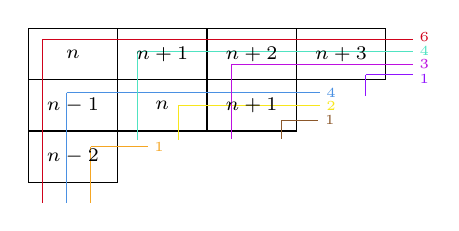
\begin{tikzpicture}[x=0.75pt,y=0.75pt,yscale=-1,xscale=1]
	%uncomment if require: \path (0,91); %set diagram left start at 0, and has height of 91
	
	%Shape: Rectangle [id:dp8815777045687874] 
	\draw   (231,3.2) -- (274.06,3.2) -- (274.06,27.97) -- (231,27.97) -- cycle ;
	%Shape: Rectangle [id:dp5991219333253064] 
	\draw   (274.06,3.2) -- (317.11,3.2) -- (317.11,27.97) -- (274.06,27.97) -- cycle ;
	%Shape: Rectangle [id:dp045704656972568536] 
	\draw   (317.11,3.2) -- (360.17,3.2) -- (360.17,27.97) -- (317.11,27.97) -- cycle ;
	%Shape: Rectangle [id:dp9709748524524378] 
	\draw   (360.17,3.2) -- (403.22,3.2) -- (403.22,27.97) -- (360.17,27.97) -- cycle ;
	%Shape: Rectangle [id:dp2596405378230242] 
	\draw   (231,27.97) -- (274.06,27.97) -- (274.06,52.73) -- (231,52.73) -- cycle ;
	%Shape: Rectangle [id:dp42226610658689956] 
	\draw   (274.06,27.97) -- (317.11,27.97) -- (317.11,52.73) -- (274.06,52.73) -- cycle ;
	%Shape: Rectangle [id:dp4187316025482162] 
	\draw   (317.11,27.97) -- (360.17,27.97) -- (360.17,52.73) -- (317.11,52.73) -- cycle ;
	%Shape: Rectangle [id:dp5305320625060379] 
	\draw   (231,52.73) -- (274.06,52.73) -- (274.06,77.49) -- (231,77.49) -- cycle ;
	%Straight Lines [id:da06952631342029836] 
	\draw [color={rgb, 255:red, 208; green, 2; blue, 27 }  ,draw opacity=1 ]   (237.87,8.48) -- (237.87,87.2) ;
	%Straight Lines [id:da009607264963725326] 
	\draw [color={rgb, 255:red, 208; green, 2; blue, 27 }  ,draw opacity=1 ]   (237.87,8.48) -- (416.31,8.48) ;
	%Straight Lines [id:da7757112780471731] 
	\draw [color={rgb, 255:red, 74; green, 144; blue, 226 }  ,draw opacity=1 ]   (249.46,34.22) -- (249.46,87.2) ;
	%Straight Lines [id:da7936647011909119] 
	\draw [color={rgb, 255:red, 74; green, 144; blue, 226 }  ,draw opacity=1 ]   (249.46,34.22) -- (371.37,34.22) ;
	%Straight Lines [id:da2080337074460996] 
	\draw [color={rgb, 255:red, 245; green, 166; blue, 35 }  ,draw opacity=1 ]   (261.04,60.31) -- (261.04,87.2) ;
	%Straight Lines [id:da1672284401195936] 
	\draw [color={rgb, 255:red, 245; green, 166; blue, 35 }  ,draw opacity=1 ]   (261.04,60.31) -- (288.56,60.31) ;
	%Straight Lines [id:da9072636327703945] 
	\draw [color={rgb, 255:red, 80; green, 227; blue, 194 }  ,draw opacity=1 ]   (283.62,14.27) -- (283.62,56.84) ;
	%Straight Lines [id:da23576145614184396] 
	\draw [color={rgb, 255:red, 80; green, 227; blue, 194 }  ,draw opacity=1 ]   (283.62,14.27) -- (416.31,14.27) ;
	%Straight Lines [id:da13302174297805824] 
	\draw [color={rgb, 255:red, 248; green, 231; blue, 28 }  ,draw opacity=1 ]   (303.31,40.62) -- (303.31,56.84) ;
	%Straight Lines [id:da18353762508780203] 
	\draw [color={rgb, 255:red, 248; green, 231; blue, 28 }  ,draw opacity=1 ]   (303.04,40.62) -- (371.37,40.62) ;
	%Straight Lines [id:da18141605076501444] 
	\draw [color={rgb, 255:red, 139; green, 87; blue, 42 }  ,draw opacity=1 ]   (353.11,47.57) -- (353.11,56.8) ;
	%Straight Lines [id:da4919198143241954] 
	\draw [color={rgb, 255:red, 139; green, 87; blue, 42 }  ,draw opacity=1 ]   (353.11,47.57) -- (370.79,47.57) ;
	%Straight Lines [id:da4333346176137032] 
	\draw [color={rgb, 255:red, 189; green, 16; blue, 224 }  ,draw opacity=1 ]   (328.79,20.64) -- (328.79,56.8) ;
	%Straight Lines [id:da4927197010903921] 
	\draw [color={rgb, 255:red, 189; green, 16; blue, 224 }  ,draw opacity=1 ]   (328.79,20.64) -- (416.31,20.64) ;
	%Straight Lines [id:da1285065636768843] 
	\draw [color={rgb, 255:red, 144; green, 19; blue, 254 }  ,draw opacity=1 ]   (393.65,25.57) -- (393.65,35.99) ;
	%Straight Lines [id:da850577775142418] 
	\draw [color={rgb, 255:red, 144; green, 19; blue, 254 }  ,draw opacity=1 ]   (393.65,25.57) -- (416.31,25.57) ;
	
	
	% Text Node
	\draw (252.53,15.58) node  [font=\scriptsize]  {$n$};
	% Text Node
	\draw (295.58,15.58) node  [font=\scriptsize]  {$n+1$};
	% Text Node
	\draw (252.53,40.35) node  [font=\scriptsize]  {$n-1$};
	% Text Node
	\draw (338.64,15.58) node  [font=\scriptsize]  {$n+2$};
	% Text Node
	\draw (295.58,40.35) node  [font=\scriptsize]  {$n$};
	% Text Node
	\draw (338.64,40.35) node  [font=\scriptsize]  {$n+1$};
	% Text Node
	\draw (381.69,15.58) node  [font=\scriptsize]  {$n+3$};
	% Text Node
	\draw (252.53,65.11) node  [font=\scriptsize]  {$n-2$};
	% Text Node
	\draw (290.56,60.31) node [anchor=west] [inner sep=0.75pt]  [font=\tiny,color={rgb, 255:red, 245; green, 166; blue, 35 }  ,opacity=1 ]  {$1$};
	% Text Node
	\draw (372.79,47.57) node [anchor=west] [inner sep=0.75pt]  [font=\tiny,color={rgb, 255:red, 139; green, 87; blue, 42 }  ,opacity=1 ]  {$1$};
	% Text Node
	\draw (418.31,27.57) node [anchor=west] [inner sep=0.75pt]  [font=\tiny,color={rgb, 255:red, 144; green, 19; blue, 254 }  ,opacity=1 ]  {$1$};
	% Text Node
	\draw (373.37,40.62) node [anchor=west] [inner sep=0.75pt]  [font=\tiny,color={rgb, 255:red, 248; green, 231; blue, 28 }  ,opacity=1 ]  {$2$};
	% Text Node
	\draw (373.37,34.22) node [anchor=west] [inner sep=0.75pt]  [font=\tiny,color={rgb, 255:red, 74; green, 144; blue, 226 }  ,opacity=1 ]  {$4$};
	% Text Node
	\draw (418.31,20.64) node [anchor=west] [inner sep=0.75pt]  [font=\tiny,color={rgb, 255:red, 189; green, 16; blue, 224 }  ,opacity=1 ]  {$3$};
	% Text Node
	\draw (418.31,14) node [anchor=west] [inner sep=0.75pt]  [font=\tiny,color={rgb, 255:red, 80; green, 227; blue, 194 }  ,opacity=1 ]  {$4$};
	% Text Node
	\draw (418.31,7.48) node [anchor=west] [inner sep=0.75pt]  [font=\tiny,color={rgb, 255:red, 208; green, 2; blue, 27 }  ,opacity=1 ]  {$6$};
	
	
\end{tikzpicture}
	\caption{$S_{\boldsymbol{abcdeznt}}$对应的杨图}
	\label{fig:young tablex of S}
\end{figure}

随后我们需要计算所谓的Hook数,考虑一条从每个底部格子下方出发的线,碰到一个格子就右转,总共经过了几个格子,如图中不同颜色的线及其对应颜色所示,而Hook数就是将所有这些数字相乘。那么整个张量的独立分量的个数就是将所有格子中的含$n$表达式相乘,再除以Hook数,例如对于$S_{\boldsymbol{abcdeznt}}$,其Hook数为
\begin{equation*}
	H=\textcolor[rgb]{0.82,0.01,0.11}{6} \times \textcolor[rgb]{0.31,0.89,0.76}{4} \times \textcolor[rgb]{0.74,0.06,0.88}{3} \times \textcolor[rgb]{0.56,0.07,1}{1} \times \textcolor[rgb]{0.29,0.56,0.89}{4} \times \textcolor[rgb]{0.97,0.91,0.11}{2} \times \textcolor[rgb]{0.55,0.34,0.16}{1} \times \textcolor[rgb]{0.96,0.65,0.14}{1} =576,
\end{equation*}
那么其独立分量的个数就为
\begin{equation*}
	\frac{1}{576}( n-2)( n-1) n^{2}( n+1)^{2}( n+2)( n+3) .
\end{equation*}
对于黎曼张量,根据\ref{eq:4.19}可以画出其杨图:

\begin{figure}[h]
	\centering
	

\tikzset{every picture/.style={line width=0.75pt}} %set default line width to 0.75pt        

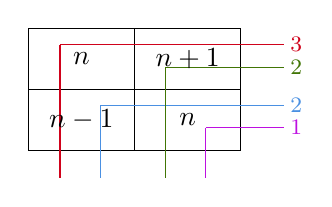
\begin{tikzpicture}[x=0.75pt,y=0.75pt,yscale=-1,xscale=1]
	%uncomment if require: \path (0,91); %set diagram left start at 0, and has height of 91
	
	%Shape: Rectangle [id:dp5303015387664369] 
	\draw   (269,15.2) -- (320.21,15.2) -- (320.21,44.66) -- (269,44.66) -- cycle ;
	%Shape: Rectangle [id:dp5868030307554879] 
	\draw   (320.21,15.2) -- (371.42,15.2) -- (371.42,44.66) -- (320.21,44.66) -- cycle ;
	%Shape: Rectangle [id:dp3019086554132011] 
	\draw   (269,44.66) -- (320.21,44.66) -- (320.21,74.11) -- (269,74.11) -- cycle ;
	%Shape: Rectangle [id:dp2331187580068521] 
	\draw   (320.21,44.66) -- (371.42,44.66) -- (371.42,74.11) -- (320.21,74.11) -- cycle ;
	%Straight Lines [id:da668298705455397] 
	\draw [color={rgb, 255:red, 208; green, 2; blue, 27 }  ,draw opacity=1 ]   (284.31,23.19) -- (284.31,87.52) ;
	%Straight Lines [id:da8368871540410545] 
	\draw [color={rgb, 255:red, 208; green, 2; blue, 27 }  ,draw opacity=1 ]   (284.31,23.19) -- (392.04,23.19) ;
	%Straight Lines [id:da20431247791258755] 
	\draw [color={rgb, 255:red, 74; green, 144; blue, 226 }  ,draw opacity=1 ]   (303.8,52.58) -- (303.8,87.52) ;
	%Straight Lines [id:da9986744066022699] 
	\draw [color={rgb, 255:red, 74; green, 144; blue, 226 }  ,draw opacity=1 ]   (303.8,52.58) -- (391.99,52.58) ;
	%Straight Lines [id:da9192673120152017] 
	\draw [color={rgb, 255:red, 65; green, 117; blue, 5 }  ,draw opacity=1 ]   (334.92,34.14) -- (334.92,87.52) ;
	%Straight Lines [id:da46108143169362115] 
	\draw [color={rgb, 255:red, 65; green, 117; blue, 5 }  ,draw opacity=1 ]   (334.92,34.14) -- (392.04,34.14) ;
	%Straight Lines [id:da40405714240560364] 
	\draw [color={rgb, 255:red, 189; green, 16; blue, 224 }  ,draw opacity=1 ]   (354.53,63.16) -- (354.53,87.56) ;
	%Straight Lines [id:da27807513919607074] 
	\draw [color={rgb, 255:red, 189; green, 16; blue, 224 }  ,draw opacity=1 ]   (354.53,63.16) -- (391.99,63.16) ;
	
	% Text Node
	\draw (294.61,29.93) node  [font=\normalsize]  {$n$};
	% Text Node
	\draw (345.82,29.93) node  [font=\normalsize]  {$n+1$};
	% Text Node
	\draw (294.61,59.38) node  [font=\normalsize]  {$n-1$};
	% Text Node
	\draw (345.82,59.38) node  [font=\normalsize]  {$n$};
	% Text Node
	\draw (393.99,63.16) node [anchor=west] [inner sep=0.75pt]  [font=\footnotesize,color={rgb, 255:red, 189; green, 16; blue, 224 }  ,opacity=1 ]  {$1$};
	% Text Node
	\draw (393.99,52.58) node [anchor=west] [inner sep=0.75pt]  [font=\footnotesize,color={rgb, 255:red, 74; green, 144; blue, 226 }  ,opacity=1 ]  {$2$};
	% Text Node
	\draw (394.04,34.14) node [anchor=west] [inner sep=0.75pt]  [font=\footnotesize,color={rgb, 255:red, 65; green, 117; blue, 5 }  ,opacity=1 ]  {$2$};
	% Text Node
	\draw (394.04,23.19) node [anchor=west] [inner sep=0.75pt]  [font=\footnotesize,color={rgb, 255:red, 208; green, 2; blue, 27 }  ,opacity=1 ]  {$3$};
	
	
\end{tikzpicture}
	\caption{$R_{\boldsymbol{abcd}}$对应的杨图}
	\label{fig:young tablex of R}
\end{figure}

那么其独立分量的个数为
\begin{equation*}
	\frac{1}{3\times 2\times 2} n^{2}( n+1)( n-1) =\frac{1}{12} n^{2} (n^{2} -1).
\end{equation*}
然而,我们谈论的“不可约性”是在$GL( n,\mathbb{C})$的框架下思考的,但如果我们考虑的是$GL( n,\mathbb{C})$的子群,那么可能会需要考虑额外的对称性。例如,我们知道对于洛伦兹群,度规$g_{\boldsymbol{ab}}$是不变量,那么这意味着这些不变量可以将张量进一步约化。最重要的例子就是我们可以将黎曼张量分成三个部分,外尔张量$C_{\boldsymbol{abcd}}$,标量曲率和无迹里奇张量(这被称为里奇分解):
\begin{equation*}
	R\boldsymbol{_{abcd}} =C\boldsymbol{_{abcd}} +E\boldsymbol{_{abcd}} +S\boldsymbol{_{abcd}} ,
\end{equation*}
其中
\begin{equation*}
	S\boldsymbol{_{abcd}} =\frac{2R}{n( n-1)} g_{\boldsymbol{a}[\boldsymbol{d}} g_{\boldsymbol{c}]\boldsymbol{b}} ,E\boldsymbol{_{abcd}} =\frac{4}{n-2} Z_{[\boldsymbol{d} |[\boldsymbol{a}} g_{\boldsymbol{b}] |\boldsymbol{c}]} ,Z_{\boldsymbol{ab}} =R_{\boldsymbol{ab}} -\frac{1}{n} Rg_{\boldsymbol{ab}} .
\end{equation*}
$C_{\boldsymbol{abcd}}$为里奇张量。这样的分解来自于所谓的无迹条件:
\begin{equation*}
	g^{\boldsymbol{ac}} C_{\boldsymbol{abcd}} =0.
\end{equation*}
如果再把洛伦兹群限制为限制性洛伦兹群,那么就会有新的不变量出现,即$e_{\boldsymbol{abcd}}$,推广的对称性会变得更复杂。这里我们考虑一个更简单的情况:
\begin{equation*}
	\phi _{\boldsymbol{ab} \cdots \boldsymbol{f}} =\phi _{\boldsymbol{AB} \cdots \boldsymbol{FA} '\boldsymbol{B} '\cdots \boldsymbol{F} '} =\phi _{(\boldsymbol{AB} \cdots \boldsymbol{F})(\boldsymbol{A} '\boldsymbol{B} '\cdots \boldsymbol{F} ')} ,
\end{equation*}
显然这里我们有
\begin{equation}
	\phi _{\boldsymbol{ab} \cdots \boldsymbol{f}} =\phi _{(\boldsymbol{ab} \cdots \boldsymbol{f})} ,\phi ^{\boldsymbol{a}}{}_{\boldsymbol{ac} \cdots \boldsymbol{f}} =0.
	\label{eq:4.20}
\end{equation}
但如果反过来我们只考虑$\phi _{\boldsymbol{ab} \cdots \boldsymbol{f}} =\phi _{(\boldsymbol{ab} \cdots \boldsymbol{f})}$一个条件,这会给出
\begin{equation*}
	\epsilon ^{\boldsymbol{AB}} \phi _{\boldsymbol{AA} '\boldsymbol{BB} '\boldsymbol{c} \cdots \boldsymbol{f}} =\epsilon ^{\boldsymbol{AB}} \phi _{\boldsymbol{BB 'AA} '\boldsymbol{c} \cdots \boldsymbol{f}} =-\epsilon ^{\boldsymbol{AB}} \phi _{\boldsymbol{AB'BA} '\boldsymbol{c} \cdots \boldsymbol{f}} ,
\end{equation*}
这意味着$\boldsymbol{A} '\boldsymbol{B} '$反对称。但根据第二个条件$\phi ^{\boldsymbol{a}}{}_{\boldsymbol{ac} \cdots \boldsymbol{f}} =0$,这意味着$\phi _{\boldsymbol{AB} \cdots \boldsymbol{FA} '\boldsymbol{B} '\cdots \boldsymbol{F} '}$在$\boldsymbol{AB} ,\boldsymbol{A} '\boldsymbol{B} '$指标上是对称的。因此我们可以看出约束一个张量的条件\ref{eq:4.20}完全等价于一个旋量的对称性。同时,如果一个复张量满足\ref{eq:4.20},我们也可以很简单地计算出复自由变量的个数,如果$\phi _{\boldsymbol{a} \cdots \boldsymbol{f}}$有$r$个指标,那么显然$\phi _{\boldsymbol{A} \cdots \boldsymbol{FA} '\cdots \boldsymbol{F} '}$有$( r+1)^{2}$个独立分量(因为具体指标$A\cdots F$只能取两个值,而对称的条件下只有$r+1$种情况)。同理,我们也可以给出以下定理:

\begin{them}[label={dof of symmetric spinor}]{对称旋量的自由度}
	如果$\varphi _{\boldsymbol{A} \cdots \boldsymbol{CP} '\cdots \boldsymbol{R} '}$是对称的并且其类型为$\{( 0,p) ,( 0,q)\}$,那么它有$( p+1)( q+1)$个(复)独立分量。
\end{them}


\section{旋量操作的张量表示}

我们已经从旋量构造出了张量,那么张量操作很显然可以被看成某些特殊的旋量操作。从这个角度看,部分旋量操作可能没有张量对应,例如单个旋量指标的缩并,或者单个旋量指标的交换。但实际上,本节我们会证明,每一个旋量操作或旋量方程都可以被写成张量操作或张量方程,但有时可能会有一些符号上的模糊性。同时,另一个非常重要的一点是,如果我们把线性旋量方程翻译成张量方程,有可能得到非线性的张量方程。


\subsection{迹反转}

我们首先考虑一些特殊情况。考察任意一个$( 0,2)$型对称张量:
\begin{equation*}
	T_{\boldsymbol{ab}} =T_{\boldsymbol{ba}} ,
\end{equation*}
旋量形式下,我们有:
\begin{equation}
	T_{\boldsymbol{AA} '\boldsymbol{BB} '} =T_{\boldsymbol{BB} '\boldsymbol{AA} '} ,
	\label{eq:4.21}
\end{equation}
这等价于
\begin{equation*}
	T_{\boldsymbol{ABA} '\boldsymbol{B} '} =\frac{1}{2}( T_{\boldsymbol{ABA} '\boldsymbol{B} '} +T_{\boldsymbol{ABB} '\boldsymbol{A} '}) +\frac{1}{2}( T_{\boldsymbol{BAB} '\boldsymbol{A} '} -T_{\boldsymbol{ABB} '\boldsymbol{A} '}) =T_{\boldsymbol{AB}(\boldsymbol{A} '\boldsymbol{B} ')} +T_{[\boldsymbol{BA}]\boldsymbol{B} '\boldsymbol{A} '} ,
\end{equation*}
而根据\ref{eq:4.21},我们知道
\begin{equation*}
	\frac{1}{2}( T_{\boldsymbol{ABA} '\boldsymbol{B} '} +T_{\boldsymbol{ABB} '\boldsymbol{A} '}) =\frac{1}{2}( T_{\boldsymbol{BAB} '\boldsymbol{A} '} +T_{\boldsymbol{ABB} '\boldsymbol{A} '}) =T_{(\boldsymbol{AB})\boldsymbol{A} '\boldsymbol{B} '} ,
\end{equation*}
这意味着
\begin{equation*}
	T_{\boldsymbol{AB}(\boldsymbol{A} '\boldsymbol{B} ')} =T_{(\boldsymbol{AB})\boldsymbol{A} '\boldsymbol{B} '} =T_{(\boldsymbol{AB})(\boldsymbol{A} '\boldsymbol{B} ')} \equiv S_{\boldsymbol{ABA} '\boldsymbol{B} '} .
\end{equation*}
同理,$T_{[\boldsymbol{BA}]\boldsymbol{B} '\boldsymbol{A} '} =T_{[\boldsymbol{BA}][\boldsymbol{B} '\boldsymbol{A} ']}$,利用等式
\begin{equation*}
	\phi _{\mathcal{D}\boldsymbol{AB}} -\phi _{\mathcal{D}\boldsymbol{BA}} =\phi {_{\mathcal{D}\boldsymbol{C}}}^{\boldsymbol{C}} \epsilon _{\boldsymbol{AB}} ,
\end{equation*}
我们可以给出
\begin{equation*}
	T_{\boldsymbol{ab}} =T_{\boldsymbol{AA} '\boldsymbol{BB} '} =S_{\boldsymbol{ABA} '\boldsymbol{B} '} +\epsilon _{\boldsymbol{AB}} \epsilon _{\boldsymbol{A} '\boldsymbol{B} '} \tau ,
\end{equation*}
其中
\begin{equation*}
	\tau =\frac{1}{4} T{_{\boldsymbol{CC} '}}^{\boldsymbol{CC} '} =\frac{1}{4} T{_{\boldsymbol{c}}}^{\boldsymbol{c}} .
\end{equation*}
这意味着我们可以将对称张量分解为
\begin{equation*}
	T_{\boldsymbol{ab}} =S_{\boldsymbol{ab}} +g_{\boldsymbol{ab}} \tau .
\end{equation*}
显然,根据\ref{eq:4.20},$S_{\boldsymbol{ab}}$是对称且无迹的,因此我们称$S_{\boldsymbol{ab}}$为$T_{\boldsymbol{ab}}$的无迹部分:
\begin{equation*}
	S_{\boldsymbol{ab}} =T_{\boldsymbol{ab}} -\frac{1}{4} g_{\boldsymbol{ab}} T{_{\boldsymbol{c}}}^{\boldsymbol{c}} .
\end{equation*}
我们称这样的操作为\textbf{迹反转}(trace reversal):
\begin{equation*}
	\hat{T}_{\boldsymbol{ab}} \equiv T_{\boldsymbol{ab}} -\frac{1}{2} g_{\boldsymbol{ab}} T{_{\boldsymbol{c}}}^{\boldsymbol{c}} ,
\end{equation*}
那么
\begin{equation*}
	\hat{T}{_{\boldsymbol{c}}}^{\boldsymbol{c}} =T{_{\boldsymbol{c}}}^{\boldsymbol{c}} -\frac{1}{2} g_{\boldsymbol{ab}} g^{\boldsymbol{ab}} T{_{\boldsymbol{c}}}^{\boldsymbol{c}} =-T{_{\boldsymbol{c}}}^{\boldsymbol{c}} .
\end{equation*}
在旋量形式中:
\begin{equation*}
	\begin{aligned}
		\hat{T}_{\boldsymbol{ab}} =\hat{T}_{\boldsymbol{AA} '\boldsymbol{BB} '} & =S_{\boldsymbol{ABA} '\boldsymbol{B} '} -\epsilon _{\boldsymbol{AB}} \epsilon _{\boldsymbol{A} '\boldsymbol{B} '} \tau \\
		& =S_{\boldsymbol{BAA} '\boldsymbol{B} '} +\epsilon _{\boldsymbol{BA}} \epsilon _{\boldsymbol{A} '\boldsymbol{B} '} \tau =T_{\boldsymbol{BAA} '\boldsymbol{B} '} =T_{\boldsymbol{ABB} '\boldsymbol{A} '} ,
	\end{aligned}
\end{equation*}
这意味着某两个旋量指标交换位置等价于(对称)张量上的迹反转操作。


\subsection{对偶化}

现在考虑任意一个反对称的$( 0,2)$类的世界张量,有时候也被称为双矢(bivector):
\begin{equation*}
	F_{\boldsymbol{ab}} =-F_{\boldsymbol{ba}} ,
\end{equation*}
旋量形式中这意味着
\begin{equation*}
	F_{\boldsymbol{AA} '\boldsymbol{BB} '} =-F_{\boldsymbol{BB} '\boldsymbol{AA} '} ,
\end{equation*}
这意味着
\begin{equation}
	F_{\boldsymbol{ABA} '\boldsymbol{B} '} =\frac{1}{2}( F_{\boldsymbol{ABA} '\boldsymbol{B} '} -T_{\boldsymbol{ABB} '\boldsymbol{A} '}) +\frac{1}{2}( F_{\boldsymbol{ABB} '\boldsymbol{A} '} -F_{\boldsymbol{BAB} '\boldsymbol{A} '}) =\phi _{\boldsymbol{AB}} \epsilon _{\boldsymbol{A'B} '} +\epsilon _{\boldsymbol{AB}} \psi _{\boldsymbol{A} '\boldsymbol{B} '} ,
	\label{eq:4.22}
\end{equation}
其中
\begin{equation*}
	\phi _{\boldsymbol{AB}} =\phi _{(\boldsymbol{AB})} =\frac{1}{2} F{_{\boldsymbol{ABC} '}}^{\boldsymbol{C} '} ,\psi _{\boldsymbol{A} '\boldsymbol{B} '} =\psi _{(\boldsymbol{A} '\boldsymbol{B} ')} =\frac{1}{2} F{_{\boldsymbol{C}}}^{\boldsymbol{C}}{}_{\boldsymbol{A} '\boldsymbol{B} '} .
\end{equation*}
如果对\ref{eq:4.22}取复共轭,我们有
\begin{equation*}
	\overline{F}_{\boldsymbol{ab}} =\overline{F}_{\boldsymbol{A} '\boldsymbol{B} '\boldsymbol{AB}} =\overline{\phi }_{\boldsymbol{A} '\boldsymbol{B} '} \epsilon _{\boldsymbol{AB}} +\epsilon _{\boldsymbol{A} '\boldsymbol{B} '}\overline{\psi }_{\boldsymbol{AB}} ,
\end{equation*}
这意味着复共轭操作$F_{\boldsymbol{ab}} \mapsto \overline{F}_{\boldsymbol{ab}}$对应$\psi _{\boldsymbol{A} '\boldsymbol{B} '} \mapsto \overline{\phi }_{\boldsymbol{A} '\boldsymbol{B} '}$。那么如果$F_{\boldsymbol{ab}}$是实的,这意味着$\psi _{\boldsymbol{A} '\boldsymbol{B} '} =\overline{\phi }_{\boldsymbol{A} '\boldsymbol{B} '}$,或
\begin{equation}
	F_{\boldsymbol{ab}} =\phi _{\boldsymbol{AB}} \epsilon _{\boldsymbol{A'B} '} +\epsilon _{\boldsymbol{AB}}\overline{\phi }_{\boldsymbol{A} '\boldsymbol{B} '} ,
	\label{eq:4.23}
\end{equation}
这意味着实反对称$F_{\boldsymbol{ab}}$与对称旋量$\phi _{\boldsymbol{AB}}$有一一对应关系。



现在我们定义$F_{\boldsymbol{ab}}$的对偶$\prescript{*}{}{} F_{\boldsymbol{ab}}$为
\begin{equation*}
	\prescript{*}{}{} F_{\boldsymbol{ab}} =\frac{1}{2} e_{\boldsymbol{abcd}} F^{\boldsymbol{cd}} =\frac{1}{2} e{_{\boldsymbol{ab}}}^{\boldsymbol{cd}} F_{\boldsymbol{cd}} .
\end{equation*}
那么如果我们将$e_{\boldsymbol{abcd}}$的定义\ref{eq:4.16}带入\ref{eq:4.22},可以给出
\begin{equation}
	\prescript{*}{}{} F_{\boldsymbol{ab}} =\prescript{*}{}{} F_{\boldsymbol{ABA} '\boldsymbol{B} '} =-\mathrm{i} \phi _{\boldsymbol{AB}} \epsilon _{\boldsymbol{A} '\boldsymbol{B} '} +\mathrm{i} \epsilon _{\boldsymbol{AB}} \psi _{\boldsymbol{A} '\boldsymbol{B} '} ,
	\label{eq:4.24}
\end{equation}
即
\begin{equation*}
	\prescript{*}{}{} F_{\boldsymbol{ABA} '\boldsymbol{B} '} =\mathrm{i} F_{\boldsymbol{ABB} '\boldsymbol{A} '} =-\mathrm{i} F_{\boldsymbol{BAA} '\boldsymbol{B} '} ,
\end{equation*}
这意味着对于反对称张量,旋量指标的置换等于将其代换成$\pm \mathrm{i}$乘其对偶$\prescript{*}{}{} F$!那么将指标置换两次,自然得到
\begin{equation*}
	\prescript{**}{}{} F_{\boldsymbol{ab}} =F_{\boldsymbol{ba}} =-F_{\boldsymbol{ab}} .
\end{equation*}
考虑更一般的情况,对于一个大张量中的两个反对称指标取对偶:
\begin{equation*}
	\prescript{*}{}{} G_{\boldsymbol{ab}\mathcal{A}} \equiv \frac{1}{2} e{_{\boldsymbol{ab}}}^{\boldsymbol{cd}} G_{\boldsymbol{cd}\mathcal{A}} ,G_{\boldsymbol{ab}\mathcal{A}} =G_{[\boldsymbol{ab}]\mathcal{A}} .
\end{equation*}
我们给出一个有用的引理:
\begin{equation}
	\prescript{*}{}{} G_{[\boldsymbol{abc}]\mathcal{A}} =0\Leftrightarrow \prescript{*}{}{} G^{\boldsymbol{ab}}{}_{\boldsymbol{a}\mathcal{A}} =0.
	\label{eq:4.25}
\end{equation}
要证明这个只需注意到
\begin{equation*}
	G_{[\boldsymbol{abc}]\mathcal{A}} =g{_{[\boldsymbol{a}}}^{\boldsymbol{p}} g{_{\boldsymbol{b}}}^{\boldsymbol{q}} g{_{\boldsymbol{c}]}}^{\boldsymbol{r}} G_{\boldsymbol{pqr}\mathcal{A}} =-\frac{1}{6} e_{\boldsymbol{abcd}} e^{\boldsymbol{pqrd}} G_{\boldsymbol{pqr}\mathcal{A}} =\frac{1}{3} e_{\boldsymbol{abcd}}\prescript{*}{}{} G^{\boldsymbol{pd}}{}_{\boldsymbol{p}\mathcal{A}} ,
\end{equation*}
因此如果$\prescript{*}{}{} G^{\boldsymbol{pd}}{}_{\boldsymbol{p}\mathcal{A}} =0\Rightarrow G_{[\boldsymbol{abc}]\mathcal{A}} \Rightarrow \prescript{*}{}{} G_{[\boldsymbol{abc}]\mathcal{A}} =0$。反过来,注意到
\begin{equation*}
	\begin{aligned}
		& \prescript{*}{}{} G^{\boldsymbol{ab}}{}_{\boldsymbol{f}\mathcal{A}} =\frac{1}{2} e^{\boldsymbol{abcd}} G_{\boldsymbol{cdf}\mathcal{B}} =\frac{1}{2} e^{\boldsymbol{abcd}} G_{[\boldsymbol{fcd}]\mathcal{A}}\\
		\Rightarrow  & \prescript{*}{}{} G_{[\boldsymbol{abf}]\mathcal{A}} =\frac{1}{2} e{_{\boldsymbol{ab}}}^{\boldsymbol{cd}} G_{[\boldsymbol{fcd}]\mathcal{A}} =0\\
		\Rightarrow  & \prescript{*}{}{} G^{\boldsymbol{ab}}{}_{\boldsymbol{f}\mathcal{A}} =0.
	\end{aligned}
\end{equation*}
对于一个指标或者三个指标反对称的情况,也可以构造对偶:
\begin{equation*}
	\prescript{\dagger }{}{} J_{\boldsymbol{abc}\mathcal{A}} \equiv e{_{\boldsymbol{abc}}}^{\boldsymbol{d}} J_{\boldsymbol{d}\mathcal{A}} ,\prescript{\ddagger }{}{} K_{\boldsymbol{a}\mathcal{B}} \equiv \frac{1}{6} e{_{\boldsymbol{a}}}^{\boldsymbol{bcd}} K_{\boldsymbol{bcd}\mathcal{B}} ,
\end{equation*}
容易证明
\begin{equation*}
	\prescript{\dagger \ddagger }{}{} J_{\boldsymbol{a}\mathcal{A}} =J_{\boldsymbol{a}\mathcal{A}} ,\prescript{\ddagger \dagger }{}{} K_{\boldsymbol{abc}\mathcal{B}} =K_{\boldsymbol{abc}\mathcal{B}} .
\end{equation*}
如果将$\mathcal{A}$换为$\boldsymbol{d}\mathcal{C}$,将$\mathcal{B}$换位$\boldsymbol{d}\mathcal{D}$,我们容易证明
\begin{equation*}
	\prescript{\dagger }{}{} J_{[\boldsymbol{abcd}]\mathcal{C}} =\frac{1}{4} e_{\boldsymbol{abcd}} J{_{\boldsymbol{f}}}^{\boldsymbol{f}}{}_{\mathcal{C}} ,K_{[\boldsymbol{abcd}]\mathcal{D}} =\frac{1}{4} e_{\boldsymbol{abcd}}\prescript{\ddagger }{}{} K{_{\boldsymbol{f}}}^{\boldsymbol{f}}{}_{\mathcal{D}} .
\end{equation*}
旋量形式中,我们带入直接带入$e$的定义可以给出
\begin{equation*}
	\begin{aligned}
		\prescript{\dagger }{}{} J_{\boldsymbol{abc}\mathcal{A}} & =\mathrm{i} \epsilon _{\boldsymbol{AC}} \epsilon _{\boldsymbol{B} '\boldsymbol{C} '} J_{\boldsymbol{BA} '\mathcal{A}} -\mathrm{i} \epsilon _{\boldsymbol{BC}} \epsilon _{\boldsymbol{A} '\boldsymbol{C} '} J_{\boldsymbol{AB} '\mathcal{A}} ,\\
		\prescript{\ddagger }{}{} K_{\boldsymbol{a}\mathcal{B}} & =\frac{\mathrm{i}}{3} K{_{\boldsymbol{AB} '\boldsymbol{BA} '}}^{\boldsymbol{BB} '}{}_{\mathcal{B}} .
	\end{aligned}
\end{equation*}
现在我们回到$F_{\boldsymbol{ab}}$。考虑两种情况:
\begin{enumerate}[label=(\alph*)]
	\item $\prescript{*}{}{} F_{\boldsymbol{ab}} =-\mathrm{i} F_{\boldsymbol{ab}}$,等价于$F_{\boldsymbol{ABA} '\boldsymbol{B} '} =F_{\boldsymbol{BAA} '\boldsymbol{B} '} =-F_{\boldsymbol{ABB} '\boldsymbol{A} '}$,即$F_{\boldsymbol{ABA} '\boldsymbol{B} '} =F_{(\boldsymbol{AB})[\boldsymbol{A} '\boldsymbol{B} ']}$。我们称这种情况为自对偶的。
	\item $\prescript{*}{}{} F_{\boldsymbol{ab}} =\mathrm{i} F_{\boldsymbol{ab}}$,等价于$F_{\boldsymbol{ABA} '\boldsymbol{B} '} =-F_{\boldsymbol{BAA} '\boldsymbol{B} '} =F_{\boldsymbol{ABB} '\boldsymbol{A} '}$,即$F_{\boldsymbol{ABA} '\boldsymbol{B} '} =F_{[\boldsymbol{AB}](\boldsymbol{A} '\boldsymbol{B} ')}$。我们称这种情况为反自对偶的。
\end{enumerate}

我们从\ref{eq:4.22},\ref{eq:4.24}中可以给出,任何一个反对称张量都可以被分解为:
\begin{equation*}
	F_{\boldsymbol{ab}} =\prescript{-}{}{} F_{\boldsymbol{ab}} +\prescript{+}{}{} F_{\boldsymbol{ab}}
\end{equation*}
其中
\begin{equation*}
	\begin{aligned}
		\prescript{-}{}{} F_{\boldsymbol{ab}} & \equiv \frac{1}{2} (F_{\boldsymbol{ab}} +\mathrm{i}\prescript{*}{}{} F_{\boldsymbol{ab}} )=\phi _{\boldsymbol{AB}} \epsilon _{\boldsymbol{A'B} '}\\
		\prescript{+}{}{} F_{\boldsymbol{ab}} & \equiv \frac{1}{2} (F_{\boldsymbol{ab}} -\mathrm{i}\prescript{*}{}{} F_{\boldsymbol{ab}} )=\epsilon _{\boldsymbol{AB}} \psi _{\boldsymbol{A} '\boldsymbol{B} '} ,
	\end{aligned}
\end{equation*}
而$\prescript{-}{}{} F$是反自对偶的,$\prescript{+}{}{} F$是自对偶的。



如果将对偶操作推广,可得到操作\textbf{对偶性旋转}(duality rotation),$F_{\boldsymbol{ab}} \mapsto \prescript{( \theta )}{}{} F_{\boldsymbol{ab}}$,定义为
\begin{equation*}
	\prescript{( \theta )}{}{} F_{\boldsymbol{ab}} \equiv F_{\boldsymbol{ab}}\cos \theta +\prescript{*}{}{} F_{\boldsymbol{ab}}\sin \theta =\prescript{-}{}{} F_{\boldsymbol{ab}}\mathrm{e}^{-\mathrm{i} \theta } +\prescript{+}{}{} F_{\boldsymbol{ab}}\mathrm{e}^{\mathrm{i} \theta } =\mathrm{e}^{-\mathrm{i} \theta } \phi _{\boldsymbol{AB}} \epsilon _{\boldsymbol{A} '\boldsymbol{B} '} +\mathrm{e}^{\mathrm{i} \theta } \epsilon _{\boldsymbol{AB}} \psi _{\boldsymbol{A} '\boldsymbol{B} '} .
\end{equation*}


我们可以用旋量证明许多(反)自对偶矢量的性质,例如对于任意两个张量$F,G$,都有
\begin{equation*}
	\prescript{-}{}{} F_{\boldsymbol{ab}}\prescript{+}{}{} G^{\boldsymbol{ab}} =0,\prescript{-}{}{} F{_{\boldsymbol{a}}}^{\boldsymbol{b}}\prescript{+}{}{} G_{\boldsymbol{bc}} =\prescript{+}{}{} G{_{\boldsymbol{a}}}^{\boldsymbol{b}}\prescript{-}{}{} F_{\boldsymbol{bc}} .
\end{equation*}
只需要带入计算即可,但是后者对于张量方法证明则较为麻烦。


\subsection{一般转换流程}

我们已经看到,对于一个对称张量,交换其旋量指标等价于将其变换成迹反转,而对于一个反对称张量,交换其旋量指标等价于将其变换成对偶,那么对于一个一般的$( 0,2)$型张量$H_{\boldsymbol{ab}}$,我们知道
\begin{equation*}
	H_{\boldsymbol{AA} '\boldsymbol{BB} '} =H_{(\boldsymbol{ab})} +H_{[\boldsymbol{ab}]} ,
\end{equation*}
那么交换指标给出
\begin{equation*}
	\begin{aligned}
		H_{\boldsymbol{BAA} '\boldsymbol{B} '} & =\hat{H}_{(\boldsymbol{ab})} +\mathrm{i}\prescript{*}{}{} H_{[\boldsymbol{ab}]} =\frac{1}{2} (H_{\boldsymbol{ab}} +H_{\boldsymbol{ba}} -H{_{\boldsymbol{c}}}^{\boldsymbol{c}} g_{\boldsymbol{ab}} +\mathrm{i} e_{\boldsymbol{abcd}} H^{\boldsymbol{cd}} ),\\
		H_{\boldsymbol{ABB} '\boldsymbol{A} '} & =\hat{H}_{(\boldsymbol{ab})} -\mathrm{i}\prescript{*}{}{} H_{[\boldsymbol{ab}]} =\frac{1}{2} (H_{\boldsymbol{ab}} +H_{\boldsymbol{ba}} -H{_{\boldsymbol{c}}}^{\boldsymbol{c}} g_{\boldsymbol{ab}} -\mathrm{i} e_{\boldsymbol{abcd}} H^{\boldsymbol{cd}} ).
	\end{aligned}
\end{equation*}
由于交换旋量指标完全可以通过旋量度规升降指标实现,这意味着我们也可以构造一个算符完成这件事。一个自然的构造是
\begin{equation*}
	\begin{aligned}
		U{_{\boldsymbol{ab}}}^{\boldsymbol{cd}} & =\epsilon {_{\boldsymbol{A}}}^{\boldsymbol{D}} \epsilon {_{\boldsymbol{B}}}^{\boldsymbol{C}} \epsilon {_{\boldsymbol{A} '}}^{\boldsymbol{C} '} \epsilon {_{\boldsymbol{B} '}}^{\boldsymbol{D} '}\\
		& =\frac{1}{2} (g{_{\boldsymbol{a}}}^{\boldsymbol{c}} g{_{\boldsymbol{b}}}^{\boldsymbol{d}} +g{_{\boldsymbol{a}}}^{\boldsymbol{d}} g{_{\boldsymbol{b}}}^{\boldsymbol{c}} -g_{\boldsymbol{ab}} g^{\boldsymbol{cd}} +\mathrm{i} e{_{\boldsymbol{ab}}}^{\boldsymbol{cd}} ),
	\end{aligned}
\end{equation*}
那么旋量指标的交换自然为
\begin{equation*}
	H_{\boldsymbol{BAA} '\boldsymbol{B} '} =U{_{\boldsymbol{ab}}}^{\boldsymbol{cd}} H_{\boldsymbol{cd}} ,H_{\boldsymbol{ABB} '\boldsymbol{A} '} =\overline{U}{_{\boldsymbol{ab}}}^{\boldsymbol{cd}} H_{\boldsymbol{cd}} .
\end{equation*}
同时注意到
\begin{equation*}
	U^{\boldsymbol{ab}}{}_{\boldsymbol{cd}} =U{_{\boldsymbol{cd}}}^{\boldsymbol{ab}} ,U{_{\boldsymbol{ba}}}^{\boldsymbol{cd}} =\overline{U}{_{\boldsymbol{ab}}}^{\boldsymbol{cd}} =U{_{\boldsymbol{ab}}}^{\boldsymbol{dc}} ,
\end{equation*}
那么我们可以写出
\begin{equation*}
	H^{\boldsymbol{BAA} '\boldsymbol{B} '} =U{_{\boldsymbol{cd}}}^{\boldsymbol{ab}} H^{\boldsymbol{cd}} ,H_{\boldsymbol{ABB} '\boldsymbol{A} '} =U{_{\boldsymbol{ba}}}^{\boldsymbol{cd}} H_{\boldsymbol{cd}} .
\end{equation*}
因此,用这个算符$U$我们可以将\textbf{任何}旋量指标替换变成旋量形式,因为任何指标代换可以被写成旋量指标交换的复合。



最后我们讨论如何将一个一般的旋量$\chi _{\mathcal{A}} =\chi _{\boldsymbol{A} \cdots \boldsymbol{EB} '\cdots \boldsymbol{F} '}$给出其张量实现。我们分为三种情况:
\begin{itemize}
	\item 如果带撇与不带撇的指标数一样,那么我们只需要使用指标替换操作,将带撇的指标替换成与不带撇的指标一样的指标,给出其张量版本。但我们知道,指标替换的方式不止一种,例如我们可以让$\chi _{\boldsymbol{ABCD} '\boldsymbol{E} '\boldsymbol{F} '} \mapsto \chi _{\boldsymbol{ABCA} '\boldsymbol{B} '\boldsymbol{C} '}$,但也可以将其换为$\chi _{\boldsymbol{ABCB} '\boldsymbol{A} '\boldsymbol{C} '}$,或$\chi _{\boldsymbol{EBDB} '\boldsymbol{E} '\boldsymbol{D} '}$。然而我们知道,这样做的区别仅仅在于旋量指标的位置有置换,而这对应于相应的张量算符$U$,因此我们只需要选择其中一个,其他张量实现都与选择的张量相差一个张量变换。
	\item 如果旋量指标的总数是偶数,即使带撇和不带撇的指标数可能不一样。那么这种情况,我们只需要将其乘以$\epsilon $张量,将不足的指标补齐,便可回到第一种情况,并且这样做也没有添加任何信息。例如对于旋量$\psi _{\boldsymbol{AB}} ,\phi _{\boldsymbol{AB} '\boldsymbol{C} '\boldsymbol{D} '}$,我们可以将其张量实现选为$P_{\boldsymbol{ab}} =\psi _{\boldsymbol{AB}} \epsilon _{\boldsymbol{A} '\boldsymbol{B} '}$,以及$Q_{\boldsymbol{abc}} =\phi _{\boldsymbol{AA} '\boldsymbol{B} '\boldsymbol{C} '} \epsilon _{\boldsymbol{BC}}$。
	\item 如果旋量指标的总数是奇数,这种情况无法完全用张量实现,可能会有一个符号的不确定性。接受了这点,我们只需要用$\chi _{\mathcal{A}_{1}} \chi _{\mathcal{A}_{2}}$,这样就能将$\chi _{\mathcal{A}}$确定到一个符号的差距。例如对于旋量$\kappa _{\boldsymbol{A}}$,我们首先将其“平方”得到$\kappa _{\boldsymbol{A}} \kappa _{\boldsymbol{B}}$,随后乘以$\epsilon _{\boldsymbol{A} '\boldsymbol{B} '}$。为了几何上的实现方便,我们可以构造$P_{\boldsymbol{ab}} =\kappa _{\boldsymbol{A}} \kappa _{\boldsymbol{B}} \epsilon _{\boldsymbol{A} '\boldsymbol{B} '} +\epsilon _{\boldsymbol{AB}}\overline{\kappa }_{\boldsymbol{A} '}\overline{\kappa }_{\boldsymbol{B} '}$。实际上,这就是我们之前给出的\ref{eq:4.13}。
\end{itemize}


\section{流形上某点的张量和旋量*}

本节我们给出一些对于在流形上某点的旋量成立的结论,这意味着这些结论可能对于流形上的旋量场并不成立。有些定理我们不会给出证明,仅仅罗列结论。

\begin{them}[label={them:3.5}]{}
	如果$\psi _{\mathcal{A}} \phi _{\mathcal{B}} =\chi _{\mathcal{A}} \theta _{\mathcal{B}} \neq 0$,那么$\psi _{\mathcal{A}} =\kappa \chi _{\mathcal{A}}$,且$\phi _{\mathcal{B}} =\kappa ^{-1} \theta _{\mathcal{B}}$,其中$\kappa \in \mathfrak{S}$非零。
\end{them}

\begin{proof}
	选取一个$\xi ^{\mathcal{B}}$在等式两边缩并给出$\psi _{\mathcal{A}} \phi _{\mathcal{B}} \xi ^{\mathcal{B}} =\chi _{\mathcal{A}} \theta _{\mathcal{B}} \xi ^{\mathcal{B}}$,选取$\xi $令$\lambda \equiv \phi _{\mathcal{B}} \xi ^{\mathcal{B}} \neq 0$,那么我们知道
	\begin{equation*}
		\psi _{\mathcal{A}} =\kappa \chi _{\mathcal{A}} ,\kappa =\lambda ^{-1} \theta _{\mathcal{B}} \xi ^{\mathcal{B}} .
	\end{equation*}
	同理$\phi _{\mathcal{B}} =\kappa ^{-1} \theta _{\mathcal{B}}$。
\end{proof}

\begin{them}[label={them:3.6}]{}
	如果$\psi _{\mathcal{AB}} \phi _{\mathcal{CD}} =\chi _{\mathcal{AD}} \theta _{\mathcal{CB}} \neq 0$,那么存在$\alpha _{\mathcal{A}} ,\beta _{\mathcal{B}} ,\gamma _{\mathcal{C}} ,\rho _{\mathcal{D}}$,使得
	\begin{equation*}
		\psi _{\mathcal{AB}} =\alpha _{\mathcal{A}} \beta _{\mathcal{B}} ,\phi _{\mathcal{CD}} =\gamma _{\mathcal{C}} \rho _{\mathcal{D}} ,\chi _{\mathcal{AD}} =\alpha _{\mathcal{A}} \rho _{\mathcal{D}} ,\theta _{\mathcal{CB}} =\gamma _{\mathcal{C}} \beta _{\mathcal{B}} .
	\end{equation*}
\end{them}

\begin{proof}
	思路同上,选取$\xi ^{\mathcal{C}} ,\eta ^{\mathcal{D}}$令$\lambda \equiv \xi ^{\mathcal{C}} \eta ^{\mathcal{D}} \phi _{\mathcal{CD}} \neq 0$,那么两边取内积给出$\psi _{\mathcal{AB}} \lambda =(\chi _{\mathcal{AD}} \eta ^{\mathcal{D}} )(\xi ^{\mathcal{C}} \theta _{\mathcal{CB}} )$。只需令$\alpha _{\mathcal{A}} =\lambda ^{-1} \chi _{\mathcal{AD}} \eta ^{\mathcal{D}}$,$\beta _{\mathcal{B}} =\xi ^{\mathcal{C}} \theta _{\mathcal{CB}}$,那么我们有$\psi _{\mathcal{AB}} =\alpha _{\mathcal{A}} \beta _{\mathcal{B}}$。同理可得其他部分。
\end{proof}

作为上述定理的一个特殊情况,我们看到如果$\psi _{[\mathcal{A}_{1}} \phi _{\mathcal{A}_{2}]} =0$,那么$\psi _{\mathcal{A}} =\kappa \phi _{\mathcal{A}}$或$\phi _{\mathcal{A}} =0$。

\begin{them}[label={them:3.7}]{}
	对于$\lambda {_{\mathcal{AB}}}^{\mathcal{Q}}$,以下三个条件等价:
	\begin{enumerate}[label=(\alph*)]
		\item $\lambda {_{\mathcal{AB}}}^{\mathcal{Q}} \xi _{\mathcal{Q}}$对于每一个$\xi _{\mathcal{Q}} \in \mathfrak{S}_{\mathcal{Q}}$可以写成$\rho _{\mathcal{A}} \zeta _{\mathcal{B}}$的形式。
		\item $\lambda {_{\mathcal{A}_{1}[\mathcal{B}_{1}}}^{(\mathcal{Q}_{1}} \lambda {_{|\mathcal{A}_{2} |\mathcal{B}_{2}]}}^{\mathcal{Q}_{2})} =0$。
		\item $\lambda {_{\mathcal{AB}}}^{\mathcal{Q}}$可以被写成要么$\alpha _{\mathcal{A}} \phi {_{\mathcal{B}}}^{\mathcal{Q}}$的形式,要么$\theta {_{\mathcal{B}}}^{\mathcal{Q}} \beta _{\mathcal{A}}$的形式。
	\end{enumerate}
\end{them}

这个定理的证明只需将$\lambda {_{\mathcal{A}_{1}[\mathcal{B}_{1}}}^{(\mathcal{Q}_{1}} \lambda {_{|\mathcal{A}_{2} |\mathcal{B}_{2}]}}^{\mathcal{Q}_{2})} =0$展开,并适当缩并即可。

\begin{them}[label={them:3.8}]{}
	$\psi {_{(\mathcal{A}_{1} \cdots \mathcal{A}_{r}}}^{\mathcal{B}} \phi {_{\mathcal{A}_{r+1} \cdots \mathcal{A}_{r+s})}}^{\mathcal{C}} =0$意味着要么$\psi {_{(\mathcal{A}_{1} \cdots \mathcal{A}_{r})}}^{\mathcal{B}} =0$,要么$\phi {_{(\mathcal{A}_{1} \cdots \mathcal{A}_{s})}}^{\mathcal{C}} =0$。
\end{them}

\begin{proof}
	只需要考虑$\psi {_{\mathcal{A}_{1} \cdots \mathcal{A}_{r}}}^{\mathcal{B}} \xi ^{\mathcal{A}_{1}} \cdots \xi ^{\mathcal{A}_{r}} \phi {_{\mathcal{A}_{r+1} \cdots \mathcal{A}_{r+s}}}^{\mathcal{C}} \xi ^{\mathcal{A}_{r+1}} \cdots \xi ^{\mathcal{A}_{r+s}}$,随后使用\ref{them:zero symmetric spinor}以及\ref{them:3.5}即可证明。
\end{proof}


以上结果对于任意维度都适用,但对于二维的旋量空间,有些特殊的结论,例如根据\ref{them:3.6},我们知道如果$\psi _{\mathcal{A}\boldsymbol{B}} ,\theta _{\mathcal{C}\boldsymbol{B}} \neq 0$,那么$\psi {_{\mathcal{A}}}^{\boldsymbol{B}} \theta _{\mathcal{C}\boldsymbol{B}} =0$可以推出$\psi _{\mathcal{A}\boldsymbol{B}} =\alpha _{\mathcal{A}} \beta _{\boldsymbol{B}} ,\theta _{\mathcal{C}\boldsymbol{B}} =\gamma _{\mathcal{C}} \beta _{\boldsymbol{B}}$。


\subsection{主类光方向}

下面的结果除了用了自旋空间的二维性,还使用了$\mathfrak{S}$作为复数的可除环是代数上封闭的这个条件。

\begin{them}[label={them:3.9}]{}
	如果$\phi _{\boldsymbol{AB} \cdots \boldsymbol{L}} =\phi _{(\boldsymbol{AB} \cdots \boldsymbol{L})} \neq 0$,那么存在$\alpha _{\boldsymbol{A}} ,\beta _{\boldsymbol{A}} ,\cdots ,\lambda _{\boldsymbol{A}} \in \mathfrak{S}_{\boldsymbol{A}}$满足
	\begin{equation}
		\phi _{\boldsymbol{AB} \cdots \boldsymbol{L}} =\alpha _{(\boldsymbol{A}} \beta _{\boldsymbol{B}} \cdots \lambda _{\boldsymbol{L})} ,
		\label{eq:4.26}
	\end{equation}
	且这个分解在相差一个系数的意义上是唯一的。
\end{them}

\begin{proof}
	选取一个自旋标架:$o^{\boldsymbol{A}} ,\iota ^{\boldsymbol{A}}$,在这个标架下满足$\phi _{111\cdots 1} \neq 0$。同时选取一个$\xi ^{\boldsymbol{A}} \in \mathfrak{S}^{\boldsymbol{A}}$,满足在这个标架下的分量为$(\xi ^{0} ,\xi ^{1} )=( 1,z)$,那么如果$\phi $有$n$个自旋指标,我们知道
	\begin{equation*}
		\phi _{\boldsymbol{AB} \cdots \boldsymbol{L}} \xi ^{\boldsymbol{A}} \xi ^{\boldsymbol{B}} \cdots \xi ^{\boldsymbol{L}} =\phi _{00\cdots 0} +nz\phi _{10\cdots 0} +\cdots +z^{n} \phi _{11\cdots 1} ,
	\end{equation*}
	根据代数学基本定理,上述多项式一定有一个在相差常数的意义下有一个唯一的分解:
	\begin{equation*}
		\phi _{\boldsymbol{AB} \cdots \boldsymbol{L}} \xi ^{\boldsymbol{A}} \xi ^{\boldsymbol{B}} \cdots \xi ^{\boldsymbol{L}} =(\alpha _{0} +z\alpha _{1} )(\beta _{0} +z\beta _{1} )\cdots (\lambda _{0} +z\lambda _{1} ),
	\end{equation*}
	那么我们令$\alpha _{\boldsymbol{A}} =(\alpha ^{0} ,\alpha ^{1} )$,那么我们知道$\alpha _{0} +z\alpha _{1} =\alpha _{A} \xi ^{A} =\alpha _{\boldsymbol{A}} \xi ^{\boldsymbol{A}}$,从而
	\begin{equation*}
		\phi _{\boldsymbol{AB} \cdots \boldsymbol{L}} \xi ^{\boldsymbol{A}} \xi ^{\boldsymbol{B}} \cdots \xi ^{\boldsymbol{L}} =(\alpha _{\boldsymbol{A}} \xi ^{\boldsymbol{A}} )(\beta _{\boldsymbol{B}} \xi ^{\boldsymbol{B}} )\cdots (\lambda _{\boldsymbol{L}} \xi ^{\boldsymbol{L}} ),
	\end{equation*}
	因此
	\begin{equation*}
		\{\phi _{\boldsymbol{AB} \cdots \boldsymbol{L}} -\alpha _{(\boldsymbol{A}} \beta _{\boldsymbol{B}} \cdots \lambda _{\boldsymbol{L})}\} \xi ^{\boldsymbol{A}} \xi ^{\boldsymbol{B}} \cdots \xi ^{\boldsymbol{L}} =0.
	\end{equation*}
	根据\ref{them:zero symmetric spinor},我们知道有式\ref{eq:4.26}。
\end{proof}


我们将这种把对称张量分解的方法叫做\textbf{正则分解}(canonical decomposition),其中这样构造出的旋量$\alpha _{\boldsymbol{A}} ,\beta _{\boldsymbol{A}} ,\cdots ,\lambda _{\boldsymbol{L}}$被称为\textbf{主旋量}(principal spinor)。我们知道一个旗杆$K^{\boldsymbol{a}} =\kappa ^{\boldsymbol{A}}\overline{\kappa }^{\boldsymbol{A} '}$对应了很多不同的主旋量,我们称这样的方向为\textbf{主类光方向}(principal null directions, PND),其对应类光矢量被称为\textbf{主类光矢量}(principal null vectors)。因此,每一个对称的$n$指标旋量唯一地定义了$n$个PND,虽然可能会有重数,如果分解\ref{eq:4.26}给出了$k$个相同的PND,那么我们称这个PND为$k$-重($k$-fold)的。



如果$\alpha _{\boldsymbol{A}}$为$k$-重的主旋量,那么我们知道:
\begin{equation*}
	\phi _{\boldsymbol{AB} \cdots \boldsymbol{DE} \cdots \boldsymbol{L}} =\alpha _{(\boldsymbol{A}} \alpha _{\boldsymbol{B}} \cdots \alpha _{\boldsymbol{D}} \eta _{\boldsymbol{E}} \cdots \lambda _{\boldsymbol{L})} ,
\end{equation*}
其中$\eta ,\cdots \lambda $都不正比于$\alpha $,如果将对称化打开,并且与$\alpha ^{\boldsymbol{E}} \cdots \alpha ^{\boldsymbol{L}}$缩并,我们知道
\begin{equation}
	\phi _{\boldsymbol{AB} \cdots \boldsymbol{DE} \cdots \boldsymbol{L}} \alpha ^{\boldsymbol{E}} \cdots \alpha ^{\boldsymbol{L}} =\kappa \alpha _{\boldsymbol{A}} \alpha _{\boldsymbol{B}} \cdots \alpha _{\boldsymbol{D}} ,
	\label{eq:4.27}
\end{equation}
其中
\begin{equation*}
	\kappa =\frac{k!( n-k) !}{n!} (\eta _{\boldsymbol{E}} \alpha ^{\boldsymbol{E}} )\cdots (\lambda _{\boldsymbol{L}} \alpha ^{\boldsymbol{L}} )\neq 0,
\end{equation*}
如果再对\ref{eq:4.27}多用一个$\alpha $缩并,我们会得到零,因此我们给出定理:

\begin{them}[label={them:3.10}]{$k$-重主旋量成立条件}
	如果$\xi _{\boldsymbol{A}} \neq 0$是对称旋量$\phi _{\boldsymbol{AB} \cdots \boldsymbol{L}}$的一个$k$-重主旋量,那么其充要条件为$\phi _{\boldsymbol{A} \cdots \boldsymbol{L}}$与$n-k$个$\xi $的缩并不为零,但与$n-k+1$个$\xi $缩并为零。
\end{them}

\ref{them:3.10}有一个显然的推论,即对于对称旋量$\phi _{\boldsymbol{AB} \cdots \boldsymbol{L}}$,如果
\begin{equation*}
	\xi ^{\boldsymbol{A}} \cdots \xi ^{\boldsymbol{C}} \xi ^{\boldsymbol{D}} \phi _{\boldsymbol{A\cdots CD} \cdots \boldsymbol{L}} =0,
\end{equation*}
那么存在一个张量$\psi _{\boldsymbol{A} \cdots \boldsymbol{C}}$,使得
\begin{equation}
	\phi _{\boldsymbol{AB} \cdots \boldsymbol{L}} =\psi _{(\boldsymbol{A} \cdots \boldsymbol{C}} \xi _{\boldsymbol{D}} \xi _{\boldsymbol{E}} \cdots \xi _{\boldsymbol{L})} .
	\label{eq:4.28}
\end{equation}


如果一个对称旋量的所有PND都重合,那么我们称这样的对称旋量是类光的。下面我们给出一个对称旋量是类光的条件:

\begin{them}[label={them:3.11}]{}
	如果一个对称旋量$\phi _{\boldsymbol{AB} \cdots \boldsymbol{L}}$是类光的,当且仅当
	\begin{equation}
		\phi _{\boldsymbol{AB} \cdots \boldsymbol{L}} \phi ^{\boldsymbol{AB}_{0} \cdots \boldsymbol{L}_{0}} =0.
		\label{eq:4.29}
	\end{equation}
\end{them}

\begin{proof}
	如果$\phi _{\boldsymbol{AB} \cdots \boldsymbol{L}}$类光,那么\ref{eq:4.29}显然。如果\ref{eq:4.29}成立,那么构造
	\begin{equation*}
		\xi ^{\boldsymbol{A}} =\phi ^{\boldsymbol{AB}_{0} \cdots \boldsymbol{L}_{0}} \eta _{\boldsymbol{B}_{0} \cdots \boldsymbol{L}_{0}} ,
	\end{equation*}
	从而
	\begin{equation*}
		\phi _{\boldsymbol{AB} \cdots \boldsymbol{L}} \xi ^{\boldsymbol{A}} =0.
	\end{equation*}
	那么根据\ref{eq:4.28},我们知道存在标量$\psi $,使得
	\begin{equation*}
		\phi _{\boldsymbol{AB} \cdots \boldsymbol{L}} =\psi \xi _{(\boldsymbol{A}} \cdots \xi _{\boldsymbol{L})} ,
	\end{equation*}
	即类光。
\end{proof}


\subsection{反对称张量的单性}

本节我们考虑任意维的向量空间$\mathfrak{S}^{\boldsymbol{a}}$上的反对称张量。 

\begin{them}[label={them:decomposition of antisymmetric spinor}]{反对称张量的分解}
	如果$F_{\boldsymbol{ab} \cdots \boldsymbol{r}}$是全反对称的,那么条件
	\begin{equation}
		F_{[\boldsymbol{ab} \cdots \boldsymbol{r}} F_{\boldsymbol{s}]\boldsymbol{t} \cdots \boldsymbol{z}} =0
		\label{eq:4.30}
	\end{equation}
	等价于存在$a_{\boldsymbol{a}} ,b_{\boldsymbol{b}} ,\cdots $使得
	\begin{equation}
		F_{\boldsymbol{ab} \cdots \boldsymbol{r}} =a_{[\boldsymbol{a}} b_{\boldsymbol{b}} \cdots r_{\boldsymbol{r}]} .
		\label{eq:4.31}
	\end{equation}
	我们称这样的反对称张量为\textbf{单}(simple)的。
\end{them}

\begin{proof}
	根据\ref{eq:4.31}证明\ref{eq:4.30}是显然的。那么如果\ref{eq:4.30}成立,那么把反对称括号打开,发现它可以被改写成
	\begin{equation}
		F_{\boldsymbol{ab} \cdots \boldsymbol{r}} F_{\boldsymbol{st} \cdots \boldsymbol{z}} =pF_{\boldsymbol{s}[\boldsymbol{b} \cdots \boldsymbol{r}} F_{\boldsymbol{a}]\boldsymbol{t} \cdots \boldsymbol{z}} ,
		\label{eq:4.32}
	\end{equation}
	其中$p$是指标个数。将上式对$u^{\boldsymbol{s}} u^{\boldsymbol{t}}$缩并,我们发现得到的$p-1$阶张量$u^{\boldsymbol{s}} F_{\boldsymbol{sb} \cdots \boldsymbol{r}}$同样满足条件\ref{eq:4.30}。我们使用数学归纳法,假设$p-1$阶张量满足\ref{eq:4.31},即
	\begin{equation*}
		u^{\boldsymbol{s}} F_{\boldsymbol{sb} \cdots \boldsymbol{r}} =b_{[\boldsymbol{b}} \cdots r_{\boldsymbol{r}]} ,
	\end{equation*}
	随后我们选择$u^{\boldsymbol{s}}$和$G^{\boldsymbol{t} \cdots \boldsymbol{z}}$使得
	\begin{equation*}
		w\equiv u^{\boldsymbol{s}} G^{\boldsymbol{t} \cdots \boldsymbol{z}} F_{\boldsymbol{st} \cdots \boldsymbol{z}} \neq 0.
	\end{equation*}
	将\ref{eq:4.32}用$u^{\boldsymbol{s}}$和$G^{\boldsymbol{t} \cdots \boldsymbol{z}}$缩并,我们给出
	\begin{equation*}
		F_{\boldsymbol{ab} \cdots \boldsymbol{r}} =a_{[\boldsymbol{a}} b_{\boldsymbol{b}} \cdots r_{\boldsymbol{r}]} ,
	\end{equation*}
	其中
	\begin{equation*}
		a=\frac{p}{w} F_{\boldsymbol{at} \cdots \boldsymbol{z}} G^{\boldsymbol{t} \cdots \boldsymbol{z}} .
	\end{equation*}
	因此根据归纳假设证毕。
\end{proof}

注意到式\ref{eq:4.30}也可以被写成
\begin{equation}
	\prescript{*}{}{} F^{\boldsymbol{d} \cdots \boldsymbol{rs}} F_{\boldsymbol{st} \cdots \boldsymbol{z}} =0,
	\label{eq:4.33}
\end{equation}
其中
\begin{equation*}
	\prescript{*}{}{} F^{\boldsymbol{d} \cdots \boldsymbol{s}} =\frac{1}{p!} e^{\boldsymbol{d} \cdots \boldsymbol{sa} \cdots \boldsymbol{g}} F_{\boldsymbol{a} \cdots \boldsymbol{g}} .
\end{equation*}
注意$\prescript{*}{}{} F$有$n-p$个指标而$F$有$p$个指标。这给我们另一个结论:

\begin{them}[label={them:condition of simple tensor}]{张量为单的条件}
	$F_{\boldsymbol{a} \cdots \boldsymbol{g}}$是单的当且仅当其对偶$\prescript{*}{}{} F^{\boldsymbol{d} \cdots \boldsymbol{s}}$也是单的。
\end{them}

对于只有两个指标的情况,我们可以将判据化简:

\begin{them}[label={them:condition of simple bivector}]{双矢为单的条件}
	$F_{\boldsymbol{ab}}$是单的当且仅当以下条件成立:
	\begin{enumerate}[label=(\alph*)]
		\item $F_{[\boldsymbol{ab}} F_{\boldsymbol{cd}]} =0$
		\item $F_{\boldsymbol{ab}}\prescript{*}{}{} F^{\boldsymbol{ab}} =0$
		\item $\det( F_{\boldsymbol{ab}}) =0$
	\end{enumerate}
\end{them}

\begin{proof}
	我们很容易发现
	\begin{equation*}
		F_{[\boldsymbol{ab}} F_{\boldsymbol{c}]\boldsymbol{d}} =F_{[\boldsymbol{ab}} F_{\boldsymbol{cd}]} =qe\boldsymbol{_{abcd}} ,
	\end{equation*}
	那么\ref{eq:4.30}直接给出(a)。用$e^{\boldsymbol{abcd}}$对上式缩并我们可以给出(b)。对于(c),我们使用一个非常有名的结论,即反对称矩阵的行列式是完全平方,那么对于我们的情况:
	\begin{equation*}
		\det( F_{\boldsymbol{ab}}) =\frac{1}{16} (F_{\boldsymbol{ab}}\prescript{*}{}{} F^{\boldsymbol{ab}} )^{2} ,
	\end{equation*}
	因此(c)也成立。
\end{proof}

需要注意的是\ref{them:decomposition of antisymmetric spinor}对于某一点的张量是正确的,但是对于整体的张量场可能是不对的。一个重要的反例是考虑欧式空间的反对称张量,在$\boldsymbol{x} ,\boldsymbol{y} ,\boldsymbol{z}$基下,它可以被表示为
\begin{equation*}
	F_{ab} =\begin{pmatrix}
		0 & z & -y\\
		-z & 0 & x\\
		y & -x & 0
	\end{pmatrix} ,
\end{equation*}
这是位置矢量$r^{a} =( x,y,z)$的对偶,因此根据\ref{them:condition of simple tensor},它在每一点上都是单的。根据\ref{eq:4.33},我们知道$r^{\boldsymbol{a}} F_{\boldsymbol{ab}} =0$,这意味着$F_{\boldsymbol{ab}} =U_{[\boldsymbol{a}} V_{\boldsymbol{b}]}$给出$r^{\boldsymbol{a}} U_{\boldsymbol{a}} =r^{\boldsymbol{a}} V_{\boldsymbol{a}} =0$,即$r^{\boldsymbol{a}}$与$U_{\boldsymbol{a}} ,V_{\boldsymbol{a}}$正交。这意味着$U_{\boldsymbol{a}}$或$V_{\boldsymbol{a}}$为常数的球面上有处处非零的切向量场,但这显然与庞加莱-霍普夫定理矛盾。因此\ref{them:decomposition of antisymmetric spinor}对于流形上的张量场不成立,甚至对于一个任意小的邻域也可能不成立。


%\section{洛伦兹变换}
%
%本节我们会从旋量的角度审视洛伦兹变换。我们会首先给出重要结论:每一个限制性洛伦兹变换$L{_{\boldsymbol{a}}}^{\boldsymbol{a}} :V^{\boldsymbol{a}} \mapsto W^{\boldsymbol{b}}$都对应了两个自旋变换$\pm T{_{\boldsymbol{A}}}^{\boldsymbol{B}} :\xi ^{\boldsymbol{A}} \mapsto \pm \eta ^{\boldsymbol{B}}$。这里我们要求$L{_{\boldsymbol{a}}}^{\boldsymbol{b}} \in \mathfrak{T}{_{\boldsymbol{a}}}^{\boldsymbol{b}}$,以及$T{_{\boldsymbol{A}}}^{\boldsymbol{B}} \in \mathfrak{S}{_{\boldsymbol{A}}}^{\boldsymbol{B}}$。
%
%
%
%我们需要证明对于洛伦兹变换$L{_{\boldsymbol{a}}}^{\boldsymbol{b}} V^{\boldsymbol{a}} =W^{\boldsymbol{b}}$,存在两个自旋变换满足
%\begin{equation*}
%	T{_{\boldsymbol{A}}}^{\boldsymbol{B}}\overline{T}{_{\boldsymbol{A} '}}^{\boldsymbol{B} '} V^{\boldsymbol{AA} '} =W^{\boldsymbol{BB} '} ,
%\end{equation*}
%即$L{_{\boldsymbol{a}}}^{\boldsymbol{b}} =T{_{\boldsymbol{A}}}^{\boldsymbol{B}}\overline{T}{_{\boldsymbol{A} '}}^{\boldsymbol{B} '}$。当然,如果$T$可以用来被构造$L$,那么$-T$同样可以,即
%\begin{equation*}
%	L{_{\boldsymbol{a}}}^{\boldsymbol{b}} =(-T{_{\boldsymbol{A}}}^{\boldsymbol{B}} )(-\overline{T}{_{\boldsymbol{A} '}}^{\boldsymbol{B} '} ).
%\end{equation*}
%因此我们只需要构造出一个自旋变换即可。
%
%
%
%首先我们考虑从自旋变换构造洛伦兹变换。洛伦兹变换的定义为
%\begin{equation}
%	L{_{\boldsymbol{a}}}^{\boldsymbol{c}} L{_{\boldsymbol{b}}}^{\boldsymbol{d}} g_{\boldsymbol{cd}} =g_{\boldsymbol{ab}} ,\overline{L}{_{\boldsymbol{a}}}^{\boldsymbol{b}} =L{_{\boldsymbol{a}}}^{\boldsymbol{b}} .
%	\label{eq:4.34}
%\end{equation}
%注意到自旋变换的行列式为$1$,因此考虑式$T{_{\boldsymbol{A}}}^{\boldsymbol{C}} T{_{\boldsymbol{B}}}^{\boldsymbol{D}} \epsilon _{\boldsymbol{CD}}$,对于$\boldsymbol{AB}$反对称,因此正比于$\epsilon _{\boldsymbol{AB}}$,比例因子为
%\begin{equation*}
%	\frac{1}{2} T{_{\boldsymbol{A}}}^{\boldsymbol{C}} T{_{\boldsymbol{B}}}^{\boldsymbol{C}} \epsilon _{\boldsymbol{CD}} \epsilon ^{\boldsymbol{AB}} =\det (T{_{\boldsymbol{A}}}^{\boldsymbol{C}} )=1
%\end{equation*}
%即
%\begin{equation*}
%	\epsilon _{\boldsymbol{AB}} =T{_{\boldsymbol{A}}}^{\boldsymbol{C}} T{_{\boldsymbol{B}}}^{\boldsymbol{D}} \epsilon _{\boldsymbol{CD}} .
%\end{equation*}
%现在考虑度规在自旋变换下的行为,即
%\begin{equation*}
%	g_{\boldsymbol{ab}} =\epsilon _{\boldsymbol{AB}} \epsilon _{\boldsymbol{A} '\boldsymbol{B} '} =T{_{\boldsymbol{A}}}^{\boldsymbol{C}} T{_{\boldsymbol{B}}}^{\boldsymbol{D}}\overline{T}{_{\boldsymbol{A} '}}^{\boldsymbol{C} '}\overline{T}{_{\boldsymbol{B} '}}^{\boldsymbol{D} '} \epsilon _{\boldsymbol{CD}} \epsilon _{\boldsymbol{C} '\boldsymbol{D} '} \equiv L{_{\boldsymbol{a}}}^{\boldsymbol{c}} L{_{\boldsymbol{b}}}^{\boldsymbol{d}} g_{\boldsymbol{cd}} .
%\end{equation*}
%上式证明$L{_{\boldsymbol{a}}}^{\boldsymbol{b}}$是一个洛伦兹变换。由于$T{_{\boldsymbol{A}}}^{\boldsymbol{B}}$与单位元连通,因此$L{_{\boldsymbol{a}}}^{\boldsymbol{d}}$是一个限制性洛伦兹变换。
%
%
%
%现在我们反过来,假设$L{_{\boldsymbol{a}}}^{\boldsymbol{b}}$是一个洛伦兹变换。由于它保度规不变,因此它一定会将类光矢量变换到类光矢量,因为对于类光矢量$\chi ^{\boldsymbol{a}}$:
%\begin{equation*}
%	g_{\boldsymbol{ab}} \chi ^{\boldsymbol{a}} \chi ^{\boldsymbol{b}} =(L{_{\boldsymbol{a}}}^{\boldsymbol{c}} \chi ^{\boldsymbol{a}} )(L{_{\boldsymbol{b}}}^{\boldsymbol{d}} \chi ^{\boldsymbol{b}} )g_{\boldsymbol{cd}} =0,
%\end{equation*}
%即$L{_{\boldsymbol{a}}}^{\boldsymbol{c}} \chi ^{\boldsymbol{a}} ,L{_{\boldsymbol{b}}}^{\boldsymbol{d}} \chi ^{\boldsymbol{b}}$也都是类光矢量。根据\ref{eq:4.11},我们可以将(复)类光矢量写成$\kappa ^{\boldsymbol{A}} \xi ^{\boldsymbol{A} '}$,因此
%\begin{equation*}
%	L{_{\boldsymbol{AA} '}}^{\boldsymbol{BB} '} \kappa ^{\boldsymbol{A}} \xi ^{\boldsymbol{A} '} =\tau ^{\boldsymbol{B}} \eta ^{\boldsymbol{B} '} .
%\end{equation*}
%由于$\kappa ,\xi $的选择是任意的,这意味着根据根据\ref{them:3.7}的(a),(c)等价性,我们可以将$L{_{\boldsymbol{AA} '}}^{\boldsymbol{BB} '} \kappa ^{\boldsymbol{A}}$写成$\theta _{\boldsymbol{A} '}^{\boldsymbol{B}} \psi ^{\boldsymbol{B} '}$的形式或$\zeta ^{\boldsymbol{B}} \mu {_{\boldsymbol{A} '}}^{\boldsymbol{B} '}$的形式。实际上,这两个中有一个对于所有的$\kappa ^{\boldsymbol{A}}$都成立,否则根据连续性,对于某个$\kappa ^{\boldsymbol{A}}$,两种形式会同时成立,但这意味着$L{_{\boldsymbol{AA} '}}^{\boldsymbol{BB} '} \kappa ^{\boldsymbol{A}} =\rho _{\boldsymbol{A} '} \zeta ^{\boldsymbol{B}} \psi ^{\boldsymbol{B} '}$,即$L{_{\boldsymbol{AA} '}}^{\boldsymbol{BB} '} (\kappa ^{\boldsymbol{A}} \rho ^{\boldsymbol{A} '} )=0$,这明显是不可能的。那么再用一次\ref{them:3.7},我们可以发现$L{_{\boldsymbol{AA} '}}^{\boldsymbol{BB} '}$一定为下列四种形式之一:
%\begin{equation*}
%	(\mathrm{i}) \ \omega {_{\boldsymbol{AA} '}}^{\boldsymbol{B}} \psi ^{\boldsymbol{B} '} ;\kern+0.4em (\mathrm{ii}) \ \theta ^{\boldsymbol{B}}{}_{\boldsymbol{A} '} \lambda ^{\boldsymbol{B} '}{}_{\boldsymbol{A}} ;\kern+0.4em (\mathrm{iii}) \ \phi {_{\boldsymbol{A}}}^{\boldsymbol{B}} \mu {_{\boldsymbol{A} '}}^{\boldsymbol{B} '} ;\kern+0.4em (\mathrm{iv}) \ \zeta ^{\boldsymbol{B}} \nu {_{\boldsymbol{AA} '}}^{\boldsymbol{B} '} .
%\end{equation*}
%但(i),(iv)是不可能的,因为$L{_{\boldsymbol{AA} '}}^{\boldsymbol{BB} '} (\overline{\psi }_{\boldsymbol{B}} \psi _{\boldsymbol{B} '} )=0$。现在只有(ii),(iii)两种情况。由于$L$是实的,为我们知道
%\begin{equation*}
%	\overline{\lambda }_{\boldsymbol{A} '}^{\boldsymbol{B}}\overline{\theta }_{\boldsymbol{A}}^{\boldsymbol{B} '} =\theta _{\boldsymbol{A} '}^{\boldsymbol{B}} \lambda _{\boldsymbol{A}}^{\boldsymbol{B} '} ;\kern+0.4em \overline{\mu }{_{\boldsymbol{A}}}^{\boldsymbol{B}}\overline{\phi }{_{\boldsymbol{A} '}}^{\boldsymbol{B} '} =\phi {_{\boldsymbol{A}}}^{\boldsymbol{B}} \mu {_{\boldsymbol{A} '}}^{\boldsymbol{B} '} .
%\end{equation*}
%那么根据\ref{them:3.5},我们知道
%\begin{equation*}
%	\overline{\lambda }_{\boldsymbol{A} '}^{\boldsymbol{B}} =\alpha \theta _{\boldsymbol{A} '}^{\boldsymbol{B}} ,\overline{\theta }_{\boldsymbol{A}}^{\boldsymbol{B} '} =\alpha ^{-1} \lambda _{\boldsymbol{A}}^{\boldsymbol{B} '} ;\kern+0.4em \overline{\mu }{_{\boldsymbol{A}}}^{\boldsymbol{B}} =\beta \phi {_{\boldsymbol{A}}}^{\boldsymbol{B}} ,\overline{\phi }{_{\boldsymbol{A} '}}^{\boldsymbol{B} '} =\beta ^{-1} \mu {_{\boldsymbol{A} '}}^{\boldsymbol{B} '} ,
%\end{equation*}
%将$| \alpha | ^{1/2} ,| \beta | ^{1/2}$吸收到$\theta ,\phi $的定义中,我们给出两种情况:
%\begin{equation}
%	\begin{aligned}
%		L{_{\boldsymbol{AA} '}}^{\boldsymbol{BB} '} & =\pm \theta _{\boldsymbol{A} '}^{\boldsymbol{B}}\overline{\theta }_{\boldsymbol{A}}^{\boldsymbol{B} '} ,\\
%		L{_{\boldsymbol{AA} '}}^{\boldsymbol{BB} '} & =\pm \phi {_{\boldsymbol{A}}}^{\boldsymbol{B}}\overline{\phi }{_{\boldsymbol{A} '}}^{\boldsymbol{B} '} .
%	\end{aligned}
%	\label{eq:4.35}
%\end{equation}
%将上式带入\ref{eq:4.34},我们发现$\det (\theta _{\boldsymbol{A} '}^{\boldsymbol{B}} )=\det (\phi {_{\boldsymbol{A}}}^{\boldsymbol{B}} )=1$。因此,这可以将$\theta ,\phi $确定到指相差一个符号。
%
%
%
%如果将\ref{eq:4.35}与$\kappa ^{\boldsymbol{A}}\overline{\kappa }^{\boldsymbol{A} '}$缩并,我们发现当且仅当我们在这两个式子中选择了正号,结果才是正时(orthochronous)的。并且,\ref{eq:4.35}中的某一个是正规(proper)的,为了确定哪个是正规洛伦兹变换,我们只需将其和$e_{\boldsymbol{abcd}}$缩并,因为判断一个闵氏标架是否正规只需要看它与$e$缩并给出的符号,例如$e_{\boldsymbol{abcd}} t^{\boldsymbol{a}} x^{\boldsymbol{b}} y^{\boldsymbol{c}} z^{\boldsymbol{d}}$为$\pm 1$,即
%\begin{equation*}
%	e_{\boldsymbol{abcd}} =\pm L{_{\boldsymbol{a}}}^{\boldsymbol{p}} L{_{\boldsymbol{b}}}^{\boldsymbol{q}} L{_{\boldsymbol{c}}}^{\boldsymbol{r}} L{_{\boldsymbol{d}}}^{\boldsymbol{s}} e_{\boldsymbol{pqrs}} =\pm \det (L{_{\boldsymbol{p}}}^{\boldsymbol{q}} )e_{\boldsymbol{abcd}} ,
%\end{equation*}
%当且仅当$L$是正规的,正号才成立。将\ref{eq:4.35}带入上式,并带入$e$的定义\ref{eq:4.16},这给出
%\begin{equation}
%	\epsilon _{\boldsymbol{A} '\boldsymbol{B} '} =\theta {_{\boldsymbol{A} '}}^{\boldsymbol{C}} \theta {_{\boldsymbol{B} '}}^{\boldsymbol{D}} \epsilon _{\boldsymbol{CD}} ;\kern+0.4em \epsilon _{\boldsymbol{AB}} =\phi {_{\boldsymbol{A}}}^{\boldsymbol{C}} \phi {_{\boldsymbol{B}}}^{\boldsymbol{D}} \epsilon _{\boldsymbol{CD}} ,
%	\label{eq:4.36}
%\end{equation}
%根据\ref{eq:4.35}的指标顺序,我们看出$L$对$\phi $的分解为正规的,对$\theta $的分解为非正规的。即,限制性(正时正规)洛伦兹变换可以被分解成
%\begin{equation*}
%	L{_{\boldsymbol{AA} '}}^{\boldsymbol{BB} '} =\phi {_{\boldsymbol{A}}}^{\boldsymbol{B}}\overline{\phi }{_{\boldsymbol{A} '}}^{\boldsymbol{B} '} ,
%\end{equation*}
%而正时非正规洛伦兹变换则可以分解为
%\begin{equation*}
%	L{_{\boldsymbol{AA} '}}^{\boldsymbol{BB} '} =\theta _{\boldsymbol{A} '}^{\boldsymbol{B}}\overline{\theta }_{\boldsymbol{A}}^{\boldsymbol{B} '} .
%\end{equation*}
%
%
%除此之外,由于洛伦兹变换的保度规条件,其逆可以被写成
%\begin{equation*}
%	(L^{-1} ){_{\boldsymbol{a}}}^{\boldsymbol{b}} =L^{\boldsymbol{b}}{}_{\boldsymbol{a}} ,
%\end{equation*}
%同理,根据\ref{eq:4.36},我们可以将$\theta ,\phi $的逆写为
%\begin{equation*}
%	(\theta ^{-1} )_{\boldsymbol{B}}^{\boldsymbol{A} '} =-\theta _{\boldsymbol{B}}^{\boldsymbol{A} '} ;\kern+0.4em (\phi ^{-1} ){_{\boldsymbol{B}}}^{\boldsymbol{B}} =-\phi ^{\boldsymbol{A}}{}_{\boldsymbol{B}} .
%\end{equation*}
%
%\subsection{非正规洛伦兹变换}
%
%首先我们考察非正规洛伦兹变换,即
%\begin{equation}
%	L_{\boldsymbol{ab}} =\pm \theta _{\boldsymbol{BA} '}\overline{\theta }_{\boldsymbol{AB} '} .
%	\label{eq:4.37}
%\end{equation}
%我们知道$\theta ^{\boldsymbol{AA} '}$刻画了一个复矢量$\theta ^{\boldsymbol{a}} =\theta ^{\boldsymbol{AA} '}$,其模为$\sqrt{2}$,因为:
%\begin{equation}
%	\frac{1}{2} \theta ^{\boldsymbol{BA} '} \theta _{\boldsymbol{BA} '} =1\Rightarrow \theta ^{\boldsymbol{a}} \theta _{\boldsymbol{a}} =2.
%	\label{eq:4.38}
%\end{equation}
%那么$L$和$\theta ^{\boldsymbol{a}}$的关系可以用指标置换算符$U$给出:
%\begin{equation*}
%	L_{\boldsymbol{ab}} =\pm \theta _{\boldsymbol{c}}\overline{\theta }_{\boldsymbol{d}} U{_{\boldsymbol{ab}}}^{\boldsymbol{cd}} ,
%\end{equation*}
%即
%\begin{equation}
%	\pm L_{\boldsymbol{ab}} =\theta _{(\boldsymbol{a}}\overline{\theta } \kern+0.01em _{\boldsymbol{b})} -\frac{1}{2} g_{\boldsymbol{ab}} \theta ^{\boldsymbol{c}}\overline{\theta }_{\boldsymbol{c}} +\frac{\mathrm{i}}{2} e_{\boldsymbol{abcd}} \theta ^{\boldsymbol{c}}\overline{\theta }^{\boldsymbol{d}} .
%	\label{eq:4.39}
%\end{equation}
%这意味着满足\ref{eq:4.38}的世界矢量$\theta $给出了非正规洛伦兹变换的一般表达式。
%
%
%
%我们考虑一种特殊的情况,即\textbf{对合的}(involutory)洛伦兹变换,意思是其逆等于它自身:
%\begin{equation*}
%	(L^{-1} ){_{\boldsymbol{a}}}^{\boldsymbol{b}} =L{_{\boldsymbol{a}}}^{\boldsymbol{b}} \Rightarrow L_{\boldsymbol{ab}} =L_{\boldsymbol{ba}} .
%\end{equation*}
%
%
%那么此时\ref{eq:4.37}对应了两种情况:
%\begin{enumerate}[label=(\alph*)]
%	\item $\theta _{\boldsymbol{a}}$是实的并且是类时的
%	\item $\mathrm{i} \theta _{\boldsymbol{a}}$是实的并且是类空的
%\end{enumerate}
%
%
%
%这意味着\ref{eq:4.39}变成
%\begin{equation*}
%	\pm L_{\boldsymbol{ab}} =2V_{\boldsymbol{a}} V_{\boldsymbol{b}} -g_{\boldsymbol{ab}} V^{\boldsymbol{c}} V_{\boldsymbol{c}} ,
%\end{equation*}
%其中这两种情况下:
%\begin{enumerate}[label=(\alph*)]
%	\item $V^{\boldsymbol{a}} =2^{-1/2} \theta ^{\boldsymbol{a}}$
%	\item $V^{\boldsymbol{a}} =\mathrm{i} 2^{-1/2} \theta ^{\boldsymbol{a}}$。
%\end{enumerate}
%
%
%\subsection{正规洛伦兹变换}
%
%现在考虑正规变换,即
%\begin{equation*}
%	L_{\boldsymbol{ab}} =\pm \phi _{\boldsymbol{AB}}\overline{\phi }_{\boldsymbol{A} '\boldsymbol{B} '} .
%\end{equation*}
%根据\ref{eq:4.36},我们发现$\phi _{\boldsymbol{AB}} \phi ^{\boldsymbol{AB}} =2$。将分为对称和反对称部分,我们给出
%\begin{equation*}
%	\phi _{\boldsymbol{AB}} =\mu \epsilon _{\boldsymbol{AB}} +\psi _{(\boldsymbol{AB})} .
%\end{equation*}
%与自己缩并,我们给出
%\begin{equation*}
%	\mu ^{2} -\nu ^{2} =1,
%\end{equation*}
%其中
%\begin{equation*}
%	\nu ^{2} \equiv -\frac{1}{2} \psi _{\boldsymbol{AB}} \psi ^{\boldsymbol{AB}} .
%\end{equation*}
%这意味着自旋变换$\phi $被一个对称旋量$\psi $所唯一定义了。带入洛伦兹变换的表达式,我们给出
%\begin{equation}
%	\pm L_{\boldsymbol{ab}} =pg_{\boldsymbol{ab}} +F_{\boldsymbol{ab}} +T_{\boldsymbol{ab}} ,
%	\label{eq:4.40}
%\end{equation}
%其中
%\begin{equation*}
%	p\equiv \mu \overline{\mu } ,\kern+0.4em F_{\boldsymbol{ab}} =\overline{\mu } \psi _{\boldsymbol{AB}} \epsilon _{\boldsymbol{A} '\boldsymbol{B} '} +\mu \overline{\psi }_{\boldsymbol{A} '\boldsymbol{B} '} \epsilon _{\boldsymbol{AB}} ,\kern+0.4em T_{\boldsymbol{ab}} =\psi _{\boldsymbol{AB}}\overline{\psi }_{\boldsymbol{A} '\boldsymbol{B} '} ,
%\end{equation*}
%显然这三个量都是实的,且$F_{\boldsymbol{ab}}$反对称,$T_{\boldsymbol{ab}}$对称且无迹。注意,这里的$T_{\boldsymbol{ab}}$之于$F$就相当于能动张量之于电磁场。
%
%
%
%由于$\psi $为对称旋量,根据\ref{them:3.9}f,我们知道它可以被分解为
%\begin{equation*}
%	\psi _{\boldsymbol{AB}} =\alpha _{\boldsymbol{A}} \beta _{\boldsymbol{B}} +\beta _{\boldsymbol{A}} \alpha _{\boldsymbol{B}} ,
%\end{equation*}
%那么我们可以令
%\begin{equation*}
%	\nu =\alpha _{\boldsymbol{A}} \beta ^{\boldsymbol{A}} ,
%\end{equation*}
%这意味着
%\begin{equation*}
%	\alpha _{\boldsymbol{A}} \beta _{\boldsymbol{B}} -\alpha _{\boldsymbol{B}} \beta _{\boldsymbol{A}} =\nu \epsilon _{\boldsymbol{AB}} .
%\end{equation*}
%因而
%\begin{equation*}
%	\phi _{\boldsymbol{AB}} =\left( 1+\frac{\mu }{\nu }\right) \alpha _{\boldsymbol{A}} \beta _{\boldsymbol{B}} +\left( 1-\frac{\mu }{\nu }\right) \beta _{\boldsymbol{A}} \alpha _{\boldsymbol{B}} .
%\end{equation*}
%如果$\nu =0$,即$\alpha ,\beta $成正比,我们可以选择$\beta _{\boldsymbol{A}} =\zeta \alpha _{\boldsymbol{A}} /2$,那么
%\begin{equation*}
%	\phi _{\boldsymbol{AB}} =\epsilon _{\boldsymbol{AB}} +\zeta \alpha _{\boldsymbol{A}} \alpha _{\boldsymbol{B}} .
%\end{equation*}
%对于上述两种情况,我们发现
%\begin{equation*}
%	\phi {_{\boldsymbol{A}}}^{\boldsymbol{B}} \alpha _{\boldsymbol{B}} =( \mu +\nu ) \alpha _{\boldsymbol{A}} ,
%\end{equation*}
%这意味着$\alpha _{\boldsymbol{A}}$可以被视为$\phi {_{\boldsymbol{A}}}^{\boldsymbol{B}}$的本征旋量,本征值为$\mu +\nu $,同时$\beta _{\boldsymbol{A}}$也是$\phi {_{\boldsymbol{A}}}^{\boldsymbol{B}}$的本征旋量,本征值为$\mu -\nu $。我们可以将$\psi _{\boldsymbol{AB}}$的PND视为$\phi {_{\boldsymbol{A}}}^{\boldsymbol{B}}$的本征方向。
%
%
%
%自旋变换的本征旋量的重要性在于,他们的旗杆方向在对应的洛伦兹变换下是不变的类光方向。如果我们构造旗杆:
%\begin{equation*}
%	U_{\boldsymbol{a}} \equiv \alpha _{\boldsymbol{A}}\overline{\alpha }_{\boldsymbol{A}} ,
%\end{equation*}
%那么我们发现
%\begin{equation*}
%	L{_{\boldsymbol{a}}}^{\boldsymbol{b}} U_{\boldsymbol{b}} =| \mu +\nu | ^{2} U_{\boldsymbol{a}} .
%\end{equation*}
%当两个不变类光方向不同的时候,我们可以将其设为一个自旋标架:
%\begin{equation*}
%	\iota _{\boldsymbol{A}} \equiv \alpha _{\boldsymbol{A}} ,o_{\boldsymbol{A}} \equiv -\nu ^{-1} \beta _{\boldsymbol{A}} .
%\end{equation*}
%那么在这个基下,自旋变换可以被写成
%\begin{equation*}
%	\phi {_{A}}^{B} =\begin{pmatrix}
%		\mu +\nu  & 0\\
%		0 & (\mu +\nu )^{-1}
%	\end{pmatrix} .
%\end{equation*}
%如果$\mu +\nu =\mathrm{e}^{\mathrm{i} \psi /2}$,那么这就是关于$z$轴的旋转,如果$\mu +\nu =(1-v )^{-1/4} (1+v )^{1/4}$,那么这就是$z$方向的推动,一般情况下则是four screw变换。如果两个方向重合,那么这就是类光旋转,即选择
%\begin{equation*}
%	\iota _{\boldsymbol{A}} =\alpha _{\boldsymbol{A}} ,
%\end{equation*}
%$o_{\boldsymbol{A}}$任意,那么
%\begin{equation*}
%	\phi {_{A}}^{B} =\begin{pmatrix}
%		1 & -\zeta \\
%		0 & 1
%	\end{pmatrix} .
%\end{equation*}
%而对于对合的限制性正规洛伦兹变换,我们有
%\begin{equation*}
%	\pm L{_{\boldsymbol{a}}}^{\boldsymbol{b}} =T{_{\boldsymbol{a}}}^{\boldsymbol{b}} =\psi {_{\boldsymbol{A}}}^{\boldsymbol{B}}\overline{\psi }{_{\boldsymbol{A} '}}^{\boldsymbol{B} '} .
%\end{equation*}
%
%\subsection{无穷小变换}
%
%最后我们考虑无穷小自旋变换和其对应的洛伦兹变换。
%
%
%
%令$L{_{\boldsymbol{a}}}^{\boldsymbol{b}}( \lambda )$表示洛伦兹变换的一个单参族,即$\lambda $光滑地刻画了一系列洛伦兹变换,其中$\lambda =0$给出单位变换:
%\begin{equation*}
%	L{_{\boldsymbol{a}}}^{\boldsymbol{b}}( 0) =g{_{\boldsymbol{a}}}^{\boldsymbol{b}} ,
%\end{equation*}
%那对于这族的无穷小变换就为
%\begin{equation*}
%	S{_{\boldsymbol{a}}}^{\boldsymbol{b}} \equiv \left[\frac{\mathrm{d}}{\mathrm{d} \lambda } L{_{\boldsymbol{a}}}^{\boldsymbol{b}}( \lambda )\right]_{\lambda =0} .
%\end{equation*}
%对定义\ref{eq:4.34}求导给出
%\begin{equation*}
%	0=S{_{\boldsymbol{a}}}^{\boldsymbol{c}} g{_{\boldsymbol{b}}}^{\boldsymbol{d}} g_{\boldsymbol{cd}} +g{_{\boldsymbol{a}}}^{\boldsymbol{c}} S{_{\boldsymbol{b}}}^{\boldsymbol{d}} g_{\boldsymbol{cd}} =S_{\boldsymbol{ab}} +S_{\boldsymbol{ba}} ,
%\end{equation*}
%故$S_{\boldsymbol{ab}} =S_{[\boldsymbol{ab}]}$。要从无穷小变换回到原来的洛伦兹变换,我们只需要用指数映射:
%\begin{equation*}
%	L{_{\boldsymbol{a}}}^{\boldsymbol{b}} \equiv \exp (S{_{\boldsymbol{a}}}^{\boldsymbol{b}} )
%\end{equation*}
%即可。很容易验证
%\begin{equation*}
%	\begin{aligned}
%		L{_{\boldsymbol{a}}}^{\boldsymbol{c}} g_{\boldsymbol{cd}} L{_{\boldsymbol{b}}}^{\boldsymbol{d}} & =\exp (S{_{\boldsymbol{a}}}^{\boldsymbol{c}} )g_{\boldsymbol{cd}}\exp (S{_{\boldsymbol{b}}}^{\boldsymbol{d}} )\\
%		& =\exp (S{_{\boldsymbol{a}}}^{\boldsymbol{c}} )\exp (S^{\boldsymbol{e}}{}_{\boldsymbol{c}} )g_{\boldsymbol{eb}}\\
%		& =\exp (S{_{\boldsymbol{a}}}^{\boldsymbol{c}} )\exp (-S{_{\boldsymbol{c}}}^{\boldsymbol{e}} )g_{\boldsymbol{eb}}\\
%		& =\exp (S{_{\boldsymbol{a}}}^{\boldsymbol{e}} -S{_{\boldsymbol{a}}}^{\boldsymbol{e}} )g_{\boldsymbol{eb}}\\
%		& =g{_{\boldsymbol{a}}}^{\boldsymbol{e}} g_{\boldsymbol{eb}} =g_{\boldsymbol{ab}} .
%	\end{aligned}
%\end{equation*}
%故$L$为一个洛伦兹变换。其中
%\begin{equation*}
%	\exp (S{_{\boldsymbol{a}}}^{\boldsymbol{c}} )\exp (-S{_{\boldsymbol{c}}}^{\boldsymbol{e}} )=\exp (S{_{\boldsymbol{a}}}^{\boldsymbol{e}} -S{_{\boldsymbol{a}}}^{\boldsymbol{e}} )
%\end{equation*}
%成立是因为如果$P{_{\boldsymbol{a}}}^{\boldsymbol{b}} Q{_{\boldsymbol{b}}}^{\boldsymbol{c}} =Q{_{\boldsymbol{a}}}^{\boldsymbol{b}} P{_{\boldsymbol{b}}}^{\boldsymbol{c}}$,那么BCH公式的第一项消失:
%\begin{equation*}
%	\exp (P{_{\boldsymbol{a}}}^{\boldsymbol{b}} )\exp (Q{_{\boldsymbol{b}}}^{\boldsymbol{c}} )=\exp (P{_{\boldsymbol{a}}}^{\boldsymbol{b}} +Q{_{\boldsymbol{a}}}^{\boldsymbol{b}} ).
%\end{equation*}
%
%
%同理,我们也可以定义一个自旋变换族$\phi {_{\boldsymbol{A}}}^{\boldsymbol{B}}( \lambda )$,其中
%\begin{equation*}
%	\phi {_{\boldsymbol{A}}}^{\boldsymbol{B}} (0 )=\epsilon {_{\boldsymbol{A}}}^{\boldsymbol{B}} ,
%\end{equation*}
%无穷小自旋变换为
%\begin{equation*}
%	\sigma {_{\boldsymbol{A}}}^{\boldsymbol{B}} \equiv \left[\frac{\mathrm{d}}{\mathrm{d} \lambda } \phi {_{\boldsymbol{A}}}^{\boldsymbol{B}} (\lambda )\right]_{\lambda =0} .
%\end{equation*}
%对关系
%\begin{equation*}
%	\epsilon _{\boldsymbol{AB}} =\phi {_{\boldsymbol{A}}}^{\boldsymbol{C}}( \lambda ) \phi {_{\boldsymbol{B}}}^{\boldsymbol{D}}( \lambda ) \epsilon _{\boldsymbol{CD}}
%\end{equation*}
%求导给出
%\begin{equation*}
%	\sigma _{\boldsymbol{AB}} =\sigma _{\boldsymbol{BA}} ,
%\end{equation*}
%即$\sigma $是对称的。通过指数映射$\phi {_{\boldsymbol{A}}}^{\boldsymbol{B}} \equiv \exp (\sigma {_{\boldsymbol{A}}}^{\boldsymbol{B}} )$,我们同样可以计算出
%\begin{equation*}
%	\phi {_{\boldsymbol{A}}}^{\boldsymbol{C}} \epsilon _{\boldsymbol{CD}} \phi {_{\boldsymbol{B}}}^{\boldsymbol{D}} =\epsilon _{\boldsymbol{AB}} ,
%\end{equation*}
%即$\phi $是一个自旋变换。
%
%
%
%那么根据关系
%\begin{equation*}
%	L_{\boldsymbol{ab}}( \lambda ) =\phi _{\boldsymbol{AB}}( \lambda )\overline{\phi }_{\boldsymbol{A} '\boldsymbol{B} '}( \lambda ) ,
%\end{equation*}
%我们知道
%\begin{equation*}
%	S_{\boldsymbol{ab}} =\sigma _{\boldsymbol{AB}} \epsilon _{\boldsymbol{A} '\boldsymbol{B} '} +\epsilon _{\boldsymbol{AB}}\overline{\sigma }_{\boldsymbol{A} '\boldsymbol{B} '} .
%\end{equation*}
%也即我们之前得到的\ref{eq:4.23}。
%
%
%
%实际上,$\phi {_{\boldsymbol{A}}}^{\boldsymbol{B}}$可以直接用$\sigma _{\boldsymbol{AB}}$表达出来。令
%\begin{equation*}
%	\rho ^{2} \equiv \frac{1}{2} \sigma _{\boldsymbol{AB}} \sigma ^{\boldsymbol{AB}} ,
%\end{equation*}
%那么
%\begin{equation*}
%	\sigma _{\boldsymbol{AB}} \sigma {_{\boldsymbol{C}}}^{\boldsymbol{B}} =\rho ^{2} \epsilon _{\boldsymbol{AC}} ,
%\end{equation*}
%故
%\begin{equation*}
%	(\rho ^{-1} \sigma {_{\boldsymbol{A}}}^{\boldsymbol{B}} )(\rho ^{-1} \sigma {_{\boldsymbol{B}}}^{\boldsymbol{C}} )=-\epsilon {_{\boldsymbol{A}}}^{\boldsymbol{C}} ,
%\end{equation*}
%这意味着$\rho ^{-1} \sigma {_{\boldsymbol{A}}}^{\boldsymbol{B}}$在形式上表现地像虚数单位$\mathrm{i}$,那么我们可以写出
%\begin{equation*}
%	\exp (\mu \rho ^{-1} \sigma {_{\boldsymbol{A}}}^{\boldsymbol{B}} )=\epsilon {_{\boldsymbol{A}}}^{\boldsymbol{B}}\cos \mu +\rho ^{-1} \sigma {_{\boldsymbol{A}}}^{\boldsymbol{B}}\sin \mu .
%\end{equation*}
%令
%\begin{equation*}
%	\lambda \equiv \mu \rho ^{-1} ,
%\end{equation*}
%我们便可以得到单参族
%\begin{equation}
%	\phi {_{\boldsymbol{A}}}^{\boldsymbol{B}}( \lambda ) =\exp (\lambda \sigma {_{\boldsymbol{A}}}^{\boldsymbol{B}} )=\epsilon {_{\boldsymbol{A}}}^{\boldsymbol{B}}\cos \rho \lambda +\sigma {_{\boldsymbol{A}}}^{\boldsymbol{B}} \rho ^{-1}\sin \rho \lambda .
%	\label{eq:4.41}
%\end{equation}
%那么无穷小自旋变换的指数映射就是
%\begin{equation*}
%	\phi {_{\boldsymbol{A}}}^{\boldsymbol{B}} =\phi {_{\boldsymbol{A}}}^{\boldsymbol{B}}( 1) =\epsilon {_{\boldsymbol{A}}}^{\boldsymbol{B}}\cos \rho +\sigma {_{\boldsymbol{A}}}^{\boldsymbol{B}} \rho ^{-1}\sin \rho .
%\end{equation*}
%如果我们取$\rho \rightarrow 0$的极限,那么\ref{eq:4.41}给出
%\begin{equation*}
%	\phi {_{\boldsymbol{A}}}^{\boldsymbol{B}}( \lambda ) =\exp (\lambda \sigma {_{\boldsymbol{A}}}^{\boldsymbol{B}} )=\epsilon {_{\boldsymbol{A}}}^{\boldsymbol{B}} +\lambda \sigma {_{\boldsymbol{A}}}^{\boldsymbol{B}} .
%\end{equation*}
%我们也可以通过\ref{eq:4.40}的方式重构出$L{_{\boldsymbol{a}}}^{\boldsymbol{b}}$,这里$\psi _{\boldsymbol{AB}} =\sigma _{\boldsymbol{AB}} \rho ^{-1}\sin \rho $,$\mu =\cos \rho $。

\chapter{重述广义相对论——导数与曲率}

本章我们会引入导数,曲率以及它们的性质的旋量描述。重要的是,广义相对论作为一种“几何”理论,在旋量形式的重述下会变得更加简单和合理。


\section{流形}

我们已经有了流形上某一点旋量场的描述,那么如何描述时空流形上的点和其邻域,以及他们的切空间之间的关系?首先,如果要给出流形的切向量,其方向导数无疑是对流形上的标量场求导(记得$\boldsymbol{L} =\eta ^{-2} \partial /\partial \zeta +\overline{\eta }^{-2} \partial /\partial \overline{\zeta }$),那么实际上其方向导数描述的是标量场的“变化率”,即方向导数的性质完全由流形上的标量场的信息刻画。实际上,流形上的坐标系统也可以被看成一个标量场——因此,随后我们的尝试就是以标量场的形式来“定义”流形的结构。本节我们考虑的是实的$\mathbb{C}^{\infty }$标量场,由$\mathfrak{T}$表示,复的标量场$\mathfrak{S}$自然可以写为$\mathfrak{T} \oplus \mathrm{i}\mathfrak{T}$。同时目前为止我们考虑的都是$n$维的(豪斯多夫,仿紧,连通的)流形,直到后面才将其和时空等同起来。



那么考虑一个抽象的点集$\mathcal{M}$,上面的结构由$\mathfrak{T}$定义,每一个元素$f\in \mathfrak{T}$(即标量)是一个映射
\begin{equation*}
	f:\mathcal{M}\rightarrow \mathbb{R} .
\end{equation*}
如果我们给了$\mathfrak{T}$足够多的限制(后面称之为公理(axiom)),那么$\mathcal{M}$会成为一个可微流形,其微分结构就是$\mathfrak{T}$中的每个元素,即一个$\mathbb{C}^{\infty }$标量场。注意,这里我们给将要出的流形的定义和正常教科书中流形的定义完全等同。

\begin{post}[label={postulate 5.1}]{}
	如果$f_{1} ,f_{2} \cdots f_{r} \in \mathfrak{T}$,同时$F:\mathbb{R}^{r}\rightarrow \mathbb{R}$是一个任意的$r$个变量的$\mathbb{C}^{\infty }$实函数,那么$F( f_{1} ,f_{2} ,\cdots ,f_{r})$也是$\mathfrak{T}$中的一个元素。即
	\begin{equation*}
		F( f_{1} ,\cdots ,f_{r})( P) =F( f_{1}( P) ,\cdots ,f_{r}( P)) ,P\in \mathcal{M} .
	\end{equation*}
\end{post}

例如加法和乘法都是$\mathbb{C}^{\infty }$的映射$\mathbb{R}^{2}\rightarrow \mathbb{R}^{2}$,我们很自然给出
\begin{equation*}
	\begin{aligned}
		( f+g)( P) & \equiv f( P) +g( P) ,\\
		( fg)( P) & \equiv f( P) +g( P) .
	\end{aligned}
\end{equation*}
随后我们就要涉及到邻域的概念。我们称$P$的$\mathfrak{T}$-邻域是指对于某些$f\in \mathfrak{T}$,存在一个$\mathcal{M}$的子集$P$使得$f( P) \neq 0$。我们分配给$\mathcal{M}$的拓扑是由$\mathfrak{T}$-邻域生成的,即如果$\mathcal{M}$的一个子集是开的,那么当且仅当它是$\mathfrak{T}$-邻域的并。从而可以证明,每一个$\mathfrak{T}$的元素都是$\mathcal{M}$上的连续函数。



下一个公理刻画了“局域”的概念:

\begin{post}[label={postulate 5.2}]{}
	如果$g:\mathcal{M}\rightarrow \mathbb{R}$,并且如果对于每一个$P\in \mathcal{M}$都存在一个$P$的$\mathfrak{T}$-邻域$\mathcal{U}$以及$f\in \mathfrak{T}$作为定义邻域的函数,那么$g\in \mathfrak{T}$。
	
	即对于每一个$g:\mathcal{M}\rightarrow \mathbb{R}$,都存在$h,f\in \mathfrak{T}$满足$h( P) \neq 0$,其中$hf=hg$,那么$g\in \mathfrak{T}$。
\end{post}

下面一个公理保证了切空间的存在,即断言$\mathcal{M}$是“局域$n$维欧几里得”的。

\begin{post}[label={postulate 5.3}]{}
	对于每个$P\in \mathcal{M}$,都存在一个$\mathfrak{T}$-邻域$\mathcal{U}$,以及$n$个元素$x^{1} ,\cdots ,x^{n} \in \mathfrak{T}$满足
	\begin{enumerate}[label=(\alph*)]
		\item 任意$\mathcal{U}$中的两点,至少有一个$x^{a}$在两点取值不同
		\item 每一个$f\in \mathfrak{T}$都可以被表示成$x^{1} ,\cdots ,x^{n}$的$\mathbb{C}^{\infty }$函数
	\end{enumerate}
\end{post}

我们称标量$x^{1} ,x^{2} ,\cdots ,x^{n}$为$P$的\textbf{局部坐标}(local coordinate),并且称$\mathcal{U}$为\textbf{局域坐标邻域}(local coordinate nerghbourhood),以及称$\mathcal{(U} ,x^{i} )$为一个\textbf{局域坐标系统}(local coordinate sysmtem)。由这些条件,我们可以证明$\mathcal{M}$是一个豪斯多夫的拓扑空间。

通常我们还假定这个流形的拓扑有可数基,这个假定与仿紧性等价:

\begin{post}[label={postulate 5.4}]{}
	存在可数的$\mathfrak{T}$-邻域使得每一个$\mathfrak{T}$邻域可以被表达成这些邻域的并集。
\end{post}

另一个通常的假定是:
\begin{post}[label={postulate 5.5}]{}
	$\mathcal{M}$是连通的。
\end{post}

在做了这些假定后,我们可以简单地用“邻域”这个词来代替$\mathfrak{T}$邻域。


\subsection{向量场}

现在我们可以引入(逆变)向量场的概念。我们定义向量场$\boldsymbol{V}$是一个映射:
\begin{equation*}
	\boldsymbol{V} :\mathfrak{T}\rightarrow \mathfrak{T} ,
\end{equation*}
满足下面三个条件:
\begin{enumerate}[label=(\alph*)]
	\item $\boldsymbol{V}( k) =0$如果$k$是定义$\mathfrak{T}$的数域中的元素
	\item $\boldsymbol{V}( f+g) =\boldsymbol{V}( f) +\boldsymbol{V}( g)$如果$f,g\in \mathfrak{T}$
	\item $\boldsymbol{V}( fg) =f\boldsymbol{V}( g) +g\boldsymbol{V}( f)$如果$f,g\in \mathfrak{T}$
\end{enumerate}

满足这些条件的$\boldsymbol{V}$被称为导数(derivation)。考虑一个向量场$\boldsymbol{W} :\mathfrak{T}\rightarrow \mathfrak{T}$,那么在一个局域坐标系统$(\mathcal{U} ,x^{a} )$中,我们有
\begin{equation*}
	\boldsymbol{W}( f) =W^{a}\frac{\partial f}{\partial x^{a}} ,
\end{equation*}
其中
\begin{equation*}
	W^{1} ,W^{2} ,\cdots W^{n} \in \mathfrak{T} .
\end{equation*}
注意到如果有另一套坐标系统给出
\begin{equation*}
	\boldsymbol{W} =W^{b}\frac{\partial }{\partial y^{b}} ,
\end{equation*}
那么我们有
\begin{equation*}
	W^{b}\frac{\partial }{\partial y^{b}} =W^{a}\frac{\partial }{\partial x^{a}} \Rightarrow W^{b} =W^{a}\frac{\partial y^{b}}{\partial x^{a}} .
\end{equation*}
事实上,我们可以证明如下定理:

\begin{them}[label={them:form of vector field}]{}
	在任何局域坐标系统$(\mathcal{U} ,x^{a} )$中,一个向量$\boldsymbol{V}$都可以被表示成
	\begin{equation*}
		\boldsymbol{V} =V^{a}\frac{\partial }{\partial x^{a}} ,V^{i} \in \mathfrak{T}
	\end{equation*}
	的形式。
\end{them}

由这个定理,我们可以立刻看出,如果$h:\mathbb{R}^{n}\rightarrow \mathbb{R}$是$\mathbb{C}^{\infty }$的,以及$f_{1} ,\cdots ,f_{r} \in \mathfrak{T}$,那么
\begin{equation*}
	\boldsymbol{V} (h( f_{1} ,\cdots ,f_{r}) )=\sum _{i}\frac{\partial h}{\partial f_{i}}\boldsymbol{V}( f_{i}) .
\end{equation*}
接着我们可以给出切空间的概念。如果$\boldsymbol{U}( f)$和$\boldsymbol{V}( f)$在$P$点的值相同,那么他们属于一个等价类,记为$\boldsymbol{V}[ P]$,并且称其为一个切向量(tangent vector)。而在某一点所有的切向量构成的等价类称为\textbf{切空间}(tangent space),记为$\mathfrak{T}^{\bullet }[ P]$。同样的,我们可以在$\mathcal{M}$的子集$\mathcal{S}$上定义向量场。类似于单点的定义,如果$\boldsymbol{U}( f)$和$\boldsymbol{V}( f)$在$\mathcal{S}$中的每一个点的取值都相同那么它们构成一个等价类,我们称其为$\mathcal{S}$上的向量场$\boldsymbol{U}$,并且称$\mathfrak{T}^{\bullet }[\mathcal{S}]$为$\mathcal{S}$上的向量场的集合。同理,$\mathfrak{T}[\mathcal{S}]$表示$\mathcal{S}$上的标量场的集合。随后,我们可以定义向量场的运算,如果$\boldsymbol{U} ,\boldsymbol{V} \in \mathfrak{T}^{\bullet }$,那么
\begin{equation*}
	(\boldsymbol{U} +\boldsymbol{V} )( f) \equiv \boldsymbol{U}( f) +\boldsymbol{V}( f) ,\forall f\in \mathfrak{T} ,
\end{equation*}
以及对于标量$h\in \mathfrak{T}$,我们有
\begin{equation*}
	( hU)( f) \equiv hU( f) ,\forall f\in \mathfrak{T} .
\end{equation*}


现在,我们就可以用之前得到的结果,利用$\mathfrak{T}^{\boldsymbol{a}} ,\mathfrak{T}^{b} ,\cdots $的自然同构,以及其对偶$\mathfrak{T}_{\boldsymbol{a}} ,\mathfrak{T}_{\boldsymbol{b}} ,\cdots $构造一般的张量$\mathfrak{T}_{\boldsymbol{l} \cdots \boldsymbol{n}}^{\boldsymbol{a} \cdots \boldsymbol{g}}$。对于复的情况,我们只需要考虑其分成实部和虚部,即
\begin{equation*}
	C_{\boldsymbol{l} \cdots \boldsymbol{n}}^{\boldsymbol{a} \cdots \boldsymbol{g}} =A_{\boldsymbol{l} \cdots \boldsymbol{n}}^{\boldsymbol{a} \cdots \boldsymbol{g}} +\mathrm{i} B_{\boldsymbol{l} \cdots \boldsymbol{n}}^{\boldsymbol{a} \cdots \boldsymbol{g}} .
\end{equation*}


对于一个标量$f\in \mathfrak{T}$,我们可以定义其\textbf{梯度}(gradient)$\mathrm{d} f$为$\mathfrak{T}^{\bullet }$的对偶$\mathfrak{T}^{\bullet *}$中的元素:
\begin{equation}
	\mathrm{d} f(\boldsymbol{V}) \equiv \boldsymbol{V}( f) ,
	\label{eq:5.1}
\end{equation}
那么注意到对于一个局域坐标系统$(\mathcal{U} ,x^{a} )$,那么
\begin{equation*}
	\frac{\partial }{\partial x^{1}} ,\cdots ,\frac{\partial }{\partial x^{n}}
\end{equation*}
可以作为$\mathfrak{T}^{\bullet }[\mathcal{U}]$的一个基,而其对偶基就为
\begin{equation*}
	\mathrm{d} x^{1} ,\cdots ,\mathrm{d} x^{n} ,
\end{equation*}
因为
\begin{equation*}
	\mathrm{d} x^{a}\left(\frac{\partial }{\partial x^{\beta }}\right) =\frac{\partial }{\partial x^{\beta }} (x^{a} )=\delta _{b}^{a} .
\end{equation*}
对于一个不同的坐标系$y^{c}$,我们有
\begin{equation*}
	\frac{\partial }{\partial x^{b}} =\frac{\partial y^{c}}{\partial x^{b}}\frac{\partial }{\partial y^{c}} \Rightarrow \mathrm{d} y^{c} =\frac{\partial y^{c}}{\partial x^{a}}\mathrm{d} x^{a} .
\end{equation*}
那么在局域坐标系下,我们有
\begin{equation*}
	\mathrm{d} f\left(\frac{\partial }{\partial x^{a}}\right) =\frac{\partial f}{\partial x^{a}}\mathrm{\Rightarrow d} f=\frac{\partial f}{\partial x^{a}}\mathrm{d} x^{a} .
\end{equation*}
在抽象指标下,我们用符号$\boldsymbol{\nabla }_{\boldsymbol{a}}$表示作用在标量上的梯度算符,那么\ref{eq:5.1}就可以被写成
\begin{equation*}
	V^{\boldsymbol{a}}\boldsymbol{\nabla }_{\boldsymbol{a}} f=\boldsymbol{V}( f) ,
\end{equation*}
即
\begin{equation}
	\boldsymbol{V} =V^{\boldsymbol{a}}\boldsymbol{\nabla }_{\boldsymbol{a}} ,
	\label{eq:5.2}
\end{equation}
可以看出$\mathrm{d} f$在$x^{a}$坐标系$\mathrm{d} x^{a}$下的分量为$\partial f/\partial x^{a}$,那么$\boldsymbol{\nabla }_{a}$分量可以写为
\begin{equation*}
	\boldsymbol{\nabla }_{a} =\frac{\partial }{\partial x^{a}} .
\end{equation*}


\section{协变导数}

当考虑完了标量的梯度后,一个自然的想法是考虑矢量的梯度,但实际上,一个矢量$V^{\boldsymbol{a}} \in \mathfrak{T}^{\boldsymbol{a}}$(以及任何非标量的张量)是没有一个唯一的“梯度”的概念的。但如果我们给$\mathcal{M}$上添加一个附加结构,即矢量的“梯度”算符,那么我们就可以做到这件事。这个额外结构就是所谓的\textbf{联络}(connection),与之相关的操作就是协变导数。当然,只是要引入微分的话,没必要附加结构,有很多种操作可以做到这些事,例如李导数,外导数等等。但如果我们用协变导数描写这些操作会简单很多。


\subsection{协变导数,曲率与挠率}

协变导数算符被定义为映射
\begin{equation*}
	\boldsymbol{\nabla }_{\boldsymbol{a}} :\mathfrak{T}^{\boldsymbol{b}}\rightarrow \mathfrak{T}_{\boldsymbol{a}}^{\boldsymbol{b}} ,
\end{equation*}
满足两个条件:
\begin{equation*}
	\begin{aligned}
		\boldsymbol{\nabla }_{\boldsymbol{a}} (U^{\boldsymbol{b}} +V^{\boldsymbol{b}} ) & =\boldsymbol{\nabla }_{\boldsymbol{a}} U^{\boldsymbol{b}} +\boldsymbol{\nabla }_{\boldsymbol{a}} V^{\boldsymbol{b}}\\
		\boldsymbol{\nabla }_{\boldsymbol{a}} (fU^{\boldsymbol{b}} ) & =f\boldsymbol{\nabla }_{\boldsymbol{a}} U^{\boldsymbol{b}} +U^{\boldsymbol{b}}\boldsymbol{\nabla }_{\boldsymbol{a}} f.
	\end{aligned}
\end{equation*}
我们也可以给出协变矢量的协变导数:
\begin{equation*}
	\boldsymbol{\nabla }_{\boldsymbol{a}} :\mathfrak{T}_{\boldsymbol{b}}\rightarrow \mathfrak{T}_{\boldsymbol{ab}} ,
\end{equation*}
其中$\boldsymbol{\nabla }_{\boldsymbol{a}} A_{\boldsymbol{b}}$的定义为
\begin{equation*}
	(\boldsymbol{\nabla }_{\boldsymbol{a}} A_{\boldsymbol{b}} )V^{\boldsymbol{b}} =\boldsymbol{\nabla }_{\boldsymbol{a}} (A_{\boldsymbol{b}} V^{\boldsymbol{b}} )-A_{\boldsymbol{b}}\boldsymbol{\nabla }_{\boldsymbol{a}} V^{\boldsymbol{b}} .
\end{equation*}
那么对于任意张量的协变导数就由作用在它们对应的莱布尼茨律定义:
\begin{equation*}
	\begin{aligned}
		& (\boldsymbol{\nabla }_{\boldsymbol{r}} T_{\boldsymbol{l} \cdots \boldsymbol{n}}^{\boldsymbol{a} \cdots \boldsymbol{g}} )A_{\boldsymbol{a} \cdots } C_{\boldsymbol{g}} U^{\boldsymbol{l}} \cdots W^{\boldsymbol{n}}\\
		= & \boldsymbol{\nabla }_{\boldsymbol{r}} (T_{\boldsymbol{l} \cdots \boldsymbol{n}}^{\boldsymbol{a} \cdots \boldsymbol{g}} A_{\boldsymbol{a}} \cdots C_{\boldsymbol{g}} U^{\boldsymbol{l}} \cdots W^{\boldsymbol{n}} )-T_{\boldsymbol{l} \cdots \boldsymbol{n}}^{\boldsymbol{a} \cdots \boldsymbol{g}} (\boldsymbol{\nabla }_{\boldsymbol{r}} A_{\boldsymbol{a}} )\cdots C_{\boldsymbol{g}} U^{\boldsymbol{l}} \cdots W^{\boldsymbol{n}} -\cdots 
	\end{aligned}
\end{equation*}
即$\boldsymbol{\nabla }_{\boldsymbol{r}} :\mathfrak{T}_{\boldsymbol{l} \cdots \boldsymbol{n}}^{\boldsymbol{a} \cdots \boldsymbol{g}}\rightarrow \mathfrak{T}_{\boldsymbol{l} \cdots \boldsymbol{nr}}^{\boldsymbol{a} \cdots \boldsymbol{g}}$。然而,让协变导数与正常的矢量或张量不同的是,不同的算符之间不交换,即
\begin{equation}
	\upDelta _{\boldsymbol{ab}} \equiv \boldsymbol{\nabla }_{\boldsymbol{a}}\boldsymbol{\nabla }_{\boldsymbol{b}} -\boldsymbol{\nabla }_{\boldsymbol{b}}\boldsymbol{\nabla }_{\boldsymbol{a}} =2\boldsymbol{\nabla }_{[\boldsymbol{a}}\boldsymbol{\nabla }_{\boldsymbol{b}]} \neq 0
	\label{eq:5.3}
\end{equation}
我们注意到,算符$\upDelta _{\boldsymbol{ab}}$也满足线性性和莱布尼茨律,而对于一个标量,根据$\boldsymbol{\nabla }_{\boldsymbol{a}} k=0$,我们知道
\begin{equation*}
	X^{\boldsymbol{ab}} \upDelta _{\boldsymbol{ab}} k=0.
\end{equation*}
同时,对于函数有:
\begin{equation*}
	\begin{aligned}
		X^{\boldsymbol{ab}} \upDelta _{\boldsymbol{ab}}( f+g) & =X^{\boldsymbol{ab}} \upDelta _{\boldsymbol{ab}} f+X^{\boldsymbol{ab}} \upDelta _{\boldsymbol{ab}} g,\\
		X^{\boldsymbol{ab}} \upDelta _{\boldsymbol{ab}}( fg) & =fX^{\boldsymbol{ab}} \upDelta _{\boldsymbol{ab}} g+gX^{\boldsymbol{ab}} \upDelta _{\boldsymbol{ab}} f,
	\end{aligned}
\end{equation*}
这意味着$X^{\boldsymbol{ab}} \upDelta _{\boldsymbol{ab}}$也是一个导数,那么根据\ref{eq:5.2}存在一个唯一的$Y^{\boldsymbol{g}} \in \mathfrak{T}^{\boldsymbol{g}}$满足
\begin{equation*}
	X^{\boldsymbol{ab}} \upDelta _{\boldsymbol{ab}} =Y^{\boldsymbol{g}}\boldsymbol{\nabla }_{\boldsymbol{g}} .
\end{equation*}
那么我们发现$Y^{\boldsymbol{g}}$可以被写成一个张量:
\begin{equation*}
	Y^{\boldsymbol{g}} =X^{\boldsymbol{ab}} T{_{\boldsymbol{ab}}}^{\boldsymbol{g}} ,
\end{equation*}
其中$T{_{\boldsymbol{ab}}}^{\boldsymbol{g}} \in \mathfrak{T}_{\boldsymbol{ab}}^{\boldsymbol{g}}$被称为\textbf{挠率张量}(torsion tensor),即
\begin{equation*}
	\upDelta _{\boldsymbol{ab}} f=T{_{\boldsymbol{ab}}}^{\boldsymbol{g}}\boldsymbol{\nabla }_{\boldsymbol{g}} f.
\end{equation*}
显然这个张量对于$\boldsymbol{ab}$指标是反对称的。如果$T{_{\boldsymbol{ab}}}^{\boldsymbol{g}} =0$,那么我们称$\boldsymbol{\nabla }_{\boldsymbol{a}}$是无挠的。



现在我们考虑$\upDelta _{\boldsymbol{ab}}$作用在一个向量上。当有挠率的时候,考虑算符
\begin{equation*}
	\text{Д}_{\boldsymbol{ab}} \equiv \upDelta _{\boldsymbol{ab}} -T{_{\boldsymbol{ab}}}^{\boldsymbol{g}}\boldsymbol{\nabla }_{\boldsymbol{g}}
\end{equation*}
会更简单,因为
\begin{equation}
	\text{Д}_{\boldsymbol{ab}} f=0.
	\label{eq:5.4}
\end{equation}
显然,根据莱布尼茨律,$\text{Д}$算符满足
\begin{equation*}
	\text{Д}_{\boldsymbol{ab}}( fA_{\mathcal{D}}) =f\text{Д}_{\boldsymbol{ab}} A_{\boldsymbol{b}}
\end{equation*}
我们可以看到,映射$\text{Д}_{\boldsymbol{ab}} :\mathfrak{T}^{\boldsymbol{g}}\rightarrow \mathfrak{T}_{\boldsymbol{ab}}^{\boldsymbol{d}}$被定义为
\begin{equation*}
	V^{\boldsymbol{g}} \mapsto \text{Д}_{\boldsymbol{ab}} V^{\boldsymbol{d}}
\end{equation*}
且是$\mathfrak{T}$-线性的,那么我们可以用一个张量$R{_{\boldsymbol{abg}}}^{\boldsymbol{d}} \in \mathfrak{T}{_{\boldsymbol{abg}}}^{\boldsymbol{d}}$来表示:
\begin{equation*}
	\text{Д}_{\boldsymbol{ab}} V^{\boldsymbol{d}} \equiv R{_{\boldsymbol{abcg}}}^{\boldsymbol{d}} V^{\boldsymbol{g}} ,
\end{equation*}
并称这里的$R$为曲率张量。将其写出来,我们就有
\begin{equation}
	(\boldsymbol{\nabla }_{\boldsymbol{a}}\boldsymbol{\nabla }_{\boldsymbol{b}} -\boldsymbol{\nabla }_{\boldsymbol{b}}\boldsymbol{\nabla }_{\boldsymbol{a}} -T{_{\boldsymbol{ab}}}^{\boldsymbol{g}}\boldsymbol{\nabla }_{\boldsymbol{g}} )V^{\boldsymbol{d}} =R{_{\boldsymbol{abg}}}^{\boldsymbol{d}} V^{\boldsymbol{g}}
	\label{eq:5.5}
\end{equation}
由于\ref{eq:5.4},我们知道
\begin{equation*}
	\text{Д}_{\boldsymbol{ab}} (A_{\boldsymbol{d}} V^{\boldsymbol{d}} )=0\Rightarrow \text{Д}_{\boldsymbol{ab}} A_{\boldsymbol{g}} =-R{_{\boldsymbol{abg}}}^{\boldsymbol{d}} A_{\boldsymbol{d}} .
\end{equation*}
如果要考察$\text{Д}$对一般张量的作用,我们只需要用莱布尼茨率:
\begin{equation}
	\text{Д}_{\boldsymbol{ab}} H_{\boldsymbol{l} \cdots \boldsymbol{n}}^{\boldsymbol{r} \cdots \boldsymbol{t}} =R{_{\boldsymbol{abr} '}}^{\boldsymbol{r}} H_{\boldsymbol{l} \cdots \boldsymbol{n}}^{\boldsymbol{r} '\cdots \boldsymbol{t}} +\cdots +R{_{\boldsymbol{abt} '}}^{\boldsymbol{t}} H_{\boldsymbol{l} \cdots \boldsymbol{n}}^{\boldsymbol{r} \cdots \boldsymbol{t} '} -R{_{\boldsymbol{abl}}}^{\boldsymbol{l} '} H_{\boldsymbol{l} '\cdots \boldsymbol{n}}^{\boldsymbol{r} \cdots \boldsymbol{t}} -\cdots -R{_{\boldsymbol{abn}}}^{\boldsymbol{n} '} H_{\boldsymbol{l} \cdots \boldsymbol{n} '}^{\boldsymbol{r} \cdots \boldsymbol{t}} .
	\label{eq:5.6}
\end{equation}
我们称其为里奇恒等式(Ricci ideneity)。



随后我们可以考虑黎曼张量的比安基恒等式。首先考虑无挠的情况,如果$A_{\boldsymbol{g}} =\boldsymbol{\nabla }_{\boldsymbol{g}} f$,那么我们有
\begin{equation*}
	2\boldsymbol{\nabla }_{[\boldsymbol{a}}\boldsymbol{\nabla }_{\boldsymbol{b}]}\boldsymbol{\nabla }_{\boldsymbol{g}} f=-R{_{\boldsymbol{abg}}}^{\boldsymbol{d}}\boldsymbol{\nabla }_{\boldsymbol{d}} f,
\end{equation*}
如果对$\boldsymbol{abg}$三个指标做反对称化,我们发现
\begin{equation*}
	-\frac{1}{2} R{_{[\boldsymbol{abg}]}}^{\boldsymbol{d}}\boldsymbol{\nabla }_{\boldsymbol{d}} f=\boldsymbol{\nabla }_{[[\boldsymbol{a}}\boldsymbol{\nabla }_{\boldsymbol{b}]}\boldsymbol{\nabla }_{\boldsymbol{g}]} f=\boldsymbol{\nabla }_{[\boldsymbol{a}}\boldsymbol{\nabla }_{\boldsymbol{b}}\boldsymbol{\nabla }_{\boldsymbol{d}]} f=\boldsymbol{\nabla }_{[\boldsymbol{a}}\boldsymbol{\nabla }_{[\boldsymbol{b}}\boldsymbol{\nabla }_{\boldsymbol{d}]]} f=\frac{1}{2}\boldsymbol{\nabla }_{[\boldsymbol{a}} T{_{\boldsymbol{bg}]}}^{\boldsymbol{d}}\boldsymbol{\nabla }_{\boldsymbol{d}} f=0.
\end{equation*}
但注意到由于$\boldsymbol{\nabla }_{\boldsymbol{d}} f$是任意的,因此对于每一点,我们都有
\begin{equation}
	R{_{[\boldsymbol{abg}]}}^{\boldsymbol{d}} =0,
	\label{eq:5.7}
\end{equation}
即
\begin{equation*}
	R{_{\boldsymbol{abg}}}^{\boldsymbol{d}} +R{_{\boldsymbol{bga}}}^{\boldsymbol{d}} +R{_{\boldsymbol{gab}}}^{\boldsymbol{d}} =0.
\end{equation*}
如果有挠率,同样的计算可以给出
\begin{equation}
	R{_{[\boldsymbol{abg}]}}^{\boldsymbol{d}} +\boldsymbol{\nabla }_{[\boldsymbol{a}} T{_{\boldsymbol{bg}]}}^{\boldsymbol{d}} +T{_{[\boldsymbol{ab}}}^{\boldsymbol{r}} T{_{\boldsymbol{g}]\boldsymbol{r}}}^{\boldsymbol{d}} =0.
	\label{eq:5.8}
\end{equation}

现在,我们考虑展开$\boldsymbol{\nabla }_{[\boldsymbol{a}}\boldsymbol{\nabla }_{\boldsymbol{b}}\boldsymbol{\nabla }_{\boldsymbol{g}]} V^{\boldsymbol{d}}$。如果先使用$[[\boldsymbol{a} ,\boldsymbol{b}] ,\boldsymbol{c}]$的顺序,我们给出
\begin{equation*}
	2\boldsymbol{\nabla }_{[[\boldsymbol{a}}\boldsymbol{\nabla }_{\boldsymbol{b}]}\boldsymbol{\nabla }_{\boldsymbol{g}]} V^{\boldsymbol{d}} =R{_{[\boldsymbol{ab} |\boldsymbol{r} |}}^{\boldsymbol{d}}\boldsymbol{\nabla }_{\boldsymbol{g}]} V^{\boldsymbol{r}} -R{_{[\boldsymbol{abg}]}}^{\boldsymbol{r}}\boldsymbol{\nabla }_{\boldsymbol{r}} V^{\boldsymbol{d}} ,
\end{equation*}
如果使用$[\boldsymbol{a} ,[\boldsymbol{b} ,\boldsymbol{c}]]$的顺序,我们给出
\begin{equation*}
	2\boldsymbol{\nabla }_{[\boldsymbol{a}}\boldsymbol{\nabla }_{[\boldsymbol{b}}\boldsymbol{\nabla }_{\boldsymbol{g}]]} V^{\boldsymbol{d}} =\boldsymbol{\nabla }_{[\boldsymbol{a}} (R{_{\boldsymbol{bg}]\boldsymbol{r}}}^{\boldsymbol{d}} V^{\boldsymbol{r}} )=R{_{[\boldsymbol{bg} |\boldsymbol{r} |}}^{\boldsymbol{d}}\boldsymbol{\nabla }_{\boldsymbol{a}]} V^{\boldsymbol{r}} -V^{\boldsymbol{r}}\boldsymbol{\nabla }_{[\boldsymbol{a}} R{_{\boldsymbol{bg}]\boldsymbol{r}}}^{\boldsymbol{d}} ,
\end{equation*}
在无挠的情况下,令上面两式相减,我们给出
\begin{equation}
	\boldsymbol{\nabla }_{[\boldsymbol{a}} R{_{\boldsymbol{bg}]\boldsymbol{r}}}^{\boldsymbol{s}} =0,
	\label{eq:5.9}
\end{equation}
称其为\textbf{比安基恒等式}(Bianchi's identity)。如果有挠率,我们同样可以给出
\begin{equation}
	\boldsymbol{\nabla }_{[\boldsymbol{a}} R{_{\boldsymbol{bg}]\boldsymbol{r}}}^{\boldsymbol{s}} +T{_{[\boldsymbol{ab}}}^{\boldsymbol{d}} R{_{\boldsymbol{g}]\boldsymbol{dr}}}^{\boldsymbol{s}} =0.
	\label{eq:5.10}
\end{equation}

\subsection{导数算符的变换*}

现在考虑第二个导数算符$\tilde{\boldsymbol{\nabla }}_{\boldsymbol{a}} :\mathfrak{T}^{\boldsymbol{b}}\rightarrow \mathfrak{T}_{\boldsymbol{a}}^{\boldsymbol{b}}$,并且考虑其与原先导数算符的差:
\begin{equation*}
	(\tilde{\boldsymbol{\nabla }}_{\boldsymbol{a}} -\boldsymbol{\nabla }_{\boldsymbol{a}} ):\mathfrak{T}^{\boldsymbol{b}}\rightarrow \mathfrak{T}_{\boldsymbol{a}}^{\boldsymbol{b}} ,
\end{equation*}
由于$\boldsymbol{\nabla }_{\boldsymbol{a}} k=0$,我们必须有:
\begin{equation*}
	\tilde{\boldsymbol{\nabla }}_{\boldsymbol{a}} k=\boldsymbol{\nabla }_{\boldsymbol{a}} k.
\end{equation*}
由于这个映射是$\mathfrak{T}$-线性的,我们知道存在$Q{_{\boldsymbol{ag}}}^{\boldsymbol{b}} \in \mathfrak{T}_{\boldsymbol{ag}}^{\boldsymbol{b}}$:
\begin{equation}
	(\tilde{\boldsymbol{\nabla }}_{\boldsymbol{a}} -\boldsymbol{\nabla }_{\boldsymbol{a}} )U^{\boldsymbol{b}} =Q{_{\boldsymbol{ag}}}^{\boldsymbol{b}} U^{\boldsymbol{g}} .
	\label{eq:5.11}
\end{equation}
反过来,如果给定任意一个$Q{_{\boldsymbol{ag}}}^{\boldsymbol{b}}$以及协变导数算符$\boldsymbol{\nabla }_{\boldsymbol{a}}$,那么通过\ref{eq:5.11}定义的$\tilde{\boldsymbol{\nabla }}_{\boldsymbol{a}}$算符也都是协变导数算符。对于下标,我们同样给出:
\begin{equation*}
	(\tilde{\boldsymbol{\nabla }}_{\boldsymbol{a}} -\boldsymbol{\nabla }_{\boldsymbol{a}} )(A_{\boldsymbol{b}} U^{\boldsymbol{b}} )=0\Rightarrow (\tilde{\boldsymbol{\nabla }}_{\boldsymbol{a}} -\boldsymbol{\nabla }_{\boldsymbol{a}} )A_{\boldsymbol{b}} =-Q{_{\boldsymbol{ab}}}^{\boldsymbol{g}} A_{\boldsymbol{g}} .
\end{equation*}
对于一个一般的张量$H_{\boldsymbol{l} \cdots \boldsymbol{n}}^{\boldsymbol{a} \cdots \boldsymbol{g}}$,其导数的变换规则由同样的方式给出。



现在考虑由$\tilde{\boldsymbol{\nabla }}_{\boldsymbol{r}}$定义的挠率和曲率张量$\tilde{T}{_{\boldsymbol{ab}}}^{\boldsymbol{g}}$与$\tilde{R}{_{\boldsymbol{abg}}}^{\boldsymbol{d}}$,我们有:
\begin{equation*}
	\begin{aligned}
		\tilde{T}{_{\boldsymbol{ab}}}^{\boldsymbol{g}}\boldsymbol{\nabla }_{\boldsymbol{g}} k & =\tilde{T}{_{\boldsymbol{ab}}}^{\boldsymbol{g}}\tilde{\boldsymbol{\nabla }}_{\boldsymbol{g}} k=2\tilde{\boldsymbol{\nabla }}_{[\boldsymbol{a}}\tilde{\boldsymbol{\nabla }}_{\boldsymbol{b}]} f=2\tilde{\boldsymbol{\nabla }} \kern+0.01em _{[\boldsymbol{a}}\boldsymbol{\nabla }_{\boldsymbol{b}]} f\\
		& =2\boldsymbol{\nabla }_{[\boldsymbol{a}}\boldsymbol{\nabla }_{\boldsymbol{b}]} f-2Q{_{[\boldsymbol{ab}]}}^{\boldsymbol{g}}\boldsymbol{\nabla }_{\boldsymbol{g}} f=(T{_{\boldsymbol{ab}}}^{\boldsymbol{g}} -2Q{_{[\boldsymbol{ab}]}}^{\boldsymbol{g}} )\boldsymbol{\nabla }_{\boldsymbol{g}} f.
	\end{aligned}
\end{equation*}
这意味着$T$的变换规则为
\begin{equation}
	\tilde{T}{_{\boldsymbol{ab}}}^{\boldsymbol{g}} =T{_{\boldsymbol{ab}}}^{\boldsymbol{g}} -Q{_{\boldsymbol{ab}}}^{\boldsymbol{g}} +Q{_{\boldsymbol{ba}}}^{\boldsymbol{g}} .
	\label{eq:5.12}
\end{equation}
同样的计算给出$R$的变换规则为
\begin{equation*}
	\tilde{R}{_{\boldsymbol{abg}}}^{\boldsymbol{d}} =R{_{\boldsymbol{abg}}}^{\boldsymbol{d}} -T{_{\boldsymbol{ab}}}^{\boldsymbol{r}} Q{_{\boldsymbol{rg}}}^{\boldsymbol{d}} +2\boldsymbol{\nabla }_{[\boldsymbol{a}} Q{_{\boldsymbol{b}]\boldsymbol{g}}}^{\boldsymbol{d}} +2Q{_{[\boldsymbol{a} |\boldsymbol{r} |}}^{\boldsymbol{d}} Q{_{\boldsymbol{b}]\boldsymbol{g}}}^{\boldsymbol{r}} .
\end{equation*}
特别地,如果$Q{_{\boldsymbol{ab}}}^{\boldsymbol{g}} =T{_{\boldsymbol{ab}}}^{\boldsymbol{g}} /2$,那么根据\ref{eq:5.12},我们可以发现
\begin{equation*}
	\tilde{T}{_{\boldsymbol{ab}}}^{\boldsymbol{g}} =T{_{\boldsymbol{ab}}}^{\boldsymbol{g}} -T{_{\boldsymbol{ab}}}^{\boldsymbol{g}} =0,
\end{equation*}
即变换后的$\tilde{\boldsymbol{\nabla }}$是无挠的。这意味着对于一个有挠的一般算符$\boldsymbol{\nabla }$,我们可以构造一个变换$\boldsymbol{\nabla }\rightarrow \tilde{\boldsymbol{\nabla }}$,使得变换后的算符是无挠的,这时其变换后的曲率为
\begin{equation*}
	\tilde{R}{_{\boldsymbol{abg}}}^{\boldsymbol{d}} =R{_{\boldsymbol{abg}}}^{\boldsymbol{d}} +\boldsymbol{\nabla }_{[\boldsymbol{a}} T{_{\boldsymbol{b}]\boldsymbol{g}}}^{\boldsymbol{d}} -\frac{1}{2} T{_{\boldsymbol{ab}}}^{\boldsymbol{r}} T{_{\boldsymbol{rg}}}^{\boldsymbol{d}} -\frac{1}{2} T{_{\boldsymbol{r}[\boldsymbol{a}}}^{\boldsymbol{d}} T{_{\boldsymbol{b}]\boldsymbol{g}}}^{\boldsymbol{r}} .
\end{equation*}
如果我们将上式带入\ref{eq:5.7},\ref{eq:5.9},我们就能直接给出\ref{eq:5.8}和\ref{eq:5.10}。


\subsection{坐标导数}

现在我们尝试选取一个基底,然后将上述张量变为该基底下的分量。 \ 通常我们会选择$\mathfrak{T}^{\bullet }$的坐标基,或称为自然基
\begin{equation*}
	\boldsymbol{\delta }_{1} =\frac{\partial }{\partial x^{1}} ,\cdots ,\boldsymbol{\delta }_{n} =\frac{\partial }{\partial x^{n}} .
\end{equation*}
其对偶基为
\begin{equation*}
	\boldsymbol{\delta }^{1} =\mathrm{d} x^{1} ,\cdots ,\boldsymbol{\delta }^{n} =\mathrm{d} x^{n} .
\end{equation*}
即
\begin{equation*}
	\delta _{\boldsymbol{a}}^{a} =\boldsymbol{\nabla }_{\boldsymbol{a}} x^{a} .
\end{equation*}
一个一般张量的分量为
\begin{equation*}
	H_{l\cdots m}^{a\cdots g} =H_{\boldsymbol{l} \cdots \boldsymbol{m}}^{\boldsymbol{a} \cdots \boldsymbol{g}} \delta _{\boldsymbol{a}}^{a} \cdots \delta _{\boldsymbol{g}}^{g} \delta _{l}^{\boldsymbol{l}} \cdots \delta _{m}^{\boldsymbol{m}} .
\end{equation*}
那么在这坐标系下的导数就为
\begin{equation*}
	\frac{\partial }{\partial x^{r}} H_{l\cdots m}^{a\cdots g} .
\end{equation*}
上述方法我们是用映射的角度来构建一个张量(即第一类张量),但我们也可以使用第二类张量的定义,即通过其分量定义一个张量:
\begin{equation*}
	\partial _{\boldsymbol{r}} H_{\boldsymbol{l} \cdots \boldsymbol{m}}^{\boldsymbol{a} \cdots \boldsymbol{g}} =(\partial _{r} H_{l\cdots m}^{a\cdots g} )\delta _{\boldsymbol{r}}^{r} \delta _{a}^{\boldsymbol{a}} \cdots \delta _{g}^{\boldsymbol{g}} \delta _{\boldsymbol{l}}^{l} \cdots \delta _{\boldsymbol{m}}^{m} .
\end{equation*}
但注意,这里的$\partial _{\boldsymbol{r}}$是依赖于坐标系的,因此虽然它在局部坐标系中是一个张量,但其一般性质并不明晰。但引入$\partial _{\boldsymbol{r}}$仍然有其便利性,因为$\partial _{\boldsymbol{a}} \partial _{\boldsymbol{b}} =\partial _{\boldsymbol{b}} \partial _{\boldsymbol{a}}$,因此用$\partial _{\boldsymbol{a}}$定义的曲率和挠率都为零,即局域是欧几里得的。

现在我们来考虑$\boldsymbol{\nabla }_{\boldsymbol{a}}$在坐标系下的分量。我们考虑$\mathfrak{T}^{\boldsymbol{a}}$的基$\delta _{a}^{\boldsymbol{a}}$以及$\mathfrak{T}_{\boldsymbol{a}}$的基$\delta _{\boldsymbol{a}}^{a}$,它们并不一定是通过坐标自然给出的。如果一个基底可以从某些坐标系统中给出,那么我们称这样的基是可积的(holonomic)的,否则是不可积的(non-holonomic)。很多流形上允许全局定义的不可积基,而可能没有可积的基底。

考虑导数算符作用在一个向量上$\boldsymbol{\nabla }_{\boldsymbol{a}} V^{\boldsymbol{b}}$,其分量为
\begin{equation*}
	\begin{aligned}
		(\boldsymbol{\nabla }_{\boldsymbol{a}} V^{\boldsymbol{b}} )\delta _{a}^{\boldsymbol{a}} \delta _{\boldsymbol{b}}^{b} & =\delta _{\boldsymbol{b}}^{b}\boldsymbol{\nabla }_{a} (\delta _{g}^{\boldsymbol{b}} V^{g} )\\
		& =\delta _{\boldsymbol{b}}^{b} \delta _{g}^{\boldsymbol{b}}\boldsymbol{\nabla }_{a} V^{g} +V^{g} \delta _{\boldsymbol{b}}^{b}\boldsymbol{\nabla }_{a} \delta _{g}^{\boldsymbol{b}}
	\end{aligned}
\end{equation*}
如果我们定义所谓的\textbf{联络符号}(connection symbol)为
\begin{equation*}
	\upGamma {_{ab}}^{g} \equiv \delta _{\boldsymbol{b}}^{g}\boldsymbol{\nabla }_{a} \delta _{b}^{\boldsymbol{b}} ,
\end{equation*}
那么$\boldsymbol{\nabla }_{\boldsymbol{a}} V^{\boldsymbol{b}}$的分量就为
\begin{equation}
	(\boldsymbol{\nabla }_{\boldsymbol{a}} V^{\boldsymbol{b}} )\delta _{a}^{\boldsymbol{a}} \delta _{\boldsymbol{b}}^{b} =\boldsymbol{\nabla }_{a} V^{b} +V^{g} \upGamma {_{ag}}^{b} .
	\label{eq:5.13}
\end{equation}
注意到$0=\boldsymbol{\nabla }_{a} \delta _{b}^{g} =\boldsymbol{\nabla }_{a} (\delta _{\boldsymbol{b}}^{g} \delta _{g}^{b} )=\delta _{\boldsymbol{b}}^{g}\boldsymbol{\nabla }_{a} \delta _{b}^{\boldsymbol{b}} +\delta _{b}^{\boldsymbol{b}}\boldsymbol{\nabla }_{a} \delta _{\boldsymbol{b}}^{g}$,那么
\begin{equation*}
	\upGamma {_{ab}}^{g} =-\delta _{b}^{\boldsymbol{b}}\boldsymbol{\nabla }_{a} \delta _{\boldsymbol{b}}^{g} .
\end{equation*}
因此$\boldsymbol{\nabla }_{\boldsymbol{a}} A_{\boldsymbol{b}}$的分量就为
\begin{equation*}
	(\boldsymbol{\nabla }_{\boldsymbol{a}} A_{\boldsymbol{b}}) \delta _{a}^{\boldsymbol{a}} \delta _{b}^{\boldsymbol{b}} =\boldsymbol{\nabla }_{a} A_{b} -A_{g} \upGamma {_{ab}}^{g} .
\end{equation*}
一个一般张量的协变导数的分量也可以用莱布尼茨律给出。

那么我们考虑当$\delta _{a}^{\boldsymbol{a}}$是坐标基的情况,即$\boldsymbol{\nabla }_{\boldsymbol{a}} x^{a} =\delta _{\boldsymbol{a}}^{a}$,那么这时候$\boldsymbol{\nabla }_{r} =\partial /\partial x^{r}$。挠率的分量就为$\upGamma {_{ab}}^{g}$的反对称部分,因为
\begin{equation*}
	2\upGamma {_{[ ab]}}^{g} =2\delta _{[ a}^{\boldsymbol{a}}\boldsymbol{\nabla }_{b]} \delta _{\boldsymbol{a}}^{g} =2\delta _{[ a}^{\boldsymbol{a}} \delta _{b]}^{\boldsymbol{b}}\boldsymbol{\nabla }_{\boldsymbol{b}}\boldsymbol{\nabla }_{\boldsymbol{a}} x^{g} =2\delta _{a}^{\boldsymbol{a}} \delta _{b}^{\boldsymbol{b}}\boldsymbol{\nabla }_{[\boldsymbol{b}}\boldsymbol{\nabla }_{\boldsymbol{a}]} x^{g} =\delta _{a}^{\boldsymbol{a}} \delta _{b}^{\boldsymbol{b}} T{_{\boldsymbol{ba}}}^{\boldsymbol{g}}\boldsymbol{\nabla }_{\boldsymbol{g}} x^{g} =T{_{ba}}^{g} .
\end{equation*}
即,如果$\upGamma {_{ab}}^{g}$是对称的,那么无挠。但如果$\delta _{a}^{\boldsymbol{a}}$不是坐标基,即不可积,那么$\upGamma {_{[ ab]}}^{g}$与挠率之间没有简单联系。现在假设$\boldsymbol{\nabla }_{\boldsymbol{r}}$是无挠的,我们尝试给出曲率的分量。这里我们不需要假设坐标是可积的。我们利用式\ref{eq:5.5}给出
\begin{equation*}
	R{_{\boldsymbol{rsa}}}^{\boldsymbol{b}} =\delta _{\boldsymbol{a}}^{a} (\boldsymbol{\nabla }_{\boldsymbol{r}}\boldsymbol{\nabla }_{\boldsymbol{s}} -\boldsymbol{\nabla }_{\boldsymbol{s}}\boldsymbol{\nabla }_{\boldsymbol{r}} )\delta _{a}^{\boldsymbol{b}} ,
\end{equation*}
我们有:
\begin{equation*}
	\frac{1}{2} R{_{rsa}}^{b} =\delta _{r}^{\boldsymbol{r}} \delta _{s}^{\boldsymbol{s}} \delta _{\boldsymbol{b}}^{b}\boldsymbol{\nabla }_{[\boldsymbol{r}}\boldsymbol{\nabla }_{\boldsymbol{s}]} \delta _{a}^{\boldsymbol{b}} =\delta _{r}^{\boldsymbol{r}} \delta _{s}^{\boldsymbol{s}} \delta _{\boldsymbol{b}}^{b}\boldsymbol{\nabla }_{[\boldsymbol{r}} (\delta _{\boldsymbol{s}]}^{t} \delta _{g}^{\boldsymbol{b}} \upGamma {_{ta}}^{g} )=\boldsymbol{\nabla }_{[ r} \upGamma {_{s] a}}^{b} +\upGamma {_{[ s|a|}}^{g} \upGamma {_{r] g}}^{b} -\upGamma {_{[ rs]}}^{t} \upGamma {_{ta}}^{b} .
\end{equation*}
如果有挠,那么自然会多出一项
\begin{equation*}
	-\frac{1}{2} T{_{rs}}^{g} \upGamma {_{ga}}^{b} ,
\end{equation*}
如果无挠且是坐标基,那么我们可以给出我们熟悉的经典关系式:
\begin{equation*}
	R{_{rsa}}^{b} =\frac{\partial \upGamma {_{ar}}^{b}}{\partial x^{s}} -\frac{\partial \upGamma {_{sr}}^{b}}{\partial x^{a}} +\upGamma {_{ar}}^{g} \upGamma {_{sg}}^{b} -\upGamma {_{sr}}^{g} \upGamma {_{ag}}^{b} .
\end{equation*}
虽然$\partial _{r}$与坐标系相关,但我们也可以给出其抽象指标版本方便计算。例如\ref{eq:5.13}在抽象指标记号下可以表示为
\begin{equation*}
	\boldsymbol{\nabla }_{\boldsymbol{a}} V^{\boldsymbol{b}} =\partial _{\boldsymbol{a}} V^{\boldsymbol{b}} +V^{\boldsymbol{g}} \upGamma {_{\boldsymbol{ag}}}^{\boldsymbol{b}} ,
\end{equation*}
其中
\begin{equation*}
	\upGamma {_{\boldsymbol{ag}}}^{\boldsymbol{b}} \equiv G{_{ag}}^{b} \delta _{\boldsymbol{a}}^{a} \delta _{\boldsymbol{g}}^{g} \delta _{b}^{\boldsymbol{b}} .
\end{equation*}
在映射的意义下它是一个张量,就和$x^{3}$是一个标量一样,因为它是$\mathfrak{T}$的一个元素。但在传统的记号中它并不是标量,因为在坐标变换下它不是不变的。在传统的记号中,$\boldsymbol{\nabla }_{\boldsymbol{a}} A_{\boldsymbol{b}}$被写成$A_{b;a}$,但我们不能将$A_{b}$的某个分量当做标量$\phi $,然后将其带入给出$\phi _{;a} =\phi _{,a}$。这是因为协变导数不是对某个具体的张量的分量作用的算符,而是对张量整体作用的算符。但在我们的符号中,如果我们写$\boldsymbol{\nabla }_{2} A_{3}$,这确实意味着$\partial A_{3} /\partial x^{2}$,因为这是在局域坐标基下的结果,在经典的记号中$A_{b;a}$的$3,2$分量实际上等价于$\delta _{3}^{\boldsymbol{b}}\boldsymbol{\nabla }_{2} A_{\boldsymbol{b}}$,而这与$\partial _{2} A_{3}$实际上相差了$-A_{\boldsymbol{b}}\boldsymbol{\nabla }_{2} \delta _{3}^{\boldsymbol{b}} =-A_{b} \upGamma {_{23}}^{b}$。这里抽象指标$\boldsymbol{b}$是不能取值的,归根结底这是因为$\boldsymbol{\nabla }$和将其映射到坐标基底下的$\delta $不交换。


\section{不依赖联络的导数}

我们下面考虑的导数算符是不依赖于具体联络的,但是当我们选取了一个联络后,计算导数的流程就变得系统化了。如果$\boldsymbol{\nabla }_{\boldsymbol{r}}$是无挠的协变导数算符,我们可以构造很多与联络无关的表达式,例如
\begin{equation*}
	\boldsymbol{\nabla }_{[\boldsymbol{r}} A_{\boldsymbol{a} \cdots \boldsymbol{g}]} ;U^{\boldsymbol{a}}\boldsymbol{\nabla }_{\boldsymbol{a}} V^{\boldsymbol{b}} -V^{\boldsymbol{a}}\boldsymbol{\nabla }_{\boldsymbol{a}} U^{\boldsymbol{b}} ;\cdots 
\end{equation*}
如果要证明它们与$\boldsymbol{\nabla }_{\boldsymbol{r}}$无关,只需要考虑另一个$\tilde{\boldsymbol{\nabla }}_{\boldsymbol{r}}$,根据\ref{eq:5.12},$Q$的反对称部分消失,即
\begin{equation*}
	Q{_{\boldsymbol{ab}}}^{\boldsymbol{g}} =Q{_{\boldsymbol{ba}}}^{\boldsymbol{g}} .
\end{equation*}
例如对$\boldsymbol{\nabla }_{[\boldsymbol{r}} A_{\boldsymbol{a} \cdots \boldsymbol{g}]}$,我们有
\begin{equation}
	\tilde{\boldsymbol{\nabla }}_{[\boldsymbol{r}} A_{\boldsymbol{a} \cdots \boldsymbol{g}]} -\boldsymbol{\nabla }_{[\boldsymbol{r}} A_{\boldsymbol{a} \cdots \boldsymbol{g}]} =Q{_{[\boldsymbol{ra}}}^{\boldsymbol{d}} A_{|\boldsymbol{d} |\cdots \boldsymbol{g}]} +\cdots +Q{_{[\boldsymbol{rg}}}^{\boldsymbol{d}} A_{\boldsymbol{a} \cdots ]\boldsymbol{d}} =0.
	\label{eq:5.14}
\end{equation}
这个坐标无关的导数其实就是外导数。
\subsection{外导数}

外导数是对反对称的微分形式做的。我们称反对称张量
\begin{equation*}
	\boldsymbol{A} \equiv A_{\boldsymbol{i}_{1}\boldsymbol{i}_{2} \cdots \boldsymbol{i}_{p}}
\end{equation*}
为$p$-形式。根据我们之前得到的结果,每一个$n$-形式都是$\epsilon _{\boldsymbol{i}_{1} \cdots \boldsymbol{i}_{n}}$的标量倍。微分形式除了可加性,还有两个独特的运算,即外积(exterior product)与外微分(exterior derivative)。考虑一个$p$-形式一个$q$-形式,外积会给出一个$( p+q)$-形式:
\begin{equation*}
	\boldsymbol{A} \land \boldsymbol{C} \equiv A_{[\boldsymbol{i}_{i} \cdots \boldsymbol{i}_{q}} C_{\boldsymbol{i}_{p+1} \cdots \boldsymbol{i}_{p+q}]} .
\end{equation*}
对于一个$p$-形式,外微分就是一个无挠的导数算符,会给出一个$( p+1)$-形式
\begin{equation*}
	\mathrm{d}\boldsymbol{A} \equiv \boldsymbol{\nabla }_{[\boldsymbol{i}_{1}} A_{\boldsymbol{i}_{2} \cdots \boldsymbol{i}_{p+1}]} .
\end{equation*}
正如我们之前看到的,\ref{eq:5.14}告诉我们外导数与$\boldsymbol{\nabla }_{\boldsymbol{r}}$的选择无关。我们可以给出几个微分形式的性质:
\begin{itemize}
	\item $\boldsymbol{A} +\boldsymbol{B} =\boldsymbol{B} +\boldsymbol{A}$
	\item $\left(\boldsymbol{A} +\boldsymbol{B}\right) +\boldsymbol{C} =\boldsymbol{A} +\left(\boldsymbol{B} +\boldsymbol{C}\right)$
	\item $\boldsymbol{A} \land \left(\boldsymbol{B} +\boldsymbol{C}\right) =\boldsymbol{A} \land \boldsymbol{B} +\boldsymbol{A} \land \boldsymbol{C}$
	\item $\boldsymbol{A} \land \boldsymbol{B} =\left( -1\right)^{pq}\boldsymbol{B} \land \boldsymbol{A}$,如果$\boldsymbol{A},\boldsymbol{B}$分别是$p,q$形式
	\item $(\boldsymbol{A} \land \boldsymbol{B}) \land \boldsymbol{C} =\boldsymbol{A} \land (\boldsymbol{B} \land \boldsymbol{C})$
	\item $\mathrm{d}\left(\boldsymbol{A} +\boldsymbol{B}\right) =\mathrm{d}\boldsymbol{A} +\mathrm{d}\boldsymbol{B}$
	\item $\mathrm{d}\left(\boldsymbol{A} \land \boldsymbol{B}\right) =\left(\mathrm{d}\boldsymbol{A}\right) \land \boldsymbol{B} +\left( -1\right)^{p}\boldsymbol{A} \land \mathrm{d}\boldsymbol{B}$,如果$\boldsymbol{A}$是$p$-形式
	\item $\mathrm{d}\left(\mathrm{d}\boldsymbol{A}\right) =0$
\end{itemize}

最重要的是$\mathrm{d}(\mathrm{d}\boldsymbol{A}) =0$,如果要证明只需拆开:
\begin{equation*}
	\mathrm{d} (\mathrm{d}\boldsymbol{A} )=\partial _{[\cdot} \partial _{[\cdot} A_{\boldsymbol{\cdots }]]} =\partial _{[\cdot} \partial _{\cdot} A_{\boldsymbol{\cdots }]} =\partial _{[[\cdot} \partial _{\cdot]} A_{\boldsymbol{\cdots }]} =0.
\end{equation*}
有时这也被称为庞加莱引理。如果考虑坐标系下的分量,我们知道
\begin{equation*}
	\boldsymbol{A} =A_{a_{1} \cdots a_{p}} \delta _{[\boldsymbol{i}_{1}}^{a_{1}} \cdots \delta _{\boldsymbol{i}_{p}]}^{a_{p}} ,
\end{equation*}
其中
\begin{equation*}
	\delta _{\boldsymbol{i}_{1}}^{a} =\boldsymbol{\nabla }_{\boldsymbol{i}_{1}} x^{a} =\mathrm{d} x^{a} .
\end{equation*}
那么我们可以将微分形式写成:
\begin{equation*}
	\boldsymbol{A} =A_{a_{1} \cdots a_{p}}\mathrm{d} x^{a_{1}} \land \cdots \land \mathrm{d} x^{a_{p}} .
\end{equation*}
在一般的记号中,我们常常定义
\begin{equation*}
	a_{a_{1} \cdots a_{p}} \equiv p!A_{a_{1} \cdots a_{p}}
\end{equation*}
作为$p$形式,因为如果我们不使用求和约定的话:
\begin{equation*}
	\boldsymbol{A} =\sum _{a_{1} < \cdots < a_{p}} a_{a_{1} \cdots a_{p}}\mathrm{d} x^{a_{1}} \land \cdots \land \mathrm{d} x^{a_{p}} .
\end{equation*}
在我们的约定下,外积和外导数的分量则为
\begin{equation*}
	A_{[ a_{1} \cdots a_{p}} B_{a_{p+1} \cdots a_{p+q}]} ;\kern+0.4em \frac{\partial }{\partial x^{[ a_{1}}} A_{a_{2} \cdots a_{p+1}]} .
\end{equation*}
微分形式之所以重要,是因为有所谓的外微分基本定理(fundamental theorem of exterior calculus)。如果$\mathcal{P}$是一个定向的流形$\mathcal{M}$上的$p$-维定向曲面,那么我们定义在$\mathcal{P}$上的$p$-形式$\boldsymbol{A}$的积分为
\begin{equation*}
	\begin{aligned}
		\int _{\mathcal{P}}\boldsymbol{A} =\int _{\mathcal{P}} A_{a_{1} \cdots a_{p}}\mathrm{d} x^{a_{1}} \land \cdots \land \mathrm{d} x^{a_{p}} & =p!\int _{\mathcal{P}} A_{1\cdots p}\mathrm{d} x^{1} \land \cdots \land \mathrm{d} x^{p}\\
		& =p!\int \left( \cdots \left(\int A_{1\cdots p}\mathrm{d} x^{1}\right) \cdots \right)\mathrm{d} x^{p} .
	\end{aligned}
\end{equation*}
而外微分基本定理给出:
\begin{equation*}
	\int _{\mathcal{Q}}\mathrm{d}\boldsymbol{A} =\oint _{\partial \mathcal{Q}}\boldsymbol{A} ,
\end{equation*}
其中$\mathcal{Q}$是紧致的$p+1$维曲面,其边界为$\partial \mathcal{Q}$。


\subsection{李括号和李导数*}

我们知道$U^{\boldsymbol{a}}\boldsymbol{\nabla }_{\boldsymbol{a}} V^{\boldsymbol{b}} -V^{\boldsymbol{a}}\boldsymbol{\nabla }_{\boldsymbol{a}} U^{\boldsymbol{b}}$也是不依赖于$\boldsymbol{\nabla }$的选择的,从此出发我们可以定义李括号。如果$\boldsymbol{U} ,\boldsymbol{V}$为$\mathfrak{T}$上的两个导数,那么我们称$\boldsymbol{W} :\mathfrak{T}\rightarrow \mathfrak{T}$为一个对易子:
\begin{equation*}
	\boldsymbol{W} =[\boldsymbol{U} ,\boldsymbol{V}] \equiv \boldsymbol{U} \circ \boldsymbol{V} -\boldsymbol{V} \circ \boldsymbol{U} .
\end{equation*}
可以发现$\boldsymbol{W}( f) =\boldsymbol{U}(\boldsymbol{V}( f)) -\boldsymbol{V}(\boldsymbol{U}( f))$也是一个导数。如果用一个一般的协变导数算符$\boldsymbol{\nabla }$展开,我们会给出
\begin{equation*}
	W^{\boldsymbol{b}} =U^{\boldsymbol{a}}\boldsymbol{\nabla }_{\boldsymbol{a}} V^{\boldsymbol{b}} -V^{\boldsymbol{a}}\boldsymbol{\nabla }_{\boldsymbol{a}} U^{\boldsymbol{b}} +U^{\boldsymbol{a}} V^{\boldsymbol{g}} T{_{\boldsymbol{ag}}}^{\boldsymbol{b}} .
\end{equation*}
我们记协变方向导数(directional covariant derivative)为
\begin{equation*}
	\boldsymbol{\nabla }_{\boldsymbol{X}} \equiv X^{\boldsymbol{a}}\boldsymbol{\nabla }_{\boldsymbol{a}} .
\end{equation*}
那么我们发现
\begin{equation*}
	\boldsymbol{\nabla }_{\boldsymbol{X}}\boldsymbol{\nabla }_{\boldsymbol{Y}} -\boldsymbol{\nabla }_{\boldsymbol{Y}}\boldsymbol{\nabla }_{\boldsymbol{X}} =\boldsymbol{\nabla }_{[\boldsymbol{X} ,\boldsymbol{Y}]} +X^{\boldsymbol{a}} Y^{\boldsymbol{b}} \text{Д}_{\boldsymbol{ab}} .
\end{equation*}
这意味着根据\ref{eq:5.5},我们知道
\begin{equation*}
	(\boldsymbol{\nabla }_{\boldsymbol{X}}\boldsymbol{\nabla }_{\boldsymbol{Y}} -\boldsymbol{\nabla }_{\boldsymbol{Y}}\boldsymbol{\nabla }_{\boldsymbol{X}} -\boldsymbol{\nabla }_{[\boldsymbol{X} ,\boldsymbol{Y}]} )Z^{\boldsymbol{d}} =R{_{\boldsymbol{abg}}}^{\boldsymbol{d}} X^{\boldsymbol{a}} Y^{\boldsymbol{b}} Z^{\boldsymbol{g}} .
\end{equation*}
如果我们将其推广到一般张量$H_{\boldsymbol{l} \cdots \boldsymbol{n}}^{\boldsymbol{a} \cdots \boldsymbol{g}}$,便可给出李导数:
\begin{equation*}
	\mathcal{L}_{\boldsymbol{V}}\boldsymbol{X} \equiv [\boldsymbol{V} ,\boldsymbol{X}] .
\end{equation*}
如果$X$是一个标量$f$,那么
\begin{equation*}
	\mathcal{L}_{\boldsymbol{V}} f\equiv \boldsymbol{V}( f) =V^{\boldsymbol{r}}\boldsymbol{\nabla }_{\boldsymbol{r}} f.
\end{equation*}
如果是一个协变张量,根据
\begin{equation*}
	\mathcal{L}_{\boldsymbol{V}} (A_{\boldsymbol{a}} X^{\boldsymbol{a}} )=A_{\boldsymbol{a}}\mathcal{L}_{\boldsymbol{V}} X^{\boldsymbol{a}} +X^{\boldsymbol{a}}\mathcal{L}_{\boldsymbol{V}} A_{\boldsymbol{a}} ,
\end{equation*}
这意味着
\begin{equation*}
	\mathcal{L}_{\boldsymbol{V}} A_{\boldsymbol{a}} =V^{\boldsymbol{r}}\boldsymbol{\nabla }_{\boldsymbol{r}} A_{\boldsymbol{a}} +A_{\boldsymbol{r}}\boldsymbol{\nabla }_{\boldsymbol{a}} V^{\boldsymbol{r}} .
\end{equation*}
对于一个一般的张量,使用莱布尼茨率即可。我们很容易验证
\begin{equation*}
	\mathcal{L}_{\boldsymbol{U}}\mathcal{L}_{\boldsymbol{V}} -\mathcal{L}_{\boldsymbol{V}}\mathcal{L}_{\boldsymbol{U}} =\mathcal{L}_{[\boldsymbol{U} ,\boldsymbol{V}]} .
\end{equation*}


\subsection{黎曼几何}

现在我们尝试在$\mathcal{M}$上引入度规$g_{\boldsymbol{ab}}$,它是对称的,且满足
\begin{equation*}
	g^{\boldsymbol{ab}} g_{\boldsymbol{bc}} =\delta _{\boldsymbol{c}}^{\boldsymbol{a}} .
\end{equation*}
现在考虑一个无挠的$\boldsymbol{\nabla }_{\boldsymbol{r}}$算符,那么对相对$V^{\boldsymbol{a}}$对$g_{\boldsymbol{ab}}$的李导数为
\begin{equation}
	\mathcal{L}_{\boldsymbol{V}} g_{\boldsymbol{ac}} =V^{\boldsymbol{a}}\boldsymbol{\nabla }_{\boldsymbol{a}} g_{\boldsymbol{bc}} +g_{\boldsymbol{ac}}\boldsymbol{\nabla }_{\boldsymbol{b}} V^{\boldsymbol{c}} +g_{\boldsymbol{ab}}\boldsymbol{\nabla }_{\boldsymbol{c}} V^{\boldsymbol{a}} .
	\label{eq:5.15}
\end{equation}
如果对$V^{\boldsymbol{a}} g_{\boldsymbol{ab}}$做外导数,我们给出
\begin{equation}
	\boldsymbol{\nabla }_{\boldsymbol{c}} (V^{\boldsymbol{a}} g_{\boldsymbol{ab}} )-\boldsymbol{\nabla }_{\boldsymbol{b}} (V^{\boldsymbol{a}} g_{\boldsymbol{ac}} )=V^{\boldsymbol{a}}\boldsymbol{\nabla }_{\boldsymbol{c}} g_{\boldsymbol{ab}} +g_{\boldsymbol{ab}}\boldsymbol{\nabla }_{\boldsymbol{c}} V^{\boldsymbol{a}} -V^{\boldsymbol{a}}\boldsymbol{\nabla }_{\boldsymbol{b}} g_{\boldsymbol{ac}} -g_{\boldsymbol{ac}}\boldsymbol{\nabla }_{\boldsymbol{b}} V^{\boldsymbol{a}} .
	\label{eq:5.16}
\end{equation}
如果将两个坐标无关的导数\ref{eq:5.15},\ref{eq:5.16}相加,我们可以给出:
\begin{equation*}
	2g_{\boldsymbol{ab}}\boldsymbol{\nabla }_{\boldsymbol{c}} V^{\boldsymbol{a}} +V^{\boldsymbol{a}} (\boldsymbol{\nabla }_{\boldsymbol{a}} g_{\boldsymbol{ac}} +\boldsymbol{\nabla }_{\boldsymbol{c}} g_{\boldsymbol{ab}} -\boldsymbol{\nabla }_{\boldsymbol{b}} g_{\boldsymbol{ac}} ),
\end{equation*}
与$g^{\boldsymbol{bd}} /2$缩并,我们给出:
\begin{equation}
	\boldsymbol{\nabla }_{\boldsymbol{c}} V^{\boldsymbol{d}} +V^{\boldsymbol{a}}\left[\frac{1}{2} g^{\boldsymbol{bd}}(\boldsymbol{\nabla }_{\boldsymbol{a}} g_{\boldsymbol{ac}} +\boldsymbol{\nabla }_{\boldsymbol{c}} g_{\boldsymbol{ab}} -\boldsymbol{\nabla }_{\boldsymbol{b}} g_{\boldsymbol{ac}})\right] .
	\label{eq:5.17}
\end{equation}
这个表达式也一定是与联络无关的。如果我们额外要求
\begin{equation*}
	\boldsymbol{\nabla }_{\boldsymbol{r}} g_{\boldsymbol{ab}} =0,
\end{equation*}
那么我们会发现满足这个条件的$\boldsymbol{\nabla }_{\boldsymbol{r}}$是\textbf{唯一}的。因为在这个要求下\ref{eq:5.17}的第二项消失,而同时\ref{eq:5.17}与联络无关,这意味着我们可以将$\boldsymbol{\nabla }$换成任何一个无挠的算符$\partial $,那么我们就可以给出$\boldsymbol{\nabla }$的唯一表达式:
\begin{equation}
	\boldsymbol{\nabla }_{\boldsymbol{c}} V^{\boldsymbol{d}} =\partial _{\boldsymbol{c}} V^{\boldsymbol{d}} +V^{\boldsymbol{a}}\left[\frac{1}{2} g^{\boldsymbol{bd}}( \partial _{\boldsymbol{a}} g_{\boldsymbol{ac}} +\partial _{\boldsymbol{c}} g_{\boldsymbol{ab}} -\partial _{\boldsymbol{b}} g_{\boldsymbol{ac}})\right] ,
	\label{eq:5.18}
\end{equation}
这就是我们经典的协变导数的表达式。如果我们反过来,取$\partial _{\boldsymbol{g}} =\tilde{\boldsymbol{\nabla }}_{\boldsymbol{g}}$并且定义$\boldsymbol{\nabla }_{\boldsymbol{c}} V^{\boldsymbol{d}}$为\ref{eq:5.18},那么
\begin{equation*}
	Q{_{\boldsymbol{ca}}}^{\boldsymbol{d}} =-\frac{1}{2} g^{\boldsymbol{bd}}( \partial _{\boldsymbol{a}} g_{\boldsymbol{ac}} +\partial _{\boldsymbol{c}} g_{\boldsymbol{ab}} -\partial _{\boldsymbol{b}} g_{\boldsymbol{ac}}) ,
\end{equation*}
我们也可以计算出
\begin{equation}
	\boldsymbol{\nabla }_{\boldsymbol{r}} g_{\boldsymbol{ab}} =0.
	\label{eq:5.19}
\end{equation}
我们称这样定义的无挠导数算符$\boldsymbol{\nabla }_{\boldsymbol{r}}$为克里斯托夫(Christoffel)协变导数算符。由于$\boldsymbol{\nabla }_{\boldsymbol{r}} g_{\boldsymbol{ab}} =0$,这意味着用$g_{\boldsymbol{ab}}$来升降指标的操作和$\boldsymbol{\nabla }_{\boldsymbol{r}}$交换,即
\begin{equation*}
	\boldsymbol{\nabla }_{\boldsymbol{r}} H_{\mathcal{A}\boldsymbol{d}} =K_{\boldsymbol{r}\mathcal{A}\boldsymbol{d}} \Leftrightarrow \boldsymbol{\nabla }_{\boldsymbol{r}} H{_{\mathcal{A}}}^{\boldsymbol{d}} =K{_{\boldsymbol{r}\mathcal{A}}}^{\boldsymbol{d}} .
\end{equation*}
我们也可以将曲率用克里斯托夫符号$\boldsymbol{\nabla }_{\boldsymbol{r}}$表达。我们定义黎曼张量为
\begin{equation*}
	R_{\boldsymbol{abcd}} =R{_{\boldsymbol{abc}}}^{\boldsymbol{l}} g_{\boldsymbol{ld}} .
\end{equation*}
如果对$g$作用对易子,根据\ref{eq:5.19},我们知道
\begin{equation*}
	0=\upDelta _{\boldsymbol{ab}} g_{\boldsymbol{cd}} =-R{_{\boldsymbol{abc}}}^{\boldsymbol{s}} g_{\boldsymbol{sd}} -R{_{\boldsymbol{abd}}}^{\boldsymbol{s}} g_{\boldsymbol{cs}} =-2R_{\boldsymbol{ab}(\boldsymbol{cd})} ,
\end{equation*}
即
\begin{equation*}
	R_{\boldsymbol{abcd}} =R_{[\boldsymbol{ab}][\boldsymbol{cd}]} .
\end{equation*}
同时根据\ref{eq:5.7},我们也有
\begin{equation*}
	R_{\boldsymbol{abcd}} +R_{\boldsymbol{bcad}} +R_{\boldsymbol{cabd}} =0.
\end{equation*}
我们可以推导出
\begin{equation*}
	\begin{aligned}
		2R_{\boldsymbol{abcd}} & =R_{\boldsymbol{abcd}} +R_{\boldsymbol{badc}}\\
		& =-R_{\boldsymbol{bcad}} -R_{\boldsymbol{cabd}} -R_{\boldsymbol{adbc}} -R_{\boldsymbol{dbac}}\\
		& =-R_{\boldsymbol{cbda}} -R_{\boldsymbol{bdca}} -R_{\boldsymbol{acdb}} -R_{\boldsymbol{dacb}}\\
		& =R_{\boldsymbol{dcba}} +R_{\boldsymbol{cdab}} =2R_{\boldsymbol{cdab}} ,
	\end{aligned}
\end{equation*}
也即
\begin{equation*}
	R_{\boldsymbol{abcd}} =R_{\boldsymbol{cdab}} .
\end{equation*}
随后我们便可得到一系列标准结果,对两个指标求迹得到对称的里奇张量,再次缩并给出标量曲率。如果考虑里奇恒等式:
\begin{equation*}
	\boldsymbol{\nabla }_{\boldsymbol{a}} R_{\boldsymbol{bcrs}} +\boldsymbol{\nabla }_{\boldsymbol{b}} R_{\boldsymbol{cars}} +\boldsymbol{\nabla }_{\boldsymbol{c}} R_{\boldsymbol{abrs}} =0,
\end{equation*}
如果对$g^{\boldsymbol{ar}} g^{\boldsymbol{cs}}$缩并,我们给出
\begin{equation*}
	\boldsymbol{\nabla }^{\boldsymbol{a}}\left( R_{\boldsymbol{ab}} -\frac{1}{2} Rg_{\boldsymbol{ab}}\right) =0.
\end{equation*}
这给出了爱因斯坦场方程的数学基础。


\section{旋量的导数}

现在我们将之前讨论的一般情况固定到四维时空$\mathcal{M}$上,随后我们便可以将之前的协变导数的概念应用到旋量上。



还记得如果要构建$\mathcal{M}$上的旋量代数,我们用了两种方式,构建式的与公理式的。第一种就是我们在第一章中所做的事情,四维时空流形$\mathcal{M}$是已知的,上面有一个$\mathbb{C}^{\infty }$的度规,同时具有时间,空间可定向性以及自旋结构,随后自旋矢量可以通过几何的方式定义。我们也可以通过公理式的方式建立旋量代数,即先提出了旋量系统的代数要求,随后时空的结构,例如度规,号差,拓扑要求等可以被视为推导出来的性质。这里我们会采用第二种方式,即先给出与之前相同的旋量代数的结构,随后要求$\mathfrak{T}^{\boldsymbol{a}} =\mathfrak{T}^{\boldsymbol{AA} '}$与$\mathfrak{T}$的导数$\mathfrak{T}^{\bullet }$是同构的。这意味着每一个导数$\boldsymbol{U} \in \mathfrak{T}^{\bullet }$都对应了一个唯一的元素$U^{\boldsymbol{AA} '} =U^{\boldsymbol{a}} \in \mathfrak{T}^{\boldsymbol{a}}$,我们用符号$\boldsymbol{\nabla }_{\boldsymbol{a}}$来表达这种同构,即
\begin{equation*}
	\boldsymbol{\nabla }_{\boldsymbol{a}} :U^{\boldsymbol{a}} \mapsto \boldsymbol{U} ,U^{\boldsymbol{a}}\boldsymbol{\nabla }_{\boldsymbol{a}} =\boldsymbol{U} .
\end{equation*}
那么这可以被认为是一个作用在标量上的映射,从$\mathfrak{T}$到$\mathfrak{T}$。那么我们可以将其扩展到复标量:$\mathfrak{S} =\mathfrak{T} \oplus \mathrm{i}\mathfrak{T}$,即为一个映射$\mathfrak{S}\rightarrow \mathfrak{S}$:
\begin{equation*}
	U^{\boldsymbol{a}}\boldsymbol{\nabla }_{\boldsymbol{a}}( f+\mathrm{i} g) \equiv \boldsymbol{U}( f) +\mathrm{i}\boldsymbol{U}( g) \equiv \boldsymbol{U}( f+\mathrm{i} g) .
\end{equation*}
同样的,我们可以给出
\begin{equation*}
	(U^{\boldsymbol{a}} +\mathrm{i} V^{\boldsymbol{a}} )\boldsymbol{\nabla }_{\boldsymbol{a}} h\equiv \boldsymbol{U}( h) +\mathrm{i}\boldsymbol{V}( h) .
\end{equation*}
那么给定任意一个$h\in \mathfrak{S}$,我们都有一个映射$\mathfrak{S}^{\boldsymbol{a}}\rightarrow \mathfrak{S}$,即$W^{\boldsymbol{a}} \mapsto W^{\boldsymbol{a}}\boldsymbol{\nabla }_{\boldsymbol{a}} h$是$\mathfrak{S}$-线性的,那么对于$h\in \mathfrak{S}$,我们有
\begin{equation*}
	\boldsymbol{\nabla }_{\boldsymbol{a}} h\in \mathfrak{S}_{\boldsymbol{a}} .
\end{equation*}
现在我们尝试将$\boldsymbol{\nabla }_{\boldsymbol{a}}$的定义扩展到旋量上。我们定义旋量协变导数算符为一个映射:
\begin{equation*}
	\boldsymbol{\nabla }_{\boldsymbol{a}} :\mathfrak{S}^{\boldsymbol{B}}\rightarrow \mathfrak{S}^{\boldsymbol{B}}{}_{\boldsymbol{AA} '}
\end{equation*}
满足线性性和莱布尼茨率:
\begin{equation*}
	\begin{aligned}
		\boldsymbol{\nabla }_{\boldsymbol{a}} (\xi ^{\boldsymbol{B}} +\eta ^{\boldsymbol{B}} ) & =\boldsymbol{\nabla }_{\boldsymbol{a}} \xi ^{\boldsymbol{B}} +\boldsymbol{\nabla }_{\boldsymbol{a}} \eta ^{\boldsymbol{B}}\\
		\boldsymbol{\nabla }_{\boldsymbol{a}} (f\xi ^{\boldsymbol{B}} ) & =f\boldsymbol{\nabla }_{\boldsymbol{a}} \xi ^{\boldsymbol{B}} +\xi ^{\boldsymbol{B}}\boldsymbol{\nabla }_{\boldsymbol{a}} f.
	\end{aligned}
\end{equation*}
这里指标替换$\boldsymbol{\nabla }_{\boldsymbol{a}} \mapsto \boldsymbol{\nabla }_{\boldsymbol{AA} '}$仍然有效。对于下标,我们同样可以用莱布尼茨率:
\begin{equation*}
	(\boldsymbol{\nabla }_{\boldsymbol{a}} \alpha _{\boldsymbol{B}} )\xi ^{\boldsymbol{B}} =\boldsymbol{\nabla }_{\boldsymbol{a}} (\alpha _{\boldsymbol{B}} \xi ^{\boldsymbol{B}} )-\alpha _{\boldsymbol{B}}\boldsymbol{\nabla }_{\boldsymbol{a}} \xi ^{\boldsymbol{B}} .
\end{equation*}
随后我们定义复共轭操作,即
\begin{equation*}
	\boldsymbol{\nabla }_{\boldsymbol{a}} \xi ^{\boldsymbol{B} '} =\overline{\boldsymbol{\nabla }_{\boldsymbol{a}}\overline{\zeta }^{\boldsymbol{B}}} ,\kern+0.4em \boldsymbol{\nabla }_{\boldsymbol{a}} \omega _{\boldsymbol{B} '} =\overline{\boldsymbol{\nabla }_{\boldsymbol{a}}\overline{\omega }_{\boldsymbol{B}}} .
\end{equation*}
对于一个一般的旋量,我们也可以通过这种方式定义$\boldsymbol{\nabla }_{\boldsymbol{a}}$。即$\boldsymbol{\nabla }_{\boldsymbol{a}} \chi {_{\boldsymbol{B} \cdots \boldsymbol{F} '}}^{\boldsymbol{P} \cdots \boldsymbol{S} '}$为一个$\mathfrak{S}$-多线性映射,从$\mathfrak{S}^{\boldsymbol{B}} \times \cdots \times \mathfrak{S}^{\boldsymbol{F} '} \times \mathfrak{S}_{\boldsymbol{P}} \times \cdots \times \mathfrak{S}_{\boldsymbol{S} '}$到$\mathfrak{S}_{\boldsymbol{AA} '}$:
\begin{equation*}
	\boldsymbol{\nabla }_{\boldsymbol{a}} :\mathfrak{S}_{\boldsymbol{B} \cdots \boldsymbol{F} '}^{\boldsymbol{P} \cdots \boldsymbol{S} '}\rightarrow \mathfrak{S}_{\boldsymbol{AA} '\boldsymbol{B} \cdots \boldsymbol{F} '}^{\boldsymbol{P} \cdots \boldsymbol{S} '} ,
\end{equation*}
且满足
\begin{equation*}
	\begin{aligned}
		\boldsymbol{\nabla }_{\boldsymbol{a}}( \psi _{\mathcal{D}} +\chi _{\mathcal{D}}) & =\boldsymbol{\nabla }_{\boldsymbol{a}} \psi _{\mathcal{D}} +\boldsymbol{\nabla }_{\boldsymbol{a}} \psi _{\mathcal{D}} ,\\
		\boldsymbol{\nabla }_{\boldsymbol{a}} (\psi _{\mathcal{D}} \phi _{\mathcal{C}} ) & =\psi _{\mathcal{D}}\boldsymbol{\nabla }_{\boldsymbol{a}} \phi _{\mathcal{C}} +\phi _{\mathcal{C}}\boldsymbol{\nabla }_{\boldsymbol{a}} \psi _{\mathcal{D}} .
	\end{aligned}
\end{equation*}
同时,$\boldsymbol{\nabla }_{\boldsymbol{a}}$自然是一个实算符,即满足$\overline{\boldsymbol{\nabla }}_{\boldsymbol{a}} =\boldsymbol{\nabla }_{\boldsymbol{a}}$。


\subsection{唯一性*}

我们现在考虑满足这些条件的旋量协变导数算符的唯一性。考虑另一个导数算符$\tilde{\boldsymbol{\nabla }}_{\boldsymbol{a}}$:
\begin{equation*}
	(\tilde{\boldsymbol{\nabla }}_{\boldsymbol{a}} -\boldsymbol{\nabla }_{\boldsymbol{a}} ):\mathfrak{S}^{\boldsymbol{B}}\rightarrow \mathfrak{S}_{\boldsymbol{AA} '}^{\boldsymbol{B}} .
\end{equation*}
由于这个映射是$\mathfrak{S}$-线性的,这意味着对标量作用为零,即
\begin{equation}
	\tilde{\boldsymbol{\nabla }}_{\boldsymbol{a}} f=\boldsymbol{\nabla }_{\boldsymbol{a}} f.
	\label{eq:5.20}
\end{equation}
那么对于一个普通旋量,我们不妨设存在一个$\upTheta {_{\boldsymbol{AA} '\boldsymbol{B}}}^{\boldsymbol{C}}$,满足
\begin{equation}
	\tilde{\boldsymbol{\nabla }}_{\boldsymbol{AA} '} \xi ^{\boldsymbol{C}} =\boldsymbol{\nabla }_{\boldsymbol{AA} '} \xi ^{\boldsymbol{C}} +\upTheta {_{\boldsymbol{AA} '\boldsymbol{B}}}^{\boldsymbol{C}} \xi ^{\boldsymbol{B}} ,
	\label{eq:5.21}
\end{equation}
由于$(\tilde{\boldsymbol{\nabla }}_{\boldsymbol{a}} -\boldsymbol{\nabla }_{\boldsymbol{a}}) (\alpha _{\boldsymbol{B}} \xi ^{\boldsymbol{B}} )=0$,我们知道
\begin{equation}
	\tilde{\boldsymbol{\nabla }}_{\boldsymbol{AA} '} \alpha _{\boldsymbol{B}} =\boldsymbol{\nabla }_{\boldsymbol{AA} '} \alpha _{\boldsymbol{B}} -\upTheta {_{\boldsymbol{AA} '\boldsymbol{B}}}^{\boldsymbol{C}} \alpha _{\boldsymbol{C}} .
	\label{eq:5.22}
\end{equation}
对\ref{eq:5.21}和\ref{eq:5.22}取复共轭,我们给出
\begin{equation*}
	\begin{aligned}
		\tilde{\boldsymbol{\nabla }}_{\boldsymbol{AA} '} \zeta ^{\boldsymbol{C} '} & =\boldsymbol{\nabla }_{\boldsymbol{AA} '} \zeta ^{\boldsymbol{C} '} +\overline{\upTheta }{_{\boldsymbol{AA} '\boldsymbol{B} '}}^{\boldsymbol{C} '} \zeta ^{\boldsymbol{B} '} ,\\
		\tilde{\boldsymbol{\nabla }}_{\boldsymbol{AA} '} \omega _{\boldsymbol{B} '} & =\boldsymbol{\nabla }_{\boldsymbol{AA} '} \omega _{\boldsymbol{B} '} -\overline{\upTheta }{_{\boldsymbol{AA} '\boldsymbol{B} '}}^{\boldsymbol{C} '} \omega _{\boldsymbol{C} '} .
	\end{aligned}
\end{equation*}
因此对于一个一般的旋量,我们有:
\begin{equation*}
	\begin{aligned}
		& \tilde{\boldsymbol{\nabla }}_{\boldsymbol{AA} '} \chi {_{\boldsymbol{B} \cdots \boldsymbol{F} '}}^{\boldsymbol{P} \cdots \boldsymbol{S} '}\\
		= & \boldsymbol{\nabla }_{\boldsymbol{AA} '} \chi {_{\boldsymbol{B} \cdots \boldsymbol{F} '}}^{\boldsymbol{P} \cdots \boldsymbol{S} '} -\upTheta {_{\boldsymbol{AA} '\boldsymbol{B}}}^{\boldsymbol{X}} \chi {_{\boldsymbol{X} \cdots \boldsymbol{F} '}}^{\boldsymbol{P} \cdots \boldsymbol{S} '} -\cdots -\overline{\upTheta }{_{\boldsymbol{AA} '\boldsymbol{F} '}}^{\boldsymbol{X} '} \chi {_{\boldsymbol{B} \cdots \boldsymbol{X} '}}^{\boldsymbol{P} \cdots \boldsymbol{S} '}\\
		& +\upTheta {_{\boldsymbol{AA} '\boldsymbol{X}}}^{\boldsymbol{P}} \chi {_{\boldsymbol{B} ..\boldsymbol{F} '}}^{\boldsymbol{X} \cdots \boldsymbol{S} '} +\cdots +\overline{\upTheta }{_{\boldsymbol{AA} '\boldsymbol{X} '}}^{\boldsymbol{S} '} \chi {_{\boldsymbol{B} \cdots \boldsymbol{F} '}}^{\boldsymbol{P} \cdots \boldsymbol{X} '} .
	\end{aligned}
\end{equation*}
那么对于一个普通的世界矢量$U^{\boldsymbol{b}}$,我们有
\begin{equation*}
	\begin{aligned}
		(\tilde{\boldsymbol{\nabla }}_{\boldsymbol{a}} -\boldsymbol{\nabla }_{\boldsymbol{a}} )U^{\boldsymbol{BB} '} & =\upTheta {_{\boldsymbol{aC}}}^{\boldsymbol{B}} U^{\boldsymbol{CB} '} +\overline{\upTheta }{_{\boldsymbol{aC} '}}^{\boldsymbol{B} '} U^{\boldsymbol{BC} '}\\
		& =(\upTheta {_{\boldsymbol{aC}}}^{\boldsymbol{B}} \epsilon {_{\boldsymbol{C} '}}^{\boldsymbol{B} '} +\overline{\upTheta }{_{\boldsymbol{aC} '}}^{\boldsymbol{B} '} \epsilon {_{\boldsymbol{C}}}^{\boldsymbol{B}} )U^{\boldsymbol{CC} '}\\
		& =Q{_{\boldsymbol{ac}}}^{\boldsymbol{b}} U^{\boldsymbol{c}} .
	\end{aligned}
\end{equation*}
其中
\begin{equation}
	Q{_{\boldsymbol{ac}}}^{\boldsymbol{b}} =\upTheta {_{\boldsymbol{aC}}}^{\boldsymbol{B}} \epsilon {_{\boldsymbol{C} '}}^{\boldsymbol{B} '} +\overline{\upTheta }{_{\boldsymbol{aC} '}}^{\boldsymbol{B} '} \epsilon {_{\boldsymbol{C}}}^{\boldsymbol{B}} ,
	\label{eq:5.23}
\end{equation}
这与\ref{eq:5.11}的形式一致。随后,我们考虑旋量度规$\epsilon _{\boldsymbol{AB}}$的导数:
\begin{equation}
	\begin{aligned}
		(\tilde{\boldsymbol{\nabla }}_{\boldsymbol{a}} -\boldsymbol{\nabla }_{\boldsymbol{a}} )\epsilon _{\boldsymbol{BC}} & =-\upTheta {_{\boldsymbol{AA} '\boldsymbol{B}}}^{\boldsymbol{D}} \epsilon _{\boldsymbol{DC}} -\upTheta {_{\boldsymbol{AA} '\boldsymbol{C}}}^{\boldsymbol{D}} \epsilon _{\boldsymbol{BD}}\\
		& =-\upTheta _{\boldsymbol{AA} '\boldsymbol{BC}} +\upTheta _{\boldsymbol{AA} '\boldsymbol{CB}} .
	\end{aligned}
	\label{eq:5.24}
\end{equation}
如果我们\textbf{要求}算符$\boldsymbol{\nabla }_{\boldsymbol{a}} ,\tilde{\boldsymbol{\nabla }}_{\boldsymbol{a}}$对于旋量$\epsilon _{\boldsymbol{AB}}$的协变导数消失,即
\begin{equation*}
	\begin{aligned}
		\boldsymbol{\nabla }_{\boldsymbol{a}} \epsilon _{\boldsymbol{BC}} & =0\\
		\tilde{\boldsymbol{\nabla }}_{\boldsymbol{a}} \epsilon _{\boldsymbol{BC}} & =0,
	\end{aligned}
\end{equation*}
我们称这样的$\epsilon $是协变恒定(coveriantly constant)的。这意味着$\upTheta _{\boldsymbol{AA} '\boldsymbol{BC}}$在$\boldsymbol{B} ,\boldsymbol{C}$指标上是对称的。然而同时我们又有\ref{eq:5.23},这意味着$Q$的$\boldsymbol{b} ,\boldsymbol{c}$指标是反对称的:
\begin{equation}
	Q_{\boldsymbol{abc}} =-Q_{\boldsymbol{acb}} .
	\label{eq:5.25}
\end{equation}
如果$\tilde{\boldsymbol{\nabla }}_{\boldsymbol{a}}$无挠,那么根据\ref{eq:5.12},我们知道
\begin{equation*}
	\begin{aligned}
		T_{\boldsymbol{abc}} & =Q_{\boldsymbol{abc}} -Q_{\boldsymbol{bac}}\\
		& =\upTheta _{\boldsymbol{A} '\boldsymbol{ABC}} \epsilon _{\boldsymbol{B} '\boldsymbol{C} '} +\overline{\upTheta }_{\boldsymbol{AA} '\boldsymbol{B} '\boldsymbol{C} '} \epsilon _{\boldsymbol{BC}} -\upTheta _{\boldsymbol{B} '\boldsymbol{BAC}} \epsilon _{\boldsymbol{A} '\boldsymbol{C} '} -\overline{\upTheta }_{\boldsymbol{BB} '\boldsymbol{A} '\boldsymbol{C} '} \epsilon _{\boldsymbol{AC}} .
	\end{aligned}
\end{equation*}
这个式子对有挠率的Einstein-Cartan-Sciama-Kibble理论很重要。

实际上,我们可以证明如果$\epsilon _{\boldsymbol{AB}}$是协变恒定的且$\boldsymbol{\nabla }$无挠,那么$\boldsymbol{\nabla }_{\boldsymbol{a}}$是唯一的。因为无挠意味着
\begin{equation*}
	\boldsymbol{\nabla }_{\boldsymbol{a}}\boldsymbol{\nabla }_{\boldsymbol{b}} f=\boldsymbol{\nabla }_{\boldsymbol{b}}\boldsymbol{\nabla }_{\boldsymbol{a}} f,
\end{equation*}
这说明$Q_{\boldsymbol{abc}}$在$\boldsymbol{ab}$指标上是对称的。但由于$\boldsymbol{bc}$指标对称,因此$Q_{\boldsymbol{abc}} =0$。同时根据\ref{eq:5.23},我们知道$\upTheta _{\boldsymbol{AA} '\boldsymbol{BC}} =0$,这意味着$\boldsymbol{\nabla }$是唯一的。



然而当仅仅无挠条件成立,$\epsilon $不是协变恒定的话,$\boldsymbol{\nabla }$的不唯一性与共形变换紧密相关。即如果$\boldsymbol{\nabla }_{\boldsymbol{a}}$与$\tilde{\boldsymbol{\nabla }}_{\boldsymbol{a}}$都是无挠的,那么我们有$Q_{\boldsymbol{abc}} =Q_{\boldsymbol{bac}}$,这意味着
\begin{equation}
	\epsilon _{\boldsymbol{B} '\boldsymbol{C} '} \upTheta _{\boldsymbol{A} '\boldsymbol{ABC}} +\epsilon _{\boldsymbol{BC}}\overline{\upTheta }_{\boldsymbol{AA} '\boldsymbol{B} '\boldsymbol{C} '} =\epsilon _{\boldsymbol{A} '\boldsymbol{C} '} \upTheta _{\boldsymbol{B} '\boldsymbol{BAC}} +\epsilon _{\boldsymbol{AC}}\overline{\upTheta }_{\boldsymbol{BB} '\boldsymbol{A} '\boldsymbol{C} '} .
	\label{eq:5.26}
\end{equation}
如果将$\boldsymbol{A} ,\boldsymbol{B,C}$对称化并且与$\epsilon ^{\boldsymbol{B} '\boldsymbol{C} '}$缩并,我们给出
\begin{equation*}
	\upTheta _{\boldsymbol{A} '(\boldsymbol{ABC})} =0.
\end{equation*}
这意味着
\begin{equation*}
	\upTheta _{\boldsymbol{A} '\boldsymbol{ABC}} =\lambda _{\boldsymbol{A} '\boldsymbol{A}} \epsilon _{\boldsymbol{BC}} +\mu _{\boldsymbol{A} '\boldsymbol{B}} \epsilon _{\boldsymbol{AC}} +\nu _{\boldsymbol{A} '\boldsymbol{C}} \epsilon _{\boldsymbol{AB}} .
\end{equation*}
根据$\epsilon $的雅克比恒等式,我们可以将最后一项写为$\nu _{\boldsymbol{A} '\boldsymbol{A}} \epsilon _{\boldsymbol{CB}} +\nu _{\boldsymbol{A} '\boldsymbol{B}} \epsilon _{\boldsymbol{AC}}$,这意味着我们有:
\begin{equation}
	\upTheta _{\boldsymbol{A} '\boldsymbol{ABC}} =\upLambda _{\boldsymbol{A} '\boldsymbol{A}} \epsilon _{\boldsymbol{BC}} +\upUpsilon _{\boldsymbol{A} '\boldsymbol{B}} \epsilon _{\boldsymbol{AC}} .
	\label{eq:5.27}
\end{equation}
将\ref{eq:5.26}的$\boldsymbol{A} ,\boldsymbol{C}$和$\boldsymbol{A} ',\boldsymbol{C} '$反对称化,并带入\ref{eq:5.27},我们给出
\begin{equation*}
	-\epsilon _{\boldsymbol{B} '(\boldsymbol{C} '} \upLambda _{\boldsymbol{A} ')(\boldsymbol{A}} \epsilon _{\boldsymbol{C})\boldsymbol{B}} -\epsilon _{\boldsymbol{B} '(\boldsymbol{C} '}\overline{\upLambda }_{\boldsymbol{A} ')(\boldsymbol{A}} \epsilon _{\boldsymbol{C})\boldsymbol{B}} =0.
\end{equation*}
与$\epsilon ^{\boldsymbol{B} '\boldsymbol{C} '} \epsilon ^{\boldsymbol{BC}}$缩并,我们给出
\begin{equation*}
	\upLambda _{\boldsymbol{A} '\boldsymbol{A}} +\overline{\upLambda }_{\boldsymbol{AA} '} =0,
\end{equation*}
这意味着$\upLambda _{\boldsymbol{a}}$是纯虚的,因此我们可以将其写成$\upLambda _{\boldsymbol{a}} =\mathrm{i} \upPi _{\boldsymbol{a}}$,其中$\upPi _{\boldsymbol{a}}$是实的。同样的操作给出$\upUpsilon _{\boldsymbol{a}}$是实的。那么我们最终给出:
\begin{equation*}
	\upTheta {_{\boldsymbol{AA} '\boldsymbol{B}}}^{\boldsymbol{C}} =\mathrm{i} \upPi _{\boldsymbol{AA} '} \epsilon {_{\boldsymbol{B}}}^{\boldsymbol{C}} +\upUpsilon _{\boldsymbol{A} '\boldsymbol{B}} \epsilon {_{\boldsymbol{A}}}^{\boldsymbol{C}} ;\upPi _{\boldsymbol{a}} ,\upUpsilon _{\boldsymbol{a}} \in \mathfrak{T}_{\boldsymbol{a}} .
\end{equation*}
我们将会看到,当我们做共形重标度(conformal rescalings)的时候,$\upUpsilon _{\boldsymbol{a}}$会作为协变导数的变换关系中直接浮现,而$\upPi _{\boldsymbol{a}}$与电磁矢势相关。


\subsection{存在性——构建旋量协变导数*}

从现在开始我们假设$\boldsymbol{\nabla }_{\boldsymbol{a}}$是无挠的,并且$\epsilon _{\boldsymbol{AB}}$在这个导数算符下是协变常数的,那么$\boldsymbol{\nabla }_{\boldsymbol{a}}$是唯一的。同时,$\boldsymbol{\nabla }_{\boldsymbol{a}}$与指标升降操作是交换的,即
\begin{equation*}
	\boldsymbol{\nabla }_{\boldsymbol{a}} \chi _{\mathcal{D}\boldsymbol{B}} =\psi _{\boldsymbol{a}\mathcal{D}\boldsymbol{B}} \Leftrightarrow \boldsymbol{\nabla }_{\boldsymbol{a}} \chi {_{\mathcal{D}}}^{\boldsymbol{B}} =\psi {_{\boldsymbol{a}\mathcal{D}}}^{\boldsymbol{B}} .
\end{equation*}
前面我们所做的都是描述$\boldsymbol{\nabla }_{\boldsymbol{a}}$作用在旋量上的具体形式,但没有证明这样的算符是存在的。我们已经构造出来了作用在实世界张量上的这样的算符,其效果如式\ref{eq:5.18}所示。现在,我们需要将其定义延拓到复的旋量上。对于一个普通的复世界矢量,我们只需要定义
\begin{equation*}
	\boldsymbol{\nabla }_{\boldsymbol{a}} (H_{\mathcal{D}} +\mathrm{i} G_{\mathcal{D}} )=\boldsymbol{\nabla }_{\boldsymbol{a}} H_{\mathcal{D}} +\mathrm{i}\boldsymbol{\nabla }_{\boldsymbol{a}} G_{\mathcal{D}} ;H_{\mathcal{D}} ,G_{\mathcal{D}} \in \mathfrak{T}_{\mathcal{D}} ,
\end{equation*}
即可,这里的复合指标$\mathcal{D}$只需要含有等量的带撇和不带撇的指标即可。



现在考虑如下表达式:
\begin{equation}
	\alpha _{\boldsymbol{B} '}\boldsymbol{\nabla }_{\boldsymbol{a}} (\xi ^{\boldsymbol{B}} \beta ^{\boldsymbol{B} '} )-\beta _{\boldsymbol{B} '}\boldsymbol{\nabla }_{\boldsymbol{a}} (\xi ^{\boldsymbol{B}} \alpha ^{\boldsymbol{B} '} )-\xi ^{\boldsymbol{B}}\boldsymbol{\nabla }_{\boldsymbol{a}} (\alpha _{\boldsymbol{B} '} \beta ^{\boldsymbol{B} '} ),
	\label{eq:5.28}
\end{equation}
这个表达式是良定义的,因为$\boldsymbol{\nabla }_{\boldsymbol{a}}$只作用在复世界矢量或者标量上,同时这个表达式对于$\alpha ^{\boldsymbol{B} '}$和$\beta ^{\boldsymbol{B} '}$也是$\mathfrak{S}$-线性的。那么对于每个$\xi ^{\boldsymbol{B}}$,式\ref{eq:5.28}都定义了一个从$\mathfrak{S}^{\boldsymbol{B} '} \times \mathfrak{S}^{\boldsymbol{C} '}$到$\mathfrak{S}_{\boldsymbol{a}}^{\boldsymbol{B}}$的$\mathfrak{S}$-线性映射,那么这个线性映射可以用$\theta {_{\boldsymbol{a}}}^{\boldsymbol{B}}{}_{\boldsymbol{B} '\boldsymbol{C} '} \in \mathfrak{S}_{\boldsymbol{aB} '\boldsymbol{C} '}^{\boldsymbol{B}}$来刻画,具体的$\theta $取决于$\xi $,那么\ref{eq:5.28}就为$\theta {_{\boldsymbol{a}}}^{\boldsymbol{B}}{}_{\boldsymbol{B} '\boldsymbol{C} '} \alpha ^{\boldsymbol{B} '} \beta ^{\boldsymbol{C} '}$。注意到\ref{eq:5.28}是随着$\alpha ^{\boldsymbol{B} '}$和$\beta ^{\boldsymbol{B} '}$的交换反对称的,这意味着$\theta {_{\boldsymbol{a}}}^{\boldsymbol{B}}{}_{\boldsymbol{B} '\boldsymbol{C} '}$在$\boldsymbol{B} '\boldsymbol{C} '$指标上也是交换反对称的,那么我们可以将$\epsilon _{\boldsymbol{B} '\boldsymbol{C} '}$抽出来:
\begin{equation*}
	\theta {_{\boldsymbol{a}}}^{\boldsymbol{B}}{}_{\boldsymbol{B} '\boldsymbol{C} '} =\phi {_{\boldsymbol{a}}}^{\boldsymbol{B}} \epsilon _{\boldsymbol{B} '\boldsymbol{C} '} ,
\end{equation*}
其中$\phi {_{\boldsymbol{a}}}^{\boldsymbol{B}}$是$\xi ^{\boldsymbol{B}}$的函数。我们记$\tilde{\boldsymbol{\nabla }}_{\boldsymbol{a}} \xi ^{\boldsymbol{B}} =\phi {_{\boldsymbol{a}}}^{\boldsymbol{B}} /2$,那么\ref{eq:5.28}就为
\begin{equation}
	2(\tilde{\boldsymbol{\nabla }}_{\boldsymbol{a}} \xi ^{\boldsymbol{B}} )\alpha _{\boldsymbol{B} '} \beta ^{\boldsymbol{B} '} =\alpha _{\boldsymbol{B} '}\boldsymbol{\nabla }_{\boldsymbol{a}} (\xi ^{\boldsymbol{B}} \beta ^{\boldsymbol{B} '} )-\beta _{\boldsymbol{B} '}\boldsymbol{\nabla }_{\boldsymbol{a}} (\xi ^{\boldsymbol{B}} \alpha ^{\boldsymbol{B} '} )-\xi ^{\boldsymbol{B}}\boldsymbol{\nabla }_{\boldsymbol{a}} (\alpha _{\boldsymbol{B} '} \beta ^{\boldsymbol{B} '} ).
	\label{eq:5.29}
\end{equation}


随后,我们可以证明我们定义的映射$\tilde{\boldsymbol{\nabla }}_{\boldsymbol{a}} :\mathfrak{S}^{\boldsymbol{B}}\rightarrow \mathfrak{S}_{\boldsymbol{a}}^{\boldsymbol{B}} ,\xi ^{\boldsymbol{B}}\rightarrow \tilde{\boldsymbol{\nabla }}_{\boldsymbol{a}} \xi ^{\boldsymbol{B}}$满足线性性:
\begin{equation*}
	\begin{aligned}
		\tilde{\boldsymbol{\nabla }}_{\boldsymbol{a}} (\xi ^{\boldsymbol{B}} +\eta ^{\boldsymbol{B}} ) & =\tilde{\boldsymbol{\nabla }}_{\boldsymbol{a}} \xi ^{\boldsymbol{B}} +\tilde{\boldsymbol{\nabla }}_{\boldsymbol{a}} \eta ^{\boldsymbol{B}} ,\\
		\tilde{\boldsymbol{\nabla }}_{\boldsymbol{a}} (f\xi ^{\boldsymbol{B}} ) & =f\tilde{\boldsymbol{\nabla }}_{\boldsymbol{a}} \xi ^{\boldsymbol{B}} +\xi ^{\boldsymbol{B}}\tilde{\boldsymbol{\nabla }}_{\boldsymbol{a}} f.
	\end{aligned}
\end{equation*}
这意味着$\tilde{\boldsymbol{\nabla }}_{\boldsymbol{a}}$定义了一个旋量的协变导数算符。我们可以证明这个算符对$\epsilon $是协变常数的,即$\tilde{\boldsymbol{\nabla }}_{\boldsymbol{a}} \epsilon _{\boldsymbol{BC}} =0$,因为
\begin{equation}
	(\tilde{\boldsymbol{\nabla }}_{\boldsymbol{a}} \epsilon _{\boldsymbol{BC}} )\xi ^{\boldsymbol{B}} \eta ^{\boldsymbol{C}} =\boldsymbol{\nabla }_{\boldsymbol{a}} (\epsilon _{\boldsymbol{BC}} \xi ^{\boldsymbol{B}} \eta ^{\boldsymbol{C}} )-\epsilon _{\boldsymbol{BC}} \xi ^{\boldsymbol{B}}\tilde{\boldsymbol{\nabla }}_{\boldsymbol{a}} \eta ^{\boldsymbol{C}} -\epsilon _{\boldsymbol{BC}} \eta ^{\boldsymbol{C}}\tilde{\boldsymbol{\nabla }}_{\boldsymbol{a}} \xi ^{\boldsymbol{B}} ,
	\label{eq:5.30}
\end{equation}
乘以$2\epsilon _{\boldsymbol{B} '\boldsymbol{C} '} \alpha ^{\boldsymbol{B} '} \beta ^{\boldsymbol{C} '}$,并且根据\ref{eq:5.28}:
\begin{equation*}
	\begin{aligned}
		& 2\epsilon _{\boldsymbol{B} '\boldsymbol{C} '} \alpha ^{\boldsymbol{B} '} \beta ^{\boldsymbol{C} '}\tilde{\boldsymbol{\nabla }}_{\boldsymbol{a}} \eta ^{\boldsymbol{C}}\\
		= & \epsilon _{\boldsymbol{B} '\boldsymbol{C} '} \alpha ^{\boldsymbol{B} '}\boldsymbol{\nabla }_{\boldsymbol{a}} (\eta ^{\boldsymbol{C}} \beta ^{\boldsymbol{C} '} )+\epsilon _{\boldsymbol{B} '\boldsymbol{C} '} \beta ^{\boldsymbol{C} '}\boldsymbol{\nabla }_{\boldsymbol{a}} (\eta ^{\boldsymbol{C}} \alpha ^{\boldsymbol{B} '} )-\eta ^{\boldsymbol{C}}\boldsymbol{\nabla }_{\boldsymbol{a}} (\epsilon _{\boldsymbol{B} '\boldsymbol{C} '} \alpha ^{\boldsymbol{B} '} \beta ^{\boldsymbol{C} '} ),\\
		& 2\epsilon _{\boldsymbol{B} '\boldsymbol{C} '} \alpha ^{\boldsymbol{B} '} \beta ^{\boldsymbol{C} '}\tilde{\boldsymbol{\nabla }}_{\boldsymbol{a}} \xi ^{\boldsymbol{B}}\\
		= & \epsilon _{\boldsymbol{B} '\boldsymbol{C} '} \alpha ^{\boldsymbol{B} '}\boldsymbol{\nabla }_{\boldsymbol{a}} (\xi ^{\boldsymbol{B}} \beta ^{\boldsymbol{C} '} )+\epsilon _{\boldsymbol{B} '\boldsymbol{C} '} \beta ^{\boldsymbol{C} '}\boldsymbol{\nabla }_{\boldsymbol{a}} (\xi ^{\boldsymbol{B}} \alpha ^{\boldsymbol{B} '} )-\xi ^{\boldsymbol{B}}\boldsymbol{\nabla }_{\boldsymbol{a}} (\epsilon _{\boldsymbol{B} '\boldsymbol{C} '} \alpha ^{\boldsymbol{B} '} \beta ^{\boldsymbol{C} '}) .
	\end{aligned}
\end{equation*}
那么我们有\ref{eq:5.30}为
\begin{equation*}
	\begin{aligned}
		& \mathrm{LHS}\\
		= & 2\epsilon _{\boldsymbol{B} '\boldsymbol{C} '} \alpha ^{\boldsymbol{B} '} \beta ^{\boldsymbol{C} '}\boldsymbol{\nabla }_{\boldsymbol{a}} (\epsilon _{\boldsymbol{BC}} \xi ^{\boldsymbol{B}} \eta ^{\boldsymbol{C}} )\\
		& -\epsilon _{\boldsymbol{BC}} \xi ^{\boldsymbol{B}} 2\epsilon _{\boldsymbol{B} '\boldsymbol{C} '} \alpha ^{\boldsymbol{B} '} \beta ^{\boldsymbol{C} '}\tilde{\boldsymbol{\nabla }}_{\boldsymbol{a}} \eta ^{\boldsymbol{C}} -\epsilon _{\boldsymbol{BC}} \eta ^{\boldsymbol{C}} 2\epsilon _{\boldsymbol{B} '\boldsymbol{C} '} \alpha ^{\boldsymbol{B} '} \beta ^{\boldsymbol{C} '}\tilde{\boldsymbol{\nabla }}_{\boldsymbol{a}} \xi ^{\boldsymbol{B}}\\
		= & \textcolor{guanlv}{2\epsilon }\textcolor{guanlv}{_{\boldsymbol{B} '\boldsymbol{C} '}}\textcolor{guanlv}{\alpha }\textcolor{guanlv}{^{\boldsymbol{B} '}}\textcolor{guanlv}{\beta }\textcolor{guanlv}{^{\boldsymbol{C} '}}\boldsymbol{\textcolor{guanlv}{\nabla }}\textcolor{guanlv}{_{\boldsymbol{a}}}\textcolor{guanlv}{(\epsilon }\textcolor{guanlv}{_{\boldsymbol{BC}}}\textcolor{guanlv}{\xi }\textcolor{guanlv}{^{\boldsymbol{B}}}\textcolor{guanlv}{\eta }\textcolor{guanlv}{^{\boldsymbol{C}}}\textcolor{guanlv}{)}\\
		& -\epsilon _{\boldsymbol{BC}} (\epsilon _{\boldsymbol{B} '\boldsymbol{C} '}\textcolor{mulan}{\xi }\textcolor{mulan}{^{\boldsymbol{B}}}\textcolor{mulan}{\alpha }\textcolor{mulan}{^{\boldsymbol{B} '}}\boldsymbol{\textcolor{mulan}{\nabla }}\textcolor{mulan}{_{\boldsymbol{a}}}\textcolor{mulan}{(\eta }\textcolor{mulan}{^{\boldsymbol{C}}}\textcolor{mulan}{\beta }\textcolor{mulan}{^{\boldsymbol{C} '}}\textcolor{mulan}{)} +\epsilon _{\boldsymbol{B} '\boldsymbol{C} '}\textcolor{roulan}{\xi }\textcolor{roulan}{^{\boldsymbol{B}}}\textcolor{roulan}{\beta }\textcolor{roulan}{^{\boldsymbol{C} '}}\boldsymbol{\textcolor{roulan}{\nabla }}\textcolor{roulan}{_{\boldsymbol{a}}}\textcolor{roulan}{(\eta }\textcolor{roulan}{^{\boldsymbol{C}}}\textcolor{roulan}{\alpha }\textcolor{roulan}{^{\boldsymbol{B} '}}\textcolor{roulan}{)} -\textcolor{guanlv}{\xi }\textcolor{guanlv}{^{\boldsymbol{B}}}\textcolor{guanlv}{\eta }\textcolor{guanlv}{^{\boldsymbol{C}}}\boldsymbol{\textcolor{guanlv}{\nabla }}\textcolor{guanlv}{_{\boldsymbol{a}}}\textcolor{guanlv}{(\epsilon }\textcolor{guanlv}{_{\boldsymbol{B} '\boldsymbol{C} '}}\textcolor{guanlv}{\alpha }\textcolor{guanlv}{^{\boldsymbol{B} '}}\textcolor{guanlv}{\beta }\textcolor{guanlv}{^{\boldsymbol{C} '}}\textcolor{guanlv}{)} )\\
		& -\epsilon _{\boldsymbol{BC}} (\epsilon _{\boldsymbol{B} '\boldsymbol{C} '}\textcolor{roulan}{\eta }\textcolor{roulan}{^{\boldsymbol{C}}}\textcolor{roulan}{\alpha }\textcolor{roulan}{^{\boldsymbol{B} '}}\boldsymbol{\textcolor{roulan}{\nabla }}\textcolor{roulan}{_{\boldsymbol{a}}}\textcolor{roulan}{(\xi }\textcolor{roulan}{^{\boldsymbol{B}}}\textcolor{roulan}{\beta }\textcolor{roulan}{^{\boldsymbol{C} '}}\textcolor{roulan}{)} +\epsilon _{\boldsymbol{B} '\boldsymbol{C} '}\textcolor{mulan}{\eta }\textcolor{mulan}{^{\boldsymbol{C}}}\textcolor{mulan}{\beta }\textcolor{mulan}{^{\boldsymbol{C} '}}\boldsymbol{\textcolor{mulan}{\nabla }}\textcolor{mulan}{_{\boldsymbol{a}}}\textcolor{mulan}{(\xi }\textcolor{mulan}{^{\boldsymbol{B}}}\textcolor{mulan}{\alpha }\textcolor{mulan}{^{\boldsymbol{B} '}}\textcolor{mulan}{)} -\textcolor{guanlv}{\eta }\textcolor{guanlv}{^{\boldsymbol{C}}}\textcolor{guanlv}{\xi }\textcolor{guanlv}{^{\boldsymbol{B}}}\boldsymbol{\textcolor{guanlv}{\nabla }}\textcolor{guanlv}{_{\boldsymbol{a}}}\textcolor{guanlv}{(\epsilon }\textcolor{guanlv}{_{\boldsymbol{B} '\boldsymbol{C} '}}\textcolor{guanlv}{\alpha }\textcolor{guanlv}{^{\boldsymbol{B} '}}\textcolor{guanlv}{\beta }\textcolor{guanlv}{^{\boldsymbol{C} '}}\textcolor{guanlv}{)} )
	\end{aligned}
\end{equation*}
根据
\begin{equation*}
	\begin{aligned}
		\boldsymbol{\nabla }_{\boldsymbol{a}} (\eta ^{\boldsymbol{C}} \beta ^{\boldsymbol{C} '} \xi ^{\boldsymbol{B}} \alpha ^{\boldsymbol{B} '} ) & =\textcolor{mulan}{\eta }\textcolor{mulan}{^{\boldsymbol{C}}}\textcolor{mulan}{\beta }\textcolor{mulan}{^{\boldsymbol{C} '}}\boldsymbol{\textcolor{mulan}{\nabla }}\textcolor{mulan}{_{d}}\textcolor{mulan}{(\xi }\textcolor{mulan}{^{\boldsymbol{B}}}\textcolor{mulan}{\alpha }\textcolor{mulan}{^{\boldsymbol{B} '}}\textcolor{mulan}{)} +\textcolor{mulan}{\xi }\textcolor{mulan}{^{\boldsymbol{B}}}\textcolor{mulan}{\alpha }\textcolor{mulan}{^{\boldsymbol{B} '}}\boldsymbol{\textcolor{mulan}{\nabla }}\textcolor{mulan}{_{\boldsymbol{a}}}\textcolor{mulan}{(\eta }\textcolor{mulan}{^{\boldsymbol{C}}}\textcolor{mulan}{\beta }\textcolor{mulan}{^{\boldsymbol{C} '}}\textcolor{mulan}{)}\\
		& =\textcolor{roulan}{\eta }\textcolor{roulan}{^{\boldsymbol{C}}}\textcolor{roulan}{\alpha }\textcolor{roulan}{^{\boldsymbol{B} '}}\boldsymbol{\textcolor{roulan}{\nabla }}\textcolor{roulan}{_{\boldsymbol{a}}}\textcolor{roulan}{(\xi }\textcolor{roulan}{^{\boldsymbol{B}}}\textcolor{roulan}{\beta }\textcolor{roulan}{^{\boldsymbol{C} '}}\textcolor{roulan}{)} +\textcolor{roulan}{\xi }\textcolor{roulan}{^{\boldsymbol{B}}}\textcolor{roulan}{\beta }\textcolor{roulan}{^{\boldsymbol{C} '}}\boldsymbol{\textcolor{roulan}{\nabla }}\textcolor{roulan}{_{\boldsymbol{a}}}\textcolor{roulan}{(\eta }\textcolor{roulan}{^{\boldsymbol{C}}}\textcolor{roulan}{\alpha }\textcolor{roulan}{^{\boldsymbol{B} '}}\textcolor{roulan}{)} ,
	\end{aligned}
\end{equation*}
我们知道
\begin{equation*}
	\begin{aligned}
		& \mathrm{LHS}\\
		= & 2\epsilon _{\boldsymbol{B} '\boldsymbol{C} '} \alpha ^{\boldsymbol{B} '} \beta ^{\boldsymbol{C} '}\boldsymbol{\nabla }_{\boldsymbol{a}} (\epsilon _{\boldsymbol{BC}} \xi ^{\boldsymbol{B}} \eta ^{\boldsymbol{C}} )-\epsilon _{\boldsymbol{BC}} \xi ^{\boldsymbol{B}} 2\epsilon _{\boldsymbol{B} '\boldsymbol{C} '} \alpha ^{\boldsymbol{B} '} \beta ^{\boldsymbol{C} '}\tilde{\boldsymbol{\nabla }}_{\boldsymbol{a}} \eta ^{\boldsymbol{C}} -\epsilon _{\boldsymbol{BC}} \eta ^{\boldsymbol{C}} 2\epsilon _{\boldsymbol{B} '\boldsymbol{C} '} \alpha ^{\boldsymbol{B} '} \beta ^{\boldsymbol{C} '}\tilde{\boldsymbol{\nabla }}_{\boldsymbol{a}} \xi ^{\boldsymbol{B}}\\
		= & 2\boldsymbol{\nabla }_{\boldsymbol{a}} (\epsilon _{\boldsymbol{B} '\boldsymbol{C} '} \alpha ^{\boldsymbol{B} '} \beta ^{\boldsymbol{C} '} \epsilon _{\boldsymbol{BC}} \xi ^{\boldsymbol{B}} \eta ^{\boldsymbol{C}} )-2\epsilon _{\boldsymbol{BC}} \epsilon _{\boldsymbol{B} '\boldsymbol{C} '}\boldsymbol{\nabla }_{\boldsymbol{a}} (\eta ^{\boldsymbol{C}} \beta ^{\boldsymbol{C} '} \xi ^{\boldsymbol{B}} \alpha ^{\boldsymbol{B} '} )\\
		= & 2\xi ^{\boldsymbol{B}} \eta ^{\boldsymbol{C}} \alpha ^{\boldsymbol{B} '} \beta ^{\boldsymbol{C} '}\boldsymbol{\nabla }_{\boldsymbol{a}} (\epsilon _{\boldsymbol{BC}} \epsilon _{\boldsymbol{B} '\boldsymbol{C} '} )\\
		= & \xi ^{\boldsymbol{B}} \eta ^{\boldsymbol{C}} \alpha ^{\boldsymbol{B} '} \beta ^{\boldsymbol{C} '}\boldsymbol{\nabla }_{\boldsymbol{a}} g_{\boldsymbol{bc}} =0\text{. }
	\end{aligned}
\end{equation*}
即
\begin{equation*}
	(\tilde{\boldsymbol{\nabla }}_{\boldsymbol{a}} \epsilon _{\boldsymbol{BC}} )\xi ^{\boldsymbol{B}} \eta ^{\boldsymbol{C}} 2\epsilon _{\boldsymbol{B} '\boldsymbol{C} '} \alpha ^{\boldsymbol{B} '} \beta ^{\boldsymbol{C} '} =0\Rightarrow \tilde{\boldsymbol{\nabla }}_{\boldsymbol{a}} \epsilon _{\boldsymbol{BC}} =0.
\end{equation*}
这意味着旋量协变导数$\tilde{\boldsymbol{\nabla }}_{\boldsymbol{a}}$与指标升降操作可以交换。那么如果我们把\ref{eq:5.28}中的$\boldsymbol{\nabla }$都换成$\tilde{\boldsymbol{\nabla }}$,根据同样的推理,我们知道这个式子仍然可以写为$2(\tilde{\boldsymbol{\nabla }}_{\boldsymbol{a}} \xi ^{\boldsymbol{B}} )\alpha _{\boldsymbol{B} '} \beta ^{\boldsymbol{B} '}$。那么将其和原式比较,根据\ref{eq:5.20},我们有:
\begin{equation*}
	\alpha _{\boldsymbol{B} '} (\tilde{\boldsymbol{\nabla }}_{\boldsymbol{a}} -\boldsymbol{\nabla }_{\boldsymbol{a}} )(\xi ^{\boldsymbol{B}} \beta ^{\boldsymbol{B} '} )-\beta _{\boldsymbol{B} '} (\tilde{\boldsymbol{\nabla }}_{\boldsymbol{a}} -\boldsymbol{\nabla }_{\boldsymbol{a}} )(\xi ^{\boldsymbol{B}} \alpha ^{\boldsymbol{B} '} )=0.
\end{equation*}
那么根据\ref{eq:5.11},我们知道
\begin{equation*}
	\alpha _{\boldsymbol{B} '} Q{_{\boldsymbol{aCC} '}}^{\boldsymbol{BB} '} \xi ^{\boldsymbol{C}} \beta ^{\boldsymbol{C} '} =\beta _{\boldsymbol{B} '} Q{_{\boldsymbol{aCC} '}}^{\boldsymbol{BB} '} \xi ^{\boldsymbol{C}} \alpha ^{\boldsymbol{C} '} ,
\end{equation*}
这意味着$Q{_{\boldsymbol{ac}}}^{\boldsymbol{b}}$在$\boldsymbol{C} ',\boldsymbol{B} '$指标上是对称的。同时由于$Q_{\boldsymbol{acb}}$是实的,那么$\boldsymbol{B} ,\boldsymbol{C}$指标也是对称的,这意味着$Q_{\boldsymbol{acb}}$的$\boldsymbol{b} ,\boldsymbol{c}$指标也是对称的。但我们知道$g_{\boldsymbol{ab}}$对于$\tilde{\boldsymbol{\nabla }}_{\boldsymbol{a}} ,\boldsymbol{\nabla }_{\boldsymbol{a}}$都是协变常数的,根据\ref{eq:5.25}这意味着$\boldsymbol{c} ,\boldsymbol{b}$指标也是反对称的,故$Q_{\boldsymbol{acb}} =0$,这意味着对于张量,$\tilde{\boldsymbol{\nabla }}$作用的效果和$\boldsymbol{\nabla }$作用的效果一致。因此,对于任何旋量的导数,我们都可以记$\boldsymbol{\nabla }_{\boldsymbol{a}} \equiv \tilde{\boldsymbol{\nabla }}_{\boldsymbol{a}}$而不引起歧义。


\subsection{旋量微分方程的张量版本——狄拉克方程与四分量旋量}

现在我们我们承接之前的步骤,将旋量的微分操作翻译成张量版本。我们会证明,每一个旋量微分方程都有一个等价的张量形式,但可能非常复杂,除了内秉的符号不确定性之外。同时,由于张量方程常常包含了旋量的平方,这意味着对于非单连通的时空,全局的解对于张量方程可能存在,但对于对应的旋量方程的解可能不具有符号上的自洽性,这意味着张量方程和旋量方程可能在局域是等价的,但是在\textbf{全局}可能是\textbf{不等价}的。在翻译线性的旋量方程的时候,可能会出现非线性的张量方程。



在处理一般情况之前,我们首先考虑两个重要的情况:狄拉克-外尔中微子方程(无质量)以及狄拉克电子方程(有质量)。我们首先给出几个关于任意旋量$\phi _{\boldsymbol{A}}$的引理。



首先是恒等式:
\begin{equation}
	\boldsymbol{\nabla }_{\boldsymbol{p}} (\phi _{\boldsymbol{A}} \phi _{\boldsymbol{B}} )+\epsilon _{\boldsymbol{AB}} \phi _{\boldsymbol{C}}\boldsymbol{\nabla }_{\boldsymbol{p}} \phi ^{\boldsymbol{C}} =2\phi _{\boldsymbol{A}}\boldsymbol{\nabla }_{\boldsymbol{p}} \phi _{\boldsymbol{B}} ,
	\label{eq:5.31}
\end{equation}
因为注意到
\begin{equation*}
	\begin{aligned}
		2\phi _{\boldsymbol{A}}\mathbf{\nabla }_{\boldsymbol{p}} \phi _{\boldsymbol{B}} +\epsilon _{\boldsymbol{BA}} \phi _{\boldsymbol{C}}\mathbf{\nabla }_{\boldsymbol{p}} \phi ^{\boldsymbol{C}} & =2\phi _{\boldsymbol{A}}\mathbf{\nabla }_{\boldsymbol{p}} \phi _{\boldsymbol{B}} +2\phi _{[ B}\mathbf{\nabla }_{\boldsymbol{p}} \phi _{A]}\\
		& =\phi _{\boldsymbol{A}}\mathbf{\nabla }_{\boldsymbol{p}} \phi _{\boldsymbol{B}} +\phi _{\boldsymbol{B}}\mathbf{\nabla }_{\boldsymbol{p}} \phi _{\boldsymbol{A}}\\
		& =\mathbf{\nabla }_{\boldsymbol{p}} (\phi _{\boldsymbol{A}} \phi _{\boldsymbol{B}} ).
	\end{aligned}
\end{equation*}
第二个引理为,如果$F_{\boldsymbol{ab}}$是反自对偶的类光双矢:
\begin{equation*}
	F_{\boldsymbol{ab}} =\phi _{\boldsymbol{A}} \phi _{\boldsymbol{B}} \epsilon _{\boldsymbol{A} '\boldsymbol{B} '} ,
\end{equation*}
$M_{\boldsymbol{p}}$为一个辅助矢量:
\begin{equation*}
	M_{\boldsymbol{p}} =\phi _{\boldsymbol{A}}\boldsymbol{\nabla }_{\boldsymbol{p}} \phi ^{\boldsymbol{A}} ,
\end{equation*}
那么
\begin{equation}
	F_{\boldsymbol{ab}}\boldsymbol{\nabla }_{\boldsymbol{p}} F{_{\boldsymbol{c}}}^{\boldsymbol{b}} =F_{\boldsymbol{ac}} M_{\boldsymbol{p}} .
	\label{eq:5.32}
\end{equation}
证明只需要展开:
\begin{equation*}
	\mathrm{LHS} =\phi _{\boldsymbol{A}} \phi _{\boldsymbol{B}} \epsilon _{\boldsymbol{A} '\boldsymbol{B} '}\boldsymbol{\nabla }_{\boldsymbol{p}} (\phi _{\boldsymbol{C}} \phi ^{\boldsymbol{B}} )\epsilon {_{\boldsymbol{C} '}}^{\boldsymbol{B} '} =\phi _{\boldsymbol{A}} \phi _{\boldsymbol{B}} \epsilon _{\boldsymbol{A} '\boldsymbol{C} '}\boldsymbol{\phi _{\boldsymbol{C}} \nabla }_{\boldsymbol{p}} (\phi ^{\boldsymbol{B}} )=\mathrm{RHS} .
\end{equation*}


现在狄拉克-外尔方程的旋量形式实际上为\parencite{noauthor_relativistic_1936}:
\begin{equation}
	\boldsymbol{\nabla }_{\boldsymbol{AA} '} \phi ^{\boldsymbol{A}} =0.
	\label{eq:5.33}
\end{equation}
为了将其转换成张量形式,我们需要引入一个辅助向量:
\begin{equation}
	R_{\boldsymbol{a}} =\phi _{\boldsymbol{A}}\boldsymbol{\nabla }_{\boldsymbol{BA} '} \phi ^{\boldsymbol{B}} ,
	\label{eq:5.34}
\end{equation}
而显然狄拉克-外尔方程等价于这个辅助向量为零,除了$\phi _{\boldsymbol{A}} =0$的情况(但假设了$\phi _{\boldsymbol{A}}$是光滑的条件后,$\phi _{\boldsymbol{A} =0}$的情况可以连续地变换到其他情况)。随后,我们将\ref{eq:5.31}的$\boldsymbol{B}$指标升上去,将$\boldsymbol{p}$换为$\boldsymbol{b}$并乘以$\epsilon {_{\boldsymbol{A} '}}^{\boldsymbol{B} '}$:
\begin{equation*}
	\boldsymbol{\nabla }_{\boldsymbol{BB} '} (\phi _{\boldsymbol{A}} \phi ^{\boldsymbol{B}} \epsilon {_{\boldsymbol{A} '}}^{\boldsymbol{B} '} )+\phi _{\boldsymbol{C}}\boldsymbol{\nabla }_{\boldsymbol{AA} '} \phi ^{\boldsymbol{C}} =2\phi _{\boldsymbol{A}}\boldsymbol{\nabla }_{\boldsymbol{BA} '} \phi ^{\boldsymbol{B}} ,
\end{equation*}
即
\begin{equation}
	\boldsymbol{\nabla }_{\boldsymbol{b}} (F{_{\boldsymbol{a}}}^{\boldsymbol{b}} )+M_{\boldsymbol{a}} =2R_{\boldsymbol{a}} .
	\label{eq:5.35}
\end{equation}
因此,等价于$R_{\boldsymbol{a}} =0$的狄拉克-外尔方程等价于
\begin{equation*}
	\boldsymbol{\nabla }_{\boldsymbol{b}} (F{_{\boldsymbol{a}}}^{\boldsymbol{b}} )+M_{\boldsymbol{a}} =0.
\end{equation*}
将方程两边同时乘以$F_{\boldsymbol{ab}}$,并根据引理\ref{eq:5.32},我们给出:
\begin{equation}
	F\boldsymbol{_{\boldsymbol{ab}} \nabla }_{\boldsymbol{d}} (F{_{\boldsymbol{c}}}^{\boldsymbol{d}} )+F_{\boldsymbol{ad}}\boldsymbol{\nabla }_{\boldsymbol{c}} (F{_{\boldsymbol{b}}}^{\boldsymbol{d}} )=0,
	\label{eq:5.36}
\end{equation}
这是一个张量方程,并且$F_{\boldsymbol{ab}}$有其自身的约束:
\begin{equation}
	F_{\boldsymbol{ab}} =-F_{\boldsymbol{ba}} ,\kern+0.4em F_{\boldsymbol{ab}} =\mathrm{i}\prescript{*}{}{} F_{\boldsymbol{ab}} ,\kern+0.4em F_{\boldsymbol{ab}} F^{\boldsymbol{ab}} =0.
	\label{eq:5.37}
\end{equation}
实际上,\ref{eq:5.36}和\ref{eq:5.37}两个张量方程等价于旋量形式的狄拉克-外尔方程\ref{eq:5.33}。显然,张量方程的结构远远比原始的旋量方程的结构简单,更重要的是,这个方程是非线性的。



有质量的狄拉克电子方程可以被写成$2$分量旋量的形式:
\begin{equation}
	\begin{cases}
		\boldsymbol{\nabla }^{\boldsymbol{A}}{}_{\boldsymbol{A} '} \phi _{\boldsymbol{A}} & =\mu \chi _{\boldsymbol{A} '}\\
		\boldsymbol{\nabla }^{\boldsymbol{A} '}{}_{\boldsymbol{A}} \chi _{\boldsymbol{A} '} & =\mu \phi _{\boldsymbol{A}} ,
	\end{cases}
	\label{eq:5.38}
\end{equation}
其中$\mu $是一个是参数,满足$\mu =2^{-1/2} m\hbar ^{-1}$。通常这个方程以$4$分量旋量的形式出现。一个狄拉克$4$-旋量是一对$2$-旋量:$\boldsymbol{\upPsi } =( \phi _{\boldsymbol{A}} ,\psi _{\boldsymbol{A} '})$,两个分量可以分别用投影算符$(\boldsymbol{I} +\mathrm{i} \gamma _{5}) /2$和$(\boldsymbol{I} -\mathrm{i} \gamma _{5} )/2$作用在$\boldsymbol{\upPsi }$上得到。其中$\gamma _{5} =\gamma _{0} \gamma _{1} \gamma _{2} \gamma _{3}$,而这些矩阵分别由$\epsilon $定义:
\begin{equation*}
	( \gamma _{\boldsymbol{p}}){_{\boldsymbol{a}}}^{\boldsymbol{b}} =\gamma {_{\boldsymbol{pa}}}^{\boldsymbol{b}} =\sqrt{2}\begin{pmatrix}
		0 & \epsilon _{\boldsymbol{PA}} \epsilon {_{\boldsymbol{P} '}}^{\boldsymbol{B} '}\\
		\epsilon _{\boldsymbol{P} '\boldsymbol{A} '} \epsilon {_{\boldsymbol{P}}}^{\boldsymbol{B}} & 0
	\end{pmatrix} ,\kern+0.4em (\gamma _{5} ){_{\boldsymbol{a}}}^{\boldsymbol{b}} =\begin{pmatrix}
		-\mathrm{i} \epsilon {_{\boldsymbol{A}}}^{\boldsymbol{B}} & 0\\
		0 & \mathrm{i} \epsilon {_{\boldsymbol{A} '}}^{\boldsymbol{B} '}
	\end{pmatrix} ,
\end{equation*}
我们很容易验证这些矩阵满足Clifford-Dirac方程:
\begin{equation*}
	\gamma _{\boldsymbol{p}} \gamma _{\boldsymbol{q}} +\gamma _{\boldsymbol{q}} \gamma _{\boldsymbol{p}} =-2g_{\boldsymbol{pq}}\boldsymbol{I} ,
\end{equation*}
如果将具体分量写出来:
\begin{equation*}
	\gamma {_{\boldsymbol{pa}}}^{\boldsymbol{b}} \gamma {_{\boldsymbol{qb}}}^{\boldsymbol{c}} +\gamma {_{\boldsymbol{qa}}}^{\boldsymbol{b}} \gamma {_{\boldsymbol{qb}}}^{\boldsymbol{c}} =-2g_{\boldsymbol{pq}} \delta _{\boldsymbol{a}}^{\boldsymbol{c}} .
\end{equation*}
在这个记号下,我们的狄拉克方程就为
\begin{equation}
	(\gamma ^{\boldsymbol{p}} ){_{\boldsymbol{a}}}^{\boldsymbol{b}}\boldsymbol{\nabla }_{\boldsymbol{p}}( \upPhi )_{\boldsymbol{b}} =m( \upPhi )_{\boldsymbol{b}} ,
	\label{eq:5.39}
\end{equation}
如果将其展开,我们发现上式等价于
\begin{equation*}
	\sqrt{2}\begin{pmatrix}
		0 & \epsilon ^{\boldsymbol{P}}{}_{\boldsymbol{A}} \epsilon ^{\boldsymbol{P}'\boldsymbol{B}'}\boldsymbol{\nabla }_{\boldsymbol{PP} '}\\
		\epsilon ^{\boldsymbol{P} '}{}_{\boldsymbol{A} '} \epsilon ^{\boldsymbol{PB}}\boldsymbol{\nabla }_{\boldsymbol{PP} '} & 0
	\end{pmatrix}\begin{pmatrix}
		\phi _{\boldsymbol{B}}\\
		\psi _{\boldsymbol{B} '}
	\end{pmatrix} =\sqrt{2}\begin{pmatrix}
		\boldsymbol{\nabla }{_{\boldsymbol{A}}}^{\boldsymbol{B} '} \psi _{\boldsymbol{B} '}\\
		\boldsymbol{\nabla }^{\boldsymbol{B}}{}_{\boldsymbol{A} '} \phi _{\boldsymbol{B}}
	\end{pmatrix} =\begin{pmatrix}
		m\phi _{\boldsymbol{B}}\\
		m\psi _{\boldsymbol{B} '}
	\end{pmatrix} ,
\end{equation*}
即与方程\ref{eq:5.38}一致。我们常常省略\ref{eq:5.39}的$\boldsymbol{ab}$指标不写,同时选定一个具体的坐标基,那么这个方程就变为我们最熟悉的狄拉克方程的传统形式\parencite{weinberg1995quantum,schwartz2014quantum}:
\begin{equation*}
	(\gamma ^{\mu }\boldsymbol{\nabla }_{\mu } -m)\upPhi \equiv (\slashed{\partial } -m)\upPhi =0.
\end{equation*}
除此之外,在场论中我们常常省略旋量指标,记:
\begin{equation*}
	\gamma ^{\boldsymbol{p}} =\begin{pmatrix}
		0 & \sigma ^{\boldsymbol{p}}\\
		\overline{\sigma }^{\boldsymbol{p}} & 0
	\end{pmatrix} ,
\end{equation*}
那么我们就可以在通常的记号和二选量形式之间做替换:
\begin{equation*}
	\gamma ^{\boldsymbol{p}}\boldsymbol{\nabla }_{\boldsymbol{p}} \upPhi \rightarrow \boldsymbol{\nabla }_{\boldsymbol{AA} '} \phi ^{\boldsymbol{A}( ')} .
\end{equation*}


同时人们常常定义:
\begin{equation*}
	\sigma ^{\boldsymbol{pq}} \equiv \frac{1}{4} (\sigma ^{\boldsymbol{p}}\overline{\sigma }^{\boldsymbol{q}} -\sigma ^{\boldsymbol{q}}\overline{\sigma }^{\boldsymbol{p}} ),
\end{equation*}
如果把旋量指标写出来:
\begin{equation*}
	\begin{aligned}
		\sigma ^{\boldsymbol{PP} '\boldsymbol{QQ} '}{}_{\boldsymbol{AB}} & =\frac{1}{4} (\epsilon ^{\boldsymbol{P}}{}_{\boldsymbol{A}} \epsilon ^{\boldsymbol{P}'\boldsymbol{B} '} \epsilon ^{\boldsymbol{Q} '}{}_{\boldsymbol{B} '} \epsilon ^{\boldsymbol{Q}}{}_{\boldsymbol{B}} -\epsilon ^{\boldsymbol{Q}}{}_{\boldsymbol{A}} \epsilon ^{\boldsymbol{Q} '\boldsymbol{B} '} \epsilon ^{\boldsymbol{P} '}{}_{\boldsymbol{B} '} \epsilon ^{\boldsymbol{P}}{}_{\boldsymbol{B}} )\\
		& =\frac{1}{4} (-\epsilon ^{\boldsymbol{P}}{}_{\boldsymbol{A}} \epsilon ^{\boldsymbol{P}'\boldsymbol{Q}'} \epsilon ^{\boldsymbol{Q}}{}_{\boldsymbol{B}} +\epsilon ^{\boldsymbol{Q}}{}_{\boldsymbol{A}} \epsilon ^{\boldsymbol{QP} '} \epsilon ^{\boldsymbol{P}}{}_{\boldsymbol{B}} )\\
		& =-\frac{1}{2} \epsilon ^{\boldsymbol{P}'\boldsymbol{Q}'} \epsilon ^{\boldsymbol{P}}{}_{\{\boldsymbol{A}} \epsilon ^{\boldsymbol{Q}}{}_{\boldsymbol{B}\}} .
	\end{aligned}
\end{equation*}
容易验证,$\sigma ^{\boldsymbol{pq}}$及其共轭$\overline{\sigma }^{\boldsymbol{pq}} =\overline{\sigma }^{\boldsymbol{PP} '\boldsymbol{QQ} '}{}_{\boldsymbol{A} '\boldsymbol{B} '}$满足洛伦兹群生成元$J^{\boldsymbol{pq}}$的对易关系:
\begin{equation*}
	[J^{\boldsymbol{pq}} ,J^{\boldsymbol{rs}} ]=-\mathrm{i} (g^{\boldsymbol{ps}} J^{\boldsymbol{qr}} +g^{\boldsymbol{qr}} J^{\boldsymbol{ps}} -g^{\boldsymbol{pr}} J^{\boldsymbol{qs}} -g^{\boldsymbol{qs}} J^{\boldsymbol{pr}} ),
\end{equation*}
可以被看成洛伦兹群$( 1/2,0)$表示和$( 0,1/2)$表示的生成元。



现在我们尝试将方程\ref{eq:5.38}翻译成普通(二分量旋量对应的)张量形式 。将第一个方程乘以$\phi $,我们给出:
\begin{equation*}
	\phi _{\boldsymbol{A}}\boldsymbol{\nabla }_{\boldsymbol{BA} '} \phi ^{\boldsymbol{B}} =-\mu \phi _{\boldsymbol{A}} \chi _{\boldsymbol{A} '} .
\end{equation*}
我们发现等式左侧就是我们熟悉的\ref{eq:5.34}$R_{\boldsymbol{a}}$。我们定义等式右边的为$C_{\boldsymbol{a}} =\phi _{\boldsymbol{A}} \chi _{\boldsymbol{A} '}$,那么我们知道上式等价于$R_{\boldsymbol{a}} =-\mu C_{\boldsymbol{a}}$,因此\ref{eq:5.35}可以被改造成
\begin{equation*}
	\boldsymbol{\nabla }_{\boldsymbol{b}} (F{_{\boldsymbol{a}}}^{\boldsymbol{b}} )+M_{\boldsymbol{a}} =-2\mu C_{\boldsymbol{a}} .
\end{equation*}
用同样的方式,对于$\chi _{\boldsymbol{A}}$定义同样的$G_{\boldsymbol{ab}}$和$N_{\boldsymbol{a}}$张量,我们可以将\ref{eq:5.38}的第二个方程改写为
\begin{equation*}
	\boldsymbol{\nabla }_{\boldsymbol{b}} (G{_{\boldsymbol{a}}}^{\boldsymbol{b}} )+N_{\boldsymbol{a}} =-2\mu C_{\boldsymbol{a}} .
\end{equation*}
同样的消除辅助矢量$N,M$的步骤给出:
\begin{equation}
	\begin{aligned}
		F\boldsymbol{_{\boldsymbol{ab}} \nabla }_{\boldsymbol{d}} (F{_{\boldsymbol{c}}}^{\boldsymbol{d}} )+F_{\boldsymbol{ad}}\boldsymbol{\nabla }_{\boldsymbol{c}} (F{_{\boldsymbol{b}}}^{\boldsymbol{d}} ) & =-2\mu F_{\boldsymbol{ab}} C_{\boldsymbol{c}} ,\\
		G\boldsymbol{_{\boldsymbol{ab}} \nabla }_{\boldsymbol{d}} (G{_{\boldsymbol{c}}}^{\boldsymbol{d}} )+G_{\boldsymbol{ad}}\boldsymbol{\nabla }_{\boldsymbol{c}} (G{_{\boldsymbol{b}}}^{\boldsymbol{d}} ) & =-2\mu G_{\boldsymbol{ab}} C_{\boldsymbol{c}} .
	\end{aligned}
	\label{eq:5.40}
\end{equation}
当然,这个方程同样有代数约束\ref{eq:5.37}和其$G_{\boldsymbol{ab}}$的版本。这里双矢$F_{\boldsymbol{ab}}$和$G_{\boldsymbol{ab}}$在代数上都是独立的,但$C_{\boldsymbol{a}}$是一个由$F_{\boldsymbol{ab}} ,G_{\boldsymbol{ab}}$决定的向量:
\begin{equation*}
	\phi _{\boldsymbol{A}} \chi _{\boldsymbol{A} '} \phi _{\boldsymbol{B}} \chi _{\boldsymbol{B} '} =\phi _{\boldsymbol{A}} \phi ^{\boldsymbol{C}} \epsilon {_{\boldsymbol{A} '}}^{\boldsymbol{C} '} \chi _{\boldsymbol{C} '} \chi _{\boldsymbol{B} '} \epsilon _{\boldsymbol{CB}} ,
\end{equation*}
即
\begin{equation}
	C_{\boldsymbol{a}} C_{\boldsymbol{b}} =F{_{\boldsymbol{a}}}^{\boldsymbol{c}} G_{\boldsymbol{cb}} .
	\label{eq:5.41}
\end{equation}
对于一般情况,有偶数个旋量指标的情况是没有新的困难的。对于奇数个旋量指标的情况,利用恒等式:
\begin{equation*}
	2\phi ^{\mathcal{A}_{1}} \phi ^{\mathcal{A}_{2}}\boldsymbol{\nabla }_{\boldsymbol{p}} \phi ^{\mathcal{A}_{3}} =\phi ^{\mathcal{A}_{1}}\boldsymbol{\nabla }_{\boldsymbol{p}} (\phi ^{\mathcal{A}_{2}} \phi ^{\mathcal{A}_{3}} )+\phi ^{\mathcal{A}_{2}}\boldsymbol{\nabla }_{\boldsymbol{p}} (\phi ^{\mathcal{A}_{1}} \phi ^{\mathcal{A}_{3}} )-\phi ^{\mathcal{A}_{3}}\boldsymbol{\nabla }_{\boldsymbol{p}} (\phi ^{\mathcal{A}_{1}} \phi ^{\mathcal{A}_{2}} )
\end{equation*}
即可把奇数指标变成偶数指标。对于高阶的微分方程,我们只需要将上式推广:
\begin{equation*}
	\begin{aligned}
		2\phi ^{\mathcal{A}_{1}} \phi ^{\mathcal{A}_{2}}\boldsymbol{\nabla }_{\boldsymbol{p}}\boldsymbol{\nabla }_{\boldsymbol{q}} \phi ^{\mathcal{A}_{3}} = & \phi ^{\mathcal{A}_{1}}\boldsymbol{\nabla }_{\boldsymbol{p}}\boldsymbol{\nabla }_{\boldsymbol{q}} (\phi ^{\mathcal{A}_{2}} \phi ^{\mathcal{A}_{3}} )+\phi ^{\mathcal{A}_{2}}\boldsymbol{\nabla }_{\boldsymbol{p}}\boldsymbol{\nabla }_{\boldsymbol{q}} (\phi ^{\mathcal{A}_{1}} \phi ^{\mathcal{A}_{3}} )\\
		- & \phi ^{\mathcal{A}_{3}}\boldsymbol{\nabla }_{\boldsymbol{p}}\boldsymbol{\nabla }_{\boldsymbol{q}} (\phi ^{\mathcal{A}_{1}} \phi ^{\mathcal{A}_{2}} )-2\phi ^{\mathcal{A}_{1}}\boldsymbol{\nabla }_{(\boldsymbol{p}} \phi ^{\mathcal{A}_{2}}\boldsymbol{\nabla }_{\boldsymbol{q} )} \phi ^{\mathcal{A}_{3}}\\
		- & 2\phi ^{\mathcal{A}_{2}}\boldsymbol{\nabla }_{(\boldsymbol{p}} \phi ^{\mathcal{A}_{1}}\boldsymbol{\nabla }_{\boldsymbol{q} )} \phi ^{\mathcal{A}_{3}} +2\phi ^{\mathcal{A}_{3}}\boldsymbol{\nabla }_{(\boldsymbol{p}} \phi ^{\mathcal{A}_{1}}\boldsymbol{\nabla }_{\boldsymbol{q} )} \phi ^{\mathcal{A}_{2}} ,
	\end{aligned}
\end{equation*}
即可。


\section{对旋量分量的微分}
\subsection{自旋系数}

上一阶我们对旋量的协变导数是以与标架无关的方式做的,那么如果当我们选取一个具体的标架,旋量导数的分量又会是什么样的呢?



我们令$\epsilon {_{A}}^{\boldsymbol{A}} =(o^{\boldsymbol{A}} ,\iota ^{\boldsymbol{A}} )$为一个旋量二标架,其对偶为基$\epsilon {_{\boldsymbol{A}}}^{A}$。考虑一个旋量$\kappa ^{\boldsymbol{A}} \in \mathfrak{S}^{\boldsymbol{A}}$,其分量为$\kappa ^{A} =\kappa ^{\boldsymbol{A}} \epsilon {_{\boldsymbol{A}}}^{A}$。那么我们可以写出协变导数算符的分量为
\begin{equation*}
	\boldsymbol{\nabla }_{AA'} =\epsilon {_{A}}^{\boldsymbol{A}} \epsilon {_{A'}}^{\boldsymbol{A} '}\boldsymbol{\nabla }_{\boldsymbol{AA} '} .
\end{equation*}
那么一个旋量的协变导数$\boldsymbol{\nabla }_{\boldsymbol{AA} '} \kappa ^{\boldsymbol{B}}$的分量就为
\begin{equation*}
	\begin{aligned}
		\epsilon {_{A}}^{\boldsymbol{A}} \epsilon {_{A'}}^{\boldsymbol{A} '} \epsilon {_{\boldsymbol{B}}}^{B}\boldsymbol{\nabla }_{\boldsymbol{AA} '} \kappa ^{\boldsymbol{B}} & =\epsilon {_{\boldsymbol{B}}}^{B}\boldsymbol{\nabla }_{AA'} (\kappa ^{C} \epsilon {_{C}}^{\boldsymbol{B}} )\\
		& =\epsilon {_{\boldsymbol{B}}}^{B} \epsilon {_{C}}^{\boldsymbol{B}}\boldsymbol{\nabla }_{AA'} (\kappa ^{C} )+\epsilon {_{\boldsymbol{B}}}^{B} \kappa ^{C}\boldsymbol{\nabla }_{AA'} (\epsilon {_{C}}^{\boldsymbol{B}} )\\
		& =\boldsymbol{\nabla }_{AA'} \kappa ^{B} +\kappa ^{C} \gamma {_{AA'C}}^{B} ,
	\end{aligned}
\end{equation*}
其中
\begin{equation}
	\gamma {_{AA'C}}^{B} =\epsilon {_{\boldsymbol{A}}}^{B}\boldsymbol{\nabla }_{AA'} \epsilon {_{C}}^{\boldsymbol{A}} =-\epsilon {_{C}}^{\boldsymbol{A}}\boldsymbol{\nabla }_{AA'} \epsilon {_{\boldsymbol{A}}}^{B} .
	\label{eq:5.42}
\end{equation}
其共轭为
\begin{equation*}
	\overline{\gamma }{_{AA'C'}}^{B'} =\epsilon {_{\boldsymbol{A} '}}^{B'}\boldsymbol{\nabla }_{AA'} \epsilon {_{C'}}^{\boldsymbol{A} '} =-\epsilon {_{C'}}^{\boldsymbol{A} '}\boldsymbol{\nabla }_{AA'} \epsilon {_{\boldsymbol{A} '}}^{B'} .
\end{equation*}
如果我们选定一个具体的自旋标架$\epsilon {_{A}}^{\boldsymbol{A}}$,取归一化$o_{\boldsymbol{A}} \iota ^{\boldsymbol{A}} =1$,我们有:
\begin{equation}
	\epsilon _{BC} =\epsilon _{B\boldsymbol{A}} \epsilon {_{C}}^{\boldsymbol{A}} =\begin{pmatrix}
		0 & 1\\
		-1 & 0
	\end{pmatrix} ,
	\label{eq:5.43}
\end{equation}
那么我们知道
\begin{equation*}
	\begin{aligned}
		0=\mathbf{\nabla }_{AA'} \epsilon _{BC} & =\mathbf{\nabla }_{AA'} (\epsilon {_{B}}^{\boldsymbol{A}} \epsilon _{\boldsymbol{A} C} )\\
		& =\epsilon _{\boldsymbol{A} C}\mathbf{\nabla }_{AA'} (\epsilon {_{B}}^{\boldsymbol{A}} )-\epsilon _{B\boldsymbol{A}}\mathbf{\nabla }_{AA'} (\epsilon ^{\boldsymbol{A}}{}_{C} )\\
		& =\gamma _{AA'BC} -\gamma _{AA'CB} ,
	\end{aligned}
\end{equation*}
我们发现$\gamma $的$B,C$指标是对称的:
\begin{equation}
	\gamma _{AA'BC} =\gamma _{AA'CB} .
	\label{eq:5.44}
\end{equation}
因此,$\gamma _{AA'BC}$只能有$2\times 2\times ( 2+1) =12$个独立分量,我们将其称为\textbf{自旋系数}(spin-coefficients)。



需要注意的是,如果归一化条件\ref{eq:5.43}不成立,那么对称条件\ref{eq:5.44}也不成立,此时$\gamma _{AA'BC}$就有$16$个独立分量。零
\begin{equation*}
	\chi =o_{\boldsymbol{A}} \iota ^{\boldsymbol{A}} ,
\end{equation*}
我们知道
\begin{equation*}
	\epsilon _{BC} =\epsilon _{B\boldsymbol{A}} \epsilon {_{C}}^{\boldsymbol{A}} =\begin{pmatrix}
		0 & \chi \\
		-\chi  & 0
	\end{pmatrix} .
\end{equation*}
此时$(o^{\boldsymbol{A}} ,\iota ^{\boldsymbol{A}} )$的对偶基就为$\epsilon {_{\boldsymbol{A}}}^{0} =-\chi ^{-1} \iota _{\boldsymbol{A}} ,\epsilon {_{\boldsymbol{A}}}^{0} =-\chi ^{-1} o_{\boldsymbol{A}}$。那么我们知道
\begin{equation*}
	\gamma _{AA'BC} -\gamma _{AA'CB} =\boldsymbol{\nabla }_{AA'} \epsilon _{BC} =\epsilon _{BC} \chi ^{-1}\boldsymbol{\nabla }_{AA'} \chi ,
\end{equation*}
即
\begin{equation*}
	\gamma _{AA'01} -\gamma _{AA'10} =\boldsymbol{\nabla }_{AA'} \chi .
\end{equation*}
或者
\begin{equation*}
	\gamma {_{AA'B}}^{B} =2\chi ^{-1}\boldsymbol{\nabla }_{AA'} \chi .
\end{equation*}
当$\chi =1$的时候,升降分量指标和微分是交换的,但当$\chi $不是常数的时候,这两个操作就不交换了:
\begin{equation*}
	\begin{aligned}
		\psi {_{AA'\cdots M}}^{\cdots } & =\boldsymbol{\nabla }_{AA'} \phi {_{\cdots M}}^{\cdots } \Leftrightarrow \psi {_{\cdots }}^{M\cdots } =\boldsymbol{\nabla }_{AA'} \phi {_{\cdots }}^{M} +\phi {_{\cdots }}^{M\cdots } \chi ^{-1}\boldsymbol{\nabla }_{AA'} \chi \\
		\tilde{\psi }{_{AA'\cdots }}^{M'\cdots } & =\boldsymbol{\nabla }_{AA'} \phi {_{\cdots }}^{M'\cdots } \Leftrightarrow \tilde{\psi }{_{\cdots M'}}^{\cdots } =\boldsymbol{\nabla }_{AA'} \phi {_{\cdots M'}}^{\cdots } -\phi {_{\cdots M'}}^{\cdots }\overline{\chi }^{-1}\boldsymbol{\nabla }_{AA'}\overline{\chi } .
	\end{aligned}
\end{equation*}
对于一个有下标的协变自旋矢量$\mu _{\boldsymbol{B}}$,$\boldsymbol{\nabla }_{\boldsymbol{AA} '} \mu _{\boldsymbol{B}}$的分量为
\begin{equation*}
	\begin{aligned}
		\epsilon {_{A}}^{\boldsymbol{A}} \epsilon {_{A'}}^{\boldsymbol{A} '} \epsilon {_{B}}^{\boldsymbol{B}}\mathbf{\nabla }_{\boldsymbol{AA} '} \mu _{\boldsymbol{B}} & =\epsilon {_{B}}^{\boldsymbol{B}}\mathbf{\nabla }_{AA'} (\mu _{C} \epsilon {_{\boldsymbol{B}}}^{C} )\\
		& =\mathbf{\nabla }_{AA'} (\mu _{B} )+\epsilon {_{B}}^{\boldsymbol{B}} \mu _{C}\mathbf{\nabla }_{AA'} (\epsilon {_{\boldsymbol{B}}}^{C} )\\
		& =\mathbf{\nabla }_{AA'} \mu _{B} -\mu _{C} \gamma {_{AA'B}}^{C}
	\end{aligned}
\end{equation*}
根据莱布尼茨率,我们可以获得对于一般旋量的协变导数的分量:
\begin{equation*}
	\begin{aligned}
		& \epsilon {_{A}}^{\boldsymbol{A}} \cdots \epsilon {_{K'}}^{\boldsymbol{K} '} \cdots \boldsymbol{\nabla }_{\boldsymbol{AA} '} \psi _{\boldsymbol{H} \cdots \boldsymbol{K} '\cdots }^{\boldsymbol{B} \cdots \boldsymbol{E} '\cdots }\\
		= & \boldsymbol{\nabla }_{AA'} \psi _{H\cdots K'\cdots }^{B\cdots E'\cdots } +\psi _{H\cdots K'\cdots }^{B_{0} \cdots E'\cdots } \gamma {_{AA'B_{0}}}^{B} +\cdots +\boldsymbol{\nabla }_{AA'} \psi _{H\cdots K'\cdots }^{B\cdots E'_{0} \cdots }\overline{\gamma }{_{AA'E'_{0}}}^{E'}\\
		& -\boldsymbol{\nabla }_{AA'} \psi _{H_{0} \cdots K'\cdots }^{B\cdots E'\cdots } \gamma {_{AA'H}}^{H_{0}} -\cdots -\boldsymbol{\nabla }_{AA'} \psi _{H\cdots K_{0} '\cdots }^{B\cdots E'\cdots }\overline{\gamma }{_{AA'K}}^{K'_{0}} .
	\end{aligned}
\end{equation*}


\subsection{自旋系数的表达式}

一般情况下,我们有$16$个$\gamma {_{AA'B}}^{C}$的独立分量,我们将其写为
\begin{equation*}
	\gamma {_{AA'B}}^{C} =\begin{array}{|c|c|c|c|c|}
		\hline
		_{AA} \setminus {_{B}}^{C} & {_{0}}^{0} & {_{0}}^{1} & {_{1}}^{0} & {_{1}}^{1}\\
		\hline
		00' & \epsilon  & -\kappa  & -\tau ' & \gamma '\\
		\hline
		10' & \alpha  & -\rho  & -\sigma ' & \beta '\\
		\hline
		01' & \beta  & -\sigma  & -\rho ' & \alpha '\\
		\hline
		11' & \gamma  & -\tau  & -\kappa  & \epsilon '\\
		\hline
	\end{array} .
\end{equation*}
之所以用带撇的指标因为如果我们做变换:
\begin{equation*}
	o^{\boldsymbol{A}} \mapsto \mathrm{i} \iota ^{\boldsymbol{A}} ,\iota ^{\boldsymbol{A}} \mapsto \mathrm{i} o^{\boldsymbol{A}} ,o^{\boldsymbol{A} '} \mapsto -\mathrm{i} \iota ^{\boldsymbol{A} '} ,\iota ^{\boldsymbol{A}} \mapsto -\mathrm{i} o^{\boldsymbol{A} '} ,
\end{equation*}
那么带撇的量和不带撇的量会交换。注意,如果做两次变换,那么标架会变成原来的负值,但自旋系数却不变。之前我们已经定义了类光矢量基底
\begin{equation*}
	l^{\boldsymbol{a}} =o^{\boldsymbol{A}} o^{\boldsymbol{A} '} ,n^{\boldsymbol{a}} =\iota ^{\boldsymbol{A}} \iota ^{\boldsymbol{A} '} ,m^{\boldsymbol{a}} =o^{\boldsymbol{A}} \iota ^{\boldsymbol{A} '} ,\overline{m}^{\boldsymbol{a}} =\iota ^{\boldsymbol{A}} o^{\boldsymbol{A} '} ,
\end{equation*}
可以发现在“撇”操作下我们有:
\begin{equation*}
	(l^{\boldsymbol{a}} )'=n^{\boldsymbol{a}} ,(n^{\boldsymbol{a}} )'=l^{\boldsymbol{a}} ,(\overline{m}^{\boldsymbol{a}} )'=m^{\boldsymbol{a}} ,(m^{\boldsymbol{a}} )'=\overline{m}^{\boldsymbol{a}} .
\end{equation*}
同时,我们有:
\begin{equation}
	l^{\boldsymbol{a}} n_{\boldsymbol{a}} =\chi \overline{\chi } =-m^{\boldsymbol{a}}\overline{m}_{\boldsymbol{a}} ,
	\label{eq:5.45}
\end{equation}
那么根据$\gamma {_{AA'B}}^{C}$的定义式\ref{eq:5.42},我们实际上可以将$\gamma $用$o^{\boldsymbol{A}} ,\iota ^{\boldsymbol{A}}$进而用$l,n,m,\overline{m}$表达。例如
\begin{equation*}
	\begin{aligned}
		-\rho '=\gamma {_{01'1}}^{0} & =\epsilon {_{\boldsymbol{C}}}^{0} \epsilon {_{0}}^{\boldsymbol{A}} \epsilon {_{1}}^{\boldsymbol{A} '}\mathbf{\nabla }_{\boldsymbol{AA} '} \epsilon {_{1}}^{\boldsymbol{C}}\\
		& =-\chi ^{-1} \iota _{\boldsymbol{C}} o^{\boldsymbol{A}} \iota ^{\boldsymbol{A} '}\mathbf{\nabla }_{\boldsymbol{AA} '} \iota ^{\boldsymbol{C}}\\
		& =\chi ^{-1} \iota ^{\boldsymbol{C}} m^{\boldsymbol{a}}\mathbf{\nabla }_{\boldsymbol{a}} \iota _{\boldsymbol{C}} \equiv \chi ^{-1} \iota ^{\boldsymbol{C}} \delta '\iota _{\boldsymbol{C}} .
	\end{aligned}
\end{equation*}
这里我们定义$m^{\boldsymbol{a}}\boldsymbol{\nabla }_{\boldsymbol{a}} \equiv \delta '$。

同样的,我们也可以定义
\begin{equation*}
	\begin{aligned}
		D & \equiv \boldsymbol{\nabla }_{00'} =o^{\boldsymbol{A}} o^{\boldsymbol{A} '}\boldsymbol{\nabla }_{\boldsymbol{AA} '} =l^{\boldsymbol{a}}\boldsymbol{\nabla }_{\boldsymbol{a}} =\overline{D}\\
		\delta  & \equiv \boldsymbol{\nabla }_{01'} =o^{\boldsymbol{A}} \iota ^{\boldsymbol{A} '}\boldsymbol{\nabla }_{\boldsymbol{AA} '} =m^{\boldsymbol{a}}\boldsymbol{\nabla }_{\boldsymbol{a}} =\overline{\delta } '\\
		\delta ' & \equiv \boldsymbol{\nabla }_{10'} =\iota ^{\boldsymbol{A}} \iota ^{\boldsymbol{A} '}\boldsymbol{\nabla }_{\boldsymbol{AA} '} =\overline{m}^{\boldsymbol{a}}\boldsymbol{\nabla }_{\boldsymbol{a}} =\overline{\delta }\\
		D' & \equiv \boldsymbol{\nabla }_{11'} =\iota ^{\boldsymbol{A}} \iota ^{\boldsymbol{A} '}\boldsymbol{\nabla }_{\boldsymbol{AA} '} =n^{\boldsymbol{a}}\boldsymbol{\nabla }_{\boldsymbol{a}} =\overline{D} ',
	\end{aligned}
\end{equation*}
那么自旋系数就可以被表达为
\begin{equation}
	\begin{array}{|c|c|c|c|}
		\hline
		\kappa  & \epsilon  & \gamma ' & \tau '\\
		\hline
		\rho  & \alpha  & \beta ' & \sigma '\\
		\hline
		\sigma  & \beta  & \alpha ' & \rho '\\
		\hline
		\tau  & \gamma  & \epsilon ' & \kappa '\\
		\hline
	\end{array} =\chi ^{-1} \times \begin{array}{|l|l|l|l|}
		\hline
		o^{\boldsymbol{A}} Do_{\boldsymbol{A}} & \iota ^{\boldsymbol{A}} Do_{\boldsymbol{A}} & -o^{\boldsymbol{A}} D\iota _{\boldsymbol{A}} & -\iota ^{\boldsymbol{A}} D\iota _{\boldsymbol{A}}\\
		\hline
		o^{\boldsymbol{A}} \delta 'o_{\boldsymbol{A}} & \iota ^{\boldsymbol{A}} \delta 'o_{\boldsymbol{A}} & -o^{\boldsymbol{A}} \delta '\iota _{\boldsymbol{A}} & -\iota ^{\boldsymbol{A}} \delta '\iota _{\boldsymbol{A}}\\
		\hline
		o^{\boldsymbol{A}} \delta o_{\boldsymbol{A}} & \iota ^{\boldsymbol{A}} \delta o_{\boldsymbol{A}} & -o^{\boldsymbol{A}} \delta \iota _{\boldsymbol{A}} & -\iota ^{\boldsymbol{A}} \delta \iota _{\boldsymbol{A}}\\
		\hline
		o^{\boldsymbol{A}} D'o_{\boldsymbol{A}} & \iota ^{\boldsymbol{A}} D'o_{\boldsymbol{A}} & -o^{\boldsymbol{A}} D'\iota _{\boldsymbol{A}} & -\iota ^{\boldsymbol{A}} D'\iota _{\boldsymbol{A}}\\
		\hline
	\end{array} .
	\label{eq:5.46}
\end{equation}


如果我们将$\boldsymbol{\nabla }_{\boldsymbol{AA} '}$作用在向量$l,n,m,\overline{m}$上,例如
\begin{equation*}
	\begin{aligned}
		m^{\boldsymbol{a}}\mathbf{\nabla }_{\boldsymbol{BB} '} l_{\boldsymbol{a}} & =o^{\boldsymbol{A}} \iota ^{\boldsymbol{A} '}\mathbf{\nabla }_{\boldsymbol{BB} '} (o_{\boldsymbol{A}} o_{\boldsymbol{A} '} )\\
		& =o^{\boldsymbol{A}} \iota ^{\boldsymbol{A} '} o_{\boldsymbol{A} '}\mathbf{\nabla }_{\boldsymbol{BB} '} (o_{\boldsymbol{A}} )\\
		& =\overline{\chi } o^{\boldsymbol{A}}\mathbf{\nabla }_{\boldsymbol{BB} '} o_{\boldsymbol{A}} =-l^{\boldsymbol{a}}\mathbf{\nabla }_{\boldsymbol{BB} '} m_{\boldsymbol{a}} .
	\end{aligned}
\end{equation*}
同样的,我们也可以有其他四个关系式:
\begin{equation*}
	\begin{aligned}
		\overline{m}^{\boldsymbol{a}}\boldsymbol{\nabla }_{\boldsymbol{BB} '} n_{\boldsymbol{a}} & =\overline{\chi } \iota ^{\boldsymbol{A}}\boldsymbol{\nabla }_{\boldsymbol{BB} '} \iota _{\boldsymbol{A}} =-n^{\boldsymbol{a}}\boldsymbol{\nabla }_{\boldsymbol{BB} '} ,\overline{m}_{\boldsymbol{a}}\\
		n^{\boldsymbol{a}}\boldsymbol{\nabla }_{\boldsymbol{BB} '} l_{\boldsymbol{a}} +m^{\boldsymbol{a}}\boldsymbol{\nabla }_{\boldsymbol{BB} '}\overline{m}_{\boldsymbol{a}} +\overline{\chi }\boldsymbol{\nabla }_{\boldsymbol{BB} '} \chi  & =2\overline{\chi } \iota ^{\boldsymbol{A}}\boldsymbol{\nabla }_{\boldsymbol{BB} '} o_{\boldsymbol{A}}\\
		l^{\boldsymbol{a}}\boldsymbol{\nabla }_{\boldsymbol{BB} '} ,n_{\boldsymbol{a}} +\overline{m}^{\boldsymbol{a}}\boldsymbol{\nabla }_{\boldsymbol{BB} '} ,m_{\boldsymbol{a}} +\overline{\chi }\boldsymbol{\nabla }_{\boldsymbol{BB} '} \chi  & =2\overline{\chi } o^{\boldsymbol{A}}\boldsymbol{\nabla }_{\boldsymbol{BB} '} \iota _{\boldsymbol{A}}\\
		\boldsymbol{\nabla }_{\boldsymbol{BB} '} \chi  & =\iota ^{\boldsymbol{A}}\boldsymbol{\nabla }_{\boldsymbol{BB} '} o_{\boldsymbol{A}} -o^{\boldsymbol{A}}\boldsymbol{\nabla }_{\boldsymbol{BB} '} \iota _{\boldsymbol{A}} .
	\end{aligned}
\end{equation*}
这意味着我们可以将$\epsilon {_{A}}^{\boldsymbol{A}}\boldsymbol{\nabla }_{\boldsymbol{BB} '} \epsilon {_{\boldsymbol{A}}}^{C}$表达成$\boldsymbol{\nabla }$作用在向量$l,n,m,\overline{m}$和$\chi $上的线性组合。但注意,根据\ref{eq:5.45},$l,n,m,\overline{m}$只定义了$\chi $的模,因此四标架并没有完全定义$\alpha ,\beta ,\gamma ,\epsilon $,除非$\chi $是实的。那么我们可以进一步将自旋系数表达为:
\begin{equation*}
	\begin{aligned}
		& \begin{array}{|c|c|c|c|}
			\hline
			\kappa  & \epsilon  & \gamma ' & \tau '\\
			\hline
			\rho  & \alpha  & \beta ' & \sigma '\\
			\hline
			\sigma  & \beta  & \alpha ' & \rho '\\
			\hline
			\tau  & \gamma  & \epsilon ' & \kappa '\\
			\hline
		\end{array} =\chi ^{-1}\overline{\chi }^{-1} \times \\
		& \begin{array}{|l|l|l|l|}
			\hline
			m^{\boldsymbol{a}} Dl_{\boldsymbol{a}} & \frac{1}{2} (n^{\boldsymbol{a}} Dl_{\boldsymbol{a}} +m^{\boldsymbol{a}} D\overline{m}_{\boldsymbol{a}} +\overline{\chi } D\chi ) & \frac{1}{2} (l^{\boldsymbol{a}} Dn_{\boldsymbol{a}} +\overline{m}^{\boldsymbol{a}} Dm_{\boldsymbol{a}} +\overline{\chi } D\chi ) & \overline{m}^{\boldsymbol{a}} Dn_{\boldsymbol{a}}\\
			\hline
			m^{\boldsymbol{a}} \delta 'l_{\boldsymbol{a}} & \frac{1}{2} (n^{\boldsymbol{a}} \delta 'l_{\boldsymbol{a}} +m^{\boldsymbol{a}} \delta '\overline{m}_{\boldsymbol{a}} +\overline{\chi } \delta '\chi ) & \frac{1}{2} (l^{\boldsymbol{a}} \delta 'n_{\boldsymbol{a}} +\overline{m}^{\boldsymbol{a}} \delta 'm_{\boldsymbol{a}} +\overline{\chi } \delta '\chi ) & \overline{m}^{\boldsymbol{a}} \delta 'n_{\boldsymbol{a}}\\
			\hline
			m^{\boldsymbol{a}} \delta l_{\boldsymbol{a}} & \frac{1}{2} (n^{\boldsymbol{a}} \delta l_{\boldsymbol{a}} +m^{\boldsymbol{a}} \delta \overline{m}_{\boldsymbol{a}} +\overline{\chi } \delta \chi ) & \frac{1}{2} (l^{\boldsymbol{a}} \delta n_{\boldsymbol{a}} +\overline{m}^{\boldsymbol{a}} \delta m_{\boldsymbol{a}} +\overline{\chi } \delta \chi ) & \overline{m}^{\boldsymbol{a}} \delta n_{\boldsymbol{a}}\\
			\hline
			m^{\boldsymbol{a}} D'l_{\boldsymbol{a}} & \frac{1}{2} (n^{\boldsymbol{a}} D'l_{\boldsymbol{a}} +m^{\boldsymbol{a}} D'\overline{m}_{\boldsymbol{a}} +\overline{\chi } D'\chi ) & \frac{1}{2} (l^{\boldsymbol{a}} D'n_{\boldsymbol{a}} +\overline{m}^{\boldsymbol{a}} D'm_{\boldsymbol{a}} +\overline{\chi } D'\chi ) & \overline{m}^{\boldsymbol{a}} D'n_{\boldsymbol{a}}\\
			\hline
		\end{array} .
	\end{aligned}
\end{equation*}
当然,我们也可以将\ref{eq:5.46}反过来,用自旋系数和标架表达$D( ') ,\delta ( ')$作用在标架上的值:
\begin{equation*}
	\begin{array}{ r l r l }
		Do^{\boldsymbol{A}} & =\epsilon o^{\boldsymbol{A}} -\kappa \iota ^{\boldsymbol{A}} & D\iota ^{\boldsymbol{A}} & =\gamma '\iota ^{\boldsymbol{A}} -\tau 'o^{\boldsymbol{A}}\\
		\delta 'o^{\boldsymbol{A}} & =\alpha o^{\boldsymbol{A}} -\rho \iota ^{\boldsymbol{A}} & \delta '\iota ^{\boldsymbol{A}} & =\beta '\iota ^{\boldsymbol{A}} -\sigma 'o^{\boldsymbol{A}}\\
		\delta o^{\boldsymbol{A}} & =\beta o^{\boldsymbol{A}} -\sigma \iota ^{\boldsymbol{A}} & \delta \iota ^{\boldsymbol{A}} & =\alpha '\iota ^{\boldsymbol{A}} -\rho 'o^{\boldsymbol{A}}\\
		D'o^{\boldsymbol{A}} & =\gamma o^{\boldsymbol{A}} -\tau \iota ^{\boldsymbol{A}} & D'\iota ^{\boldsymbol{A}} & =\epsilon '\iota ^{\boldsymbol{A}} -\kappa 'o^{\boldsymbol{A}}\\
		Do^{A'} & =\overline{\epsilon } o^{A'} -\overline{\kappa } l^{A'} & Dl^{A'} & =\overline{\gamma } 'l^{A'} -\overline{\tau } 'o^{A'}\\
		\delta o^{A'} & =\overline{\alpha } o^{A'} -\overline{\rho } l^{A'} & \delta l^{A'} & =\overline{\beta } 'l^{A'} -\overline{\sigma } 'o^{A'}\\
		\delta 'o^{A'} & =\overline{\beta } o^{A'} -\overline{\sigma } l^{A'} & \delta 'l^{A'} & =\overline{\alpha } 'l^{A'} -\overline{\rho } 'o^{A'}\\
		D'o^{A'} & =\overline{\gamma } o^{A'} -\overline{\tau } l^{A'} & D'l^{A'} & =\overline{\epsilon } 'l^{A'} -\overline{\kappa } 'o^{A'}
	\end{array} .
\end{equation*}
同样的,这项操作在四标架身上也奏效:
\begin{equation*}
	\begin{aligned}
		Dl^{\boldsymbol{a}} & =(\epsilon +\overline{\epsilon } )l^{\boldsymbol{a}} -\overline{\kappa } m^{\boldsymbol{a}} -\kappa \overline{m}^{\boldsymbol{a}} , & Dm^{\boldsymbol{a}} & =(\epsilon +\overline{\gamma } ')m^{\boldsymbol{a}} -\overline{\tau } 'l^{\boldsymbol{a}} -\kappa n^{\boldsymbol{a}}\\
		\delta l^{\boldsymbol{a}} & =(\beta +\overline{\alpha } )l^{\boldsymbol{a}} -\overline{\rho } m^{\boldsymbol{a}} -\sigma \overline{m}^{\boldsymbol{a}} , & \delta m^{\boldsymbol{a}} & =(\beta +\overline{\beta '} )m^{\boldsymbol{a}} -\overline{\sigma } 'l^{\boldsymbol{a}} -\sigma n^{\boldsymbol{a}}\\
		\delta 'l^{\boldsymbol{a}} & =(\alpha +\overline{\beta } )l^{\boldsymbol{a}} -\overline{\sigma } m^{\boldsymbol{a}} -\rho \overline{m}^{\boldsymbol{a}} , & \delta 'm^{\boldsymbol{a}} & =(\alpha +\overline{\alpha } ')m^{\boldsymbol{a}} -\overline{\rho } 'l^{\boldsymbol{a}} -\rho n^{\boldsymbol{a}}\\
		D'l^{\boldsymbol{a}} & =(\gamma +\overline{\gamma } )l^{\boldsymbol{a}} -\overline{\tau } m^{\boldsymbol{a}} -\tau \overline{m}^{\boldsymbol{a}} , & D'm^{\boldsymbol{a}} & =(\gamma +\overline{\epsilon } ')m^{\boldsymbol{a}} -\overline{\kappa } 'l^{\boldsymbol{a}} -\tau n^{\boldsymbol{a}}\\
		D\overline{m}^{\boldsymbol{a}} & =(\gamma '+\overline{\epsilon } )\overline{m}^{\boldsymbol{a}} -\tau 'l^{\boldsymbol{a}} -\overline{\kappa } n^{\boldsymbol{a}} , & Dn^{\boldsymbol{a}} & =(\gamma '+\overline{\gamma } ')n^{\boldsymbol{a}} -\tau 'm^{\boldsymbol{a}} -\overline{\tau } '\overline{m}^{\boldsymbol{a}}\\
		\delta \overline{m}^{\boldsymbol{a}} & =(\alpha '+\overline{\alpha } )\overline{m}^{\boldsymbol{a}} -\rho 'l^{\boldsymbol{a}} -\overline{\rho } n^{\boldsymbol{a}} , & \delta n^{\boldsymbol{a}} & =(\alpha '+\overline{\beta } ')n^{\boldsymbol{a}} -\rho 'm^{\boldsymbol{a}} -\overline{\sigma } '\overline{m}^{\boldsymbol{a}}\\
		\delta '\overline{m}^{\boldsymbol{a}} & =(\beta '+\overline{\beta } )\overline{m}^{\boldsymbol{a}} -\sigma 'l^{\boldsymbol{a}} -\overline{\sigma } n^{\boldsymbol{a}} , & \delta 'n^{\boldsymbol{a}} & =(\beta '+\overline{\alpha } ')n^{\boldsymbol{a}} -\sigma 'm^{\boldsymbol{a}} -\overline{\rho } '\overline{m}^{\boldsymbol{a}}\\
		D'\overline{m}^{\boldsymbol{a}} & =(\epsilon '+\overline{\gamma } )\overline{m}^{\boldsymbol{a}} -\kappa 'l^{\boldsymbol{a}} -\overline{\tau } n^{\boldsymbol{a}} , & D'n^{\boldsymbol{a}} & =(\epsilon '+\overline{\epsilon } ')n^{\boldsymbol{a}} -\kappa 'm^{\boldsymbol{a}} -\overline{\kappa } '\overline{m}^{\boldsymbol{a}}
	\end{aligned} .
\end{equation*}

当然,如果旋量基是归一化的,即$\chi =1$,上面的关系式可以被大大简化,我们有$\alpha =-\beta ',\epsilon =-\gamma '$,以及$\beta =-\alpha ',\gamma =-\epsilon '$,此时我们会用$\pi ,\lambda ,\mu ,\nu $代替$-\tau ',-\sigma ',-\rho ',-\kappa '$,那么我们此时有:
\begin{equation*}
	\gamma _{AA'BC} =\begin{array}{|c|c|c|c|}
		\hline
		_{AA} \setminus _{BC} & 00 & 01/10 & 11\\
		\hline
		00' & \kappa  & \epsilon =-\gamma ' & \pi =-\tau '\\
		\hline
		10' & \rho  & \alpha =-\beta ' & \lambda =-\sigma '\\
		\hline
		01' & \sigma  & \beta  & \mu =-\rho '\\
		\hline
		11' & \tau  & \gamma  & \nu =-\kappa '\\
		\hline
	\end{array} .
\end{equation*}


\subsection{与克氏符的关系}

要注意,在抽象指标记号下,$\boldsymbol{AA} '=\boldsymbol{a}$,但是对于具体指标则不是如此,因为这取决于张量和旋量基的选择。现在,我们希望将用$\boldsymbol{\nabla }_{\boldsymbol{a}}$构建的量用任意的张量基$g{_{a}}^{\boldsymbol{a}}$表达,特别地,如果是坐标基,那么我们有$\boldsymbol{\nabla }_{a} =\partial /\partial x^{a}$。想要做到这点,我们只需要使用英菲尔德-范德瓦尔登符号$g{_{a}}^{AA'} \equiv g{_{a}}^{\boldsymbol{a}} \epsilon {_{\boldsymbol{A}}}^{A} \epsilon {_{\boldsymbol{A} '}}^{A'}$:
\begin{equation*}
	\boldsymbol{\nabla }_{a} =g{_{a}}^{AA'}\boldsymbol{\nabla }_{\boldsymbol{AA} '} .
\end{equation*}
我们可以定义:
\begin{equation*}
	\gamma {_{aB}}^{C} \equiv \gamma {_{AA'B}}^{C} g{_{a}}^{AA'} .
\end{equation*}
那么我们知道:
\begin{equation*}
	g{_{a}}^{\boldsymbol{a}} \epsilon {_{\boldsymbol{B}}}^{B}\boldsymbol{\nabla }_{\boldsymbol{a}} \kappa ^{\boldsymbol{B}} =\boldsymbol{\nabla }_{a} \kappa ^{B} +\kappa ^{C} \gamma {_{aC}}^{B} .
\end{equation*}
同样对于一个协变张量:
\begin{equation*}
	g{_{a}}^{\boldsymbol{a}} \epsilon {_{B}}^{\boldsymbol{B}}\boldsymbol{\nabla }_{\boldsymbol{a}} \mu _{\boldsymbol{B}} =\boldsymbol{\nabla }_{a} \mu _{B} -\mu _{C} \gamma {_{aB}}^{C} .
\end{equation*}
对于一个既有张量也有旋量指标的量,我们知道:
\begin{equation*}
	g{_{a}}^{\boldsymbol{a}} g{_{\boldsymbol{c}}}^{c} \epsilon {_{B}}^{\boldsymbol{B}}\boldsymbol{\nabla }_{\boldsymbol{a}} \theta {_{\boldsymbol{B}}}^{\boldsymbol{c}} =\boldsymbol{\nabla }_{a} \theta {_{B}}^{c} -\theta {_{D}}^{c} \gamma {_{aB}}^{D} +\theta {_{B}}^{e} \upGamma {_{ae}}^{c} .
\end{equation*}
但如果我们将$\boldsymbol{c}$指标看做$\boldsymbol{CC} '$,那么我们可以获得克氏符与自旋系数之间的关系:
\begin{equation*}
	\begin{aligned}
		\upGamma {_{cb}}^{a} = & g{_{\boldsymbol{a}}}^{a}\boldsymbol{\nabla }_{c} g{_{b}}^{\boldsymbol{a}}\\
		= & g{_{\boldsymbol{a}}}^{a}\boldsymbol{\nabla }_{c} g{_{b}}^{\boldsymbol{AA} '}\\
		= & g{_{\boldsymbol{a}}}^{a}\boldsymbol{\nabla }_{c} (g{_{b}}^{AA'} \epsilon {_{A}}^{\boldsymbol{A}} \epsilon {_{A'}}^{\boldsymbol{A} '} )\\
		= & g{_{\boldsymbol{a}}}^{a} \epsilon {_{A}}^{\boldsymbol{A}} \epsilon {_{A'}}^{\boldsymbol{A} '}\boldsymbol{\nabla }_{c} g{_{b}}^{AA'} +g{_{\boldsymbol{a}}}^{a} g{_{b}}^{AA'} (\epsilon {_{A'}}^{\boldsymbol{A} '}\boldsymbol{\nabla }_{c} \epsilon {_{A}}^{\boldsymbol{A}} +\epsilon {_{A}}^{\boldsymbol{A}}\boldsymbol{\nabla }_{c} \epsilon {_{A'}}^{\boldsymbol{A} '} )\\
		= & g{_{AA'}}^{a}\boldsymbol{\nabla }_{c} g{_{b}}^{AA'} +g{_{BB'}}^{a} \epsilon {_{\boldsymbol{A}}}^{B} \epsilon {_{\boldsymbol{A} '}}^{B'} g{_{b}}^{AA'} (\epsilon {_{A'}}^{\boldsymbol{A} '}\boldsymbol{\nabla }_{c} \epsilon {_{A}}^{\boldsymbol{A}} +\epsilon {_{A}}^{\boldsymbol{A}}\boldsymbol{\nabla }_{c} \epsilon {_{A'}}^{\boldsymbol{A} '} ).
	\end{aligned}
\end{equation*}
这意味着
\begin{equation}
	g{_{a}}^{BB'} g{_{AA'}}^{b} \upGamma {_{cb}}^{a} =g{_{AA'}}^{b}\boldsymbol{\nabla }_{c} g{_{b}}^{BB'} +\epsilon {_{A'}}^{B'} \gamma {_{cA}}^{B} +\epsilon {_{A}}^{B}\overline{\gamma }{_{cA'}}^{B'} .
	\label{eq:5.47}
\end{equation}
对指标$A',B'$缩并,我们给出:
\begin{equation}
	\gamma {_{cA}}^{\boldsymbol{B}} =\frac{1}{2} \upGamma {_{cAA'}}^{BA'} -\epsilon {_{A}}^{B}\overline{\chi }^{-1}\boldsymbol{\nabla }_{c}\overline{\chi } -\frac{1}{2} g{_{AA'}}^{b}\boldsymbol{\nabla }_{c} g{_{b}}^{BA'} .
	\label{eq:5.48}
\end{equation}
对于一个归一化的自旋标架,$\chi =1$,上式第二项消失。随后我们都假设是这种情况。如果我们取了坐标基,那么我们知道(注意,下式是具体指标,$\boldsymbol{\nabla }_{a} =\partial _{a}$而$\boldsymbol{\nabla }_{\boldsymbol{a}} g_{\boldsymbol{cd}} =0$):
\begin{equation}
	\upGamma {_{ca}}^{b} =\frac{1}{2} g^{bd} (\boldsymbol{\nabla }_{a} g_{cd} +\boldsymbol{\nabla }_{c} g_{ad} -\boldsymbol{\nabla }_{d} g_{ac} ),
	\label{eq:5.49}
\end{equation}
以及
\begin{equation}
	\boldsymbol{\nabla }_{a} g_{cd} =\boldsymbol{\nabla }_{a} (g{_{c}}^{DD'} g_{dDD'} )=2[\boldsymbol{\nabla }_{a} g{_{( c}}^{DD'} ]g_{d) DD'} .
	\label{eq:5.50}
\end{equation}
那么,我们就可以将自旋系数用$g{_{a}}^{AA'}$及其导数表示了。将\ref{eq:5.50}带入\ref{eq:5.49},我们给出:
\begin{equation}
	\begin{aligned}
		\upGamma {_{ac}}^{b} = & \frac{1}{2} g^{bd} (g_{cDD'}\boldsymbol{\nabla }_{a} g{_{d}}^{DD'} +g_{dDD'}\boldsymbol{\nabla }_{a} g{_{c}}^{DD'}\\
		& +g_{aDD'}\boldsymbol{\nabla }_{c} g{_{d}}^{DD'} +g_{dDD'}\boldsymbol{\nabla }_{c} g{_{a}}^{DD'}\\
		& -g_{aDD'}\boldsymbol{\nabla }_{d} g{_{c}}^{DD'} -g_{cDD'}\boldsymbol{\nabla }_{d} g{_{a}}^{DD'} ).
	\end{aligned}
	\label{eq:5.51}
\end{equation}
将$a,b$变为$AA',BB'$,对$A',B'$缩并,带入\ref{eq:5.48}:
\begin{equation*}
	\begin{aligned}
		& \gamma _{cAB}\\
		= & \frac{1}{4} g{_{B}}^{A'd} (g_{cDD'}\boldsymbol{\nabla }_{AA'} g{_{d}}^{DD'} +\boldsymbol{\nabla }_{c} g_{dAA'} -\boldsymbol{\nabla }_{d} g_{cAA'} -g^{a}{}_{AA'} g_{cDD'}\boldsymbol{\nabla }_{d} g{_{a}}^{DD'} )\\
		& +\frac{1}{4}\boldsymbol{\nabla }_{AA'} g{_{cB}}^{A'} -\frac{1}{4} g^{a}{}_{AA'}\boldsymbol{\nabla }_{c} g{_{aB}}^{A'} .
	\end{aligned}
\end{equation*}
那么对于一般的自旋系数,我们给出:
\begin{equation}
	\begin{aligned}
		& \gamma _{CC'AB}\\
		= & \frac{1}{4} g{_{B}}^{A'd} (\boldsymbol{\nabla }_{AA'} g_{dCC'} +\boldsymbol{\nabla }_{CC'} g_{dAA'} -g^{c}{}_{CC'}\boldsymbol{\nabla }_{d} g_{cAA'} -g^{a}{}_{AA'}\boldsymbol{\nabla }_{d} g_{aCC'} )\\
		& +\frac{1}{4} g^{c}{}_{CC'}\boldsymbol{\nabla }_{AA'} g{_{cB}}^{A'} -\frac{1}{4} g^{a}{}_{AA'}\boldsymbol{\nabla }_{CC'} g{_{aB}}^{A'} .
	\end{aligned}
	\label{eq:5.52}
\end{equation}
这意味着,我们可以将自旋系数完全表示成坐标的函数。


\section{曲率的旋量对应}
\subsection{曲率旋量}

下面,我们尝试将给出黎曼曲率张量的旋量形式,并给出爱因斯坦场方程的旋量形式。首先我们可以很自然地写出:
\begin{equation*}
	R_{\boldsymbol{AA} '\boldsymbol{BB} '\boldsymbol{CC} '\boldsymbol{DD} '} =R_{\boldsymbol{abcd}} .
\end{equation*}
由于$R$关于$\boldsymbol{ab}$是反对称的,这意味着我们可以抽出$\epsilon _{\boldsymbol{AB}}$和$\epsilon _{\boldsymbol{A} '\boldsymbol{B} '}$:
\begin{equation*}
	R_{\boldsymbol{abcd}} =\frac{1}{2} R{_{\boldsymbol{AX} '\boldsymbol{B}}}^{\boldsymbol{X} '}{}_{\boldsymbol{cd}} \epsilon _{\boldsymbol{A} '\boldsymbol{B} '} +\frac{1}{2} R{_{\boldsymbol{XA} '}}^{\boldsymbol{X}}{}_{\boldsymbol{B} '\boldsymbol{cd}} \epsilon _{\boldsymbol{AB}} .
\end{equation*}
再将$\boldsymbol{cd}$的反对称部分抽出来:
\begin{equation}
	\begin{aligned}
		R_{\boldsymbol{abcd}} = & X_{\boldsymbol{ABCD}} \epsilon _{\boldsymbol{A} '\boldsymbol{B} '} \epsilon _{\boldsymbol{C} '\boldsymbol{D} '} +\upPhi _{\boldsymbol{ABC} '\boldsymbol{D} '} \epsilon _{\boldsymbol{A} '\boldsymbol{B} '} \epsilon _{\boldsymbol{CD}}\\
		+ & \overline{\upPhi }_{\boldsymbol{A'B'CD}} \epsilon _{\boldsymbol{AB}} \epsilon _{\boldsymbol{C'D} '} +X_{\boldsymbol{A'B'C'D} '} \epsilon _{\boldsymbol{AB}} \epsilon _{\boldsymbol{CD}} .
	\end{aligned}
	\label{eq:5.53}
\end{equation}
这里
\begin{equation}
	X_{\boldsymbol{ABCD}} =\frac{1}{4} R{_{\boldsymbol{AX} '\boldsymbol{B}}}^{\boldsymbol{X} '}{}{_{\boldsymbol{CY} '\boldsymbol{D}}}^{\boldsymbol{Y} '} ,\kern+0.4em \upPhi _{\boldsymbol{ABC} '\boldsymbol{D} '} =\frac{1}{4} R{_{\boldsymbol{AX} '\boldsymbol{B}}}^{\boldsymbol{X} '}{}{_{\boldsymbol{YC} '}}^{\boldsymbol{Y}}{}_{\boldsymbol{D} '} .
	\label{eq:5.54}
\end{equation}
我们称上式中的两个旋量为曲率旋量。由于黎曼张量的\textbf{反}对称性,我们立刻得到曲率旋量的对称性:
\begin{equation}
	X_{\boldsymbol{ABCD}} =X_{(\boldsymbol{AB})(\boldsymbol{CD})} ,\kern+0.4em \upPhi _{\boldsymbol{ABC} '\boldsymbol{D} '} =\upPhi _{(\boldsymbol{AB})(\boldsymbol{C} '\boldsymbol{D} ')} .
	\label{eq:5.55}
\end{equation}
而$R_{\boldsymbol{abcd}} =R_{\boldsymbol{cdab}}$意味着
\begin{equation}
	X_{\boldsymbol{ABCD}} =X_{\boldsymbol{CDAB}} ,\thinspace \overline{\upPhi }_{\boldsymbol{ABC} '\boldsymbol{D} '} =\upPhi _{\boldsymbol{ABC} '\boldsymbol{D} '} ,
	\label{eq:5.56}
\end{equation}
这意味着$\upPhi _{\boldsymbol{AA} '\boldsymbol{BB} '}$对应了一个实张量$\upPhi _{\boldsymbol{ab}}$,同时$\upPhi _{\boldsymbol{ab}}$也是对称且无迹的:
\begin{equation*}
	\upPhi _{\boldsymbol{AA} '\boldsymbol{BB} '} =\upPhi _{\boldsymbol{ab}} =\upPhi _{\boldsymbol{ba}} =\overline{\upPhi }_{\boldsymbol{ab}} ,\thinspace \upPhi {_{\boldsymbol{a}}}^{\boldsymbol{a}} =0.
\end{equation*}
对于$X$,我们可以发现:
\begin{equation*}
	X_{\boldsymbol{A}(\boldsymbol{BC})\boldsymbol{D}} =X_{(\boldsymbol{ABCD} )} \Rightarrow X{_{\boldsymbol{A}(\boldsymbol{BC})}}^{\boldsymbol{A}} =0.
\end{equation*}
对于$R_{\boldsymbol{abcd}}$的循环恒等式,我们需要考虑其对偶。我们可以分别对$R_{\boldsymbol{abcd}}$的两对反对称指标做对偶:
\begin{equation*}
	\begin{aligned}
		R^{*}{}_{\boldsymbol{abcd}} & =\frac{1}{2} e{_{\boldsymbol{cd}}}^{\boldsymbol{pq}} R_{\boldsymbol{abpq}} =\mathrm{i} R_{\boldsymbol{AA} '\boldsymbol{BB} '\boldsymbol{CD} '\boldsymbol{DC} '}\\
		\prescript{*}{}{} R_{\boldsymbol{abcd}} & =\frac{1}{2} e{_{\boldsymbol{ab}}}^{\boldsymbol{pq}} R_{\boldsymbol{pqcd}} =\mathrm{i} R_{\boldsymbol{AB} '\boldsymbol{BA} '\boldsymbol{CC} '\boldsymbol{DD} '}\\
		\prescript{*}{}{} R^{*}{}_{\boldsymbol{abcd}} & =\frac{1}{4} e{_{\boldsymbol{ab}}}^{\boldsymbol{pq}} e{_{\boldsymbol{cd}}}^{\boldsymbol{rs}} R_{\boldsymbol{pqrs}} =-R_{\boldsymbol{AB} '\boldsymbol{BA} '\boldsymbol{CD} '\boldsymbol{DC} '} .
	\end{aligned}
\end{equation*}
我们发现,黎曼张量的对偶也有互换对称性:
\begin{equation*}
	\prescript{*}{}{} R^{*}{}_{\boldsymbol{abcd}} =\prescript{*}{}{} R^{*}{}_{\boldsymbol{cdab}} .
\end{equation*}
同时也有轮换对称性:
\begin{equation}
	\prescript{*}{}{} R^{*}{}_{\boldsymbol{a}[\boldsymbol{bcd}]} =0,\thinspace \prescript{*}{}{} R_{\boldsymbol{abcd}} =R^{*}{}_{\boldsymbol{cdab}} .
	\label{eq:5.57}
\end{equation}
显然,其对偶也可以用$X,\upPhi $表示:
\begin{equation}
	\begin{aligned}
		R_{\boldsymbol{abcd}} & =X+\upPhi +\overline{\upPhi } +\overline{X}\\
		R^{*}{}_{\boldsymbol{abcd}} & =-\mathrm{i} X+\mathrm{i} \upPhi -\mathrm{i}\overline{\upPhi } +\mathrm{i}\overline{X}\\
		\prescript{*}{}{} R_{\boldsymbol{abcd}} & =-\mathrm{i} X-\mathrm{i} \upPhi +\mathrm{i}\overline{\upPhi } +\mathrm{i}\overline{X}\\
		\prescript{*}{}{} R^{*}{}_{\boldsymbol{abcd}} & =-X+\upPhi +\overline{\upPhi } -\overline{X} .
	\end{aligned}
	\label{eq:5.58}
\end{equation}
我们也可以同样对$R$定义对偶旋转:
\begin{equation*}
	\begin{aligned}
		R^{( \theta )}{}_{\boldsymbol{abcd}} & =\mathrm{e}^{-\mathrm{i} \theta } X+\mathrm{e}^{\mathrm{i} \theta } \upPhi +\mathrm{e}^{-\mathrm{i} \theta }\overline{\upPhi } +\mathrm{e}^{\mathrm{i} \theta }\overline{X} ,\\
		\prescript{( \theta )}{}{} R_{\boldsymbol{abcd}} & =\mathrm{e}^{-\mathrm{i} \theta } X+\mathrm{e}^{-\mathrm{i} \theta } \upPhi +\mathrm{e}^{\mathrm{i} \theta }\overline{\upPhi } +\mathrm{e}^{\mathrm{i} \theta }\overline{X} .
	\end{aligned}
\end{equation*}
现在我们尝试将$R_{\boldsymbol{a}[\boldsymbol{bcd}]} =0$翻译成旋量形式。注意到
\begin{equation}
	R_{\boldsymbol{a}[\boldsymbol{bcd}]} =0\Leftrightarrow R^{*}{}{_{\boldsymbol{ab}}}^{\boldsymbol{bc}} =0,\kern+0.4em R_{[\boldsymbol{abc}]\boldsymbol{d}} =0\Leftrightarrow \prescript{*}{}{} R^{\boldsymbol{ab}}{}_{\boldsymbol{bc}} =0.
	\label{eq:5.59}
\end{equation}
值得一提的是,$\prescript{*}{}{} R_{\boldsymbol{abcd}}$只有在特殊情况下才满足轮换对称性$\prescript{*}{}{} R_{[\boldsymbol{abc}]\boldsymbol{d}} =0$,即$\prescript{**}{}{} R^{ab}{}_{bc} =-R^{\boldsymbol{ab}}{}_{\boldsymbol{bc}} =0$的情况,此时里奇张量消失。现在,如果我们将\ref{eq:5.59}带入\ref{eq:5.58},那么$R^{*}{}{_{\boldsymbol{ab}}}^{\boldsymbol{bc}} =0$等价于
\begin{equation}
	X{_{\boldsymbol{AB}}}^{\boldsymbol{B}}{}_{\boldsymbol{C}} \epsilon _{\boldsymbol{A} '\boldsymbol{C} '} =\overline{X}{_{\boldsymbol{A} '\boldsymbol{B} '}}^{\boldsymbol{B} '}{}_{\boldsymbol{C} '} \epsilon _{\boldsymbol{AC}} .
	\label{eq:5.60}
\end{equation}
将$\boldsymbol{C} ',\boldsymbol{C}$指标和$\boldsymbol{A} ',\boldsymbol{A}$指标缩并我们给出:
\begin{equation}
	\upLambda =\overline{\upLambda } ,
	\label{eq:5.61}
\end{equation}
这里
\begin{equation*}
	\upLambda \equiv \frac{1}{6} X{_{\boldsymbol{AB}}}^{\boldsymbol{AB}} ,X{_{\boldsymbol{ABC}}}^{\boldsymbol{B}} =3\upLambda \epsilon _{\boldsymbol{AC}} .
\end{equation*}
这里\ref{eq:5.61}可以给出\ref{eq:5.60}从而等价于黎曼张量的轮换对称性。总结一下,黎曼张量对称性的旋量形式分别为约束方程:
\begin{equation*}
	\begin{aligned}
		X_{\boldsymbol{ABCD}} & =X_{(\boldsymbol{AB})(\boldsymbol{CD})} ,\kern+0.4em \upPhi _{\boldsymbol{ABC} '\boldsymbol{D} '} =\upPhi _{(\boldsymbol{AB})(\boldsymbol{C} '\boldsymbol{D} ')}\\
		X_{\boldsymbol{ABCD}} & =X_{\boldsymbol{CDAB}} ,\thinspace \overline{\upPhi }_{\boldsymbol{ABC} '\boldsymbol{D} '} =\upPhi _{\boldsymbol{ABC} '\boldsymbol{D} '}\\
		\upLambda  & =\overline{\upLambda } .
	\end{aligned}
\end{equation*}


下面我们将里奇常量$R_{\boldsymbol{ac}} =R{_{\boldsymbol{abc}}}^{\boldsymbol{d}}$化为旋量形式。\ref{eq:5.53}我们直接给出:
\begin{equation}
	R_{\boldsymbol{ab}} =6\upLambda g_{\boldsymbol{ab}} -2\upPhi _{\boldsymbol{ab}} =6\upLambda \epsilon _{\boldsymbol{AB}} \epsilon _{\boldsymbol{A} '\boldsymbol{B} '} -2\upPhi _{\boldsymbol{ABA} '\boldsymbol{B} '} .
	\label{eq:5.62}
\end{equation}
那么标量曲率自然就为
\begin{equation*}
	R=R{_{\boldsymbol{a}}}^{\boldsymbol{a}} =24\upLambda .
\end{equation*}
无迹里奇张量为
\begin{equation*}
	R_{\boldsymbol{ab}} -\frac{1}{4} Rg_{\boldsymbol{ab}} =-2\upPhi _{\boldsymbol{ABA} '\boldsymbol{B} '} =-2\upPhi _{\boldsymbol{ab}} .
\end{equation*}
我们因此也称$\upPhi _{\boldsymbol{ABC'D} '}$为里奇旋量。爱因斯坦张量就是迹翻转后的里奇张量:
\begin{equation}
	G_{\boldsymbol{ab}} =\hat{R}_{\boldsymbol{ab}} =R_{\boldsymbol{ab}} -\frac{1}{2} Rg_{\boldsymbol{ab}} =R_{\boldsymbol{AB} '\boldsymbol{BA} '} =-6\upLambda \epsilon _{\boldsymbol{AB}} \epsilon _{\boldsymbol{A} '\boldsymbol{B} '} -2\upPhi _{\boldsymbol{ABA} '\boldsymbol{B} '} .
	\label{eq:5.63}
\end{equation}
同时我们还有
\begin{equation*}
	\prescript{*}{}{} R^{*}{}{_{\boldsymbol{abc}}}^{\boldsymbol{d}} =G_{\boldsymbol{ac}} .
\end{equation*}
\subsection{爱因斯坦方程}

我们考虑由爱因斯坦场方程所支配的真空:
\begin{equation*}
	R_{\boldsymbol{ab}} =0,
\end{equation*}
根据\ref{eq:5.62},我们知道上式等价于(因为$\upPhi $的旋量指标对称,$g$的旋量指标反对称):
\begin{equation*}
	\upPhi _{\boldsymbol{ab}} =\upPhi _{\boldsymbol{ABA} '\boldsymbol{B} '} =0,\kern+0.4em \upLambda =0.
\end{equation*}
如果场方程中有宇宙学常数,那么我们有:
\begin{equation*}
	R_{\boldsymbol{ab}} =\lambda g_{\boldsymbol{ab}} ,
\end{equation*}
这意味着
\begin{equation*}
	\upPhi _{\boldsymbol{ab}} =\upPhi _{\boldsymbol{ABA} '\boldsymbol{B} '} =0,\kern+0.4em \upLambda =\frac{1}{6} \lambda .
\end{equation*}
如果有源,那么场方程为
\begin{equation*}
	G_{\boldsymbol{ab}} +\lambda g_{\boldsymbol{ab}} =-8\pi \gamma T_{\boldsymbol{ab}} ,
\end{equation*}
可以被改写成
\begin{equation*}
	\upPhi _{\boldsymbol{ab}} +\left( 3\upLambda -\frac{1}{2} \lambda \right) g_{\boldsymbol{ab}} =4\pi \gamma T_{\boldsymbol{ab}} ,
\end{equation*}
或者
\begin{equation}
	\upPhi _{\boldsymbol{ab}} =4\pi \gamma \left( T_{\boldsymbol{ab}} -\frac{1}{4} T^{\boldsymbol{q}}{}_{\boldsymbol{q}} g_{\boldsymbol{ab}}\right) ,\kern+0.4em \upLambda =\frac{1}{3} \pi \gamma T^{\boldsymbol{q}}{}_{\boldsymbol{q}} +\frac{1}{6} \lambda .
	\label{eq:5.64}
\end{equation}
如果$\upPhi _{\boldsymbol{ABC} '\boldsymbol{D} '} =0$,那么
\begin{equation*}
	\prescript{*}{}{} R^{*}{}_{\boldsymbol{abcd}} =-R_{\boldsymbol{abcd}} ,\kern+0.4em \prescript{*}{}{} R_{\boldsymbol{abcd}} =R^{*}{}_{\boldsymbol{abcd}} .
\end{equation*}
这意味着$\prescript{*}{}{} R$和$R^{*}$分别都有$R_{\boldsymbol{abcd}}$的互换对称性。



一般情况下,我们可以将$X$的全对称部分和反对称部分分离出来:
\begin{equation*}
	\begin{aligned}
		& X_{\boldsymbol{ABCD}}\\
		= & \frac{1}{3} (X_{\boldsymbol{ABCD}} +X_{\boldsymbol{ACDB}} +X_{\boldsymbol{ADBC}} )+\frac{1}{3} (X_{\boldsymbol{ABCD}} -X_{\boldsymbol{ACBD}} )+\frac{1}{3}( X_{\boldsymbol{ABCD}} -X_{\boldsymbol{ADCB}})\\
		= & X_{(\boldsymbol{ABCD})} +\frac{1}{3} \epsilon _{\boldsymbol{BC}} X{_{\boldsymbol{AE}}}^{\boldsymbol{E}}{}_{\boldsymbol{D}} +\frac{1}{3} \epsilon _{\boldsymbol{BD}} X{_{\boldsymbol{AEC}}}^{\boldsymbol{E}} .
	\end{aligned}
\end{equation*}
因此我们有:
\begin{equation}
	X_{\boldsymbol{ABCD}} =\upPsi _{\boldsymbol{ABCD}} +\upLambda (\epsilon _{\boldsymbol{AC}} \epsilon _{\boldsymbol{BD}} +\epsilon _{\boldsymbol{AD}} \epsilon _{\boldsymbol{BC}} ),
	\label{eq:5.65}
\end{equation}
其中
\begin{equation*}
	\upPsi _{\boldsymbol{ABCD}} \equiv X_{(\boldsymbol{ABCD})} =X_{\boldsymbol{A}(\boldsymbol{BCD})} .
\end{equation*}
我们称$\upPsi $为引力旋量,它代表了自由引力场的局域自由度,同时也被称为外尔共形旋量(Weyl conformal spinor)。三个旋量$\upPsi _{\boldsymbol{ABCD}} ,\upPhi _{\boldsymbol{ABC} '\boldsymbol{D} '} ,\upLambda $决定了$R_{\boldsymbol{abcd}}$。将\ref{eq:5.65}带入\ref{eq:5.53},化简后我们给出
\begin{equation*}
	\begin{aligned}
		R_{\boldsymbol{abcd}} = & \upPsi _{\boldsymbol{ABCD}} \epsilon _{\boldsymbol{A} '\boldsymbol{B} '} \epsilon _{\boldsymbol{C} '\boldsymbol{D} '} +\overline{\upPsi }_{\boldsymbol{A} '\boldsymbol{B} '\boldsymbol{C} '\boldsymbol{D} '} \epsilon _{\boldsymbol{AB}} \epsilon _{\boldsymbol{CD}}\\
		+ & \upPhi _{\boldsymbol{ABC} '\boldsymbol{D} '} \epsilon _{\boldsymbol{A} '\boldsymbol{B} '} \epsilon _{\boldsymbol{CD}} +\overline{\upPhi }_{\boldsymbol{A} '\boldsymbol{B} '\boldsymbol{CD}} \epsilon _{\boldsymbol{AB}} \epsilon _{\boldsymbol{C} '\boldsymbol{D} '}\\
		+ & 2\upLambda ( \epsilon _{\boldsymbol{AC}} \epsilon _{\boldsymbol{BD}} \epsilon _{\boldsymbol{A} '\boldsymbol{C} '} \epsilon _{\boldsymbol{B} '\boldsymbol{D} '} -\epsilon _{\boldsymbol{AD}} \epsilon _{\boldsymbol{BC}} \epsilon _{\boldsymbol{A} '\boldsymbol{D} '} \epsilon _{\boldsymbol{B} '\boldsymbol{C} '}) .
	\end{aligned}
\end{equation*}
随后我们可以定义所谓的外尔张量(Weyl tensor):
\begin{equation}
	C_{\boldsymbol{abcd}} =\prescript{( -)}{}{} C_{\boldsymbol{abcd}} +\prescript{( +)}{}{} C_{\boldsymbol{abcd}} =\upPsi _{\boldsymbol{ABCD}} \epsilon _{\boldsymbol{A} '\boldsymbol{B} '} \epsilon _{\boldsymbol{C} '\boldsymbol{D} '} +\overline{\upPsi }_{\boldsymbol{A} '\boldsymbol{B} '\boldsymbol{C} '\boldsymbol{D} '} \epsilon _{\boldsymbol{AB}} \epsilon _{\boldsymbol{CD}} ,
	\label{eq:5.66}
\end{equation}
其中$\prescript{( -)}{}{} C,\prescript{( +)}{}{} C$为其反自对偶和自对偶部分。它和黎曼张量有一样的对称性,同时它还是无迹的:
\begin{equation}
	C^{\boldsymbol{c}}{}_{\boldsymbol{acb}} =0.
	\label{eq:5.67}
\end{equation}
除此之外,我们还可以引入
\begin{equation*}
	\begin{aligned}
		E_{\boldsymbol{abcd}} & =\upPhi _{\boldsymbol{ABC} '\boldsymbol{D} '} \epsilon _{\boldsymbol{A} '\boldsymbol{B} '} \epsilon _{\boldsymbol{CD}} +\overline{\upPhi }_{\boldsymbol{A} '\boldsymbol{B} '\boldsymbol{CD}} \epsilon _{\boldsymbol{AB}} \epsilon _{\boldsymbol{C} '\boldsymbol{D} '}\\
		g_{\boldsymbol{abcd}} & =\epsilon _{\boldsymbol{AC}} \epsilon _{\boldsymbol{BD}} \epsilon _{\boldsymbol{A} '\boldsymbol{C} '} \epsilon _{\boldsymbol{B} '\boldsymbol{D} '} -\epsilon _{\boldsymbol{AD}} \epsilon _{\boldsymbol{BC}} \epsilon _{\boldsymbol{A} '\boldsymbol{D} '} \epsilon _{\boldsymbol{B} '\boldsymbol{C} '} ,
	\end{aligned}
\end{equation*}
那么我们可以将黎曼分解成:
\begin{equation*}
	R_{\boldsymbol{abcd}} =\prescript{( -)}{}{} C_{\boldsymbol{abcd}} +\prescript{( +)}{}{} C_{\boldsymbol{abcd}} +E_{\boldsymbol{abcd}} +2\upLambda g_{\boldsymbol{abcd}} .
\end{equation*}
在表示论的语言中,$\prescript{-}{}{} C_{\boldsymbol{abcd}} ,\prescript{+}{}{} C_{\boldsymbol{abcd}} ,E,g$分别属于洛伦兹群的$( 2,0)$,$( 0,2)$,$( 1,1)$和$( 0,0)$表示的表示空间。


\subsection{外尔张量与贝尔-罗宾逊张量*}

我们在本节考虑外尔张量。如果将其用黎曼张量表达,可以给出:
\begin{equation*}
	C{_{\boldsymbol{ab}}}^{\boldsymbol{cd}} =R{_{\boldsymbol{ab}}}^{\boldsymbol{cd}} -2R{_{[\boldsymbol{a}}}^{[\boldsymbol{c}} g{_{\boldsymbol{b}]}}^{\boldsymbol{d}]} +\frac{1}{3} Rg{_{[\boldsymbol{a}}}^{\boldsymbol{c}} g{_{\boldsymbol{b}]}}^{\boldsymbol{d}} .
\end{equation*}
我们可以验证$\prescript{-}{}{} C,\prescript{+}{}{} C$为其反自对偶和自对偶部分,即
\begin{equation*}
	\prescript{*+}{}{} C_{\boldsymbol{abcd}} =\mathrm{i}\prescript{+}{}{} C_{\boldsymbol{abcd}} ,\kern+0.4em \prescript{*-}{}{} C_{\boldsymbol{abcd}} =-\mathrm{i}\prescript{-}{}{} C_{\boldsymbol{abcd}} .
\end{equation*}
外尔张量的代数性质是和所谓的贝尔-罗宾逊张量(Bel-Robinson tensor)相关的。考虑两个张量$M_{\boldsymbol{abcd}} ,N_{\boldsymbol{abcd}}$与$C_{\boldsymbol{abcd}}$的对称性完全相同,即有\ref{eq:5.66}的形式,对应了一个全对称的$\upPsi _{\boldsymbol{ABCD}}$,那么我们能给出结论:
\begin{equation*}
	\prescript{-}{}{} M{_{\boldsymbol{ab}}}^{\boldsymbol{pq}}\prescript{+}{}{} N_{\boldsymbol{cdpq}} =0
\end{equation*}
以及
\begin{equation}
	\prescript{-}{}{} M{_{\boldsymbol{a}}}^{\boldsymbol{p}}{}{_{\boldsymbol{b}}}^{\boldsymbol{q}}\prescript{+}{}{} N_{\boldsymbol{cpdq}} =\prescript{+}{}{} N{_{\boldsymbol{a}}}^{\boldsymbol{p}}{}{_{\boldsymbol{b}}}^{\boldsymbol{q}}\prescript{-}{}{} M_{\boldsymbol{cpdq}} .
	\label{eq:5.68}
\end{equation}
要证明上式只需要带入:
\begin{equation*}
	\prescript{-}{}{} M_{\boldsymbol{abcd}} =\mu _{\boldsymbol{ABCD}} \epsilon _{\boldsymbol{A} '\boldsymbol{B} '} \epsilon _{\boldsymbol{C} '\boldsymbol{D} '} ,\kern+0.4em \prescript{+}{}{} N_{\boldsymbol{abcd}} =\nu _{\boldsymbol{A} '\boldsymbol{B} '\boldsymbol{C} '\boldsymbol{D} '} \epsilon _{\boldsymbol{AB}} \epsilon _{\boldsymbol{CD}}
\end{equation*}
即可。根据\ref{eq:5.68},我们记贝尔-罗宾逊张量$T_{\boldsymbol{abcd}}$为:
\begin{equation}
	T_{\boldsymbol{abcd}} \equiv \prescript{-}{}{} C{_{\boldsymbol{a}}}^{\boldsymbol{p}}{}{_{\boldsymbol{b}}}^{\boldsymbol{q}}\prescript{+}{}{} C_{\boldsymbol{cpdq}} =\prescript{+}{}{} C{_{\boldsymbol{a}}}^{\boldsymbol{p}}{}{_{\boldsymbol{b}}}^{\boldsymbol{q}}\prescript{-}{}{} C_{\boldsymbol{cpdq}} =\upPsi _{\boldsymbol{ABCD}}\overline{\upPsi }_{\boldsymbol{A} '\boldsymbol{B} '\boldsymbol{C} '\boldsymbol{D} '} .
	\label{eq:5.69}
\end{equation}
当然,我们也可以将$T$表达为:
\begin{equation*}
	T_{\boldsymbol{abcd}} =\frac{1}{4} (C{_{\boldsymbol{a}}}^{\boldsymbol{p}}{}{_{\boldsymbol{b}}}^{\boldsymbol{q}} C_{\boldsymbol{cpdq}} +\prescript{*}{}{} C{_{\boldsymbol{a}}}^{\boldsymbol{p}}{}{_{\boldsymbol{b}}}^{\boldsymbol{q}}\prescript{*}{}{} C_{\boldsymbol{cpdq}} ),
\end{equation*}
只需将$C_{\boldsymbol{abcd}} =\prescript{+}{}{} C_{\boldsymbol{abcd}} +\prescript{-}{}{} C_{\boldsymbol{abcd}} ,\prescript{*}{}{} C_{\boldsymbol{abcd}} =\mathrm{i} (\prescript{+}{}{} C_{\boldsymbol{abcd}} -\prescript{-}{}{} C_{\boldsymbol{abcd}} )$带入即可。从\ref{eq:5.69}可以直接看出$T$的对称性:
\begin{equation*}
	\begin{aligned}
		T_{\boldsymbol{abcd}} & =T_{(\boldsymbol{abcd})} ,\\
		T^{\boldsymbol{a}}{}_{\boldsymbol{abc}} & =0.
	\end{aligned}
\end{equation*}
事实上,$T_{\boldsymbol{AA} '\boldsymbol{BB} '\boldsymbol{CC} '\boldsymbol{DD} '}$“因子化”成\ref{eq:5.69}的形式这件事根据我们之前证明的定理(3.5节定理6\footnote{如果$\psi _{\mathcal{AB}} \phi _{\mathcal{CD}} =\chi _{\mathcal{AD}} \theta _{\mathcal{CB}} \neq 0$,那么存在$\alpha _{\mathcal{A}} ,\beta _{\mathcal{B}} ,\gamma _{\mathcal{C}} ,\rho _{\mathcal{D}}$,使得
	\begin{equation*}
		\psi _{\mathcal{AB}} =\alpha _{\mathcal{A}} \beta _{\mathcal{B}} ,\phi _{\mathcal{CD}} =\gamma _{\mathcal{C}} \rho _{\mathcal{D}} ,\chi _{\mathcal{AD}} =\alpha _{\mathcal{A}} \rho _{\mathcal{D}} ,\theta _{\mathcal{CB}} =\gamma _{\mathcal{C}} \beta _{\mathcal{B}} .
\end{equation*}})等价于
\begin{equation*}
	T\boldsymbol{_{ABCDA'B'C'D'}} T\boldsymbol{_{EFGHE'F'G'H'}} =T\boldsymbol{_{ABCDE'F'G'H'}} T\boldsymbol{_{EFGHA'B'C'D'}} .
\end{equation*}

我们还可以证明
\begin{equation}
	T\boldsymbol{_{abce}} T\boldsymbol{^{abcf}} =\frac{1}{4} T\boldsymbol{_{abcd}} T\boldsymbol{^{abcd}} g\boldsymbol{{_{e}}^{f}}
	\label{eq:5.70}
\end{equation}
因为$\upPsi \boldsymbol{_{ABCE}} \upPsi \boldsymbol{^{ABC}{}_{F}}$显然关于$\boldsymbol{E} ,\boldsymbol{F}$是反对称的,故
\begin{equation*}
	\upPsi \boldsymbol{_{ABCE}} \upPsi \boldsymbol{^{ABC}{}_{F}} =\frac{1}{2} \upPsi \boldsymbol{_{ABCD}} \upPsi \boldsymbol{^{ABCD}} \epsilon \boldsymbol{_{EF}} ,
\end{equation*}
随后对$\boldsymbol{E} ,\boldsymbol{F}$缩并即可证明\ref{eq:5.70}。

另一个性质是$T_{\boldsymbol{abcd}}$在$C_{\boldsymbol{abcd}}$的对偶性旋转下是不变的:
\begin{equation*}
	\begin{aligned}
		C_{\boldsymbol{abcd}} \mapsto \prescript{( \theta )}{}{} C_{\boldsymbol{abcd}} & =C_{\boldsymbol{abcd}}\cos \theta +\prescript{*}{}{} C_{\boldsymbol{abcd}}\sin \theta \\
		& =\mathrm{e}^{-\mathrm{i} \theta }\prescript{-}{}{} C_{\boldsymbol{abcd}} +\mathrm{e}^{\mathrm{i} \theta }\prescript{+}{}{} C_{\boldsymbol{abcd}} ,
	\end{aligned}
\end{equation*}
这等价于$\upPsi _{\boldsymbol{ABCD}} \mapsto \mathrm{e}^{-\mathrm{i} \theta } \upPsi _{\boldsymbol{ABCD}}$,而在这个变换下$T$显然不变。

贝尔-罗宾逊张量也是正定的,这对后面的讨论有一定帮助。

\section{旋量形式的对易子}

现在我们尝试给出导数算符的对易子\ref{eq:5.3}的旋量形式:
\begin{equation*}
	\upDelta _{\boldsymbol{ab}} =2\boldsymbol{\nabla }_{[\boldsymbol{a}}\boldsymbol{\nabla }_{\boldsymbol{b}]} =\epsilon _{\boldsymbol{A} '\boldsymbol{B} '} \Box _{\boldsymbol{AB}} +\epsilon _{\boldsymbol{AB}} \Box _{\boldsymbol{A} '\boldsymbol{B} '} ,
\end{equation*}
其中
\begin{equation*}
	\Box _{\boldsymbol{AB}} =\boldsymbol{\nabla }_{\boldsymbol{X} '(\boldsymbol{A}}\boldsymbol{\nabla }{_{\boldsymbol{B})}}^{X'} ,\kern+0.4em \Box _{\boldsymbol{A} '\boldsymbol{B} '} =\boldsymbol{\nabla }_{\boldsymbol{X}(\boldsymbol{A} '}\boldsymbol{\nabla }{_{\boldsymbol{B} ')}}^{\boldsymbol{X}} .
\end{equation*}
可以发现算符$\Box _{\boldsymbol{AB}}$与$\Box _{\boldsymbol{A} '\boldsymbol{B} '}$互为共轭,且满足线性性和莱布尼茨率。现在我们考虑$\Box _{\boldsymbol{AB}}$作用在一个旋量上的效果。考虑一个自对偶的类光双矢:
\begin{equation*}
	k^{\boldsymbol{ab}} =\kappa ^{\boldsymbol{A}} \kappa ^{\boldsymbol{B}} \epsilon ^{\boldsymbol{A} '\boldsymbol{B} '} ,
\end{equation*}
根据无挠的里奇恒等式\ref{eq:5.6}:
\begin{equation*}
	\begin{aligned}
		& \upDelta _{\boldsymbol{ab}} k^{\boldsymbol{cd}} =R{_{\boldsymbol{abe}}}^{\boldsymbol{c}} k^{\boldsymbol{ed}} +R{_{\boldsymbol{abe}}}^{\boldsymbol{d}} k^{\boldsymbol{ce}}\\
		\Rightarrow  & \kappa ^{\boldsymbol{C}} \epsilon ^{\boldsymbol{C} '\boldsymbol{D} '} \upDelta _{\boldsymbol{ab}} \kappa ^{\boldsymbol{D}} +\kappa ^{\boldsymbol{D}} \epsilon ^{\boldsymbol{C} '\boldsymbol{D} '} \upDelta _{\boldsymbol{ab}} \kappa ^{\boldsymbol{C}}\\
		= & R{_{\boldsymbol{abEE} '}}^{\boldsymbol{CC} '} \kappa ^{\boldsymbol{E}} \kappa ^{\boldsymbol{D}} \epsilon ^{\boldsymbol{E} '\boldsymbol{D} '} +R{_{\boldsymbol{abEE} '}}^{\boldsymbol{DD} '} \kappa ^{\boldsymbol{C}} \kappa ^{\boldsymbol{E}} \epsilon ^{\boldsymbol{C} '\boldsymbol{E} '}\\
		\Rightarrow  & 2\epsilon ^{\boldsymbol{C} '\boldsymbol{D} '} \kappa ^{(\boldsymbol{C}} \upDelta _{\boldsymbol{ab}} \kappa ^{\boldsymbol{D})} =-R{_{\boldsymbol{abE}}}^{\boldsymbol{D'CC} '} \kappa ^{\boldsymbol{E}} \kappa ^{\boldsymbol{D}} +R{_{\boldsymbol{abE}}}^{\boldsymbol{C} '\boldsymbol{DD} '} \kappa ^{\boldsymbol{C}} \kappa ^{\boldsymbol{E}}
	\end{aligned}
\end{equation*}
将黎曼张量替换为$X,\upPhi $,我们给出
\begin{equation*}
	\kappa ^{(\boldsymbol{C}} \upDelta _{\boldsymbol{ab}} \kappa ^{\boldsymbol{D})} =\{\epsilon _{\boldsymbol{A} '\boldsymbol{B} '} X{_{\boldsymbol{ABE}}}^{(\boldsymbol{C}} +\epsilon _{\boldsymbol{AB}} \upPhi {_{\boldsymbol{A} '\boldsymbol{B} '\boldsymbol{E}}}^{(\boldsymbol{C}} \}\kappa ^{\boldsymbol{D})} \kappa ^{\boldsymbol{E}} ,
\end{equation*}
如果我们令$\kappa ^{\boldsymbol{C}} \neq 0$,那么根据3.5节定理8\footnote{$\psi {_{(\mathcal{A}_{1} \cdots \mathcal{A}_{r}}}^{\mathcal{B}} \phi {_{\mathcal{A}_{r+1} \cdots \mathcal{A}_{r+s}}}^{\mathcal{C}} =0$意味着要么$\psi {_{(\mathcal{A}_{1} \cdots \mathcal{A}_{r})}}^{\mathcal{B}} =0$,要么$\phi {_{(\mathcal{A}_{1} \cdots \mathcal{A}_{s})}}^{\mathcal{C}} =0$。},我们有:
\begin{equation*}
	\upDelta _{\boldsymbol{ab}} \kappa ^{\boldsymbol{C}} =\{\epsilon _{\boldsymbol{A} '\boldsymbol{B} '} X{_{\boldsymbol{ABE}}}^{\boldsymbol{C}} +\epsilon _{\boldsymbol{AB}} \upPhi {_{\boldsymbol{A} '\boldsymbol{B} '\boldsymbol{E}}}^{\boldsymbol{C}} \}\kappa ^{\boldsymbol{E}} .
\end{equation*}
反对称化左侧指标,我们直接给出:
\begin{equation*}
	\Box _{\boldsymbol{AB}} \kappa ^{\boldsymbol{C}} =X{_{\boldsymbol{ABE}}}^{\boldsymbol{C}} \kappa ^{\boldsymbol{E}} ,\kern+0.4em \Box _{\boldsymbol{A} '\boldsymbol{B} '} \kappa ^{\boldsymbol{C}} =\upPhi {_{\boldsymbol{A} '\boldsymbol{B} '\boldsymbol{E}}}^{\boldsymbol{C}} \kappa ^{\boldsymbol{E}} .
\end{equation*}
同样的,对于一个反自对偶的类光矢量,我们可以给出:
\begin{equation*}
	\Box _{\boldsymbol{AB}} \tau ^{\boldsymbol{C} '} =\upPhi {_{\boldsymbol{ABE} '}}^{\boldsymbol{C} '} \tau ^{\boldsymbol{E} '} ,\kern+0.4em \Box _{\boldsymbol{A} '\boldsymbol{B} '} \tau ^{\boldsymbol{C} '} =\overline{X}{_{\boldsymbol{A} '\boldsymbol{B} '\boldsymbol{E} '}}^{\boldsymbol{C} '} \kappa ^{\boldsymbol{E} '} .
\end{equation*}
对于一个一般情况,我们可以给出:
\begin{equation*}
	\begin{aligned}
		\Box _{\boldsymbol{AB}} \theta ^{\boldsymbol{C}}{}{_{\boldsymbol{D}}}^{\boldsymbol{E} '}{}_{\boldsymbol{F} '} = & X{_{\boldsymbol{ABQ}}}^{\boldsymbol{C}} \theta ^{\boldsymbol{Q}}{}{_{\boldsymbol{D}}}^{\boldsymbol{E} '}{}_{\boldsymbol{F} '} -X{_{\boldsymbol{ABD}}}^{\boldsymbol{Q}} \theta ^{\boldsymbol{C}}{}{_{\boldsymbol{Q}}}^{\boldsymbol{E} '}{}_{\boldsymbol{F} '}\\
		+ & \upPhi {_{\boldsymbol{ABQ} '}}^{\boldsymbol{E} '} \theta ^{\boldsymbol{C}}{}{_{\boldsymbol{D}}}^{\boldsymbol{Q} '}{}_{\boldsymbol{F} '} -\upPhi {_{\boldsymbol{ABF} '}}^{\boldsymbol{Q} '} \theta ^{\boldsymbol{C}}{}{_{\boldsymbol{D}}}^{\boldsymbol{E} '}{}_{\boldsymbol{Q} '}\\
		\Box _{\boldsymbol{A'B} '} \theta ^{\boldsymbol{C} '}{}{_{\boldsymbol{D} '}}^{\boldsymbol{E}}{}_{\boldsymbol{F}} = & \overline{X}{_{\boldsymbol{A'B'Q} '}}^{\boldsymbol{C} '} \theta ^{\boldsymbol{Q} '}{}{_{\boldsymbol{D} '}}^{\boldsymbol{E}}{}_{\boldsymbol{F}} -\overline{X}{_{\boldsymbol{A'B'D} '}}^{\boldsymbol{Q} '} \theta ^{\boldsymbol{C} '}{}{_{\boldsymbol{Q} '}}^{\boldsymbol{E}}{}_{\boldsymbol{F}}\\
		+ & \upPhi {_{\boldsymbol{A'B'Q}}}^{\boldsymbol{E}} \theta ^{\boldsymbol{C} '}{}{_{\boldsymbol{D} '}}^{\boldsymbol{Q}}{}_{\boldsymbol{F}} -\upPhi {_{\boldsymbol{A'B'F}}}^{\boldsymbol{Q}} \theta ^{\boldsymbol{C} '}{}{_{\boldsymbol{D} '}}^{\boldsymbol{E}}{}_{\boldsymbol{Q}} .
	\end{aligned}
\end{equation*}
如果带入$X$的表达式,我们可以给出
\begin{equation*}
	\Box _{\boldsymbol{AB}} \kappa _{\boldsymbol{C}} =-\upPsi {_{\boldsymbol{ABC}}}^{\boldsymbol{D}} \kappa _{\boldsymbol{D}} -\upLambda (\epsilon _{\boldsymbol{AC}} \kappa _{\boldsymbol{B}} +\epsilon _{\boldsymbol{BC}} \kappa _{\boldsymbol{A}} ),
\end{equation*}
这意味着
\begin{equation*}
	\begin{aligned}
		\Box _{(\boldsymbol{AB}} \kappa _{\boldsymbol{C})} & =-\upPsi {_{\boldsymbol{ABC}}}^{\boldsymbol{D}} \kappa _{\boldsymbol{D}}\\
		\Box _{\boldsymbol{AB}} \kappa ^{\boldsymbol{B}} & =-3\upLambda \kappa _{\boldsymbol{A}} .
	\end{aligned}
\end{equation*}
对于复共轭,我们也可以给出相似的关系:
\begin{equation*}
	\Box _{(\boldsymbol{A} '\boldsymbol{B} '} \tau _{\boldsymbol{C} ')} =-\overline{\upPsi }{_{\boldsymbol{A} '\boldsymbol{B} '\boldsymbol{C} '}}^{\boldsymbol{D} '} \tau _{\boldsymbol{D} '} ,\kern+0.4em \Box _{\boldsymbol{A} '\boldsymbol{B} '} \tau ^{\boldsymbol{B} '} =-3\upLambda \tau _{\boldsymbol{A} '} .
\end{equation*}
如果将$\kappa _{\boldsymbol{C}}$替换为基$\epsilon {_{\boldsymbol{C}}}^{C}$,那么我们可以直接给出
\begin{equation*}
	X_{\boldsymbol{ABCD}} =\epsilon _{\boldsymbol{D} C} \Box _{\boldsymbol{AB}} \epsilon {_{\boldsymbol{C}}}^{C} ,\kern+0.4em \upPhi _{\boldsymbol{A} '\boldsymbol{B} '\boldsymbol{CD}} =\epsilon _{\boldsymbol{D} C} \Box _{\boldsymbol{A} '\boldsymbol{B} '} \epsilon {_{\boldsymbol{C}}}^{C} .
\end{equation*}
即
\begin{equation*}
	\upPsi _{\boldsymbol{ABCD}} =\epsilon _{\boldsymbol{D} C} \Box _{(\boldsymbol{AB}} \epsilon {_{\boldsymbol{C})}}^{C} ,\kern+0.4em \upLambda =\frac{1}{6} \epsilon _{\boldsymbol{A} C} \Box ^{\boldsymbol{AB}} \epsilon {_{\boldsymbol{B}}}^{C} .
\end{equation*}


\section{比安基恒等式的旋量形式}

现在考虑比安基恒等式:
\begin{equation*}
	\boldsymbol{\nabla }_{[\boldsymbol{a}} R_{\boldsymbol{bc}]\boldsymbol{de}} =0,
\end{equation*}
它等价于\footnote{根据引理\ref{eq:4.25},我们有$\prescript{*}{}{} G_{[\boldsymbol{abc}]\mathcal{A}} =0\Leftrightarrow \prescript{*}{}{} G^{\boldsymbol{ab}}{}_{\boldsymbol{a}\mathcal{A}} =0.$}
\begin{equation*}
	\boldsymbol{\nabla }^{\boldsymbol{a}}\prescript{*}{}{} R_{\boldsymbol{abcd}} =0
\end{equation*}
带入$X,\upPhi $我们给出:
\begin{equation*}
	\begin{aligned}
		& -\mathrm{i} \epsilon _{\boldsymbol{C} '\boldsymbol{D} '}\boldsymbol{\nabla }^{\boldsymbol{A}}{}_{\boldsymbol{B} '} X_{\boldsymbol{ABCD}} -\mathrm{i} \epsilon _{\boldsymbol{CD}}\boldsymbol{\nabla }^{\boldsymbol{A}}{}_{\boldsymbol{B} '} \upPhi _{\boldsymbol{ABC} '\boldsymbol{D} '}\\
		& +\mathrm{i} \epsilon _{\boldsymbol{C} '\boldsymbol{D} '}\boldsymbol{\nabla }^{\boldsymbol{A} '}{}_{\boldsymbol{B}} \upPhi _{\boldsymbol{CDA} '\boldsymbol{B} '} +\mathrm{i} \epsilon _{\boldsymbol{CD}}\boldsymbol{\nabla }^{\boldsymbol{A} '}{}_{\boldsymbol{B}}\overline{X}_{\boldsymbol{A} '\boldsymbol{B} '\boldsymbol{C} '\boldsymbol{D} '} =0,
	\end{aligned}
\end{equation*}
分离$\boldsymbol{C} '\boldsymbol{D} '$的对称和反对称部分,我们给出:
\begin{equation}
	\boldsymbol{\nabla }^{\boldsymbol{A}}{}_{\boldsymbol{B} '} X_{\boldsymbol{ABCD}} =\boldsymbol{\nabla }^{\boldsymbol{A} '}{}_{\boldsymbol{B}} \upPhi _{\boldsymbol{CDA} '\boldsymbol{B} '} ,
	\label{eq:5.71}
\end{equation}
及其共轭,这就是比安基恒等式的旋量形式。



我们可以将\ref{eq:5.71}用$\upPsi ,\upLambda $表示:
\begin{equation*}
	\boldsymbol{\nabla }^{\boldsymbol{A}}{}_{\boldsymbol{B} '} \upPsi _{\boldsymbol{ABCD}} =\boldsymbol{\nabla }^{\boldsymbol{A} '}{}_{\boldsymbol{B}} \upPhi _{\boldsymbol{CDA} '\boldsymbol{B} '} -2\epsilon _{\boldsymbol{B}(\boldsymbol{C}}\boldsymbol{\nabla }_{\boldsymbol{D})\boldsymbol{B} '} \upLambda .
\end{equation*}
上式的对称部分给出:
\begin{equation}
	\boldsymbol{\nabla }^{\boldsymbol{A}}{}_{\boldsymbol{B} '} \upPsi _{\boldsymbol{ABCD}} =\boldsymbol{\nabla }^{\boldsymbol{A} '}{}_{(\boldsymbol{B}} \upPhi _{\boldsymbol{CD})\boldsymbol{A} '\boldsymbol{B} '} ,
	\label{eq:5.72}
\end{equation}
与$\epsilon _{\boldsymbol{BC}}$缩并给出反对称部分:
\begin{equation}
	\boldsymbol{\nabla }^{\boldsymbol{A} '\boldsymbol{C}} \upPhi _{\boldsymbol{CDA} '\boldsymbol{B} '} +3\boldsymbol{\nabla }_{\boldsymbol{DB} '} \upLambda =0.
	\label{eq:5.73}
\end{equation}
根据爱因斯坦张量的旋量形式\ref{eq:5.63},我们知道\ref{eq:5.73}等价于爱因斯坦张量是无源的:
\begin{equation*}
	\boldsymbol{\nabla }^{\boldsymbol{a}} G_{\boldsymbol{ab}} =0.
\end{equation*}
当\textbf{真空场方程成立}的时候,我们有$\upPhi _{\boldsymbol{ABC} '\boldsymbol{D} '} =0,\upLambda =\lambda /6$,那么第一个比安基恒等式\ref{eq:5.72}就为
\begin{equation}
	\boldsymbol{\nabla }^{\boldsymbol{AA} '} \upPsi _{\boldsymbol{ABCD}} =0.
	\label{eq:5.74}
\end{equation}
这意味着\ref{eq:5.74}与
\begin{equation}
	\upPhi _{\boldsymbol{ABC} '\boldsymbol{D} '} =0,\upLambda =\lambda /6
	\label{eq:5.75}
\end{equation}
两对方程描述了曲率在真空中的传播。需要注意,\ref{eq:5.74}蕴含了\ref{eq:5.75}的信息。这形式上等价于自旋为$2$的无质量粒子的波动方程。除此之外,\ref{eq:5.74}也意味着贝尔-罗宾逊张量\ref{eq:5.69}是无源的:
\begin{equation*}
	\boldsymbol{\nabla }^{\boldsymbol{a}} T_{\boldsymbol{abcd}} =\boldsymbol{\nabla }^{\boldsymbol{AA} '} (\upPsi _{\boldsymbol{ABCD}}\overline{\upPsi }_{\boldsymbol{A'B'C'D} '} )=0.
\end{equation*}
在非真空的情况,$T_{\boldsymbol{ab}}$做为引力场的源,那么根据\ref{eq:5.64},\ref{eq:5.72}则变为
\begin{equation*}
	\boldsymbol{\nabla }^{\boldsymbol{A}}{}_{\boldsymbol{B} '} \upPsi _{\boldsymbol{ABCD}} =4\pi \gamma \boldsymbol{\nabla }^{\boldsymbol{A} '}{}_{(\boldsymbol{B}} T_{\boldsymbol{CD})\boldsymbol{A} '\boldsymbol{B} '} ,
\end{equation*}
即$T_{\boldsymbol{ab}}$的\textbf{导数}可以被看做引力旋量场$\upPsi _{\boldsymbol{ABCD}}$的源。

\section{曲率旋量和自旋系数}

本节我们考虑曲率旋量的分量如何与自旋系数联系在一起。我们首先考虑对易子作用在一个标量上
\begin{equation*}
	[\boldsymbol{U} ,\boldsymbol{V}] f=(U^{\boldsymbol{p}}\boldsymbol{\nabla }_{\boldsymbol{p}} V^{\boldsymbol{q}} -V^{\boldsymbol{p}}\boldsymbol{\nabla }_{\boldsymbol{p}} U^{\boldsymbol{q}} )\boldsymbol{\nabla }_{\boldsymbol{q}} f.
\end{equation*}
首先考虑协变导数算符的分量:
\begin{equation*}
	[\boldsymbol{\nabla }_{AB'} ,\boldsymbol{\nabla }_{CD'}] f=[\epsilon {_{A}}^{\boldsymbol{P}} \epsilon {_{B'}}^{\boldsymbol{P} '}\boldsymbol{\nabla }_{\boldsymbol{p}} ,\epsilon {_{C}}^{\boldsymbol{Q}} \epsilon {_{D'}}^{\boldsymbol{Q} '}\boldsymbol{\nabla }_{\boldsymbol{q}} ]f,
\end{equation*}
如果我们将$U^{\boldsymbol{p}}$和$V^{\boldsymbol{q}}$替换成$\epsilon {_{A}}^{\boldsymbol{P}} \epsilon {_{B'}}^{\boldsymbol{P} '}$和$\epsilon {_{C}}^{\boldsymbol{Q}} \epsilon {_{D'}}^{\boldsymbol{Q} '}$,那么我们有:
\begin{equation}
	\begin{aligned}
		& [\mathbf{\nabla }_{AB'} ,\mathbf{\nabla }_{CD'}] f\\
		= & \{\mathbf{\nabla }_{AB'} (\epsilon {_{C}}^{\boldsymbol{Q}} \epsilon {_{D'}}^{\boldsymbol{Q} '} )-\mathbf{\nabla }_{CD'} (\epsilon {_{A}}^{\boldsymbol{Q}} \epsilon {_{B'}}^{\boldsymbol{Q} '} )\}\mathbf{\nabla }_{\boldsymbol{q}} f\\
		= & (\gamma {_{AB'C}}^{Q}\mathbf{\nabla }_{QD'} -\gamma {_{CD'A}}^{Q}\mathbf{\nabla }_{QB'} +\overline{\gamma }{_{AB'D'}}^{Q'}\mathbf{\nabla }_{CQ'} -\overline{\gamma }{_{CD'B'}}^{Q'}\mathbf{\nabla }_{AQ'} )f.
	\end{aligned}
	\label{eq:5.76}
\end{equation}
现在,无挠情况下我们有里奇恒等式:
\begin{equation}
	\begin{aligned}
		(\mathbf{\nabla }_{\boldsymbol{X}}\mathbf{\nabla }_{\boldsymbol{Y}} -\mathbf{\nabla }_{\boldsymbol{Y}}\mathbf{\nabla }_{\boldsymbol{X}} -\mathbf{\nabla }_{[\boldsymbol{X} ,\boldsymbol{Y}]}) \kappa ^{\boldsymbol{F}} = & X^{\boldsymbol{a}} Y^{\boldsymbol{b}} \upDelta _{\boldsymbol{ab}} \kappa ^{\boldsymbol{F}}\\
		= & X^{\boldsymbol{a}} Y^{\boldsymbol{b}} (\epsilon _{\boldsymbol{A} '\boldsymbol{B} '} X{_{\boldsymbol{ABE}}}^{\boldsymbol{F}} +\epsilon _{\boldsymbol{AB}} \upPhi {_{\boldsymbol{A} '\boldsymbol{B} '\boldsymbol{E}}}^{\boldsymbol{F}} )\kappa ^{\boldsymbol{E}} .
	\end{aligned}
	\label{eq:5.77}
\end{equation}
这里如果我们选择$X^{\boldsymbol{a}} =\epsilon {_{A}}^{\boldsymbol{A}} \epsilon {_{B'}}^{\boldsymbol{A} '} ,Y^{\boldsymbol{b}} =\epsilon {_{C}}^{\boldsymbol{B}} \epsilon {_{D'}}^{\boldsymbol{B} '} ,\kappa ^{\boldsymbol{F}} =\epsilon {_{E}}^{\boldsymbol{F}}$,那么\ref{eq:5.77}左边的第一项与$\epsilon {_{\boldsymbol{F}}}^{F}$缩并后为
\begin{equation*}
	\epsilon {_{\boldsymbol{F}}}^{F}\boldsymbol{\nabla }_{AB'}\boldsymbol{\nabla }_{CD'} \epsilon {_{E}}^{\boldsymbol{F}} =\epsilon {_{\boldsymbol{F}}}^{F}\boldsymbol{\nabla }_{AB'} (\gamma {_{CD'E}}^{Q} \epsilon {_{Q}}^{\boldsymbol{F}} )=\boldsymbol{\nabla }_{AB'} \gamma {_{CD'E}}^{F} +\gamma {_{CD'E}}^{Q} \gamma {_{AB'Q}}^{F} .
\end{equation*}
第二项只是上式交换指标$AB',CD'$。第三项的贡献则由\ref{eq:5.76}给出,将$f$换为$\kappa ^{\boldsymbol{F}}$我们有
\begin{equation*}
	\gamma {_{AB'C}}^{Q} \gamma {_{QD'E}}^{F} -\gamma {_{CD'A}}^{Q} \gamma {_{QB'E}}^{F} +\overline{\gamma }{_{AB'D'}}^{Q'} \gamma {_{CQ'E}}^{F} -\overline{\gamma }{_{CD'B'}}^{Q'} \gamma {_{AQ'E}}^{F} .
\end{equation*}
将上面两项带入\ref{eq:5.77},我们给出:
\begin{equation}
	\begin{aligned}
		& \boldsymbol{\nabla }_{AB'} \gamma {_{CD'E}}^{F} -\boldsymbol{\nabla }_{CD'} \gamma {_{ABE}}^{F}\\
		= & \gamma {_{AB'E}}^{Q} \gamma {_{CD'Q}}^{F} -\gamma {_{CD'E}}^{Q} \gamma {_{AB'Q'}}^{F} +\gamma {_{AB'C}}^{Q} \gamma {_{QD'E}}^{F}\\
		- & \gamma {_{CD'A}}^{Q} \gamma {_{QB'E}}^{F} +\overline{\gamma }{_{AB'D'}}^{Q'} \gamma {_{CQ'E}}^{F} -\overline{\gamma }{_{CD'B'}}^{Q'} \gamma {_{AQ'E}}^{F}\\
		+ & \epsilon _{B'D'} \epsilon ^{FQ} \upPsi _{ACEQ} +\epsilon _{B'D'} (\epsilon _{AE} \epsilon {_{C}}^{F} +\epsilon {_{A}}^{F'} \epsilon _{CE} )\upLambda +\epsilon _{AC} \epsilon ^{FQ} \upPhi _{EQB'D'} .
	\end{aligned}
	\label{eq:5.78}
\end{equation}
式\ref{eq:5.77},\ref{eq:5.78}是自旋系数的基础。如果我们用之前给出的符号,并且定义外尔和里奇旋量$\upPsi ,\upPhi $的分量:
\begin{equation*}
	\begin{array}{ l l l }
		\upPsi _{0} \equiv \chi ^{-1}\overline{\chi } \upPsi _{0000} , & \upPsi _{1} \equiv \chi ^{-1}\overline{\chi } \upPsi _{0001} , & \upPsi _{2} \equiv \chi ^{-1}\overline{\chi } \upPsi _{0011} ,\\
		\upPsi _{3} \equiv \chi ^{-1}\overline{\chi } \upPsi _{0111} , & \upPsi _{4} \equiv \chi ^{-1}\overline{\chi } \upPsi _{1111} , & \upPi \equiv \chi \overline{\chi } \upLambda ,\\
		\upPhi _{00} \equiv \upPhi _{000'0'} , & \upPhi _{01} \equiv \upPhi _{000'1'} , & \upPhi _{02} \equiv \upPhi _{001'1} ,\\
		\upPhi _{10} \equiv \upPhi _{010'0'} , & \upPhi _{11} \equiv \upPhi _{010'1'} , & \upPhi _{12} \equiv \upPhi _{011'1} ,\\
		\upPhi _{20} \equiv \upPhi _{110'0'} , & \upPhi _{21} \equiv \upPhi _{110'1'} , & \upPhi _{22} \equiv \upPhi _{111'1'} .
	\end{array}
\end{equation*}
这些量这些量可以用类光标架表达,例如
\begin{equation*}
	\begin{aligned}
		& \chi ^{-1}\overline{\chi }^{-1} C_{\boldsymbol{abcd}} l^{\boldsymbol{a}} m^{\boldsymbol{b}} l^{\boldsymbol{c}} m^{\boldsymbol{d}}\\
		= & \chi ^{-1}\overline{\chi }^{-1} (\upPsi _{\boldsymbol{ABCD}} \epsilon _{\boldsymbol{A} '\boldsymbol{B} '} \epsilon _{\boldsymbol{C} '\boldsymbol{D} '} +\overline{\upPsi }_{\boldsymbol{A} '\boldsymbol{B} '\boldsymbol{C} '\boldsymbol{D} '} \epsilon _{\boldsymbol{AB}} \epsilon _{\boldsymbol{CD}} )o^{\boldsymbol{A}} o^{\boldsymbol{A} '} o^{\boldsymbol{B}} \iota ^{\boldsymbol{B} '} o^{\boldsymbol{C}} o^{\boldsymbol{C} '} o^{\boldsymbol{D}} \iota ^{\boldsymbol{D} '}\\
		= & \chi ^{-1}\overline{\chi }^{-1} \upPsi _{0000} o_{\boldsymbol{B} '} \iota ^{\boldsymbol{B} '} o_{\boldsymbol{C} '} \iota ^{\boldsymbol{D} '} =\chi ^{-1}\overline{\chi } \upPsi _{0000} =\upPsi _{0} .
	\end{aligned}
\end{equation*}
我们可以用同样的方法给出:
\begin{equation*}
	\begin{aligned}
		\upPsi _{0} & =\chi ^{-1}\overline{\chi }^{-1} C_{\boldsymbol{abcd}} l^{\boldsymbol{a}} m^{\boldsymbol{b}} l^{\boldsymbol{c}} m^{\boldsymbol{d}} ,\ \  & \upPsi _{1} & =\chi ^{-1}\overline{\chi }^{-1} C_{\boldsymbol{abcd}} l^{\boldsymbol{a}} m^{\boldsymbol{b}} l^{\boldsymbol{c}} n^{\boldsymbol{d}} ,\\
		\upPsi _{2} & =\chi ^{-1}\overline{\chi }^{-1} C{_{\boldsymbol{abcd}}}^{\boldsymbol{a}} m^{\boldsymbol{b}}\overline{m}^{\boldsymbol{c}} n^{\boldsymbol{d}} ,\ \  & \upPsi _{3} & =\chi ^{-1}\overline{\chi }^{-1} C_{\boldsymbol{abcd}} l^{\boldsymbol{a}} n^{\boldsymbol{b}}\overline{m}^{\boldsymbol{c}} n^{\boldsymbol{d}} ,\\
		\upPsi _{4} & =\chi ^{-1}\overline{\chi }^{-1} C_{\boldsymbol{abcd}}\overline{m}^{\boldsymbol{a}} n^{\boldsymbol{b}}\overline{m}^{\boldsymbol{c}} n^{\boldsymbol{d}} , &  & 
	\end{aligned}
\end{equation*}
以及
\begin{equation*}
	\begin{aligned}
		\upPhi _{00} & =-\frac{1}{2} R_{\boldsymbol{ab}} l^{\boldsymbol{a}} l^{\boldsymbol{b}} \ \  & \upPhi _{01} & =-\frac{1}{2} R_{\boldsymbol{ab}} l^{\boldsymbol{a}} m^{\boldsymbol{b}} & \upPhi _{02} & =-\frac{1}{2} R_{\boldsymbol{ab}} m^{\boldsymbol{a}} m^{\boldsymbol{b}}\\
		\upPhi _{10} & =-\frac{1}{2} R_{\boldsymbol{ab}} l^{\boldsymbol{a}}\overline{m}^{\boldsymbol{b}} \ \  & \upPhi _{11} & =-\frac{1}{2} R_{\boldsymbol{ab}} l^{\boldsymbol{a}} n^{\boldsymbol{a}} +3\upPi  & \upPhi _{12} & =-\frac{1}{2} R_{\boldsymbol{ab}} m^{\boldsymbol{a}} n^{\boldsymbol{b}}\\
		\upPhi _{20} & =-\frac{1}{2} R_{\boldsymbol{ab}}\overline{m}^{\boldsymbol{a}}\overline{m}^{\boldsymbol{b}} \  & \upPhi _{21} & =-\frac{1}{2} R_{\boldsymbol{ab}}\overline{m}^{\boldsymbol{a}} n^{\boldsymbol{b}} & \upPhi _{22} & =-\frac{1}{2} R_{\boldsymbol{ab}} n^{\boldsymbol{a}} n^{\boldsymbol{b}} .
	\end{aligned}
\end{equation*}
用这些量,我们就可以将对易子\ref{eq:5.76}表达成$D,\delta ,D',\delta '$的函数。例如
\begin{equation*}
	\begin{aligned}
		[\boldsymbol{\nabla }_{11} ,\boldsymbol{\nabla }_{00}] & =D'D-DD'\\
		& =\gamma {_{11'0}}^{Q}\boldsymbol{\nabla }_{Q0'} -\gamma {_{00'1}}^{Q}\boldsymbol{\nabla }_{Q1'} +\overline{\gamma }{_{11'0'}}^{Q'}\boldsymbol{\nabla }_{0Q'} -\overline{\gamma }{_{00'1'}}^{Q'}\boldsymbol{\nabla }_{1Q'}\\
		& =\gamma D-\tau \delta '-\tau '\delta '-\gamma 'D'+\overline{\gamma } D-\overline{\tau } \delta '-\overline{\tau } '\delta '-\overline{\gamma } 'D'\\
		& =(\gamma +\overline{\gamma } )D-(\gamma '+\overline{\gamma } ')D'-(\tau -\overline{\tau } )\delta '+(\tau '-\overline{\tau } )\delta .
	\end{aligned}
\end{equation*}
同样地,我们有:
\begin{equation*}
	\begin{aligned}
		\delta D-D\delta  & =( \beta +\overline{\alpha } +\overline{\tau } ') D+\kappa D'-\sigma \delta '-( \epsilon +\overline{\gamma } '+\overline{\rho }) \delta \\
		\delta D'-D'\delta  & =\overline{\kappa } 'D+( \tau +\overline{\beta } '+\alpha ') D'-\overline{\sigma } '\delta '-(\overline{\epsilon } '+\gamma +\rho ') \delta \\
		\delta '\delta -\delta \delta ' & =( \rho '-\overline{\rho } ') D-(\rho -\overline{\rho } )D'-( \alpha '+\overline{\alpha }) \delta '+( \alpha +\overline{\alpha } ') \delta 
	\end{aligned} .
\end{equation*}
我们也可以将里奇恒等式\ref{eq:5.78}用自旋系数表示:
{\small\begin{align*}
		D\rho -\delta '\kappa = & \rho ^{2} +\sigma \overline{\sigma } -\overline{\kappa } \tau -\kappa ( \tau '+2\alpha +\overline{\beta } -\beta ') +\rho (\epsilon +\overline{\epsilon } )+\upPhi _{00}\\
		D'\rho '-\delta \kappa '= & \rho ^{\prime 2} +\sigma '\overline{\sigma } '-\overline{\kappa } '\tau '-\kappa '( \tau +2\alpha '+\overline{\beta } '-\beta ) +\rho '( \epsilon '+\overline{\epsilon } ') +\upPhi _{22}\\
		D\sigma -\delta \kappa = & \sigma ( \rho +\overline{\rho } +\overline{\gamma } '-\gamma '+2\epsilon ) -\kappa ( \tau +\overline{\tau } '+\overline{\alpha } -\alpha '+2\beta ) +\upPsi _{0}\\
		D'\sigma '-\delta '\kappa '= & \sigma '( \rho '+\overline{\rho } '+\overline{\gamma } -\gamma +2\epsilon ') -\kappa '( \tau '+\overline{\tau } +\overline{\alpha } '-\alpha +2\beta ') +\upPsi _{4}\\
		D\tau -D'\kappa = & \rho ( \tau -\overline{\tau } ') +\sigma (\overline{\tau } -\tau ') +\tau (\overline{\gamma } '+\epsilon ) -\kappa (\overline{\gamma } +2\gamma -\epsilon ') +\upPsi _{1} +\upPhi _{01}\\
		D'\tau '-D\kappa '= & \rho '( \tau '-\overline{\tau }) +\sigma '(\overline{\tau } '-\tau ) +\tau '(\overline{\gamma } +\epsilon ') -\kappa '(\overline{\gamma } '+2\gamma '-\epsilon ) +\upPsi _{3} +\upPhi _{21}\\
		\delta \rho -\delta '\sigma = & \tau (\rho -\overline{\rho } )+\kappa (\overline{\rho } '-\rho ') +\rho (\overline{\alpha } +\beta )-\sigma (\overline{\alpha } '+2\alpha -\beta ') -\upPsi _{1} +\upPhi _{01}\\
		\delta '\rho '-\delta \sigma '= & \tau '( \rho '-\overline{\rho } ') +\kappa '(\overline{\rho } -\rho )+\rho '(\overline{\alpha } '+\beta ') -\sigma '(\overline{\alpha } +2\alpha '-\beta ) -\upPsi _{3} +\upPhi _{21}\\
		\delta \tau -D'\sigma = & -\rho '\sigma -\overline{\sigma } '\rho +\tau ^{2} +\kappa \overline{\kappa } '+\tau ( \beta +\overline{\beta } ') -\sigma ( 2\gamma -\epsilon '+\overline{\epsilon } ') +\upPhi _{02}\\
		\delta '\tau '-D\sigma '= & -\rho \sigma '-\overline{\sigma } \rho '+\tau ^{\prime 2} +\kappa '\overline{\kappa } +\tau '( \beta '+\overline{\beta }) -\sigma '( 2\gamma '-\epsilon +\overline{\epsilon }) +\upPhi _{20}\\
		D'\rho -\delta '\tau = & \rho \overline{\rho } '+\sigma \sigma '-\tau \overline{\tau } -\kappa \kappa '+\rho (\gamma +\overline{\gamma } )-\tau ( \alpha +\overline{\alpha } ') -\upPsi _{2} -2\upPi \\
		D\rho '-\delta \tau '= & \rho '\overline{\rho } +\sigma \sigma '-\tau '\overline{\tau } '-\kappa \kappa '+\rho '( \gamma '+\overline{\gamma } ') -\tau '( \alpha '+\overline{\alpha }) -\upPsi _{2} -2\upPi \\
		D'\beta -\delta \gamma = & \tau \rho '-\kappa '\sigma -\overline{\kappa } '\epsilon +\alpha \overline{\sigma } '+\beta ( \rho '+\overline{\epsilon } '+\gamma ) -\gamma (\overline{\beta } '+\alpha '+\tau ) -\upPhi _{12} \stepcounter{equation}\tag{\theequation}\label{eq:5.79}\\
		D\beta '-\delta '\gamma '= & \tau '\rho -\kappa \sigma '-\overline{\kappa } \epsilon '+\alpha '\overline{\sigma } +\beta '( \rho +\overline{\epsilon } +\gamma ') -\gamma '(\overline{\beta } +\alpha +\tau ') -\upPhi _{10}\\
		\delta '\epsilon -D\alpha = & \tau '\rho -\kappa \sigma '+\overline{\kappa } \gamma -\beta \overline{\sigma } -\alpha ( \rho +\overline{\epsilon } +\gamma ') +\epsilon (\overline{\beta } +\alpha +\tau ') -\upPhi _{10}\\
		\delta \epsilon '-D'\alpha '= & \tau \rho '-\kappa '\sigma +\overline{\kappa } '\gamma '-\beta '\overline{\sigma } '-\alpha '( \rho '+\overline{\epsilon } '+\gamma ) +\epsilon '(\overline{\beta } '+\alpha '+\tau ) -\upPhi _{12}\\
		D\beta -\delta \epsilon = & \kappa ( \rho '-\gamma ) -\sigma ( \tau '-\alpha ) +\beta (\overline{\rho } +\overline{\gamma } ') -\epsilon (\overline{\tau } '+\overline{\alpha }) +\upPsi _{1}\\
		D'\beta '-\delta '\epsilon '= & \kappa '( \rho -\gamma ') -\sigma '( \tau -\alpha ') +\beta '(\overline{\rho } '+\overline{\gamma }) -\epsilon '(\overline{\tau } +\overline{\alpha } ') +\upPsi _{3}\\
		\delta '\gamma -D'\alpha = & \kappa '(\rho +\epsilon )-\sigma '(\tau +\beta )-\alpha (\overline{\rho } '+\overline{\gamma }) +\gamma (\overline{\tau } +\overline{\alpha } ') +\gamma \beta '-\epsilon '\alpha +\upPsi _{3}\\
		\delta \gamma '-D\alpha '= & \kappa ( \rho '+\epsilon ') -\sigma ( \tau '+\beta ') -\alpha '(\overline{\rho } +\overline{\gamma } ') +\gamma '(\overline{\tau } '+\overline{\alpha }) +\gamma '\beta -\epsilon \alpha '+\upPsi _{1}\\
		D\gamma -D'\epsilon = & \kappa \kappa '-\tau \tau '-\beta ( \tau '-\overline{\tau }) -\alpha (\overline{\tau } '-\tau ) -\epsilon (\gamma +\overline{\gamma } )+\gamma ( \gamma '+\overline{\gamma } ') +\upPsi _{2} +\upPhi _{11} -\upPi \\
		D'\gamma '-D\epsilon '= & \kappa \kappa '-\tau \tau '-\beta '( \tau -\overline{\tau } ') -\alpha '(\overline{\tau } -\tau )-\epsilon '( \gamma '+\overline{\gamma } ') +\gamma '(\gamma +\overline{\gamma } )+\upPsi _{2} +\upPhi _{11} -\upPi \\
		\delta '\beta -\delta \alpha = & \rho \rho '-\sigma \sigma '-\alpha \overline{\alpha } +\beta \overline{\alpha } '+\alpha ( \beta -\alpha ') +\gamma (\overline{\rho } -\rho )+\epsilon ( \rho '-\overline{\rho } ') +\upPsi _{2} -\upPhi _{11} -\upPi \\
		\delta \beta '-\delta '\alpha '= & \rho \rho '-\sigma \sigma '-\alpha '\overline{\alpha } '+\beta '\overline{\alpha } +\alpha '( \beta '-\alpha ) +\gamma '(\overline{\rho } '-\rho ') +\epsilon '(\rho -\overline{\rho } )+\upPsi _{2} -\upPhi _{11} -\upPi 
\end{align*}}
值得注意的是,上式这些方程是成对出现的,每两个之间是用撇操作连接。如果$\chi =1$,那么$\alpha =-\beta ',\epsilon =-\gamma '$,我们可以将上面十二对关系式化简成八对由撇操作连接的关系式加两个和自身“对撇”的关系式,共18个方程。


\section{紧自旋系数(GHP)形式*}
\subsection{标量的权}

假设时空流形$\mathcal{M}$的每个点上都有两个指向未来的类光方向。令$o^{\boldsymbol{A}} ,\iota ^{\boldsymbol{A}}$为$\mathcal{M}$上的一对旋量\textbf{场},其旗杆($l^{a} =o^{\boldsymbol{A}}\overline{o}^{\boldsymbol{A} '} ,n^{a} =\iota ^{A}\overline{\iota }^{A'}$)方向指向每一点的类光方向。取归一化为
\begin{equation*}
	o_{\boldsymbol{A}} \iota ^{\boldsymbol{A}} =\chi .
\end{equation*}
如果要保持两个类光方向不变,那么对于$o^{\boldsymbol{A}} ,\iota ^{\boldsymbol{A}}$最一般的对称变换的形式为
\begin{equation}
	o^{\boldsymbol{A}} \mapsto \lambda o^{\boldsymbol{A}} ,\kern+0.4em \iota ^{\boldsymbol{A}} \mapsto \mu \iota ^{\boldsymbol{A}} ,
	\label{eq:5.80}
\end{equation}
其中$\lambda ,\mu $为任意处处不为零的标量场。此时我们有
\begin{equation*}
	\chi \mapsto \mu \lambda \chi .
\end{equation*}
如果我们取归一化条件为$\chi =1$,那么为了保证归一化不变,我们需要取$\mu =\lambda ^{-1}$,当然一般情况下$\lambda ,\mu $为无关的量。考虑类光标架
\begin{equation*}
	l^{\boldsymbol{a}} =o^{\boldsymbol{A}}\overline{o}^{\boldsymbol{A} '} ,n^{\boldsymbol{a}} =\iota ^{\boldsymbol{A}}\overline{\iota }^{\boldsymbol{A} '} ,m^{\boldsymbol{a}} =o^{\boldsymbol{A}}\overline{\iota }^{\boldsymbol{A} '} ,\overline{m}^{\boldsymbol{a}} =\iota ^{\boldsymbol{A}}\overline{o}^{\boldsymbol{A} '} ,
\end{equation*}
那么它们的变换为
\begin{equation*}
	l^{\boldsymbol{a}} \mapsto \lambda \overline{\lambda } l^{\boldsymbol{a}} ,m^{\boldsymbol{a}} \mapsto \lambda \overline{\mu } m^{\boldsymbol{a}} ,\overline{m}^{\boldsymbol{a}} \mapsto \mu \overline{\lambda } m^{\boldsymbol{a}} ,n^{\boldsymbol{a}} \mapsto \mu \overline{\mu } n^{\boldsymbol{a}} .
\end{equation*}
如果此时取$\chi =1$,那么我们可以令
\begin{equation*}
	\lambda ^{2} =R\mathrm{e}^{\mathrm{i} \theta } =\mu ^{-2} ,
\end{equation*}
此时变换规则为
\begin{equation*}
	l^{\boldsymbol{a}} \mapsto Rl^{\boldsymbol{a}} ,n^{\boldsymbol{a}} \mapsto R^{-1} n^{\boldsymbol{a}} ,m^{\boldsymbol{a}} \mapsto \mathrm{e}^{\mathrm{i} \theta } m^{\boldsymbol{a}} .
\end{equation*}
可以发现$\boldsymbol{l} ,\boldsymbol{n}$的变换为推动,而$\boldsymbol{m}$的变换为旋转。这意味着在每一点我们都有一个二维的“规范”自由度,规范群是洛伦兹群的二参数子群,这个规范变换保类光方向$l^{\boldsymbol{a}} ,n^{\boldsymbol{a}}$不变。



我们的理论希望处理这样的标量$\eta (o^{\boldsymbol{A}} ,\iota ^{\boldsymbol{A}} )$,在$o^{\boldsymbol{A}} ,\iota ^{\boldsymbol{A}}$的变换\ref{eq:5.80}下,其变换规则为
\begin{equation*}
	\eta (\lambda o^{\boldsymbol{A}} ,\mu \iota ^{\boldsymbol{A}} )\mapsto \lambda ^{r'}\overline{\lambda }^{t'} \mu ^{r}\overline{\mu }^{t'} \eta (o^{\boldsymbol{A}} ,\iota ^{\boldsymbol{A}} ).
\end{equation*}
我们称这样的量有权(weight)类型$\{r',r;t',t\}$,在满足$\chi =1$的特殊情况下,权只有两个自由度:
\begin{equation*}
	p=r'-r,q=t'-t,
\end{equation*}
并称$\eta $的权类型为$\{p,q\}$,或\textbf{自旋权}(spin-weight)为$( p-q) /2$,\textbf{推动权}(boost-weight)为$( p+q) /2$。同时我们也注意到,自旋标架$o^{\boldsymbol{A}} ,o^{\boldsymbol{A} '} ,\iota ^{\boldsymbol{A}} ,\iota ^{\boldsymbol{A} '}$自己本身是权为$\{1,0;0,0\}$,$\{0,0;1,0\}$,$\{0,1;0,0\}$和$\{0,0;0,1\}$的旋量,而其构成的类光矢量$l^{\boldsymbol{a}} ,m^{\boldsymbol{a}} ,\overline{m}^{\boldsymbol{a}} ,n^{\boldsymbol{a}}$为权为$\{1,0;1,0\}$,$\{1,0;0,1\}$,$\{0,1;1,0\}$和$\{0,1;0,1\}$的矢量。



自旋系数可以被分成两类,其中一类有权,另一类无权,实际上表\ref{eq:5.46}的第一列和最后一列,即$\kappa ( ') ,\rho ( ') ,\sigma ( ') ,\tau ( ')$是有权的,中间两列是无权的,因为考虑例子:
\begin{equation*}
	\sigma =\chi ^{-1} o^{\boldsymbol{A}} \delta o_{\boldsymbol{A}} \mapsto (\lambda o_{\boldsymbol{A}} \mu \iota ^{\boldsymbol{A}} )^{-1} (\lambda o^{\boldsymbol{A}} )(\overline{\mu } \iota ^{\boldsymbol{A} '} )(\lambda o^{\boldsymbol{B}} )\boldsymbol{\nabla }_{\boldsymbol{AA} '} (\lambda o_{\boldsymbol{B}} )=\lambda ^{2} \mu ^{-1}\overline{\mu } \sigma ,
\end{equation*}
但
\begin{equation*}
	\beta \mapsto (\lambda o_{\boldsymbol{A}} \mu \iota ^{\boldsymbol{A}} )^{-1} (\lambda o^{\boldsymbol{A}} )(\overline{\mu } \iota ^{\boldsymbol{A} '} )(\mu \iota ^{\boldsymbol{B}} )\boldsymbol{\nabla }_{\boldsymbol{AA} '} (\lambda o_{\boldsymbol{B}} )=\lambda \overline{\mu } \beta +\overline{\mu } \delta \lambda .
\end{equation*}
有权的自旋系数为:
\begin{equation*}
	\begin{aligned}
		\kappa : & \{2,-1;1,0\} & \sigma : & \{2,-1;0,1\} & \rho : & \{1,0;1,0\} & \tau : & \{1,0;0,1\}\\
		\kappa ': & \{-1,2;0,1\} & \sigma ': & \{-1,2;1,0\} & \rho ': & \{0,1;0,1\} & \tau ': & \{0,1;1,0\}
	\end{aligned}
\end{equation*}
且$\chi $为一个$\{1,1;0,0\}$标量。任何时空中的旋量场或张量场都对应着一系列有权的标量,只需要将对应的旋量与$o^{\boldsymbol{A}} ,\iota ^{\boldsymbol{A}} ,o^{\boldsymbol{A} '} ,\iota ^{\boldsymbol{A} '}$缩并或者将对应的张量与$l^{\boldsymbol{a}} ,m^{\boldsymbol{a}} ,\overline{m}^{\boldsymbol{a}} ,n^{\boldsymbol{a}}$缩并即可得到相应带劝的标量。


\subsection{权导数}

现在我们想在我们的理论中引入导数,但普通的导数算符$\boldsymbol{\nabla }$作用在有权标量上的时候,它并不一定给出一个有权的标量。如果我们要修改导数定义与我们的体系相容,最好的方式是将不带权的自旋系数纳入导数算符的定义中。对于一个权为$\{r',r;t',t\}$的标量$\eta $,我们定义:
\begin{equation*}
	\begin{aligned}
		\text{þ}\eta  & =( D-r'\epsilon -r\gamma '-t'\overline{\epsilon } -t\overline{\gamma } ') \eta \\
		\text{ð} \eta  & =(\delta -r'\beta -r\alpha '-t'\overline{\alpha } -t\overline{\beta } ')\eta \\
		\text{ð} '\eta  & =( \delta '-r'\alpha -r\beta '-t'\overline{\beta } -t\overline{\alpha } ') \eta \\
		\text{þ}'n & =( D'-r'\gamma -r\epsilon '-t'\overline{\gamma } -t\overline{\epsilon } ') \eta 
	\end{aligned} .
\end{equation*}
之所以这样定义是因为我们发现,这样的导数的变换形式为:
\begin{equation*}
	\begin{aligned}
		\text{þ}\eta  & \mapsto \lambda ^{r'+1}\overline{\lambda }^{t'+1} \mu ^{r}\overline{\mu }^{t} \text{þ}\eta \\
		\text{ð} \eta  & \mapsto \lambda ^{r'+1}\overline{\lambda }^{t'} \mu ^{r}\overline{\mu }^{t+1} \text{ð} \eta \\
		\text{ð} '\eta  & \mapsto \lambda ^{r'}\overline{\lambda }^{t'+1} \mu ^{r+1}\overline{\mu }^{t} \text{ð} '\eta \\
		\text{þ}'\eta  & \mapsto \lambda ^{r'}\overline{\lambda }^{t'} \mu ^{r+1}\overline{\mu }^{t+1} \text{þ}'\eta ,
	\end{aligned}
\end{equation*}
这意味着我们的导数算符的权为:
\begin{equation*}
	\text{þ}:\{1,0;1,0\} ,\kern+0.4em \text{ð} :\{1,0;0,1\} ,\kern+0.4em \text{ð} :\{0,1;1,0\} ,\kern+0.4em \text{þ}':\{0,1;0,1\} .
\end{equation*}
如果$\chi =1$,我们有$\epsilon =-\gamma ',\alpha =-\beta '$,我们有
\begin{equation*}
	\begin{aligned}
		\text{þ}\eta  & =( D+p\gamma '+q\overline{\gamma } ') \eta , & \text{þ}'\eta  & =( D'-p\gamma -q\overline{\gamma }) \eta \\
		\text{ð} \eta  & =( \delta -p\beta +q\overline{\beta } ') \eta , & \text{ð} '\eta  & =( \delta '+p\beta '-q\overline{\beta }) \eta .
	\end{aligned}
\end{equation*}
这里$p=r'-r,q=t'-t$。我们可以用一个算符将这四个统一起来,作为一个导数算符的分量:
\begin{equation}
	\upTheta _{AA'} =\boldsymbol{\nabla }_{\boldsymbol{AA} '} +\chi ^{-1} (ro^{\boldsymbol{B}}\boldsymbol{\nabla }_{\boldsymbol{AA} '} \iota _{\boldsymbol{B}} -r'\iota ^{\boldsymbol{B}}\boldsymbol{\nabla }_{\boldsymbol{AA} '} o_{\boldsymbol{B}} +to^{\boldsymbol{B} '}\boldsymbol{\nabla }_{\boldsymbol{AA} '} \iota _{\boldsymbol{B} '} -t'\iota ^{\boldsymbol{B} '}\boldsymbol{\nabla }_{\boldsymbol{AA} '} o_{\boldsymbol{B} '} ),
	\label{eq:5.81}
\end{equation}
那么我们有
\begin{equation*}
	\text{þ}=\upTheta _{00'} ,\kern+0.4em \text{þ}'=\upTheta _{11'} ,\kern+0.4em \text{ð} =\upTheta _{01'} ,\kern+0.4em \text{ð} '=\upTheta _{10'} .
\end{equation*}
同时有
\begin{equation*}
	\upTheta _{\boldsymbol{a}} =| \chi | ^{-2} (l_{\boldsymbol{a}} \text{þ}'+n_{\boldsymbol{a}} \text{þ}-m_{\boldsymbol{a}} \text{ð} '-\overline{m}_{\boldsymbol{a}} \text{ð} ).
\end{equation*}
从\ref{eq:5.81}我们可以验证
\begin{equation*}
	\upTheta _{\boldsymbol{AA} '} \chi =0,
\end{equation*}
也即
\begin{equation*}
	\text{þ}\chi =0,\kern+0.4em \text{ð} \chi =0,\kern+0.4em \text{ð} '\chi =0,\kern+0.4em \text{þ}'\chi =0.
\end{equation*}
除此之外,我们发现“撇”操作也可以将一个有权的对象转换为一个有权的对象,且如果$\eta $的劝为$\{r',r;t',t\}$,那么
\begin{equation*}
	( \eta ') '=( -1)^{r'+t'-r-t} \eta .
\end{equation*}
我们可以发现,我们常见的旋量的权为:
\begin{equation*}
	\upPsi _{r} :\{3-r,r-1;1,1\} ,\kern+0.4em \upPi :\{1,1;1,1\} ,\kern+0.4em \upPhi _{rt} :\{2-r,r;2-t,t\} .
\end{equation*}
一般情况下,一个对称旋量$\xi _{\boldsymbol{A} \cdots \boldsymbol{M} '}$的分量可以写为
\begin{equation*}
	\xi _{r,t} =\xi _{\boldsymbol{A} \cdots \boldsymbol{D} \cdots \boldsymbol{G} '\cdots \boldsymbol{K} '\cdots }\underbrace{o^{\boldsymbol{A}} \cdots }_{r'}\underbrace{\iota ^{\boldsymbol{D}} \cdots }_{r}\underbrace{o^{\boldsymbol{G} '} \cdots }_{t'}\underbrace{\iota ^{\boldsymbol{K} '} \cdots }_{t}
\end{equation*}
其权为$\{r',r;t',t\}$。注意到这些导数算符作用在基底上的效果为:
\begin{equation*}
	\begin{aligned}
		\text{þ}o^{\boldsymbol{A}} & =-\kappa \iota ^{\boldsymbol{A}} , & \text{þ}\iota ^{\boldsymbol{A}} & =-\tau 'o^{\boldsymbol{A}} , & \ \text{þ}o^{\boldsymbol{A} '} & =-\overline{\kappa } \iota ^{\boldsymbol{A} '} , & \text{þ}\iota ^{\boldsymbol{A} '} & =-\overline{\tau } 'o^{\boldsymbol{A} '} ,\\
		\text{ð} o^{\boldsymbol{A}} & =-\sigma \iota ^{\boldsymbol{A}} , & \ \text{ð} \iota ^{\boldsymbol{A}} & =-\rho 'o^{\boldsymbol{A}} , & \text{ð} o^{\boldsymbol{A} '} & =-\overline{\rho } \iota ^{\boldsymbol{A} '} , & \text{ð} ^{\boldsymbol{A} '} & =-\overline{\sigma } 'o^{\boldsymbol{A} '} ,\\
		\text{ð} 'o^{\boldsymbol{A}} & =-\rho \iota ^{\boldsymbol{A}} , & \text{ð} '\iota ^{\boldsymbol{A}} & =-\sigma 'o^{\boldsymbol{A}} , & \text{ð} 'o^{\boldsymbol{A} '} & =-\overline{\sigma } \iota ^{\boldsymbol{A} '} , & \ \text{ð} '\iota ^{\boldsymbol{A} '} & =-\overline{\rho } 'o^{\boldsymbol{A} '} ,\\
		\text{þ}'o^{\boldsymbol{A}} & =-\tau \iota ^{\boldsymbol{A}} , & \ \text{þ}'\iota ^{\boldsymbol{A}} & =-\kappa 'o^{\boldsymbol{A}} , & \text{þ}'o^{\boldsymbol{A} '} & =-\overline{\tau } \iota ^{\boldsymbol{A} '} , & \text{þ}'\iota ^{\boldsymbol{A} '} & =-\overline{\kappa } o^{\boldsymbol{A} '} ,
	\end{aligned}
\end{equation*}
我们也可以将普通协变导数的分量用$\text{þ},\text{ð} $表达:
\begin{equation*}
	\begin{aligned}
		(o^{\boldsymbol{A}} \cdots \iota ^{K'} \cdots )D\xi _{\boldsymbol{A} \cdots K'\cdots } = & \text{þ}\xi _{r,t} +r'\kappa \xi _{r+1,t} +r\tau '\xi _{r-1,t} +t'\overline{\kappa } \xi _{r,t+1} +t\overline{\tau } '\xi _{r,t-1}\\
		(o^{\boldsymbol{A}} \cdots \iota ^{K'} \cdots )\delta \xi _{\boldsymbol{A} \cdots K'\cdots } = & \text{ð} \xi _{r,t} +r'\sigma \xi _{r+1,t} +r\rho '\xi _{r-1,t} +t'\overline{\rho } \xi _{r,t+1} +t\overline{\sigma } '\xi _{r,t-1}\\
		(o^{\boldsymbol{A}} \cdots \iota ^{K'} \cdots )\delta '\xi _{\boldsymbol{A} \cdots K'\cdots } = & \delta '\xi _{r,t} +r'\rho \xi _{r+1,t} +r\sigma '\xi _{r-1,t} +t'\overline{\sigma } \xi _{r,t+1} +t\overline{\rho } '\xi _{r,t-1}\\
		(o^{\boldsymbol{A}} \cdots \iota ^{K'} \cdots )D'\xi _{\boldsymbol{A} \cdots K'\cdots } = & \text{þ}'\xi _{r,t} +r'\tau \xi _{r+1,t} +r\kappa '\xi _{r-1,t} +t'\overline{\tau } \xi _{r,t+1} +t\overline{\kappa } '\xi _{r,t-1} .
	\end{aligned}
\end{equation*}
初次之外,复共轭操作会将一个权为$\{r',r';t',t\}$的量变为$\{\overline{t} ',\overline{t} ;\overline{r} ',\overline{r}\}$的量。这意味着,$\text{þ},\text{ð} $在复共轭操作下满足
\begin{equation*}
	\overline{\text{þ}} =\text{þ},\kern+0.4em \overline{\text{þ}} '=\text{þ}',\kern+0.4em \overline{\text{ð} } =\text{ð} ',\kern+0.4em \overline{\text{ð} } '=\text{ð} .
\end{equation*}
\subsection{紧方程}

现在我们尝试将自旋系数方程\ref{eq:5.79}用$\text{þ},\text{ð} $表达。对于不是权的那些自旋系数$\epsilon ,\alpha ,\beta ,\gamma $我们可以直接用$\text{þ},\text{ð} $表达,这给出六个方程:
\begin{equation}
	\begin{aligned}
		\text{þ}\rho -\text{ð} '\kappa  & =\rho ^{2} +\sigma \overline{\sigma } -\overline{\kappa } \tau -\tau '\kappa +\upPhi _{00}\\
		\text{þ}\sigma -\text{ð} \kappa  & =(\rho +\overline{\rho } )\sigma -( \tau +\overline{\tau } ') \kappa +\upPsi _{0}\\
		\text{þ}\tau -\text{þ}'\kappa  & =( \tau -\overline{\tau } ') \rho +(\overline{\tau } -\tau ') \sigma +\upPsi _{1} +\upPhi _{01}\\
		\text{ð} \rho -\text{ð} '\sigma  & =(\rho -\overline{\rho } )\tau +(\overline{\rho } '-\rho ') \kappa -\upPsi _{1} +\upPhi _{01}\\
		\text{ð} \tau -\text{þ}'\sigma  & =-\rho '\sigma -\overline{\sigma } '\rho +\tau ^{2} +\kappa \overline{\kappa } '+\upPhi _{02}\\
		\text{þ}'\rho -\text{ð} '\tau  & =\rho \overline{\rho } '+\sigma \sigma '-\tau \overline{\tau } -\kappa \kappa '-\upPsi _{2} -2\upPi ,
	\end{aligned}
	\label{eq:5.82}
\end{equation}
给上面六个方程做撇操作可以获得另外六个与它们成对的方程。剩下的方程则不能使用这种方法表示。我们可以同样给出$\text{þ},\text{ð} $的对易子方程:
\begin{equation}
	\begin{aligned}
		\text{þ}\text{þ}'-\text{þ}'\text{þ}
		= & (\overline{\tau } -\tau ') \text{ð} +( \tau -\overline{\tau } ') \text{ð} '-p( \kappa \kappa '-\tau \tau '+\upPsi _{2} +\upPhi _{11} -\upPi ) \\
		&-q(\overline{\kappa }\overline{\kappa } '-\overline{\tau }\overline{\tau } '+\overline{\upPsi }_{2} +\upPhi _{11} -\upPi )\\
		\text{þ}\text{ð} -\text{ð} \text{þ}
		= & \overline{\rho } \text{ð} +\sigma \text{ð} '-\overline{\tau } '\text{þ}-\kappa \text{þ}'-p( \rho '\kappa -\tau '\sigma +\upPsi _{1}) -q(\overline{\sigma } '\overline{\kappa } -\overline{\rho }\overline{\tau } '+\upPhi _{01})\\
		\text{ð} \text{ð} '-\text{ð} '\text{ð} 
		= & (\overline{\rho } '-\rho ') \text{þ}+(\rho -\overline{\rho } )\text{þ}'+p( \rho \rho '-\sigma \sigma '+\upPsi _{2} -\upPhi _{11} -\upPi ) \\
		&-q(\overline{\rho }\overline{\rho } '-\overline{\sigma }\overline{\sigma } '+\overline{\upPsi }_{2} -\upPhi _{11} -\upPi )
	\end{aligned}
	\label{eq:5.83}
\end{equation}
虽然这看起来比原先的对易子方程更加复杂,但实际上\ref{eq:5.83}包含了额外的与曲率相关的几何信息:当$p,q$非零的时候,这些额外的项可以被阐释成时空流形的曲率。

同样,比安基恒等式也可以用这种方式给出:
\begin{equation}
	{\small
		\begin{aligned}
			\text{þ}\upPsi _{1} -\text{ð} '\upPsi _{0} -\text{þ}\upPhi _{01} +\delta \upPhi _{00} = & -\tau '\upPsi _{0} +4\rho \upPsi _{1} -3\kappa \upPsi _{2}\\
			& +\overline{\tau } '\upPhi _{00} -2\overline{\rho } \upPhi _{01} -2\sigma \upPhi _{10} +2\kappa \upPhi _{11} +\overline{\kappa } \upPhi _{02}\\
			\text{þ}\upPsi _{2} -\text{ð} '\upPsi _{1} -\text{ð} '\upPhi _{01} +\text{þ}'\upPhi _{00} +2\text{þ}\upPi = & \sigma '\upPsi _{0} -2\tau '\upPsi _{1} +3\rho \upPsi _{2} -2\kappa \upPsi _{3}\\
			& +\overline{\rho } '\upPhi _{00} -2\overline{\tau } \upPhi _{01} -2\tau \upPhi _{10} +2\rho \upPhi _{11} +\overline{\sigma } \upPhi _{02}\\
			\text{þ}\upPsi _{3} -\text{ð} '\upPsi _{2} -\text{þ}\upPhi _{21} +\text{ð} \upPhi _{20} -2\text{ð} '\upPi = & 2\sigma '\upPsi _{1} -3\tau '\upPsi _{2} +2\rho \upPsi _{3} -\kappa \upPsi _{4}\\
			& -2\rho '\upPhi _{10} +2\tau '\upPhi _{11} +\overline{\tau } '\upPhi _{20} -2\overline{\rho } \upPhi _{21} +\overline{\kappa } \upPhi _{22}\\
			\text{þ}\upPsi _{4} -\text{ð} '\upPsi _{3} -\text{ð} '\upPhi _{21} +\text{þ}'\upPhi _{20} = & +3\sigma '\upPsi _{2} -4\tau '\upPsi _{3} +\rho \upPsi _{4}\\
			& -2\kappa '\upPhi _{10} +2\sigma '\upPhi _{11} +\overline{\rho } '\upPhi _{20} -2\overline{\tau } \upPhi _{21} +\overline{\sigma } \upPhi _{22}\\
			\text{þ}\upPhi _{11} +\text{þ}'\upPhi _{00} -\text{ð} \upPhi _{10} -\text{ð} '\upPhi _{01} +3\text{þ}\upPi = & ( \rho '+\overline{\rho } ') \upPhi _{00} +2( \rho +\overline{\rho }) \upPhi _{11} -( \tau '+2\overline{\tau }) \upPhi _{01}\\
			& -( 2\tau +\overline{\tau } ') \upPhi _{10} -\overline{\kappa } \upPhi _{12} -\kappa \upPhi _{21} +\sigma \upPhi _{20} +\overline{\sigma } \upPhi _{02}\\
			\text{þ}\upPhi _{12} +\text{þ}'\upPhi _{01} -\text{ð} \upPhi _{11} -\text{ð} '\upPhi _{02} +3\text{ð} \upPi = & ( \rho '+2\overline{\rho } ') \upPhi _{01} +(2\rho +\overline{\rho } )\upPhi _{12} -( \tau '+\overline{\tau }) \upPhi _{02}\\
			& -2( \tau +\overline{\tau } ') \upPhi _{11} -\overline{\kappa } '\upPhi _{00} -\kappa \upPhi _{22} +\sigma \upPhi _{21} +\overline{\sigma } '\upPhi _{10}
	\end{aligned}}
	\label{eq:5.84}
\end{equation}
以及撇操作后的版本。



对于爱因斯坦真空场方程,\ref{eq:5.82}和\ref{eq:5.83}中的$\upPi ,\upPhi $都消失,比安基恒等式\ref{eq:5.84}的最后两个消失,剩下的则为零质量的场方程
\begin{equation*}
	\boldsymbol{\nabla }^{\boldsymbol{AA} '} \phi _{(\boldsymbol{AB} \cdots \boldsymbol{L})} =0.
\end{equation*}
如果我们令
\begin{equation*}
	\phi _{r} =\phi _{\underbrace{0\cdots 0}_{n-r}\underbrace{1\cdots 1}_{r}} =\mathrm{i}^{-n} \phi '_{n-r} :\{n-r,r;0,0\} ,
\end{equation*}
则有
\begin{equation*}
	\text{þ}\phi _{r} -\text{ð} '\phi _{r-1} =( r-1) \sigma '\phi _{r-2} -r\tau '\phi _{r-1} +( n-r+1) \rho \phi _{r} -( n-r) \kappa \phi _{r+1} .
\end{equation*}


除此之外,我们也可以把共形不变的波动方程\parencite{penrose_spinors_1986}
\begin{equation*}
	\left( \Box +\frac{R}{6}\right) \varphi =0
\end{equation*}
化为紧自旋形式。对于$\{0,0;0,0\}$型标量,我们可以给出
\begin{equation*}
	\Box \equiv \boldsymbol{\nabla }_{\boldsymbol{a}}\boldsymbol{\nabla }^{\boldsymbol{a}} =2(\text{þ}'\text{þ}-\text{ð} '\text{ð} -\overline{\rho } '\text{þ}-\rho \text{þ}'+\overline{\tau } \text{ð} +\tau \text{ð} ').
\end{equation*}
对于扭量方程$\boldsymbol{\nabla }_{\boldsymbol{A} '}^{(\boldsymbol{A}} \omega ^{\boldsymbol{B})} =0$:
\begin{equation*}
	\begin{aligned}
		& \kappa \omega ^{0} =\text{þ}\omega ^{1} ,\sigma \omega ^{0} =\text{ð} \omega ^{1} ,\text{ð} '\omega ^{0} =\sigma '\omega ^{1} ,\text{þ}'\omega ^{0} =\kappa '\omega ^{1}\\
		& \text{þ}\omega ^{0} +\rho \omega ^{0} =\text{ð} '\omega ^{1} +\tau '\omega ^{1} ,\text{ð} \omega ^{0} +\tau \omega ^{0} =\text{þ}'\omega ^{1} +\rho '\omega ^{1} .
	\end{aligned}
\end{equation*}


如果定义星操作$( *)$为映射
\begin{equation*}
	o^{\boldsymbol{A}} \mapsto o^{\boldsymbol{A}} ,\kern+0.4em \iota ^{\boldsymbol{A}} \mapsto \iota ^{\boldsymbol{A}} ,\kern+0.4em o^{\boldsymbol{A} '} \mapsto \iota ^{\boldsymbol{A} '} ,\kern+0.4em \iota ^{\boldsymbol{A} '} \mapsto -o^{\boldsymbol{A} '} ,
\end{equation*}
那么我们有:
\begin{equation*}
	(l^{\boldsymbol{a}} )^{*} =m^{\boldsymbol{a}} ,\kern+0.4em (m^{\boldsymbol{a}} )^{*} =-l^{\boldsymbol{a}} ,\kern+0.4em (\overline{m}^{\boldsymbol{a}} )^{*} =n^{\boldsymbol{a}} ,\kern+0.4em (n^{\boldsymbol{a}} )^{*} =-\overline{m}^{\boldsymbol{a}} ,
\end{equation*}
可以发现
\begin{equation*}
	\chi ^{*} =\chi ,\kern+0.4em (\overline{\chi } )^{*} =\overline{\chi } .
\end{equation*}
需要注意的是,$*$与复共轭操作并不交换。我们可以给出:
\begin{equation*}
	(\eta ^{*} )^{*} =( -1)^{q} \eta ,\kern+0.4em (n')^{*} =( -1)^{q} (\eta ^{*} )',\kern+0.4em \overline{\eta ^{*}} =( -\mathrm{i})^{p+q} (\overline{\eta } ')^{*} .
\end{equation*}
对于自旋系数,我们有:
\begin{equation*}
	\begin{aligned}
		& \kappa ^{*} =\sigma ,\ \ \sigma ^{*} =-\kappa ,\ \ \rho ^{*} =\tau ,\ \ \tau ^{*} =-\rho ,\ \ \kappa ^{*} =-\sigma ',\sigma ^{*} =\kappa ',\ \ \rho ^{\prime *} =-\tau ',\ \ \tau ^{\prime *} =\rho ',\\
		& \overline{\kappa }^{*} =-\overline{\sigma } ',\ \ \overline{\sigma }^{*} =-\overline{\kappa } ',\ \ \overline{\rho }^{*} =\overline{\tau } ',\ \ \overline{\tau }^{*} =\overline{\rho } ',\ \ \overline{\kappa }^{*} =\overline{\sigma } ,\overline{\sigma }^{*} =\overline{\kappa } ,\ \ \overline{\rho } ^{\prime *} =-\overline{\tau } ,\ \ \overline{\tau }^{*} =-\overline{\rho } ,
	\end{aligned}
\end{equation*}
以及
\begin{equation*}
	\begin{aligned}
		& \text{þ}^{*} =\text{ð} ,\ \ \text{ð} ^{*} =-\text{þ},\ \ \text{þ}^{\prime *} =-\text{ð} ',\ \ \text{ð} ^{\prime *} =\text{þ}',
	\end{aligned}
\end{equation*}
和
\begin{equation*}
	\begin{aligned}
		& \upPsi _{0}^{*} =\upPsi _{0} ,\kern+0.4em \upPsi _{1}^{*} =\upPsi _{1} ,\kern+0.4em \upPsi _{2}^{*} =\upPsi _{2} ,\kern+0.4em \upPsi _{3}^{*} =\upPsi _{3} ,\kern+0.4em \upPsi _{4}^{*} =\upPsi _{4} ,\\
		& \overline{\upPsi }_{0}^{*} =\overline{\upPsi }_{4} ,\kern+0.4em \overline{\upPsi }_{1}^{*} =-\overline{\upPsi }_{3} ,\kern+0.4em \overline{\upPsi }_{2}^{*} =\overline{\upPsi }_{2} ,\kern+0.4em \overline{\upPsi }_{3}^{*} =-\overline{\upPsi }_{1} ,\kern+0.4em \upPsi _{4}^{*} =\overline{\upPsi }_{0}\text{, }\\
		& \upPhi _{00}^{*} =\upPhi _{02} ,\kern+0.4em \upPhi _{01}^{*} =-\upPhi _{01} ,\kern+0.4em \upPhi _{02}^{*} =\upPhi _{00} ,\kern+0.4em \upPhi _{10}^{*} =\upPhi _{12}\text{, }\\
		& \upPhi _{11}^{*} =-\upPhi _{11} ,\kern+0.4em \upPhi _{12}^{*} =\upPhi _{10} ,\kern+0.4em \upPhi _{20}^{*} =\upPhi _{22} ,\kern+0.4em \upPhi _{21}^{*} =-\upPhi _{21} ,\kern+0.4em \upPhi _{22}^{*} =\upPhi _{20} ,\kern+0.4em \upPi ^{*} =\upPi .
	\end{aligned}
\end{equation*}

使用这种描述算符的方式又被称为Geroch-Held-Penrose(GHP)形式,其应用可见\parencite{edgar_integration_1997}等。

\section{嘉当法*}
\subsection{嘉当结构方程}

之前我们已经可以从$g{_{a}}^{AA'}$出发,通过式\ref{eq:5.51}和\ref{eq:5.52}计算克氏符和自旋系数,但这样的方式非常麻烦。本节我们使用微分形式的方法给出这些结果。我们记一个$\mathcal{M}$上的复全反对称$p$形式$\phi $为
\begin{equation*}
	\boldsymbol{\phi } =\phi _{\boldsymbol{i}_{1} \cdots \boldsymbol{i}_{p}} \in \mathfrak{S}_{[\boldsymbol{i}_{1} \cdots \boldsymbol{i}_{p}]} .
\end{equation*}
那么我们的外积就可以被记为
\begin{equation*}
	\boldsymbol{\phi }^{\mathcal{A}} \land \boldsymbol{\theta}^{\mathcal{B}} =\phi {_{[\boldsymbol{i}_{1} \cdots \boldsymbol{i}_{p}}}^{\mathcal{A}} \theta {_{\boldsymbol{i}_{p+1} \cdots \boldsymbol{i}_{p+q}]}}^{\mathcal{B}} .
\end{equation*}
那么外导数就为
\begin{equation*}
	\mathrm{d}\boldsymbol{\phi}^{\mathcal{A}} =\boldsymbol{\nabla }_{[\boldsymbol{i}_{i}} \phi {_{\boldsymbol{i}_{2} \cdots \boldsymbol{i}_{p+1}]}}^{\mathcal{A}} .
\end{equation*}
现在,如果我们有一个局域坐标$x^{0} ,\cdots ,x^{3}$,那么我们可以写
\begin{equation*}
	\begin{aligned}
		\mathrm{d} x^{a} & =g{_{\boldsymbol{i}_{1}}}^{a} , & \mathrm{d} x^{a} \land \mathrm{d} x^{b} & =g{_{[\boldsymbol{i}_{1}}}^{a} g{_{\boldsymbol{i}_{2}]}}^{b} ,\\
		\mathrm{d} x^{a} \land \mathrm{d} x^{b} \land \mathrm{d} x^{c} & =g{_{[\boldsymbol{i}_{1}}}^{a} g{_{\boldsymbol{i}_{2}}}^{b} g{_{\boldsymbol{i}_{3}]}}^{c} , & \mathrm{d} x^{0} \land \mathrm{d} x^{1} \land \mathrm{d} x^{2} \land \mathrm{d} x^{3} & =g{_{[\boldsymbol{i}_{1}}}^{0} g{_{\boldsymbol{i}_{2}}}^{1} g{_{\boldsymbol{i}_{3}}}^{2} g{_{\boldsymbol{i}_{4}]}}^{3} .
	\end{aligned}
\end{equation*}
因此在这个局域坐标基下,我们可以写出其分量为
\begin{equation*}
	\boldsymbol{\phi}^{\mathcal{A}} =\phi {_{i_{1} \cdots i_{p}}}^{\mathcal{A}}\mathrm{d} x^{i_{1}} \land \cdots \land \mathrm{d} x^{i_{p}} .
\end{equation*}
需要注意的是,对于一个$p$形式进行两次外微分并不一定给出$0$,根据\ref{eq:5.6}:
\begin{equation*}
	\mathrm{d}^{2}\boldsymbol{V}^{\boldsymbol{a}} =\boldsymbol{\nabla }_{[\boldsymbol{i}_{1}}\boldsymbol{\nabla }_{\boldsymbol{i}_{2}} V{_{\boldsymbol{i}_{3} \cdots \boldsymbol{i}_{p+2}]}}^{\boldsymbol{a}} =\frac{1}{2} R{_{[\boldsymbol{i}_{1}\boldsymbol{i}_{2} |\boldsymbol{b}}}^{\boldsymbol{a}} V{_{|\boldsymbol{i}_{3} \cdots \boldsymbol{i}_{p+2}]}}^{\boldsymbol{b}} ,
\end{equation*}
这里只有一项是因为其他项根据$R{_{[\boldsymbol{abc}]}}^{\boldsymbol{d}} =0$消失。从而我们可以写出:
\begin{equation*}
	\mathrm{d}^{2}\boldsymbol{V}^{\boldsymbol{a}} =\boldsymbol{\upOmega}{_{\boldsymbol{b}}}^{\boldsymbol{a}} \land \boldsymbol{V}^{\boldsymbol{b}} =\boldsymbol{V}^{\boldsymbol{b}} \land \boldsymbol{\upOmega}{_{\boldsymbol{b}}}^{\boldsymbol{a}} ,
\end{equation*}
这里我们用了性质$\boldsymbol{\phi}^{\mathcal{A}} \land \boldsymbol{\theta}^{\mathcal{B}} =( -1)^{pq}\boldsymbol{\theta}^{\mathcal{B}} \land \boldsymbol{\phi}^{\mathcal{A}}$。我们称$\boldsymbol{\upOmega}{_{\boldsymbol{a}}}^{\boldsymbol{b}}$为曲率二形式:
\begin{equation*}
	\boldsymbol{\upOmega}{_{\boldsymbol{a}}}^{\boldsymbol{b}} \equiv \frac{1}{2} R{_{\boldsymbol{i}_{1}\boldsymbol{i}_{2}\boldsymbol{a}}}^{\boldsymbol{b}} .
\end{equation*}
同样的,对于一个自旋矢量,我们可以给出
\begin{equation*}
	\mathrm{d}^{2}\boldsymbol{\xi}^{\boldsymbol{A}} =\boldsymbol{\nabla }_{[\boldsymbol{i}_{1}}\boldsymbol{\nabla }_{\boldsymbol{i}_{2}} \xi {_{\boldsymbol{i}_{3} \cdots \boldsymbol{i}_{p+2}]}}^{\boldsymbol{A}} =\boldsymbol{\xi}^{\boldsymbol{B}} \land \boldsymbol{\upOmega}{_{\boldsymbol{B}}}^{\boldsymbol{A}} ,
\end{equation*}
这里曲率二形式被定义为
\begin{equation*}
	\boldsymbol{\upOmega}{_{\boldsymbol{B}}}^{\boldsymbol{A}} \equiv \frac{1}{2}\boldsymbol{\upOmega}{_{\boldsymbol{BC} '}}^{\boldsymbol{AC} '} .
\end{equation*}
由于黎曼张量的反对称性,我们给出
\begin{equation*}
	\boldsymbol{\upOmega}{_{\boldsymbol{b}}}^{\boldsymbol{a}} =\boldsymbol{\upOmega}{_{\boldsymbol{B}}}^{\boldsymbol{A}} \epsilon {_{\boldsymbol{B} '}}^{\boldsymbol{A} '} +\overline{\boldsymbol{\upOmega}}{_{\boldsymbol{B} '}}^{\boldsymbol{A} '} \epsilon {_{\boldsymbol{B}}}^{\boldsymbol{A}} ,
\end{equation*}
以及由于$\boldsymbol{B} ,\boldsymbol{A}$指标对称:
\begin{equation*}
	\boldsymbol{\upOmega}{_{\boldsymbol{A}}}^{\boldsymbol{A}} =0.
\end{equation*}
这意味着对于任意旋量,我们有:
\begin{equation*}
	\mathrm{d}^{2}\boldsymbol{\eta}^{\boldsymbol{A} '}{}_{\boldsymbol{Bc}} =\boldsymbol{\eta}^{\boldsymbol{E} '}{}_{\boldsymbol{Bc}} \land \overline{\boldsymbol{\upOmega}}{_{\boldsymbol{E} '}}^{\boldsymbol{A} '} -\boldsymbol{\eta}^{\boldsymbol{A} '}{}_{\boldsymbol{Ec}} \land \boldsymbol{\upOmega}{_{\boldsymbol{B}}}^{\boldsymbol{E}} -\boldsymbol{\eta}^{\boldsymbol{A} '}{}_{\boldsymbol{Be}} \land \boldsymbol{\upOmega}{_{\boldsymbol{c}}}^{\boldsymbol{e}} .
\end{equation*}
由于$p$形式是反对称量,我们自然可以定义$( p)$形式到$( 4-p)$形式的对偶:
\begin{equation*}
	\begin{aligned}
		\boldsymbol{\chi}^{\mathcal{A}}( 0) & \mapsto \prescript{*}{}{}\boldsymbol{\chi}^{\mathcal{A}} =\epsilon _{\boldsymbol{i}_{1}\boldsymbol{i}_{2}\boldsymbol{i}_{3}\boldsymbol{i}_{4}} \chi ^{\mathcal{A}}( 4)\\
		\boldsymbol{\psi}^{\mathcal{A}}( 1) & \mapsto \prescript{*}{}{}\boldsymbol{\psi}^{\mathcal{A}} =\epsilon {_{\boldsymbol{i}_{1}\boldsymbol{i}_{2}\boldsymbol{i}_{3}}}^{\boldsymbol{j}} \psi {_{\boldsymbol{j}}}^{\mathcal{A}}( 3)\\
		\boldsymbol{\varphi}^{\mathcal{A}}( 2) & \mapsto \prescript{*}{}{}\boldsymbol{\varphi}^{\mathcal{A}} =\frac{1}{2} \epsilon {_{\boldsymbol{i}_{1}\boldsymbol{i}_{2}}}^{\boldsymbol{jk}} \varphi {_{\boldsymbol{jk}}}^{\mathcal{A}}( 2)\\
		\boldsymbol{\theta}^{\mathcal{A}}( 3) & \mapsto \prescript{*}{}{}\boldsymbol{\theta}^{\mathcal{A}} =\frac{1}{6} \epsilon {_{\boldsymbol{i}_{1}}}^{\boldsymbol{jkl}} \theta {_{\boldsymbol{jkl}}}^{\mathcal{A}}( 1)\\
		\boldsymbol{\mu }^{\mathcal{A}}( 4) & \mapsto \prescript{*}{}{}\boldsymbol{\mu }^{\mathcal{A}} =\frac{1}{24} \epsilon ^{\boldsymbol{jklm}} \mu {_{\boldsymbol{jklm}}}^{\mathcal{A}}( 0)
	\end{aligned}
\end{equation*}
现在,对于曲率二形式,根据\ref{eq:5.53}我们知道
\begin{equation}
	\boldsymbol{\upOmega}_{\boldsymbol{AB}} +\mathrm{i}\prescript{*}{}{}\boldsymbol{\upOmega}_{\boldsymbol{AB}} =\epsilon _{\boldsymbol{I} '_{1}\boldsymbol{I} '_{2}} X_{\boldsymbol{I}_{1}\boldsymbol{I}_{2}\boldsymbol{AB}} =\epsilon _{\boldsymbol{I} '_{1}\boldsymbol{I} '_{2}} \{\upPsi _{\boldsymbol{I}_{1}\boldsymbol{I}_{2}\boldsymbol{AB}} +\upLambda (\epsilon _{\boldsymbol{I}_{1}\boldsymbol{A}} \epsilon _{\boldsymbol{I}_{2}\boldsymbol{B}} +\epsilon _{\boldsymbol{I}_{1}\boldsymbol{B}} \epsilon _{\boldsymbol{I}_{2}\boldsymbol{A}} )\},
	\label{eq:5.85}
\end{equation}
以及
\begin{equation}
	\boldsymbol{\upOmega}_{\boldsymbol{AB}} -\mathrm{i}\prescript{*}{}{}\boldsymbol{\upOmega}_{\boldsymbol{AB}} =\epsilon _{\boldsymbol{I}_{1}\boldsymbol{I}_{2}} \upPhi _{\boldsymbol{I} '_{1}\boldsymbol{I} '_{2}\boldsymbol{AB}} .
	\label{eq:5.86}
\end{equation}
现在我们取一个基$g{_{b}}^{\boldsymbol{a}}$,其对偶基构成了一个1形式
\begin{equation*}
	\boldsymbol{\theta}^{a} \equiv g{_{\boldsymbol{i}_{1}}}^{a} .
\end{equation*}
那么其外导数为
\begin{equation*}
	\mathrm{d}\boldsymbol{\theta}^{a} =\boldsymbol{\nabla }_{[\boldsymbol{i}_{1}} g{_{\boldsymbol{i}_{2}]}}^{\boldsymbol{a}} =-\upGamma {_{bc}}^{a} g{_{[\boldsymbol{i}_{1}}}^{b} g{_{\boldsymbol{i}_{2}]}}^{c} =-\upGamma {_{bc}}^{a}\boldsymbol{\theta}^{b} \land \boldsymbol{\theta}^{c} ,
\end{equation*}
这里由于$\boldsymbol{\theta}$之间反对称,因此我们有
\begin{equation}
	\mathrm{d}\boldsymbol{\theta}^{a} +\upGamma {_{[ bc]}}^{a}\boldsymbol{\theta}^{b} \land \boldsymbol{\theta}^{c} =0.
	\label{eq:5.87}
\end{equation}
我们定义所谓的联络1-形式为
\begin{equation*}
	\boldsymbol{\omega}{_{a}}^{b} \equiv \upGamma {_{\boldsymbol{i}_{1} a}}^{b} =\upGamma {_{ca}}^{b}\boldsymbol{\theta}^{c} ,
\end{equation*}
那么我们可以写出:
\begin{equation*}
	\mathrm{d}\boldsymbol{\theta}^{a} =\boldsymbol{\theta}^{b} \land \boldsymbol{\omega}{_{b}}^{a} .
\end{equation*}
另外,根据$\boldsymbol{\nabla }_{\boldsymbol{a}} g_{\boldsymbol{bc}} =0$,我们知道
\begin{equation*}
	\boldsymbol{\nabla }_{a} g_{bc} =\upGamma {_{ab}}^{e} g_{ec} +\upGamma {_{ac}}^{e} g_{be} =2\upGamma _{a( bc)} ,
\end{equation*}
这意味着对于某些常数度规,即$g_{ab} =\mathrm{const.}$,我们有
\begin{equation*}
	\mathrm{d} g_{\boldsymbol{ab}} =0,
\end{equation*}
故
\begin{equation*}
	\upGamma _{abc} =-\upGamma _{acb} .
\end{equation*}
根据上式,我们可以给出:
\begin{equation*}
	\upGamma _{abc} =\upGamma _{[ ab] c} -\upGamma _{[ bc] a} -\upGamma _{[ ac] b} .
\end{equation*}
除此之外,我们有:
\begin{equation*}
	\mathrm{d} g{_{a}}^{\boldsymbol{a}} =\boldsymbol{\nabla }_{\boldsymbol{i}_{1}} g{_{a}}^{\boldsymbol{a}} =\upGamma {_{\boldsymbol{i}_{1} a}}^{\boldsymbol{a}} =\boldsymbol{\omega}{_{a}}^{\boldsymbol{a}} ,
\end{equation*}
故
\begin{equation*}
	\boldsymbol{\upOmega}{_{a}}^{\boldsymbol{a}} =g{_{a}}^{\boldsymbol{b}}\boldsymbol{\upOmega}{_{\boldsymbol{b}}}^{\boldsymbol{a}} =\mathrm{d}^{2} g{_{a}}^{\boldsymbol{b}} =\mathrm{d}\boldsymbol{\omega}{_{a}}^{\boldsymbol{a}} =\mathrm{d} (\boldsymbol{\omega}{_{a}}^{b} g{_{b}}^{\boldsymbol{a}} )=g{_{b}}^{\boldsymbol{a}}\mathrm{d}\boldsymbol{\omega}{_{a}}^{b} -\boldsymbol{\omega}{_{a}}^{b} \land \mathrm{d} g{_{b}}^{\boldsymbol{a}} .
\end{equation*}
因此,我们如果要计算曲率二形式的分量,我们会用
\begin{equation}
	\boldsymbol{\upOmega}{_{a}}^{c} =\mathrm{d}\boldsymbol{\omega}{_{a}}^{c} -\boldsymbol{\omega}{_{a}}^{b} \land \boldsymbol{\omega}{_{b}}^{c} .
	\label{eq:5.88}
\end{equation}

\subsection{与自旋系数的关系}

现在我们用$\epsilon {_{\boldsymbol{A}}}^{A}$构建张量基$g{_{\boldsymbol{a}}}^{a}$,并取归一化$\chi =1$。那么我们可以取1形式基底为
\begin{equation*}
	\boldsymbol{\theta}^{AA'} =g{_{\boldsymbol{i}_{1}}}^{AA'} ,
\end{equation*}
这里我们记
\begin{equation*}
	\boldsymbol{\theta}^{00'} =\boldsymbol{n} ,\kern+0.4em \boldsymbol{\theta}^{01'} =-\overline{\boldsymbol{m}} ,\boldsymbol{\kern+0.4em }\boldsymbol{\theta}^{10'} =-\boldsymbol{m} ,\kern+0.4em \boldsymbol{\theta}^{11'} =\boldsymbol{l} .
\end{equation*}
在坐标基下,我们有
\begin{equation*}
	\boldsymbol{\theta}^{AA'} =g{_{a}}^{AA'}\mathrm{d} x^{a} ,
\end{equation*}
即英菲尔德-范德瓦尔登符号。传统的度规的形式可以被表达为
\begin{equation}
	\begin{aligned}
		\mathrm{d} s^{2} =g_{ab}\mathrm{d} x^{a}\mathrm{d} x^{b} & =\epsilon _{AB} \epsilon _{A'B'} g{_{a}}^{AA'} g{_{b}}^{BB'}\mathrm{d} x^{a}\mathrm{d} x^{b}\\
		& =2(g{_{a}}^{00'}\mathrm{d} x^{a} )(g{_{b}}^{11'}\mathrm{d} x^{b} )-2(g{_{a}}^{01'}\mathrm{d} x^{a} )(g{_{b}}^{10'}\mathrm{d} x^{b} ),
	\end{aligned}
	\label{eq:5.89}
\end{equation}
即
\begin{equation}
	\mathrm{d} s^{2} =2\boldsymbol{ln} -2\boldsymbol{m}\overline{\boldsymbol{m}} ,
	\label{eq:5.90}
\end{equation}
这里$\boldsymbol{ln} =l_{(\boldsymbol{i}_{1}} n_{\boldsymbol{i}_{2})}$。那么如果我们把\ref{eq:5.87}用旋量基展开:
\begin{equation}
	\mathrm{d}\boldsymbol{\theta}^{AA'} +\upGamma {_{BB'CC'}}^{AA'}\boldsymbol{\theta}^{BB'} \land \boldsymbol{\theta}^{CC'} =0,
	\label{eq:5.91}
\end{equation}
根据\ref{eq:5.47},同时由于$g{_{b}}^{BB'} =\mathrm{const.}$,我们知道
\begin{equation*}
	\upGamma {_{BB'CC'}}^{AA'} =\gamma {_{BB'C}}^{A} \epsilon {_{C'}}^{A'} +\overline{\gamma }{_{BB'C'}}^{A'} \epsilon {_{C}}^{A} ,
\end{equation*}
同时根据自旋系数本身的性质$\gamma _{BB'AC} =\gamma _{BB'CA}$,我们可以发现这与$\upGamma _{abc}$的$bc$反对称性是一致的。坐标基下,我们可以将\ref{eq:5.91}展开成
\begin{equation*}
	\frac{\partial }{\partial x} \kern+0.01em _{[ a} g{_{b]}}^{CC'} =-(\gamma {_{AA'B}}^{C} \epsilon {_{B'}}^{C'} +\overline{\gamma }{_{AA'B'}}^{C} \epsilon {_{B}}^{C} )g{_{[ a}}^{AA'} g{_{b]}}^{BB'} .
\end{equation*}
如果我们将联络1形式展开为
\begin{equation*}
	\boldsymbol{\omega}{_{B}}^{C} =\gamma {_{\boldsymbol{i}_{1} B}}^{C} =\gamma {_{AA'B}}^{C}\boldsymbol{\theta}^{AA'} ,
\end{equation*}
那么(因为反对称性):
\begin{equation*}
	\boldsymbol{\omega}{_{BB'}}^{CC'} =\boldsymbol{\omega}{_{B}}^{C} \epsilon {_{B'}}^{C'} +\overline{\boldsymbol{\omega}}{_{B'}}^{C'} \epsilon {_{B}}^{C} ,\boldsymbol{\omega}{_{B}}^{B} =0.
\end{equation*}
我们可以将\ref{eq:5.91}表达为
\begin{equation*}
	\mathrm{d}\boldsymbol{\theta}^{AA'} =-(\boldsymbol{\omega}{_{B}}^{A} \land \boldsymbol{\theta}^{BA'} +\overline{\boldsymbol{\omega}}{_{B'}}^{A'} \land \boldsymbol{\theta}^{AB'} ).
\end{equation*}
写出分量,我们有:
\begin{equation}
	\begin{aligned}
		\mathrm{d}\boldsymbol{l} = & -\{\boldsymbol{l} \land \boldsymbol{m}( \beta '+\overline{\alpha } '+\overline{\tau }) +\boldsymbol{l} \land \overline{\boldsymbol{m}}( \alpha '+\tau +\overline{\beta } ')\\
		& +\boldsymbol{l} \land \boldsymbol{m}( -\gamma '-\overline{\gamma }) +\boldsymbol{m} \land \overline{\boldsymbol{m}} (\overline{\rho } -\rho )-\boldsymbol{m} \land \boldsymbol{n}\overline{\kappa } -\overline{\boldsymbol{m}} \land \boldsymbol{n} \kappa \}\\
		\mathrm{d}\boldsymbol{m} = & \{\boldsymbol{l} \land \boldsymbol{m}( -\epsilon '-\overline{\gamma } -\overline{\rho }) -\boldsymbol{l} \land \overline{\boldsymbol{m}}\overline{\sigma } '+\boldsymbol{l} \land \boldsymbol{m}(\overline{\tau } '-\tau )\\
		& +\boldsymbol{m} \land \overline{\boldsymbol{m}}( -\alpha '-\overline{\alpha }) +\boldsymbol{m} \land \boldsymbol{n}( \rho +\gamma '+\overline{\epsilon }) +\overline{\boldsymbol{m}} \land \boldsymbol{n} \sigma \\
		\mathrm{d}\boldsymbol{n} = & -\{\boldsymbol{l} \land \boldsymbol{m} \kappa '+\boldsymbol{l} \land \overline{\boldsymbol{m}}\overline{\kappa } '+\boldsymbol{l} \land \boldsymbol{n} (\gamma +\overline{\gamma } )+\boldsymbol{m} \land \overline{\boldsymbol{m}}( \rho '-\overline{\rho } ')\\
		& +\boldsymbol{m} \land \boldsymbol{n}( -\alpha -\tau '-\overline{\beta }) +\overline{\boldsymbol{m}} \land \boldsymbol{n}( -\overline{\alpha } -\overline{\tau } '-\beta )\} .
	\end{aligned}
	\label{eq:5.92}
\end{equation}
总结一下我们的方法,如果我们有一个度规$g_{ab}\mathrm{d} x^{a}\mathrm{d} x^{b}$,那么我们可以将其写成\ref{eq:5.90}的形式,再将$\mathrm{d}\boldsymbol{l} ,\mathrm{d}\boldsymbol{m} ,\mathrm{d}\boldsymbol{n}$表达成$\boldsymbol{l} \land \boldsymbol{m} ,\boldsymbol{l} \land \overline{\boldsymbol{m}}$等量的线性组合,然后与\ref{eq:5.92}对比便可得到自旋系数。一旦自旋系数被给出,那么我们可以很方便地通过\ref{eq:5.88},\ref{eq:5.85}和\ref{eq:5.86}快速计算曲率张量。当然,一旦给出自旋系数,更显然的方法是直接利用\ref{eq:5.82}或\ref{eq:5.79}。

\section{时空的分类}
\subsection{外尔旋量的类光结构}

我们已经知道外尔旋量可以由一个对称旋量$\upPsi _{\boldsymbol{ABCD}}$表达,而根据定理(3.9),在流形的每一点$P$上,外尔旋量都有一个正则分解
\begin{equation*}
	\upPsi _{\boldsymbol{ABCD}} =\alpha _{(\boldsymbol{A}} \beta _{\boldsymbol{B}} \gamma _{\boldsymbol{C}} \delta _{\boldsymbol{D})} .
\end{equation*}
我们称类光方向$\alpha _{\boldsymbol{A}} ,\beta _{\boldsymbol{A}} ,\gamma _{\boldsymbol{A}} ,\delta _{\boldsymbol{A}}$为引力主类光方向(gravitational principal null directions, GPNDs)。除此之外,如果我们考虑$\xi ^{A} =( 1,z)$,那么
\begin{equation}
	\begin{aligned}
		\upPsi _{ABCD} \xi ^{A} \xi ^{B} \xi ^{C} \xi ^{D} & =\upPsi _{0} +4\upPsi _{1} z+6\upPsi _{2} z^{2} +4\upPsi _{3} z^{3} +\upPsi _{4} z^{4}\\
		& =(\alpha _{0} +z\alpha _{1} )(\beta _{0} +z\beta _{1} )(\gamma _{0} +z\gamma _{1} )(\delta _{0} +z\delta _{1} ),
	\end{aligned}
	\label{eq:5.93}
\end{equation}
即我们可以用\ref{eq:5.93}的根来确定GPNDs的重数,例如如果
\begin{equation*}
	\upPsi _{\boldsymbol{ABCD}} \xi ^{\boldsymbol{A}} \xi ^{\boldsymbol{B}} =0,
\end{equation*}
这代表最少有三个类光方向重合。如果我们给出$\xi ^{\boldsymbol{A}}$对应的矢量
\begin{equation*}
	v^{\boldsymbol{a}} =\pm \xi ^{\boldsymbol{A}}\overline{\xi }^{\boldsymbol{A} '} ,
\end{equation*}
那么就可以得到GPNDs的分类\parencite{petrov1966new},如表\ref{tab:classification of Weyl tensor}所示:

\begin{table}[h]
	\centering
	\begin{tabularx}{\textwidth}{KKK}
		\toprule 
		GPNDs的重数 & 旋量条件 & 张量条件 \\
		\midrule 
		单重 & $\upPsi _{\boldsymbol{ABCD}} \xi ^{\boldsymbol{A}} \xi ^{\boldsymbol{B}} \xi ^{\boldsymbol{C}} \xi ^{\boldsymbol{D}} =0$ & $v_{[\boldsymbol{f}} C_{\boldsymbol{a}]\boldsymbol{bc}[\boldsymbol{d}} v_{\boldsymbol{e}]} v^{\boldsymbol{b}} v^{\boldsymbol{c}} =0$ \\
		至少双重 & $\upPsi _{\boldsymbol{ABCD}} \xi ^{\boldsymbol{A}} \xi ^{\boldsymbol{B}} \xi ^{\boldsymbol{C}} =0$ & $C_{\boldsymbol{abc}[\boldsymbol{d}} v_{\boldsymbol{e}]} v^{\boldsymbol{b}} v^{\boldsymbol{c}} =0$ \\
		至少三重 & $\upPsi _{\boldsymbol{ABCD}} \xi ^{\boldsymbol{A}} \xi ^{\boldsymbol{B}} =0$ & $C_{\boldsymbol{abc}[\boldsymbol{d}} v_{\boldsymbol{e}]} v^{\boldsymbol{c}} =0$ \\
		四重 & $\upPsi _{\boldsymbol{ABCD}} \xi ^{\boldsymbol{A}} =0$ & $C_{\boldsymbol{abcd}} v^{\boldsymbol{c}} =0$ \\
		\bottomrule
	\end{tabularx}
	\caption{不同GPNDs对于外尔张量(旋量)的分类}
	\label{tab:classification of Weyl tensor}
\end{table}

当然,我们也可以直接用主类光旋量本身来分类旋量$\upPsi _{\boldsymbol{ABCD}}$:
\begin{equation}
	\begin{aligned}
		\text{I} =\{1111\} : & \upPsi _{\boldsymbol{ABCD}} =\alpha _{(\boldsymbol{A}} \beta _{\boldsymbol{B}} \gamma _{\boldsymbol{C}} \delta _{\boldsymbol{D})}\\
		\text{II} =\{211\} : & \upPsi _{\boldsymbol{ABCD}} =\alpha _{(\boldsymbol{A}} \alpha _{\boldsymbol{B}} \gamma _{\boldsymbol{C}} \delta _{\boldsymbol{D})}\\
		\text{D} =\{22\} : & \upPsi _{\boldsymbol{ABCD}} =\alpha _{(\boldsymbol{A}} \alpha _{\boldsymbol{B}} \beta _{\boldsymbol{C}} \beta _{\boldsymbol{D})}\\
		\text{III} =\{31\} : & \upPsi _{\boldsymbol{ABCD}} =\alpha _{(\boldsymbol{A}} \alpha _{\boldsymbol{B}} \alpha _{\boldsymbol{C}} \beta _{\boldsymbol{D})}\\
		\text{N} =\{4\} : & \upPsi _{\boldsymbol{ABCD}} =\alpha _{(\boldsymbol{A}} \alpha _{\boldsymbol{B}} \alpha _{\boldsymbol{C}} \alpha _{\boldsymbol{D})}\\
		\text{O} =\{-\} : & \upPsi _{\boldsymbol{ABCD}} =0.
	\end{aligned}
	\label{eq:5.94}
\end{equation}
这我们假设了$\alpha _{\boldsymbol{A}} ,\beta _{\boldsymbol{A}} ,\gamma _{\boldsymbol{A}} ,\delta _{\boldsymbol{A}}$都是不平行的非零旋量。我们称分类\ref{eq:5.94}为Petrov类型。如果用图形表示不同类型的曲率旋量之间的关系,我们有图\ref{fig:Petrov}。其中箭头指向的方向代表了更大的GPNDs的简并度。

\begin{figure}[h]
	\centering
	

\tikzset{every picture/.style={line width=0.75pt}} %set default line width to 0.75pt        

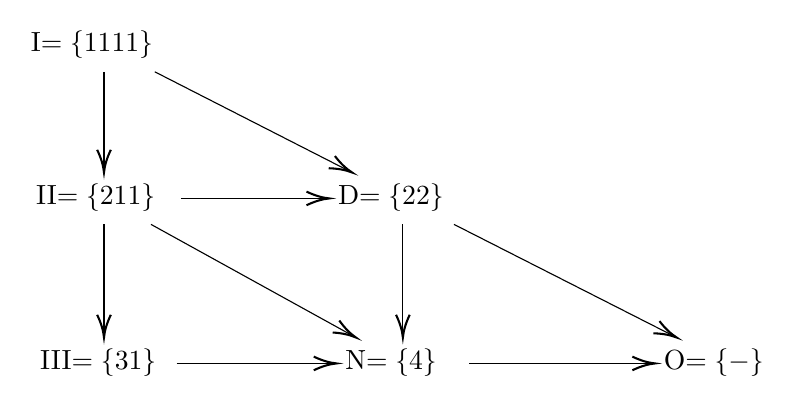
\begin{tikzpicture}[x=0.75pt,y=0.75pt,yscale=-1,xscale=1]
	%uncomment if require: \path (0,180); %set diagram left start at 0, and has height of 180
	
	
	
	% Text Node
	\draw (146,4) node [anchor=north west][inner sep=0.75pt]   [align=left] {I$=\{1111\}$};
	% Text Node
	\draw (148.5,77.5) node [anchor=north west][inner sep=0.75pt]   [align=left] {II$=\{211\}$};
	% Text Node
	\draw (294,77.5) node [anchor=north west][inner sep=0.75pt]   [align=left] {D$=\{22\}$};
	% Text Node
	\draw (150.5,157) node [anchor=north west][inner sep=0.75pt]   [align=left] {III$=\{31\}$};
	% Text Node
	\draw (297.5,157) node [anchor=north west][inner sep=0.75pt]   [align=left] {N$=\{4\}$};
	% Text Node
	\draw (451,157) node [anchor=north west][inner sep=0.75pt]   [align=left] {O$=\{-\}$};
	% Connection
	\draw    (182.5,25) -- (182.5,71.5) ;
	\draw [shift={(182.5,73.5)}, rotate = 270] [color={rgb, 255:red, 0; green, 0; blue, 0 }  ][line width=0.75]    (10.93,-3.29) .. controls (6.95,-1.4) and (3.31,-0.3) .. (0,0) .. controls (3.31,0.3) and (6.95,1.4) .. (10.93,3.29)   ;
	% Connection
	\draw    (206.99,25) -- (300.23,72.59) ;
	\draw [shift={(302.01,73.5)}, rotate = 207.04] [color={rgb, 255:red, 0; green, 0; blue, 0 }  ][line width=0.75]    (10.93,-3.29) .. controls (6.95,-1.4) and (3.31,-0.3) .. (0,0) .. controls (3.31,0.3) and (6.95,1.4) .. (10.93,3.29)   ;
	% Connection
	\draw    (219.5,86) -- (289,86) ;
	\draw [shift={(291,86)}, rotate = 180] [color={rgb, 255:red, 0; green, 0; blue, 0 }  ][line width=0.75]    (10.93,-3.29) .. controls (6.95,-1.4) and (3.31,-0.3) .. (0,0) .. controls (3.31,0.3) and (6.95,1.4) .. (10.93,3.29)   ;
	% Connection
	\draw    (182.5,98.5) -- (182.5,151) ;
	\draw [shift={(182.5,153)}, rotate = 270] [color={rgb, 255:red, 0; green, 0; blue, 0 }  ][line width=0.75]    (10.93,-3.29) .. controls (6.95,-1.4) and (3.31,-0.3) .. (0,0) .. controls (3.31,0.3) and (6.95,1.4) .. (10.93,3.29)   ;
	% Connection
	\draw    (217.5,165.5) -- (292.5,165.5) ;
	\draw [shift={(294.5,165.5)}, rotate = 180] [color={rgb, 255:red, 0; green, 0; blue, 0 }  ][line width=0.75]    (10.93,-3.29) .. controls (6.95,-1.4) and (3.31,-0.3) .. (0,0) .. controls (3.31,0.3) and (6.95,1.4) .. (10.93,3.29)   ;
	% Connection
	\draw    (205.14,98.5) -- (302.11,152.03) ;
	\draw [shift={(303.86,153)}, rotate = 208.9] [color={rgb, 255:red, 0; green, 0; blue, 0 }  ][line width=0.75]    (10.93,-3.29) .. controls (6.95,-1.4) and (3.31,-0.3) .. (0,0) .. controls (3.31,0.3) and (6.95,1.4) .. (10.93,3.29)   ;
	% Connection
	\draw    (326.5,98.5) -- (326.5,151) ;
	\draw [shift={(326.5,153)}, rotate = 270] [color={rgb, 255:red, 0; green, 0; blue, 0 }  ][line width=0.75]    (10.93,-3.29) .. controls (6.95,-1.4) and (3.31,-0.3) .. (0,0) .. controls (3.31,0.3) and (6.95,1.4) .. (10.93,3.29)   ;
	% Connection
	\draw    (351.11,98.5) -- (456.61,152.09) ;
	\draw [shift={(458.39,153)}, rotate = 206.93] [color={rgb, 255:red, 0; green, 0; blue, 0 }  ][line width=0.75]    (10.93,-3.29) .. controls (6.95,-1.4) and (3.31,-0.3) .. (0,0) .. controls (3.31,0.3) and (6.95,1.4) .. (10.93,3.29)   ;
	% Connection
	\draw    (358.5,165.5) -- (446,165.5) ;
	\draw [shift={(448,165.5)}, rotate = 180] [color={rgb, 255:red, 0; green, 0; blue, 0 }  ][line width=0.75]    (10.93,-3.29) .. controls (6.95,-1.4) and (3.31,-0.3) .. (0,0) .. controls (3.31,0.3) and (6.95,1.4) .. (10.93,3.29)   ;
	
\end{tikzpicture}
	\caption{根据主类光旋量方向的重合程度可以将外尔旋量分类成不同种类}
	\label{fig:Petrov}
\end{figure}

除此之外,根据外尔标量的定义,我们可以给出不同Petrov时空中,外尔标量为零的个数。如果我们选择$\xi ^{\boldsymbol{A}} =o^{\boldsymbol{A}}$,即$v^{\boldsymbol{a}} =l^{\boldsymbol{a}}$,那么
\begin{equation*}
	\upPsi _{\boldsymbol{ABCD}} o^{\boldsymbol{A}} o^{\boldsymbol{B}} o^{\boldsymbol{C}} o^{\boldsymbol{D}} =\upPsi _{0} ,
\end{equation*}
即如果时空为Petrov-I型,那么可以选择$\upPsi _{0} =0$。同样的,如果$l^{\boldsymbol{a}}$为Petrov-II型时空的主零方向,那么$\upPsi _{0} =\upPsi _{1} =0$。如果$l^{\boldsymbol{a}}$为Petrov-D型时空的第一个主零方向,且$n^{\boldsymbol{a}} =\iota ^{\boldsymbol{A}} \iota ^{\boldsymbol{A} '}$为第二个主零方向,那么除了$\upPsi _{0} =\upPsi _{1} =0$,我们还有$\upPsi _{4} =\upPsi _{3} =0$。同样的,III型和N型分别对应了$\upPsi _{0} =\upPsi _{1} =\upPsi _{2} =0$和$\upPsi _{0} =\upPsi _{1} =\upPsi _{2} =\upPsi _{3} =0$,而O型时空所有的外尔标量都为零,即共形平坦。


\subsection{哥德堡-萨赫定理}

现在我们考虑里奇张量为零,即黎曼张量与外尔张量重合的时空。这时我们有定理\parencite{chandrasekhar1998mathematical,goldberg2009republication}

\begin{them}[label={Goldberg-Sachs Theorem}]{哥德堡-萨赫定理(Goldberg-Sachs Theorem)}
	如果外尔张量是II型,且选择了$l^{\boldsymbol{a}}$作为主类光方向,即$\upPsi _{0} =\upPsi _{1} =0$,那么我们有
	\begin{equation*}
		\kappa =\sigma =0.
	\end{equation*}
	反之,如果$\kappa =\sigma =0$,那么
	\begin{equation*}
		\upPsi _{0} =\upPsi _{1} =0,
	\end{equation*}
	且外尔张量是II型。
\end{them}

\begin{proof}
	我们先来证明正命题。如果$\upPsi _{0} =\upPsi _{1} =0$,那么此时的比安基恒等式为
	\begin{equation*}
		\begin{cases}
			3\kappa \upPsi _{2} & =0\\
			D\upPsi _{2} & =-2\kappa \upPsi _{3} +3\rho \upPsi _{2}\\
			D\upPsi _{3} -\delta '\upPsi _{2} & =-\kappa \upPsi _{4} -2( \epsilon -\rho ) \upPsi _{3} +3\pi \upPsi _{2} ,
		\end{cases}
	\end{equation*}
	以及
	\begin{equation*}
		\begin{cases}
			3\sigma \upPsi _{2} & =0\\
			-\upDelta \upPsi _{2} & =2\sigma \upPsi _{3} -3\tau \upPsi _{2}\\
			D'\upPsi _{2} -\delta \upPsi _{3} & =-3\mu \upPsi _{2} -2( \tau -\beta ) \upPsi _{3} +\sigma \upPsi _{4} ,
		\end{cases}
	\end{equation*}
	由于时空不平坦,即$\upPsi _{2} ,\upPsi _{3} ,\upPsi _{4}$不全为零,那么$\kappa =\sigma =0$。
	
	
	
	现在来证明反论。由于标架有$6$个自由度,我们可以选择标架使得$\epsilon =0$,此时满足$\kappa =\sigma =0$,且包含这些量的里奇恒等式为
	\begin{equation}
		\begin{aligned}
			D\rho  & =\rho ^{2}\\
			\upPsi _{0} & =0\\
			D\tau  & =(\overline{\tau } +\pi )\rho +\upPsi _{1}
		\end{aligned}
		\label{eq:5.95}
	\end{equation}
	以及
	\begin{equation}
		\begin{aligned}
			D\beta  & =\overline{\rho } \beta +\upPsi _{1}\\
			\delta \rho  & =(\overline{\alpha } +\beta )\rho +(\rho -\overline{\rho } )\tau -\upPsi _{1} .
		\end{aligned}
		\label{eq:5.96}
	\end{equation}
	从\ref{eq:5.95}的第二个式子中我们给出$\upPsi _{0} =0$。此时,比安基恒等式为
	\begin{equation}
		\begin{aligned}
			D\upPsi _{1} & =4\rho \upPsi _{1}\\
			\delta \upPsi _{1} & =2(2\tau +\beta )\upPsi _{1} ,
		\end{aligned}
		\label{eq:5.97}
	\end{equation}
	以及$D,\delta $的对易子给出
	\begin{equation}
		D\delta -\delta D=(\overline{\pi } -\overline{\alpha } -\beta )D+\overline{\rho } \delta .
		\label{eq:5.98}
	\end{equation}
	现在,我们可以进一步选择规范使得$\tau =0$, 那么\ref{eq:5.97}给出
	\begin{equation*}
		\begin{cases}
			D\ln \upPsi _{1} & =4\rho ,\\
			\delta \ln \upPsi _{2} & =2\beta ,
		\end{cases}
	\end{equation*}
	故
	\begin{equation*}
		(D\delta -\delta D)\ln \upPsi _{1} =2D\beta -4\delta \rho .
	\end{equation*}
	现在,将上式的右侧带入\ref{eq:5.96}给出
	\begin{equation}
		(D\delta -\delta D)\ln \upPsi _{1} =2\overline{\rho } \beta -4(\overline{\alpha } +\beta )\rho +6\upPsi _{1} .
		\label{eq:5.99}
	\end{equation}
	然而,如果我们直接将对易子\ref{eq:5.98}应用在$\ln \upPsi _{1}$上,我们有
	\begin{equation}
		\begin{aligned}
			(D\delta -\delta D)\ln \upPsi _{1} & =(\overline{\pi } -\overline{\alpha } -\beta )D\ln \upPsi _{1} +\overline{\rho } \delta \ln \upPsi _{1}\\
			& =4(\overline{\pi } -\overline{\alpha } -\beta )\rho +2\beta \overline{\rho } .
		\end{aligned}
		\label{eq:5.100}
	\end{equation}
	为了保证\ref{eq:5.99}和\ref{eq:5.100}两侧相同,我们必须有
	\begin{equation*}
		\upPsi _{1} =\frac{2}{3}\overline{\pi } \rho ,
	\end{equation*}
	而\ref{eq:5.95}的第三式对于$\tau =0$有
	\begin{equation*}
		\upPsi _{1} =-\overline{\pi } \rho ,
	\end{equation*}
	这意味着我们必须有
	\begin{equation*}
		\upPsi _{1} =0.
	\end{equation*}
	至此正反两题证毕。
\end{proof}

哥德堡-萨赫定理的一个直接推论是,如果时空是Petrov-D型,那么当两个主类光方向$l^{\boldsymbol{a}} ,n^{\boldsymbol{a}}$重合时,即当且仅当
\begin{equation*}
	\upPsi _{0} =\upPsi _{1} =\upPsi _{3} =\upPsi _{4} =0
\end{equation*}
时,我们有
\begin{equation*}
	\kappa =\sigma =\nu =\lambda =0.
\end{equation*}
值得注意的是,广义相对论的黑洞解全部都是Petrov-D型的\parencite{chandrasekhar1998mathematical},因此我们总是能够令自旋系数$\kappa ,\sigma ,\lambda ,\nu $和除了$\upPsi _{2}$以外的外尔标量为零,这也是纽曼-彭罗斯形式对于它们特别有效的原因。

\chapter{物理的东西——时空中的场}


\section{电磁场及其导数}

在前面我们已经看到,引力场可以用一个对称旋量$\upPsi _{\boldsymbol{ABCD}}$刻画,同样的,电磁场也可以用一个对称旋量$\varphi _{\boldsymbol{AB}}$刻画。这个类比可以进一步扩展,每一个场都可以从其导数的对易子获得,在引力场的情况中就是普通的协变导数,而电磁场的情况是修改定义的协变导数。在平直时空中,我们只需要加上一项四矢势$A_{\boldsymbol{a}}$,即:
\begin{equation}
	\boldsymbol{\nabla }_{\boldsymbol{a}} \equiv \partial _{\boldsymbol{a}} -\mathrm{i} eA_{\boldsymbol{a}} ,
	\label{eq:6.1}
\end{equation}
这里$e$是电荷。现在,我们定义麦克斯韦场的场强$F_{\boldsymbol{ab}}$为$A_{\boldsymbol{a}}$的旋度:
\begin{equation*}
	\mathrm{i}\boldsymbol{\nabla }_{[\boldsymbol{a}}\boldsymbol{\nabla }_{\boldsymbol{b}]} \theta ^{\mathcal{A}} =e\theta ^{\mathcal{A}} \partial _{[\boldsymbol{a}} A_{\boldsymbol{b}]} =\frac{1}{2} e\theta ^{\mathcal{A}} F_{\boldsymbol{ab}} .
\end{equation*}
如果我们希望电磁场和引力场同时存在,这意味着我们需要将\ref{eq:6.1}中的$\partial _{\boldsymbol{a}}$变为普通的协变导数算符。 \ 



在经典理论中,我们的势能“$A_{\boldsymbol{a}}$”没有物理意义,同样的,$\upGamma {_{ab}}^{c}$对引力理论也没有直接的物理意义。因此,类似于我们在引力理论中所做的,我们不认为$\partial _{a}$是一个“本质的”量,对于带荷的理论同样如此,它是依赖于“规范”选取的。因此,我们希望构建一个更加“基本”的协变导数算符,使得用它构建出来的量都有“物理”或者“几何”意义。本节我们会用代数方法给出这样的协变导数的构造,并且这样的构造是适用于弯曲时空的版本的。


\section{带荷的场*}

我们之前曾经给出了流形上的$\mathbb{C}^{\infty }$旋量场——$\mathfrak{S}^{\mathcal{A}}$的定义,本章我们需要扩展其定义:对于每一个“荷”的值,都对应了一个模$\mathfrak{S}^{\mathcal{A}}$,而协变导数算符$\boldsymbol{\nabla }_{\boldsymbol{a}}$对于每一个版本都不同。我们引入带荷的模(charged modules):
\begin{equation*}
	\prescript{e}{}{}\mathfrak{S} ,\prescript{e}{}{}\mathfrak{S}^{\boldsymbol{A}} ,\cdots ,\prescript{e}{}{}\mathfrak{S}_{\boldsymbol{B} \cdots \boldsymbol{D} '\cdots }^{\boldsymbol{A} \cdots \boldsymbol{C} '\cdots } ,\cdots 
\end{equation*}
我们先前讨论的情况就是$e=0$的情况。原则上,$e$可以取任意复数,但是因为各种原因,我们将其取为整数,即$e$可以取值$0,\pm \varepsilon ,\cdots $。重点是$\prescript{e}{}{}\mathfrak{S}$中的元素,当$e\neq 0$的时候,在$\mathcal{M}$的每一点,它并不取一个具体的数值,而$\prescript{e}{}{}\mathfrak{S}[ P]$是一个抽象的一维可加的复向量空间,但是可能没有唯一的乘法单位元。同样,$\prescript{e}{}{}\mathfrak{S}[ P]$在两个不同的点处的取值也没有什么系统的联系。而正如一个矢量在选定基底后可以用数字描述其分量,$\prescript{e}{}{}\mathfrak{S}[ P]$中的元素在一个适当的\textbf{规范选取}后,也可以用某个数值标量描述。除了正常的构建模$\mathfrak{S}$的条件(包括各种操作,加乘缩并共轭),我们还有以下几个额外条件来构建$\prescript{e}{}{}\mathfrak{S}$。

\begin{post}[label={efraS needs}]{$\prescript{e}{}{}\mathfrak{S}$需要满足的}
	\begin{itemize}
		\item 两个带荷的旋量当且仅当它们的荷相同时才能相加。
		\item 无论两个选来那个的荷是怎样的,它们总是可以外乘。
		\item 指标缩并操作不影响荷的取值。
		\item 指标替换也不影响荷的取值。
		\item 复共轭操作会将荷变为相反数。
	\end{itemize}
\end{post}

现在我们考虑映射
\begin{equation*}
	\boldsymbol{\nabla }_{\boldsymbol{a}} :\prescript{e}{}{}\mathfrak{S}^{\mathcal{A}}\rightarrow \prescript{e}{}{}\mathfrak{S}_{a}^{\mathcal{A}} ,
\end{equation*}
注意这个映射是保证荷$e$不变的。如果我们知道了$\boldsymbol{\nabla }_{\boldsymbol{a}}$在$\prescript{\varepsilon }{}{}\mathfrak{S}$上的作用,通过考虑$\boldsymbol{\nabla }_{\boldsymbol{a}}$在无荷场上的作用,这样的$\boldsymbol{\nabla }_{\boldsymbol{a}}$是唯一的,即普通的协变导数。因为如果我们考察$\alpha \in \prescript{\varepsilon }{}{}\mathfrak{S} ,\psi ^{\mathcal{A}} \in \prescript{n\varepsilon }{}{}\mathfrak{S}^{\mathcal{A}}\prescript{}{}{}$,那么
\begin{equation*}
	\boldsymbol{\nabla }_{\boldsymbol{a}} \psi ^{\mathcal{A}} =\alpha ^{n}\boldsymbol{\nabla }_{\boldsymbol{a}} (\alpha ^{-n} \psi ^{\mathcal{A}} )+n\psi ^{\mathcal{A}} \alpha ^{-1}\boldsymbol{\nabla }_{\boldsymbol{a}} \alpha ,
\end{equation*}
由于$\alpha ^{-n} \psi ^{\mathcal{A}}$不带荷,而根据假设,我们也知道$\boldsymbol{\nabla }_{\boldsymbol{a}} \alpha $,因此我们可以将上式确定下来。这里需要注意,如果$\alpha \in \prescript{e}{}{}\mathfrak{S}$处处不为零,那么$\alpha ^{-1}$就表示了$\prescript{-e}{}{}\mathfrak{S}$中的唯一的元素。值得一提的是,全局存在带荷非零标量场的条件等价于在一个带磁荷的时空中没有“洞”。



由于$\epsilon _{\boldsymbol{AB}} ,\epsilon ^{\boldsymbol{AB}} ,\epsilon {_{\boldsymbol{A}}}^{\boldsymbol{B}}$被定义在无荷的模上,$\boldsymbol{\nabla }_{\boldsymbol{a}}$作用在它们身上的效果和普通的协变导数一致,因此给出零。



现在,我们来看看如何用$\boldsymbol{\nabla }_{\boldsymbol{a}}$的信息重构出$A_{\boldsymbol{a}}$和$\partial _{\boldsymbol{a}}$。类似于选择一个坐标基,我们也可以选择一个处处不为零的$\alpha \in \prescript{\varepsilon }{}{}\mathfrak{S}$,随后定义:
\begin{equation}
	A_{\boldsymbol{a}} \equiv \mathrm{i}( \varepsilon \alpha )^{-1}\boldsymbol{\nabla }_{\boldsymbol{a}} \alpha ,
	\label{eq:6.2}
\end{equation}
显然这个量是不带荷的。我们通过考虑在$\psi ^{\mathcal{A}}$(带有整数荷$e=n\varepsilon $)上的作用来定义对应的微分算符$\partial _{\boldsymbol{a}}$:
\begin{equation*}
	\partial _{\boldsymbol{a}} \psi ^{\mathcal{A}} \equiv \alpha ^{n}\boldsymbol{\nabla }_{\boldsymbol{a}} (\alpha ^{-n} \psi ^{\mathcal{A}} ),
\end{equation*}
那么
\begin{equation*}
	\boldsymbol{\nabla }_{\boldsymbol{a}} \psi ^{\mathcal{A}} =( \partial _{a} -\mathrm{i} eA_{\boldsymbol{a}}) \psi ^{\mathcal{A}} .
\end{equation*}
如果$e=0$,$\partial _{\boldsymbol{a}}$就是正常的\textbf{协变导数}(注意不是坐标导数)。在平直时空中,即使有电磁场的存在,我们有
\begin{equation*}
	\partial _{\boldsymbol{a}} \partial _{\boldsymbol{b}} =\partial _{\boldsymbol{b}} \partial _{\boldsymbol{a}} .
\end{equation*}
弯曲时空中,$\partial _{[\boldsymbol{a}} \partial _{\boldsymbol{b}]}$给出了曲率部分。



如果$\alpha $满足条件
\begin{equation*}
	\alpha \overline{\alpha } =1,\alpha \in \prescript{e}{}{}\mathfrak{S} ,
\end{equation*}
那么我们称$\alpha $为一个规范(gauge)。如果上式一开始不成立,那么根据$\alpha $处处不为零,我们可以做替换$\alpha \mapsto \alpha ( \alpha \overline{\alpha })^{-1/2}$来做到这件事。对于任何规范$\alpha $我们有
\begin{equation*}
	0=\boldsymbol{\nabla }_{\boldsymbol{a}}( \alpha \overline{\alpha }) =\alpha \boldsymbol{\nabla }_{\boldsymbol{a}}\overline{\alpha } +\overline{\alpha }\boldsymbol{\nabla }_{\boldsymbol{a}} \alpha \Rightarrow \overline{\alpha }^{-1}\boldsymbol{\nabla }\overline{\alpha } =-\alpha ^{-1}\boldsymbol{\nabla }_{\boldsymbol{a}} \alpha .
\end{equation*}
这意味着由\ref{eq:6.2}定义的$A_{\boldsymbol{a}}$是实的:
\begin{equation*}
	\overline{A}_{\boldsymbol{a}} =A_{\boldsymbol{a}} .
\end{equation*}
同样,对于任何规范,$\partial _{\boldsymbol{a}}$也是实的:
\begin{equation*}
	\overline{\partial _{\boldsymbol{a}} \psi ^{\mathcal{A}}} =\overline{\alpha ^{n}\boldsymbol{\nabla }_{\boldsymbol{a}} (\alpha ^{-n} \psi ^{\mathcal{A}} )} =\alpha ^{n}\boldsymbol{\nabla }_{\boldsymbol{a}} (\alpha ^{-n}\overline{\psi ^{\mathcal{A}}} )=\partial _{\boldsymbol{a}}\overline{\psi ^{\mathcal{A}}} .
\end{equation*}
规范$\alpha $可以将任何带荷的场映射到不带荷的场
\begin{equation*}
	\psi ^{\mathcal{A}} \mapsto \alpha ^{-n} \psi ^{\mathcal{A}} ,
\end{equation*}
那么在基底下,我们可以取数值分量,因为带荷的标量可能并没有一个正则的数值值。即如果我们要确定一个带荷场的分量,我们需要同时给出基底和规范的选取。如果一个规范$\alpha $被换成了另一个规范$\alpha '$,那么对应的不带荷的场也会经历一个规范变换:
\begin{equation*}
	\alpha ^{-n} \psi ^{\mathcal{A}} \mapsto \alpha ^{\prime -n} \psi ^{\mathcal{A}} =\mathrm{e}^{\mathrm{i} n\theta } (\alpha ^{-n} \psi ^{\mathcal{A}} ),
\end{equation*}
这里
\begin{equation*}
	\mathrm{e}^{\mathrm{i} \theta } =\alpha /a'.
\end{equation*}
对应的$A_{\boldsymbol{a}}$的变换规则为
\begin{equation}
	A_{\boldsymbol{a}} \mapsto A'_{\boldsymbol{a}} =\frac{\mathrm{i}}{\varepsilon \alpha '}\boldsymbol{\nabla }_{\boldsymbol{a}} \alpha '=\frac{\mathrm{i}}{\varepsilon \alpha }\mathrm{e}^{\mathrm{i} \theta }\boldsymbol{\nabla }_{\boldsymbol{a}} (\alpha \mathrm{e}^{-\mathrm{i} \theta } )=A_{\boldsymbol{a}} +\frac{1}{\varepsilon }\boldsymbol{\nabla }_{\boldsymbol{a}} \theta ,
	\label{eq:6.3}
\end{equation}
以及
\begin{equation*}
	\partial _{\boldsymbol{a}} \psi ^{\mathcal{A}} \mapsto (\partial _{\boldsymbol{a}} -\mathrm{i} e\boldsymbol{\nabla }_{\boldsymbol{a}} \theta )\psi ^{\mathcal{A}} .
\end{equation*}
这就是一般电磁理论中的规范变换。值得注意的是,在电磁学以及引力的情况,其规范变换都是“第二类”的,即不改变算符$\partial _{\boldsymbol{a}}$。电磁学的情况是显然的,因为$\alpha \mapsto \alpha '=\mathrm{e}^{-\mathrm{i} \theta } \alpha $,其中$\theta $是实的且是常数。在引力的情况中,我们的规范变换为$x^{a} \mapsto A{_{b}}^{a} x^{b} +B^{a}$,这里$A{_{b}}^{a}$和$B^{a}$都是实的常数矩阵且$\det A\neq 0$。如果我们令$A{_{b}}^{a}$是一个限制性洛伦兹变换,那么规范$x^{a}$的选取对应了一个将时空$\mathcal{M}$映射到闵氏空间的映射,其对称性被视为规范自由度。


\subsection{麦克斯韦场张量}

下面我们考虑对易子:
\begin{equation*}
	\upDelta _{\boldsymbol{ab}} =\boldsymbol{\nabla }_{\boldsymbol{a}}\boldsymbol{\nabla }_{\boldsymbol{b}} -\boldsymbol{\nabla }_{\boldsymbol{b}}\boldsymbol{\nabla }_{\boldsymbol{a}} =2\boldsymbol{\nabla }_{[\boldsymbol{a}}\boldsymbol{\nabla }_{\boldsymbol{b}]} ,
\end{equation*}
我们假设无挠,那么对于一个无荷的标量$\gamma \in \mathfrak{S}$,我们有:
\begin{equation*}
	\upDelta _{\boldsymbol{ab}} \gamma =0.
\end{equation*}
现在考虑$0\neq \alpha \in \prescript{\varepsilon }{}{}\mathfrak{S}$,那么对于$\psi \in \prescript{e}{}{}\mathfrak{S} ,e=n\varepsilon $,我们总有$\gamma \in \mathfrak{S}$,使得
\begin{equation*}
	\gamma \alpha ^{n} =\psi .
\end{equation*}
这意味着
\begin{equation*}
	\upDelta _{\boldsymbol{ab}} \psi =\gamma \upDelta _{\boldsymbol{ab}} \alpha ^{n} =n\gamma \alpha ^{n-1} \upDelta _{\boldsymbol{ab}} \alpha \Rightarrow n\psi \alpha ^{-1} \upDelta _{\boldsymbol{ab}} \alpha =\upDelta _{\boldsymbol{ab}} \psi .
\end{equation*}
如果我们令
\begin{equation}
	F_{\boldsymbol{ab}} \equiv \frac{\mathrm{i}}{\varepsilon \alpha } \upDelta _{\boldsymbol{ab}} \alpha \Rightarrow \mathrm{i} \upDelta _{\boldsymbol{ab}} \psi =eF_{\boldsymbol{ab}} \psi .
	\label{eq:6.4}
\end{equation}
可以看到这样定义的$F$是不依赖于规范$\alpha $的选择的。我们称这样的$F_{\boldsymbol{ab}}$为麦克斯韦或者电磁场张量。对于一个带荷的旋量$\psi ^{\mathcal{A}} \in \prescript{e}{}{}\mathfrak{S}^{\mathcal{A}}$,我们有:
\begin{equation*}
	\upDelta _{\boldsymbol{ab}} (\alpha ^{-n} \psi ^{\mathcal{A}} )=-n\alpha ^{-n-1} \psi ^{\mathcal{A}} \upDelta _{\boldsymbol{ab}} \alpha +\alpha ^{-n} \upDelta _{\boldsymbol{ab}} \psi ^{\mathcal{A}} ,
\end{equation*}
即
\begin{equation}
	\upDelta _{\boldsymbol{ab}} \psi ^{\mathcal{A}} =\alpha ^{n} \upDelta _{\boldsymbol{ab}} (\alpha ^{-n} \psi ^{\mathcal{A}} )-\mathrm{i} eF_{\boldsymbol{ab}} \psi ^{\mathcal{A}} ,
	\label{eq:6.5}
\end{equation}
由于$\alpha ^{-n} \psi ^{\mathcal{A}}$无荷,$\upDelta _{\boldsymbol{ab}} (\alpha ^{-n} \psi ^{\mathcal{A}} )$只是普通的协变导数算符,故
\begin{equation}
	\upDelta _{\boldsymbol{ab}} \psi ^{\mathcal{A}} =2\partial _{[\boldsymbol{a}} \partial _{\boldsymbol{b}]} \psi ^{\mathcal{A}} -\mathrm{i} eF_{\boldsymbol{ab}} \psi ^{\mathcal{A}} .
	\label{eq:6.6}
\end{equation}
由于$\partial _{\boldsymbol{a}}$是普通的协变导数算符,我们可以写出
\begin{equation*}
	\upDelta _{\boldsymbol{ab}} \psi _{\boldsymbol{c}} =-R{_{\boldsymbol{abc}}}^{\boldsymbol{d}} \psi _{\boldsymbol{d}} -\mathrm{i} eF_{\boldsymbol{ab}} \psi _{\boldsymbol{c}} .
\end{equation*}
现在我们考察$F_{\boldsymbol{ab}}$的性质。首先显然它是反对称的$F_{\boldsymbol{ab}} =-F_{\boldsymbol{ba}}$,同时由于$\boldsymbol{\nabla }_{\boldsymbol{a}}$不改变荷,根据\ref{eq:6.4},$F_{\boldsymbol{ab}}$是\textbf{无荷}的。如果对\ref{eq:6.4}取复共轭,我们有
\begin{equation*}
	\upDelta _{\boldsymbol{ab}}\overline{\psi } =\mathrm{i} eF_{\boldsymbol{ab}}\overline{\psi } ,
\end{equation*}
因为$\boldsymbol{\nabla }_{\boldsymbol{a}} =\overline{\boldsymbol{\nabla }}_{\boldsymbol{a}}$,这意味着$F_{\boldsymbol{ab}}$是实的。同样的,我们也有类似于比安基恒等式的结果:
\begin{equation*}
	\boldsymbol{\nabla }_{[\boldsymbol{a}}\boldsymbol{\nabla }_{\boldsymbol{b}}\boldsymbol{\nabla }_{\boldsymbol{c}]} \psi =\boldsymbol{\nabla }_{[\boldsymbol{a}}\boldsymbol{\nabla }_{[\boldsymbol{b}}\boldsymbol{\nabla }_{\boldsymbol{c}]]} \psi =-\frac{1}{2}\mathrm{i} e\boldsymbol{\nabla }_{[\boldsymbol{a}} (F_{\boldsymbol{bc}]} \psi )=-\frac{1}{2}\mathrm{i} e\psi \boldsymbol{\nabla }_{[\boldsymbol{a}} F_{\boldsymbol{bc}]} -\frac{1}{2}\mathrm{i} eF_{[\boldsymbol{bc}}\boldsymbol{\nabla }_{\boldsymbol{a}]} \psi ,
\end{equation*}
但同时根据
\begin{equation*}
	\boldsymbol{\nabla }_{[\boldsymbol{a}}\boldsymbol{\nabla }_{\boldsymbol{b}}\boldsymbol{\nabla }_{\boldsymbol{c}]} \psi =\boldsymbol{\nabla }_{[[\boldsymbol{a}}\boldsymbol{\nabla }_{\boldsymbol{b}]}\boldsymbol{\nabla }_{\boldsymbol{c}]} \psi =-\frac{1}{2} R{_{[\boldsymbol{abc}]}}^{\boldsymbol{d}}\boldsymbol{\nabla }_{\boldsymbol{d}} \psi -\frac{1}{2}\mathrm{i} eF_{[\boldsymbol{ab}}\boldsymbol{\nabla }_{\boldsymbol{c}]} \psi ,
\end{equation*}
对比两式,我们有
\begin{equation}
	\boldsymbol{\nabla }_{[\boldsymbol{a}} F_{\boldsymbol{bc}]} =0.
	\label{eq:6.7}
\end{equation}
如果我们选取一个规范$\alpha $,那么根据\ref{eq:6.2}:
\begin{equation*}
	\boldsymbol{\nabla }_{[\boldsymbol{a}} A_{\boldsymbol{b}]} \equiv \boldsymbol{\nabla }\mathrm{_{[\boldsymbol{a}}} [\mathrm{i} (\varepsilon \alpha )^{-1}\boldsymbol{\nabla }_{\boldsymbol{b}]} \alpha ]=-(\mathrm{i} /\varepsilon \alpha ^{2} )(\boldsymbol{\nabla }_{[\boldsymbol{a}} \alpha )(\boldsymbol{\nabla }_{\boldsymbol{b}]} \alpha )+(\mathrm{i} /\varepsilon \alpha )\boldsymbol{\nabla }_{[\boldsymbol{a}}\boldsymbol{\nabla }_{\boldsymbol{b}]} \alpha =\frac{1}{2} F_{\boldsymbol{ab}} ,
\end{equation*}
这意味着
\begin{equation}
	F_{\boldsymbol{ab}} =\boldsymbol{\nabla }_{\boldsymbol{a}} A_{\boldsymbol{b}} -\boldsymbol{\nabla }_{\boldsymbol{b}} A_{\boldsymbol{a}} .
	\label{eq:6.8}
\end{equation}
这就是我们在麦克斯韦理论中的通常的$F$的表达式。这意味着如果$F_{\boldsymbol{ab}} =0$,那么$A_{\boldsymbol{a}}$可以表示为一个梯度的形式$A_{\boldsymbol{a}} =\boldsymbol{\nabla }_{\boldsymbol{a}} \chi $,这里$\chi $是实的且不带荷。实际上,如果反过来,在局域也一定存在一个规范$\alpha $,其给出的势满足\ref{eq:6.8}。因为如果假设有两个不同的$A_{\boldsymbol{a}} ,A'_{\boldsymbol{a}}$,这意味着$\boldsymbol{\nabla }_{[\boldsymbol{a}} (A'_{\boldsymbol{b}]} -A_{\boldsymbol{b}]} )=0$,那么$A'_{\boldsymbol{a}} -A_{\boldsymbol{a}} =\varepsilon ^{-1}\boldsymbol{\nabla }_{\boldsymbol{a}} \theta $,由此根据\ref{eq:6.3},由$\alpha '$产生的势也总满足\ref{eq:6.8}。



众所周知比安基恒等式\ref{eq:6.7}给出了一半的麦克斯韦方程,如果我们定义流$J^{\boldsymbol{a}}$,那么另一半的麦克斯韦方程为
\begin{equation}
	\boldsymbol{\nabla }_{\boldsymbol{a}} F^{\boldsymbol{ab}} =4\pi J^{\boldsymbol{b}} .
	\label{eq:6.9}
\end{equation}
这个式子告诉我们$J^{\boldsymbol{a}}$是无荷的。


\subsection{电磁场旋量}

由于$F_{\boldsymbol{ab}}$是实的反对称张量,我们可以将其分解为
\begin{equation}
	F_{\boldsymbol{ab}} =\varphi _{\boldsymbol{AB}} \epsilon _{\boldsymbol{A} '\boldsymbol{B} '} +\epsilon _{\boldsymbol{AB}}\overline{\varphi }_{\boldsymbol{A} '\boldsymbol{B} '} ,
	\label{eq:6.10}
\end{equation}
这里$\varphi _{\boldsymbol{AB}}$被称为电磁旋量(electromagnetic spinor),其中
\begin{equation*}
	\varphi _{\boldsymbol{AB}} =\varphi _{(\boldsymbol{AB})} =\frac{1}{2} F{_{\boldsymbol{ABC} '}}^{\boldsymbol{C} '} .
\end{equation*}
我们也可以将$F_{\boldsymbol{ab}}$分成自对偶部分和反自对偶部分:
\begin{equation*}
	\prescript{-}{}{} F_{\boldsymbol{ab}} =\varphi _{\boldsymbol{AB}} \epsilon _{\boldsymbol{A} '\boldsymbol{B} '} ,\kern+0.4em \prescript{+}{}{} F_{\boldsymbol{ab}} =\epsilon _{\boldsymbol{AB}}\overline{\varphi }_{\boldsymbol{A} '\boldsymbol{B} '} .
\end{equation*}
从这里我们也可以看出,由于$F_{\boldsymbol{ab}}$的有效部分是两个旋量$\varphi _{\boldsymbol{AB}} ,\overline{\varphi }_{\boldsymbol{A} '\boldsymbol{B} '}$,前者有两个不带撇的指标,属于洛伦兹群的$( 1,0)$表示的表示空间,同时后者属于$( 0,1)$表示的表示空间,即电磁场$F_{\boldsymbol{ab}}$具有洛伦兹变换类型$( 1,0) \oplus ( 0,1)$。

除此之外,我们也可以根据\ref{eq:6.4},由$\upDelta _{\boldsymbol{ab}} =\epsilon _{\boldsymbol{A} '\boldsymbol{B} '} \Box _{\boldsymbol{AB}} +\epsilon _{\boldsymbol{AB}} \Box _{\boldsymbol{A} '\boldsymbol{B} '}$将$F$化为$\Box $的组合。例如考虑$\psi \in \prescript{e}{}{}\mathfrak{S}$。那么
\begin{equation*}
	\Box _{\boldsymbol{AB}} \psi =\frac{1}{2} \epsilon ^{\boldsymbol{A} '\boldsymbol{B} '} \upDelta _{\boldsymbol{ab}} \psi =-\frac{1}{2}\mathrm{i} e\epsilon ^{\boldsymbol{A} '\boldsymbol{B} '} F_{\boldsymbol{ab}} \psi =-\mathrm{i} e\varphi _{\boldsymbol{AB}} \psi ,
\end{equation*}
以及
\begin{equation*}
	\Box _{\boldsymbol{AB} '} \psi =-\mathrm{i} e\overline{\varphi }_{\boldsymbol{A} '\boldsymbol{B} '} \psi .
\end{equation*}
当$\psi ^{\mathcal{A}} \in \prescript{e}{}{}\mathfrak{S}^{\mathcal{A}}$,那么根据\ref{eq:6.5},我们知道
\begin{equation*}
	\Box _{\boldsymbol{AB}} \psi ^{\mathcal{A}} =\alpha ^{n} \Box _{\boldsymbol{AB}} (\alpha ^{-n} \psi ^{\mathcal{A}} )-\mathrm{i} e\varphi _{\boldsymbol{AB}} \psi ^{\mathcal{A}} ,
\end{equation*}
由于在无荷情况下$\Box _{\boldsymbol{AB}} \kappa ^{\boldsymbol{C}} =X{_{\boldsymbol{ABE}}}^{\boldsymbol{C}} \kappa ^{\boldsymbol{E}} ,\kern+0.4em \Box _{\boldsymbol{A} '\boldsymbol{B} '} \kappa ^{\boldsymbol{C}} =\upPhi {_{\boldsymbol{A} '\boldsymbol{B} '\boldsymbol{E}}}^{\boldsymbol{C}} \kappa ^{\boldsymbol{E}}$,我们知道
\begin{equation*}
	\begin{aligned}
		\Box _{\boldsymbol{AB}} \psi ^{\boldsymbol{D}} & =X{_{\boldsymbol{ABC}}}^{\boldsymbol{D}} \psi ^{\boldsymbol{C}} -\mathrm{i} e\varphi _{\boldsymbol{AB}} \psi ^{\boldsymbol{D}} ,\\
		\Box _{\boldsymbol{A'B} '} \psi ^{\boldsymbol{D}} & =\upPhi {_{\boldsymbol{A'B'C}}}^{\boldsymbol{D}} \psi ^{\boldsymbol{C}} -\mathrm{i} e\overline{\varphi }_{\boldsymbol{A'B} '} \psi ^{\boldsymbol{D}} .
	\end{aligned}
\end{equation*}
对比\ref{eq:6.8}和\ref{eq:6.10},我们知道
\begin{equation}
	\varphi _{\boldsymbol{AB}} =\boldsymbol{\nabla }_{\boldsymbol{A} '(\boldsymbol{A}} A{_{\boldsymbol{B})}}^{\boldsymbol{A} '} .
	\label{eq:6.11}
\end{equation}
(在平直时空中,)我们常常会对$A_{\boldsymbol{a}}$施加洛伦茨规范条件:
\begin{equation*}
	\boldsymbol{\nabla }^{\boldsymbol{a}} A_{\boldsymbol{a}} =0,
\end{equation*}
根据\ref{eq:6.2},这等价于
\begin{equation*}
	\alpha \boldsymbol{\nabla }^{\boldsymbol{a}}\boldsymbol{\nabla }_{\boldsymbol{a}} \alpha =(\boldsymbol{\nabla }^{\boldsymbol{a}} \alpha )(\boldsymbol{\nabla }_{\boldsymbol{a}} \alpha ),
\end{equation*}
在这个条件下,\ref{eq:6.11}可以化简为
\begin{equation*}
	\varphi _{\boldsymbol{AB}} =\boldsymbol{\nabla }_{\boldsymbol{A} '\boldsymbol{A}} A^{\boldsymbol{A} '}{}_{\boldsymbol{B}} .
\end{equation*}


现在,麦克斯韦方程组\ref{eq:6.9}可以被写成:
\begin{equation}
	\boldsymbol{\nabla }^{\boldsymbol{A} '\boldsymbol{B}} \varphi ^{\boldsymbol{A}}{}_{\boldsymbol{B}} +\boldsymbol{\nabla }^{\boldsymbol{AB} '}\overline{\varphi }^{\boldsymbol{A} '}{}_{\boldsymbol{B} '} =4\pi J^{\boldsymbol{AA} '} .
	\label{eq:6.12}
\end{equation}
同时,\ref{eq:6.7}也等价于$\boldsymbol{\nabla }_{\boldsymbol{a}}\prescript{*}{}{} F^{\boldsymbol{ab}} =0$,而$\prescript{*}{}{} F^{\boldsymbol{ab}} =-\mathrm{i} \varphi ^{\boldsymbol{AB}} \epsilon ^{\boldsymbol{A} '\boldsymbol{B} '} +\mathrm{i} \epsilon ^{\boldsymbol{AB}}\overline{\varphi }^{\boldsymbol{A} '\boldsymbol{B} '}$,从而我们知道
\begin{equation}
	\boldsymbol{\nabla }^{\boldsymbol{A} '\boldsymbol{B}} \varphi ^{\boldsymbol{A}}{}_{\boldsymbol{B}} =\boldsymbol{\nabla }^{\boldsymbol{AB} '}\overline{\varphi }^{\boldsymbol{A}}{}_{\boldsymbol{B}} ,
	\label{eq:6.13}
\end{equation}
现在两个麦克斯韦方程组\ref{eq:6.12},\ref{eq:6.13}可以被化为一个方程:
\begin{equation}
	\boldsymbol{\nabla }^{\boldsymbol{A} '\boldsymbol{B}} \varphi ^{\boldsymbol{A}}{}_{\boldsymbol{B}} =2\pi J^{\boldsymbol{AA} '} ,
	\label{eq:6.14}
\end{equation}
以及约束条件$J^{\boldsymbol{a}}$是实的:$J^{\boldsymbol{AA} '} =\overline{J}^{\boldsymbol{AA} '}$。



所谓的流守恒方程
\begin{equation*}
	\boldsymbol{\nabla }_{\boldsymbol{a}} J^{\boldsymbol{a}} =0
\end{equation*}
可以直接从方程\ref{eq:6.14}给出:
\begin{equation*}
	\begin{aligned}
		-2\pi \boldsymbol{\nabla }_{\boldsymbol{a}} J^{\boldsymbol{a}} =\boldsymbol{\nabla }_{\boldsymbol{AA} '}\boldsymbol{\nabla }^{\boldsymbol{A} '}{}_{\boldsymbol{B}} \varphi ^{\boldsymbol{AB}} =\Box _{\boldsymbol{AB}} \varphi ^{\boldsymbol{AB}} & =X{_{\boldsymbol{ABQ}}}^{\boldsymbol{A}} \varphi ^{\boldsymbol{QB}} +X{_{\boldsymbol{ABQ}}}^{\boldsymbol{B}} \varphi ^{\boldsymbol{AQ}}\\
		& =3\upLambda (\epsilon _{\boldsymbol{BQ}} \varphi ^{\boldsymbol{QB}} +\epsilon _{\boldsymbol{AQ}} \varphi ^{\boldsymbol{AQ}} )=0.
	\end{aligned}
\end{equation*}
如果我们将\ref{eq:6.11}带入\ref{eq:6.14},我们知道
\begin{equation*}
	\boldsymbol{\nabla }^{\boldsymbol{A} '}{}_{\boldsymbol{B}}\boldsymbol{\nabla }^{\boldsymbol{C} '(\boldsymbol{A}} A^{\boldsymbol{B})}{}_{\boldsymbol{C} '} =2\pi J^{\boldsymbol{AA} '} ,
\end{equation*}
如果取洛伦茨规范条件给出$\varphi _{\boldsymbol{AB}} =\boldsymbol{\nabla }_{\boldsymbol{A} '\boldsymbol{A}} \upPhi ^{\boldsymbol{A} '}{}_{\boldsymbol{B}}$,这意味着$\boldsymbol{AB}$指标天然对称,因此我们可以写:
\begin{equation*}
	\begin{aligned}
		2\pi J^{\boldsymbol{AA} '} & =\boldsymbol{\nabla }^{\boldsymbol{A} '}{}_{\boldsymbol{B}}\boldsymbol{\nabla }^{\boldsymbol{C} '\boldsymbol{B}} A^{\boldsymbol{A}}{}_{\boldsymbol{C} '}\\
		& =\boldsymbol{\nabla }^{(\boldsymbol{A} '}{}_{\boldsymbol{B}}\boldsymbol{\nabla }^{\boldsymbol{C} ')\boldsymbol{B}} A^{\boldsymbol{A}}{}_{\boldsymbol{C} '} +\boldsymbol{\nabla }^{[\boldsymbol{A} '}{}_{\boldsymbol{B}}\boldsymbol{\nabla }^{\boldsymbol{C} ']\boldsymbol{B}} A^{\boldsymbol{A}}{}_{\boldsymbol{C} '}\\
		& =\Box ^{\boldsymbol{A} '\boldsymbol{C} '} A^{\boldsymbol{A}}{}_{\boldsymbol{C} '} +\frac{1}{2} \epsilon ^{\boldsymbol{A} '\boldsymbol{C} '}\boldsymbol{\nabla }_{\boldsymbol{BB} '}\boldsymbol{\nabla }^{\boldsymbol{BB} '} A^{\boldsymbol{A}}{}_{\boldsymbol{C} '}\\
		& =-\upPhi ^{\boldsymbol{AA} '}{}_{\boldsymbol{CC} '} A^{\boldsymbol{CC} '} +3\upLambda A^{\boldsymbol{AA} '} +\frac{1}{2}\boldsymbol{\nabla }{_{\boldsymbol{b}}}^{\boldsymbol{b}} A^{\boldsymbol{a}} ,
	\end{aligned}
\end{equation*}
这意味着
\begin{equation*}
	4\pi J^{\boldsymbol{a}} =\boldsymbol{\nabla }_{\boldsymbol{b}}\boldsymbol{\nabla }^{\boldsymbol{a}} A^{\boldsymbol{a}} +R^{\boldsymbol{a}}{}_{\boldsymbol{c}} A^{\boldsymbol{c}} .
\end{equation*}


此外,如果$J^{\boldsymbol{a}} =0$,那么
\begin{equation*}
	\boldsymbol{\nabla }^{\boldsymbol{AA} '} \varphi _{\boldsymbol{AB}} =0,
\end{equation*}
这是无源麦克斯韦方程组$\boldsymbol{\nabla }_{[\boldsymbol{a}} F_{\boldsymbol{bc}]} =0,\boldsymbol{\nabla }_{\boldsymbol{a}} F^{\boldsymbol{ab}} =0$的旋量形式,这与自旋$2$的无质量粒子的场方程形式一致。


\subsection{与三矢量的关系*}

如果我们将$F_{\boldsymbol{ab}}$在闵氏标架$t^{\boldsymbol{a}} ,x^{\boldsymbol{a}} ,y^{\boldsymbol{a}} ,z^{\boldsymbol{a}}$下展开,那么其分量与三维的矢量场$\boldsymbol{E} ,\boldsymbol{B}$的关系为:
\begin{equation}
	F_{ab} =\begin{pmatrix}
		0 & E_{1} & E_{2} & E_{3}\\
		-E_{1} & 0 & -B_{3} & B_{2}\\
		-E_{2} & B_{3} & 0 & -B_{1}\\
		-E_{3} & -B_{2} & B_{1} & 0
	\end{pmatrix} .
	\label{eq:6.15}
\end{equation}
那么根据张量分量与旋量分量之间的转化关系,取范德瓦尔登符号$g{_{\boldsymbol{AA} '}}^{\boldsymbol{a}}$为标准的泡利矩阵,我们知道
\begin{equation}
	\begin{aligned}
		\varphi _{00} & =\frac{1}{2} (F_{31} +F_{01} -\mathrm{i} F_{32} -\mathrm{i} F_{02} )=\frac{1}{2}( C_{1} -\mathrm{i} C_{2})\\
		\varphi _{01} & =\frac{1}{2} (-F_{03} -\mathrm{i} F_{12} )=-\frac{1}{2} C_{3}\\
		\varphi _{11} & =\frac{1}{2}( F_{31} -F_{01} +\mathrm{i} F_{32} -\mathrm{i} F_{02}) =-\frac{1}{2}( C_{1} +\mathrm{i} C_{2}) ,
	\end{aligned}
	\label{eq:6.16}
\end{equation}
其中
\begin{equation}
	\boldsymbol{C} =\boldsymbol{E} -\mathrm{i}\boldsymbol{B} .
	\label{eq:6.17}
\end{equation}
反过来,如果我们记
\begin{equation}
	\begin{aligned}
		\varphi _{0} & =\varphi _{00} & \varphi _{1} & =\varphi _{01} & \varphi _{2} & =\varphi _{11}\\
		\overline{\varphi }_{0} & =\varphi _{0'0'} & \overline{\varphi }_{1} & =\varphi _{0'1'} & \overline{\varphi }_{2} & =\varphi _{1'1'} ,
	\end{aligned}
	\label{eq:6.18}
\end{equation}
那么
\begin{equation*}
	\begin{array}{ l }
		F_{ab} = \\
		{\footnotesize \frac{1}{2} \times\begin{pmatrix}
			0 & ( \varphi _{0} -\varphi _{2} +\overline{\varphi }_{0} -\overline{\varphi }_{2}) & (\mathrm{i} \varphi _{0} +\mathrm{i} \varphi _{2} -\mathrm{i}\overline{\varphi }_{0} -\mathrm{i}\overline{\varphi }_{2}) & ( -2\varphi _{1} -2\overline{\varphi }_{1})\\
			( -\varphi _{0} +\varphi _{2} -\overline{\varphi }_{0} +\overline{\varphi }_{2}) & 0 & ( 2\mathrm{i} \varphi _{1} -2\mathrm{i}\overline{\varphi }_{1}) & ( -\varphi _{0} -\varphi _{2} -\overline{\varphi }_{0} -\overline{\varphi }_{2})\\
			( -\mathrm{i} \varphi _{0} -\mathrm{i} \varphi _{2} +\mathrm{i}\overline{\varphi }_{0} +\mathrm{i}\overline{\varphi }_{1}) & ( -2\mathrm{i} \varphi _{1} +2\mathrm{i}\overline{\varphi }_{1}) & 0 & (\mathrm{i} \varphi _{2} -\mathrm{i} \varphi _{0} -\mathrm{i}\overline{\varphi }_{2} +\mathrm{i}\overline{\varphi }_{0})\\
			( 2\varphi _{1} +2\overline{\varphi }_{1}) & ( \varphi _{0} +\varphi _{2} +\overline{\varphi }_{0} +\overline{\varphi }_{2}) & ( -\mathrm{i} \varphi _{2} +\mathrm{i} \varphi _{0} +\mathrm{i}\overline{\varphi }_{2} -\mathrm{i}\overline{\varphi }_{0}) & 0
		\end{pmatrix}} .
	\end{array}
\end{equation*}
如果$F_{\boldsymbol{ab}}$是复的场并且满足无源麦克斯韦场方程,那么它是单光子的“波函数”。这种情况下,我们写
\begin{equation*}
	F_{\boldsymbol{ab}} =\varphi _{\boldsymbol{AB}} \epsilon _{\boldsymbol{A} '\boldsymbol{B} '} +\epsilon _{\boldsymbol{AB}}\tilde{\varphi }_{\boldsymbol{A'B} '} ,
\end{equation*}
这里
\begin{equation*}
	\varphi _{\boldsymbol{AB}} =\frac{1}{2} F{_{\boldsymbol{ABC} '}}^{\boldsymbol{C} '} ,\kern+0.4em \tilde{\varphi }_{\boldsymbol{A} '\boldsymbol{B} '} =\frac{1}{2} F{_{\boldsymbol{C}}}^{\boldsymbol{C}}{}_{\boldsymbol{A} '\boldsymbol{B} '} ,
\end{equation*}
这里$\varphi _{\boldsymbol{AB}} ,\tilde{\varphi }_{\boldsymbol{A'B} '}$是两个无关的旋量场。此时\ref{eq:6.18}定义的关于$\varphi ,\tilde{\varphi }$的矩阵$F_{\boldsymbol{ab}}$仍然成立,只是需要将$\overline{\varphi }$替换为$\tilde{\varphi }$,\ref{eq:6.16}不变,对应的$\tilde{\varphi }$的定义式需要将\ref{eq:6.16}和\ref{eq:6.17}中的$\mathrm{i}$替换为$-\mathrm{i}$。



式\ref{eq:6.15}的对偶为
\begin{equation*}
	\prescript{*}{}{} F_{ab} =\begin{pmatrix}
		0 & -B_{1} & -B_{2} & -B_{3}\\
		B_{1} & 0 & -E_{3} & E_{2}\\
		B_{2} & E_{3} & 0 & -E_{1}\\
		B_{3} & -E_{2} & E_{1} & 0
	\end{pmatrix} ,
\end{equation*}
我们可以利用它定义两个重要的量:
\begin{equation*}
	\begin{aligned}
		P & =\frac{1}{2} F_{\boldsymbol{ab}} F^{\boldsymbol{ab}} =-\frac{1}{2}\prescript{*}{}{} F_{\boldsymbol{ab}}\prescript{*}{}{} F^{\boldsymbol{ab}} =\boldsymbol{B}^{2} -\boldsymbol{E}^{2} ,\\
		Q & =\frac{1}{2} F_{\boldsymbol{ab}}\prescript{*}{}{} F^{\boldsymbol{ab}} =2\boldsymbol{E} \cdot \boldsymbol{B} .
	\end{aligned}
\end{equation*}
以及:
\begin{equation*}
	K\equiv \varphi _{\boldsymbol{AB}} \varphi ^{\boldsymbol{AB}} =\frac{1}{2}\prescript{-}{}{} F_{\boldsymbol{ab}}\prescript{-}{}{} F^{\boldsymbol{ab}} =\frac{1}{2} F_{\boldsymbol{ab}}\prescript{-}{}{} F^{\boldsymbol{ab}} =P+\mathrm{i} Q.
\end{equation*}
如果$F_{\boldsymbol{ab}}$是实场,那么$P,Q$也是实的,那么他们可以分别作为$K$的实部和虚部。如果$F_{\boldsymbol{ab}}$是复的,那么我们定义
\begin{equation*}
	\tilde{K} \equiv \tilde{\varphi }_{\boldsymbol{A} '\boldsymbol{B} '}\tilde{\varphi }^{\boldsymbol{A} '\boldsymbol{B} '} =\frac{1}{2} F_{\boldsymbol{ab}}\prescript{+}{}{} F^{\boldsymbol{ab}} =P-\mathrm{i} Q,
\end{equation*}
那么我们有:
\begin{equation*}
	P=( K+\tilde{K}) /2,\kern+0.4em Q=( K-\tilde{K}) /2\mathrm{i} .
\end{equation*}
如果$P=Q=0$,那么场是类光的,即$\varphi _{\boldsymbol{AB}}$的两个主类光方向重合。如果$Q=0$但$P\neq 0$,且在实场的情况下,场要么是纯电场要么是纯磁场,前者$P< 0$,后者$P >0$、实际上,我们能找到(无穷多个)洛伦兹变换在电场和磁场之间变换。同时,$Q=0$也是$F_{\boldsymbol{ab}}$是单的条件,即一个反对称张量可以分解为
\begin{equation*}
	F_{\boldsymbol{ab} \cdots \boldsymbol{r}} =a_{[\boldsymbol{a}} b_{\boldsymbol{b}} \cdots r_{\boldsymbol{r}]} .
\end{equation*}

\section{爱因斯坦-麦克斯韦方程的旋量形式*}

现在我们考虑这样的理论:爱因斯坦场方程的唯一的源是电磁场的能动张量。



首先我们需要找出电磁场的能动张量的选来那个形式。考虑一个实对称张量$T_{\boldsymbol{ab}}$当电磁场无源时满足
\begin{equation}
	\boldsymbol{\nabla }^{\boldsymbol{a}} T_{\boldsymbol{ab}} =0
	\label{eq:6.19}
\end{equation}
且是电磁场$F_{\boldsymbol{ab}}$的二次型。显然,有一个形式的电磁场张量都满足这些条件:
\begin{equation*}
	T_{\boldsymbol{ab}} =k\varphi _{\boldsymbol{AB}}\overline{\varphi }_{\boldsymbol{A} '\boldsymbol{B} '} ,k\in \mathbb{R}^{+} .
\end{equation*}
这个形式的张量满足\ref{eq:6.19}因为无源$\boldsymbol{\nabla }^{\boldsymbol{AA} '} \varphi _{\boldsymbol{AB}} =0$。这和引力场的贝尔-罗宾逊张量的形式相同。



标准的电磁场能动张量的形式为
\begin{equation}
	\begin{aligned}
		T_{\boldsymbol{ab}} & =\frac{1}{4\pi }\left(\frac{1}{4} g_{\boldsymbol{ab}} F_{\boldsymbol{cd}} F^{\boldsymbol{cd}} -F_{\boldsymbol{ac}} F{_{\boldsymbol{b}}}^{\boldsymbol{c}}\right)\\
		& =-\frac{1}{8\pi } (F_{\boldsymbol{ab}} F{_{\boldsymbol{b}}}^{\boldsymbol{c}} +\prescript{*}{}{} F_{\boldsymbol{ac}}\prescript{*}{}{} F{_{\boldsymbol{b}}}^{\boldsymbol{c}} ).
	\end{aligned}
	\label{eq:6.20}
\end{equation}
带入$F$的旋量形式可以给出:
\begin{equation}
	T_{\boldsymbol{ab}} =\frac{1}{2\pi } \varphi _{\boldsymbol{AB}}\overline{\varphi }_{\boldsymbol{A} '\boldsymbol{B} '} .
	\label{eq:6.21}
\end{equation}
在电磁场的对偶性旋转$\varphi _{\boldsymbol{AB}} \mapsto \mathrm{e}^{-\mathrm{i} \theta } \varphi _{\boldsymbol{AB}}$下不变。除此之外,$T$也是无迹的:
\begin{equation*}
	T{_{\boldsymbol{a}}}^{\boldsymbol{a}} =0.
\end{equation*}
这些性质与引力场的贝尔-罗宾逊张量一致。现在我们将\ref{eq:6.21}带入引力场方程
\begin{equation*}
	\upPhi _{\boldsymbol{ab}} =4\pi \gamma \left( T_{\boldsymbol{ab}} -\frac{1}{4} T^{\boldsymbol{q}}{}_{\boldsymbol{q}} g_{\boldsymbol{ab}}\right) ,\kern+0.4em \upLambda =\frac{1}{3} \pi \gamma T^{\boldsymbol{q}}{}_{\boldsymbol{q}} +\frac{1}{6} \lambda ,
\end{equation*}
由于无迹,上式可以被化为
\begin{equation*}
	\upPhi _{\boldsymbol{ABA} '\boldsymbol{B}} =2\gamma \varphi _{\boldsymbol{AB}}\overline{\varphi }_{\boldsymbol{A} '\boldsymbol{B} '} ,\kern+0.4em \upLambda =\frac{1}{6} \lambda .
\end{equation*}
这两个方程与无源麦克斯韦场方程$\boldsymbol{\nabla }^{\boldsymbol{AA} '} \varphi _{\boldsymbol{AB}} =0$一起构成了爱因斯坦-麦克斯韦方程的旋量形式。通常我们也取$\lambda =0$。除此之外,如果我们将$T$的旋量形式带入之前得到的非真空场方程的形式$\boldsymbol{\nabla }^{\boldsymbol{A}}{}_{\boldsymbol{B} '} \upPsi _{\boldsymbol{ABCD}} =4\pi \gamma \boldsymbol{\nabla }^{\boldsymbol{A} '}{}_{(\boldsymbol{B}} T_{\boldsymbol{CD})\boldsymbol{A} '\boldsymbol{B} '}$:
\begin{equation*}
	\boldsymbol{\nabla }^{\boldsymbol{A}}{}_{\boldsymbol{B} '} \upPsi _{\boldsymbol{ABCD}} =2\gamma \boldsymbol{\nabla }^{\boldsymbol{A} '}{}_{(\boldsymbol{B}} (\varphi _{\boldsymbol{CD})}\overline{\varphi }_{\boldsymbol{A} '\boldsymbol{B} '} )=2\gamma (\overline{\varphi }_{\boldsymbol{A} '\boldsymbol{B} '}\boldsymbol{\nabla }^{\boldsymbol{A} '}{}_{(\boldsymbol{B}} \varphi _{\boldsymbol{CD})} +\varphi _{(\boldsymbol{CD}}\boldsymbol{\nabla }^{\boldsymbol{A} '}{}_{\boldsymbol{B})}\overline{\varphi }_{\boldsymbol{A} '\boldsymbol{B} '} ).
\end{equation*}
其中第二项因为场方程消失,而第一项的$\boldsymbol{BCD}$指标本身就是对称的,我们有:
\begin{equation*}
	\boldsymbol{\nabla }^{\boldsymbol{A}}{}_{\boldsymbol{B} '} \upPsi _{\boldsymbol{ABCD}} =2\gamma \overline{\varphi }_{\boldsymbol{A} '\boldsymbol{B} '}\boldsymbol{\nabla }^{\boldsymbol{A} '}{}_{(\boldsymbol{B}} \varphi _{\boldsymbol{CD})} .
\end{equation*}
这样,原先关于贝尔-罗宾逊张量的定义$T_{\boldsymbol{abcd}} =\upPsi _{\boldsymbol{ABCD}}\overline{\upPsi }_{\boldsymbol{A} '\boldsymbol{B} '\boldsymbol{C} '\boldsymbol{D} '}$的散度就不为零。我们可以修改其定义让其拥有零散度,但是修改后的张量不是全对称的:
\begin{equation*}
	\begin{aligned}
		T_{\boldsymbol{abcd}} = & \upPsi _{\boldsymbol{ABCD}}\overline{\upPsi }_{\boldsymbol{A} '\boldsymbol{B} '\boldsymbol{C} '\boldsymbol{D} '} -2\gamma \boldsymbol{\nabla }_{\boldsymbol{CD} '} \varphi _{\boldsymbol{AB}}\boldsymbol{\nabla }_{\boldsymbol{DC} '}\overline{\varphi }_{\boldsymbol{A} '\boldsymbol{B} '}\\
		& +6\gamma \boldsymbol{\nabla }_{\boldsymbol{D}(\boldsymbol{A} '|} \varphi _{(\boldsymbol{AB}}\boldsymbol{\nabla }_{\boldsymbol{C})\boldsymbol{D} '}\overline{\varphi }_{|\boldsymbol{B} '\boldsymbol{C} ')} -\lambda \varphi _{(\boldsymbol{AB}} \epsilon _{\boldsymbol{C})\boldsymbol{D}}\overline{\varphi }_{(\boldsymbol{A} '\boldsymbol{B} '} \epsilon _{\boldsymbol{C} ')\boldsymbol{D} '} .
	\end{aligned}
\end{equation*}
这样的张量的性质为:
\begin{equation*}
	T_{\boldsymbol{abcd}} =T_{(\boldsymbol{abc})\boldsymbol{d}} ,\kern+0.4em T^{\boldsymbol{a}}{}_{\boldsymbol{acd}} =0,\kern+0.4em \boldsymbol{\nabla }^{\boldsymbol{d}} T_{\boldsymbol{abcd}} =0.
\end{equation*}
\subsection{麦克斯韦能动张量的正定性*}

本节我们阐述$T_{\boldsymbol{ab}}$是正定的。



考虑任意两个旋量$\mu ^{\boldsymbol{A}} ,\nu ^{\boldsymbol{A}}$以及它们对应的类光方向$M^{\boldsymbol{a}} =\mu ^{\boldsymbol{A}}\overline{\mu }^{\boldsymbol{A} '} ,N^{\boldsymbol{a}} =\nu ^{\boldsymbol{A}}\overline{\nu }^{\boldsymbol{A} '}$,我们有:
\begin{equation*}
	T_{\boldsymbol{ab}} M^{\boldsymbol{a}} N^{\boldsymbol{b}} =\frac{1}{2\pi }\left| \varphi _{\boldsymbol{AB}} \mu ^{\boldsymbol{A}} \nu ^{\boldsymbol{B}}\right| ^{2} \geq 0,
\end{equation*}
这个不等式对于任意两个指向未来的类光矢量都成立。由于任何一个指向未来的因果矢量(类光和类时矢量)都是某些指向未来类光矢量的线性组合,因此我们有结论:

\begin{them}[label={them:dominant energy condition}]{主能量条件}
	对于任何一对指向未来的因果矢量$U^{\boldsymbol{a}} ,V^{\boldsymbol{a}}$都有
	\begin{equation*}
		T_{\boldsymbol{ab}} U^{\boldsymbol{a}} V^{\boldsymbol{a}} \geq 0.
	\end{equation*}
\end{them}

这个定理也可以被修改为:
\begin{them}[label={them:modified dominant energy condition}]{}
	对于任何一指向未来的因果矢量$V^{\boldsymbol{a}}$都有
	\begin{equation*}
		V^{\boldsymbol{a}} T{_{\boldsymbol{a}}}^{\boldsymbol{b}} T_{\boldsymbol{bc}} V^{\boldsymbol{c}} \geq 0,\kern+0.4em V^{\boldsymbol{a}} T_{\boldsymbol{ab}} V^{\boldsymbol{b}} \geq 0.
	\end{equation*}
\end{them}

我们常常称\ref{them:dominant energy condition}或\ref{them:modified dominant energy condition}为\textbf{主能量条件}(dominant energy condition)。因为如果$V^{\boldsymbol{a}}$为一个观者的$4$-速度,那么$T^{\boldsymbol{a}}{}_{\boldsymbol{b}} V^{\boldsymbol{b}}$为其坡印廷矢量,那么\ref{them:dominant energy condition}意味着能量流的速度(通过坡印廷矢量描述)不会超过光速。

如果我们把上述能量条件适当减弱:
\begin{equation*}
	T_{\boldsymbol{ab}} V^{\boldsymbol{a}} V^{\boldsymbol{b}} \geq 0,
\end{equation*}
就得到了弱能量条件,即观者观测到的能量密度$T_{00}$必须是其$4$-速度$V^{\boldsymbol{a}}$(作为其标架的基底$g{_{0}}^{\boldsymbol{a}}$)的非负定函数。极限情况下
\begin{equation*}
	T_{\boldsymbol{ab}} V^{\boldsymbol{a}} V^{\boldsymbol{b}} =0,
\end{equation*}
如果$V^{\boldsymbol{a}}$是类光矢量$N^{\boldsymbol{a}} =\nu ^{\boldsymbol{A}}\overline{\nu }^{\boldsymbol{A} '}$,那么$T_{\boldsymbol{ab}} N^{\boldsymbol{a}} N^{\boldsymbol{b}}$为零当且仅当
\begin{equation*}
	\varphi _{\boldsymbol{AB}} \nu ^{\boldsymbol{A}} \nu ^{\boldsymbol{B}} =0,
\end{equation*}
而这对应着$\nu ^{\boldsymbol{A}}$的旗杆指向$\varphi _{\boldsymbol{AB}}$的两个主类光方向其中之一。实际上我们可以给出:

\begin{them}[label={them:6.3}]{}
	如果$V^{\boldsymbol{a}}$是$\varphi _{\boldsymbol{AB}}$的主类光矢量,那么这等价于
	\begin{equation*}
		T_{\boldsymbol{ab}} V^{\boldsymbol{a}} V^{\boldsymbol{b}} =0,V^{\boldsymbol{a}} V_{\boldsymbol{a}} \geq 0,V^{\boldsymbol{a}} \neq 0.
	\end{equation*}
\end{them}
同样的结果对引力场的贝尔-罗宾逊张量也成立:
\begin{them}[label={them:6.4}]{}
	对于所有的指向未来的因果矢量$S^{\boldsymbol{a}} ,U^{\boldsymbol{a}} ,V^{\boldsymbol{a}} ,W^{\boldsymbol{a}}$,我们都有:
	\begin{equation*}
		T_{\boldsymbol{abcd}} S^{\boldsymbol{a}} U^{\boldsymbol{b}} V^{\boldsymbol{c}} W^{\boldsymbol{d}} \geq 0.
	\end{equation*}
	除此之外,如果$V^{\boldsymbol{a}}$是$\upPsi _{\boldsymbol{ABCD}}$的主类光矢量,那么这等价于
	\begin{equation*}
		T_{\boldsymbol{abcd}} V^{\boldsymbol{a}} V^{\boldsymbol{b}} V^{\boldsymbol{c}} V^{\boldsymbol{d}} =0,V^{\boldsymbol{a}} V_{\boldsymbol{a}} \geq 0,V^{\boldsymbol{a}} \neq 0.
	\end{equation*}
\end{them}
注意到贝尔-罗宾逊张量满足
\begin{equation*}
	T\boldsymbol{_{ABCDA'B'C'D'}} T\boldsymbol{_{EFGHE'F'G'H'}} =T\boldsymbol{_{ABCDE'F'G'H'}} T\boldsymbol{_{EFGHA'B'C'D'}} ,
\end{equation*}
而这在电磁学中的版本为
\begin{equation*}
	T_{\boldsymbol{ABA} '\boldsymbol{B} '} T_{\boldsymbol{CDC} '\boldsymbol{D} '} =T_{\boldsymbol{ABC} '\boldsymbol{D} '} T_{\boldsymbol{CDA} '\boldsymbol{B} '} ,
\end{equation*}
如果将其化为张量形式,我们有:
\begin{equation*}
	T_{\boldsymbol{ac}} T{_{\boldsymbol{b}}}^{\boldsymbol{c}} =\frac{1}{4} (T_{\boldsymbol{cd}} T^{\boldsymbol{cd}} )g_{\boldsymbol{ab}} .
\end{equation*}

\subsection{拉尼奇条件*}

我们已经看到麦克斯韦理论的能动张量有如下性质:
\begin{itemize}
	\item $T{_{\boldsymbol{a}}}^{\boldsymbol{a}} =0$
	\item $T_{\boldsymbol{ab}} T{_{\boldsymbol{c}}}^{\boldsymbol{d}} \propto g_{\boldsymbol{ac}}$
	\item 对于每一对指向未来的因果矢量$U^{\boldsymbol{a}} ,V^{\boldsymbol{a}}$都有$T_{\boldsymbol{ab}} U^{\boldsymbol{a}} V^{\boldsymbol{b}} \geq 0$
\end{itemize}

但是反过来,我们给出结论:对于在每一点都满足上面三个条件的实对称张量$T_{\boldsymbol{ab}}$,对于方程\ref{eq:6.20}
\begin{equation}
	T_{\boldsymbol{ab}} =-\frac{1}{8\pi } (F_{\boldsymbol{ab}} F{_{\boldsymbol{b}}}^{\boldsymbol{c}} +\prescript{*}{}{} F_{\boldsymbol{ac}}\prescript{*}{}{} F{_{\boldsymbol{b}}}^{\boldsymbol{c}} )
	\label{eq:6.22}
\end{equation}
都有解$F_{\boldsymbol{ab}}$,且$F_{\boldsymbol{ab}}$是反对称的,并且解之间可以用对偶旋转来相互变换。也因此,以上三个条件也被称为拉尼奇条件(Rainichi condition)。当然,如果需要让$F_{\boldsymbol{ab}}$满足麦克斯韦方程,需要进一步的限制条件,即需要让$T_{\boldsymbol{ab}}$为麦克斯韦场的能动张量。

现在我们假设有一个实对称张量$T_{\boldsymbol{ab}}$满足上面三个条件。由于$T{_{\boldsymbol{a}}}^{\boldsymbol{a}} =0$,我们知道
\begin{equation}
	T_{\boldsymbol{ABA} '\boldsymbol{B} '} =T_{(\boldsymbol{AB})(\boldsymbol{A} '\boldsymbol{B} ')} ,
	\label{eq:6.23}
\end{equation}
如果将$T_{\boldsymbol{ab}} T{_{\boldsymbol{c}}}^{\boldsymbol{d}} \propto g_{\boldsymbol{ac}}$化为旋量形式,我们有:
\begin{equation*}
	T_{\boldsymbol{AA} '\boldsymbol{BB} '} T^{\boldsymbol{BB} '}{}_{\boldsymbol{CC} '} \propto \epsilon _{\boldsymbol{AC}} \epsilon _{\boldsymbol{A} '\boldsymbol{C} '} .
\end{equation*}
这意味着
\begin{equation*}
	T{_{\boldsymbol{AA} '[\boldsymbol{B}}}^{[\boldsymbol{B} '} T^{\boldsymbol{D} ']}{}_{\boldsymbol{D}]\boldsymbol{CC} '} \propto \epsilon _{\boldsymbol{AC}} \epsilon _{\boldsymbol{A} '\boldsymbol{C} '} \epsilon _{\boldsymbol{BD}} \epsilon ^{\boldsymbol{B} '\boldsymbol{D} '} ,
\end{equation*}
以及
\begin{equation*}
	T_{(\boldsymbol{A} |[\boldsymbol{B}}^{(\boldsymbol{A} '|[\boldsymbol{B} '} T_{\boldsymbol{D}] |\boldsymbol{C})}^{\boldsymbol{D} '] |\boldsymbol{C} ')} =0.
\end{equation*}
利用对称性\ref{eq:6.23},我们给出:
\begin{equation*}
	T_{[\boldsymbol{A} |(\boldsymbol{B}}^{(\boldsymbol{A} '|[\boldsymbol{B} '} T_{\boldsymbol{D}) |\boldsymbol{C}]}^{\boldsymbol{D} '] |\boldsymbol{C} ')} =0.
\end{equation*}
上面两个条件共同给出
\begin{equation*}
	T_{[\mathcal{A}}^{(\boldsymbol{A} '|[\boldsymbol{B} '} T_{\mathcal{C}]}^{\boldsymbol{D} '] |\boldsymbol{C} ')} =0,
\end{equation*}
这里$\mathcal{A} =\boldsymbol{AB} ,\mathcal{C} =\boldsymbol{CD}$,或者
\begin{equation*}
	T_{[\mathcal{A}}^{[\boldsymbol{A} '|(\boldsymbol{B} '} T_{\mathcal{C}]}^{\boldsymbol{D} ') |\boldsymbol{C} ']} =0.
\end{equation*}
同样的步骤给出:
\begin{equation*}
	T_{[\mathcal{A}}^{[\mathcal{A} '} T_{\mathcal{C}]}^{\mathcal{C} ']} =0.
\end{equation*}
那么这意味着
\begin{equation*}
	T_{\mathcal{AA} '} T_{\mathcal{CC} '} =T_{\mathcal{AC} '} T_{\mathcal{CA} '} .
\end{equation*}
现在,我们取任一非零旋量$X^{\mathcal{C}}$,给上式乘以$X^{\mathcal{C}}\overline{X}^{\mathcal{C} '}$,我们给出:
\begin{equation*}
	T_{\mathcal{AA} '} =(T_{\mathcal{CC} '} X^{\mathcal{C}}\overline{X}^{\mathcal{C} '} )^{-1} T_{\mathcal{AC} '}\overline{X}^{\mathcal{C} '} T_{\mathcal{A} '\mathcal{C}} X^{\mathcal{C}} ,
\end{equation*}
由于$T_{\boldsymbol{ab}}$是实的,我们可以写出
\begin{equation}
	T_{\boldsymbol{ABA} '\boldsymbol{B} '} =k\varphi _{\boldsymbol{AB}}\overline{\varphi }_{\boldsymbol{A} '\boldsymbol{B} '} ,k\in \mathbb{R} .
	\label{eq:6.24}
\end{equation}
而最后一个拉尼奇条件确保了$k >0$。那么如果我们按照\ref{eq:6.10}定义$F_{\boldsymbol{ab}}$,那么它自动满足方程\ref{eq:6.22}。显然,这个解并不唯一,因为通过变换$\varphi _{\boldsymbol{AB}} \mapsto \mathrm{e}^{-\mathrm{i} \theta } \varphi _{\boldsymbol{AB}}$,对应着$F_{\boldsymbol{ab}} \mapsto \prescript{( \theta )}{}{} F_{\boldsymbol{ab}}$,而这保持$T$不变,而这是每点处的唯一自由度\footnote{我们曾经给出结论:如果$\psi _{\mathcal{A}} \phi _{\mathcal{B}} =\chi _{\mathcal{A}} \theta _{\mathcal{B}} \neq 0$,那么$\psi _{\mathcal{A}} =\kappa \chi _{\mathcal{A}}$,且$\phi _{\mathcal{B}} =\kappa ^{-1} \theta _{\mathcal{B}}$,其中$\kappa \in \mathfrak{S}$非零。},因此这是拉尼奇理论的代数部分。


\paragraph{微分拉尼奇条件}

现在假设我们已经有了一个实对称张量$T$满足拉尼奇条件,那么在流形上的每一点,我们都有一个光滑的“电张量”$P_{\boldsymbol{ab}}$,其能量张量为$T_{\boldsymbol{ab}}$。那么我们想问这样的问题,我们是否能找到一个张量$F_{\boldsymbol{ab}} =\prescript{\theta }{}{} P_{\boldsymbol{ab}}$,满足麦克斯韦方程组,从而$T_{\boldsymbol{ab}}$称为电磁场的能动张量?



如果$\chi _{\boldsymbol{AB}}$是一个对称旋量,其对应了$P_{\boldsymbol{ab}}$,那么$\mathrm{e}^{-\mathrm{i} \theta } \chi _{\boldsymbol{AB}}$对应了$F_{\boldsymbol{ab}}$。对其施加麦克斯韦方程组:
\begin{equation*}
	\boldsymbol{\nabla }_{\boldsymbol{AA} '} (\mathrm{e}^{-\mathrm{i} \theta } \chi ^{\boldsymbol{AB}} )=\mathrm{e}^{-\mathrm{i} \theta }\boldsymbol{\nabla }_{\boldsymbol{AA} '} \chi ^{\boldsymbol{AB}} -\mathrm{ie}^{-\mathrm{i} \theta } \chi ^{\boldsymbol{AB}}\boldsymbol{\nabla }_{\boldsymbol{AA} '} \theta =0,
\end{equation*}
与$\chi _{\boldsymbol{BC}}$缩并,并定义$\chi \equiv \chi _{\boldsymbol{AB}} \chi ^{\boldsymbol{AB}} /2$,我们有:
\begin{equation*}
	\chi _{\boldsymbol{BC}}\boldsymbol{\nabla }_{\boldsymbol{AA} '} \chi ^{\boldsymbol{AB}} -\mathrm{i} \chi \boldsymbol{\nabla }_{\boldsymbol{CA} '} \theta =0
\end{equation*}
因此我们可以定义:
\begin{equation}
	S_{\boldsymbol{AA} '} \equiv \boldsymbol{\nabla }_{\boldsymbol{AA} '} \theta =\frac{1}{\mathrm{i} \chi }\boldsymbol{\nabla }_{\boldsymbol{CA} '} \chi ^{\boldsymbol{BC}} .
	\label{eq:6.25}
\end{equation}
现在我们的问题是找到$S_{\boldsymbol{AA} '}$的张量对应,并解出$\theta $。下面我们考虑对上一节给出的$T$的旋量形式\ref{eq:6.24}微分:
\begin{equation*}
	\boldsymbol{\nabla }_{\boldsymbol{AC} '} T^{\boldsymbol{AA} '\boldsymbol{BB} '} =k\overline{\chi }^{\boldsymbol{A} '\boldsymbol{B} '}\boldsymbol{\nabla }_{\boldsymbol{AC} '} \chi ^{\boldsymbol{AB}} +k\chi ^{\boldsymbol{AB}}\boldsymbol{\nabla }_{\boldsymbol{AC} '}\overline{\chi }^{\boldsymbol{A} '\boldsymbol{B} '} ,
\end{equation*}
与$T_{\boldsymbol{DA} '\boldsymbol{BB} '}$缩并:
\begin{equation*}
	\begin{aligned}
		T_{\boldsymbol{DA} '\boldsymbol{BB} '}\boldsymbol{\nabla }_{\boldsymbol{AC} '} T^{\boldsymbol{AA} '\boldsymbol{BB} '} & =2k^{2}\overline{\chi } \chi _{\boldsymbol{DB}}\boldsymbol{\nabla }_{\boldsymbol{AC} '} \chi ^{\boldsymbol{AB}} +k^{2} \chi \epsilon {_{\boldsymbol{D}}}^{\boldsymbol{A}}\overline{\chi }_{\boldsymbol{A} '\boldsymbol{B} '}\boldsymbol{\nabla }_{\boldsymbol{AC} '}\overline{\chi }^{\boldsymbol{A} '\boldsymbol{B} '}\\
		& =2\mathrm{i} k^{2} \chi ^{2} S_{\boldsymbol{DC} '} +k^{2} \chi \boldsymbol{\nabla }_{\boldsymbol{DC} '} \chi .
	\end{aligned}
\end{equation*}
由于$\chi $是实的,上式最后一项也是实的,因此我们可以给出上式虚部为:
\begin{equation*}
	4\mathrm{i} k^{2} \chi ^{2} S_{\boldsymbol{DC} '} =T_{\boldsymbol{DA} '\boldsymbol{BB} '}\boldsymbol{\nabla }_{\boldsymbol{AC} '} T^{\boldsymbol{AA} '\boldsymbol{BB} '} -T_{\boldsymbol{AC} '\boldsymbol{BB} '}\boldsymbol{\nabla }_{\boldsymbol{DA} '} T^{\boldsymbol{AA} '\boldsymbol{BB} '} .
\end{equation*}
注意到于任意张量$H_{\boldsymbol{cd}}$,
\begin{equation*}
	\begin{aligned}
		e{_{\boldsymbol{ab}}}^{\boldsymbol{cd}} H_{\boldsymbol{cd}} & =(\mathrm{i} \epsilon \boldsymbol{{_{A}}}^{\boldsymbol{C}} \epsilon \boldsymbol{{_{B}}}^{\boldsymbol{D}} \epsilon {_{\boldsymbol{A} '}}^{\boldsymbol{D} '} \epsilon {_{\boldsymbol{B} '}}^{\boldsymbol{C} '} -\mathrm{i} \epsilon {_{\boldsymbol{A}}}^{\boldsymbol{D}} \epsilon {_{\boldsymbol{B}}}^{\boldsymbol{C}} \epsilon \boldsymbol{{_{A'}}}^{\boldsymbol{C} '} \epsilon \boldsymbol{{_{B'}}}^{\boldsymbol{D} '} )H_{\boldsymbol{CC} '\boldsymbol{DD} '}\\
		& =\mathrm{i}( H_{\boldsymbol{AB} '\boldsymbol{A} '\boldsymbol{B}} -H_{\boldsymbol{A} '\boldsymbol{BAB} '}) ,
	\end{aligned}
\end{equation*}
因此我们可以写出:
\begin{equation*}
	4\mathrm{i} k^{2} \chi ^{2} S_{\boldsymbol{DC} '} =\mathrm{i} e{_{\boldsymbol{AA} '\boldsymbol{DC} '}}^{\boldsymbol{PP} '\boldsymbol{QQ} '} T_{\boldsymbol{BB} '\boldsymbol{PP} '}\boldsymbol{\nabla }_{\boldsymbol{QQ} '} T^{\boldsymbol{AA} '\boldsymbol{BB} '} .
\end{equation*}
同时我们可以将$S$前的系数写成
\begin{equation*}
	4k^{2} \chi ^{2} =T_{\boldsymbol{ab}} T^{\boldsymbol{ab}} ,
\end{equation*}
那么我们可以将$S$表达成张量形式:
\begin{equation}
	S_{\boldsymbol{c}} =\frac{e{_{\boldsymbol{ac}}}^{\boldsymbol{pq}} T_{\boldsymbol{bp}}\boldsymbol{\nabla }_{\boldsymbol{q}} T^{\boldsymbol{ab}}}{T_{\boldsymbol{ab}} T^{\boldsymbol{ab}}} .
	\label{eq:6.26}
\end{equation}
除此之外,由于$S_{\boldsymbol{AA} '} =\boldsymbol{\nabla }_{\boldsymbol{AA} '} \theta $为标量的梯度,我们知道$\boldsymbol{\nabla }_{\boldsymbol{b}} S_{\boldsymbol{a}} =\boldsymbol{\nabla }_{\boldsymbol{a}} S_{\boldsymbol{b}}$,那么这个条件即对$T_{\boldsymbol{ab}}$的微分限制条件。在这些限制下,$\theta $被方程\ref{eq:6.25}和\ref{eq:6.26}完全决定了。因此我们总可以找到一个变换,让满足拉尼奇条件的对称实张量变换为电磁场的电磁场的能动张量。


%\section{杨-米尔斯场}
%
%现在我们尝试将上面的关于电磁场的结论推广到一般的规范场。电磁场是最简单的规范场,即$U( 1)$规范场,因为其规范变换$\alpha ^{-n} \psi ^{\mathcal{A}} \mapsto \mathrm{e}^{\mathrm{i} n\theta } (\alpha ^{-n} \psi ^{\mathcal{A}} )$构成$U( 1)$群。我们假定读者对纤维丛有一定了解,在这里不再做引入。现在我们如果把规范场的对称群推广到一般的李群,就是所谓的杨-米尔斯场(Yang-Mills fields)的情况。
%
%
%
%电磁理论中,带荷的标量场$\prescript{e}{}{}\mathfrak{S}$可以被认为是一个矢量丛$\mathcal{B}$的截面,而这个矢量丛的纤维是复的一维向量空间(即复线丛),而丛上面的联络即为$\boldsymbol{\nabla }_{\boldsymbol{a}}$。推广到杨-米尔斯场允许纤维是一般的抽象向量空间$\mathcal{V}^{\bullet }$,它和$\mathcal{M}$的切空间没有特别的关系。这样丛$\mathcal{B}$的截面则是杨-米尔斯场的“带荷空间”(charged space)的场,而$\mathcal{V}^{\bullet }$的连续对称变换构成了规范变换。我们仍然采用抽象指标的记号,采用大写的希腊字母表示向量空间的元素:$\mathcal{V}^{\bullet } \simeq \mathcal{V}^{\boldsymbol{\upPhi }} \cdots $,$\mathcal{B}$的截面为模$\mathfrak{S}^{\boldsymbol{\upPhi }} \simeq \cdots $。如果$\mathcal{V}^{\bullet }$是$n$维的,那么截面的元素$\lambda ^{\boldsymbol{\upPhi }} \in \mathfrak{S}^{\boldsymbol{\upPhi }}$可以被局域的表示成$n$个标量分量$\lambda ^{1} ,\cdots ,\lambda ^{n} \in \mathfrak{S}$,但是并没有一种正则的方式来做这件事。如果要(局域地)给$\lambda ^{\upPhi }$分配分量,我们需要在每一点选取一个$\mathcal{V}^{\bullet }$的YM基。如果给定一组带荷的YM场的基$\delta _{\upPhi }^{\boldsymbol{\upPhi }} =(\delta _{1}^{\boldsymbol{\upPhi }} ,\cdots ,\delta _{n}^{\boldsymbol{\upPhi }} )$,那么$\lambda ^{\boldsymbol{\upPhi }} =\lambda ^{\upPhi } \delta _{\upPhi }^{\boldsymbol{\upPhi }}$,随后模$\mathfrak{S}_{\boldsymbol{\upPhi }} ,\mathfrak{S}_{\boldsymbol{\upPsi }} ,\cdots $都可以用正常的方式被定义。关于模的其他结构基本与第二章所述相同,由实的模$\mathfrak{T}$可以构造复的模$\mathfrak{S} =\mathfrak{T} \oplus \mathrm{i}\mathfrak{T}$,复模有复共轭操作等等。
%
%
%\subsection{$\mathcal{V}^{\bullet }$的结构;杨-米尔斯联络}
%
%向量空间$\mathcal{V}^{\bullet }$上的附加结构由特定的通过线性变换作用在$\mathcal{V}^{\bullet }$上,保持$\mathcal{V}^{\bullet }$结构不变的李群$\mathcal{G}$刻画。例如,如果$\mathcal{V}^{\bullet }$是三维实向量空间,那么$\mathcal{G}$可以是$O( 3)$群。此时,$g_{\boldsymbol{\upPhi \upPsi }} =g_{(\boldsymbol{\upPhi \upPsi })} \in \mathfrak{T}_{\boldsymbol{\upPhi \upPsi }}$是正定的,且在$\mathcal{G}$的作用下不变。反过来,$\mathcal{G}$是保证$g_{\boldsymbol{\upPhi \upPsi }}$不变的$\mathcal{V}^{\bullet }$上的最大线性群。同样的,$\mathcal{G} =SO( 3)$时,其不变元素有$g_{\boldsymbol{\upPhi \upPsi }} \in \mathfrak{T}_{\boldsymbol{\upPhi \upPsi }} ,e_{\boldsymbol{\upPhi \upPsi \upOmega}} =e_{[\boldsymbol{\upPhi \upPsi \upOmega}]} \in \mathfrak{T}_{\boldsymbol{\upPhi \upPsi \upOmega}}$。在电磁理论中,情况会大大简化,因为每一个$\mathfrak{S}_{\boldsymbol{\upTheta \cdots \upLambda }}^{\boldsymbol{\upPhi } \cdots \boldsymbol{\upOmega}}$都是一维的,这意味着指标缩并不丢失任何信息,导致$\mathfrak{S}\boldsymbol{_{\upTheta \cdots \upLambda \upUpsilon }^{\upPhi \cdots \upOmega\upDelta }}$与$\mathfrak{S}\boldsymbol{_{\upTheta \cdots \upLambda }^{\upPhi \cdots \upOmega}}$是等价的。
%
%
%
%对于一个普通的规范场,我们需要让$\boldsymbol{\nabla }_{\boldsymbol{a}}$在丛上的矢量$\lambda ^{\boldsymbol{\upPhi }}$在平行移动下保持$\mathcal{V}^{\bullet }$的结构不变,其中一种方式是让$\mathfrak{S}\boldsymbol{_{\upTheta \cdots \upOmega'}^{\upPhi \cdots \upPsi '}}$中的不变元素(例如上面例子中的$g,e$)被$\boldsymbol{\nabla }_{\boldsymbol{a}}$“湮灭”。假设$\mathcal{G}$中的元素可以被作用在$\mathbb{R}^{n}$(或$\mathbb{C}^{n}$)中的矩阵$\boldsymbol{q}$表示,其中$n$为$\mathcal{V}^{\bullet }$的维数,那么$\mathcal{V}^{\bullet }$的结构可以被表达成从$\mathcal{V}^{\bullet }$到$\mathbb{R}^{n}$($\mathbb{C}^{n}$)的映射族。如果我们选取$\mathcal{V}^{\bullet }$的标准基,记为
%\begin{equation*}
%	\alpha {_{\upPsi }}^{\boldsymbol{\upPsi }} =(\alpha {_{1}}^{\boldsymbol{\upPsi }} ,\cdots ,\alpha {_{n}}^{\boldsymbol{\upPsi }} )\in \mathcal{V}^{\boldsymbol{\upPsi }} ,
%\end{equation*}
%其中基变换为
%\begin{equation*}
%	\alpha {_{\hat{\upPsi }}}^{\boldsymbol{\upPsi }} =q{_{\hat{\upPsi }}}^{\upPsi } \alpha {_{\upPsi }}^{\boldsymbol{\upPsi }} ,\kern+0.4em q{_{\hat{\upPsi }}}^{\upPsi } \in \mathcal{G} ,
%\end{equation*}
%这意味着我们可以用$\mathcal{G}$来刻画$\mathcal{V}^{\bullet }$的结构。现在我们考虑在标准基下的场,即,$n$个线性无关的丛$\mathcal{B}$的截面,现在
%\begin{equation*}
%	\alpha {_{\upPsi }}^{\boldsymbol{\upPsi }} \in \mathfrak{T}^{\boldsymbol{\upPsi }} (\text{or }\mathfrak{S}^{\boldsymbol{\upPsi }} ),\kern+0.4em q{_{\hat{\upPsi }}}^{\upPsi } \in \mathfrak{T}\left(\text{or }\mathfrak{S}\right) ,
%\end{equation*}
%我们称$\alpha {_{\upPsi }}^{\boldsymbol{\upPsi }}$为$\mathfrak{T}^{\boldsymbol{\upPsi }}$的规范,而$q{_{\hat{\upPsi }}}^{\upPsi }$则提供了所谓的规范变换。需要注意的是,规范总是能在局部存在,但是在全局会有一些拓扑的原因,有时候不能存在。一个全局规范在数学语言上叫丛$\mathcal{B}$的平凡化(trivialization)。现在,我们要求$\boldsymbol{\nabla }_{\boldsymbol{a}}$保持$\mathcal{V}^{\bullet }$的结构在平行移动下不变,我们令$\gamma $为$\mathcal{M}$上的一条光滑曲线,其切向量为$t^{\boldsymbol{a}}$,用$u$参数化,即$t^{\boldsymbol{a}}\boldsymbol{\nabla }_{\boldsymbol{a}} u=1$,那么一个张量场$\lambda ^{\mathcal{A}}$如果被算符$t^{\boldsymbol{a}}\boldsymbol{\nabla }_{\boldsymbol{a}}$湮灭,那么我们称其沿$\lambda $平行移动。记$\tilde{\lambda }^{\mathcal{A}}$为$\lambda ^{\mathcal{A}}$作用了算符$\exp (vt^{\boldsymbol{a}}\boldsymbol{\nabla }_{\boldsymbol{a}} )$后的新场:
%\begin{equation*}
%	\tilde{\lambda }^{\mathcal{A}} =\exp (vt^{\boldsymbol{a}}\boldsymbol{\nabla }_{\boldsymbol{a}} )\lambda ^{\mathcal{A}} ,
%\end{equation*}
%即$P$点处的$\tilde{\lambda }^{\mathcal{A}}$(用$u_{0}$参数化)是由$\lambda ^{\mathcal{A}}$在点$Q$(由$u_{0} +v$参数化)处,沿着$\gamma $从$Q$到$P$平行移动后的结果。实际上,当$\mathcal{M} ,\gamma ,t^{\boldsymbol{a}} ,\lambda ^{\mathcal{A}}$都是解析的,并且$| v| $足够小,那么
%\begin{equation*}
%	\tilde{\lambda }^{\mathcal{A}} =\lambda ^{\mathcal{A}} +vt^{\boldsymbol{a}}\boldsymbol{\nabla }_{\boldsymbol{a}} \lambda ^{\mathcal{A}} +\frac{v^{2}}{2!} t^{\boldsymbol{a}}\boldsymbol{\nabla }_{\boldsymbol{a}} (t^{\boldsymbol{b}}\boldsymbol{\nabla }_{\boldsymbol{b}} \lambda ^{\mathcal{A}} )+\cdots ,
%\end{equation*}
%那么如果
%\begin{equation*}
%	\exp (vt^{\boldsymbol{a}}\boldsymbol{\nabla }_{\boldsymbol{a}} )\alpha {_{\upPsi }}^{\boldsymbol{\upPsi }} =q{_{\upPsi }}^{\upTheta }( v) \alpha {_{\upTheta }}^{\boldsymbol{\upPsi }} ,
%\end{equation*}
%那么$\boldsymbol{\nabla }_{\boldsymbol{a}}$保持$\mathcal{V}^{\bullet }$的结构不变,这里当$v\rightarrow 0$时,矩阵$q{_{\upPsi }}^{\upTheta }$会光滑地趋于单位阵。取$v\rightarrow 0$的极限,保留一阶项:
%\begin{equation*}
%	t^{\boldsymbol{a}}\boldsymbol{\nabla }_{\boldsymbol{a}} \alpha {_{\upPsi }}^{\boldsymbol{\upPsi }} =p{_{\upPsi }}^{\upTheta } \alpha {_{\upTheta }}^{\boldsymbol{\upPsi }} ,\kern+0.4em p{_{\upPsi }}^{\upTheta } =\left[\frac{\mathrm{d}}{\mathrm{d} v} q{_{\upPsi }}^{\upTheta }( v)\right]_{v=0} .
%\end{equation*}
%那么这里矩阵$p{_{\upPsi }}^{\upTheta }$构成了$\mathcal{G}$的李代数$\mathcal{A}$。定义$\alpha {_{\boldsymbol{\upPsi }}}^{\upPsi } \in \mathfrak{S}_{\boldsymbol{\upPsi }}$为$\alpha {_{\upPsi }}^{\boldsymbol{\upPsi }}$的对偶,那么$\boldsymbol{\nabla }_{\boldsymbol{a}}$上的限制就为对于每个$t^{\boldsymbol{a}} ,\alpha {_{\upPsi }}^{\boldsymbol{\upPsi }}$都有:
%\begin{equation*}
%	t^{\boldsymbol{a}} \alpha {_{\boldsymbol{\upPsi }}}^{\upTheta }\boldsymbol{\nabla }_{\boldsymbol{a}} \alpha {_{\upPsi }}^{\boldsymbol{\upPsi }} \in \mathcal{A} .
%\end{equation*}
%
%\subsection{杨-米尔斯势和度规}
%
%与电磁理论相似,我们引入杨-米尔斯势:
%\begin{equation}
%	A{_{\boldsymbol{a} \upPsi }}^{\upTheta } =\mathrm{i} \alpha {_{\boldsymbol{\upPsi }}}^{\upTheta }\boldsymbol{\nabla }_{\boldsymbol{a}} \alpha {_{\upPsi }}^{\boldsymbol{\upPsi }} .
%	\label{eq:6.27}
%\end{equation}
%后面我们会证明这里$A{_{\boldsymbol{a} \upPsi }}^{\upTheta }$是厄米的:
%\begin{equation}
%	\overline{A{_{\boldsymbol{a} \upPsi }}^{\upTheta }} =A{_{\boldsymbol{a} \upTheta }}^{\upPsi } .
%	\label{eq:6.28}
%\end{equation}
%在这个意义下,复共轭操作会让数字指标的上下位置改变:
%\begin{equation*}
%	\overline{\alpha {_{\upPsi }}^{\boldsymbol{\upPsi }}} =\overline{\alpha }^{\upPsi \boldsymbol{\upPsi } '} ,\kern+0.4em \overline{\alpha {_{\boldsymbol{\upPsi }}}^{\upPsi }} =\overline{\alpha }_{\boldsymbol{\upPsi } '\upPsi } ,\kern+0.4em \overline{q{_{\hat{\upTheta }}}^{\upPsi }} =\overline{q}^{\hat{\upTheta }}{}_{\upPsi } .
%\end{equation*}
%我们可以定义与标准基无关的量:
%\begin{equation*}
%	h^{\boldsymbol{\upPsi \upPsi } '} \equiv \alpha {_{\upPsi }}^{\boldsymbol{\upPsi }}\overline{\alpha }^{\upPsi \boldsymbol{\upPsi } '} =\overline{h}^{\boldsymbol{\upPsi } '\boldsymbol{\upPsi }} .
%\end{equation*}
%要求
%\begin{equation*}
%	\boldsymbol{\nabla }_{\boldsymbol{a}} h^{\boldsymbol{\upPsi \upPsi } '} =0,
%\end{equation*}
%那么
%\begin{equation*}
%	\alpha {_{\upLambda }}^{\boldsymbol{\upPsi }}\boldsymbol{\nabla }_{\boldsymbol{a}}\overline{\alpha }^{\upLambda \boldsymbol{\upPsi } '} +\overline{\alpha }^{\upLambda \boldsymbol{\upPsi } '}\boldsymbol{\nabla }_{\boldsymbol{a}} \alpha {_{\upLambda }}^{\boldsymbol{\upPsi }} =0,
%\end{equation*}
%这意味着
%\begin{equation*}
%	\alpha {_{\upLambda }}^{\boldsymbol{\upPsi }} p^{\upLambda }{}_{\upTheta }\overline{\alpha }^{\upTheta \boldsymbol{\upPsi } '} +\overline{\alpha }^{\upLambda \boldsymbol{\upPsi } '} p{_{\upLambda }}^{\upTheta } \alpha {_{\upTheta }}^{\boldsymbol{\upPsi }} =0,
%\end{equation*}
%因此根据$A$的定义,我们发现$A{_{\boldsymbol{a} \upPsi }}^{\upTheta }$是厄米的,即\ref{eq:6.28}成立。
%
%
%
%我们认为$h^{\boldsymbol{\upPsi \upPsi } '}$是杨米尔斯厄米度规,以及其逆:$h_{\boldsymbol{\upPsi \upPsi } '} =\alpha {_{\boldsymbol{\upPsi }}}^{\upPsi }\overline{\alpha }_{\boldsymbol{\upPsi } '\upPsi }$,我们可以用这两者来“消除”带撇YM指标,例如通过
%\begin{equation*}
%	\lambda {_{\boldsymbol{\upTheta } '\boldsymbol{\upPsi }}}^{\boldsymbol{\upLambda } '} \mapsto \lambda ^{\boldsymbol{\upTheta }}{}_{\boldsymbol{\upPsi \upLambda }} =\lambda {_{\boldsymbol{\upTheta } '\boldsymbol{\upPsi }}}^{\boldsymbol{\upLambda } '} h^{\boldsymbol{\upTheta \upTheta } '} h_{\boldsymbol{\upLambda \upLambda } '} ,
%\end{equation*}
%我们可以得到一个等价的YM场。而规范$\alpha {_{\upPsi }}^{\boldsymbol{\upPsi }}$和$\alpha {_{\boldsymbol{\upPsi }}}^{\upPsi }$可以让我们得到场的分量:
%\begin{equation*}
%	\lambda {_{\upTheta }}^{\upPsi } =\lambda {_{\boldsymbol{\upTheta }}}^{\boldsymbol{\upPsi }} \alpha {_{\boldsymbol{\upPsi }}}^{\upPsi } \alpha {_{\upTheta }}^{\boldsymbol{\upTheta }} .
%\end{equation*}
%给定一个规范$\alpha {_{\upPsi }}^{\boldsymbol{\upPsi }}$,我们可以定义一个微分算符$\partial _{\boldsymbol{a}}$,其在平直时空中和自身对易:
%\begin{equation*}
%	\partial _{\boldsymbol{a}} \lambda \boldsymbol{{_{\upTheta }}^{\upPsi \mathcal{A}}} =\alpha {_{\boldsymbol{\upTheta }}}^{\upTheta } \alpha {_{\upPsi }}^{\boldsymbol{\upPsi }}\boldsymbol{\nabla }_{\boldsymbol{a}} \lambda {_{\upTheta }}^{\upPsi \mathcal{A}} .
%\end{equation*}
%这里$\mathcal{A}$不携带YM指标。随后我们可以定义完整的协变导数:
%\begin{equation*}
%	\boldsymbol{\nabla }_{\boldsymbol{a}} \lambda {_{\boldsymbol{\upTheta }}}^{\boldsymbol{\upPsi }\mathcal{A}} =\boldsymbol{\nabla }_{\boldsymbol{a}} (\alpha {_{\boldsymbol{\upTheta }}}^{\upTheta } \alpha {_{\upPsi }}^{\boldsymbol{\upPsi }} \lambda {_{\upTheta }}^{\upPsi \mathcal{A}} ),
%\end{equation*}
%展开并与$\alpha {_{\upTheta }}^{\boldsymbol{\upTheta }} \alpha {_{\boldsymbol{\upPsi }}}^{\upPsi }$缩并,我们有:
%\begin{equation}
%	\alpha {_{\upTheta }}^{\boldsymbol{\upTheta }} \alpha {_{\boldsymbol{\upPsi }}}^{\upPsi } (\boldsymbol{\nabla }_{\boldsymbol{a}} \lambda {_{\boldsymbol{\upTheta }}}^{\boldsymbol{\upPsi }\mathcal{A}} )=\boldsymbol{\nabla }_{\boldsymbol{a}} (\lambda {_{\upTheta }}^{\upPsi \mathcal{A}} )+\mathrm{i} A{_{\boldsymbol{a} \upTheta }}^{\upDelta } \lambda {_{\upDelta }}^{\upPsi \mathcal{A}} -\mathrm{i} A{_{a\upDelta }}^{\upPsi } \lambda {_{\upTheta }}^{\upDelta \mathcal{A}} .
%	\label{eq:6.29}
%\end{equation}
%如果一个场的分量是在两个不同规范下取的,那么它们之间由规范变换联系:
%\begin{equation}
%	\lambda {_{\upTheta }}^{\upPsi } \mapsto \lambda {_{\hat{\upTheta }}}^{\hat{\upPsi }} =\lambda {_{\upTheta }}^{\upPsi } q{_{\hat{\upTheta }}}^{\upTheta } r^{\hat{\upPsi }}{}_{\upPsi } ,
%	\label{eq:6.30}
%\end{equation}
%这里矩阵$r\in \mathcal{G}$是矩阵$q\in \mathcal{G}$的逆矩阵。在上述规范变换下,势的变换为
%\begin{equation}
%	A{_{\boldsymbol{a} \upPsi }}^{\upTheta } \mapsto \hat{A}{_{\boldsymbol{a}\hat{\upPsi }}}^{\hat{\upTheta }} =A{_{\boldsymbol{a} \upPsi }}^{\upTheta } r{_{\upTheta }}^{\hat{\upTheta }} q{_{\hat{\upPsi }}}^{\upPsi } +\mathrm{i} r{_{\upPsi }}^{\hat{\upTheta }}\boldsymbol{\nabla }_{\boldsymbol{a}} q{_{\hat{\upPsi }}}^{\upPsi } .
%	\label{eq:6.31}
%\end{equation}
%在场论的标准记号中,我们用$D$表示协变导数,常常省去YM场指标,用$\psi $表示场,并用$t_{\alpha }$表示李代数的基,那么\ref{eq:6.29}退化为
%\begin{equation*}
%	( D_{\mu } \psi ( x))_{\ell } =\partial _{\mu } \psi _{\ell }( x) -\mathrm{i} A^{\beta }{}_{\mu }( x)( t_{\beta }){_{\ell }}^{m} \psi _{m}( x) ,
%\end{equation*}
%而势(规范场)的变换\ref{eq:6.31}为$A^{\alpha }{}_{\mu }\rightarrow A^{\alpha }{}_{\mu \upLambda }$,
%\begin{equation*}
%	t_{\alpha } A^{\alpha }{}_{\mu \upLambda } =\exp (\mathrm{i} t_{\beta } \upLambda ^{\beta } )t_{\alpha } A^{\alpha }{}_{\mu }\exp (-\mathrm{i} t_{\alpha } \upLambda ^{\alpha } )-\mathrm{i} [\partial _{\mu }\exp (\mathrm{i} t_{\beta } \upLambda ^{\beta } )]\exp (-\mathrm{i} t_{\alpha } \upLambda ^{\alpha } ).
%\end{equation*}
%
%\subsection{杨-米尔斯场张量}
%
%现在我们假设无挠,考虑对易子:
%\begin{equation}
%	\begin{aligned}
%		\upDelta _{\boldsymbol{ab}} \mu ^{\boldsymbol{\upPsi }} & =\upDelta _{\boldsymbol{ab}} (\mu ^{\upTheta } \alpha {_{\upTheta }}^{\boldsymbol{\upPsi }} )=2\mu ^{\upTheta }\boldsymbol{\nabla }_{[\boldsymbol{a}}\boldsymbol{\nabla }_{\boldsymbol{b}]} \alpha {_{\upTheta }}^{\boldsymbol{\upPsi }}\\
%		& =-2\mathrm{i} \mu ^{\upTheta }\boldsymbol{\nabla }_{[\boldsymbol{a}} (A{_{\boldsymbol{b}] \upTheta }}^{\upPsi } \alpha {_{\upPsi }}^{\boldsymbol{\upPsi }} )\\
%		& =-\mathrm{i} \mu ^{\boldsymbol{\upTheta }} F{_{\boldsymbol{ab}\boldsymbol{\upTheta }}}^{\boldsymbol{\upPsi }} ,
%	\end{aligned}
%	\label{eq:6.32}
%\end{equation}
%这里
%\begin{equation*}
%	F{_{\boldsymbol{ab}\boldsymbol{\upTheta }}}^{\boldsymbol{\upPsi }} \equiv 2\alpha {_{\boldsymbol{\upTheta }}}^{\upTheta } \alpha {_{\upPsi }}^{\boldsymbol{\upPsi }} (\boldsymbol{\nabla }_{[\boldsymbol{a}} A{_{\boldsymbol{b}] \upTheta }}^{\upPsi } -\mathrm{i} A{_{\upLambda }}^{\upPsi }{}_{[\boldsymbol{a}} A{_{\boldsymbol{b}] \upTheta }}^{\upLambda } )
%\end{equation*}
%是杨-米尔斯场张量。其分量自然为:
%\begin{equation}
%	F{_{\boldsymbol{ab} \upTheta }}^{\upPsi } \equiv 2(\boldsymbol{\nabla }_{[\boldsymbol{a}} A{_{\boldsymbol{b}] \upTheta }}^{\upPsi } -\mathrm{i} A{_{\upLambda }}^{\upPsi }{}_{[\boldsymbol{a}} A{_{\boldsymbol{b}] \upTheta }}^{\upLambda } ).
%	\label{eq:6.33}
%\end{equation}
%在场论的符号中,我们有:
%\begin{equation*}
%	F^{\gamma }{}_{\nu \mu } \equiv \partial _{\nu } A^{\gamma }{}_{\mu } -\partial _{\mu } A^{\gamma }{}_{\nu } +C^{\gamma }{}_{\alpha \beta } A^{\alpha }{}_{\nu } A^{\beta }{}_{\mu } .
%\end{equation*}
%从\ref{eq:6.32}我们发现$F$是不依赖于规范$\alpha {_{\upPsi }}^{\boldsymbol{\upPsi }}$的,这意味着$F$的变换为
%\begin{equation*}
%	F{_{\boldsymbol{ab} \upTheta }}^{\upPsi } \mapsto F{_{\boldsymbol{ab}\hat{\upTheta }}}^{\hat{\upPsi }} =F{_{\boldsymbol{ab} \upTheta }}^{\upPsi } r{_{\upPsi }}^{\hat{\upPsi }} q{_{\hat{\upTheta }}}^{\upTheta } .
%\end{equation*}
%即与YM场的变换规则\ref{eq:6.30}相同。
%
%
%
%与电磁场不同的是,YM场张量是带荷的(记得电磁场的$F_{\boldsymbol{ab}}$是无荷的)。对于协变指标:
%\begin{equation*}
%	\upDelta _{\boldsymbol{ab}} \beta _{\boldsymbol{\upPsi }} =\mathrm{i} \beta _{\boldsymbol{\upTheta }} F{_{\boldsymbol{ab\upPsi }}}^{\boldsymbol{\upTheta }} ,
%\end{equation*}
%对于一个一般场:
%\begin{equation*}
%	\upDelta _{\boldsymbol{ab}} \gamma {_{\boldsymbol{\upPsi }}}^{\boldsymbol{\upTheta } d} =R{_{\boldsymbol{abc}}}^{\boldsymbol{d}} \gamma {_{\boldsymbol{\upPsi }}}^{\boldsymbol{\upTheta }\boldsymbol{c}} +\mathrm{i} F{_{\boldsymbol{ab}\boldsymbol{\upTheta }}}^{\boldsymbol{\upLambda }} \gamma {_{\boldsymbol{\upLambda }}}^{\boldsymbol{\upTheta }\boldsymbol{d}} -\mathrm{i} F{_{\boldsymbol{ab}\boldsymbol{\upLambda }}}^{\boldsymbol{\upTheta }} \gamma {_{\boldsymbol{\upPsi }}}^{\boldsymbol{\upLambda }\boldsymbol{d}} .
%\end{equation*}
%
%
%除此之外,我们显然知道$F$的$\boldsymbol{ab}$是反对称的:
%\begin{equation*}
%	F{_{\boldsymbol{ab}\boldsymbol{\upTheta }}}^{\boldsymbol{\upPhi }} =-F{_{\boldsymbol{ba}\boldsymbol{\upTheta }}}^{\boldsymbol{\upPhi }} .
%\end{equation*}
%同时,类似于电磁场的\ref{eq:6.7}$\boldsymbol{\nabla }_{[\boldsymbol{a}} F_{\boldsymbol{bc}]} =0$,我们也有:
%\begin{equation*}
%	\boldsymbol{\nabla }_{[\boldsymbol{a}} F{_{\boldsymbol{bc}]\boldsymbol{\upPhi }}}^{\boldsymbol{\upPsi }} =0
%\end{equation*}
%这就是类似于麦克斯韦方程组的YM运动方程。而另一半运动方程(无源时)则为
%\begin{equation*}
%	\boldsymbol{\nabla }^{\boldsymbol{a}} F{_{\boldsymbol{ab\upPhi }}}^{\boldsymbol{\upPsi }} =0.
%\end{equation*}
%
%\subsection{旋量对应}
%
%由于反对称性,我们立刻给出:
%\begin{equation*}
%	F{_{\boldsymbol{ab\upPhi }}}^{\boldsymbol{\upPsi }} =\varphi {_{\boldsymbol{AB\upPhi }}}^{\boldsymbol{\upPsi }} \epsilon _{\boldsymbol{A} '\boldsymbol{B} '} +\epsilon _{\boldsymbol{AB}} \chi {_{\boldsymbol{A} '\boldsymbol{B} '\boldsymbol{\upPhi }}}^{\boldsymbol{\upPsi }} \equiv \prescript{-}{}{} F{_{\boldsymbol{ab\upPhi }}}^{\boldsymbol{\upPsi }} +\prescript{+}{}{} F{_{\boldsymbol{ab\upPhi }}}^{\boldsymbol{\upPsi }} .
%\end{equation*}
%这里
%\begin{equation*}
%	\begin{aligned}
%		\varphi {_{\boldsymbol{AB\upPhi }}}^{\boldsymbol{\upPsi }} & =\varphi {_{(\boldsymbol{AB})\boldsymbol{\upPhi }}}^{\boldsymbol{\upPsi }} =\frac{1}{2} F{_{\boldsymbol{ABC} '}}^{\boldsymbol{C} '}{}{_{\boldsymbol{\upPhi }}}^{\boldsymbol{\upPsi }}\\
%		\ \chi {_{\boldsymbol{A} '\boldsymbol{B} '\boldsymbol{\upPhi }}}^{\boldsymbol{\upPsi }} & =\chi {_{(\boldsymbol{A'B'})\boldsymbol{\upPhi }}}^{\boldsymbol{\upPsi }} =\frac{1}{2} F{_{\boldsymbol{C}}}^{\boldsymbol{C}}{}{_{\boldsymbol{A} '\boldsymbol{B} '\boldsymbol{\upPhi }}}^{\boldsymbol{\upPsi }} .
%	\end{aligned}
%\end{equation*}
%如果$F$是幺正的,即
%\begin{equation*}
%	F_{\boldsymbol{ab\upPhi \upPsi } '} =\overline{F}_{\boldsymbol{ab\upPsi } '\boldsymbol{\upPhi }} ,
%\end{equation*}
%记得这里YM指标用$h_{\boldsymbol{\upPsi \upPsi } '}$升降。我们有:
%\begin{equation*}
%	F_{\boldsymbol{ab\upPhi \upPsi } '} =\varphi _{\boldsymbol{AB\upPhi \upPsi } '} \epsilon _{\boldsymbol{A} '\boldsymbol{B} '} +\epsilon _{\boldsymbol{AB}}\overline{\varphi }_{\boldsymbol{A} '\boldsymbol{B} '\boldsymbol{\upPsi } '\boldsymbol{\upPhi }} .
%\end{equation*}
%如果将$\upDelta _{\boldsymbol{ab}}$和之前一样拆成$\Box _{\boldsymbol{AB}} ,\Box _{\boldsymbol{A} '\boldsymbol{B} '}$,我们有:
%\begin{equation*}
%	\begin{aligned}
%		\Box _{\boldsymbol{AB}} \mu ^{\boldsymbol{\upPsi }} & =-\mathrm{i} \mu ^{\boldsymbol{\upPhi }} \varphi {_{\boldsymbol{AB\upPhi }}}^{\boldsymbol{\upPsi }} , & \Box _{\boldsymbol{A} '\boldsymbol{B} '} \mu ^{\boldsymbol{\upPsi }} & =-\mathrm{i} \mu ^{\boldsymbol{\upPhi }} \chi {_{\boldsymbol{A'B'\upPhi }}}^{\boldsymbol{\upPsi }} ,\\
%		\Box _{\boldsymbol{AB}} \lambda _{\boldsymbol{\upPsi }} & =\mathrm{i} \lambda _{\boldsymbol{\upPhi }} \varphi {_{\boldsymbol{AB\upPsi }}}^{\boldsymbol{\upPhi }} , & \Box _{\boldsymbol{A} '\boldsymbol{B} '} \lambda _{\boldsymbol{\upPsi }} & =\mathrm{i} \lambda _{\boldsymbol{\upPhi }} \chi {_{\boldsymbol{A'B'\upPsi }}}^{\boldsymbol{\upPhi }} ,
%	\end{aligned}
%\end{equation*}
%这里没有曲率项是因为没有对普通指标求对易子。因为$F$可以用势$A$表达,那么\ref{eq:6.33}的旋量形式自然为:
%\begin{equation*}
%	\begin{aligned}
%		\varphi {_{\boldsymbol{AB} \upPhi }}^{\upPsi } & =\boldsymbol{\nabla }_{\boldsymbol{A} '(\boldsymbol{A}} A^{\boldsymbol{A} '}{}{_{\boldsymbol{B}) \upPhi }}^{\upPsi } -\mathrm{i} \upPhi {_{\upOmega}}^{\upPsi }{}_{\boldsymbol{A} '(\boldsymbol{A}} A^{\boldsymbol{A} '}{}{_{\boldsymbol{B}) \upPhi }}^{\upOmega} ,\\
%		\chi {_{\boldsymbol{A'B} '\upPhi }}^{\upPsi } & =\boldsymbol{\nabla }_{\boldsymbol{A}(\boldsymbol{A} '} A^{\boldsymbol{A}}{}{_{\boldsymbol{B} ') \upPhi }}^{\upPsi } -\mathrm{i} \upPhi {_{\upOmega}}^{\upPsi }{}_{\boldsymbol{A}(\boldsymbol{A} '} A^{\boldsymbol{A}}{}{_{\boldsymbol{B} ') \upPhi }}^{\upOmega} .
%	\end{aligned}
%\end{equation*}
%无源杨米尔斯场方程$\boldsymbol{\nabla }^{\boldsymbol{a}} F{_{\boldsymbol{ab\upPhi }}}^{\boldsymbol{\upPsi }} =0$的旋量形式为
%\begin{equation}
%	\boldsymbol{\nabla }^{\boldsymbol{B}}{}_{\boldsymbol{A} '} \varphi {_{\boldsymbol{AB\upPhi }}}^{\boldsymbol{\upPsi }} =0=\boldsymbol{\nabla }^{\boldsymbol{B} '}{}_{\boldsymbol{A}} \chi {_{\boldsymbol{A} '\boldsymbol{B} '\boldsymbol{\upPhi }}}^{\boldsymbol{\upPsi }} .
%	\label{eq:6.34}
%\end{equation}
%
%
%与电磁场的形式相同,我们也可以定义YM场的能动张量:
%\begin{equation*}
%	T_{\boldsymbol{ab}} =\frac{1}{2\pi } \varphi {_{\boldsymbol{AB\upPhi }}}^{\boldsymbol{\upPsi }}\overline{\varphi }{_{\boldsymbol{A} '\boldsymbol{B} '}}^{\boldsymbol{\upPhi }}{}_{\boldsymbol{\upPsi }} ,
%\end{equation*}
%这与爱因斯坦场方程中的能动张量的性质相同且是无迹的:
%\begin{equation*}
%	T_{\boldsymbol{ab}} =\overline{T}_{\boldsymbol{ab}} ,\kern+0.4em T_{[\boldsymbol{ab}]} =0,\kern+0.4em T{_{\boldsymbol{a}}}^{\boldsymbol{a}} =0.
%\end{equation*}
%同时根据\ref{eq:6.34}以及$\overline{\chi {_{\boldsymbol{A} '\boldsymbol{B} '\boldsymbol{\upPhi }}}^{\boldsymbol{\upPsi }}} =\varphi {_{\boldsymbol{AB}}}^{\boldsymbol{\upPsi } '}{}_{\boldsymbol{\upPhi } '}$,我们知道
%\begin{equation*}
%	\boldsymbol{\nabla }^{\boldsymbol{a}} T_{\boldsymbol{ab}} =0.
%\end{equation*}
%

\section{共形重标度}

在最一开始,我们通过时空流形$\mathcal{M}$光锥结构给出了自旋矢量的几何描述,而度规——从这个结构中衍生的量——并不是那么基本。实际上,如果$\mathcal{M}$仅仅有所谓的“共形”结构(conformal structure),我们也可以构造旋量:即如果我们只有度规在\textbf{共形重标度}(conformal rescaling)
\begin{equation*}
	g_{\boldsymbol{ab}} \mapsto \hat{g}_{\boldsymbol{ab}} =\upOmega^{2} g_{\boldsymbol{ab}}
\end{equation*}
下的等价类,我们也可以拥有旋量。这里$\upOmega >0$是一个标量场$\upOmega\in \mathfrak{T}$。注意,这里没有\textbf{点}的变换,因为共形结构的信息其实就是光锥结构的信息,反过来,如果两个闵氏度规的实类光方向一致,那么它们一定只相差一个共形变换。实际上,光锥结构应当被视为比度规变换更“基本”(permitive)的结构,例如当我们讨论点之间的因果关系(causality)的时候。虽然我们定义旋量的时候需要用到度规(及其共形变换),但是实际上整个构建过程与$g_{\boldsymbol{ab}}$的具体选择是无关的。用光锥的几何结构,我们可以定义两个自旋矢量的内积$\{\boldsymbol{\kappa } ,\boldsymbol{\tau }\} =\kappa ^{\boldsymbol{A}} \tau ^{\boldsymbol{B}} \epsilon _{\boldsymbol{AB}}$:其幅角可以完全由共形几何(球极投影等)定义,而模长则需要长度的概念,这意味着共形变换保证内积的幅角不变,而模长可能会改变。



为了保证$g_{\boldsymbol{ab}} =\epsilon _{\boldsymbol{AB}} \epsilon _{\boldsymbol{A} '\boldsymbol{B} '}$不变,我们选择
\begin{equation*}
	\epsilon _{\boldsymbol{AB}} \mapsto \hat{\epsilon }_{\boldsymbol{AB}} =\upOmega\epsilon _{\boldsymbol{AB}} ,
\end{equation*}
而选择$\hat{\epsilon }_{\boldsymbol{AB}} =-\upOmega\epsilon _{\boldsymbol{AB}}$会与单位元不连通。在给出分量时,我们选择一个自旋标架$\{o^{\boldsymbol{A}} ,\iota ^{\boldsymbol{A}} \}$,使得
\begin{equation*}
	\epsilon _{AB} =\epsilon _{\boldsymbol{AB}} o^{\boldsymbol{A}} \iota ^{\boldsymbol{B}} =\begin{pmatrix}
		0 & 1\\
		-1 & 0
	\end{pmatrix} .
\end{equation*}
在共形变换后,我们有几种不同的标架选择方式,其中一种是令$\hat{o}^{\boldsymbol{A}} =o^{\boldsymbol{A}} ,\hat{\iota }^{\boldsymbol{A}} =\iota ^{\boldsymbol{A}}$,那么这时
\begin{equation*}
	o^{\boldsymbol{A}} \iota ^{\boldsymbol{B}}\hat{\epsilon }_{\boldsymbol{AB}} =\upOmega,
\end{equation*}
即
\begin{equation*}
	\hat{\epsilon }_{AB} =\begin{pmatrix}
		0 & \upOmega\\
		-\upOmega & 0
	\end{pmatrix} .
\end{equation*}
但为了方便,我们也可以选
\begin{equation*}
	\hat{o}^{\boldsymbol{A}} =\upOmega^{-1} o^{\boldsymbol{A}} ,\hat{\iota }^{\boldsymbol{A}} =\iota ^{\boldsymbol{A}} ,
\end{equation*}
这意味着
\begin{equation*}
	\hat{o}_{\boldsymbol{A}} =o_{\boldsymbol{A}} ,\hat{\iota }_{\boldsymbol{A}} =\upOmega\iota _{\boldsymbol{A}} ,
\end{equation*}
以及
\begin{equation*}
	\hat{\epsilon }_{AB} =\epsilon _{AB} ,\hat{\epsilon }^{AB} =\epsilon ^{AB} .
\end{equation*}
由于克罗内克$\delta $记号仅仅只起到指标置换的作用,我们应当保证这些量不变:
\begin{equation*}
	\hat{g}{_{\boldsymbol{a}}}^{\boldsymbol{b}} =g{_{\boldsymbol{a}}}^{\boldsymbol{b}} ,\kern+0.4em \hat{\epsilon }{_{\boldsymbol{A}}}^{\boldsymbol{B}} =\epsilon {_{\boldsymbol{A}}}^{\boldsymbol{B}} ,\kern+0.4em \hat{\epsilon }{_{\boldsymbol{A} '}}^{\boldsymbol{B} '} =\epsilon {_{\boldsymbol{A} '}}^{\boldsymbol{B} '} ,
\end{equation*}
这意味着
\begin{equation*}
	\hat{\epsilon }_{\boldsymbol{A} '\boldsymbol{B} '} =\upOmega\epsilon _{\boldsymbol{A} '\boldsymbol{B} '} ,\kern+0.4em \hat{\epsilon }^{\boldsymbol{AB}} =\upOmega^{-1} \epsilon ^{\boldsymbol{AB}} ,\kern+0.4em \hat{\epsilon }^{\boldsymbol{A} '\boldsymbol{B} '} =\upOmega^{-1} \epsilon ^{\boldsymbol{A'B} '} ,\hat{g}^{\boldsymbol{ab}} =\upOmega^{-2} g^{\boldsymbol{ab}} .
\end{equation*}
\subsection{共形密度}

现在我们假设有一个从几何角度出发定义的自旋矢量$\kappa ^{\boldsymbol{A}}$,它是不被重标度影响的:
\begin{equation*}
	\hat{\kappa }^{\boldsymbol{A}} =\kappa ^{\boldsymbol{A}} ,
\end{equation*}
对于其协变矢量:
\begin{equation*}
	\hat{\kappa }_{\boldsymbol{A}} =\hat{\epsilon }_{\boldsymbol{BA}}\hat{\kappa }^{\boldsymbol{B}} =\upOmega\epsilon _{\boldsymbol{BA}} \kappa ^{\boldsymbol{B}} =\upOmega\kappa _{\boldsymbol{A}} ,
\end{equation*}
我们称$\kappa _{\boldsymbol{A}}$的\textbf{共形密度}(conformal density)的权(weight)为$1$。同样的,如果我们有一个协变矢量在重标度下不变:
\begin{equation*}
	\hat{\omega }_{\boldsymbol{A}} =\omega _{\boldsymbol{A}} ,
\end{equation*}
那么
\begin{equation*}
	\hat{\omega }^{\boldsymbol{A}} =\upOmega^{-1} \omega ^{\boldsymbol{A}} ,
\end{equation*}
我们称其共形密度的权为$-1$。一般来说,如果我们可以考虑共形密度的任意权,如果$\theta ^{\mathcal{A}}$在重标度下的变换规则为
\begin{equation*}
	\hat{\theta }^{\mathcal{A}} =\upOmega^{k} \theta ^{\mathcal{A}} ,
\end{equation*}
那么我们称其共形密度的权(简称共形权)为$k$。例如$g_{\boldsymbol{ab}}$的共形权为$2$,$g^{\boldsymbol{ab}}$的则为$-2$。


\subsection{$\boldsymbol{\nabla }_{\boldsymbol{a}}$的变换}

如果我们能给一个场的系统中的所有量分配上一个共形权,这样场方程在共形重标度后是不变的,那么我们称这个系统是共形不变(conformally invariant)的。但在此之前,我们需要研究协变导数算符$\boldsymbol{\nabla }_{\boldsymbol{a}}$在共形变换下的行为,因为我们要求我们的理论是协变恒定($\boldsymbol{\nabla }_{\boldsymbol{a}} g_{\boldsymbol{bc}} =\boldsymbol{\nabla }_{\boldsymbol{a}} \epsilon _{\boldsymbol{BC}} =0$)的,这意味着我们需要给$\hat{\boldsymbol{\nabla }}_{\boldsymbol{a}}$额外的限制。我们要求:
\begin{equation*}
	\boldsymbol{\nabla }_{\boldsymbol{a}} \epsilon _{\boldsymbol{BC}} =\hat{\boldsymbol{\nabla }}_{\boldsymbol{a}}\hat{\epsilon }_{\boldsymbol{BC}} =0,
\end{equation*}
同时假设无挠。根据我们之前得到的结果:
\begin{equation*}
	\hat{\boldsymbol{\nabla }}_{\boldsymbol{a}} f=\boldsymbol{\nabla }_{\boldsymbol{a}} f,\kern+0.4em \hat{\boldsymbol{\nabla }}_{\boldsymbol{a}} \xi ^{\boldsymbol{C}} =\boldsymbol{\nabla }_{\boldsymbol{a}} \xi ^{\boldsymbol{C}} +\upTheta {_{\boldsymbol{aB}}}^{\boldsymbol{C}} \xi ^{\boldsymbol{B}} ,
\end{equation*}
这里
\begin{equation*}
	\upTheta {_{\boldsymbol{aB}}}^{\boldsymbol{C}} =\mathrm{i} \upPi _{\boldsymbol{a}} \epsilon {_{\boldsymbol{B}}}^{\boldsymbol{C}} +\upUpsilon _{\boldsymbol{A} '\boldsymbol{B}} \epsilon {_{\boldsymbol{A}}}^{\boldsymbol{C}} ,\kern+0.4em \upPi _{\boldsymbol{a}} ,\upUpsilon _{\boldsymbol{a}} \in \mathfrak{T}_{\boldsymbol{a}} .
\end{equation*}
那么我们有:
\begin{equation*}
	\begin{aligned}
		0 & =\hat{\boldsymbol{\nabla }}_{\boldsymbol{a}}\hat{\epsilon }_{\boldsymbol{BC}} =\hat{\boldsymbol{\nabla }}_{\boldsymbol{a}} (\upOmega\epsilon _{\boldsymbol{BC}} )\\
		& =\boldsymbol{\nabla }_{\boldsymbol{a}} (\upOmega\epsilon _{\boldsymbol{BC}} )-\upTheta {_{\boldsymbol{aB}}}^{\boldsymbol{D}} \upOmega\epsilon _{\boldsymbol{DC}} -\upTheta {_{\boldsymbol{aC}}}^{\boldsymbol{D}} \upOmega\epsilon _{\boldsymbol{BD}}\\
		& =\epsilon _{\boldsymbol{BC}} (\boldsymbol{\nabla }_{\boldsymbol{a}} \upOmega-\upOmega\upTheta {_{\boldsymbol{aD}}}^{\boldsymbol{D}} )\\
		& =\epsilon _{\boldsymbol{BC}} (\boldsymbol{\nabla }_{\boldsymbol{a}} \upOmega-2\mathrm{i} \upOmega\upPi _{\boldsymbol{a}} -\upOmega\upUpsilon _{\boldsymbol{a}} ),
	\end{aligned}
\end{equation*}
这意味着
\begin{equation*}
	\upOmega^{-1}\boldsymbol{\nabla }_{\boldsymbol{a}} \upOmega=\upUpsilon _{\boldsymbol{a}} +2\mathrm{i} \upPi _{\boldsymbol{a}} .
\end{equation*}
由于$\upOmega$是实的,那么$\upPi _{a} =0$,从而
\begin{equation*}
	\upUpsilon _{\boldsymbol{a}} =\upOmega^{-1}\boldsymbol{\nabla }_{\boldsymbol{a}} \upOmega=\boldsymbol{\nabla }_{\boldsymbol{a}}\ln \upOmega.
\end{equation*}
因此,对于任意场的协变导数,其共形变换后的结果为
\begin{equation*}
	\begin{aligned}
		& \hat{\mathbf{\nabla }}_{\boldsymbol{AA} '} \chi _{\boldsymbol{B} \cdots \boldsymbol{F} '\cdots }^{\boldsymbol{P} \cdots \boldsymbol{S} '\cdots }\\
		= & \mathbf{\nabla }_{\boldsymbol{AA} '} \chi _{\boldsymbol{B} \cdots \boldsymbol{F} '\cdots }^{\boldsymbol{P} \cdots \boldsymbol{S} '\cdots } -\upUpsilon _{\boldsymbol{BA} '} \chi _{\boldsymbol{A} \cdots \boldsymbol{F} '\cdots }^{\boldsymbol{P} \cdots \boldsymbol{S} '\cdots } -\cdots -\upUpsilon _{\boldsymbol{AF} '} \chi _{\boldsymbol{B} \cdots \boldsymbol{A} '\cdots }^{\boldsymbol{P} \cdots \boldsymbol{S} '\cdots } +\epsilon {_{\boldsymbol{A}}}^{\boldsymbol{P}} \upUpsilon _{\boldsymbol{XA} '} \chi _{\boldsymbol{B} \cdots \boldsymbol{F} '\cdots }^{\boldsymbol{X} \cdots \boldsymbol{S} '\cdots } +\cdots .
	\end{aligned}
\end{equation*}
对于一个普通张量,我们有:
\begin{equation*}
	\hat{\boldsymbol{\nabla }}_{\boldsymbol{a}} V_{\boldsymbol{b}} =\hat{\boldsymbol{\nabla }}_{\boldsymbol{AA} '} V_{\boldsymbol{BB} '} =\boldsymbol{\nabla }_{\boldsymbol{AA} '} V_{\boldsymbol{BB} '} -\upUpsilon _{\boldsymbol{BA} '} V_{\boldsymbol{AB} '} -\upUpsilon _{\boldsymbol{AB} '} V_{\boldsymbol{BA} '} ,
\end{equation*}
如果我们定义
\begin{equation*}
	Q{_{\boldsymbol{ab}}}^{\boldsymbol{c}} =2\upUpsilon _{(\boldsymbol{a}} g{_{\boldsymbol{b})}}^{\boldsymbol{c}} -g_{\boldsymbol{ab}} \upUpsilon ^{\boldsymbol{c}} ,
\end{equation*}
那么
\begin{equation*}
	\hat{\boldsymbol{\nabla }}_{\boldsymbol{a}} U^{\boldsymbol{b}} =\boldsymbol{\nabla }_{\boldsymbol{a}} U^{\boldsymbol{b}} +Q{_{\boldsymbol{ac}}}^{\boldsymbol{b}} U^{\boldsymbol{c}} ,
\end{equation*}
这与之前得到的结果相同。对于曲率,我们先不加证明地给出
\begin{equation*}
	\begin{aligned}
		\hat{\upPhi }_{\boldsymbol{ABA} '\boldsymbol{B} '} & =\upPhi _{\boldsymbol{ABA} '\boldsymbol{B} '} -\boldsymbol{\nabla }_{\boldsymbol{A}(\boldsymbol{A} '} \upUpsilon _{\boldsymbol{B} ')\boldsymbol{B}} +\upUpsilon _{\boldsymbol{A}(\boldsymbol{A} '} \upUpsilon _{\boldsymbol{B} ')\boldsymbol{B}}\\
		\upOmega^{2}\hat{\upLambda } & =\upLambda +\frac{1}{4}\boldsymbol{\nabla }^{\boldsymbol{a}} \upUpsilon _{\boldsymbol{a}} +\frac{1}{4} \upUpsilon ^{\boldsymbol{a}} \upUpsilon _{\boldsymbol{a}}\\
		\hat{\upPsi }_{\boldsymbol{ABCD}} & =\upPsi _{\boldsymbol{ABCD}} .
	\end{aligned}
\end{equation*}
可以发现外尔张量$\upPsi _{\boldsymbol{ABCD}}$是共形不变的。


\subsection{自旋系数的变换}

如果标架的变换为
\begin{equation*}
	\hat{o}_{\boldsymbol{A}} =\upOmega^{w_{0} +1} o_{\boldsymbol{A}} ,\kern+0.4em \hat{\iota }_{\boldsymbol{A}} =\upOmega^{w_{1} +1} \iota _{\boldsymbol{A}} ,
\end{equation*}
这意味着
\begin{equation*}
	\hat{o}^{\boldsymbol{A}} =\upOmega^{w_{0}} o^{\boldsymbol{A}} ,\kern+0.4em \hat{\iota }^{\boldsymbol{A}} =\upOmega^{w_{1}} \iota ^{\boldsymbol{A}} ,\kern+0.4em \hat{\chi } =\upOmega^{w_{0} +w_{1} +1} \chi ,
\end{equation*}
如果记
\begin{equation*}
	\omega =\ln \upOmega,
\end{equation*}
那么我们知道
\begin{equation*}
	D\omega =\upUpsilon _{00'} ,\kern+0.4em \delta \omega =\upUpsilon _{01'} ,\kern+0.4em \delta '\omega =\upUpsilon _{10'} ,\kern+0.4em D'\omega =\upUpsilon _{11'} .
\end{equation*}
根据自旋系数的定义,我们记$\upOmega^{w_{0} -w_{1}} =\upSigma $,那么有自旋系数的变换:
\begin{equation*}
	\begin{aligned}
		& \begin{array}{|c|c|c|c|}
			\hline
			\hat{\kappa } & \hat{\epsilon } & \hat{\gamma } ' & \hat{\tau } '\\
			\hline
			\hat{\rho } & \hat{\alpha } & \hat{\beta } ' & \hat{\sigma } '\\
			\hline
			\hat{\sigma } & \hat{\beta } & \hat{\alpha } ' & \hat{\rho } '\\
			\hline
			\hat{\tau } & \hat{\gamma } & \hat{\epsilon } ' & \hat{\kappa } '\\
			\hline
		\end{array} =\upOmega^{w_{0} +w_{1}} \times \\
		& \begin{array}{|l|l|l|l|}
			\hline
			\kappa \upSigma ^{2} & [ \epsilon +( w_{0} +1) D\omega ] \upSigma  & ( \gamma '+w_{1} D\omega ) \upSigma  & \tau '-\delta '\omega \\
			\hline
			(\rho -D\omega )\upSigma  & \alpha +w_{0} \delta '\omega  & \beta '+( w_{1} +1) \delta '\omega  & \sigma '\upSigma ^{-1}\\
			\hline
			\sigma \upSigma  & \beta +( w_{0} +1) \delta \omega  & \alpha '+w_{1} \delta \omega  & ( \rho '-D'\omega ) \upSigma ^{-1}\\
			\hline
			\tau -\delta \omega  & ( \gamma +w_{0} D'\omega ) \upSigma ^{-1} & [ \epsilon '+( w_{1} +1) D'\omega ] \upSigma ^{-1} & \kappa '\upSigma ^{-2}\\
			\hline
		\end{array} .
	\end{aligned}
\end{equation*}
我们可以选择几种不同的标架变换:
\begin{itemize}
	\item $\hat{o}_{\boldsymbol{A}} =o_{\boldsymbol{A}} ,\hat{\iota }_{\boldsymbol{A}} =\iota _{\boldsymbol{A}} ;\hat{o}^{\boldsymbol{A}} =\upOmega^{-1} o^{\boldsymbol{A}} ,\hat{\iota }^{\boldsymbol{A}} =\upOmega^{-1} \iota ^{\boldsymbol{A}} ;\hat{\chi } =\upOmega^{-1} \chi $
	\item $\hat{o}_{\boldsymbol{A}} =\upOmega_{\boldsymbol{A}} ,\hat{\iota }_{\boldsymbol{A}} =\upOmega_{\boldsymbol{A}} ;\hat{o}^{\boldsymbol{A}} =o^{\boldsymbol{A}} ,\hat{\iota }^{\boldsymbol{A}} =\iota ^{\boldsymbol{A}} ;\hat{\chi } =\upOmega\chi $
	\item $\hat{o}_{\boldsymbol{A}} =\upOmega^{1/2} o_{\boldsymbol{A}} ,\hat{\iota }_{\boldsymbol{A}} =\upOmega^{1/2} \iota _{\boldsymbol{A}} ;\hat{o}^{\boldsymbol{A}} =\upOmega^{-1/2} o^{\boldsymbol{A}} ,\hat{\iota }^{\boldsymbol{A}} =\upOmega^{-1/2} \iota ^{\boldsymbol{A}} ;\hat{\chi } =\chi $
	\item $\hat{o}_{\boldsymbol{A}} =o_{\boldsymbol{A}} ,\hat{\iota }_{\boldsymbol{A}} =\upOmega\iota _{\boldsymbol{A}} ;\hat{o}^{\boldsymbol{A}} =\upOmega^{-1} o^{\boldsymbol{A}} ,\hat{\iota }^{\boldsymbol{A}} =\iota ^{\boldsymbol{A}} ;\hat{\chi } =\chi $
\end{itemize}

在这些不同选择下,自旋系数的变换为
\begin{equation*}
	\begin{array}{|c|c|c|c|}
		\hline
		\hat{\kappa } & \hat{\epsilon } & \hat{\gamma } ' & \hat{\tau } '\\
		\hline
		\hat{\rho } & \hat{\alpha } & \hat{\beta } ' & \hat{\sigma } '\\
		\hline
		\hat{\sigma } & \hat{\beta } & \hat{\alpha } ' & \hat{\rho } '\\
		\hline
		\hat{\tau } & \hat{\gamma } & \hat{\epsilon } ' & \hat{\kappa } '\\
		\hline
	\end{array} =\begin{cases}
		\upOmega^{-2} \times  & \begin{array}{|l|l|l|l|}
			\hline
			\kappa  & \epsilon  & \gamma '-D\omega  & \tau '-\delta '\omega \\
			\hline
			\rho -D\omega  & \alpha -\delta '\omega  & \beta ' & \sigma '\\
			\hline
			\sigma  & \beta  & \alpha '-\delta \omega  & \rho '-D'\omega \\
			\hline
			\tau -\delta \omega  & \gamma -D'\omega  & \epsilon ' & \kappa '\\
			\hline
		\end{array}\\ \\
		& \begin{array}{|l|l|l|l|}
			\hline
			\kappa  & \epsilon +D\omega  & \gamma ' & \tau '-\delta '\omega \\
			\hline
			\rho -D\omega  & \alpha  & \beta '+\delta '\omega  & \sigma '\\
			\hline
			\sigma  & \beta +\delta \omega  & \alpha ' & \rho '-D'\omega \\
			\hline
			\tau -\delta \omega  & \gamma  & \epsilon '+D'\omega  & \kappa '\\
			\hline
		\end{array}\\ \\
		\upOmega^{-1} \times  & \begin{array}{|l|l|l|l|}
			\hline
			\kappa  & \epsilon +\frac{1}{2} D\omega  & \gamma '-\frac{1}{2} D\omega  & \tau '-\delta '\omega )\\
			\hline
			\rho -D\omega  & \alpha -\frac{1}{2} \delta '\omega  & \beta '+\frac{1}{2} \delta '\omega  & \sigma '\\
			\hline
			\sigma  & \beta +\frac{1}{2} \delta \omega  & \alpha '-\frac{1}{2} \delta \omega  & \rho '-D'\omega \\
			\hline
			\tau -\delta \omega  & \gamma -\frac{1}{2} D'\omega  & \epsilon '+\frac{1}{2} D'\omega  & \kappa '\\
			\hline
		\end{array}\\ \\
		& {\small\begin{array}{|l|l|l|l|}
			\hline
			\upOmega^{-3} \kappa  & \upOmega^{-2} \epsilon  & \upOmega^{-2} \gamma ' & \upOmega^{-1}( \tau '-\delta '\omega )\\
			\hline
			\upOmega^{-2} (\rho -D\omega ) & \upOmega^{-1}( \alpha -\delta '\omega ) & \upOmega^{-1}( \beta '+\delta '\omega ) & \sigma '\\
			\hline
			\upOmega^{-2} \sigma  & \upOmega^{-1} \beta  & \upOmega^{-1} \alpha ' & \rho '-D'\omega \\
			\hline
			\upOmega^{-1} (\tau -\delta \omega ) & \gamma -D'\omega  & \epsilon '+D'\omega  & \upOmega\kappa '\\
			\hline
		\end{array}}
	\end{cases}
\end{equation*}
从上面的变换我们可以发现,无论我们选择了那种,$\kappa ,\sigma ,\kappa ',\sigma '$永远都是共形密度,虽然其权不同;而$\tau -\overline{\tau } '$,以及$\rho ,\rho ',\epsilon ,\epsilon ',\gamma ,\gamma '$的虚部也都是共形密度。


\subsection{共形不变的紧算符*}

之前我们讨论过标架在一般的规范变换
\begin{equation*}
	o^{\boldsymbol{A}} \mapsto \lambda o^{\boldsymbol{A}} ,\kern+0.4em \iota ^{\boldsymbol{A}} \mapsto \mu \iota ^{\boldsymbol{A}}
\end{equation*}
后,一个$\{r',r;t',t\}$类的标量$\eta $的变换为
\begin{equation*}
	\eta (\lambda o^{\boldsymbol{A}} ,\mu \iota ^{\boldsymbol{A}} )\mapsto \lambda ^{r'}\overline{\lambda }^{t'} \mu ^{r}\overline{\mu }^{t'} \eta (o^{\boldsymbol{A}} ,\iota ^{\boldsymbol{A}} ).
\end{equation*}
现在假设$\eta $有共性权$w$,那么
\begin{equation*}
	\hat{\eta } =\upOmega^{w} \eta .
\end{equation*}
我们可以定义新的$\text{ð} ,\text{þ}$算符:
\begin{equation*}
	\begin{aligned}
		& \text{þ}_{\mathcal{C}} =\text{þ}+[ w-r'( w_{0} +1) -rw_{1} -t'( w_{0} +1) -tw_{1}] \rho \\
		& \text{þ}'_{\mathcal{C}} =\text{þ}'+[ w-r'w_{0} -r( w_{1} +1) -t'w_{0} -t( w_{1} +1)] \rho '\\
		& \text{ð} _{\mathcal{C}} =\text{ð} +[ w-r'( w_{0} +1) -rw_{1} -t'w_{0} -t( w_{1} +1)] \tau \\
		& \text{ð} '_{\mathcal{C}} =\text{ð} '+[ w-r'w_{0} -r( w_{1} +1) -t'( w_{0} +1) -tw_{1}] \tau ',
	\end{aligned}
\end{equation*}
很容易验证,新算符的共形权为:
\begin{equation*}
	\begin{aligned}
		& \widehat{\text{þ}_{\mathcal{C}} \eta } =\hat{\text{þ}}_{\mathcal{C}}\hat{\eta } =\upOmega^{w+2w_{0}} \text{þ}_{\mathcal{C}} \eta \\
		& \widehat{\text{þ}'_{\mathcal{C}} \eta } =\hat{\text{þ}} '_{\mathcal{C}}\hat{\eta } =\upOmega^{w+2w_{1}} \text{þ}'_{\mathcal{C}} \eta \\
		& \widehat{\text{ð} _{\mathcal{C}} \eta } =\hat{\text{ð} }_{\mathcal{C}}\hat{\eta } =\upOmega^{w+w_{0} +w_{1}}\hat{\text{ð} }_{\mathcal{C}} \eta \\
		& \widehat{\text{ð} '_{\mathcal{C}} \eta } =\hat{\text{ð} } '_{\mathcal{C}}\hat{\eta } =\upOmega^{w+w_{0} +w_{1}}\hat{\text{ð} } '_{\mathcal{C}} \eta ,
	\end{aligned}
\end{equation*}
同时,新算符与之前算符的“规范”权是一致的。 但是需要注意,新算符并不是实的,与之前的情况不同。



由于之前我们看到$\chi $的共形权为$w_{0} +w_{1} +1$,这意味着
\begin{equation*}
	\text{þ}_{\mathcal{C}} \chi =\text{þ}'_{\mathcal{C}} \chi =\text{ð} _{\mathcal{C}} \chi =\text{ð} '_{\mathcal{C}} \chi =0.
\end{equation*}
如果$\chi $在共形变换前后不变,这意味着$w_{0} +w_{1} +1=0$,那么共形紧算符的定义退化成
\begin{equation*}
	\begin{aligned}
		& \text{þ}_{\mathcal{C}} =\text{þ}+[ w+(\text{þ}+q)w_{1}] \rho ,\ \ \text{þ}'_{\mathcal{C}} =\text{þ}'+[ w-(\text{þ}+q)w_{0}] \rho '\\
		& \text{ð} _{\mathcal{C}} =\delta +[ w+\text{þ}w_{1} -qw_{0}] \tau ,\ \ \text{ð} '_{\mathcal{C}} =\text{ð} '+[ w-\text{þ}w_{0} +qw_{1}] \tau '
	\end{aligned}
\end{equation*}
这里$p=r'-r,q=t'-t$。



除此之外,用这些算符可以化简很多有共形不变性的方程。例如对于无质量自由场方程,用普通的紧算符表达的形式为
\begin{equation*}
	\text{þ}\phi _{r} -\text{ð} '\phi _{r-1} =( r-1) \sigma '\phi _{r-2} -r\tau '\phi _{r-1} +( n-r+1) \rho \phi _{r} -( n-r) \kappa \phi _{r+1} ,
\end{equation*}
现在,如果我们将其用新定义的共形紧算符表示:
\begin{equation*}
	\begin{aligned}
		& \text{þ}_{\mathcal{C}} \phi _{r} -\text{ð} '_{\mathcal{C}} \phi _{r-1} =(r-1)\sigma '\phi _{r-2} -(n-r)\kappa \phi _{r+1} ,\\
		& \text{ð} _{\mathcal{C}} \phi _{r} -\text{þ}'_{\mathcal{C}} \phi _{r-1} =(r-1)\kappa '\phi _{r-2} -(n-r)\sigma \phi _{r+1} .
	\end{aligned}
\end{equation*}
对于扭量方程$\boldsymbol{\nabla }_{\boldsymbol{A} '}^{(\boldsymbol{A}} \omega ^{\boldsymbol{B})} =0$:
\begin{equation*}
	\begin{aligned}
		\text{ð} '_{\mathcal{C}} \omega ^{0} & =\sigma '\omega ^{1} , & \text{ð} _{\mathcal{C}} \omega ^{1} & =\sigma \omega ^{0} ,\\
		\text{þ}'_{\mathcal{C}} \omega ^{0} & =\kappa '\omega ^{1} , & \text{þ}_{\mathcal{C}} \omega ^{1} & =\kappa \omega ^{0} ,\\
		\text{ð} _{\mathcal{C}} \omega ^{0} & =\text{þ}'_{\mathcal{C}} \omega ^{1} , & \text{þ}_{\mathcal{C}} \omega ^{0} & =\text{ð} '_{\mathcal{C}} \omega ^{1} .
	\end{aligned} \ \ 
\end{equation*}
在这些方程中,我们假定场$\phi _{\boldsymbol{A} \cdots \boldsymbol{L}}$和$\omega ^{\boldsymbol{A}}$的共形权分别为$-1,0$。


\section{无质量场}

现在,我们来考虑一类具有共形不变性的旋量方程:任意自旋为$n/2$的无质量场方程。记$\phi _{\boldsymbol{AB} \cdots \boldsymbol{L}}$有$n$个指标,且是对称的:
\begin{equation*}
	\phi _{\boldsymbol{AB} \cdots \boldsymbol{L}} =\phi _{(\boldsymbol{AB} \cdots \boldsymbol{L})} .
\end{equation*}
那么自旋为$n/2$的无质量自由场方程可以被表达为
\begin{equation}
	\boldsymbol{\nabla }^{\boldsymbol{AA} '} \phi _{\boldsymbol{AB} \cdots \boldsymbol{L}} =0.
	\label{eq:6.35}
\end{equation}
其复共轭为方程:
\begin{equation}
	\boldsymbol{\nabla }^{\boldsymbol{AA} '} \theta _{\boldsymbol{A} '\boldsymbol{B} '\cdots \boldsymbol{L} '} =0,\kern+0.4em \theta _{\boldsymbol{A} '\boldsymbol{B} '\cdots \boldsymbol{L} '} =\theta _{(\boldsymbol{A} '\boldsymbol{B} '\cdots \boldsymbol{L} ')} .
	\label{eq:6.36}
\end{equation}
方程\ref{eq:6.35}的解常常被称为左手粒子,方程\ref{eq:6.36}的解常常被称为右手粒子。

\subsection{场与粒子}

在量子场论的框架下,场与粒子的地位是一致的,即场的产生湮灭算符可以由单粒子态的产生湮灭算符的傅里叶变换给出
\begin{equation}
	\psi _{\ell }( x) =( 2\pi )^{-3/2}\int \mathrm{d}^{3} p\sum _{\sigma } [\kappa a(\boldsymbol{p} ,\sigma ) u_{\ell }(\boldsymbol{p} ,\sigma )\mathrm{e}^{\mathrm{i} p\cdot x} +\lambda a^{c\dagger }(\boldsymbol{p} ,\sigma ) v_{\ell }(\boldsymbol{p} ,\sigma )\mathrm{e}^{-\mathrm{i} p\cdot x} ],
	\label{eq:6.37}
\end{equation}
这里$\sigma $表示自旋或螺旋度,$a$为粒子单粒子态$\ket{\boldsymbol{p} ,\sigma }$的湮灭算符,$a^{c\dagger }$为其反粒子的产生算符。而单粒子态的产生湮灭算符的对易关系,即\textbf{量子化条件}
\begin{equation*}
	a^{\dagger }( q') a( q) \mp a^{\dagger }( q) a( q') =\delta ( q'-q)
\end{equation*}
也给出了场的量子化条件。在这个背景下,粒子也可以被视为时空背景下的波,给出场方程(也即粒子的运动方程)的解可以解决粒子,或者波的动力学问题。但是在这里情况并不同,此时我们考虑的都是\textbf{经典场},即没有施加量子化条件。即使用傅里叶变换将场形式上写成单粒子态的产生湮灭算符,此时这些算符也是c-数,并没有对易关系。因此,当我们考虑\ref{eq:6.35}所给出的弯曲时空中的自旋为半整数的场的时候,实际上它们\textbf{并不一定}对应真实世界中的某种带有波粒二象性的\textbf{粒子},只是时空中某种符合特定洛伦兹群表示的\textbf{波}而已。这意味着,即使是之前考虑的无质量狄拉克场,在我们的框架下也并不一定对应某种满足泡利不相容原理的,自旋为$1/2$的无质量费米子。换句话说,即使将单粒子态看做洛伦兹群的不可约幺正表示,如果没有施加量子化条件以及诸如集团分解原理这样的要求,我们是给不出自旋-统计定理的。



实际上,如果将场写成\ref{eq:6.37}这样的单粒子态的产生湮灭算符的傅里叶变换的形式,即使不附加量子化条件,我们也可以推出一个\textbf{零质量的}$( A,B)$类场仅能从螺旋度为$\sigma $的\textbf{无质量粒子}的湮灭算符和螺旋度为$-\sigma $的反粒子的产生算符中构造出来\parencite{weinberg1995quantum},这里
\begin{equation*}
	\sigma =B-A.
\end{equation*}
现在我们来给出这件事的证明。考虑一个零质量的单粒子产生算符$a^{\dagger }( q)$,其在粒子态上的作用为产生一个四动量为$q$的零质量粒子:
\begin{equation}
	a^{\dagger }( q)\ket{\psi ,q_{1} ,q_{2} ,\cdots ,q_{N}} \equiv \ket{\psi ,q,q_{1} ,q_{2} ,\cdots ,q_{N}} .
	\label{eq:6.38}
\end{equation}
这里\textbf{无质量的}单粒子态在洛伦兹变换$\upLambda $下的变换规则为\parencite{weinberg1995quantum}
\begin{equation}
	U( \upLambda )\ket{\psi ,p,\sigma } =\sqrt{\frac{( \upLambda p)^{0}}{p^{0}}}\exp(\mathrm{i} \sigma \theta ( \upLambda ,p))\ket{\psi ,\upLambda p,\sigma } ,
	\label{eq:6.39}
\end{equation}
其中$\displaystyle \theta ( \upLambda ,p)$定义为
\begin{equation*}
	W( \upLambda ,p) \equiv L^{-1}( \upLambda p) \upLambda L( p) \equiv S( \alpha ( \upLambda ,p) ,\beta ( \upLambda ,p)) R( \theta ( \upLambda ,p)) .
\end{equation*}
这里$L$为让无质量的“标准”四动量$\displaystyle k^{\mu } =( \kappa ,0,0,\kappa )$变为粒子动量$p$的洛伦兹变换:
\begin{equation*}
	p^{\mu } =L^{\mu }{}_{\nu }( p) k^{\nu } ,
\end{equation*}
而$W$是保持标准动量$k^{\mu }$不变的洛伦兹变换,这样的$W$构成了洛伦兹群的一个子群,被称为小群。对于零质量态和标准动量$\displaystyle k^{\mu } =( \kappa ,0,0,\kappa )$,$W$构成了小群$E( 2)$,其中的元素可由$\alpha ,\beta ,\theta $三个量参数化。这里$R( \theta )$为绕$\displaystyle z$轴方向的纯旋转
\begin{equation*}
	R( \theta ) =S^{-1}( \alpha ,\beta ) W=\begin{pmatrix}
		1 & 0 & 0 & 0\\
		0 & \cos \theta  & \sin \theta  & 0\\
		0 & -\sin \theta  & \cos \theta  & 0\\
		0 & 0 & 0 & 1
	\end{pmatrix} ,
\end{equation*}
$S$为
\begin{equation*}
	S( \alpha ,\beta ) =\begin{pmatrix}
		1+\zeta  & \alpha  & \beta  & -\zeta \\
		\alpha  & 1 & 0 & -\alpha \\
		\beta  & 0 & 1 & -\beta \\
		\zeta  & \alpha  & \beta  & 1-\zeta 
	\end{pmatrix} ,\quad \zeta =\frac{\alpha ^{2} +\beta ^{2}}{2} .
\end{equation*}


而多粒子态$\ket{\psi ,q_{1} ,q_{2} ,\cdots ,q_{N}}$的变换规则就是单粒子态的直积的变换规则:
\begin{equation*}
	\begin{aligned}
		& U( \upLambda )\ket{\psi ,p_{1} ,\sigma _{1} ;p_{2} ,\sigma _{2} \cdots }\\
		= & \sqrt{\frac{( \upLambda p_{1})^{0} (\upLambda p_{2} )^{0} \cdots }{p_{1}^{0} p_{2}^{0} \cdots }}\exp(\mathrm{i} \sigma _{1} \theta _{1} +\mathrm{i} \sigma _{2} \theta _{2} +\cdots )\ket{\psi ,\upLambda p_{1} ,\sigma _{1} ;\upLambda p_{2} ,\sigma _{2} \cdots } .
	\end{aligned}
\end{equation*}
为了让变换规则\ref{eq:6.39}与\ref{eq:6.38}相容,我们需要让产生算符满足变换关系:
\begin{equation*}
	\begin{aligned}
		U( \upLambda ) a^{\dagger }(\boldsymbol{p} ,\sigma ) U^{-1}( \upLambda ) & =\sqrt{\frac{( \upLambda p)^{0}}{p^{0}}}\exp(\mathrm{i} \sigma \theta ( p,\upLambda )) a^{\dagger }( \upLambda \boldsymbol{p} ,\sigma )\\
		U( \upLambda ) a^{c\dagger }(\boldsymbol{p} ,\sigma ) U^{-1}( \upLambda ) & =\sqrt{\frac{( \upLambda p)^{0}}{p^{0}}}\exp(\mathrm{i} \sigma \theta ( p,\upLambda )) a^{c\dagger }( \upLambda \boldsymbol{p} ,\sigma ) .
	\end{aligned}
\end{equation*}
故对于湮灭算符:
\begin{equation*}
	\begin{aligned}
		U( \upLambda ) a(\boldsymbol{p} ,\sigma ) U^{-1}( \upLambda ) & =\sqrt{\frac{( \upLambda p)^{0}}{p^{0}}}\exp( -\mathrm{i} \sigma \theta ( p,\upLambda )) a( \upLambda \boldsymbol{p} ,\sigma ) .
	\end{aligned}
\end{equation*}


如果我们希望构造的场按照齐次洛伦兹群的某个表示$D( \upLambda )$变换,即
\begin{equation*}
	U( \upLambda ) \psi _{\ell }( x) U^{-1}( \upLambda ) =\sum _{\bar{\ell }} D_{\ell \bar{\ell }} (\upLambda ^{-1} )\psi _{\bar{\ell }}( \upLambda x) ,
\end{equation*}
那么系数函数需要满足
\begin{equation*}
	\begin{aligned}
		u_{\bar{\ell }}( \upLambda \boldsymbol{p} ,\sigma )\exp(\mathrm{i} \sigma \theta ( p,\upLambda )) & =\sqrt{\frac{p^{0}}{( \upLambda p)^{0}}}\sum _{\ell } D_{\bar{\ell } \ell } (\upLambda ^{-1} )u_{\ell }(\boldsymbol{p} ,\sigma )\\
		v_{\bar{\ell }}( \upLambda \boldsymbol{p} ,\sigma )\exp( -\mathrm{i} \sigma \theta ( p,\upLambda )) & =\sqrt{\frac{p^{0}}{( \upLambda p)^{0}}}\sum _{\ell } D_{\bar{\ell } \ell } (\upLambda ^{-1} )v_{\ell }(\boldsymbol{p} ,\sigma ) .
	\end{aligned}
\end{equation*}
如果我们将$\boldsymbol{p}$选成标准动量$\boldsymbol{k}$,那么我们就有
\begin{equation*}
	\begin{aligned}
		u_{\bar{\ell }}(\boldsymbol{p} ,\sigma ) & =\sqrt{\frac{| \boldsymbol{k}| }{p^{0}}}\sum _{\ell } D_{\bar{\ell } \ell }(\mathcal{L}( p)) u_{\ell }(\boldsymbol{k} ,\sigma )\\
		v_{\bar{\ell }}(\boldsymbol{p} ,\sigma ) & =\sqrt{\frac{| \boldsymbol{k}| }{p^{0}}}\sum _{\ell } D_{\bar{\ell } \ell }(\mathcal{L}( p)) v_{\ell }(\boldsymbol{k} ,\sigma ) ,
	\end{aligned}
\end{equation*}
其中$\mathcal{L}( p)$是将无质量粒子的动量从$\boldsymbol{k}$变为$\boldsymbol{p}$的标准洛伦兹变换。如果我们取$\upLambda $为保持$\boldsymbol{k}$不变的小群群元$W$,那么我们有
\begin{equation*}
	\begin{aligned}
		u_{\bar{\ell }}(\boldsymbol{k} ,\sigma )\exp(\mathrm{i} \sigma \theta ( k,W)) & =\sum _{\ell } D_{\bar{\ell } \ell }( W) u_{\ell }(\boldsymbol{k} ,\sigma )\\
		v_{\bar{\ell }}(\boldsymbol{k} ,\sigma )\exp( -\mathrm{i} \sigma \theta ( k,W)) & =\sum _{\ell } D_{\bar{\ell } \ell }( W) v_{\ell }(\boldsymbol{k} ,\sigma ) .
	\end{aligned}
\end{equation*}
由于我们已经给出了小群的结构,只需考虑两类群元$R( \theta ) ,S( \alpha ,\beta )$即可。对于$R( \theta )$,我们有
\begin{equation}
	\begin{aligned}
		u_{\bar{\ell }}(\boldsymbol{k} ,\sigma )\mathrm{e}^{\mathrm{i} \sigma \theta } & =\sum _{\ell } D_{\bar{\ell } \ell }( R( \theta )) u_{\ell }(\boldsymbol{k} ,\sigma )\\
		v_{\bar{\ell }}(\boldsymbol{k} ,\sigma )\mathrm{e}^{-\mathrm{i} \sigma \theta } & =\sum _{\ell } D_{\bar{\ell } \ell }( R( \theta )) v_{\ell }(\boldsymbol{k} ,\sigma ) ,
	\end{aligned}
	\label{eq:6.40}
\end{equation}
而对于$S( \alpha ,\beta )$我们有
\begin{equation}
	\begin{aligned}
		u_{\bar{\ell }}(\boldsymbol{k} ,\sigma ) & =\sum _{\ell } D_{\bar{\ell } \ell }( S( \alpha ,\beta )) u_{\ell }(\boldsymbol{k} ,\sigma )\\
		v_{\bar{\ell }}(\boldsymbol{k} ,\sigma ) & =\sum _{\ell } D_{\bar{\ell } \ell }( S( \alpha ,\beta )) v_{\ell }(\boldsymbol{k} ,\sigma ) .
	\end{aligned}
	\label{eq:6.41}
\end{equation}
上述四个方程是决定标准动量$\boldsymbol{k}$处系数函数$u,v$的条件。由于$u,v$的方程互为复共轭,因此在对常数$\kappa ,\lambda $选择后,我们可以使得
\begin{equation*}
	v_{\ell }(\boldsymbol{p} ,\sigma ) =u_{\ell }(\boldsymbol{p} ,\sigma )^{*} .
\end{equation*}


现在,由于齐次洛伦兹群的任何表示$D( \upLambda )$都可以分解为$( 2A+1)( 2B+1)$维表示$( A,B)$。对于这样的表示,洛伦兹群的生成元可以写为
\begin{equation*}
	\begin{aligned}
		(\mathcal{J}_{ij})_{a'b',ab} & =\epsilon _{ijk} [(J_{k}^{( A)} )_{a'a} \delta _{b'b} +(J_{k}^{( B)} )_{b'b} \delta _{a'a} ],\\
		(\mathcal{J}_{k0})_{a'b',ab} & =-\mathrm{i} [(J_{k}^{( A)} )_{a'a} \delta _{b'b} -(J_{k}^{( B)} )_{b'b} \delta _{a'a} ],
	\end{aligned}
\end{equation*}
这里$\boldsymbol{J}^{( j)}$是自旋为$j$的角动量矩阵。当$\theta $为无穷小量时,我们可以展开$D( R( \theta )) =1+\mathrm{i}\mathcal{J}_{12} \theta $,因此\ref{eq:6.40}给出
\begin{equation*}
	\begin{aligned}
		\sigma u_{ab}(\boldsymbol{k} ,\sigma ) & =( a+b) u_{ab}(\boldsymbol{k} ,\sigma ) ,\\
		-\sigma v_{ab}(\boldsymbol{k} ,\sigma ) & =( a+b) v_{ab}(\boldsymbol{k} ,\sigma ) .
	\end{aligned}
\end{equation*}
这意味着$u,v$仅在$\sigma =a+b$和$\sigma =-a-b$时不为零。同时,\ref{eq:6.41}给出
\begin{equation*}
	\begin{aligned}
		0 & =\mathcal{(J}_{31} +\mathcal{J}_{01} )_{ab,a'b'} u_{a'b'} (\boldsymbol{k} ,\sigma )\\
		& =(J_{2}^{(A)} +\mathrm{i} J_{1}^{(A)} )_{aa'} u_{a'b} (\boldsymbol{k} ,\sigma )+(J_{2}^{(B)} -\mathrm{i} J_{1}^{(B)} )_{bb'} u_{ab'} (\boldsymbol{k} ,\sigma ),\\
		0 & =\mathcal{(J}_{32} +\mathcal{J}_{02} )_{ab,a'b'} u_{a'b'} (\boldsymbol{k} ,\sigma )\\
		& =(-J_{1}^{(A)} +\mathrm{i} J_{2}^{(A)} )_{aa'} u_{a'b} (\boldsymbol{k} ,\sigma )+(-J_{1}^{(B)} -\mathrm{i} J_{2}^{(B)} )_{bb'} u_{ab'} (\boldsymbol{k} ,\sigma ),
	\end{aligned}
\end{equation*}
也即
\begin{equation*}
	\begin{aligned}
		& (J_{1}^{(A)} -\mathrm{i} J_{2}^{(A)} )_{aa'} u_{a'b} (\boldsymbol{k} ,\sigma )=0\\
		& (J_{1}^{(B)} +\mathrm{i} J_{2}^{(B)} )_{bb'} u_{ab'} (\boldsymbol{k} ,\sigma )=0
	\end{aligned}
\end{equation*}
这意味着仅当
\begin{equation*}
	a=-A,\quad b=-B
\end{equation*}
时$u_{ab}(\boldsymbol{k} ,\sigma ) ,v_{ab}(\boldsymbol{k} ,\sigma )$才不为零。因此,一个$( A,B)$类场仅能从螺旋度为$\sigma $的无质量粒子的湮灭算符和螺旋度为$-\sigma $的反粒子的产生算符中构造出来,其中
\begin{equation}
	\sigma =B-A.
	\label{eq:6.42}
\end{equation}
例如对于无质量粒子的Dirac场,其$( 1/2,0)$部分$\psi _{\boldsymbol{A}}$和$( 0,1/2)$部分$\phi _{\boldsymbol{A} '}$只能分别湮灭螺旋度为$-1/2$和螺旋度为$1/2$的粒子。这意味着,螺旋度为$\mp j$的无质量粒子只能用$( j,0)$类场和$( 0,j)$类场构造,这也与我们之前得到的结论相符:电磁场具有洛伦兹变换类型$( 1,0) \oplus ( 0,1)$而非一般的$( 1/2,1/2)$矢量表示,引力场的外尔部分具有洛伦兹变换类型$( 2,0) \oplus ( 0,2)$。



除此之外,我们也容易看出,自旋为$j$的无质量粒子的$( A,A+j)$类场和$( B+j,B)$类场分别是$( 0,j)$类场或$( j,0)$类场的$2A$或$2B$阶导数,因此我们只需考虑$( 0,j)$类场或$( j,0)$类场。这也意味着对于我们即将讨论的螺旋度为$3/2$的无质量场,我们只能用$( 3/2,0) \oplus ( 0,3/2)$表示构造。当然,根据\ref{eq:6.42},按$( 1/2,1/2)$表示变换的矢量场只能描述零螺旋度,例如无质量场$\phi $的导数$\partial _{\boldsymbol{AA} '} \phi $。这也意味着,我们可以构造按照$( 1,1/2)$表示变换的有两个不带撇指标,一个带撇指标的旋量场$\psi _{\boldsymbol{ABC} '}$,但它只能描述\textbf{螺旋度}为$1/2$的无质量粒子。也正因如此,任意自旋的无质量场方程\ref{eq:6.35}才都使用不带撇的指标,而并不把混合了带撇的量当做场变量。


\subsection{自旋2:引力扰动}

现在我们考虑\ref{eq:6.35}中自旋$n=2$的情况,并取弱场极限。考虑满足真空场方程的一族时空,由单个参数$u$刻画,当$u=0$时,时空为闵氏时空$\mathbb{M}$。对于每一个固定的$u$值,其定义的时空上都有一个旋量场$\upPsi _{\boldsymbol{ABCD}}$,满足$\mathbf{\nabla }^{\boldsymbol{AA} '} \upPsi _{\boldsymbol{ABCD}} =0$。由于$u\rightarrow 0$时,代表了曲率的场$\upPsi $也会趋于零,因此我们期望$u^{-1} \upPsi _{\boldsymbol{ABCD}}$会在$u\rightarrow 0$的时候趋于极限$\phi _{\boldsymbol{ABCD}}$。



实际上,这个步骤可以继续推广,我们常常讨论引力场的一阶效应,取$\mathbb{M}$中的势$h_{\boldsymbol{ab}} =h_{(\boldsymbol{ab})} \in \mathfrak{T}_{(\boldsymbol{ab})}$,我们可以将度规展开成
\begin{equation*}
	g_{\boldsymbol{ab}}( u) =g_{\boldsymbol{ab}} +uh_{\boldsymbol{ab}} +\mathcal{O} (u^{2} ),
\end{equation*}
这里$g_{\boldsymbol{ab}} =g_{\boldsymbol{ab}}( 0)$为平直时空的度规。那么曲率的一阶项就为
\begin{equation}
	K_{\boldsymbol{abcd}} \equiv \lim _{u\rightarrow 0} (u^{-1} R_{\boldsymbol{abcd}} (u))=2\mathbf{\nabla }_{[\boldsymbol{a}}\mathbf{\nabla }_{|[\boldsymbol{c}} h_{\boldsymbol{d}] |\boldsymbol{b}]} ,
	\label{eq:6.43}
\end{equation}
这里$\mathbf{\nabla }_{\boldsymbol{a}}$是平直时空的导数算符,因此交换。显然$K_{\boldsymbol{abcd}}$有黎曼张量的对称性:
\begin{equation*}
	K_{\boldsymbol{abcd}} =K_{[\boldsymbol{cd}][\boldsymbol{ab}]} ,\kern+0.4em K_{[\boldsymbol{abc}]\boldsymbol{d}} =0,
\end{equation*}
同时爱因斯坦场方程的线性项为:
\begin{equation*}
	K{_{\boldsymbol{abc}}}^{\boldsymbol{b}} -\frac{1}{2} g_{\boldsymbol{ac}} K{_{\boldsymbol{bd}}}^{\boldsymbol{bd}} =-8\pi \gamma E_{\boldsymbol{ac}} ,
\end{equation*}
这里$E_{\boldsymbol{ab}}$是能动张量$T_{\boldsymbol{ab}}$的线性部分。如果无源,那么我们知道
\begin{equation*}
	K{_{\boldsymbol{abc}}}^{\boldsymbol{b}} =0,
\end{equation*}
这外尔张量的一阶项$\lim _{u\rightarrow 0} (u^{-1} C_{\boldsymbol{abcd}}( u) )$相同,因此可以被表示为下列旋量形式:
\begin{equation*}
	K_{\boldsymbol{abcd}} =\phi _{\boldsymbol{ABCD}} \epsilon _{\boldsymbol{A} '\boldsymbol{B} '} \epsilon _{\boldsymbol{C} '\boldsymbol{D} '} +\overline{\phi }_{\boldsymbol{A} '\boldsymbol{B} '\boldsymbol{C} '\boldsymbol{D} '} \epsilon _{\boldsymbol{AB}} \epsilon _{\boldsymbol{CD}} ,
\end{equation*}
这里
\begin{equation*}
	\phi _{\boldsymbol{ABCD}} =\lim _{u\rightarrow 0} (u^{-1} \upPsi _{\boldsymbol{ABCD}}( u) ),
\end{equation*}
同样是全对称的。显然,$K_{\boldsymbol{abcd}}$也必须满足比安基恒等式
\begin{equation*}
	\mathbf{\nabla }_{[\boldsymbol{a}} K_{\boldsymbol{bc}]\boldsymbol{de}} =0,
\end{equation*}
而由于$K{_{\boldsymbol{abc}}}^{\boldsymbol{b}} =0$,这等价于
\begin{equation*}
	\mathbf{\nabla }^{\boldsymbol{AA} '} \phi _{\boldsymbol{ABCD}} =0.
\end{equation*}
因此,$\phi _{\boldsymbol{ABCD}}$被认为是一个无质量场,其场方程则是$K_{\boldsymbol{abcd}}$的比安基恒等式。事实上,$\phi $的地位比$h_{\boldsymbol{ab}}$更重要,因为$h_{\boldsymbol{ab}}$有规范对称性:
\begin{equation*}
	h_{\boldsymbol{ab}} \mapsto h_{\boldsymbol{ab}} -2\mathbf{\nabla }_{(\boldsymbol{a}} \xi _{\boldsymbol{b})} ,
\end{equation*}
但在这个变换下,$K_{\boldsymbol{abcd}}$不变,因此$\phi _{\boldsymbol{ABCD}}$也不变。



无论有没有源,我们总有
\begin{equation*}
	\phi _{\boldsymbol{ABCD}} =\frac{1}{4} K_{(\boldsymbol{ABCD})\boldsymbol{A} '\boldsymbol{B} '\boldsymbol{C} '\boldsymbol{D} '} \epsilon ^{\boldsymbol{A} '\boldsymbol{B} '} \epsilon ^{\boldsymbol{C} '\boldsymbol{D} '} ,
\end{equation*}
根据\ref{eq:6.43},我们有
\begin{equation*}
	\phi _{\boldsymbol{ABCD}} =\frac{1}{2}\mathbf{\nabla }^{\boldsymbol{A} '}{}_{(\boldsymbol{A}}\mathbf{\nabla }^{\boldsymbol{B} '}{}_{\boldsymbol{B}} h_{\boldsymbol{CD})\boldsymbol{A} '\boldsymbol{B} '} ,
\end{equation*}
当有源的时候,场方程变为
\begin{equation*}
	\mathbf{\nabla }^{\boldsymbol{AA} '} \phi _{\boldsymbol{ABCD}} =4\pi \gamma \mathbf{\nabla }^{\boldsymbol{B} '}{}_{(\boldsymbol{B}} E{_{\boldsymbol{CD})\boldsymbol{B} '}}^{\boldsymbol{A} '} .
\end{equation*}
带入$\phi $,我们给出$E_{\boldsymbol{ab}}$关于$h$的表达式
\begin{equation*}
	\begin{aligned}
		-16\pi \gamma E_{\boldsymbol{ab}} & =\Box \hat{h}_{\boldsymbol{ab}} -2\mathbf{\nabla }_{(\boldsymbol{a}}\mathbf{\nabla }^{\boldsymbol{c}}\hat{h}_{\boldsymbol{b})\boldsymbol{c}} +g_{\boldsymbol{ab}}\mathbf{\nabla }^{\boldsymbol{c}}\mathbf{\nabla }^{\boldsymbol{d}}\hat{h}_{\boldsymbol{cd}}\\
		& =\Box h_{\boldsymbol{AB} '\boldsymbol{BA} '} -\mathbf{\nabla }_{\boldsymbol{AB} '}\mathbf{\nabla }^{\boldsymbol{CD} '} h_{\boldsymbol{CA} '\boldsymbol{BD} '} -\mathbf{\nabla }_{\boldsymbol{BA} '}\mathbf{\nabla }^{\boldsymbol{CD} '} h_{\boldsymbol{CB} '\boldsymbol{AD} '} ,
	\end{aligned}
\end{equation*}
这里$\hat{h}_{\boldsymbol{ab}}$为$h_{\boldsymbol{ab}}$的迹反转
\begin{equation*}
	\hat{h}_{\boldsymbol{ab}} =h_{\boldsymbol{ab}} -\frac{1}{2} g_{\boldsymbol{ab}} h{_{\boldsymbol{c}}}^{\boldsymbol{c}} =h_{\boldsymbol{AB} '\boldsymbol{BA} '} =h_{\boldsymbol{BA} '\boldsymbol{AB} '} ,
\end{equation*}
当我们取所谓的“de Donder”规范条件
\begin{equation*}
	\mathbf{\nabla }^{\boldsymbol{a}}\hat{h}_{\boldsymbol{ab}} =0\Leftrightarrow \mathbf{\nabla }^{\boldsymbol{AB} '} h_{\boldsymbol{ab}} =0
\end{equation*}
时,最终可以化简为
\begin{equation*}
	\Box \hat{h}_{\boldsymbol{ab}} =-16\pi \gamma E_{\boldsymbol{ab}} .
\end{equation*}


下面我们考虑来自非平坦时空$\mathcal{M}$的微扰,这里$\mathcal{M}$和微扰都满足爱因斯坦真空场方程,那么我们有一个固定的非零$\upPsi _{\boldsymbol{ABCD}}$作为背景,并有$\phi _{\boldsymbol{ABCD}}$表示微扰。但现在如果做变换$h_{\boldsymbol{ab}} \mapsto h_{\boldsymbol{ab}} -2\mathbf{\nabla }_{(\boldsymbol{a}} \xi _{\boldsymbol{b})}$,$\phi $不再是规范不变的,并且无质量场方程$\mathbf{\nabla }^{\boldsymbol{AA} '} \phi _{\boldsymbol{ABCD}} =0$也并不一定成立,这时候场方程变为
\begin{equation}
	\mathbf{\nabla }_{\boldsymbol{a}}\mathbf{\nabla }^{\boldsymbol{a}} h_{\boldsymbol{bc}} -\mathbf{\nabla }_{\boldsymbol{a}}\mathbf{\nabla }_{\boldsymbol{b}} h{_{\boldsymbol{c}}}^{\boldsymbol{a}} -\mathbf{\nabla }_{\boldsymbol{a}}\mathbf{\nabla }_{\boldsymbol{c}} h{_{\boldsymbol{b}}}^{\boldsymbol{a}} +\mathbf{\nabla }_{\boldsymbol{b}}\mathbf{\nabla }_{\boldsymbol{c}} h{_{\boldsymbol{a}}}^{\boldsymbol{a}} =0,
	\label{eq:6.44}
\end{equation}
这个场方程在变换$h_{\boldsymbol{ab}} \mapsto h_{\boldsymbol{ab}} -2\mathbf{\nabla }_{(\boldsymbol{a}} \xi _{\boldsymbol{b})}$下仍然是不变的。

而微扰则变为
\begin{equation}
	\phi _{\boldsymbol{ABCD}} =\frac{1}{2}\mathbf{\nabla }^{\boldsymbol{A} '}{}_{(\boldsymbol{A}}\mathbf{\nabla }^{\boldsymbol{B} '}{}_{\boldsymbol{B}} h_{\boldsymbol{CD})\boldsymbol{A} '\boldsymbol{B} '} +\frac{1}{4} h{_{\boldsymbol{p}}}^{\boldsymbol{p}} \upPsi _{\boldsymbol{ABCD}} ,
	\label{eq:6.45}
\end{equation}
用$\phi $的形式表示,场方程为
\begin{equation*}
	\begin{aligned}
		& \mathbf{\nabla }^{\boldsymbol{AA} '} \phi _{\boldsymbol{ABCD}}\\
		= & \frac{1}{2} h^{\boldsymbol{RSA} '\boldsymbol{B}}\mathbf{\nabla }_{\boldsymbol{BB} '} \upPsi _{\boldsymbol{RSCD}} -\upPsi _{\boldsymbol{RS}(\boldsymbol{BC}}\mathbf{\nabla }^{\boldsymbol{B} '}{}_{\boldsymbol{D})} h^{\boldsymbol{RSA} '}{}_{\boldsymbol{B} '} -\frac{1}{2} \upPsi _{\boldsymbol{RS}(\boldsymbol{BC}}\mathbf{\nabla }^{\boldsymbol{RB} '} h{_{\boldsymbol{D})}}^{\boldsymbol{SA} '}{}_{\boldsymbol{B} '} .
	\end{aligned}
\end{equation*}
在变换$h_{\boldsymbol{ab}} \mapsto h_{\boldsymbol{ab}} -2\mathbf{\nabla }_{(\boldsymbol{a}} \xi _{\boldsymbol{b})}$下,$\phi $的变换规则为
\begin{equation*}
	\phi _{\boldsymbol{ABCD}} \mapsto \phi _{\boldsymbol{ABCD}} -\xi ^{\boldsymbol{EE} '}\mathbf{\nabla }_{\boldsymbol{E} '(\boldsymbol{A}} \upPsi _{\boldsymbol{BCD})\boldsymbol{E}} -2\upPsi _{\boldsymbol{E}(\boldsymbol{ABC}}\mathbf{\nabla }_{\boldsymbol{D})\boldsymbol{E} '} \xi ^{\boldsymbol{EE} '} .
\end{equation*}

\subsection{共形不变性}

由于$\mathbf{\nabla }^{\boldsymbol{AA} '} \phi _{\boldsymbol{AB} \cdots \boldsymbol{L}} =0$,我们可以将缩并的指标中的反对称项抽出来,这意味着
\begin{equation*}
	\mathbf{\nabla }_{\boldsymbol{M} '\boldsymbol{M}} \phi _{\boldsymbol{AB} \cdots \boldsymbol{L}} =\mathbf{\nabla }_{\boldsymbol{M} '(\boldsymbol{M}} \phi _{\boldsymbol{A})\boldsymbol{B} \cdots \boldsymbol{L}} ,
\end{equation*}
即
\begin{equation}
	\mathbf{\nabla }_{\boldsymbol{M} '\boldsymbol{M}} \phi _{\boldsymbol{AB} \cdots \boldsymbol{L}} =\mathbf{\nabla }_{\boldsymbol{M} '(\boldsymbol{M}} \phi _{\boldsymbol{AB} \cdots \boldsymbol{L})}
	\label{eq:6.46}
\end{equation}


现在我们选择$\phi _{\boldsymbol{A} \cdots \boldsymbol{L}}$是权为$-1$的共形密度:
\begin{equation*}
	\hat{\phi }_{\boldsymbol{AB} \cdots \boldsymbol{L}} =\upOmega^{-1} \phi _{\boldsymbol{AB} \cdots \boldsymbol{L}} .
\end{equation*}
那么其导数的变换规则为
\begin{equation}
	\begin{aligned}
		& \upOmega\hat{\mathbf{\nabla }}_{\boldsymbol{M} '\boldsymbol{M}}\hat{\phi }_{\boldsymbol{AB} \cdots \boldsymbol{L}}\\
		= & \upOmega\hat{\mathbf{\nabla }}_{\boldsymbol{M} '\boldsymbol{M}} (\upOmega^{-1} \phi _{\boldsymbol{AB} \cdots \boldsymbol{L}} )\\
		= & \mathbf{\nabla }_{\boldsymbol{M} '\boldsymbol{M}} \phi _{\boldsymbol{AB} \cdots \boldsymbol{L}} -\upUpsilon _{\boldsymbol{M} '\boldsymbol{M}} \phi _{\boldsymbol{AB} \cdots \boldsymbol{L}} -\upUpsilon _{\boldsymbol{M} '\boldsymbol{A}} \phi _{\boldsymbol{MB} \cdots \boldsymbol{L}} -\cdots \upUpsilon _{\boldsymbol{M} '\boldsymbol{L}} \phi _{\boldsymbol{AB} \cdots \boldsymbol{M}} ,
	\end{aligned}
	\label{eq:6.47}
\end{equation}
这里我们用了
\begin{equation*}
	\upOmega^{-r}\mathbf{\nabla }_{\boldsymbol{a}} \upOmega^{r} =r\upUpsilon _{\boldsymbol{a}} .
\end{equation*}
可以发现\ref{eq:6.46}成立等价于$\hat{\mathbf{\nabla }}_{\boldsymbol{M} '\boldsymbol{M}}\hat{\phi }_{\boldsymbol{AB} \cdots \boldsymbol{L}} =\hat{\mathbf{\nabla }}_{\boldsymbol{M} '(\boldsymbol{M}}\hat{\phi }_{\boldsymbol{AB} \cdots \boldsymbol{L})}$,因此方程
\begin{equation*}
	\mathbf{\nabla }_{\boldsymbol{M} '\boldsymbol{M}} \phi _{\boldsymbol{AB} \cdots \boldsymbol{L}} =\mathbf{\nabla }_{\boldsymbol{M} '(\boldsymbol{M}} \phi _{\boldsymbol{AB} \cdots \boldsymbol{L})}
\end{equation*}
是共形不变的。将\ref{eq:6.47}两边用$\epsilon $缩并,$\epsilon $本身带来$\upOmega^{-2}$的因子,这意味着
\begin{equation*}
	\hat{\mathbf{\nabla }}^{\boldsymbol{AA} '}\hat{\phi }_{\boldsymbol{AB} \cdots \boldsymbol{L}} =\upOmega^{-3}\mathbf{\nabla }^{\boldsymbol{AA} '} \phi _{\boldsymbol{AB} \cdots \boldsymbol{L}} .
\end{equation*}
那么从无质量场方程\ref{eq:6.35}可以看出,它是共形不变的。但是对于有源或者有质量场来说却不一定如此。例如对于有质量狄拉克场,场方程为
\begin{equation*}
	\begin{cases}
		\mathbf{\nabla }^{\boldsymbol{AA} '} \phi _{\boldsymbol{A}} & =\mu \chi ^{\boldsymbol{A} '}\\
		\mathbf{\nabla }^{\boldsymbol{A} '\boldsymbol{A}} \chi _{\boldsymbol{A} '} & =\mu \phi ^{\boldsymbol{A}} ,
	\end{cases}
\end{equation*}
如果$\phi _{\boldsymbol{A}} ,\chi _{\boldsymbol{A} '}$的共形权为$-1$,即$\phi ^{\boldsymbol{A}} =\epsilon ^{\boldsymbol{AB}} \phi _{\boldsymbol{B}} ,\chi ^{\boldsymbol{A} '} =\epsilon ^{\boldsymbol{A} '\boldsymbol{B} '} \chi _{\boldsymbol{B} '}$的共形权为$0$,这与等式左边为$3$的共形权不同,因此有质量的自旋$1/2$方程4.38并不是共形不变的。



但对于有源麦克斯韦方程
\begin{equation}
	\mathbf{\nabla }^{\boldsymbol{AA} '} \varphi _{\boldsymbol{AB}} =2\pi J_{\boldsymbol{B}}^{\boldsymbol{A} '} ,
	\label{eq:6.48}
\end{equation}
如果$J_{\boldsymbol{a}}$的共形权为$-2$(因为我们它是场的二次型)
\begin{equation*}
	\hat{J}_{\boldsymbol{a}} =\upOmega^{-2} J_{\boldsymbol{a}} ,
\end{equation*}
那么方程\ref{eq:6.48}也是共形不变的,因为两边的共形权都为$-3$。同时$J_{\boldsymbol{a}}$的流守恒方程
\begin{equation*}
	\mathbf{\nabla }^{\boldsymbol{a}} J_{\boldsymbol{a}} =0
\end{equation*}
也有共形不变性:
\begin{equation*}
	\begin{aligned}
		\upOmega^{2}\hat{\mathbf{\nabla }}^{\boldsymbol{a}}\hat{J}_{\boldsymbol{a}} & =\upOmega^{2}\hat{g}^{\boldsymbol{ab}}\hat{\mathbf{\nabla }}_{\boldsymbol{b}} (\upOmega^{-2} J_{\boldsymbol{a}} )\\
		& =g^{\boldsymbol{ab}} J_{\boldsymbol{a}}\hat{\mathbf{\nabla }}_{\boldsymbol{b}} \upOmega^{-2} +g^{\boldsymbol{ab}} \upOmega^{-2}\hat{\mathbf{\nabla }}_{\boldsymbol{b}} J_{\boldsymbol{a}}\\
		& =-2J^{\boldsymbol{b}} \upOmega^{-3}\hat{\mathbf{\nabla }}_{\boldsymbol{b}} \upOmega+g^{\boldsymbol{ab}} \upOmega^{-2} (\mathbf{\nabla }_{\boldsymbol{b}} J_{\boldsymbol{a}} -\upUpsilon _{\boldsymbol{a}} J_{\boldsymbol{b}} -\upUpsilon _{\boldsymbol{b}} J_{\boldsymbol{a}} +g_{\boldsymbol{ab}} \upUpsilon _{\boldsymbol{c}} V^{\boldsymbol{c}} )\\
		& =-2\upOmega^{-2} J^{\boldsymbol{b}} \upUpsilon _{\boldsymbol{b}} -2\upOmega^{-2} J^{\boldsymbol{b}} \upUpsilon _{\boldsymbol{b}} +4\upUpsilon _{\boldsymbol{c}} V^{\boldsymbol{c}} =0.
	\end{aligned}
\end{equation*}
需要注意的是,如果我们选择洛伦茨规范,即
\begin{equation*}
	\mathbf{\nabla }^{\boldsymbol{a}} A_{\boldsymbol{a}} =0,
\end{equation*}
并且让$A_{\boldsymbol{a}}$的共形权为$-2$,那么这个规范条件也是共形不变的。但是这个共形权并不保证$F$的定义式\ref{eq:6.8}也是共形不变的。这意味着,洛伦兹规范下的麦克斯韦理论并不是一个共形不变的理论。



\chapter{弯曲时空中的不自洽性——高自旋场}

在给出了一般弯曲时空中的场方程后,一个很自然的问题就是:这些场如何在弯曲时空中传播?本节我们会用微扰论的方法,将引力场当做背景场,而不同自旋的场当做对于背景场的微扰,用纽曼-彭罗斯形式给出处理弯曲时空中场的不同方式。然而,随后我们也会看到,如果我们尝试使用同样的方法处理弯曲时空中的RS场,会碰到所谓自洽条件的限制,这导致我们只能用同样的方法处理里奇平坦时空中的RS场。
\section{用纽曼-彭罗斯形式处理时空扰动}

在上一章中,我们已经给出了一种处理引力扰动的方法:从真空的比安基恒等式(或爱因斯坦场方程)$\mathbf{\nabla }^{\boldsymbol{AA} '} \phi _{\boldsymbol{ABCD}} =0$出发,选取适当的规范条件,给出关于度规扰动$h$的方程:\begin{equation}
	\mathbf{\nabla }_{\boldsymbol{a}}\mathbf{\nabla }^{\boldsymbol{a}} h_{\boldsymbol{bc}} -\mathbf{\nabla }_{\boldsymbol{a}}\mathbf{\nabla }_{\boldsymbol{b}} h{_{\boldsymbol{c}}}^{\boldsymbol{a}} -\mathbf{\nabla }_{\boldsymbol{a}}\mathbf{\nabla }_{\boldsymbol{c}} h{_{\boldsymbol{b}}}^{\boldsymbol{a}} +\mathbf{\nabla }_{\boldsymbol{b}}\mathbf{\nabla }_{\boldsymbol{c}} h{_{\boldsymbol{a}}}^{\boldsymbol{a}} =0
	\label{eq:7.1}
\end{equation}

并尝试解此方程。显然,这个方程是一个二阶偏微分方程,并不好处理。而通过纽曼-彭罗斯形式,我们可以将二阶偏微分方程转化为对于微扰量的线性齐次微分方程。我们首先将不同自旋的场化成NP形式。对于引力场,无源场方程即为真空中的比安基恒等式,已在\ref{eq:5.84}中给出,其中物质部分$\upPhi $的标量分量全部为零。现在,我们来给出狄拉克场和电磁场方程的NP形式。


\subsection{狄拉克场与电磁场方程的NP形式}

我们已经知道,狄拉克场可以用一个旋量$\psi _{\boldsymbol{A}}$描述。如果我们选取一个旋量基$\epsilon {_{0}}^{\boldsymbol{A}} =o^{\boldsymbol{A}} ,\epsilon {_{1}}^{\boldsymbol{A}} =\iota ^{\boldsymbol{A}}$,那么这个场会有两个标量分量:
\begin{equation*}
	\psi _{0} =\psi _{\boldsymbol{A}} \epsilon {_{0}}^{\boldsymbol{A}} =\psi _{\boldsymbol{A}} o^{\boldsymbol{A}} ,\quad \psi _{1} =\psi _{\boldsymbol{A}} \epsilon {_{1}}^{\boldsymbol{A}} =\psi _{\boldsymbol{A}} \iota ^{\boldsymbol{A}} .
\end{equation*}
即这是将旋量$\psi _{\boldsymbol{A}}$在两个基底下展开的分量:
\begin{equation*}
	\psi _{\boldsymbol{A}} =\epsilon {_{\boldsymbol{A}}}^{B} \psi _{B} =\epsilon {_{\boldsymbol{A}}}^{0} \psi _{0} +\epsilon {_{\boldsymbol{A}}}^{1} \psi _{1} =\psi _{1} o_{\boldsymbol{A}} -\psi _{0} \iota _{\boldsymbol{A}} .
\end{equation*}
同理:
\begin{equation*}
	\psi ^{\boldsymbol{A}} =\epsilon {_{B}}^{\boldsymbol{A}} \psi ^{B} =\psi ^{0} o^{\boldsymbol{A}} +\psi ^{1} \iota ^{\boldsymbol{A}} .
\end{equation*}
注意,由于
\begin{equation*}
	\psi ^{\boldsymbol{A}} =\epsilon ^{\boldsymbol{AB}} \psi _{\boldsymbol{B}} =\epsilon ^{\boldsymbol{AB}} (\psi _{1} o_{\boldsymbol{B}} -\psi _{0} \iota _{\boldsymbol{B}} )=\psi _{1} o^{\boldsymbol{A}} -\psi _{0} \iota ^{\boldsymbol{A}} ,
\end{equation*}
我们有关系
\begin{equation*}
	\psi ^{0} =\psi _{1} ,\quad \psi ^{1} =-\psi _{0} .
\end{equation*}


那么$( 1/2,0)$表示的狄拉克场方程
\begin{equation*}
	\mathbf{\nabla }_{\boldsymbol{AA} '} \psi ^{\boldsymbol{A}} =0
\end{equation*}
的分量为
\begin{equation*}
	0=\epsilon {_{A}}^{\boldsymbol{A}} \epsilon {_{A'}}^{\boldsymbol{A} '} \epsilon {_{\boldsymbol{B}}}^{B}\mathbf{\nabla }_{\boldsymbol{AA} '} \psi ^{\boldsymbol{B}} \epsilon {_{B}}^{A} =\mathbf{\nabla }_{AA'} \psi ^{A} +\psi ^{C} \gamma {_{AA'C}}^{A}
\end{equation*}
当$A'=0'$,我们有
\begin{equation*}
	\begin{aligned}
		0 & =\mathbf{\nabla }_{00'} \psi ^{0} +\mathbf{\nabla }_{10'} \psi ^{1} +\psi ^{0} (\gamma {_{00'0}}^{0} +\gamma {_{10'0}}^{1} )+\psi ^{1} (\gamma {_{00'1}}^{0} +\gamma {_{10'1}}^{1} )\\
		& =D\psi ^{0} +\delta '\psi ^{1} +\psi ^{0} (\epsilon -\rho )+\psi ^{1} (\pi -\alpha ),
	\end{aligned}
\end{equation*}
即
\begin{equation}
	( D+\epsilon -\rho ) \psi ^{0} +( \delta '+\pi -\alpha ) \psi ^{1} =0.
	\label{eq:7.2}
\end{equation}
当$A'=1'$,我们有:
\begin{equation*}
	\begin{aligned}
		0 & =\mathbf{\nabla }_{01'} \psi ^{0} +\mathbf{\nabla }_{11'} \psi ^{1} +\psi ^{0} (\gamma {_{01'0}}^{0} +\gamma {_{11'0}}^{1} )+\psi ^{1} (\gamma {_{01'1}}^{0} +\gamma {_{11'1}}^{1} )\\
		& =\delta \psi ^{0} +D'\psi ^{1} +\psi ^{0}( \beta -\tau ) +\psi ^{1}( \mu -\gamma ) ,
	\end{aligned}
\end{equation*}
即
\begin{equation}
	( \delta +\beta -\tau ) \psi ^{0} +( D'+\mu -\gamma ) \psi ^{1} =0.
	\label{eq:7.3}
\end{equation}
方程\ref{eq:7.2},\ref{eq:7.3}以及它们的共轭
\begin{equation}
	\begin{cases}
		( D+\epsilon -\rho ) \psi ^{0} +( \delta '+\pi -\alpha ) \psi ^{1} & =0\\
		( \delta +\beta -\tau ) \psi ^{0} +( D'+\mu -\gamma ) \psi ^{1} & =0\\
		( D+\overline{\epsilon } -\overline{\rho }) \psi ^{0'} +( \delta '+\overline{\pi } -\overline{\alpha }) \psi ^{1'} & =0\\
		( \delta +\overline{\beta } -\overline{\tau }) \psi ^{0'} +( D'+\overline{\mu } -\overline{\gamma }) \psi ^{1'} & =0
	\end{cases}
	\label{eq:7.4}
\end{equation}
即为狄拉克方程的纽曼-彭罗斯形式。这里
\begin{equation*}
	\psi ^{\boldsymbol{A} '} =\psi ^{0'} o^{\boldsymbol{A} '} +\psi ^{1'} \iota ^{\boldsymbol{A} '} .
\end{equation*}


对于电磁场,我们可以用一个对称旋量$\varphi _{\boldsymbol{AB}}$描述,它可以给出三个标量分量:
\begin{equation*}
	\begin{aligned}
		\varphi _{0} & \equiv F_{\boldsymbol{ab}} l^{\boldsymbol{a}} m^{\boldsymbol{b}} =(\varphi _{\boldsymbol{AB}} \epsilon _{\boldsymbol{A} '\boldsymbol{B} '} +\epsilon _{\boldsymbol{AB}}\overline{\varphi }_{\boldsymbol{A} '\boldsymbol{B} '} )o^{\boldsymbol{A}} o^{\boldsymbol{A} '} o^{\boldsymbol{B}} \iota ^{\boldsymbol{B} '} =\varphi _{\boldsymbol{AB}} o^{\boldsymbol{A}} o^{\boldsymbol{B}} =\varphi _{00} .\\
		\varphi _{1} & \equiv \frac{1}{2} F_{\boldsymbol{ab}} (l^{\boldsymbol{a}} n^{\boldsymbol{b}} +\overline{m}^{\boldsymbol{a}} m^{\boldsymbol{b}} )=\frac{1}{2} (\varphi _{01} +\overline{\varphi }_{0'1'}) +\frac{1}{2} (\varphi _{10} -\overline{\varphi }_{0'1'} )=\varphi _{01} ,\\
		\varphi _{2} & \equiv F_{\boldsymbol{ab}}\overline{m}^{\boldsymbol{a}} n^{\boldsymbol{b}} =(\varphi _{\boldsymbol{AB}} \epsilon _{\boldsymbol{A} '\boldsymbol{B} '} +\epsilon _{\boldsymbol{AB}}\overline{\varphi }_{\boldsymbol{A} '\boldsymbol{B} '} )\iota ^{\boldsymbol{A}} o^{\boldsymbol{A} '} \iota ^{\boldsymbol{B}} \iota ^{\boldsymbol{B} '} =\varphi _{11} .
	\end{aligned}
\end{equation*}
即
\begin{equation*}
	\begin{aligned}
		\varphi _{\boldsymbol{AB}} =\epsilon {_{\boldsymbol{A}}}^{A} \epsilon {_{\boldsymbol{B}}}^{B} \varphi _{AB} & =\epsilon {_{\boldsymbol{A}}}^{0} \epsilon {_{\boldsymbol{B}}}^{0} \varphi _{00} +2\epsilon {_{\boldsymbol{A}}}^{0} \epsilon {_{\boldsymbol{B}}}^{1} \varphi _{01} +\epsilon {_{\boldsymbol{A}}}^{1} \epsilon {_{\boldsymbol{B}}}^{1} \varphi _{11}\\
		& =\varphi _{0} \iota _{\boldsymbol{A}} \iota _{\boldsymbol{A}} -\varphi _{1}( \iota _{\boldsymbol{A}} o_{\boldsymbol{B}} +o_{\boldsymbol{A}} \iota _{\boldsymbol{B}}) +\varphi _{2} o_{\boldsymbol{A}} o_{\boldsymbol{B}} .
	\end{aligned}
\end{equation*}
同样的,利用
\begin{equation*}
	\begin{aligned}
		\varphi _{\boldsymbol{AB}} =\epsilon _{\boldsymbol{CA}} \epsilon _{\boldsymbol{DB}} \varphi ^{\boldsymbol{CD}} & =\epsilon _{\boldsymbol{CA}} \epsilon _{\boldsymbol{DB}} (\varphi ^{00} o^{\boldsymbol{C}} o^{\boldsymbol{D}} +\varphi ^{01} (o^{\boldsymbol{C}} \iota ^{\boldsymbol{D}} +\iota ^{\boldsymbol{C}} o^{\boldsymbol{D}} )+\varphi ^{11} \iota ^{\boldsymbol{C}} \iota ^{\boldsymbol{D}} )\\
		& =\varphi ^{00} o^{\boldsymbol{A}} o^{\boldsymbol{B}} +\varphi ^{01} (o^{\boldsymbol{A}} \iota ^{\boldsymbol{B}} +\iota ^{\boldsymbol{A}} o^{\boldsymbol{B}} )+\varphi ^{11} \iota ^{\boldsymbol{A}} \iota ^{\boldsymbol{B}} .
	\end{aligned}
\end{equation*}
即
\begin{equation*}
	\begin{cases}
		\varphi _{0} =\varphi _{00} =\varphi ^{11} & \\
		\varphi _{1} =\varphi _{01} =-\varphi ^{01} & \\
		\varphi _{2} =\varphi _{11} =\varphi ^{00} . & 
	\end{cases}
\end{equation*}


此时,根据无源电磁场方程:
\begin{equation*}
	\mathbf{\nabla }_{\boldsymbol{AA} '} \varphi ^{\boldsymbol{AB}} =0,
\end{equation*}
其分量为:
\begin{equation*}
	0=\epsilon {_{A}}^{\boldsymbol{A}} \epsilon {_{A'}}^{\boldsymbol{A} '} \epsilon {_{\boldsymbol{B}}}^{B} \epsilon {_{\boldsymbol{C}}}^{C}\mathbf{\nabla }_{\boldsymbol{AA} '} \varphi ^{\boldsymbol{BC}} \epsilon {_{C}}^{A} =\mathbf{\nabla }_{AA'} \varphi ^{AB} +\varphi ^{B_{0} A} \gamma {_{AA'B_{0}}}^{B} +\varphi ^{BC_{0}} \gamma {_{AA'C_{0}}}^{A}
\end{equation*}
例如取分量$A'=0',B=0$,我们有:
\begin{equation*}
	\begin{aligned}
		0 & =\mathbf{\nabla }_{A0'} \varphi ^{A0} +\varphi ^{B_{0} A} \gamma {_{A0'B_{0}}}^{0} +\varphi ^{0C_{0}} \gamma {_{A0'C_{0}}}^{A}\\
		& =\mathbf{\nabla }_{00'} \varphi ^{00} +\mathbf{\nabla }_{10'} \varphi ^{10} +\varphi ^{B_{0} 0} \gamma {_{00'B_{0}}}^{0} +\varphi ^{B_{0} 1} \gamma {_{10'B_{0}}}^{0} +\varphi ^{0C_{0}} \gamma {_{00'C_{0}}}^{0} +\varphi ^{0C_{0}} \gamma {_{10'C_{0}}}^{1}\\
		& =D\varphi ^{00} +\delta '\varphi ^{10} +\varphi ^{00} (2\gamma {_{00'0}}^{0} +\gamma {_{10'0}}^{1} )+\varphi ^{10} (2\gamma {_{00'1}}^{0} +\gamma {_{10'0}}^{0} +\gamma {_{10'1}}^{1} )+\varphi ^{11} \gamma {_{10'1}}^{0}\\
		& =D\varphi ^{00} +\delta '\varphi ^{10} +\varphi ^{00} (2\epsilon -\rho )+\varphi ^{10} (-2\tau '+\alpha +\beta ')-\varphi ^{11} \sigma '\\
		& =D\varphi _{2} -\delta '\varphi _{1} +(2\epsilon -\rho )\varphi _{2} -2\pi \varphi _{1} +\lambda \varphi _{0} .
	\end{aligned}
\end{equation*}
即:
\begin{equation}
	D\varphi _{2} -\delta '\varphi _{1} =-\lambda \varphi _{0} +2\pi \varphi _{1} +( \rho -2\epsilon ) \varphi _{2} .
	\label{eq:7.5}
\end{equation}
同样的,我们可以给出其他三个分量的方程:
\begin{equation}
	\begin{cases}
		D\varphi _{1} -\delta '\varphi _{0} & =(\pi -2\alpha )\varphi _{0} +2\rho \varphi _{1} -\kappa \varphi _{2} ,\\
		\delta \varphi _{1} -D'\varphi _{0} & =(\mu -2\gamma )\varphi _{0} +2\tau \varphi _{1} -\sigma \varphi _{2} ,\\
		\delta \varphi _{2} -D'\varphi _{1} & =-\nu \varphi _{0} +2\mu \varphi _{1} +(\tau -2\beta )\varphi _{2} .
	\end{cases}
	\label{eq:7.6}
\end{equation}
方程\ref{eq:7.5},\ref{eq:7.6}以及它们的复共轭就是麦克斯韦方程的NP形式。


\subsection{克尔时空中的物质波}

下面我们给出一个用NP形式处理时空背景场中物质场的微扰的例子,同时也为前几章的形式理论提供一个具体的算例。考虑克尔时空,在通常的Boyer–Lindquist坐标下,其形式为\parencite{teukolsky2015kerr}
\begin{equation}
	\begin{aligned}
		\mathrm{d} s^{2} = & \left( 1-\frac{2Mr}{\upSigma }\right)\mathrm{d} t^{2} +\frac{4Mar\sin^{2} \theta }{\upSigma }\mathrm{d} t\mathrm{d} \varphi -\frac{\upSigma }{\upDelta }\mathrm{d} r^{2} -\upSigma \mathrm{d} \theta ^{2}\\
		& -\left( r^{2} +a^{2} +\frac{2Ma^{2} r\sin^{2} \theta }{\upSigma }\right)\sin^{2} \theta \mathrm{d} \varphi ^{2} ,
	\end{aligned}
	\label{eq:7.7}
\end{equation}
其中$M$为黑洞的质量。这里采用的坐标和平面直角坐标的转换关系为
\begin{equation*}
	\begin{aligned}
		x & =\sqrt{r^{2} +a^{2}}\sin \theta \cos \varphi \\
		y & =\sqrt{r^{2} +a^{2}}\sin \theta \sin \varphi \\
		z & =r\cos \theta ,
	\end{aligned}
\end{equation*}
而各个参数为
\begin{equation*}
	\begin{aligned}
		a & =\frac{J}{Mc}\\
		\upSigma  & =r^{2} +a^{2}\cos^{2} \theta \\
		\upDelta  & =r^{2} -2Mr+a^{2} .
	\end{aligned}
\end{equation*}
注意这里我们使用了自然单位制,$c=1,G=1$,故史瓦西半径为
\begin{equation*}
	r_{s} =\frac{2GM}{c^{2}} =2M.
\end{equation*}
但是为了后续计算方便,我们在这里重新定义\ref{eq:7.7}中的参数,将度规\ref{eq:7.7}写为\parencite{chandrasekhar1998mathematical}
\begin{equation}
	\mathrm{d} s^{2} =\rho ^{2}\frac{\upDelta }{\upSigma ^{2}}\mathrm{d} t^{2} -\frac{\upSigma ^{2}}{\rho ^{2}}\left(\mathrm{d} \varphi -\frac{2aMr}{\upSigma ^{2}}\mathrm{d} t\right)^{2}\sin^{2} \theta -\frac{\rho ^{2}}{\upDelta }\mathrm{d} r^{2} -\rho ^{2}\mathrm{d} \theta ^{2} ,
	\label{eq:7.8}
\end{equation}
其中我们对参数做了变换\footnote{注意,我们这里引入了参数$\rho ^{2} =r^{2} +a^{2}\sin^{2} \theta $,这并不是自旋系数$\rho $。为了避免冲突,在有关克尔黑洞的地方,我们记$\rho $始终为$\rho ^{2} =r^{2} +\sin^{2} \theta $,而自旋系数则用$\tilde{\rho }$表示。}:
\begin{equation*}
	\begin{aligned}
		\upSigma  & \rightarrow \rho ^{2}\\
		\upDelta  & \rightarrow \upDelta ,
	\end{aligned}
\end{equation*}
除此之外,式\ref{eq:7.8}中的新$\upSigma $(注意原来的$\upSigma $已经被代换为$\rho ^{2}$)的定义为
\begin{equation*}
	\upSigma ^{2} =(r^{2} +a^{2} )^{2} -a^{2} \upDelta \sin^{2} \theta =(r^{2} +a^{2} )\rho ^{2} +2Ma^{2} r\sin^{2} \theta .
\end{equation*}
现在,我们给度规\ref{eq:7.8}取一个合适的类光标架$(\boldsymbol{l} ,\boldsymbol{n} ,\boldsymbol{m} ,\overline{\boldsymbol{m}})$。在$\partial /\partial x^{\boldsymbol{a}}$的基底下,我们可以写出类光标架的分量:
\begin{equation}
	\begin{aligned}
		l^{i} & =\frac{1}{\upDelta } (r^{2} +a^{2} ,+\upDelta ,0,a)\\
		n^{i} & =\frac{1}{2\rho ^{2}} (r^{2} +a^{2} ,-\upDelta ,0,a)\\
		m^{i} & =\frac{1}{\overline{\rho }\sqrt{2}} (\mathrm{i} a\sin \theta ,0,1,\mathrm{i}\csc \theta ),
	\end{aligned}
	\label{eq:7.9}
\end{equation}
其中
\begin{equation*}
	\overline{\rho } =r+\mathrm{i} a\cos \theta ,\quad \overline{\rho }^{*} =r-\mathrm{i} a\cos \theta .
\end{equation*}
这里$\boldsymbol{l}$是仿射参数化的。在其对偶基$\mathrm{d} x^{\boldsymbol{a}}$下,其分量为
\begin{equation*}
	\begin{aligned}
		l_{i} & =\frac{1}{\upDelta } (\upDelta ,-\rho ^{2} ,0,-a\upDelta \sin^{2} \theta )\\
		n_{i} & =\frac{1}{2\rho ^{2}} (\upDelta ,+\rho ^{2} ,0,-a\upDelta \sin^{2} \theta )\\
		m_{i} & =\frac{1}{\overline{\rho }\sqrt{2}} (\mathrm{i} a\sin \theta ,0,-\rho ^{2} ,-\mathrm{i} (r^{2} +a^{2} )\sin \theta ).
	\end{aligned}
\end{equation*}
容易验证\ref{eq:5.90}:
\begin{equation*}
	\mathrm{d} s^{2} =2\boldsymbol{ln} -2\boldsymbol{m}\overline{\boldsymbol{m}} =g_{ab}\mathrm{d} x^{a}\mathrm{d} x^{b} ,
\end{equation*}
这里记$\boldsymbol{ln} =l_{(\boldsymbol{i}_{1}} n_{\boldsymbol{i}_{2})}$。例如:
\begin{equation*}
	\begin{aligned}
		g_{tt} & =2l_{t} n_{t} -2m_{t}\overline{m}_{t} =2\cdot \frac{\upDelta }{2\rho ^{2}} -2\frac{\mathrm{i} a\sin \theta }{\overline{\rho }\sqrt{2}} \cdot \frac{-\mathrm{i} a\sin \theta }{\overline{\rho }\sqrt{2}} =1-\frac{2Mr}{\rho ^{2}}\\
		g_{t\varphi } & =l_{t} n_{\varphi } +l_{\varphi } n_{t} -m_{t}\overline{m}_{\varphi } -m_{\varphi }\overline{m}_{t} =\frac{2Mra\sin^{2} \theta }{\rho ^{2}}
	\end{aligned}
\end{equation*}
等。同时,我们也可以利用\ref{eq:4.2}将其写为普通的实标架$(\boldsymbol{t} ,\boldsymbol{x} ,\boldsymbol{y} ,\boldsymbol{z})$:
\begin{equation*}
	\begin{aligned}
		t_{a} & =\frac{1}{2\sqrt{2}}\left(\frac{\upDelta }{\rho ^{2}} +1,-\frac{a^{2}\cos 2\theta +2Mr+r^{2}}{\upDelta } ,0,-\frac{\upDelta a\sin^{2} \theta }{\rho ^{2}} -2a\sin^{2} \theta \right)\\
		x_{a} & =\left(\frac{a^{2}\sin \theta \cos \theta }{\rho ^{2}} ,0,-r,-\frac{a(a^{2} +r^{2} )\sin \theta \cos \theta }{\rho ^{2}}\right)\\
		y_{a} & =\left( -\frac{ar\sin \theta }{\rho ^{2}} ,0,-a\cos \theta ,\frac{r(a^{2} +r^{2} )\sin \theta }{\rho ^{2}}\right)\\
		z_{a} & =\frac{1}{\sqrt{2}}\left( 1-\frac{\upDelta }{2\rho ^{2}} ,-\frac{\rho ^{2}}{\upDelta } -\frac{1}{2} ,0,-\frac{a\sin^{2} \theta (a^{2}\cos 2\theta +r(2M+r))}{2\rho ^{2}}\right) .
	\end{aligned}
\end{equation*}
容易验证
\begin{equation*}
	\begin{aligned}
		g_{ab} & =t_{a} t_{b} -x_{a} x_{b} -y_{a} y_{b} -z_{a} z_{b}\\
		& =\begin{pmatrix}
			1-2Mr/\rho ^{2} & 0 & 0 & 2aMr\sin^{2} \theta /\rho ^{2}\\
			0 & -\rho ^{2} /\upDelta  & 0 & 0\\
			0 & 0 & -\rho ^{2} & 0\\
			2aMr\sin^{2} \theta /\rho ^{2} & 0 & 0 & -[(r^{2} +a^{2} )+2a^{2} Mr\sin^{2} \theta /\rho ^{2} ]\sin^{2} \theta 
		\end{pmatrix} .
	\end{aligned}
\end{equation*}
除此之外,我们还可以给出英菲尔德-范德瓦尔登符号。例如如果我们选择闵氏标架$t_{\boldsymbol{a}} ,x_{\boldsymbol{a}} ,y_{\boldsymbol{a}} ,z_{\boldsymbol{a}}$作为基底,那么
\begin{equation*}
	\begin{aligned}
		g{_{0}}^{AB'} & =\frac{1}{\sqrt{2}}\begin{pmatrix}
			1 & 0\\
			0 & 1
		\end{pmatrix} =g{_{AB'}}^{0} , & g{_{1}}^{AB'} & =\frac{1}{\sqrt{2}}\begin{pmatrix}
			0 & 1\\
			1 & 0
		\end{pmatrix} =g{_{AB'}}^{1} ,\\
		g{_{2}}^{AB'} & =\frac{1}{\sqrt{2}}\begin{pmatrix}
			0 & \mathrm{i}\\
			-\mathrm{i} & 0
		\end{pmatrix} =-g{_{AB'}}^{2} , & g{_{3}}^{AB'} & =\frac{1}{\sqrt{2}}\begin{pmatrix}
			1 & 0\\
			0 & -1
		\end{pmatrix} =g{_{AB'}}^{3} .
	\end{aligned}
\end{equation*}
但需要注意,这里的指标是在基底$t_{\boldsymbol{a}} ,x_{\boldsymbol{a}} ,y_{\boldsymbol{a}} ,z_{\boldsymbol{a}}$下展开的,这意味着如果我们要将其在普通的$\mathrm{d} x^{\boldsymbol{a}}$下展开,需要基变换,计算给出:
\begin{equation*}
	\begin{aligned}
		g{_{0}}^{AB'} & =\frac{1}{2}\begin{pmatrix}
			1 & -\mathrm{i}\sqrt{2} a\sin \theta /\overline{\rho }^{*}\\
			\mathrm{i}\sqrt{2} a\sin \theta /\overline{\rho } & \upDelta /\rho ^{2}
		\end{pmatrix} ,\\
		g{_{1}}^{AB'} & =\frac{1}{2\upDelta }\begin{pmatrix}
			-a^{2}\cos 2\theta +a^{2} +2r^{2} & 0\\
			0 & \upDelta 
		\end{pmatrix} ,\\
		g{_{2}}^{AB'} & =-\frac{1}{\sqrt{2}}\begin{pmatrix}
			0 & \overline{\rho }\\
			\overline{\rho }^{*} & 0
		\end{pmatrix} ,\\
		g{_{3}}^{AB'} & =\begin{pmatrix}
			-a\sin^{2} \theta  & \mathrm{i} (a^{2} +r^{2} )\sin \theta /\sqrt{2}\overline{\rho }^{*}\\
			-\mathrm{i} (a^{2} +r^{2} )\sin \theta /\sqrt{2}\overline{\rho } & -a\upDelta \sin^{2} \theta /2\rho ^{2}
		\end{pmatrix} .
	\end{aligned}
\end{equation*}
容易验证在$\mathrm{d} x^{\boldsymbol{a}}$基下,我们仍然有
\begin{equation*}
	g_{ab} =\epsilon _{AB} \epsilon _{A'B'} g{_{a}}^{AA'} g{_{b}}^{BB'} .
\end{equation*}
根据度规计算出克氏符后,我们可以用类光标架的协变导数计算出自旋系数。例如\footnote{计算自旋系数已有现成的mathematica软件包,如\parencite{hasmani_algebraic_2011,gomez2012spinors}。}
\begin{equation*}
	\begin{aligned}
		\kappa  & =m^{\boldsymbol{a}} Dl_{\boldsymbol{a}} =\mathbf{\nabla }_{\boldsymbol{b}} l_{\boldsymbol{a}} m^{\boldsymbol{a}} l^{\boldsymbol{b}} =(\partial _{b} l_{a} -\upGamma {_{ab}}^{c} l_{c} )m^{a} l^{b} =0,\\
		\pi  & =-\mathbf{\nabla }_{\boldsymbol{b}} n_{\boldsymbol{a}}\overline{m}^{\boldsymbol{a}} m^{\boldsymbol{b}} =-(\partial _{b} n_{a} -\upGamma {_{ab}}^{c} n_{c} )\overline{m}^{a} m^{b} =\frac{\mathrm{i} a\sin \theta }{(\overline{\rho }^{*} )^{2}\sqrt{2}} ,
	\end{aligned}
\end{equation*}
等等。遵循同样的方法,我们给出在\textbf{这个标架}下所有的自旋系数:
\begin{equation*}
	\begin{cases}
		\kappa =\sigma =\lambda =\nu =\epsilon =0 & \\
		\tilde{\rho } =-\frac{1}{\overline{\rho }^{*}} ;\quad \beta =\frac{\cot \theta }{\overline{\rho } 2\sqrt{2}} ;\quad \pi =\frac{\mathrm{i} a\sin \theta }{(\overline{\rho }^{*} )^{2}} & \\
		\tau =-\frac{\mathrm{i} a\sin \theta }{\rho ^{2}\sqrt{2}} ;\quad \mu =-\frac{\upDelta }{2\rho ^{2}\overline{\rho }^{*}} ; & \\
		\gamma =\mu +\frac{r-M}{2\rho ^{2}} ;\quad \alpha =\pi -\beta ^{*} . & 
	\end{cases}
\end{equation*}
根据哥德伯-萨赫定理\ref{Goldberg-Sachs Theorem},由于$\kappa ,\sigma ,\lambda ,\nu $都为零,因此Kerr时空是Petrov-D型,除此之外,在所选类光标架下,外尔标量$\upPsi _{0} ,\upPsi _{1} ,\upPsi _{3} ,\upPsi _{4}$都为零,只有$\upPsi _{2}$不为零。而非零外尔标量$\upPsi _{2}$的值可以定义,与黎曼张量收缩得到:
\begin{equation*}
	\upPsi _{2} =R_{pqrs} l^{p} m^{q} n^{r}\overline{m}^{s} =-\frac{M}{(\overline{\rho }^{*} )^{3}} .
\end{equation*}


现在我们回到弯曲时空中的狄拉克场或者麦克斯方程的NP形式\ref{eq:7.4},\ref{eq:7.5},\ref{eq:7.6}。需要注意的是,我们的思路是将物质场场作为时空背景的微扰,即不考虑$\psi ^{0} ,\psi ^{1}$(现在以狄拉克场为例)对时空背景,即标架和方程中取决于标架的导数$D\cdots $和自旋系数$\kappa \cdots $的反作用。那么\ref{eq:7.4}就变成了关于微扰$\psi ^{0} ,\psi ^{1}$的一阶微分齐次方程组。由于克尔时空有轴对称性,我们可以进一步将解取为$t,\varphi $的函数,或不同模式的组合\parencite{chandrasekhar1998mathematical}:
\begin{equation}
	\mathrm{e}^{\mathrm{i} (\omega t+m\varphi )} .
	\label{eq:7.10}
\end{equation}
在这个条件下,并利用分离变量等一系列操作,可以得到这些一阶偏微分方程组的解。从中可以看出物质波在克尔时空中的透射系数,反射系数等物理信息\parencite{chandrasekhar1998mathematical}。


\subsection{克尔时空中的引力波}

处理引力波的方式与处理物质波的方式不同。虽然是微扰,但引力波作为时空几何本身,其必然会导致度规,标架的改变,因此不能像物质波那样不考虑对时空背景的反作用,我们需要将标架,自旋系数本身的变化也纳入解方程的过程中。然而,NP形式可以让我们避免直接面对关于度规扰动$h$的二阶偏微分方程,转为解决关于扰动量的一阶线性齐次偏微分方程组。



现在我们来回顾一下,在我们所选的类光标架\ref{eq:7.9}下,以下量为零:
\begin{equation}
	\upPsi _{0} ,\upPsi _{1} ,\upPsi _{3} ,\upPsi _{4} ,\kappa ,\sigma ,\lambda ,\nu ,
	\label{eq:7.11}
\end{equation}
这意味在受到引力扰动(如引力波入射)时,这些原来为零的量会变为一阶小量,而原先不为零的量会有增量
\begin{equation}
	\begin{cases}
		\upPsi '_{2} ,\tilde{\rho } ',\tau ',\mu ',\pi ',\alpha ',\beta ',\gamma ',\epsilon ' & \\
		\boldsymbol{l} ',\boldsymbol{n} ',\boldsymbol{m} ',\overline{\boldsymbol{m}} '. & 
	\end{cases}
	\label{eq:7.12}
\end{equation}
我们会先给出\ref{eq:7.11}的解,随后给出\ref{eq:7.12}的解。



在陈述解方程的思路之前,我们先来列举已知的方程,待解的量和规范自由度。我们记基矢$\boldsymbol{l}^{i} =(\boldsymbol{l} ,\boldsymbol{n} ,\boldsymbol{m} ,\overline{\boldsymbol{m}} )$,并将对标架的扰动量展开成原先标架的函数:
\begin{equation*}
	\boldsymbol{l}^{i'} =A^{i}{}_{j}\boldsymbol{l}^{j} .
\end{equation*}
现在我们除了$\boldsymbol{A}$的矩阵元外,还需要求解$5$个外尔标量和$12$个自旋系数的扰动,共有$50$个实数量。我们现在有$20$个比安基恒等式,$18$个里奇恒等式,$12$个自旋系数的定义式,共$76$个实数方程。随后是理论的规范自由度,对于标架,我们有$6$个无限小旋转的自由度(即洛伦兹群的维数),而对于坐标,我们有四个$4$个坐标变换的自由度,共$10$个。从以上分析中可以看出,这些方程对于待解量来说是过剩的。



在众多NP方程中,共有六个对\ref{eq:7.11}是线性齐次的微分方程,分别来自四个比安基恒等式和两个里奇恒等式:
\begin{equation}
	\begin{aligned}
		(\delta '-4\alpha +\pi )\upPsi _{0} -(D-2\epsilon -4\tilde{\rho } )\upPsi _{1} & =3\kappa \upPsi _{2}\\
		(D'-4\gamma +\mu )\upPsi _{0} -(\delta -4\tau -2\beta )\upPsi _{1} & =3\sigma \upPsi _{2}\\
		(D-\tilde{\rho } -\tilde{\rho } '-3\epsilon +\epsilon ')\sigma -( \delta -\tau +\pi '-\alpha '-3\beta ) \kappa  & =\upPsi _{0}
	\end{aligned}
	\label{eq:7.13}
\end{equation}
和
\begin{equation}
	\begin{aligned}
		(D+4\epsilon -\tilde{\rho } )\upPsi _{4} -( \delta '+4\pi +2\alpha ) \upPsi _{3} & =-3\lambda \upPsi _{2}\\
		(\delta +4\beta -\tau )\upPsi _{4} -(D'+2\gamma +4\mu )\upPsi _{3} & =-3\nu \upPsi _{2}\\
		( D'+\mu +\mu '+3\gamma -\gamma ') \lambda -( \delta '+3\alpha +\beta '+\pi -\tau ') \nu  & =-\upPsi _{4}
	\end{aligned}
	\label{eq:7.14}
\end{equation}
这里对于那些原本为零的背景量,我们用原来的字母(例如$\upPsi _{0}$)表示微扰量。注意,这里对于原本不为零的背景量,例如$\upPsi _{2}$,在方程中我们并没有使用$\upPsi _{2} +\upPsi '_{2}$,因为在这些方程中每一个原先不为零的量都要与一个一阶微扰相乘,而获得的二阶小量可以被省去,例如$\lambda (\upPsi _{2} +\upPsi '_{2} )=\lambda \upPsi _{2}$,因此方程中我们只需要这些量的未微扰值。这意味着,解方程\ref{eq:7.13},\ref{eq:7.14}可以让我们将背景中为零的微扰完全用背景引力场相关的函数表示,同时支配$\upPsi _{0} ,\upPsi _{1} ,\kappa ,\sigma $和$\upPsi _{4} ,\upPsi _{3} ,\lambda ,\nu $两组三个方程是完全解耦的,从而两组量中的每一组的解都是独立的。



由于克尔时空具有轴对称性,我们也可以假定引力扰动具有通常的$t,\varphi $的依赖性并做如\ref{eq:7.10}的模式展开。随后当我们尝试解方程组\ref{eq:7.13}和\ref{eq:7.14}时,需要先选择规范。可以证明,$\upPsi _{0}$和$\upPsi _{4}$是规范不变的,而$\upPsi _{1}$和$\upPsi _{3}$则不是,因此我们可以选择规范(即给类光标架施加一个无限小旋转)让$\upPsi _{1} ,\upPsi _{3}$为零而不影响$\upPsi _{0} ,\upPsi _{4}$。在这个规范下,我们就可以解出$\kappa ,\sigma ,\lambda ,\nu $。此处我们省略过程,直接给出\parencite{chandrasekhar1998mathematical}:
\begin{equation*}
	\begin{aligned}
		\kappa  & =-\frac{\sqrt{2}}{6M} (\overline{\rho }^{*} )^{2} R_{+2}\left(\mathcal{L}_{2} -\frac{3\mathrm{i} a\sin \theta }{\overline{\rho }^{*}}\right) S_{+2} ,\\
		\sigma  & =+\frac{1}{6M}\frac{(\overline{\rho }^{*} )^{2}}{\overline{\rho }} S_{+2} \upDelta \left(\mathcal{D}_{2}^{\dagger } -\frac{3}{\overline{\rho }^{*}}\right) R_{+2}\\
		\lambda  & =+\frac{1}{6M}\frac{2}{\overline{\rho }^{*}} S_{-2}\left(\mathcal{D}_{0} -\frac{3}{\overline{\rho }^{*}}\right) R_{-2}\\
		\nu  & =+\frac{\sqrt{2}}{6M}\frac{1}{\rho ^{2}} R_{-2}\left(\mathcal{L}_{2}^{\dagger } -\frac{3\mathrm{i} a\sin \theta }{\overline{\rho }^{*}}\right) S_{-2} ,
	\end{aligned}
\end{equation*}
以及
\begin{equation*}
	\upPsi _{0} =R_{+2}( r) S_{+2}( \theta ) ,\quad \upPsi _{4} =R_{-2}( r) S_{-2}( \theta ) /(\overline{\rho }^{*} )^{4} .
\end{equation*}
这里我们引入了微分算符
\begin{equation*}
	\begin{aligned}
		\mathcal{D}_{n} & =\partial _{r} +\frac{\mathrm{i} K}{\upDelta } +2n\frac{r-M}{\upDelta } , & \mathcal{D}_{n}^{\dagger } & =\partial _{r} -\frac{\mathrm{i} K}{\upDelta } +2n\frac{r-M}{\upDelta } ,\\
		\mathcal{L}_{n} & =\partial _{\theta } +Q+n\cot \theta , & \mathcal{L}_{n}^{\dagger } & =\partial _{\theta } -Q+n\cot \theta ,
	\end{aligned}
\end{equation*}
其中
\begin{equation*}
	K=(r^{2} +a^{2} )\omega +am,\quad Q=a\omega \sin \theta +m\csc \theta .
\end{equation*}
除此之外,$ $楚科尔斯基函数$R_{\pm 2} ,S_{\pm 2}$是算符$\mathcal{L} ,\mathcal{D}$的本征函数:
\begin{equation*}
	\begin{aligned}
		\mathcal{L}_{-1}^{\dagger }\mathcal{L}_{2} S_{+2} & =-\mu ^{2} S_{+2} ,\\
		(\upDelta \mathcal{D}_{1}\mathcal{D}_{2}^{\dagger } -6\mathrm{i} \omega r)R_{+2} & =+\mu ^{2} R_{+2} ,
	\end{aligned}
\end{equation*}
以及
\begin{equation*}
	\begin{aligned}
		\mathcal{L}_{-1}\mathcal{L}_{2}^{\dagger } S_{-2} & =-\mu ^{2} S_{+2} ,\\
		(\upDelta \mathcal{D}_{-1}^{\dagger }\mathcal{D}_{0} +6\mathrm{i} \omega r)R_{-2} & =+\mu ^{2} R_{-2} ,
	\end{aligned}
\end{equation*}
这里$\mu ^{2}$是用分离变量解偏微分方程时给出的分离常数。



现在我们可以尝试求解标架扰动$\boldsymbol{A}$。我们已经用了$4$个规范自由度让$\upPsi _{1} =\upPsi _{3} =0$,现在我们可以再使用两个坐标自由度,使得
\begin{equation*}
	\upPsi '_{2} =0,
\end{equation*}
剩余$4$个比安基恒等式能将自旋系数$\tilde{\rho } ,\tau ,\mu ,\pi $的扰动直接用矩阵$\boldsymbol{A}$表示。忽略高阶项后的比安基恒等式为
\begin{equation}
	\begin{aligned}
		D\upPsi _{2} & =3\tilde{\rho } \upPsi _{2} , & D'\upPsi _{2} & =-3\mu \upPsi _{2} ,\\
		\delta \upPsi _{2} & =3\tau \upPsi _{2} , & \delta '\upPsi _{2} & =-3\pi \upPsi _{2} ,
	\end{aligned}
	\label{eq:7.15}
\end{equation}
标架扰动$\boldsymbol{l} '$会直接改变导数$D,\delta $,因此将\ref{eq:7.15}展开,我们可以得到$\tilde{\rho } ',\mu ',\tau ',\pi '$和$\boldsymbol{A}$的分量之间的关系。这意味着我们只需要解出$\boldsymbol{A}$即可。而解出$\boldsymbol{A}$靠的是$12$个自旋系数的定义,即标架的导数与自旋系数的关系,这些关系中还包含了剩余四个未解出的自旋系数$\alpha ,\beta ,\gamma ,\epsilon $的扰动。剩余$4$个自由度我们可以选择
\begin{equation*}
	A_{1}^{1} =A_{2}^{2} =A_{3}^{3} =A_{4}^{4} =0,
\end{equation*}
从而我们只剩下$20$个待解的实数量,而这些方程的自由度完全足够。最后再利用
\begin{equation*}
	\begin{aligned}
		h^{\boldsymbol{ab}} =g^{\prime \boldsymbol{ab}} = & l^{\boldsymbol{a}} n^{\prime \boldsymbol{b}} +l^{\prime \boldsymbol{a}} n^{\boldsymbol{b}} -m^{\boldsymbol{a}}\overline{m} ^{\prime \boldsymbol{b}} -\overline{m} ^{\prime \boldsymbol{a}} m^{\boldsymbol{b}}\\
		& +l^{\prime \boldsymbol{b}} n^{\boldsymbol{a}} +l^{\boldsymbol{b}} n^{\prime \boldsymbol{a}} -m^{\prime \boldsymbol{b}}\overline{m}^{\boldsymbol{a}} -\overline{m}^{\boldsymbol{b}} m^{\prime \boldsymbol{a}}
	\end{aligned}
\end{equation*}
即可完全解出度规扰动$h^{\boldsymbol{ab}}$,从而不用再解二阶偏微分方程。这就是NP形式处理时空扰动的优越之处。解方程的具体细节可参考\parencite{chandrasekhar1998mathematical,teukolsky_perturbations_1973}等。



可以看到,处理引力扰动和作为时空中的物质的方式完全不同。那么对于RS场,根据超对称理论,自旋为$3/2$的无质量粒子是引力子的超对称伴子,被称为引力微子。引力场和引力微场可以被纳入所谓的度规超场中,共同作为一个几何量被对待\parencite{weinberg2005quantum}。那么如果我们要考虑自旋为$3/2$粒子的扰动,应当用什么方式处理?这里我们\textbf{选择}的方式是,将RS场与中微子场,电磁场一样当成物质对待,施加弯曲时空中的RS场方程,并且不考虑对引力场的\textbf{反作用}。不过需要澄清的是,即使考虑RS场对于时空背景的反作用,这也不意味着要考虑超引力,只是计算会变得特别繁琐。然而,事情并没有那么简单,由于某些原因,自旋大于$1$的场在弯曲时空(即只有引力作为背景场)中会有所谓的代数限制\parencite{buchdahl_compatibility_1958},导致如果使用这种处理微扰的方式,自洽条件会要求我们只能考虑里奇平坦时空中的RS场。


\section{自洽条件}
\subsection{一般自旋场的约束}

我们已经给出了弯曲时空中的螺旋度为$n/2$的场$\phi _{(\boldsymbol{AB} \cdots \boldsymbol{L})}$在弯曲时空中的场方程
\begin{equation}
	\mathbf{\nabla }^{\boldsymbol{AA} '} \phi _{\boldsymbol{AB} \cdots \boldsymbol{L}} =0,
	\label{eq:7.16}
\end{equation}
这里$\phi $有$n$个指标。然而,对于$n >2$的情况,弯曲时空中的情况并不那么简单,除了场方程以外还有代数限制条件,即所谓的Buchdahl 约束\parencite{buchdahl_compatibility_1958},而即使对于$n=1$的情况,在有荷$e$时,约束依然存在。



如果给无质量场方程求散度,假设$\phi _{\boldsymbol{AB} \cdots \boldsymbol{L}}$带有荷$e$:
\begin{equation*}
	\begin{aligned}
		0= & \mathbf{\nabla }^{\boldsymbol{B}}{}_{\boldsymbol{A} '}\mathbf{\nabla }^{\boldsymbol{AA} '} \phi _{\boldsymbol{ABC} \cdots \boldsymbol{L}} =\mathbf{\nabla }^{(\boldsymbol{B}}{}_{\boldsymbol{A} '}\mathbf{\nabla }^{\boldsymbol{A})\boldsymbol{A} '} \phi _{\boldsymbol{ABC} \cdots \boldsymbol{L}}\\
		= & \Box ^{\boldsymbol{AB}} \phi _{\boldsymbol{ABC} \cdots \boldsymbol{L}}\\
		= & -\mathrm{i} e\varphi ^{\boldsymbol{AB}} \phi _{\boldsymbol{ABC} \cdots \boldsymbol{L}} -X^{\boldsymbol{ABM}}{}_{\boldsymbol{A}} \phi _{\boldsymbol{MBC} \cdots \boldsymbol{L}} -X^{\boldsymbol{ABM}}{}_{\boldsymbol{B}} \phi _{\boldsymbol{AMC} \cdots \boldsymbol{L}}\\
		& -X^{\boldsymbol{ABM}}{}_{\boldsymbol{C}} \phi _{\boldsymbol{ABM} \cdots \boldsymbol{L}} -X^{\boldsymbol{ABM}}{}_{\boldsymbol{L}} \phi _{\boldsymbol{ABC} \cdots \boldsymbol{M}} .
	\end{aligned}
\end{equation*}
由于$X^{\boldsymbol{ABCD}} = X^{(\boldsymbol{AB})(\boldsymbol{CD})}$,那么$X^{\boldsymbol{A}(\boldsymbol{BM})}{}_{\boldsymbol{A}} =0$,同时$X^{(\boldsymbol{ABM})}{}_{\boldsymbol{C}} =\upPsi ^{\boldsymbol{ABM}}{}_{\boldsymbol{C}}$,因此我们有
\begin{equation}
	( n-2) \phi _{\boldsymbol{ABM}(\boldsymbol{C} \cdots \boldsymbol{K}} \upPsi {_{\boldsymbol{L})}}^{\boldsymbol{ABM}} =-\mathrm{i} e\varphi ^{\boldsymbol{AB}} \phi _{\boldsymbol{ABC} \cdots \boldsymbol{L}} .
	\label{eq:7.17}
\end{equation}
如果没有电磁场,那么
\begin{equation}
	( n-2) \phi _{\boldsymbol{ABM}(\boldsymbol{C} \cdots \boldsymbol{K}} \upPsi {_{\boldsymbol{L})}}^{\boldsymbol{ABM}} =0.
	\label{eq:7.18}
\end{equation}
这意味着场方程\ref{eq:7.16}在这些限制条件不平凡的时候是不那么令人满意的。现在我们考虑几种情况:
\begin{itemize}
	\item $\mathcal{M} =\mathbb{M}$,并且$\varphi =0$或$e=0$,此时方程\ref{eq:7.16}是合格的,即我们有足够的自由度给波动方程\ref{eq:7.16}找到复解。
	\item 如果$\mathcal{M}$与闵氏时空$\mathbb{M}$相差一个(局部)共形变换,同时$e\varphi _{\boldsymbol{AB}} =0$,这时\ref{eq:7.16}仍然是合格的,此时由于共形不变性,$\upPsi =0$,寻找解的操作可以被化简为在闵氏时空找解的过程。
	\item 假设时空不是共形平坦的,同时$e\varphi _{\boldsymbol{AB}} =0$,那么外尔旋量不为零,此时我们必须考虑自洽条件\ref{eq:7.18}。当$n=1,2$没有限制,但当$n >2$,这个限制是非常强的。可以证明,在“代数一般”(algebraically general,即有不同的引力主类光方向)的真空时空中,对于$n=4$最多可以有两个线性独立的解,而一般情况下,唯一的解是$\upPsi _{\boldsymbol{ABCD}}$的正比。
\end{itemize}



事实上,对于引力,这个限制是消失的,因为如果我们取$\upPsi _{\boldsymbol{ABCD}}$,那么约束变为
\begin{equation*}
	\upPsi _{\boldsymbol{ABM}(\boldsymbol{C}} \upPsi {_{\boldsymbol{D})}}^{\boldsymbol{ABM}} =0,
\end{equation*}
这显然是一个冗余的条件。同样的,对于有质量的带荷场,代数限制条件也存在。



对于一个一般的$( A,B)$表示的场,代数限制仍然存在\parencite{christensen_new_1979,barth_arbitrary_1983}。考虑一个按照$( A,B)$表示变换的对称旋量
\begin{equation*}
	\phi _{(\boldsymbol{A}_{1} \cdots \boldsymbol{A}_{2A})(\boldsymbol{A} '_{1} \cdots \boldsymbol{A} '_{2B})} ,
\end{equation*}
对于$A >B$时,我们\textbf{规定}场方程为
\begin{equation*}
	\mathbf{\nabla }^{\boldsymbol{A}_{1}\boldsymbol{B} '_{1}} \phi _{\boldsymbol{A}_{1} \cdots \boldsymbol{A}_{2A}\boldsymbol{A} '_{1} \cdots \boldsymbol{A} '_{2B}} =0,
\end{equation*}
而$A< B$时,规定场方程为
\begin{equation*}
	\mathbf{\nabla }^{\boldsymbol{B}_{1}\boldsymbol{A} '_{1}} \phi _{\boldsymbol{A}_{1} \cdots \boldsymbol{A}_{2A}\boldsymbol{A} '_{1} \cdots \boldsymbol{A} '_{2B}} =0.
\end{equation*}
现在,我们对这两个方程做相同的操作,与$\mathbf{\nabla }{_{\boldsymbol{B} '_{1}}}^{\boldsymbol{A}_{2}}$或$\mathbf{\nabla }{_{\boldsymbol{B}_{1}}}^{\boldsymbol{A} '_{2}}$缩并,同样可以得到自洽条件
\begin{equation}
	\begin{aligned}
		\mathbf{\nabla }{_{\boldsymbol{B} '_{1}}}^{(\boldsymbol{A}_{2}}\mathbf{\nabla }^{\boldsymbol{A}_{1})\boldsymbol{B} '_{1}} \phi _{\boldsymbol{A}_{1} \cdots \boldsymbol{A}_{2A}\boldsymbol{A} '_{1} \cdots \boldsymbol{A} '_{2B}} & =0,\\
		\mathbf{\nabla }{_{\boldsymbol{B}_{1}}}^{(\boldsymbol{A} '_{2}}\mathbf{\nabla }^{\boldsymbol{A'_{1}})\boldsymbol{B}_{1}} \phi _{\boldsymbol{A}_{1} \cdots \boldsymbol{A}_{2A}\boldsymbol{A} '_{1} \cdots \boldsymbol{A} '_{2B}} & =0.
	\end{aligned}
	\label{eq:7.19}
\end{equation}
在此之外,我们已经给出了黎曼张量在不可约表示下的分解
\begin{equation*}
	R_{\boldsymbol{abcd}} =\prescript{( -)}{}{} C_{\boldsymbol{abcd}} +\prescript{( +)}{}{} C_{\boldsymbol{abcd}} +E_{\boldsymbol{abcd}} +2\upLambda g_{\boldsymbol{abcd}} ,
\end{equation*}
我们不加证明地给出自洽条件\ref{eq:7.19}的一个充分条件\parencite{christensen_new_1979}:
\begin{equation}
	\phi _{\boldsymbol{A}_{1} \cdots \boldsymbol{A}_{2A}\boldsymbol{A} '_{1} \cdots \boldsymbol{A} '_{2B}} =0
	\label{eq:7.20}
\end{equation}
\textbf{除非}
\begin{equation}
	A\left( A-\frac{1}{2}\right)( A-1)\prescript{( +)}{}{} C=B\left( B-\frac{1}{2}\right)( B-1)\prescript{( -)}{}{} C=0
	\label{eq:7.21}
\end{equation}
\textbf{且}
\begin{equation}
	AB\left( B-\frac{1}{2}\right) E=BA\left( A-\frac{1}{2}\right) E=0.
	\label{eq:7.22}
\end{equation}
这个条件意味着如果我们要给出弯曲时空中场的非零解,这会对时空本身给出较强的限制。现在我们按照这些条件将时空分为五种
\begin{enumerate}
	\item[(I)] 一般时空:$\prescript{( +)}{}{} C\neq 0,\prescript{( -)}{}{} C\neq 0,E\neq 0$
	\item[(II)] 爱因斯坦时空:$\prescript{( +)}{}{} C\neq 0,\prescript{( -)}{}{} C\neq 0,E=0$
	
	\item[(IIIa)] 外尔自对偶时空:$\prescript{( +)}{}{} C\neq 0,\prescript{( -)}{}{} C=0,E\neq 0$
	
	\item[(IIIb)]外尔反自对偶时空:$\prescript{( +)}{}{} C=0,\prescript{( -)}{}{} C\neq 0,E\neq 0$
	
	\item[(IVa)] 外尔自对偶爱因斯坦时空:$\prescript{( +)}{}{} C\neq 0,\prescript{( -)}{}{} C=0,E=0$
	
	\item[(IVb)]外尔反自对偶爱因斯坦时空:$\prescript{( +)}{}{} C=0,\prescript{( -)}{}{} C\neq 0,E=0$
	\item[(V)] 常曲率时空:$\prescript{( +)}{}{} C=0,\prescript{( -)}{}{} C=0,E=0$
\end{enumerate}

现在,对于一个一般的$( A,B)$表示的场,满足自洽条件\ref{eq:7.5}、\ref{eq:7.6}、\ref{eq:7.7}的时空如表\ref{tab:classification of AB spacetime}所示。

\begin{table}[h]
	\centering
	\begin{tabularx}{\textwidth}{K|KKKKKK}
		\toprule 
		$B\backslash A$ & $0$ & $1/2$ & $1$ & $3/2$ & $2$ & $5/2$ \\
		\midrule 
		$0$ & I & I & I & IIIb & IIIb & IIIb \\
		$1/2$ & I & I & II & IVb & IVb & IVb \\
		$1$ & I & II & II & IVb & IVb & IVb \\
		$3/2$ & IIIa & IVa & IVa & V & V & V \\
		$2$ & IIIa & IVa & IVa & V & V & V \\
		$5/2$ & IIIa & IVa & IVa & V & V & V \\
		\bottomrule
	\end{tabularx}
	\caption{满足$( A,B)$表示场的自洽条件的时空分类}
	\label{tab:classification of AB spacetime}
\end{table}

实际上,对于物理的理论,大部分都满足$A\leq 1,B\leq 1$。对于$( 3/2,0) \oplus ( 0,3/2)$表示的场,这也印证了\ref{eq:7.17},即在里奇平坦时空中是无约束的。而对于$( 1,1/2) \oplus ( 1/2,1)$的场,它只能存在于爱因斯坦时空,即$E=0$的时空中。实际上,如果要求这个场有规范不变性,那么我们会给出更强的约束,即$R_{\mu \nu } =0$。对于引力场的$( 2,0)$部分,即外尔张量$\prescript{( +)}{}{} C$只能存在于$\prescript{( +)}{}{} C$为零的时空中,即没有背景带来的约束,对于$\prescript{( -)}{}{} C$同样如此。



然而需要注意,条件\ref{eq:7.20}、\ref{eq:7.21}、\ref{eq:7.22}对于\ref{eq:7.19}来说只是充分条件,并不一定是必要条件。对于某些高对称性的时空,例如Petrov-N型时空,这个条件就不是必要条件\footnote{这出现在\parencite{christensen_new_1979}的一个脚注中,但是没有更多的说明或引用。}。除此之外,在自洽的超引力理论中,如果我们加上挠率,并且要求背景场同时包括自旋为$2$的场和自旋为$3/2$的场,满足二者耦合的超引力方程,那么这些限制条件都会消失\parencite{christensen_new_1979,barth_arbitrary_1983,deser_consistent_1976,freedman_progress_1976,giiven_black_nodate}。

其他给出一般弯曲时空中无质量任意自旋场方程的尝试可见\parencite{noauthor_relativistic_1936,dowker_particles_1966,noauthor_relativistic_1939,illge_massless_1992,fang_massless_1978,bengtsson_massless_1986,christensen_new_1979,robinson_differential_1995,barth_arbitrary_1983,frauendiener_class_1999}。给出有质量任意自旋场方程的尝试可见\parencite{illge_massive_1993}。

\subsection{自旋$3/2$无质量场的约束}

在某些情况下,自洽的高自旋场方程是可以被给出的,但这些高自旋场不能被简单的,满足场方程\ref{eq:6.35}的旋量来描述。例如,我们已经看到了如何在背景时空$\mathcal{M}$中构造自旋为$2$的场,并满足爱因斯坦场方程:通过考虑度规的微扰,这个微扰满足真空场方程。这意味着,取代量$\phi _{\boldsymbol{ABCD}}$,我们应该通过$h_{\boldsymbol{ab}} \in \mathfrak{T}_{(\boldsymbol{ab} )}$来描述场,并用$h_{\boldsymbol{ab}}$的方程\ref{eq:7.1}来作为场方程,而两个通过变换$h_{\boldsymbol{ab}} \mapsto h_{\boldsymbol{ab}} -2\mathbf{\nabla }_{(\boldsymbol{a}} \xi _{\boldsymbol{b} )}$联系的$h_{\boldsymbol{ab}}$被视为等价的,那么我们可以通过\ref{eq:6.45}来\textbf{定义}$\phi _{\boldsymbol{ABCD}}$。



在自旋为$3/2$场的情况下,取代原本的$( 3/2,0) \oplus ( 0,3/2)$表示$\phi _{(\boldsymbol{ABC})}$,我们考虑$3/2$场的“势”:
\begin{equation*}
	\chi _{\boldsymbol{ABC} '} \in \mathfrak{S}_{(\boldsymbol{AB} )\boldsymbol{C} '} ,
\end{equation*}
它与原先的场量$\phi _{(\boldsymbol{ABC})}$的关系为
\begin{equation}
	\phi _{\boldsymbol{ABC}} =\mathbf{\nabla }^{\boldsymbol{C} '}{}_{\boldsymbol{A}} \chi _{\boldsymbol{BCC} '} .
	\label{eq:7.23}
\end{equation}
同时,对于$( 0,3/2)$表示的场$\phi _{\boldsymbol{A} '\boldsymbol{B} '\boldsymbol{C} '}$我们也引入对应的$( 1/2,1)$表示的势
\begin{equation*}
	\phi _{\boldsymbol{A} '\boldsymbol{B} '\boldsymbol{C} '} =\mathbf{\nabla }^{\boldsymbol{C}}{}_{\boldsymbol{A} '} \gamma _{\boldsymbol{B} '\boldsymbol{C} '\boldsymbol{C}} .
\end{equation*}
此时,原先对于$\phi _{\boldsymbol{ABC}}$的场方程
\begin{equation}
	\mathbf{\nabla }^{\boldsymbol{AA} '} \phi _{\boldsymbol{ABC}} =0
	\label{eq:7.24}
\end{equation}
就变为了
\begin{equation}
	\mathbf{\nabla }^{\boldsymbol{AA} '} \chi _{\boldsymbol{ABC} '} =0.
	\label{eq:7.25}
\end{equation}
但是需要注意,与$h_{\boldsymbol{ab}}$相似,$\chi _{\boldsymbol{ABC} '}$并不是唯一的。在平直时空中有所谓的“平凡解”,即那些没有能量和角动量的解,这样的解满足\parencite{fierz1939relativistic,frauendiener_spin32_1995}
\begin{equation*}
	\chi ^{\boldsymbol{ABB} '} =\mathbf{\nabla }^{\boldsymbol{B} '(\boldsymbol{B}} \nu ^{\boldsymbol{A})} ,
\end{equation*}
其中$\nu ^{\boldsymbol{A}}$属于洛伦兹群的$( 1/2,0)$表示,即满足狄拉克场方程
\begin{equation*}
	\mathbf{\nabla }^{\boldsymbol{AA} '} \nu _{\boldsymbol{A}} =0.
\end{equation*}
在弯曲时空中,我们称两个由变换$\chi ^{\boldsymbol{ABC} '} \mapsto \chi ^{\boldsymbol{ABC} '} +\mathbf{\nabla }^{\boldsymbol{C} '(\boldsymbol{B}} \nu ^{\boldsymbol{A})}$联系的解为等价的解。这个规范变换就是超引力理论中的引力微子部分的规范变换。随后我们会证明,如果同时要求理论满足自洽条件并且是规范不变的,那么背景时空一定是里奇平坦的。



以$( 1/2,1)$表示$\gamma ^{\boldsymbol{C}}{}_{\boldsymbol{A} '\boldsymbol{B} '}$的场方程
\begin{equation}
	\mathbf{\nabla }^{\boldsymbol{AA} '} \gamma ^{\boldsymbol{C}}{}_{\boldsymbol{A} '\boldsymbol{B} '} =0,
	\label{eq:7.26}
\end{equation}
为例,与$\mathbf{\nabla }^{\boldsymbol{B} '}{}_{\boldsymbol{A}}$缩并,我们有
\begin{equation}
	0=\mathbf{\nabla }_{\boldsymbol{B} '\boldsymbol{A}}\mathbf{\nabla }^{\boldsymbol{A}}{}_{\boldsymbol{A} '} \gamma ^{\boldsymbol{CA} '\boldsymbol{B} '} .
	\label{eq:7.27}
\end{equation}
利用分解
\begin{equation*}
	\mathbf{\nabla }_{\boldsymbol{A} '\boldsymbol{A}}\mathbf{\nabla }^{\boldsymbol{A}}{}_{\boldsymbol{B} '} =\frac{1}{2} \epsilon _{\boldsymbol{A} '\boldsymbol{B} '} \Box +\Box _{\boldsymbol{A} '\boldsymbol{B} '} ,
\end{equation*}
\ref{eq:7.27}变为
\begin{equation*}
	0=\Box _{\boldsymbol{B} '\boldsymbol{A} '} \gamma ^{\boldsymbol{CA} '\boldsymbol{B} '} .
\end{equation*}
根据里奇恒等式:
\begin{equation*}
	\begin{aligned}
		\Box _{\boldsymbol{AB}} \gamma ^{\boldsymbol{C}}{}_{\boldsymbol{E} '\boldsymbol{F} '} & =X{_{\boldsymbol{ABD}}}^{\boldsymbol{C}} \gamma ^{\boldsymbol{D}}{}_{\boldsymbol{E'F} '} -\upPhi {_{\boldsymbol{ABE} '}}^{\boldsymbol{D} '} \gamma ^{\boldsymbol{C}}{}_{\boldsymbol{D} '\boldsymbol{F} '} -\upPhi {_{\boldsymbol{ABF} '}}^{\boldsymbol{D} '} \gamma ^{\boldsymbol{C}}{}_{\boldsymbol{E'D} '}\\
		\Box _{\boldsymbol{A} '\boldsymbol{B} '} \gamma ^{\boldsymbol{C}}{}_{\boldsymbol{E} '\boldsymbol{F} '} & =-\overline{X}{_{\boldsymbol{A} '\boldsymbol{B} '\boldsymbol{E} '}}^{\boldsymbol{D} '} \gamma ^{\boldsymbol{C}}{}_{\boldsymbol{D} '\boldsymbol{F} '} -\overline{X}{_{\boldsymbol{A} '\boldsymbol{B} '\boldsymbol{F} '}}^{\boldsymbol{D} '} \gamma ^{\boldsymbol{C}}{}_{\boldsymbol{E} '\boldsymbol{D} '} +\upPhi {_{\boldsymbol{A'B'D}}}^{\boldsymbol{C}} \gamma ^{\boldsymbol{D}}{}_{\boldsymbol{E'F} '}
	\end{aligned}
\end{equation*}
我们给出:
\begin{equation*}
	0=-\overline{X}{_{\boldsymbol{B} '\boldsymbol{A} '}}^{\boldsymbol{A'D} '} \gamma ^{\boldsymbol{C}}{}{_{\boldsymbol{D} '}}^{\boldsymbol{B} '} -\overline{X}{_{\boldsymbol{B} '\boldsymbol{A} '}}^{\boldsymbol{B'D} '} \gamma ^{\boldsymbol{CA} '}{}_{\boldsymbol{D} '} +\upPhi {_{\boldsymbol{B'A'D}}}^{\boldsymbol{C}} \gamma ^{\boldsymbol{DA} '\boldsymbol{B} '} .
\end{equation*}
现在利用曲率旋量的分解:
\begin{equation*}
	X_{\boldsymbol{ABCD}} =\upPsi _{\boldsymbol{ABCD}} +\upLambda (\epsilon _{\boldsymbol{AC}} \epsilon _{\boldsymbol{BD}} +\epsilon _{\boldsymbol{AD}} \epsilon _{\boldsymbol{BC}} ),
\end{equation*}
缩并给出
\begin{equation*}
	\begin{aligned}
		\overline{X}{_{\boldsymbol{B} '\boldsymbol{A} '}}^{\boldsymbol{A'D} '} & =\overline{\upPsi }{_{\boldsymbol{B} '\boldsymbol{A} '}}^{\boldsymbol{A'D} '} +\upLambda (\epsilon {_{\boldsymbol{B} '}}^{\boldsymbol{A} '} \epsilon {_{\boldsymbol{A} '}}^{\boldsymbol{D} '} +\epsilon {_{\boldsymbol{B} '}}^{\boldsymbol{D} '} \epsilon {_{\boldsymbol{A} '}}^{\boldsymbol{A} '} )=3\upLambda \epsilon {_{\boldsymbol{B} '}}^{\boldsymbol{D} '} ,\\
		\overline{X}{_{\boldsymbol{B} '\boldsymbol{A} '}}^{\boldsymbol{B'D} '} & =\overline{\upPsi }{_{\boldsymbol{B} '\boldsymbol{A} '}}^{\boldsymbol{B'D} '} +\upLambda (\epsilon {_{\boldsymbol{B} '}}^{\boldsymbol{B} '} \epsilon {_{\boldsymbol{A} '}}^{\boldsymbol{D} '} +\epsilon {_{\boldsymbol{B} '}}^{\boldsymbol{D} '} \epsilon {_{\boldsymbol{A} '}}^{\boldsymbol{B} '} )=3\upLambda \epsilon {_{\boldsymbol{A} '}}^{\boldsymbol{D} '} ,
	\end{aligned}
\end{equation*}
因此
\begin{equation*}
	0=-3\upLambda \epsilon {_{\boldsymbol{B} '}}^{\boldsymbol{D} '} \gamma ^{\boldsymbol{C}}{}{_{\boldsymbol{D} '}}^{\boldsymbol{B} '} -3\upLambda \epsilon {_{\boldsymbol{A} '}}^{\boldsymbol{D} '} \gamma ^{\boldsymbol{CA} '}{}_{\boldsymbol{D} '} +\upPhi {_{\boldsymbol{B'A'D}}}^{\boldsymbol{C}} \gamma ^{\boldsymbol{DA} '\boldsymbol{B} '} =\upPhi {_{\boldsymbol{B'A'D}}}^{\boldsymbol{C}} \gamma ^{\boldsymbol{DA} '\boldsymbol{B} '} .
\end{equation*}
最后一个等式中,我们利用了性质$\gamma ^{\boldsymbol{CA} '\boldsymbol{B} '} =\gamma ^{\boldsymbol{C}(\boldsymbol{A} '\boldsymbol{B} ')}$。当然,这个条件并不意味着对于处处不为零的场$\gamma ^{\boldsymbol{DA} '\boldsymbol{B} '}$,$\upPhi $处处都为零,只需要$\gamma $的主类光方向$\gamma _{\boldsymbol{A} '\boldsymbol{B} '\boldsymbol{C}} =\alpha _{(\boldsymbol{A} '} \beta _{\boldsymbol{B} ')} \delta _{\boldsymbol{C}}$与$\upPhi {_{\boldsymbol{B'A'D}}}^{\boldsymbol{C}}$的主类光方向在缩并的部分上垂直即可。



现在我们来考察规范自由度。场$\gamma ^{\boldsymbol{C}}{}_{\boldsymbol{A} '\boldsymbol{B} '}$的规范变换为
\begin{equation}
	\gamma ^{\boldsymbol{C}}{}_{\boldsymbol{A} '\boldsymbol{B} '}\rightarrow \gamma ^{\boldsymbol{C}}{}_{\boldsymbol{A} '\boldsymbol{B} '} +\mathbf{\nabla }^{\boldsymbol{C}}{}_{\boldsymbol{B} '} \nu _{\boldsymbol{A} '} ,
	\label{eq:7.28}
\end{equation}
如果要求$\nu $是一个纯规范,即场方程在规范变换下不变,我们要求
\begin{equation*}
	\begin{aligned}
		0\stackrel{!}{=}\mathbf{\nabla }^{\boldsymbol{AA} '}\mathbf{\nabla }^{\boldsymbol{C}}{}_{\boldsymbol{B} '} \nu _{\boldsymbol{A} '} & =\epsilon ^{\boldsymbol{AC}} \Box ^{\boldsymbol{A} '}{}_{\boldsymbol{B} '} \nu _{\boldsymbol{A} '} +\epsilon ^{\boldsymbol{A} '}{}_{\boldsymbol{B} '} \Box ^{\boldsymbol{AC}} \nu _{\boldsymbol{A} '}\\
		& =\epsilon ^{\boldsymbol{AC}}\overline{X}^{\boldsymbol{A} '}{}{_{\boldsymbol{B} '}}^{\boldsymbol{D} '}{}_{\boldsymbol{A} '} \nu _{\boldsymbol{D} '} +\epsilon ^{\boldsymbol{A} '}{}_{\boldsymbol{B} '} \upPhi ^{\boldsymbol{ACD} '}{}_{\boldsymbol{A} '} \nu _{\boldsymbol{D} '}\\
		& =-3\upLambda \epsilon ^{\boldsymbol{AC}} \epsilon {_{\boldsymbol{B} '}}^{\boldsymbol{D} '} \nu _{\boldsymbol{D} '} -\upPhi ^{\boldsymbol{ACD} '}{}_{\boldsymbol{B} '} \nu _{\boldsymbol{D} '} .
	\end{aligned}
\end{equation*}
这意味着对于任何$\nu _{\boldsymbol{D} '}$,我们都有
\begin{equation*}
	3\upLambda \epsilon ^{\boldsymbol{AC}} \epsilon ^{\boldsymbol{D} '}{}_{\boldsymbol{B} '} =\upPhi ^{\boldsymbol{ACD} '}{}_{\boldsymbol{B} '} ,
\end{equation*}
但
\begin{equation*}
	\upPhi _{\boldsymbol{ABC} '\boldsymbol{D} '} =\upPhi _{(\boldsymbol{AB})(\boldsymbol{C} '\boldsymbol{D} ')} ,
\end{equation*}
因此我们必须有
\begin{equation*}
	\upLambda =0=\upPhi ^{\boldsymbol{ACD} '}{}_{\boldsymbol{B} '} ,
\end{equation*}
这意味着要求规范不变性的条件下,整个时空必须是里奇平坦,即$R_{\boldsymbol{ab}} =0$的。



事实上,如果我们对时空做$3+1$分解,即引入一个类时向量$t^{\boldsymbol{a}}$,并沿着$t^{\boldsymbol{a}}$的方向将时空分解成一系列类空超曲面族,并考察$\gamma ,\chi $场在超曲面上的演化,那么我们可以证明更强的结论,即\parencite{frauendiener_spin32_1995}
\begin{them}[label={SC condition of RS equation}]{自旋$3/2$体系的自洽条件}
	如果$( M,g)$是一个爱因斯坦时空,即满足
	\begin{equation*}
		\upPhi _{\boldsymbol{ABC} '\boldsymbol{D} '} =0,
	\end{equation*}
	同时有旋量结构,那么自旋$3/2$的方程
	\begin{equation*}
		\mathbf{\nabla }^{\boldsymbol{AA} '} \chi _{\boldsymbol{ABC} '} =0
	\end{equation*}
	是一个良定义的柯西问题。
\end{them}

当然,如果我们再要求规范不变性,那么
\begin{them}[label={SC condition of gauge invariant RS equation}]{规范不变的自旋$3/2$体系的自洽条件}
	在一个洛伦兹流形上,如果我们同时要求场方程\ref{eq:7.26},并且这个方程在规范变换\ref{eq:7.28}下不变,那么\textbf{当且仅当}这个流形是里奇平坦的,即$R_{\boldsymbol{ab}} =0$,那么这个方程才是一个\textbf{良定义}的\textbf{初值问题}。
\end{them}

对定理\ref{SC condition of gauge invariant RS equation}的其他证明(例如使用微分形式和jet bundle)可见\parencite{robinson_differential_1995}。

然而,仍需澄清的是,之所以有这样的约束是因为我们没有考虑自旋$3/2$场对背景引力场的反作用\parencite{buchdahl_compatibility_1958,christensen_new_1979}。在自洽的超引力理论中,如果将引力场与引力微子场(即无质量RS场)共同作为时空背景,同时引入挠率,这些自洽性问题都会消失。当然,考虑RS场对背景引力场的反作用并不意味着一定要引入一个度规超场统一引力子与引力微子,只是在计算上会更加繁琐。


\section{里奇平坦时空中的RS场}

在给出了上述结论后,我们可以考虑继续之前的范式,用NP形式处理作为里奇平坦时空的RS场扰动。我们先尝试将一般时空中的RS场方程化为NP形式。



在将RS场方程化为NP形式之前,我们先尝试给出不受约束的场方程的形式。如果我们对\ref{eq:7.23}两边作用$\mathbf{\nabla }^{\boldsymbol{AR} '}$:
\begin{equation}
	\mathbf{\nabla }^{\boldsymbol{AR} '} \phi _{\boldsymbol{ABC}} =-\mathbf{\nabla }{_{\boldsymbol{A}}}^{\boldsymbol{R} '}\mathbf{\nabla }{_{(\boldsymbol{B}}}^{\boldsymbol{D} '} \chi ^{\boldsymbol{A}}{}_{\boldsymbol{C})\boldsymbol{D} '} .
	\label{eq:7.29}
\end{equation}
利用导数算符对易子的分解:
\begin{gather*}
	\mathbf{\nabla }{_{\boldsymbol{A}}}^{\boldsymbol{R} '}\mathbf{\nabla }{_{\boldsymbol{B}}}^{\boldsymbol{D} '} -\mathbf{\nabla }{_{\boldsymbol{B}}}^{\boldsymbol{D} '}\mathbf{\nabla }{_{\boldsymbol{A}}}^{\boldsymbol{R} '} =\epsilon ^{\boldsymbol{R} '\boldsymbol{D} '} \Box _{\boldsymbol{AB}} +\epsilon _{\boldsymbol{AB}} \Box ^{\boldsymbol{R} '\boldsymbol{D} '} ,\\
	\mathbf{\nabla }{_{\boldsymbol{A}}}^{\boldsymbol{R} '}\mathbf{\nabla }{_{\boldsymbol{C}}}^{\boldsymbol{D} '} -\mathbf{\nabla }{_{\boldsymbol{C}}}^{\boldsymbol{D} '}\mathbf{\nabla }{_{\boldsymbol{A}}}^{\boldsymbol{R} '} =\epsilon ^{\boldsymbol{R} '\boldsymbol{D} '} \Box _{\boldsymbol{AC}} +\epsilon _{\boldsymbol{AC}} \Box ^{\boldsymbol{R} '\boldsymbol{D} '} ,
\end{gather*}
故
\begin{equation*}
	\begin{aligned}
		& \mathbf{\nabla }{_{\boldsymbol{A}}}^{\boldsymbol{R} '}\mathbf{\nabla }{_{(\boldsymbol{B}}}^{\boldsymbol{D} '} \chi ^{\boldsymbol{A}}{}_{\boldsymbol{C})\boldsymbol{D} '}\\
		= & \frac{1}{2} (\mathbf{\nabla }{_{\boldsymbol{A}}}^{\boldsymbol{R} '}\mathbf{\nabla }{_{\boldsymbol{B}}}^{\boldsymbol{D} '} \chi ^{\boldsymbol{A}}{}_{\boldsymbol{CD} '} +\mathbf{\nabla }{_{\boldsymbol{A}}}^{\boldsymbol{R} '}\mathbf{\nabla }{_{\boldsymbol{C}}}^{\boldsymbol{D} '} \chi ^{\boldsymbol{A}}{}_{\boldsymbol{BD} '} )\\
		= & \frac{1}{2}( \epsilon ^{\boldsymbol{R} '\boldsymbol{D} '} \Box _{\boldsymbol{AB}} \chi ^{\boldsymbol{A}}{}_{\boldsymbol{CD} '} +\epsilon _{\boldsymbol{AB}} \Box ^{\boldsymbol{R} '\boldsymbol{D} '} \chi ^{\boldsymbol{A}}{}_{\boldsymbol{CD} '} +\mathbf{\nabla }{_{\boldsymbol{B}}}^{\boldsymbol{D} '}\mathbf{\nabla }{_{\boldsymbol{A}}}^{\boldsymbol{R} '} \chi ^{\boldsymbol{A}}{}_{\boldsymbol{CD} '}\\
		& +\epsilon ^{\boldsymbol{R} '\boldsymbol{D} '} \Box _{\boldsymbol{AC}} \chi ^{\boldsymbol{A}}{}_{\boldsymbol{BD} '} +\epsilon _{\boldsymbol{AC}} \Box ^{\boldsymbol{R} '\boldsymbol{D} '} \chi ^{\boldsymbol{A}}{}_{\boldsymbol{BD} '} +\mathbf{\nabla }{_{\boldsymbol{C}}}^{\boldsymbol{D} '}\mathbf{\nabla }{_{\boldsymbol{A}}}^{\boldsymbol{R} '} \chi ^{\boldsymbol{A}}{}_{\boldsymbol{BD} '})\\
		= & \epsilon ^{\boldsymbol{R} '\boldsymbol{D} '} \Box _{\boldsymbol{A}(\boldsymbol{B}} \chi ^{\boldsymbol{A}}{}_{\boldsymbol{C})\boldsymbol{D} '} +\epsilon _{\boldsymbol{A}(\boldsymbol{B}} \Box ^{\boldsymbol{R} '\boldsymbol{D} '} \chi ^{\boldsymbol{A}}{}_{\boldsymbol{C})\boldsymbol{D} '} +\mathbf{\nabla }{_{(\boldsymbol{B}}}^{\boldsymbol{D} '}\mathbf{\nabla }{_{|\boldsymbol{A} |}}^{\boldsymbol{R} '} \chi ^{\boldsymbol{A}}{}_{\boldsymbol{C})\boldsymbol{D} '}
	\end{aligned}
\end{equation*}
利用里奇恒等式:
\begin{equation*}
	\begin{aligned}
		\Box _{\boldsymbol{AB}} \chi ^{\boldsymbol{C}}{}_{\boldsymbol{DF} '} & =X{_{\boldsymbol{ABQ}}}^{\boldsymbol{C}} \chi ^{\boldsymbol{Q}}{}_{\boldsymbol{DF} '} -X{_{\boldsymbol{ABD}}}^{\boldsymbol{Q}} \chi ^{\boldsymbol{C}}{}_{\boldsymbol{QF} '} -\upPhi {_{\boldsymbol{ABF} '}}^{\boldsymbol{Q} '} \chi ^{\boldsymbol{C}}{}_{\boldsymbol{DQ} '}\\
		\Box _{\boldsymbol{A'B} '} \chi ^{\boldsymbol{C}}{}_{\boldsymbol{DF} '} & =-\overline{X}{_{\boldsymbol{A} '\boldsymbol{B} '\boldsymbol{F} '}}^{\boldsymbol{Q} '} \chi ^{\boldsymbol{C}}{}_{\boldsymbol{DQ} '} +\upPhi {_{\boldsymbol{A'B'Q}}}^{\boldsymbol{C}} \chi ^{\boldsymbol{Q}}{}_{\boldsymbol{DF} '} -\upPhi {_{\boldsymbol{A'B'D}}}^{\boldsymbol{Q}} \chi ^{\boldsymbol{C}}{}_{\boldsymbol{QF} '} ,
	\end{aligned}
\end{equation*}
缩并后给出
\begin{equation*}
	\begin{aligned}
		\Box _{\boldsymbol{A}(\boldsymbol{B}} \chi ^{\boldsymbol{A}}{}{_{\boldsymbol{C})}}^{\boldsymbol{R} '} & =X{_{\boldsymbol{A}(\boldsymbol{B}| \boldsymbol{Q}| }}^{\boldsymbol{A}} \chi ^{\boldsymbol{Q}}{}{_{\boldsymbol{C})}}^{\boldsymbol{R} '} -X{_{\boldsymbol{A}(\boldsymbol{BC})}}^{\boldsymbol{Q}} \chi ^{\boldsymbol{A}}{}{_{\boldsymbol{Q}}}^{\boldsymbol{R} '} -\upPhi {_{\boldsymbol{A}(\boldsymbol{B}}}^{\boldsymbol{R}\mathbf{'}\boldsymbol{Q} '} \chi ^{\boldsymbol{A}}{}_{\boldsymbol{C})\boldsymbol{Q} '}\\
		\Box ^{\boldsymbol{R} '\boldsymbol{D} '} \chi _{(\boldsymbol{BC})\boldsymbol{D} '} & =\overline{X}^{\boldsymbol{R} '\boldsymbol{D} '}{}_{\boldsymbol{D} '\boldsymbol{Q} '} \chi {_{(\boldsymbol{BC})}}^{\boldsymbol{Q} '} +\upPhi ^{\boldsymbol{R} '\boldsymbol{D} '}{}_{\boldsymbol{Q}(\boldsymbol{B}} \chi ^{\boldsymbol{Q}}{}_{\boldsymbol{C})\boldsymbol{D} '} +\upPhi ^{\boldsymbol{R} '\boldsymbol{D} '}{}_{(\boldsymbol{C}| \boldsymbol{Q}| } \chi {_{\boldsymbol{B})}}^{\boldsymbol{Q}}{}_{\boldsymbol{D} '}
	\end{aligned}
\end{equation*}
现在利用曲率旋量$X$的分解,将缩并化简 :
\begin{equation*}
	\begin{aligned}
		X{_{\boldsymbol{ABQ}}}^{\boldsymbol{A}} & =\upPsi {_{\boldsymbol{ABQ}}}^{\boldsymbol{A}} +\upLambda (\epsilon _{\boldsymbol{AQ}} \epsilon {_{\boldsymbol{B}}}^{\boldsymbol{A}} +\epsilon {_{\boldsymbol{A}}}^{\boldsymbol{A}} \epsilon _{\boldsymbol{BQ}} )=3\upLambda \epsilon _{\boldsymbol{BQ}} ,\\
		X{_{\boldsymbol{A}(\boldsymbol{BC})}}^{\boldsymbol{Q}} & =\upPsi {_{\boldsymbol{ABC}}}^{\boldsymbol{Q}} +\upLambda (\epsilon _{\boldsymbol{A}(\boldsymbol{C}} \epsilon {_{\boldsymbol{B})}}^{\boldsymbol{Q}} +\epsilon _{\boldsymbol{AD}} \epsilon _{(\boldsymbol{BC})}) =\upPsi {_{\boldsymbol{ABC}}}^{\boldsymbol{Q}} +\upLambda \epsilon _{\boldsymbol{A}(\boldsymbol{C}} \epsilon {_{\boldsymbol{B})}}^{\boldsymbol{Q}} ,\\
		\overline{X}^{\boldsymbol{R} '\boldsymbol{D} '}{}_{\boldsymbol{D} '\boldsymbol{Q} '} & =\overline{\upPsi }^{\boldsymbol{R} '\boldsymbol{D} '}{}_{\boldsymbol{D} '\boldsymbol{Q} '} +\upLambda (\epsilon ^{\boldsymbol{R} '}{}_{\boldsymbol{D} '} \epsilon ^{\boldsymbol{D} '}{}_{\boldsymbol{Q} '} +\epsilon ^{\boldsymbol{R} '}{}_{\boldsymbol{Q} '} \epsilon ^{\boldsymbol{D} '}{}_{\boldsymbol{D} '} )=-3\upLambda \epsilon ^{\boldsymbol{R} '}{}_{\boldsymbol{Q} '} .
	\end{aligned}
\end{equation*}
故
\begin{equation*}
	\begin{aligned}
		& \Box _{\boldsymbol{A}(\boldsymbol{B}} \chi ^{\boldsymbol{A}}{}{_{\boldsymbol{C})}}^{\boldsymbol{R} '}\\
		= & 3\upLambda \epsilon _{(\boldsymbol{B}| \boldsymbol{Q}| } \chi ^{\boldsymbol{Q}}{}{_{\boldsymbol{C})}}^{\boldsymbol{R} '} -(\upPsi {_{\boldsymbol{ABC}}}^{\boldsymbol{Q}} +\upLambda \epsilon _{\boldsymbol{A}(\boldsymbol{C}} \epsilon {_{\boldsymbol{B})}}^{\boldsymbol{Q}} )\chi ^{\boldsymbol{A}}{}{_{\boldsymbol{Q}}}^{\boldsymbol{R} '} -\upPhi {_{\boldsymbol{A}(\boldsymbol{B}}}^{\boldsymbol{R}\mathbf{'}\boldsymbol{Q} '} \chi ^{\boldsymbol{A}}{}_{\boldsymbol{C})\boldsymbol{Q} '}\\
		= & -3\upLambda \chi {_{(\boldsymbol{BC})}}^{\boldsymbol{R} '} -\upPsi {_{\boldsymbol{ABC}}}^{\boldsymbol{Q}} \chi ^{\boldsymbol{A}}{}{_{\boldsymbol{Q}}}^{\boldsymbol{R} '} -\upLambda \chi {_{(\boldsymbol{BC})}}^{\boldsymbol{R} '} -\upPhi {_{\boldsymbol{A}(\boldsymbol{B}}}^{\boldsymbol{R}\mathbf{'}\boldsymbol{Q} '} \chi ^{\boldsymbol{A}}{}_{\boldsymbol{C})\boldsymbol{Q} '}\\
		= & \upPsi _{\boldsymbol{ABCQ}} \chi ^{\boldsymbol{AQR} '} -4\upLambda \chi {_{(\boldsymbol{BC})}}^{\boldsymbol{R} '} -\upPhi {_{\boldsymbol{A}(\boldsymbol{B}}}^{\boldsymbol{R}\mathbf{'}\boldsymbol{Q} '} \chi ^{\boldsymbol{A}}{}_{\boldsymbol{C})\boldsymbol{Q} '} .
	\end{aligned}
\end{equation*}
同样的:
\begin{equation*}
	\begin{aligned}
		\Box ^{\boldsymbol{R} '\boldsymbol{D} '} \chi _{(\boldsymbol{BC})\boldsymbol{D} '} & =3\upLambda \chi {_{(\boldsymbol{BC})}}^{\boldsymbol{R} '} +\upPhi ^{\boldsymbol{R} '\boldsymbol{D} '}{}_{\boldsymbol{Q}(\boldsymbol{B}} \chi ^{\boldsymbol{Q}}{}_{\boldsymbol{C})\boldsymbol{D} '} +\upPhi ^{\boldsymbol{R} '\boldsymbol{D} '}{}_{\boldsymbol{Q}(\boldsymbol{C}} \chi {_{\boldsymbol{B})}}^{\boldsymbol{Q}}{}_{\boldsymbol{D} '}
	\end{aligned}
\end{equation*}
因此我们有
\begin{equation*}
	\begin{aligned}
		& \mathbf{\nabla }{_{\boldsymbol{A}}}^{\boldsymbol{R} '}\mathbf{\nabla }{_{(\boldsymbol{B}}}^{\boldsymbol{D} '} \chi ^{\boldsymbol{A}}{}_{\boldsymbol{C})\boldsymbol{D} '}\\
		= & \Box _{\boldsymbol{A}(\boldsymbol{B}} \chi ^{\boldsymbol{A}}{}{_{\boldsymbol{C})}}^{\boldsymbol{R} '} +\Box ^{\boldsymbol{R} '\boldsymbol{D} '} \chi _{(\boldsymbol{BC})\boldsymbol{D} '} +\mathbf{\nabla }{_{(\boldsymbol{B}}}^{\boldsymbol{D} '}\mathbf{\nabla }{_{|\boldsymbol{A} |}}^{\boldsymbol{R} '} \chi ^{\boldsymbol{A}}{}_{\boldsymbol{C})\boldsymbol{D} '}\\
		= & \upPsi _{\boldsymbol{ABCQ}} \chi ^{\boldsymbol{AQR} '}\textcolor{mulan}{-4\upLambda \chi }\textcolor{mulan}{{_{(\boldsymbol{BC})}}}\textcolor{mulan}{^{\boldsymbol{R} '}}\textcolor{roulan}{-\upPhi }\textcolor{roulan}{{_{\boldsymbol{A}(\boldsymbol{B}}}}\textcolor{roulan}{^{\boldsymbol{R}\mathbf{'}\boldsymbol{Q} '}}\textcolor{roulan}{\chi }\textcolor{roulan}{^{\boldsymbol{A}}{}}\textcolor{roulan}{_{\boldsymbol{C})\boldsymbol{Q} '}}\\
		& +\textcolor{mulan}{3\upLambda \chi }\textcolor{mulan}{{_{(\boldsymbol{BC})}}}\textcolor{mulan}{^{\boldsymbol{R} '}} +\upPhi ^{\boldsymbol{R} '\boldsymbol{D} '}{}_{\boldsymbol{Q}(\boldsymbol{B}} \chi ^{\boldsymbol{Q}}{}_{\boldsymbol{C})\boldsymbol{D} '}\textcolor{roulan}{+\upPhi }\textcolor{roulan}{^{\boldsymbol{R} '\boldsymbol{D} '}{}}\textcolor{roulan}{_{\boldsymbol{Q}(\boldsymbol{C}}}\textcolor{roulan}{\chi }\textcolor{roulan}{{_{\boldsymbol{B})}}}\textcolor{roulan}{^{\boldsymbol{Q}}{}}\textcolor{roulan}{_{\boldsymbol{D} '}}\\
		& +\mathbf{\nabla }{_{(\boldsymbol{B}}}^{\boldsymbol{D} '}\mathbf{\nabla }{_{|\boldsymbol{A} |}}^{\boldsymbol{R} '} \chi ^{\boldsymbol{A}}{}_{\boldsymbol{C})\boldsymbol{D} '}\\
		= & \upPsi _{\boldsymbol{ABCQ}} \chi ^{\boldsymbol{AQR} '} -\upLambda \chi {_{(\boldsymbol{BC})}}^{\boldsymbol{R} '} +\upPhi ^{\boldsymbol{R} '\boldsymbol{D} '}{}_{\boldsymbol{Q}(\boldsymbol{B}} \chi ^{\boldsymbol{Q}}{}_{\boldsymbol{C})\boldsymbol{D} '} +\mathbf{\nabla }{_{(\boldsymbol{B}}}^{\boldsymbol{D} '}\mathbf{\nabla }{_{|\boldsymbol{A} |}}^{\boldsymbol{R} '} \chi ^{\boldsymbol{A}}{}_{\boldsymbol{C})\boldsymbol{D} '} .
	\end{aligned}
\end{equation*}
从而原先的方程\ref{eq:7.29}变为
\begin{equation}
	\begin{aligned}
		\mathbf{\nabla }^{\boldsymbol{AR} '} \phi _{\boldsymbol{ABC}} = & -\mathbf{\nabla }{_{(\boldsymbol{B}}}^{\boldsymbol{D} '}\mathbf{\nabla }{_{|\boldsymbol{A} |}}^{\boldsymbol{R} '} \chi ^{\boldsymbol{A}}{}_{\boldsymbol{C})\boldsymbol{D} '} -\upPsi _{\boldsymbol{ABCQ}} \chi ^{\boldsymbol{AQR} '}\\
		& +\upLambda \chi {_{(\boldsymbol{BC})}}^{\boldsymbol{R} '} -\upPhi ^{\boldsymbol{R} '\boldsymbol{D} '}{}_{\boldsymbol{Q}(\boldsymbol{B}} \chi ^{\boldsymbol{Q}}{}_{\boldsymbol{C})\boldsymbol{D} '} .
	\end{aligned}
	\label{eq:7.30}
\end{equation}
我们利用原始的场方程\ref{eq:7.25}:
\begin{equation*}
	\mathbf{\nabla }_{\boldsymbol{AD} '} \chi ^{\boldsymbol{A}}{}_{\boldsymbol{BC} '} =\mathbf{\nabla }_{\boldsymbol{BC} '} \chi ^{\boldsymbol{A}}{}_{\boldsymbol{AD} '} =0,
\end{equation*}
我们给出一般时空中的情况:
\begin{equation*}
	\begin{aligned}
		& \mathbf{\nabla }^{\boldsymbol{AR} '} \phi _{\boldsymbol{ABC}}\\
		= & -\mathbf{\nabla }{_{(\boldsymbol{B}}}^{\boldsymbol{D} '}\mathbf{\nabla }_{\boldsymbol{C})\boldsymbol{D} '} \chi ^{\boldsymbol{A}}{}{_{\boldsymbol{A}}}^{\boldsymbol{R} '} -\upPsi _{\boldsymbol{ABCQ}} \chi ^{\boldsymbol{AQR} '} +\upLambda \chi {_{(\boldsymbol{BC})}}^{\boldsymbol{R} '} -\upPhi ^{\boldsymbol{R} '\boldsymbol{D} '}{}_{\boldsymbol{Q}(\boldsymbol{B}} \chi ^{\boldsymbol{Q}}{}_{\boldsymbol{C})\boldsymbol{D} '}\\
		= & -\upPsi _{\boldsymbol{ABCQ}} \chi ^{\boldsymbol{AQR} '} +\upLambda \chi {_{(\boldsymbol{BC})}}^{\boldsymbol{R} '} -\upPhi ^{\boldsymbol{R} '\boldsymbol{D} '}{}_{\boldsymbol{Q}(\boldsymbol{B}} \chi ^{\boldsymbol{Q}}{}_{\boldsymbol{C})\boldsymbol{D} '} .
	\end{aligned}
\end{equation*}
在里奇平坦时空中,上式退化为
\begin{equation}
	\mathbf{\nabla }^{\boldsymbol{AR} '} \phi _{\boldsymbol{ABC}} =-\upPsi _{\boldsymbol{ABCQ}} \chi ^{\boldsymbol{AQR} '} .
	\label{eq:7.31}
\end{equation}
我们可以将\ref{eq:7.31}视为取代\ref{eq:7.24}的场方程,但值得注意的是,\ref{eq:7.31}并不再受代数限制条件\ref{eq:7.18}的约束。如果对\ref{eq:7.31}的右侧作用导数算符$\mathbf{\nabla }^{\boldsymbol{B}}{}_{\boldsymbol{R} '}$:
\begin{equation*}
	\begin{aligned}
		\mathbf{\nabla }^{\boldsymbol{B}}{}_{\boldsymbol{R} '} (-\upPsi _{\boldsymbol{ABCQ}} \chi ^{\boldsymbol{AQR} '} ) & =-\chi ^{\boldsymbol{AQR} '}\mathbf{\nabla }^{\boldsymbol{B}}{}_{\boldsymbol{R} '} \upPsi _{\boldsymbol{BACQ}} -\upPsi _{\boldsymbol{BACQ}}\mathbf{\nabla }^{\boldsymbol{B}}{}_{\boldsymbol{R} '} \chi ^{\boldsymbol{AQR} '}\\
		& =\upPsi _{\boldsymbol{ABCD}} \phi ^{\boldsymbol{ABD}} ,
	\end{aligned}
\end{equation*}
这恰好就是约束条件\ref{eq:7.18},而\ref{eq:7.18}的导出只利用了$\phi _{\boldsymbol{ABC}}$的全对称性,这意味着如果我们使用方程\ref{eq:7.31},方程\ref{eq:7.18}则是一个冗余的约束条件。



现在我们可以将不受约束的场方程\ref{eq:7.31}化为NP形式。但首先我们需要将定义\ref{eq:7.23}化为NP形式,例如
\begin{equation}
	\phi _{000} =(\delta -2\beta -\overline{\alpha } +\overline{\pi } )\chi _{000'} -(D-2\epsilon +\overline{\epsilon } -\overline{\rho } )\chi _{001'} .
	\label{eq:7.32}
\end{equation}
与前文的考虑的克尔时空相似,我们考虑Petrov-D型时空,此时我们可以选择规范使得$\upPsi _{0} =\upPsi _{1} =0$,再根据哥德堡-萨赫定理,我们有$\kappa =\sigma =0$。因此对\ref{eq:7.31},我们有NP方程
\begin{equation}
	(D-\epsilon -3\rho )\phi _{001} -(\delta '-3\alpha +\pi ) \phi _{000} =\upPsi _{2} \chi _{000^{\prime }}
	\label{eq:7.33}
\end{equation}
和
\begin{equation}
	(\delta -\beta -3\tau )\phi _{001} -(D'-3\gamma +\mu )\phi _{000} =\upPsi _{2} \chi _{001^{\prime }} .
	\label{eq:7.34}
\end{equation}
但注意,由于\ref{eq:7.32}的约束,\ref{eq:7.33}和\ref{eq:7.34}不是独立的方程,且两边同时有未知量$\phi ,\chi $。现在,如果我们对\ref{eq:7.33}作用$\delta -2\beta -\overline{\alpha } -2\tau +\overline{\pi }$,对\ref{eq:7.34}作用$D-2\epsilon +\overline{\epsilon } -3\rho -\overline{\rho }$并将两式相减,我们给出
\begin{equation}
	\begin{aligned}
		[ (D-2\epsilon +\overline{\epsilon } -3\rho -\overline{\rho } )(D'-3\gamma +\mu ) & \\
		-(\delta -2\beta -\overline{\alpha } -3\tau +\overline{\pi } )(\overline{\delta } -3\alpha +\pi )-\upPsi _{2}] & \phi _{000} =0,
	\end{aligned}
	\label{eq:7.35}
\end{equation}
这是只关于$\phi _{000}$的线性微分方程。这里我们用到了比安基恒等式
\begin{equation*}
	(D-3\rho )\upPsi _{2} =0,\quad (\delta -3\tau )\upPsi _{2} =0.
\end{equation*}
在Petrov-D型时空中,我们还可以获得一个如\ref{eq:7.35}一样解耦的关于场$\phi $分量的方程:
\begin{equation}
	\begin{aligned}
		[ (D'+2\gamma -\overline{\gamma } +3\mu +\overline{\mu } )(D+3\epsilon -\mu ) & \\
		-(\delta +2\alpha +\overline{\beta } +3\pi -\overline{\tau } )(\delta '+3\beta -\tau )-\upPsi _{2}] & \phi _{111} =0,
	\end{aligned}
	\label{eq:7.36}
\end{equation}
而\ref{eq:7.35}和\ref{eq:7.36}仅凭分离变量法就可以被解决,这与上文所述的克尔时空中的其他场(物质场和引力场)如出一辙,而剩余的工作就是解余下的一阶线性偏微分方程。关于具体时空背景中无质量RS场的传播,可见\parencite{torres_del_castillo_spin32_1989,del_castillo_rarita-schwinger_1990,del_castillo_spin-_1992,einstein_solutions_1979,szereszewski_solutions_2002,chen_gravitino_2015,torres_del_castillo_debye_1989,fordy_zero-rest-mass_1977,zecca_separation_1996}。对于有质量RS场在时空中的行为,可见\parencite{zecca_massive_2006,acik_spin-12_2018,schenkel_quantization_2012}等。除此之外,有趣的是扭量的概念也能作为自旋$3/2$的荷自然浮现,见\parencite{zichichi_twistors_1991,hayashi_spin-32_2001}。



至此,我们看到在NP形式下,本来高度非线性的场方程\ref{eq:7.24}也退化为一阶线性微分方程组,极大化简了问题。但是同样值得注意的是,这里由于自洽条件,我们只考虑了里奇平坦时空中的规范不变RS场方程,而这是由于未考虑RS场对背景引力场的反作用引起的。如果要考虑一般弯曲时空中的RS场,我们应当将RS场与引力场一同看做背景场处理。



%公式中倾斜加粗用 $\symbf{a}$,直立加粗用 \verb|\symbfup|:
%\begin{equation}
%	G(\symbf{r}, t; \symbf{r}', t') = \symbfup{M}
%\end{equation}

%\subsection{文献与引用}

%引用~\cite{feynman2011feynman},行内引用~\parencite{penrosespinors1984}。

% 后置部分包含参考文献、声明页(自动生成)等
\backmatter

% 打印参考文献列表
\printbibliography

\chapter{致\quad 谢}

首先感谢我自己。感谢自己几乎没日没夜地将时间投在这份毕业设计上。这几个月过程中,曾经无数次觉得“要做不完了”,或质问自己“为什么要写这么多,反正也不会有什么人看”,但还是咬着牙坚持了下来,大概是为了给自己的本科生涯一个合适的交代,为了对得起自己入学时的期望。



随后最应该感谢的是我的导师万义顿老师。如果没有他,我的本科生涯将会截然不同,也正是万老师将我带到理论物理学习的正路上。大二在他的数理方法课上,他的作业习题已经引导我阅读Penrose,1984,虽然当时没读太懂,也没坚持读很多,但确实为我这份课题埋下了种子。可能这份论文也有完成那道开放性的课后习题的意思吧。



在这份论文上,我还要感谢唐子骞同学,如果不是他邀请我写下RS场方程的NP形式,我也不会开始这个课题。同时也感谢他在本课题上与我的各种讨论。除此之外,我还要感谢曾祥东学长,他为我提供了这份复旦大学论文模板,同时还耐心解答我在 \LaTeX 上的各种问题。不过远远不仅如此,他在我整个本科生涯教会了我数不清的东西,虽然与本文的具体内容无关,但还是特别感谢他。当然,我还应该感谢 \href{www.mathcha.io}{\textcolor{mathcha}{Math\Mathcha}},感谢其开发者Nha,没有这个排版软件,我绝无可能在一个学期内写完这篇长文。感谢 \href{www.mathcha.io}{\textcolor{mathcha}{Math\Mathcha}}为我的本科生涯提供了意料之外的惊喜。最后,自然应该感谢我的父母,他们为我提供了一个良好的论文创作环境,可以让我不用为生活操劳,专心学术。



按照隐性惯例,毕业论文的致谢也是给自己本科生涯的致谢,虽然与本文没有直接关系,但是没有他们,我也绝无可能写出这篇文章。



首先感谢我的朋友杨博文,他让我明白学科之间没有分界线,物理学是包含了整个世界的学科;以及什么是真正的科学精神。感谢我的同学于鑫阳,他教会了我如何脚踏实地做学术,做切实的计算,而不是漂浮在没有根基的抽象数学概念里。也感谢他的温柔,善良,和对我孜孜不倦的帮助,其对待他人的态度给我带来了深刻的影响。也感谢我的同学邵一陆,他让我明白放眼广阔的学术天地是与脚踏实地同样重要的,除此之外,他也告诉我学术也都是人做出来的,并不是没有感情的知识堆砌。还要感谢我的同学吴晋渊,他让我明白除了拘泥于细节计算,浏览各种不同的学术品位以外,还应该理清楚理论与理论之间的关系,理论发展的逻辑。人不是计算机也不是维基百科,作为一个理论物理学家最重要的是知道,理论,或者世界\textbf{为什么}是这样。也感谢我的同学王思源,他让我明白一个物理学家的物理直觉是多么强大的武器。



感谢温伯格,是他的量子场论教材告诉我什么东西是“物理”的,一个优秀的理论物理学家应当做出什么样的工作,一个纯粹的理论物理学家应该是什么样的。感谢彭罗斯和康威,他们让我明白兴趣永远是做学术的人最根本的原动力。



除了学术之外,我还要感谢那些在生活上给与我帮助和支持的人。感谢侯晓远老师让我进入物理系。感谢我的朋友申静,傅彦霖,陈子湄,郑佳欣,马知秋,沈海潮,黄雨航,姜凯腾,王逸飞,华策,陈艳艳,崔云峰,马沁怡,王昕睿,闫方刚,韩纪元等人对我学习以及感情生活的大力支持。当然还有许许多多不能感谢到的人和事,即使是最微小的影响也可能在人生这样一个混沌系统中带来巨变,所以感谢他们。



最后再次感谢自己。
	
\end{document}
